\documentclass{../commun/prepacours}
\usepackage{../commun/raccourcis}

% \setlength{\headheight}{15.5pt}

\annee{2026-2027}
\filiere{MPI / MPI*}
\etablissement{Lycée Champollion}
\auteur{L. Dehmas}

\pgfplotsset{compat=1.18} % Utiliser une version récente pour le z-buffer


\usetikzlibrary{arrows.meta, positioning}
\usepackage{pdflscape}
\graphicspath{{./images/}}

\usepackage{makeidx}
\makeindex 

\makeatletter
\gdef\@numchapitre{}
\gdef\@titrechapitre{Cours de Mathématiques}
\makeatother

\newcommand{\docType}{Cours}

\begin{document}
\pagestyle{empty}
\newgeometry{
  top=4cm,
  bottom=4cm,
  left=3.5cm,
  right=3.5cm
}

\begin{tikzpicture}[remember picture,overlay]
  \draw[vorange, line width=1.5pt] 
    ([shift={(1.5cm,-1.5cm)}]current page.north west) rectangle 
    ([shift={(-1.5cm,1.5cm)}]current page.south east);
  \draw[vorange!40, line width=0.5pt] 
    ([shift={(1.65cm,-1.65cm)}]current page.north west) rectangle 
    ([shift={(-1.65cm,1.65cm)}]current page.south east);
    
  \node[fill=white, inner xsep=15pt, inner ysep=5pt] 
    at ([yshift=1.5cm]current page.south) {
      \color{black!60}\small\scshape Version du \today
    };
\end{tikzpicture}

\begin{center}
  \makeatletter
  \vspace*{1.5cm}
  
  {\large\color{black!70}\scshape \@etablissement \ -- \ Filière \@filiere \par}
  \vspace{3.5cm}
  
  {\fontsize{40}{48}\selectfont\bfseries\color{vorange!95!black} Maths spé\par}
  \vspace{0.8cm}
  
  \begin{tikzpicture}
    \draw[vorange, line width=1.5pt] (-3.5,0) -- (3.5,0);
    \fill[vorange] (0,0) ++(0,3.5pt) -- ++(3.5pt,-3.5pt) -- ++(-3.5pt,-3.5pt) -- ++(-3.5pt,3.5pt) -- cycle;
  \end{tikzpicture}\par
  \vspace{0.8cm}
  
  {\fontsize{34}{42}\selectfont\bfseries\scshape\color{black} \docType \par}

  \vspace{4.5cm}

  {\Large\bfseries D'après les cours de Yann Quibel\par}
  \vspace{0.6cm}
  {\normalsize\itshape Notes rédigées par L. Dehmas, C. Perry et al.\par}
  \makeatother
\end{center}


\clearpage
\begin{center}
  \vspace*{0.8cm}

  \begin{tikzpicture}[remember picture,overlay]
    \draw[vorange!50, line width=0.6pt] 
      ([shift={(15mm,-15mm)}]current page.north west) -- ++(8mm,0) 
      ([shift={(15mm,-15mm)}]current page.north west) -- ++(0,-8mm);
    \draw[vorange!50, line width=0.6pt] 
      ([shift={(-15mm,-15mm)}]current page.north east) -- ++(-8mm,0) 
      ([shift={(-15mm,-15mm)}]current page.north east) -- ++(0,-8mm);
    \draw[vorange!50, line width=0.6pt] 
      ([shift={(15mm,15mm)}]current page.south west) -- ++(8mm,0) 
      ([shift={(15mm,15mm)}]current page.south west) -- ++(0,8mm);
    \draw[vorange!50, line width=0.6pt] 
      ([shift={(-15mm,15mm)}]current page.south east) -- ++(-8mm,0) 
      ([shift={(-15mm,15mm)}]current page.south east) -- ++(0,8mm);
  \end{tikzpicture}

  {\LARGE\bfseries\scshape Crédits \& Remerciements\par}
  \vspace{0.35cm}
  \begin{tikzpicture}
    \draw[vorange, line width=1pt] (-4,0) -- (-0.4,0);
    \fill[vorange] (0,0) ++(0,2.2pt) -- ++(2.2pt,-2.2pt) -- ++(-2.2pt,-2.2pt) -- ++(-2.2pt,2.2pt) -- cycle;
    \fill[vorange!60] (-0.7,0) circle (0.9pt) (0.7,0) circle (0.9pt);
    \draw[vorange, line width=1pt] (0.4,0) -- (4,0);
  \end{tikzpicture}\par

  \vspace{1.1cm}

  \begin{minipage}{0.85\textwidth}
    \centering
    \begin{tikzpicture}
      \draw[vorange, line width=0.8pt] (0,0) -- (0.44\linewidth,0);
      \draw[vorange, line width=0.6pt] (0.47\linewidth,0) circle (2pt);
      \fill[vorange] (0.5\linewidth,0) ++(0,2.2pt) -- ++(2.2pt,-2.2pt) -- ++(-2.2pt,-2.2pt) -- ++(-2.2pt,2.2pt) -- cycle;
      \draw[vorange, line width=0.6pt] (0.53\linewidth,0) circle (2pt);
      \draw[vorange, line width=0.8pt] (0.56\linewidth,0) -- (\linewidth,0);
    \end{tikzpicture}\par
    \vspace{0.6cm}

    {\large\bfseries\color{vorange!95!black}\scshape Auteurs principaux\par}
    \vspace{0.45em}
    \begin{tabular*}{\linewidth}{@{\extracolsep{\fill}}cc@{}}
      \begin{minipage}[t]{0.45\linewidth}
        \raggedleft
        {\Large\bfseries L. Dehmas}\\[0.2em]
        {\footnotesize\scshape MPI* 2025--2026}
      \end{minipage}
      &
      \begin{minipage}[t]{0.45\linewidth}
        {\Large\bfseries C. Perry}\\[0.2em]
        {\footnotesize\scshape MPI* 2026--2027}
      \end{minipage}
    \end{tabular*}
    \\[0.5em]
    {\small\itshape Rédaction du cours et des exercices, mise en forme\par}

    \vspace{0.75cm}

    \makeatletter%
    {\large\bfseries\color{vorange!95!black}\scshape Enseignement \& Cours d'origine\par}
    \vspace{0.3em}
    {\Large\bfseries Yann Quibel\par}
    \vspace{0.2em}
    {\small Professeur de mathématiques en \@filiere{} au \@etablissement\par}
    \vspace{0.3em}
    {\small\itshape Ce polycopié reprend et met en forme l'ensemble des cours magistraux\\%
    et travaux dirigés dispensés au cours des années scolaires 2025--2026 et \@annee.\par}
    \makeatother%
    
    \vspace{0.75cm}

    {\large\bfseries\color{vorange!95!black}\scshape Autres contributions\par}
    \vspace{0.5em}

    \newcommand{\csep}{\hspace{0.5em}\tikz[baseline=-0.6ex]{\fill[vorange!80] (0,0) ++(0,1.5pt) -- ++(1.5pt,-1.5pt) -- ++(-1.5pt,-1.5pt) -- ++(-1.5pt,1.5pt) -- cycle;}\hspace{0.5em}}

    \begin{minipage}{0.96\linewidth}
      \centering\normalsize
      \mbox{\textbf{C. Bras} {\footnotesize(\textsc{MPI 2025--2026})}} \csep
      \mbox{\textbf{T. Olinger} {\footnotesize(\textsc{MPI* 2025--2027})}} 
      
      \vspace{0.25em}
      \mbox{\textbf{F. Cerisier} {\footnotesize(\textsc{MPI* 2026--2027})}} \csep
      \mbox{\textbf{E. Meyer Guenego} {\footnotesize(\textsc{MP2I 2026--2027})}}
      
      \vspace{0.25em}
      \mbox{\textbf{E. Allamand} {\footnotesize(\textsc{MPI* 2026--2027})}}
    \end{minipage}
    \\[0.5em]
    {\small\itshape Solutions d'exercices, relectures\par}

    \vspace{0.6cm}
    
    \begin{tikzpicture}
      \draw[vorange, line width=0.8pt] (0,0) -- (0.44\linewidth,0);
      \draw[vorange, line width=0.6pt] (0.47\linewidth,0) circle (2pt);
      \fill[vorange] (0.5\linewidth,0) ++(0,2.2pt) -- ++(2.2pt,-2.2pt) -- ++(-2.2pt,-2.2pt) -- ++(-2.2pt,2.2pt) -- cycle;
      \draw[vorange, line width=0.6pt] (0.53\linewidth,0) circle (2pt);
      \draw[vorange, line width=0.8pt] (0.56\linewidth,0) -- (\linewidth,0);
    \end{tikzpicture}\par
  \end{minipage}

  \vfill

  \makeatletter%
  {\small\scshape \@filiere{} -- \@etablissement\par}
  \vspace{0.25cm}
  {\footnotesize Document composé sous \LaTeX{} -- Année \@annee\par}
  \vspace{0.6cm}
  \makeatother%
\end{center}

\clearpage
\cleardoublepage
\vspace*{3cm}

\begin{center}
  {\LARGE\bfseries\color{vorange!95!black}\scshape Avant-propos\par}
  \vspace{0.4cm}
  \begin{tikzpicture}
    \draw[vorange!50, line width=1pt] (-2,0) -- (2,0);
    \fill[vorange] (0,0) ++(0,2pt) -- ++(2pt,-2pt) -- ++(-2pt,-2pt) -- ++(-2pt,2pt) -- cycle;
  \end{tikzpicture}
\end{center}

\vspace{1.5cm}

\begin{center}
\begin{minipage}{0.85\textwidth}
  \setlength{\parindent}{1.5em}
  \setlength{\parskip}{0.8em}
  \large 

  {\hyphenpenalty=10000\exhyphenpenalty=10000
  Ce polycopié rassemble l'ensemble du cours de notre grand Quibel, ainsi que les travaux dirigés et certaines de leurs corrections.
  
  Il s'agit d'un travail collaboratif. Si vous souhaitez vous porter volontaire pour rédiger des corrections d'exercices ou étoffer certaines sections, faites-vous plaisir : elles seront intégrées au document.
  
  La saisie d'un tel volume de mathématiques étant sujette aux coquilles, si vous voyez une erreur, merci de nous le signaler !

  À cet effet, vous pouvez contribuer au projet sur cette repo : \url{https://github.com/mp2i-mpi-champo/mpi-maths/}.
  \par}
  \vspace{1.8cm}
  \begin{center}
    \itshape Enjoy !
  \end{center}
\end{minipage}
\end{center}

\vfill

\clearpage

\begin{center}
  {\Huge \bfseries Table des matières \par}
  \vspace{1cm}
\end{center}
\tableofcontents
\clearpage
\pagestyle{scrheadings} 

\restaurergeometrie

\pagevide

% Chapitre 1 : Normes et distances
\chapitreintegral{1}{Normes et distances}
\displaychapitrebanner
\section{Cas de \texorpdfstring{$\R$}{R}}

On rappelle ici quelques résultats démontrés en sup.

\subsection{Valeur absolue}

\cleanmarginenote{
    \begin{tikzpicture}[scale=0.9, >=stealth]
        \draw[->, black!35, line width=0.4pt] (-1.5, 0) -- (1.5, 0) node[right, font=\tiny] {$x$};
        \draw[->, black!35, line width=0.4pt] (0, -1.5) -- (0, 1.5) node[above, font=\tiny] {$y$};

        \draw[vorange, line width=1.3pt] (-1, 1) -- (0, 0) -- (1, 1);

        \fill[black] (0, 0) circle (1.2pt) node[below left=1pt, font=\tiny] {$O$};
    \end{tikzpicture}
}

\begin{definition}{Valeur absolue}{}
    $\forall x \in \R, |x| = \max\{x, -x\}$.
\end{definition}

\begin{proposition}{Valeur absolue : propriétés}{}
    \\$\forall x, y \in \R$, on a : 

    \begin{itemize}
        \item $|x| = 0$ ssi $x = 0$
        \item $|xy| = |x| \times |y|$
        \item $|x + y| \leqslant |x| + |y|$ (inégalité triangulaire)
        \item $ | |x| - |y| | \leqslant |x + y|$ (inégalité triangulaire renversée)
    \end{itemize}
\end{proposition}

\begin{exemple}
    Soient $a, b \in \R$ et $\varepsilon > 0$ alors 
    $|a - b| \leqslant \varepsilon$ ssi $b - \varepsilon \leqslant a \leqslant b + \varepsilon$
    ssi $a - \varepsilon \leqslant b \leqslant a + \varepsilon$.
\end{exemple}

\subsection{Bornes supérieures et inférieures}

\begin{theoreme}{Borne supérieure}{}

    Soit $A \subset \R$ non vide et majorée.\\

    Il existe un unique réel $\alpha$ appelé borne supérieure de $A$ et noté 
    $\alpha = \sup A$ tel que : 
    \begin{itemize}
        \item $\alpha$ est un majorant de $A$, c'est à dire $\forall a \in A, a \leqslant \alpha$
        \item $\alpha$ est le plus petit des majorants de $A$ c'est à dire $\forall m \in \R$: 
    \end{itemize}

    $$ (\forall a \in A, a \leqslant m ) \Rightarrow \alpha \leqslant m$$
\end{theoreme}

\begin{theoreme}{Caractérisation séquentielle de la borne sup}{}

    Soit $A \subset \R$ non vide majorée et soit $\alpha \in \R$ un majorant de $A$. \\

    Alors $\alpha = \sup A$ ssi il existe $(u_n)_{n \in \N}$ suite d'éléments de $A$
    telle que $\lim_{n \to + \infty} u_n = \alpha$.
\end{theoreme}


\begin{exemple}
    Soient $A, B \in \mathcal P(\R)$ non vides et majorées. 

    Alors :
     \[A + B = \{x + y,~(x,y) \in A \times B\} = \{z \in \R \mid \exists (x, y) \in (A \times B),~z = x + y\}\]

    est non vide et majorée, et $\sup( A + B) = \sup A + \sup B$.. \\

    \uline{Preuve :}

    $A \neq \emptyset$ et $B \neq \emptyset$ donc $A + B \neq \emptyset$.

    $\forall z \in A + B,~\exists(x, y) \in (A \times B),~z = x + y$.
    Or $x \leqslant \sup A $ et $y \leqslant \sup B$.

    Donc $z = x + y \leqslant \sup A + \sup B$.

    Donc $A + B$ est majoré par $\sup A + \sup B$.

    Donc $\sup(A+ B)$ existe et $\sup (A + B) \leqslant \sup A + \sup B$.

    \begin{itemize}
        \item \uline{Solution 1 :}
        Soient $x \in A$ et $y \in B$.

        Alors $x + y \leqslant \sup(A + B)$.
        Donc $x \leqslant \sup(A + B) - y$.

        Fixons $y \in B$. C'est vrai pour tout $x \in A$.

        Donc $\sup(A + B) - y$ est un majorant de $A$. 

        Donc $\sup A \leqslant \sup(A + B) - y$.

        Donc $y \leqslant \sup(A + B) - \sup(A)$ (le terme de droite est un majorant de $B$).

        Or cela est vrai pour tout $y$, donc $\sup B \leqslant \sup(A + B) - \sup A$.

        Donc $\sup A + \sup B \leqslant \sup(A + B)$.

        \item \uline{Solution 2 :}

        Soit $(u_n) \in A^{\N}$ telle que $u_n \to \sup A$
        et $(v_n) \in B^{\N}$ telle que $ v_n \to \sup B$
        alors $u_n + v_n \in A + B$. 

        Donc $\forall n \in \N, u_n + v_n \leqslant \sup(A + B)$.
    
        À la limite $\sup A + \sup B \leqslant \sup(A + B)$.
    \end{itemize}
\end{exemple}

\subsection{Distance}

\begin{definition}{Distance dans $\R$}{}
    Soient $x, y \in \R$. On définit leur distance par $\text d (x, y) = |y - x|$.
\end{definition}

\section{Espace vectoriel normé}

\subsection{Définition et propriétés}

Soit $\K = \R$ ou $\C$ et $E$ un espace vectoriel sur $\K$.

\notedanger{Bien penser à vérifier que c'est une application à valeurs dans $\R^+$ pour montrer qu'on a une norme !}
\begin{definition}{Norme et espace vectoriel normé}{}
    On appelle norme sur $E$ toute application :
    \[\fonction{N}{E}{\R^+}{u}{N(u)}\]

    vérifiant : 
    \begin{itemize}
        \item Séparation : $\forall u \in E, N(u) = 0 \Rightarrow u = 0$
        \item Homogénéité : $\forall u \in E, \forall \lambda \in \K, N(\lambda u) = |\lambda| N(u)$
        \item Inégalité triangulaire : $\forall u, v \in E, N(u + v) \leqslant N(u) + N(v)$
    \end{itemize}

    Le couple $(E, N)$ est alors appelé espace vectoriel normé (evn).
\end{definition}

\begin{exemple}
    $(\R, |\cdot|)$ et $(\C, |\cdot|)$ sont des espaces vectoriels normés.
\end{exemple}

\begin{proposition}{Seconde inégalité triangulaire}{}
    \\Soit $(E, N)$ un espace vectoriel normé. $\forall u, v \in E$,

    $$|N(u) - N(v)| \leqslant N(u + v)$$
    $$|N(u) - N(v)| \leqslant N(u - v)$$
\end{proposition}

\idee{
    Utiliser l'astuce $x = x + y - y$ pour faire apparaitre les bons termes, 
    puis inégalité triangulaire. (astuce dite du taupin).
}

\begin{proof}
    Soient $u, v \in E$,

    \begin{align*}
    N(u) &= N(u + v - v) \\
         &\leqslant N(u + v) + N(-v) \\
         &\leqslant N(u + v) + N(v)
    \end{align*}

    Donc $N(u) - N(v) \leqslant N(u + v)$. \\

    En faisant jouer à $(u, v)$ le rôle de $(v, u)$, 
    $$ N(v) - N(u) \leqslant N(v + u) = N(u + v)$$

    Donc $|N(u) - N(v)| \leqslant N(u + v)$. \\

    En faisant jouer à $(u, -v)$ le rôle de $(u, v)$, on en déduit : 
    $$|N(u) - N(v)| \leqslant N(u - v)$$
\end{proof}

\subsection{Distance associée}

\begin{definition}{}{}
    Soit $(E, N)$ un espace vectoriel normé.
    On définit $d_N$ la distance associée ) $N$ par :
    \[\forall (u, v) \in E^2,~ d_N(u, v) = N(v - u) = N(u - v)\]
\end{definition}

\begin{proposition}{Distance : propriétés}{}

    Avec ces hypothèses, on a pour $u, v, w \in E$ et $\lambda \in \K$ :

    \begin{enumerate}
        \item $d_N(u, v) = 0$ ssi $u = v$
        \item $d_N(\lambda u, \lambda v) = |\lambda| d_N(u, v)$
        \item $d_N(u, w) \leqslant d(u, v) + d(v, w)$
        \item $d_N (u, v) = d_N (v, u)$
        \item $d_N (u + w, v + w) = d_N (u, v)$
    \end{enumerate}
\end{proposition}

\begin{remarque}
    (HP) Un ensemble muni de $d : E^2 \mapsto \R^{+}$ vérifiant 1., 2. et 3. est appelé \textbf{espace métrique}.
\end{remarque}

\begin{proof}~\\

    Pour le 3 : $d_N(u, w) = N(u - w) = N( u - v + v - w) \leqslant N(u - v) + N(v - w)$ \\

    Évident pour le reste.
\end{proof}

\begin{definition}{Distance à une partie}{}

    Soit $(E, N)$ un espace vectoriel normé, avec $A \subset E$ non vide. \\

    Soit $x \in E$, on appelle distance de $x$ à $A$ et on note $d(x, A) = d_A(x)$ le réel positif
    $$d_A(x) = \inf \{~ d(x, a) ~,~ a \in A\}$$
\end{definition}

\begin{proposition}{Inégalité distance à une partie / entre deux points}{}
    \\Pour $x, y \in E$ et $A \subset E$ non vide, 
    \[|d_A(x) - d_A(y)| \leqslant d(x, y)\]
\end{proposition}

\idee{Astuce du taupin, on fait apparaitre $y$ dans la distance entre $x$ et $a$.}

\begin{proof}
    Soit $a \in A$.

    $d(x, a) \leqslant d(x, y) + d(y, a)$, mais $d(x, a) \geqslant d_A(x)$

    Donc $d_A(x) - d(x, y) \leqslant d(y, a)$ avec le terme de gauche le minorant de
    $\{d(y, a), a \in A\}$

    Donc $d_A(x) - d(x, y) \leqslant d_A(y)$.
    Ce qui donne : $d_A(x) - d_A(y) \leqslant d(x, y)$

    De même en échangeant $x$ et $y$ : $d_A(y) - d_A(x) \leqslant d(y, x) \leqslant d(x, y)$
\end{proof}

\subsection{Boules et sphères}

Soit $(E, N)$ un espace vectoriel normé et $d$ la distance associée à $N$. 

\begin{definition}{Vecteur unitaire}{}
    Soit $u \in E$. On dit que $u$ est unitaire ssi $N(u) = 1$.
\end{definition}

\begin{exemple}
    Soit $a \in E$ non nul. 
    Alors $u = \frac{a }{N(a)}$ est unitaire colinéaire à $a$. 

    Si $\K = \R$, $-u$ en est un autre. 

    Si $\K = \C$, tous les $u \times e^{i \theta}$, où $\theta \in \R$, conviennent. 
\end{exemple}

\cleanmarginenote{
    \begin{tikzpicture}[scale=0.9, >=stealth]
        \draw[->, black!35, line width=0.4pt] (-1.5, 0) -- (1.5, 0) node[right, font=\tiny] {$x$};
        \draw[->, black!35, line width=0.4pt] (0, -1.5) -- (0, 1.5) node[above, font=\tiny] {$y$};

        \draw[
            pattern={Lines[angle=45, distance=3pt, line width=0.5pt]},
            pattern color=forestgreen!80
          ] (0,0) circle (1);
        \draw [line width=1.1pt, color=vorange](0,0) circle (1);
        

        \fill[black] (0, 0) circle (1.2pt) node[below left=1pt, font=\tiny] {$O$};
    \end{tikzpicture}
    \footnotesize
    Sphère : orange
    
    Boule ouverte : vert
    
    Boule fermée : union
}

\begin{definition}{Boules ouvertes, fermées et sphères}{}
    \\Soit $\omega \in E$ et $R > 0$. On définit : 
    \begin{itemize}
        \item La boule fermée de centre $\omega$ et de rayon $R$, $B' = \{u \in E, d(\omega, u) \leqslant R\}$
        \item La boule ouverte de centre $\omega$ et de rayon $R$, $B = \{u \in E, d(\omega, u) < R\}$
        \item La sphère de centre $\omega$ et de rayon $R$, $S = \{u \in E \mid d(\omega, u) = R\} = B' \backslash B$
    \end{itemize}  
\end{definition}

\begin{exemple}
    Dans $(\C, |\cdot|)$ les boules fermées sont les disques, et les sphères sont les cercles. 

    Dans $(\R, |\cdot|)$, les boules fermées sont les segments non 
    réduits à un singleton. \\
    
    $\forall a \in \R, \forall R > 0$, $B'(w, R) = \left[w - R, w + R\right]$

    $\forall a < b \in \R, \left[a, b \right] = B'(\frac{a + b} 2, \frac{b - a} 2)$

    Les sphères sont les paires de réels: $S(\omega, R) = \{w - R, w + R\}$
\end{exemple}

\subsection{Convexité}

\begin{definition}{Partie convexe}{}
    \\Soit $A \subset E$. 
    On dit que $A$ est convexe ssi $\forall a, b \in A, \inter{a}{b} \subset A$ où :
    $$\inter{a}{b} = \{\lambda a + (1 - \lambda)b, \lambda \in [0, 1]\}$$
\end{definition}

\begin{theoreme}{Rappel}{}
    Les parties convexes de $\R$ sont les intervalles.
\end{theoreme}


\begin{definition}{Épigraphe d'une fonction}{}
    Soit $I$ un intervalle de $\R$ et $f \in \R^{I}$.
    On définit l'épigraphe de $f$ :

    \[ E_f = \{(x,y) \in \R^2, x \in I~\text{et}~y \geqslant f(x)\}\]     
\end{definition}

\begin{proposition}{}{}
    $f$ telle que définie au dessus est convexe ssi son épigraphe est convexe.
\end{proposition}

\begin{proof}
    $\Rightarrow$ Supposons $f$ convexe.
    Soient $u=(x_1,y_1), v=(x_2,y_2) \in E_f$.

    Soit $w = (\lambda x_1 + (1 - \lambda) x_2, \lambda y_1 + (1 - \lambda) y_2) = (x_3, y_3)$.

    Alors $\lambda f(x_1) + (1 - \lambda)f(x_2) \leqslant y_3$.
    Par convexité de $f$, $f(x_3) \leqslant y_3$.

    Donc $w \in E_f$ donc $E_f$ est convexe.

    $\Leftarrow$ Supposons $E_f$ convexe.
    Soient $x_1 < x_2 \in I$ et $\lambda \in [0,1]$.

    Posons $x_3  \lambda x_1 + (1 - \lambda) x_2$.

    Or $(x_1,f(x_1))$ et $(x_2,f(x_2))$ sont dans $E_f$ donc $w \in E_f$. Donc $f$ est convexe.
\end{proof}

\begin{proposition}{Convexité des boules}{}
    Toute boule d'un espace vectoriel normé est convexe. 
\end{proposition}


\idee{
    Astuce du taupin, utiliser la distance au centre
    en faisant apparaitre le rayon.
}

\begin{proof}~

    \begin{itemize}
        \item \uline{Boule fermée :}

        Soit $\omega \in E$, $R > 0$ et $A = B'( \omega, R)$
    
        Soient $a, b \in A, \lambda \in \inter{0}{1}$ et $c = \lambda a + (1 - \lambda)b$

        \begin{align*}
            N(c - \omega) & = N(\lambda a + (1 - \lambda)b - \lambda \omega - (1 - \lambda) \omega) \\
            & = N(\lambda(a - \omega) + (1 - \lambda)(b - \omega)) \\
            & \leqslant \, |\lambda| N(a - \omega) + |1 - \lambda| N(b - \omega) \\
            & \leqslant \lambda R + (1 - \lambda)R = R \\
        \end{align*}

        \item \underline{Boule ouverte :}

        Soit $\omega  \in E, R > 0, A = B(\omega, R)$. 

        Soient $a, b \in A, \lambda \in \inter{0}{1}$ et $c = \lambda a + (1 - \lambda)b$.

        Montrons que $c \in A$. 
        \begin{itemize}
            \item si $\lambda = 0, c = b$ donc $c \in A$
            \item si $\lambda = 1, c = a$ donc $c \in A$
            \item sinon, 
                \begin{align*}
                    d(\omega, c) & = N(\lambda a + (1 - \lambda) b - \omega) \\
                    & = N(\lambda a + (1 - \lambda) b - (\lambda + 1- \lambda) \omega) \\
                    & = N(\lambda(a - \omega) + (1 - \lambda) (b - \omega)) \\
                    & \leqslant \, |\lambda| N(a - \omega) + (1 - \lambda)N(b - \omega) \\
                    & < (\lambda + 1 - \lambda) R = R
                \end{align*}
        \end{itemize}
    \end{itemize}
\end{proof}

\marginenote{Interprétation}{En physique, le barycentre d'un corps est son centre de gravité.}

\begin{definition}{Barycentre - HP}{}
    \\Soient $a_1, \dots, a_n \in E$ et $\lambda_1, \dots, \lambda_n \in \inter{0}{1}$
    tels que $\sum_{i = 1}^n \lambda_i = 1$.
    On appelle barycentre du système $\{(a_1, \lambda_1), \dots, (a_n, \lambda_n)\}$
    ou barycentre des points $(a_1, \dots, a_n)$ munis des coefficients $(\lambda_1, \dots, \lambda_n)$ :

    $$\operatorname{Bar}(\left\{(a_1, \lambda_1), \dots, (a_n, \lambda_n)\right\}) = \sum_{i = 1}^n \lambda_i a_i$$

    Ainsi $\inter{a}{b}$ est l'ensemble des barycentres de $a$ et $b$ à coefficients positifs. 
\end{definition}

\begin{proposition}{Nature d'une intersection de convexes - LHP}{}
    Soit $I$ un ensemble non vide et $(A_i)_{i \in I}$ des parties convexes de $E$. 
    Alors $\displaystyle B = \bigcap_{i \in I} A_i$ est convexe.
\end{proposition}

\idee{
    On prend deux éléments de $B$, on en fait un autre, et on montre son appartenance
    aux $A_i$.
}

\begin{proof}
    Soit $(A_i)_{i \in I}$ des convexes de $E$. 
    Soient $a, b \in B$ et $\lambda \in \inter{0}{1}$.
     
    Posons $c = \lambda a + (1 - \lambda)b$. 

    Soit $i \in I$. Montrons que $c \in A_i$. 

    On a $a, b \in B$ donc $a, b \in A_i$, or $A_i$ est convexe. 

    Donc $c \in A_i$ donc $c \in B$ donc $B$ est convexe. 
\end{proof}

\begin{definition}{Enveloppe convexe - HP}{}
    Soit $A \subset E$ non vide. L'intersection $B$ de tous les convexes de $E$ contenant $A$ est le plus petit convexe
    de $E$ contenant $A$ appelée enveloppe convexe de $A$.
\end{definition}

\begin{theoreme}{Enveloppe convexe avec les barycentres - HP}{}
    Avec ces notations, l'enveloppe convexe de $A$ est l'ensemble des barycentres à
    coefficients positifs de points de $A$. 
\end{theoreme}

\begin{proof}
    Notons:
    
    $\displaystyle C = \left\{\sum_{i = 1}^n \lambda_i a_i, (a_1, \dots, a_n) \in A, (\lambda_1, \dots, \lambda_n) \in \R^+ \text{ tq } \sum_{i = 1}^n \lambda_i = 1, n \in \N^*\right\}$
    et $B$ l'enveloppe convexe de $A$. \\

    Soit $a \in A$. 

    $a = 1 \times a$ donc $a \in C$ donc $A \subset C$. 

    Montrons que $C$ est convexe. 

    Soient $x, y \in C$ et $\alpha \in \inter{0}{1}$. 

    $\exists n, q \in \N^*$

    $\exists a_1, \dots, a_n, b_1, \dots, b_p \in A$

    $\exists \lambda_1, \dots, \lambda_n, \mu_1, \dots, \mu_p \geqslant 0$ tels que 
    $\displaystyle \sum_{i = 1}^{n} \lambda_i = 1$, et $\displaystyle \sum_{j = 1}^{p} \mu_j = 1$ et 
    $\displaystyle x = \sum_{i = 1}^{n }\lambda_i a_i$ et $\displaystyle y = \sum_{j = 1}^{p } \mu_j b_j$

    Considérons $z = \alpha x + (1 - \alpha)y$ et montrons que $z \in C$. 

    $\displaystyle z = \sum_{i = 1}^{n} \alpha \lambda_i a_i + \sum_{j = 1}^{p } (1 - \alpha) \mu_j b_j$
    qui est bien une combinaison linéaire à coefs positifs de points de $A$. 

    On a bien aussi $\displaystyle \sum_{i = 1}^{n } \alpha \lambda_i + \sum_{j = 1}^{p } (1 - \alpha) \mu_j$
    $ = \alpha + (1 - \alpha) = 1$. 

    Donc $z \in C$ donc $C$ convexe dans $B \subset C$. 

    Montrons que $C \subset B$. 

    Soit $x \in C$, qui s'écrit $\displaystyle x = \sum_{ i = 1}^{n }\lambda_i a_i$ où 
    $\displaystyle \sum_{i = 1}^{n } \lambda_i = 1$ et $a_i \in A$

    \underline{Si $n = 1$ :} $x = a_i$ ou $a_1 \in A$
    or $A \subset B$ donc $x \in B$

    \underline{Si $n = 2$: } $x = \lambda_1 a_1 + \lambda_2 a_2$ ou $a_1, a_2 \in A$ et 
    $\lambda_1 + \lambda_2 = 1$. 

    Donc $x = \lambda_1 a_1 + (1 - \lambda)a_2$. 

    Or $a_1, a_2 \in B$ et $B$ convexe donc $x \in B$. \\

    \uline{Hérédité :}

    Supposons que l'on a le résultat pour tout $x \in C$ correspondant à une combinaison
    linéaire de $(n - 1)$ éléments de $B$. 

    On a $\displaystyle x = \sum_{i = 1}^{n } \lambda_i a_i$ avec $a_i \in A$ donc $a_i \in B$.

    \quad \underline{Si $\lambda_n = 0$ ou $\lambda = 1$ : } On est dans l'hypothèse 
    de récurrence, donc $x \in B$. 

    \quad \underline{Sinon :} $\displaystyle x = (1 - \lambda_n) \sum_{i = 1}^{n - 1} \frac{\lambda_1}{1 - \lambda_n} x_i + \lambda_n x_n$

    On a $\displaystyle \sum_{i = 1}^{n - 1} \frac{\lambda_i}{1 - \lambda_n} = \frac{\sum_{i = 1}{n - 1} \lambda_i}{1 - \lambda_n} = 1$

    Donc (HR), $\displaystyle w = \sum_{i = 1}^{n-1} \frac{\lambda_i}{1 - \lambda_n} a_i \in B$

    Comme $\displaystyle x = (1 - \lambda_n)w + \lambda_n a_n$ et que $B$ est convexe, $x \in B$. 

    D'où la récurrence, $C \subset B$ donc $C = B$. 
\end{proof}

\begin{exemple}
    Soit $P \in \C[X]$ de degré $\geqslant 2$. Alors les racines de $P'$ sont dans 
    l'enveloppe convexe des racines de $P$. 

    Notons $\ds P = \lambda \prod_{i = 1}^{k}(X - z_i)^{m_i}$ car $\C$ est algébriquement clos
    donc $P$ scindé. 

    On a $\ds P' = \lambda \sum_{i = 1}^{k} m_i (X - z_i)^{m_i - 1} \prod_{j = 1,~j\not= i}^{k}(X - z_j)^{m_j}$

    Soit $\alpha$ une racine de $P'$ qui n'est pas racine de $P$.

    Donc $\ds \sum_{i = 1}^{k }m_i(\alpha - z_i)^{m_i - 1} \prod_{j = 1}^{k } (\alpha - z_j)^{m_j} = 0$

    Donc en divisant par $P(\alpha)$ : 
    \[\sum_{i = 1}^{k } \frac{m_i}{\alpha - z_i} = 0\]
    Donc $\displaystyle \sum_{i = 1}^{k} \frac{m_i}{\bar \alpha - \bar z_i} = 0$
    
    Donc $\displaystyle \sum_{i = 1}^{k}\frac{m_i }{|\alpha - z_i|^2} (\alpha - z_i) = 0$
    
    En posant $\beta = \frac{m_i}{|\alpha - z_i|^2}$, on a
    $\displaystyle \sum_{i = 1}^{n}\beta_i \alpha = \sum_{i = 1}^{n} \beta_i z_i$.

    Donc $\displaystyle \alpha = \sum_{i = 1}^{n}\frac{\beta_i}{S} z_i$ en notant $\ds S = \sum_{i=1}^n \beta_i$.

    Or $\displaystyle \sum_{i = 1}^{n }\frac{\beta_i }{S} = 1$.
    Donc toutes les racines qui sont racines de $P'$ mais pas de $P$ sont dans l'enveloppe convexe des racines de $P$.
    Donc toutes les racines de $P'$ le sont.
\end{exemple}

\subsection{Parties et applications bornées}

\subsubsection{Parties bornées}

Soit $(E, N)$ un espace vectoriel normé sur $\K$. 

\begin{definition}{Partie bornée}{}
    Soit $A \subset E$. On dit que $A$ est bornée ssi $\exists M > 0, \forall x \in A, N(x) \leqslant M$, 
    c'est à dire ssi $\exists M > 0, A \subset B'(0, M)$.
\end{definition}

\begin{theoreme}{Diamètre - LHP}{}
    \\Soit $A \subset E$ non vide et bornée. 
    Alors $B = \{d(x, y), (x, y) \in A^2\}$ est une partie de $\R$ non vide et majorée.\\

    En effet, si $(x, y) \in A^2$, 

    \[
    \begin{array}{rcl}
        d(x, y) & = & N(x - y) \\
        \space & \leqslant & N(x) + N(y) \\
        \space & \leqslant & 2 M \\
    \end{array}
    \]

    On définit le diamètre de $A$ noté $\tau(A)$ comme étant égal à : 
    $$\tau(A) = \sup B = \sup \{d(x, y), (x, y) \in A^2\}$$
\end{theoreme}

\begin{proposition}{Diamètre d'une boule}{}
    Toute boule est bornée de diamètre égal au double de son rayon.
\end{proposition}

\idee{Astuce du taupin, on passe par $\omega$ puis inégalité triangulaire pour majorer.}

\begin{proof}
    Soit $\omega \in E, R>0$ et $A = B(\omega, R)$ ou $A = B'(\omega, R)$. 

    Soient $x, y \in A$. 

    \[
    \begin{array}{rcl}
        d(x, y) & = & N(x - y) \\
        \space & = & N(x - \omega + \omega - y) \\
        \space & \leqslant & d(x, \omega) + d(\omega, y) \\
        \space & \leqslant & 2R \\
    \end{array}
    \]

    $N(x) = N(x - \omega + \omega) \leqslant R + N(\omega)$ donc $A$ bornée. 

    Donc $\tau(A) \leqslant 2R$

    \idee{Pour minorer, caractérisation séquentielle de la borne sup et distance entre éléments de deux suites.}
    Soit $v$ un vecteur non nul de $E$ et $u = \frac v {N(v)}$. 

    Posons pour $n \in \N^*,$

    \[
    \begin{array}{rcl}
        x_n & = & \omega + (1 - \frac 1 n) R u \\
        y_n & = & \omega - ( 1 - \frac 1 n) R u \\
    \end{array}
    \]

    On a $d(x_n, \omega) = N((1 - \frac 1 n)Ru) = ( 1 - \frac 1 n )R < R$

    donc $x_n \in B(\omega, R)$ donc $x_n \in A$. 

    De même, $y_n \in A$.

    Donc $\forall n \in \N^*$, 

    $\alpha_n = d(x_n, y_n) \in B$

    Or 
    \[
    \begin{array}{rcl}
        \alpha_n & = & N(x_n - y_n) \\
        \space & = & 2 (1 - 1 / n) R \\
        \space & \to & 2 R \\
    \end{array}
    \]

    Donc par passage à la borne sup, $\tau(A) = \sup B = 2R$.    
\end{proof}

\subsubsection{Application bornées}

\begin{definition}{Application bornée}{}

    Soit $X$ un espace vectoriel normé non vide et $f \in \mathscr F(X, E)$. 
    On dit que $f$ est bornée ssi
     $$\exists M > 0, \forall x \in X, N(f(x)) \leqslant M$$
    c'est à dire si l'image directe $f(X)$ est bornée dans $E$. 
\end{definition}

\begin{exemple}
    Si $X = \N$, une application de $X$ dans $E$ est une suite $\fonction{u}{\N}{E}{n}{u_n}$.
    $u = (u_n)_{n \in \N}$.
    Cette suite est bornée ssi $\exists M > 0, \forall n \in \N, N(u_n) \leqslant M$.
\end{exemple}

\begin{proposition}{Nature de l'ensemble des fonctions bornées}{}
    \\Soit $X \neq \emptyset$ et $(E, N)$ un espace vectoriel normé. 
    L'ensemble des fonctions bornées de $X$ dans $E$ est un $\K$-espace vectoriel noté
    $\mathscr B(X, E)$. \\

    Si $X = \N$, l'ensemble des suites bornées sur $E$ est noté $\mathscr B(\N, E) = \ell^\infty (E)$.
\end{proposition}

\begin{proof}
    $E$ étant un $\K$-espace vectoriel, on sait que $\mathscr F(X, E)$ est un 
    $\K$-espace vectoriel. 
    
    Montrons que $\mathscr B(X, E)$ en est un sous-espace vectoriel :
    \begin{itemize}
        \item $\mathscr B(X, E) \subset \mathscr F(X, E)$
        \item La fonction constante nulle de $X$ dans $E$ est bornée donc $\mathscr B(X, E) \neq \emptyset$
        \item Soient $f, g \in \mathscr B(X, E)$, $\alpha, \beta \in \K$. Par hypothèse, 
            $\exists M_1 > 0, \exists M_2 > 0$, $\forall x \in X, N(f(x)) \leqslant M_1$ et 
            $N(g(x)) \leqslant M_2$

            \[
            \begin{array}{rclr}
                N(\alpha f + \beta g ) & = & N(\alpha f(x) + \beta g(x)) & \text{(par def)} \\
                \space & \leqslant & N(\alpha f(x)) + N(\beta g(x)) & \text{(inégalité triangulaire)} \\
                \space & \leqslant & |\alpha| N(f(x)) + |\beta| N(g(x)) \\
                \space & \leqslant & |\alpha| M_1 + |\beta| M_2\\
            \end{array}
            \]
            
            Donc $\alpha f + \beta g$ est bornée. 
    \end{itemize}
\end{proof}

\section{Équivalence des normes}

Soit $E$ un $\K$-espace vectoriel. 

\begin{definition}{LHP}{}
    Soient $N_1$ et $N_2$ des normes sur $E$, on dit que $N_1$ est plus fine que $N_2$ si $\exists \beta > 0$ tel que $\forall u \in E$, $N_2(u) \leqslant \beta N_1(u)$.    
\end{definition}

\begin{definition}{Normes équivalentes}{}
    Soient $N_1$ et $N_2$ deux normes sur $E$. On dit que $N_1$ et $N_2$ sont équivalentes ssi $ \exists \alpha > 0, \exists \beta > 0, $
    $$\forall x \in E, \, \beta N_2(x) \leqslant N_1(x) \leqslant \alpha N_2(x)$$
\end{definition}

\begin{remarque}
    (LHP) Si on a seulement $\exists \alpha > 0, \forall x \in E, N_1(x) \leqslant \alpha N_2(x)$
    on dit que $N_2$ est plus fine que $N_1$. 
\end{remarque}

\begin{proposition}{}{}
    L'équivalence entre normes est une relation d'équivalence dans l'ensemble des normes
    sur $E$. 
\end{proposition}

\begin{proof}~

    \begin{itemize}
        \item \uline{Réflexivité :}
        Soit $N $ norme sur $E$. 

        On a $\forall x \in E, \; 1 N(x) \leqslant N(x) \leqslant 1N(x)$

        \item \uline{Symétrie :}
        Soient $N_1$ et $N_2$ deux normes sur $E$ telles que : 

        $$ \exists \alpha > 0, \exists \beta > 0, \forall x \in E, \beta N_2(x) \leqslant N_1(x) \leqslant \alpha N_2(x)$$
        Donc $\frac 1 \alpha N_1(x) \leqslant N_2(x) \leqslant \frac 1 \beta N_1(x)$

        \item \uline{Transitivité :}
        Soient $N_1, N_2, N_3$ trois normes telles que 

        $\exists \alpha > 0, \exists \beta >0 , \beta N_2(x) \leqslant N_1(x) \leqslant \alpha N_2(x)$

        $\exists \gamma > 0, \exists \tau > 0, \gamma N_3(x) \leqslant N_2(x) \leqslant \tau N_3(x)$

        Donc $\beta \gamma N_3(x) \leqslant N_1(x) \leqslant \alpha \tau N_3(x)$
    \end{itemize}
\end{proof}

\begin{proposition}{Équivalence du caractère borné pour les normes}{}
    Soient $N_1$ et $N_2$ deux normes équivalentes de $E$ et soit $A \subset E$. 
    Alors $A$ est bornée pour $N_1$ ssi $A$ est bornée pour $N_2$.
\end{proposition}

\idee{On suppose $A$ bornée et on utilise la def de normes équivalentes.}

\begin{proof}
    Supposons que $A$ est bornée pour $N$, $\exists M > 0, \forall x \in A, N_1(x) \leqslant M$

    Par équivalence, $\exists \alpha > 0, \forall y \in E, N_2(y) \leqslant \alpha N_1(y)$

    Donc $\forall x \in A$, $N_2(x) \leqslant \alpha M$

    Donc $A$ est bornée pour $N_2$.

    Réciproque identique.
\end{proof}

\begin{proposition}{Montrer que deux normes ne sont pas équivalentes}{}
    Soient $N_1, N_2$ deux normes sur $E$ telles qu'il existe $(u_n)_{n \in \N}$ suite
    de vecteurs non nuls de $E$ vérifiant 
    $$ \frac{N_1(u_n )}{N_2(u_n )} \limit{n}{+ \infty} 0 \quad ou \quad \frac{N_1(u_n )}{N_2(u_n )} \limit{n}{+ \infty} + \infty$$ 
    ou
    $$ \frac{N_2(u_n )}{N_1(u_n )} \limit{n}{+ \infty} 0 \quad ou \quad \frac{N_2(u_n )}{N_1(u_n )} \limit{n}{+ \infty} + \infty$$ 

    Alors $N_1$ et $N_2$ ne sont pas équivalentes.
\end{proposition}

\begin{remarque}
    Une suite qui fonctionne souvent est $(x^n)_{n \in \N}$.
\end{remarque}

\idee{Par l'absurde.}

\begin{proof}
    Si $N_1$ et $N_2$ avaient été équivalentes on aurait eu :
    
    $\exists \alpha, \beta > 0, \forall x \in E, \alpha N_1(x) \leqslant N_2(x) \leqslant \beta N_1(x)$
    en particulier $\forall n \in \N, \alpha \leqslant \frac{N_2(u_n)}{N_1(u_n)} \leqslant \beta$

    Absurde à cause de la limite.
\end{proof}

\begin{exemple}[Normes dans $\R^2$]
    On montre (cf IV) que 

    $\fonction{|| \cdot ||_1}{\R^2}{\R}{(x, y)}{|x| + |y|}$

    $\fonction{|| \cdot ||_2}{\R^2}{\R}{(x, y)}{\sqrt{x^2 + y^2} = ||(x, y)||_2}$

    $\fonction{|| \cdot ||_\infty}{\R^2}{\R}{(x, y)}{\max (|x|, |y|)}$
    sont des normes. \\

    Soit $u = (x, y) \in \R^2$. 

    $|| u ||_\infty \leqslant |x| + |y| \leqslant 2 ||u||_\infty$
    donc $|| u ||_\infty \leqslant ||u||_1 \leqslant 2 ||u||_\infty$

    Donc $|| \cdot ||_\infty$ et $|| \cdot ||_1$ sont équivalentes. \\

    On peut montrer de même les autres équivalences.
\end{exemple}

\begin{exemple}[Normes dans $\mathscr{C}{([0, 1], \R)}$]
    On a le même genre de normes sur les fonctions avec les intégrales ou le sup. 

    $|| f ||_1 = \int_{0}^{1} \mid f(t) \mid \text d t \leqslant \int_{0}^{1} ||f||_\infty \leqslant ||f ||_\infty$

    Donc la norme infinie est plus fine que le norme 1. 

    Posons $\forall n \in \N^*, f_n (x) = x^n$. 

    Alors $\int_{0}^{1} x^n \text d x = \left[\frac {x^n + 1}{n+ 1}\right] = \frac 1 {n + 1}$
    et $||f_n|| = 1$

    Donc $\frac{||f_n||_1}{||f_n||_\infty} \limit{n}{+ \infty} 0$ : les normes ne sont pas équivalentes. \\

    De même, la norme infinie est plus fine que la norme 2, et $x^n$ montre aussi 
    que les normes infinies et 2 ne sont pas équivalentes.

    $\frac{||f_n||_1}{||f_n||_2} = \frac{\sqrt{2n + 1}}{n+1} \sim \sqrt{\frac 2 n} \limit{n}{+ \infty} 0$

    Donc elles ne sont pas équivalentes. \\

    Comme $(f, g) \mapsto \int_{0}^{1}fg = \langle f, g \rangle$ est un produit scalaire, on 
    a par Cauchy Schwarz : 

    $||f||_1 = \int_{0}^{1} |f| \times 1 = \langle |f|, 1 \rangle$

        Donc la norme 2 est plus fine que la norme 1. 
\end{exemple}

\begin{theoreme}{}{}
    Si $E$ est un $\K$-espace vectoriel de dimension finie, toutes les normes 
    sur $E$ sont équivalentes entre elles.
\end{theoreme}

\begin{proof}
    Admis pour le moment, sera fait plus tard dans l'année.
\end{proof}

\section{Normes classiques}

\subsection{Normes infinies}

\begin{theoreme}{Lemme de la borne sup}{}
    Soit $A$ une partie non vide et majorée de $\R$ et $k \geqslant 0$. 
    En notant $kA = \{ka, a \in A \}$, on a $\sup kA = k \sup A$.
\end{theoreme}

\begin{proof}
    $A$ est majorée donc $kA$ l'est aussi. 

    \begin{itemize}
        \item \uline{Si $k = 0$ :} c'est évident, $kA = \{0\}$
        \item \uline{Sinon :}

        Soit $b \in A$ il vient $b = ka$ où $a \in A$, or $a \leqslant \sup A$ donc 
        $b \leqslant k \sup A$. 

        $k \sup A$ est donc un majorant de $k A$ donc $\sup k A \leqslant k \sup A$. 

        Appliquons ce résultat à $A' = kA$ et $k' = \frac 1 k$. 

        Ainsi, $\sup k' A' \leqslant k' \sup A'$ donc $\sup A \leqslant \frac 1 k \sup k A$

        Donc $k \sup A \leqslant \sup k A$. 
    \end{itemize}
\end{proof}

\begin{proposition}{Norme infinie}{}
    Soit $X$ un ensemble non vide et $E = \mathscr B(X, \K)$ l'espace vectoriel  des 
    fonctions bornées à valeur dans $\K$. 
    Pour $f \in E$ on note : 
    $$||f||_\infty = \sup \{|f(x)|, x \in X\}$$

    Alors $|| \cdot ||_\infty$ est une norme appelée norme de la convergence uniforme. 
\end{proposition}

\begin{proof}
    $|| \cdot ||_\infty$ est bien définie à valeur dans $\R^+$.

    Montrons que la norme infnie est une norme sur $\mathscr B (X, \K)$. 

    \begin{itemize}
        \item \uline{Séparation :}
        Soit $f \in \mathscr B(X, \K)$, telle que $||f ||_\infty = 0$. 
        Alors $\forall x \in X, |f(x)| \leqslant 0 = 0$
        Donc $f = 0$.

        \item \uline{Homogénéité :} Soit $f \in \mathscr B(X, \K), \lambda \in \K$,

        \[
        \begin{array}{rcl}
            || \lambda f ||_\infty & = & \sup\{|\lambda|~|f(x)|, x \in X\} \\
            \space & = & |\lambda| \sup \{ |f(x)| , x \in X\} \quad \text{(lemme de la borne sup)}\\
            \space & = & |\lambda| ~ ||f ||_\infty \\
        \end{array}
        \]

        \item \uline{Inégalité triangulaire :} Soient $f, g \in \mathscr B(X, \K)$, $x \in X$, 

        \[
        \begin{array}{rcl}
            |(f + g)(x)| & = & |f(x) + g(x)| \\
            \space & \leqslant & |f(x)| + |g(x)| \\
            \space & \leqslant & ||f||_\infty + ||g ||_\infty \\
        \end{array}
        \]

        vrai pour tout $x$ donc $|| f + g||_\infty \leqslant ||f||_\infty + ||g||_\infty$.
    \end{itemize}
\end{proof}

\begin{definition}{Norme infinie sur $\K^n$}{}
    Pour $X = \{1, \dots, n\}$ et en utilisant la bijection $\mathscr B(X, \K)$
    à $\K^n$ :

    \[\fonction{\varphi}{\mathscr B(X, \K)}{\K^n}{f}{(f(1), \dots, f(n))}\]

    On a ainsi construit $|| \cdot ||_\infty$ sur $\K^n$ qui est donc une norme définie
    par $||(x_1, \dots, x_n)||_\infty = \sup\{|x_1|, \dots, |x_n| \} = \max (|x_1|, \dots, |x_n|)$.
\end{definition}

\begin{definition}{Espace vectoriel des suites bornées}{}
    On note $\ell^\infty(K) = \mathscr B(\N, \K)$ l'espace vectoriel des suites bornées
    à valeurs dans $\K$. On y a ainsi défini la norme $|| \cdot ||_\infty$ par :

    \[||(u_n)_{n \in \N} ||_\infty = \sup\{|u_n|, n \in \N\}\]
\end{definition}

\begin{definition}{}{}
    On a $\mathscr C(\inter{a}{b}, \K) \subset \mathscr B(\inter{a}{b}, \K)$
    par le théorème des bornes atteintes. 

    On peut donc munir cet espace de la norme infinie par : 
    $\forall f \in \mathscr C(\inter{a}{b}, \K)$

    \[
    \begin{array}{rcl}
        ||f ||_\infty & =& \sup\{|f(x)|, x \in \inter{a}{b}\} \\
        \space & = & \max\{|f(x)|, x \in \inter{a}{b}\} \\
    \end{array}
    \]
\end{definition}

\subsection{Applications, produit cartésien d'espaces vectoriels normalisés}

\begin{theoreme}{Norme produit}{}
    Soient $(E_1, N_1), \dots, (E_p, N_p)$ des espaces vectoriels normés
    et $E$ l'espace vectoriel $E = E_1 \times E_2 \dots \times E_p$.
    Alors pour $u = (u_1, \dots, u_p) \in E$ on pose :

    $$N_\infty(u) = \max(N_1(u_1), \dots, N_p(u_p))$$

    alors $N_\infty$ est une norme sur $E$ appelée norme produit. 
\end{theoreme}

\begin{proof}
    $N_\infty$ est bien définie et à valeurs dans $\R^+$.

    \begin{itemize}
        \item \uline{Séparation :}
        Supposons que $N_\infty(u) = 0$. 
        Alors $\forall j \in \{1, \dots, p\}$, $N_j(u_j) = 0$. 
        Or $N_j$ est une norme donc $u_j = 0$.

        \item \uline{Homogénéité :}
        Soit $\lambda \in K, u = (u_1, \dots, u_p)$,

        \[
            \begin{array}{rcl}
                N_\infty(\lambda u) & = & \max{N_j(\lambda u_j), j \in \{1, ..., p\}} \\
                \space & = & |\lambda| ~ \max\{N_j(u_j), j \in \{1, ..., p\}\} \\
                \space & = & |\lambda| ~ N_\infty(u) \\
            \end{array}
        \]

        \item \uline{Inégalité triangulaire :}
        Soient $u = (u_1, \dots, u_p)$, $v = (v_1, \dots, v_p) \in E$,

        $\forall j \in \{1, \dots, p\}$,
        \[
            \begin{array}{rcl}
                N_j(u_j + v_j) & \leqslant & N_j(u_j) + N_j(v_j) \\
                \space & \leqslant & N_\infty(u) + N_\infty(v) \\
            \end{array}
        \]

            Vrai pour tout $j$ donc $N_\infty(u + v) \leqslant N_\infty(u) + N_\infty(v)$.
    \end{itemize}
\end{proof}

\subsection{Normes 1}

\begin{definition}{Norme 1 sur $\K^n$}{}
    Pour $x = (x_1, \dots, x_n) \in \K^n$, on pose :

    \[||x||_1 = \sum_{i = 1 }^{n } |x_i|\]
\end{definition}

\begin{theoreme}{Norme 1 sur $\K^n$}{}
    La norme 1 est une norme.
\end{theoreme}

\begin{proof}
    La norme 1 est définie et à valeurs dans $\R^+$. 

    \begin{itemize}
        \item Si la norme est nulle, alors on a une somme de nombres positifs nuls, qui sont donc tous nuls. 
        \item Si $\displaystyle \lambda \in \K$, $||\lambda x ||_1 = \sum_{i = 1 }^{n }|\lambda x_i | = |\lambda| ~ ||x_i||_1$.
        \item  Inégalité triangulaire classique à utiliser pour la prouver. 
    \end{itemize}
\end{proof}

\begin{definition}{Ensemble des suites convergentes}{}

    On note $\ell^1(\K) = \{(u_n)_{n \in \N} \in \K^n \mid \sum_{n \geqslant 0} |u_n| ~ \text{est une suite convergente} ~ \}$
\end{definition}

\begin{theoreme}{Norme 1 suites}{}
    En posant pour $u \in \ell^1(\K)$,
    \[||u||_1 = \sum_{i = 0}^{+ \infty }|u_i|\] 
    on définit une norme. 
\end{theoreme}

\begin{proof}
    $|| u ||_1$ est bien définie car la série converge absolument, et est à valeurs positives.

    \begin{itemize}
        \item \uline{Séparation :}
        Si $||u ||_1 = 0$, alors $\displaystyle \sum_{i = 0}^{+ \infty}  |u_i| = 0 $.
        Donc $\forall i$, $|u_i| = 0 $ et $u = 0$. 

        \item \uline{Homogénéité :}
        $\displaystyle \sum_{ i = 0 }^{+ \infty } |\lambda u_i| = |\lambda| ~ \sum_{i = 0 }^{+ \infty } |u_i|$
        
        \item \uline{Inégalité triangulaire :} Soient $u, v \in \ell^1(\K)$,
        \[ \displaystyle
            \begin{aligned}
                ||u + v ||_1 & =  \sum_{i = 0 }^{+ \infty } |u_i + v_i| \\
                \space & \leqslant  \sum_{i = 0}^{+ \infty} |u_i| + |v_i| \\
                \space & \leqslant  ||u||_1 + ||v||_1 \\
            \end{aligned}
        \]
    \end{itemize}
\end{proof}

\begin{definition}{Norme 1 sur $\mathscr C([a, b], \K)$}{}
    Pour $f \in \mathscr C(\inter{a}{b}, \K)$, on pose :
    \[||f||_1 = \int_{a }^{b } \mid f(t) \mid \text d t\]
\end{definition}

\begin{remarque}
    Si on prend le produit scalaire $\ds \langle f, g \rangle = \int_{a}^{b} fg$, on a 
    $f(x) =  \langle f', 1 \rangle $ (parfois utile en exercice). 
\end{remarque}

\begin{theoreme}{Norme de la convergence moyenne}{}
    C'est une norme appelée norme de la convergence moyenne. 
\end{theoreme}

\begin{proof}
    $||\cdot ||_1$ est bien définie et à valeurs dans $\R^+$.
    
    \begin{itemize}
        \item Si $||f||_1 = 0$ alors $\ds \int_{a }^{b } |f(t)| \text d t = 0$

        Or $\mid f \mid $ est continue positive donc $\forall t \in \inter{a}{b}, f(t) = 0$

        \item \uline{Homogénéité :} ~ $|| \lambda f || = |\lambda| ~ ||f||_1$ 

        \item \uline{Inégalité triangulaire :} Utiliser inégalité triangulaire classique et croissance de l'intégrale.     
    \end{itemize}
\end{proof}

\begin{exemple}
    Si $E = \K(X)$.
    On peut poser pour $\ds P \in E~||P|| = \int_{-1}^{2} |P(t)| \text d t$

    La preuve est identique à celle d'avant sauf la fin de la vérification de l'axiome de séparation 
    où il faut ajouter que P(t) est nul sur le segment, donc a une infinité de racines donc
    est nul. 
\end{exemple}

\subsection{Normes 2}

Soit $E$ un $\R$-espace vectoriel muni d'un produit scalaire $\langle \cdot , \cdot \rangle$.

\begin{theoreme}{}{}
    L'application $|| \cdot ||_2$ définie par : 
    $$ \forall u \in E, ||u||_2 = \sqrt{\langle u, u \rangle}$$
    est une norme appelée norme euclidienne associée au produit scalaire. 
\end{theoreme}

\idee{Pour l'inégalité triangulaire, utiliser Cauchy Schwarz.}

\begin{proof}
    $|| \cdot ||_2$ est bien définie et à valeurs dans $\R^+$ car le produit scalaire est positif. 

    \begin{itemize}
        \item \uline{Séparation :} Si $||u||_2 = 0 $ alors $<u, u> = 0$ donc $u = 0$ car le produit scalaire est défini. 

        \item \uline{Homogénéité :} $||\lambda u|| = \sqrt{\langle \lambda u, \lambda u\rangle} = |\lambda| ~ ||u||_2$

        \item \uline{Inégalité triangulaire :} Soient $u, v \in E$,

        \[
            \begin{array}{rcl}
                ||u + v ||^2_2 & = & \langle u + v , u + v \rangle \\
                \space & = & ||u||_2^2 + 2 \langle u, v \rangle + ||v||_2^2 \\
                \space & \leqslant & ||u||_2^2 + 2 ||u||_2||v||_2 + ||v||_2^2 \\
            \end{array}
        \]

        Donc $||u + v||_2^2 \leqslant (||u||_2 + ||v||_2)^2$
    \end{itemize}
\end{proof}

\begin{definition}{Norme sur $\R^n$}{}
    \\Pour $x = (x_1, \dots, x_n)$ et $y = (y_1, \dots, y_n)$, $\displaystyle \langle x, y \rangle = \sum_{i = 1 }^{n }x_i y_i$ définit un 
    produit scalaire sur $\R^n$. La norme associée est :
    \[||x||_2 = \sqrt{\sum_{i = 1 }^{n }x_i^2}\]
\end{definition}

\begin{theoreme}{Espace vectoriel des suites de carré sommable}{}
    L'ensemble $E = \ell^2(\R) = \{(u_n)_{n \in \N} \mid \sum_{n \leqslant 0 }u_n^2 \text{ converge}\}$
    est un $\R$-espace vectoriel appelé espace des suites de carré sommable. 
\end{theoreme}

\idee{Cheat code avec l'identité remarquable.}

\begin{proof}~
    \begin{itemize}
        \item $E \subset \R^{\N}$
        
        \item $0 \in E$

        \item Soient $u, v \in E, \alpha \in \R$, $\forall n \in \N$,
        
        $(\alpha u_n + v_n)^2 = \alpha^2u_n^2 + v_n^2 + 2 \alpha u_n v_n$. Les deux premiers termes sont des TGSCV.

        De plus $|u_n v_n| \leqslant \frac 1 2 (u_n^2 + v_n^2)$, donc $\sum_{n \geqslant 0} u_n v_n$ converge absolument donc converge. 

        Donc $\sum_{n \geqslant 0} (\alpha u_n + v_n)^2$ est convergente. 
    \end{itemize}
\end{proof}

\begin{theoreme}{Norme 2 pour les suites}{}

    Pour $u, v \in \ell^2(\R)$, $\displaystyle \langle u, v \rangle = \sum_{n = 0 }^{+ \infty} u_n v_n$
    définit un produit scalaire. 
    La norme euclidienne associée est : 
    \[||u||_2 = \sqrt{\sum_{n = 0 }^{\infty}u_n^2}\]
\end{theoreme}

\begin{proof}
    Par la démonstration précédente, $\langle u, v \rangle$ existe, et est bilinéaire symétrique par calcul 
    facile et $u_n = 0$ si la norme est nulle. 
\end{proof}

Soit $E = \mathscr C(\inter{a}{b}, \R)$.

\begin{theoreme}{Norme de la convergence moyenne quadratique}{}
    Pour $f, g \in E$, on pose 
    $\langle f, g \rangle = \int_{a}^{b} f(t)g(t) \text d t$
    est un produit scalaire, et la norme associée est :
    \[||f||_2 = \sqrt{\int_{a }^{b } f(t)^2 \text d t}\]
    on l'appelle norme de la convergence moyenne quadratique. 
\end{theoreme}

\begin{proof}
    Facile comme les autres.
\end{proof}

\subsection{Cas des espaces complexes}

\begin{definition}{Produit scalaire complexe}{}
    Soit $E$ un $\C$-espace vectoriel et 
    $$\fonction{\langle\cdot, \cdot\rangle}{E \times E}{\C}{(u, v)}{\langle u, v \rangle}$$
    On dit que $\langle\cdot, \cdot\rangle$ est un produit scalaire ou une forme 
    sesquilinéaire à symétrie hermitienne définie positive ssi
    $\forall u, v, w \in E, \lambda \in \C$, 

    \begin{itemize}
        \item $\langle\lambda u + v, w \rangle = \bar \lambda\langle u, w \rangle + \langle v, w \rangle$
        \item $\langle u, v \rangle = \overline{\langle v, u \rangle}$
        \item $\langle u, u \rangle \in \R^+$
        \item $\langle u, u \rangle = 0$ ssi $u=0$
    \end{itemize}
\end{definition}

\begin{theoreme}{}{}
    Inégalité de Cauchy Schwarz complexe :
    \[\forall u, v \in E, |\langle u, v \rangle| \leqslant ||u||_2 \cdot ||v||_2\]
\end{theoreme}

\idee{
    Considérer $\langle\lambda u + v, \lambda u + v\rangle \geqslant 0$ et choisir $\lambda$ 
    astucieusement. 
}

\begin{proof}
    Soient $u, v \in E$, pour $\lambda \in \C$, $\langle\lambda u + v, \lambda u + v\rangle \in \R^+ $

    \[
    \begin{array}{rcl}
        \langle\lambda u + v, \lambda u + v\rangle & = & \lambda \langle\lambda u + v, u \rangle + \langle\lambda u + v, v\rangle \\
        \space & = & \lambda (\bar \lambda \langle u, u \rangle + \langle v, u \rangle ) + \bar \lambda \langle u, v \rangle + \langle v, v \rangle \\
        \space & = & |\lambda|^2 \langle u, u \rangle + \bar \lambda  \langle u, v \rangle + \langle v, v \rangle \\
        \space & = & |\lambda|^2 \langle u, u \rangle + 2 \re(\lambda \langle v, u \rangle) + \langle v, v \rangle \\
    \end{array}
    \]

    Considérons $\ds \lambda = - \frac{- \langle u, v \rangle }{\langle u, u \rangle}$ en ce $\lambda$ la quantité est dans
    $\R^+$.

    $\displaystyle \frac{|\langle u, v \rangle|^2}{\langle u, u \rangle} - 2 \re \left(\frac{|\langle u, v \rangle|^2}{\langle u, u \rangle}\right) + \langle v, v \rangle \geqslant 0$

    Donc $\displaystyle - \frac{|\langle u, v \rangle|^2}{\langle u, u \rangle} + \langle v, v \rangle \geqslant 0$

    Donc $|\langle u, v \rangle|^2 \leqslant \langle u, u \rangle \langle v, v \rangle$

    Donc $|\langle u, v \rangle| \leqslant ||u||_2 \cdot ||v||_2$ ce qui est l'inégalité de Cauchy Schwarz. 
\end{proof}

\begin{theoreme}{Norme hermitienne associée}{}
    $||u||_2 = \sqrt{\langle u, v \rangle}$ est une norme sur $E$ appelée norme hermitienne associée. 
\end{theoreme}

\begin{proof}
    Cette norme existe et est positive. 

    \begin{itemize}
        \item \uline{Séparation :} Si $||u||_2 = 0$ alors $u=0$

        \item \uline{Homogénéité :}
        \[
            \begin{array}{rcl}
                || \lambda u ||_2 & = & \sqrt{\langle\lambda u, \lambda v \rangle} \\
                \space & = & |\lambda| ~ ||u||_2
            \end{array}
        \]

        \item \uline{Inégalité triangulaire :} Soient $u, v \in E$,

        \[
        \begin{array}{rcl}
            ||u + v||^2_2 & = & \langle u + v, u + v \rangle  \\
            \space & = & \langle u + u \rangle + \langle u, v \rangle + \langle v, u \rangle + \langle v, v \rangle \\
            \space & = & ||u||_2^2 + \langle u, v \rangle + \overline{\langle u, v \rangle} + ||v||_2^2  \\
            \space & =& ||u||_2^2 + 2 \re(\langle u, v \rangle) + ||v||_2^2 \\
            \space & \leqslant & ||u||_2^2 + 2 |\langle u, v \rangle| + ||v||_2^2 \\
            \space & \leqslant & ||u||_2^2 + 2 ||u||_2 ||v||_2 + ||v||_2^2 \\
            \space & \leqslant & (||u||_2 + ||v||_2)^2 \\
        \end{array}
        \]
    \end{itemize}
\end{proof}

\begin{exemple}
    Si $u = (u_1, \dots, u_n)$, $\displaystyle ||u||_2 = \sqrt{\sum_{i = 1}^{n} |u_i|^2}$
    définit une norme. 

    C'est la norme euclidienne (resp. hermitienne) canonique si $\K = \R$ (resp. $\C$). 

    Elle provient du produit scalaire défini par : 

    $\forall u = (u_1, \dots, u_n), v = (v_1, \dots, v_n) \in \K^n$,

    \[
    \langle u, v \rangle = \begin{cases}
        \ds \sum_{i = 1}^{n} u_i v_i & \text{si } \K = \R \\
        \ds \sum_{i = 1}^{n} u_i \overline{v_i} & \text{si } \K = \C \\
    \end{cases}
    \]

    Sur $\ell^2(\K)$ espace vectoriel des suites de carré sommables,
    $\ds \ell^2(\K) = \{(u_n)_{n \in \N} \mid \sum_{n \geqslant 0} |u_n|^2 \text{ converge}\}$.
    
    On pose $\ds ||u_n||_2 = \sqrt{\sum_{n = 0 }^{+ \infty} |u_n|^2}$.

    C'est une norme euclidienne (resp. hermitienne) si $\K = \R$ (resp. $\C$) issue
    du produit scalaire $\ds \langle u_n, v_n \rangle = \sum_{n = 0}^{+ \infty} u_n v_n \text{si } \K = \R$
    $\ds \langle u_n, v_n \rangle = \sum_{n = 0}^{+ \infty} u_n \overline{v_n} \text{si } \K = \C$.

    \uline{Preuve :}

    \svspace $\ds \forall n \in \N, |u_n v_n| \leqslant \frac 1 2 (|u_n|^2 + |v_n|^2)$ est le terme
    général d'une série convergente. 

    Et donc $\ell^2(\K)$ est un sous-espace vectoriel de $\K^{\N}$ car $|u_n + v_n|^2 \leqslant |u_n|^2 + 2 |u_n v_n| + |v_n|^2$. \\

    \uline{Sur $\mathscr C(\inter{a}{b}, \K)$ :}

    \avspace On pose $\ds ||f||_2 = \sqrt{\int_{a}^{b} |f(t)|^2 \text d t}$

    C'est la norme de la convergence moyenne quadratique. Elle est issue du produit scalaire :
    $\ds \langle f, g \rangle = \int_{a}^{b} f(t) \overline{g(t)} \text d t$ \\

    \uline{Preuve :}

    Évidente sauf le si $||f||_2 = 0$ alors $\int_{a }^{b } |f(t)|^2 \text d t = 0$. Or $f$ continue donc $|f|^2 = 0 $ donc $f = 0$.
\end{exemple}





\pagevide
% Chapitre 2 : Suites
\chapitreintegral{2}{Suites}
\displaychapitrebanner

Dans tout le chapitre, $\K = \R$ ou $\C$.

On prendra $(E, N)$ un $\K$-espace vectoriel normé.

\section{Suites réelles ou complexes}
\subsection{Convergence}
\begin{definition}{Limite d'une suite}{}

    Soit $(u_n)_{n\in\N}$ une suite de $\K$ et $\ell \in \K$. Alors on a équivalence entre : 

    \begin{enumerate}[label=(\roman*)]
        \item $\forall \varepsilon > 0, \; \exists n_0 \in \N, \forall n \in \N, n \geqslant n_0 \implies |u_n - \ell| \leqslant \varepsilon$

        \item En notant pour $\varepsilon > 0$, $M_\varepsilon = \{n \in \N \mid |u_n - \ell| > \varepsilon\},$ 
        $\; \forall \varepsilon > 0, \, M_\varepsilon$ est fini.
    \end{enumerate}
    

    En ce cas $\ell$ est unique, et on dit que la suite $(u_n)$ converge vers $\ell$ et on note  :
    \[u_n \limit{n}{+\infty} \ell\]
\end{definition}

\idee{ 
    Pour l'équivalence : 
    
    (i) $\Rightarrow$ (ii) : si $M_\varepsilon$ n'est pas fini, il est non majoré.
    
    (ii) $\Rightarrow$ (i) : si $M_\varepsilon$ est fini, il est majoré.
}

\begin{proof}~\\
    \uline{Supposons (i) :}

    \vspace{0.2em}Soit $\varepsilon > 0$. On prend un $n_0$ tel que $\forall n \geqslant n_0$, $n$ n'appartient pas 
    à $M_\varepsilon$. Donc $M_\varepsilon$ est majoré par $n_0$ et est donc fini. (ii) est donc vérifiée.\\

    \uline{Supposons (ii) :}

    \vspace{0.2em}Soit $\varepsilon > 0$. 

    Comme $M_\varepsilon$ est fini, il est majoré par un certain $N$. 

    Posons $n_0 = N + 1$, si $n \geqslant n_0$, alors $n$ n'appartient pas à $M_\varepsilon$ et donc
    $|u_n - \ell| \leqslant \varepsilon$. Donc (i) est vérifiée.\\

    \idee{Unicité : utiliser la définition de limite deux fois puis inégalité triangulaire.}
    \uline{Unicité de la limite :}

    \vspace{0.2em} Supposons que $\ell_1$ et $\ell_2$ conviennent : 

    Il existe $n_0$ tel que $\forall n \geqslant n_0$, $|u_n - \ell_1| \leqslant \varepsilon$ et $\forall n > n_1, |u_n - \ell_2| \leqslant \varepsilon$.

    \vspace{0.2em} Soit $n_2 = n_0 + n_1$, on a :

    $|u_{n_2} - \ell_1| \leqslant \varepsilon$ et $|u_{n_2} - \ell_2| \leqslant \varepsilon$.

    Donc $0 \leqslant |\ell_1 - \ell_2| \leqslant |u_{n_2} - \ell_1| + |u_{n_2} - \ell_2| \leqslant 2\varepsilon$.

    Vrai pour tout $\varepsilon > 0$, donc $\ell_1 = \ell_2$.
\end{proof}


\begin{proposition}{Caractérisation dans $\C$}{}
    Soit $(u_n) \in \C^{\N}$ et $\ell \in \C$. Alors : 

    \[u_n \limit{n}{+\infty} \ell \iff \re(u_n) \limit{n}{+\infty} \re(\ell) \text{ et } \im(u_n) \limit{n}{+\infty} \im(\ell)\]
\end{proposition}

\begin{theoreme}{}{}
    Soit $\K = \R$ ou $\C$. 

    Soient $(u_n)$ et $(v_n)$ deux suites de $\K$ et $\lambda, \mu, \ell_1, \ell_2 \in \K$ Alors : 

    \begin{itemize}
        \item Si $u_n \limit{n}{+\infty} \ell_1$ et $v_n \limit{n}{+\infty} \ell_2$, alors $(u_n + v_n) \limit{n}{+\infty} (\ell_1 + \ell_2)$
        \item Si $u_n \limit{n}{+\infty} \ell_1$ et $v_n \limit{n}{+\infty} \ell_2$, alors $(u_n v_n) \limit{n}{+\infty} (\ell_1 \ell_2)$
        \item Si $u_n \limit{n}{+\infty} \ell_1$ et $v_n \limit{n}{+\infty} \ell_2$, alors $(\lambda u_n + \mu v_n) \limit{n}{+\infty} (\lambda \ell_1 + \mu \ell_2)$
        \item si $u_n \limit{n}{+\infty} 0$ et $v_n$ est bornée, alors $(u_n v_n) \limit{n}{+\infty} 0$
    \end{itemize}
\end{theoreme}

\begin{theoreme}{de Cesàro}{}
    Soit $(u_n) \in \K^{\N}$ et $\ell \in \K$, tel que $u_n \limit{n}{+\infty} \ell$.
    
    Si on pose $\displaystyle v_n = \frac 1 n \sum_{k=1}^n u_k$\,, alors :
    \[v_n \limit{n}{+\infty} \ell\]
\end{theoreme}

\idee{
    Utilisation de l'$\varepsilon$.
}

\begin{proof}
    On sait que $\forall \varepsilon > 0, \exists n_0 \in \N, \forall n \geqslant n_0, |u_n - \ell| \leqslant \varepsilon$.

    Soit $\varepsilon > 0$, et soit $n \in \N$. Alors : 

    \begin{align*}
        |v_n - \ell| &= \left| \left(\frac{1}{n} \sum_{k=1}^n u_k\right) - \ell \right| \\
        &= \frac{1}{n} \left| \sum_{k=1}^n u_k - n \ell \right| \\
        &= \frac{1}{n} \left| \sum_{k=1}^n (u_k - \ell) \right| \\
        &\leqslant \frac{1}{n} \sum_{k=1}^n |u_k - \ell|
    \end{align*}
    

    Supposons $n \geqslant n_0$, alors :

    \begin{align*}
        |v_n - \ell| & \leqslant  \frac 1 n \sum_{k=1}^{n_0 - 1} |u_k - \ell| + \frac 1 n \sum_{k=n_0}^n |u_k - \ell| \\
        & \leqslant  \frac 1 n \sum_{k=1}^{n_0 - 1} |u_k - \ell| + \frac {n + n_0 - 1} n \varepsilon \\
        & \leqslant  \frac 1 n \sum_{k=1}^{n_0 - 1} |u_k - \ell| + \varepsilon \\
    \end{align*}

    Or $\frac A n \limit{n}{+\infty} 0$ donc $\exists n_1 \in \N, \, \forall n > n_1, \, \left| \frac A n \right| \leqslant \varepsilon $

    Donc en posant $n_2 = \max(n_0, n_1)$, on a : 

    Pour $n \geqslant n_2$, $|v_n - \ell| \leqslant 2\varepsilon$. 

    Donc $v_n \limit{n}{+\infty} \ell$.
\end{proof}

\subsection{Théorèmes liés à l'ordre dans \texorpdfstring{$\R$}{R}}
\begin{theoreme}{}{}
    Soit $(u_n) \in \K^{\N}$, $\ell \in \K$, et $(\alpha_n) \in \R^{\N}$. \\
    
    Si $\left\{ \begin{array}{lcl}
        \exists n_0 \in \N, & \forall n \geqslant n_0, & |u_n - \ell|\leqslant \alpha_n \\
        \space & \alpha_n \limit{n}{+\infty} 0 & \space \\
    \end{array} \right.
    $ \\

    Alors $u_n \limit{n}{+\infty} \ell$.
\end{theoreme}

\begin{theoreme}{Passage à la limite dans les inégalités}{}
    Soient $(u_n)$ et $(v_n)$ deux suites réelles, et $\ell_1, \ell_2 \in \R$ telles que :

    \[ u_n \limit{n}{+\infty} \ell_1 \quad et \quad v_n \limit{n}{+\infty} \ell_2 \]

    Si $\exists n_0 \in \N, \forall n \geqslant n_0, u_n \leqslant v_n$, alors $\ell_1 \leqslant \ell_2$.
\end{theoreme}

\begin{theoreme}{des gendarmes}{}
    Soient $(u_n), (v_n), (w_n) \in \R^{\N}$ et $\ell \in \R$. 
    
    On suppose que : 
    \[u_n \limit{n}{+\infty} \ell~\text{et}~w_n \limit{n}{+\infty} \ell\]

    et $\exists n_0 \in \N, \forall n \geqslant n_0, u_n \leqslant v_n \leqslant w_n$. 

    Alors $(v_n)_{n \in \N}$ converge et $v_n \limit{n}{+\infty} \ell$.
    
\end{theoreme}

\begin{theoreme}{Signe d'une suite à partir d'un rang avec la limite}{}

    Soient $(u_n), (v_n) \in \R^{\N}$ convergentes de limites
    respectives $\ell_1$ et $\ell_2$.

    Si $\ell_1 < \ell_2$, alors $\exists n_0 \in \N, \forall n \geqslant n_0, u_n < v_n$.
\end{theoreme}

\idee{
    Utilisation de l'$\varepsilon$, il suffit de bien le choisir.
}

\begin{proof}
    On a $\forall \varepsilon > 0, \exists n_1 \in \N, \forall n \geqslant n_1, |u_n - \ell_1| < \varepsilon$ et

    $\forall \varepsilon > 0, \exists n_2 \in \N, \forall n \geqslant n_2, |v_n - \ell_2| < \varepsilon$.

    Posons $\displaystyle \varepsilon = \frac{\ell_2 - \ell_1} 3 > 0$. On prend alors 
    $n_0 = \max(n_1, n_2)$.

    Soit $n \geqslant n_0$, on a :

    $$ u_n \leqslant \ell_1 + \varepsilon = \frac{2\ell_1 + \ell_2} 3 < \frac{\ell_1 + 2\ell_2}{3} = \ell_2 - \varepsilon \leqslant v_n$$
\end{proof}

\subsection{Théorèmes d'existence de limites}
\begin{theoreme}{de la limite monotone}{}
    Toute suite réelle croissante et majorée converge vers la borne supérieure de ses valeurs. 
\end{theoreme}

\begin{theoreme}{Suites adjacentes}{}
    Soient $(u_n)$ et $(v_n)$ deux suites réelles. 

    Si $(u_n)$ est croissante, $(v_n)$ est décroissante et :
    \[\lim_{n \to +\infty} (v_n - u_n) = 0\]

    Alors $(u_n)$ et $(v_n)$ convergent vers la même limite $\ell$ 
    et $\forall n \in \N, u_n \leqslant \ell \leqslant v_n$.
\end{theoreme}

\begin{theoreme}{Lien suites-séries}{}
    Soit $(u_n)$ une suite réelle, alors $(u_n)$ converge ssi $\Sigma_{n>0} (u_{n+1} - u_n)$ converge.
\end{theoreme}

\begin{exemple}
    Soient $a < b \in \R$.

    On pose $u_0 = a, v_0 = b$ 
    et $\forall n \in \N, \, u_{n+1} = \sqrt{u_n v_n}$ et $v_{n+1} = \frac{u_n + v_n} 2$.
 
    \svspace On a $\displaystyle \forall n \in \N, v_{n+1} - u_{n+1} = \frac{u_n + v_n -2 \sqrt{u_n v_n}} 2 = \frac{(\sqrt{v_n} - \sqrt{u_n})^2} 2 \geqslant 0$.

    Donc $u_{n + 1} \leqslant v_{n + 1}$.
    Comme $a < b, \forall n \in \N, u_n < v_n$.

    \avspace De plus, $u_{n + 1} - u_n = \sqrt{u_n v_n} - u_n = \sqrt{u_n}\left(\sqrt{v_n} - \sqrt{u_n}\right) \geqslant 0$.

    $v_{n + 1} - v_n = \frac{u_n + v_n} 2 - v_n = \frac{u_n - v_n} 2 \leqslant 0$.

    Donc $(u_n)$ est croissante et $(v_n)$ est décroissante.

    Il reste à montrer que $\lim_{n \to +\infty} (v_n - u_n) = 0$.

    \begin{align}
        0 & \leqslant  v_{n + 1} - u_{n + 1} \\
        \space & = \frac{u_n + v_n} 2 - u_{n + 1} \\
        \space &  \leqslant \frac{u_n + v_n} 2 - u_n \\
        \space & \leqslant \frac{v_n - u_n} 2 \\
    \end{align}
    
    Donc par réccurence, 
    \[\forall n \in \N, 0 \leqslant v_n - u_n \leqslant \frac{b - a}{2^n} \limit{n}{+ \infty} 0\]

    Donc ce sont des suites adjacentes.
    Cette limite commune est appelée la moyenne arithmético-géométrique de $a$ et $b$.
\end{exemple}

\subsection{Étude de suites récurrentes}
\subsubsection{Suites récurrentes linéaires d'ordre 2}
\begin{proposition}{Nature de l'ensemble des suites récurrentes linéaires d'ordre 2}{}
    Soient $a, b \in \C$.  
    $E = \{(u_n) \in \C^{\N}, \forall n \in \N, \, u_{n + 2} = a u_{n + 1} + bu_n\}$ est 
    un $\C$-espace vectoriel de dimension 2. 
\end{proposition}
\newpage

\idee{On construit une base avec des suites géométriques, et utilisation d'un isomorphisme.}
\begin{proof}
    En effet, $\fonction{}{E}{\C^2}{(u_n)}{(u_0, u_1)}$ est un isomorphisme. 
    
    Une suite géométrique $(r^n)_{n \in \N}$ où $r \neq 0$ est dans $E$ ssi elle vérifie
    l'équation caractéristique $r^2 = ar + b$ (1).

    Si (1) a deux racines distinctes $r_1$ et $r_2$, alors $(r_1^n)$ et $(r_2^n)$ est une base de $E$.

    Si (1) a une racine double $r_0$, alors $(nr_0^n)$ et $(r_0^n)$ est une base de $E$.    
\end{proof}

\marginenote{Nombre d'or}{
$\varphi = \frac {1 + \sqrt{5}} 2$ est le \emph{nombre d'or}.
$\varphi$ possède quelques propriétés intéressantes, en voici deux :
\begin{itemize}
    \item $f: x \mapsto \sqrt{1 + x}$,

    $\forall n \in \N,$
    $\varphi = f^n(\varphi)$.

    \item $g: x \mapsto 1 + 1/x$,
    $g^n(1) \limit{n}{+\infty} \varphi$.
\end{itemize}
}
\begin{exemple}
    $u_0 = 1$, $u_1 = 1$, $\forall n \geqslant 0, \, u_{n + 2} = u_{n + 1} + u_n$ (fibonacci).

    L'équation caractéristique est $r^2 = r + 1$, de racines $\frac{1 - \sqrt{5}} 2$ et $\frac{1 + \sqrt{5}} 2$.

    \svspace Donc $\exists \alpha, \beta \in \R, \forall n \in \N, u_n = \alpha \left(\frac{1 - \sqrt{5}} 2\right)^n + \beta \left(\frac{1 + \sqrt{5}} 2\right)^n$.

    Pour $n \in \{0, 1\}$, on a le système :
    \[\left\{
        \begin{array}{rcl}
            \alpha + \beta & = & 1 \\
            \alpha \frac{1 - \sqrt{5}} 2 + \beta \frac{1 + \sqrt{5}} 2 & = & 1 \\
        \end{array}
    \right.\]

    Donc $\alpha = \frac{1 - \sqrt{5}}{2\sqrt{5}}$ et $\beta = \frac{1 + \sqrt{5}}{2\sqrt{5}}$.
    
    Donc $\displaystyle u_n = \frac{r_1^{n + 1} - r_2^{n + 1}}{\sqrt 5}$.
\end{exemple}

\subsubsection{Suites données par une relation de récurrence dans $\R$}
\paragraph{Cadre de l'étude :}
On donne $u_0 = a \in \R$ et $\forall n \in \N, u_{n + 1} = f(u_n)$ où $f: \mathscr P(\R) \to \R$.

\paragraph{Recherche d'un intervalle stable :}
On cherche un intervalle $I$ réel sur lequel $f$ est définie
telle que $\forall x \in I, f(x) \in I$.

Alors si $a \in I$, $(u_n)$ est bien définie et $\forall n \in \N, u_n \in I$ par récurrence 
sur $n$. 

\paragraph{On étudie $f$ sur $I$ :}
\begin{itemize}
    \item Si $f$ est croissante sur $I$, alors $(u_n)$ est monotone.
    \item Si $f$ est décroissante sur $I$, alors $(u_{2n})$ et $(u_{2n + 1})$ sont monotones, de 
        monotonies opposées.
    \item Sinon on étudie le signe de $f(x) - x$, et on tente d'en déduire $J \subset I$ stable
        par $f$ sur lequel $g$ est de signe constant. 
\end{itemize}

\paragraph{Point fixe :}
Si $(u_n)$ converge vers $\ell$ et si $f$ continue alors $f(\ell) = \ell$. $\ell$ est un point fixe de $f$. \\

\begin{remarque}
    (hors programme)

    Si $f$ est $\mathscr C^1$ sur $I$ et $f(l) = l$, alors il y a plusieurs cas : 

    \begin{itemize}
        \item \uline{$|f'(l)| < 1$ :}
         $l$ est un point fixe attractif et si $f'(l) = 0$, il est super attractif. 

        \item \uline{$|f'(l)| = 1$ :}
        $l$ est un point fixe indifférent. 

        \item \uline{$|f'(l)| > 1$ :}
        $l$ est un point fixe répulsif.
    \end{itemize}
\end{remarque}

\begin{exemple}
    Posons $u_0 = a > 0$ et $\forall n \in \N, u_{n + 1} = \sqrt{2 + u_n}$. 

    La suite est bien définie car $\R^+$ est stable par $f: x \mapsto \sqrt{2 + x}$. 

    Étudions $f$ et $g: x \mapsto f(x) - x = \sqrt{2 + x} - x$.

    Par théorèmes d'opérations sur les fonctions $\mathscr C^1$, $f$ et $g$ sont $\mathscr C^1$. 

    $\forall x  \geqslant 0,$

    \begin{align*}
        f'(x) & = \frac 1 {2\sqrt{2 + x}} \geqslant 0 \\
        g'(x) & = \frac 1 {2\sqrt{2 + x}} - 1 \\
        & = \frac{1 - 2 \sqrt{2 + x}}{2 \sqrt{2 + x}} \\
        & = \frac{1 - 4(2 + x)}{2 \sqrt{2 + x}\left(1 + 2\sqrt{2 + x}\right)} \\
        & \leqslant 0 \\
    \end{align*}

    On dresse le tableau de variation :
    \begin{center}
    \begin{tikzpicture}
        \tkzTabInit[lgt=2.5, espcl=2.5, deltacl=0.6]{%
        $x$               / 0.75,
        $g'(x)$           / 0.75,
        $g(x)$               / 1,
        $f'(x)$               / 0.75,
        $f(x)$               / 1
        }{%
        $0$, $2$, $+\infty$
        }

        \tkzTabLine{ , -, z, -, }

        \tkzTabVar{%
        +/ $\sqrt{2}$,
        R/,
        -/ $-\infty$
        }
        \tkzTabVal{1}{3}{0.5}{}{$0$}
            
        \tkzTabLine{ , +, , +, }
            
        \tkzTabVar{%
        -/ $\sqrt{2}$,
        R/,
        +/ $+\infty$
        }
        \tkzTabVal{1}{3}{0.5}{}{$2$}
    \end{tikzpicture}
    \end{center}

    Donc $\inter{0}{2}$ et $\inter{2}{+\infty}$ sont stables par $f$.

    \uline{Si $u_0 \in \inter{0}{2}$ :}

    \avspace $\forall n \in \N, \, u_n \in \inter{0}{2}$ donc $g(u_n) \geqslant 0$. 
    Donc $u_{n + 1} \geqslant u_n$ et $(u_n)$ est croissante. 

    Or elle est majorée par 2, elle est donc convergente. 

    Mais $f$ est continue, donc la limite est un point fixe de $f$.

    Même chose si $u_0 > 2$. 
\end{exemple}

\begin{exemple}
    Prenons $\alpha = e^{\frac x e} > 1$, $u_0 = 1$ et $\forall n \in \N, u_{n + 1} = \alpha^{u_n}$.

    Posons $\fonction{f}{\R^+}{\R^+}{x}{\alpha^x}$.

    Or $\R^+$ est stable par $f$, donc $(u_n)$ est bien définie et $\forall n \in \N, u_n \in \R^+$.

    Posons $g(x) = f(x) - x$. 
    $f$ et $g$ sont $\mathscr C^1$, 

    \begin{align*}
        f'(x) &=  \frac 1 e e^{\frac x e} \\
        g'(x) &=  \frac 1 e e^{\frac x e} - 1 = \frac{e^{\frac x e} - e}{e}
    \end{align*}


    \begin{center}
    \begin{tikzpicture}
        \tkzTabInit[lgt=2.5, espcl=2.5, deltacl=0.6]{%
        $x$               / 0.75,
        $g'(x)$           / 0.75,
        $g(x)$               / 1,
        $f'(x)$               / 0.75,
        $f(x)$               / 1
        }{%
        $0$, $e$, $+\infty$
        }

        \tkzTabLine{ , -, z, +, }

        \tkzTabVar{%
        +/ $1$,
        -/ $0$,
        +/ $-\infty$
        }
            
        \tkzTabLine{ , +, , +, }
            
        \tkzTabVar{%
        -/ $1$,
        R/,
        +/ $+\infty$
        }
        \tkzTabVal{1}{3}{0.5}{}{$e$}
    \end{tikzpicture}
    \end{center}

    $[0, e]$ est stable par $f$. $1 \in [0, e]$, donc $\forall n \in \N, u_n \in [0, e]$.

    Donc $g(u_n) \geqslant 0$, donc $(u_n)$ est croissante et majorée donc convergente. 

    $f$ est continue donc sa limite $\ell$ vérifie $f(\ell) = \ell$, c'est à dire 
    $g(\ell) = 0$.

    Donc $\ell = e$.
\end{exemple}

\subsection{Suites réelles divergentes}
\begin{definition}{Suite divergente vers $+\infty$}{}
    Soit $(u_n) \in \R^{\N}$. On dit que $(u_n)$ diverge vers $+\infty$ ssi : 

    \[\forall A \in \R, \exists n_0 \in \N, \forall n \geqslant n_0, \, u_n \geqslant A\]
\end{definition}

\begin{theoreme}{Somme de limites}{}
    Soient $(u_n)$ et $(v_n) \in \R^{\N}$ telles que 
    $u_n \limit{n}{+\infty} +\infty$ et $v_n$ minorée. Alors :

    \[(u_n + v_n) \limit{n}{+\infty} +\infty\]
\end{theoreme}

\begin{theoreme}{Produit de limites}{}
    Soient $(u_n)$ et $(v_n) \in \R^{\N}$ telles que
    $u_n \limit{n}{+\infty} +\infty$ et $\forall n \in \N, \, v_n > 0$. Alors :

    \[(u_n v_n) \limit{n}{+\infty} +\infty\]
\end{theoreme}

\begin{theoreme}{de la limite monotone}{}
    Toute suite réelle croissante et non majorée diverge vers $+\infty$.
\end{theoreme}

\begin{definition}{Autres divergences}{}
    Une suite réelle est également divergente dans les deux cas suivants : 
    \begin{itemize}
        \item Elle n'est pas bornée. 
        \item Elle est bornée mais ne converge pas.
    \end{itemize}
\end{definition}

\section{Suites dans un espace vectoriel normé}
\subsection{Convergence et divergence}
\begin{definition}{}{}
    Soit $(u_n) \in E^{\N}$ et $\ell \in E$. \\

    Alors les assertions suivantes sont équivalentes : 
    \begin{enumerate}
        \item $\forall \varepsilon > 0, \, \exists n_0 \in \N, \, \forall n \in \N, \, n \geqslant n_0 \, \Rightarrow N(u_n - \ell) \leqslant \varepsilon$
        \item La suite réelle positive $(N(u_n - \ell))_{n \in \N}$ converge vers 0.
        \item En notant pour $\varepsilon > 0, \, M_\varepsilon = \{n \in \N, \, N(u_n - l) > \varepsilon\}$ on a
            $\forall \varepsilon > 0, \, M_\varepsilon$ est fini. \\
    \end{enumerate}

    On a (1) $\iff$ (2) par définition de la limite de la suite réelle positive $(N(u_n - \ell))$.

    (2) $\iff$ (3) par l'équivalence analogue pour les suites réelles.\\

    Alors $\ell$ est unique et on dit que $(u_n)$ converge vers $\ell$ pour $N$ et on note :
    \[u_n \limit{n}{+\infty} \ell\]
\end{definition}

\begin{remarque}
    $N(u_n - \ell) \leqslant \varepsilon \iff$ $u_n \in B'(\ell, \varepsilon) \iff$ $d(u_n, \ell) \leqslant \varepsilon$.
\end{remarque}

\idee{Prendre deux limites différentes et utiliser les définitions. }

\begin{proof}~

    \uline{Unicité de la limite :}

    \avspace Soient $u_n \limit{n}{+\infty} \ell_1$ et $u_n \limit{n}{+\infty} \ell_2$.
    Soit $\varepsilon > 0$. 

    $\exists n_0, \, \forall n \geqslant n_0, \, d(u_n, \ell_1) \leqslant \varepsilon$ et
    $\exists n_1, \, \forall n \geqslant n_1, \, d(u_n, \ell_2) \leqslant \varepsilon$.

    Soit $n_2 = \max(n_0, n_1)$, on a :
    \begin{align*}
        d(\ell_1, \ell_2) & \leqslant d(\ell_1, u_{n_2}) + d(u_{n_2}, \ell_2) \\
        &\leqslant 2\varepsilon \\
    \end{align*}

    C'est vrai pour tout $\varepsilon > 0$, donc $d(\ell_1, \ell_2) = 0$ et donc $\ell_1 = \ell_2$.
\end{proof}

\begin{definition}{Convergence}{}
    Soit $(u_n) \in E^{\N}$. On dit que $(u_n)$ est convergente pour N ssi 
    $\exists \ell \in E, \, N(u_n) \limit{n}{+\infty} N(\ell)$. \\

    Dans le cas contraire, on dit que $(u_n)$ diverge.
\end{definition}

\begin{definition}{}{}
    Soit $(u_n)$ une suite convergente de $E$. Alors $(u_n)$ est bornée.
\end{definition}

\idee{Utilisation de l'$\varepsilon$ avec une boule à partir d'un certain rang.}

\begin{proof}
    Avec cette hypothèse, notons $\ell$ la limite de la suite. 

    Par définiton, pour $\varepsilon = 1$,
    
    $\exists n_0 \in \N, \, \forall n \geqslant n_0, \, N(u_n - \ell) \leqslant 1$.

    Donc $\forall n \geqslant n_0, \, N(u_n) \leqslant N(\ell) + 1$.

    Posons $K' = \max(K, N(u_0), \ldots, N(u_{n_0 - 1}))$, alors $\forall n \in \N, \, N(u_n) \leqslant K'$.
\end{proof}

\subsection{Invariance par changement de norme}
\begin{theoreme}{}{}
    Soient $N_1$ et $N_2$ deux normes sur $E$. 

    Si $N_1$ et $N_2$ sont équivalentes, alors pour toute suite $(u_n) \in E^{\N}$ 
    et tout $\ell \in E$, on a :

    $$ u_n \limit{n}{+\infty} \ell \text{ pour } N_1 \iff u_n \limit{n}{+\infty} \ell \text{ pour } N_2 $$
\end{theoreme}

\begin{remarque}
    Si $E$ est de dimension finie, toutes les normes étant équivalentes, on n'a pas besoin de préciser pour quelle norme une suite converge.
\end{remarque}

\idee{Utiliser la définition de normes équivalentes.}

\begin{proof}
    Supposons $N_1$ et $N_2$ équivalentes.

    Soit $(u_n) \in E^{\N}$ et $\ell \in E$.

    Supposons que $u_n \limit{n}{+\infty} \ell$ pour $N_1$. 

    Soit $n \in \N$. 
    Or $\exists \alpha > 0, \forall x \in E, \, N_2(x) \leqslant \alpha N_1(x)$.

    Donc $0 \leqslant N_2(u_n - \ell) \leqslant \alpha N_1(u_n - \ell)$.

    Donc $N_2(u_n - \ell) \to 0$.

    Donc $u_n \limit{n}{+\infty} l$ pour $N_2$.

    Réciproque similaire.
\end{proof}

\begin{theoreme}{LHP}{}
    La réciproque du théorème précédent est vraie, c'est à dire si $N_1$ et $N_2$ ne sont pas 
    équivalentes, il existe une suite $(u_n)$ qui converge pour l'une des deux normes 
    et diverge pour l'autre. 
\end{theoreme}

\idee{
    On en suppose une plus fine, et on pose une suite (complètement artificielle)
    qui va bien. 
}

\begin{proof}
    Supposons $N_1$ et $N_2$ non équivalentes, c'est à dire par exemple que $N_1$ n'est pas plus 
    fine que $N_2$ c'est à dire : 

    $\forall \alpha >0, \, \exists x \in E, \; N_2(x) > \alpha N_1(x)$.

    Soit $n \in \N^*$. Pour $\alpha = n$ cela fournit un $x_n$ tel que $N_2(x_n) > N_1(x_n)$

    On a $N_1(x_n) \neq 0$ sinon c'est absurde.

    Posons $\displaystyle u_n = \frac 1 {\sqrt n}\frac{x_n}{N_1(x_n)}$.

    $\displaystyle N_2(u_n) = \frac{N_2(x_n)}{\sqrt n N_1(x_n)} > \frac n {\sqrt n} = \sqrt n \to + \infty$

    Donc $(u_n)$ non bornée pour $N_2$ donc divergente pour $N_2$. 

    $N_1(u_n) =  \frac 1 {\sqrt n} \to 0$ donc $u_n \to 0$ pour $n_1$.
\end{proof}

\subsection{Application à la dimension finie}
\begin{theoreme}{}{}
    Soit $(E, N)$ un espace vectoriel normé de dimension finie. La convergence d'une suite $(u_n)$ de $E$
    vers $\ell \in E$ ne dépend pas du choix de la norme. 
\end{theoreme}

\begin{proof}
    Toutes les normes sont équivalentes en dimension finie. 
\end{proof}

\textbf{Conséquences :}
Soit $B = (e_1, \dots, e_p)$ une base de $E$.

Notons $\displaystyle  \forall n \in \N, \; u_n = \sum_{j = 1}^{p} x_{n, j} e_j$
et $\displaystyle \ell = \sum_{j = 1}^{p} \ell_j e_j$

Alors $u_n \limit{n}{+ \infty} l$ ssi $\forall j \in \ninter{1}{p}, \; x_{n, j} \limit{n}{+ \infty} \ell_j$

Ainsi en dimension finie la convergence d'une suite de vecteurs s'obtient coordonnée par coordonnée. 

\begin{proof}
    Munissons $E$ de la norme $||\cdot||_1$ dans la base $B$. 

    $\displaystyle \left\|\sum_{j =  1}^{p} y_je_j\right\|_1 = \sum_{j = 1}^{p} |y_j|$.

    On a $u_n \to \ell$ ssi $\| u_n - \ell\| \to 0$ ssi 
    $\displaystyle \sum_{j = 1}^{p }|x_{n, j} - l_j| \to 0$ ssi 
    $\forall j, |x_{n, j} - \ell_j| \to 0$

    ssi $\forall j \in \ninter 1 p,~x_{n, j} \to \ell_j$. 
\end{proof}

\subsection{Espace produit}
\begin{definition}{}{}
    Soient $(E_1, N_1), \dots, (E_p, N_p)$ un espace produit muni de $N_\infty$ la norme produit. 
    Soit $(u_n)$ suite de $E$ et $\ell \in E$.

    En notant $\forall n, \; u_n = (u_{n, 1}, \dots, u_{n, p})$ et $\ell = (\ell_1, \dots, \ell_p)$, 
    alors $u_n \to l$ pour $N_\infty$ ssi

    \[\forall j \in \ninter 1 p,~u_{n, j} \to l_j\]
\end{definition}

\begin{proof}~\\
    $\displaystyle N_\infty(u_n - \ell) = \max_{j \in \ninter 1 p} N_j(u_{n, j} - l_j)$.

    Si $u_n \to \ell$ pour la norme infinie, $N_\infty(u_n - \ell) \to 0$.

    Or $\forall j \in \ninter 1 p, \, N_j(u_{n, j}- \ell_j) \leqslant N_\infty(u_n - \ell)$.

    Donc $N_j(u_{n, j} - \ell_j) \to 0$,
    ce qui donne $u_{n, j} \to l_j$ pour $N_j$.

    Si $\forall j \in \ninter 1 p, u_{n, j} \to l_j$ pour $N_j$, $N_j(u_{n, j} - \ell_j) \to 0$.

    Or $\displaystyle N_\infty(u_b - \ell) \leqslant \sum_{j = 1}^{p } N_j(u_{n, j} - \ell_j) \to 0$.

    Donc $u_n \to \ell$ pour la norme infinie. 
\end{proof}

\subsection{Opérations algébriques}
\begin{proposition}{Somme et produit par un scalaire}{}
    Soient $(u_n)$, $(v_n), \in E^{\N}$ et $(\lambda_n) \in \K^{\N}$ 
    et $\alpha, \beta \in \K$ avec $\ell_1, \ell_2 \in E$ :

    \begin{enumerate}
        \item Si $u_n \limit{n}{+\infty} \ell_1$ et $v_n \limit{n}{+\infty} \ell_2$, alors 
            $u_n + v_n \limit{n}{+\infty} \ell_1 + \ell_2$.
        \item Si $u_n \limit{n}{+\infty} 0$ et $(\lambda_n)$ est bornée,
            alors $\lambda_n u_n \limit{n}{+\infty} 0$.
        \item Si $\lambda_n \limit{n}{+\infty} 0$ et $(u_n)$ est bornée, 
            alors $\lambda_n u_n \limit{n}{+\infty} 0$.
        \item Si $u_n \limit{n}{+\infty} \ell$ et $\lambda_n \limit{n}{+\infty} \alpha$, alors
            $\lambda_n u_n \limit{n}{+\infty} \alpha \ell$.
        \item Si $u_n \limit{n}{+\infty} \ell_1$, $v_n \limit{n}{+\infty} \ell_2$ 
            et $\lambda_n \limit{n}{+\infty} \alpha$, alors
            $\lambda_n u_n + v_n \limit{n}{+\infty} \alpha \ell_1 + \ell_2$.
        \item Si $u_n \limit{n}{+\infty} \ell$ alors $N(u_n) \limit{n}{+\infty} N(\ell)$.
    \end{enumerate}
\end{proposition}

\idee{
    1. : Inégalité triangulaire.

    2. et 3. : Facteur dans la norme.

    4. : Astuce du taupin.
    
    5. : 1. et 4.

    6. : Inégalité triangulaire.
}


\begin{proof}
    Soit $n \in \N$ :
    \begin{enumerate}
        \item $N((u_n + v_n) - (\ell_1 + \ell_2)) \leqslant N(u_n - \ell_1) + N(v_n - \ell_2)$
        \item $N(\lambda_n u_n- 0) \leqslant \underbrace{|\lambda_n|}_{\text{bornée}} \underbrace{N(u_n - 0)}_{\rightarrow 0}$
        \item $N(\lambda_n u_n - 0) \leqslant \underbrace{|\lambda_n|}_{\rightarrow 0} \underbrace{N(u_n)}_{\text{suite bornée}}$
        \item 
        \begin{align*}
            N(\lambda_n u_n - \alpha \ell) & = N(\lambda_n u_n - \lambda_n \ell + \lambda_n \ell - \alpha \ell) \\
            & \leqslant N(\lambda_n (u_n - \ell)) + N((\lambda_n - \alpha) \ell) \\
            & \leqslant \underbrace{|\lambda_n|}_{\text{bornée}} \underbrace{N(u_n - \ell)}_{\rightarrow 0} + \underbrace{|\lambda_n - \alpha|}_{\rightarrow 0} N(\ell) 
        \end{align*}
        \item Par 1. et 4.
        \item $|N(u_n) - N(\ell)| \leqslant N(u_n - \ell)$ (seconde inégalité triangulaire)
    \end{enumerate}
\end{proof}

\section{Suites extraites}
\begin{definition}{Extracteur}{}
    On appelle extracteur (ou extractrice) toute application $\varphi : \N \to \N$ strictement croissante.
\end{definition}

\begin{exemple}
    $\varphi (n) = n +1$ et $\varphi (n) = 2n + 1$ sont des extracteurs.    
\end{exemple}

\begin{proposition}{Relation d'ordre etracteur et identité}{}
    Si $\varphi$ est un extracteur, alors $\forall n \in \N, \, \varphi(n) \geqslant n$.
\end{proposition}

\idee{
    Par récurrence.
}

\begin{proof}
    Par récurrence sur $n$. 

    \uline{$n = 0$ :}
    On a $\varphi(0) \in \N$ donc $\varphi(0) \geqslant 0$.

    \uline{Hérédité :}

    Supposons $\varphi(n) \geqslant n$.

    Alors $\varphi(n + 1) > \varphi(n) \geqslant n$ 
    Donc $\varphi(n + 1) \geqslant \varphi(n) + 1$, or $\varphi(n) \geqslant n$ donc
    $\varphi(n + 1) \geqslant n + 1$.
\end{proof}

\begin{definition}{Suite extraite}{}
    Soit $(u_n) \in E^{\N}$. On appelle suite extraite de $(u_n)$ toute suite 
    $(v_n)$ telle qu'il existe un extracteur $\varphi$ vérifiant 
    $\forall n \in \N, \, v_n = u_{\varphi(n)}$.
\end{definition}

\begin{exemple}
    $(u_{2n})$ et $(u_{2n + 1})$ sont des suites extraites de $(u_n)$. \\

    Une suite extraite de $(u_{\varphi(n)})$ est de la forme $(u_{\psi (\varphi (n))})$.
\end{exemple}

\subsection{Valeur d'adhérence}
\begin{theoreme}{}{}
    Soit $(u_n) \in E^{\N}$ et $a \in E$. \\

    Alors les assertions suivantes sont équivalentes :
    \begin{enumerate}
        \item Il existe une suite extraite $(u_{\varphi(n)})$ qui converge 
            vers $a$.
        \item Pour tout $\varepsilon > 0$, l'ensemble 
            $G_\varepsilon\{n \in \N, N(u_n - a) \leqslant \varepsilon\}$ est infini.
    \end{enumerate}

    On dira alors que $a$ est une valeur d'adhérence de la suite $(u_n)$.
\end{theoreme}

\idee{
    (1) $\Rightarrow$ (2) : Utiliser la définition de la limite pour l'extractrice.

    (2) $\Rightarrow$ (1) : Construire par récurrence l'extractrice.
}

\begin{proof}~\\
    \uline{(1) $\Rightarrow$ (2) :}

    Supposons 1, c'est à dire $u_{\varphi(n)} \limit{n}{+\infty} a$.

    Soit $\varepsilon > 0$ et $G_\varepsilon = \{n \in \N, N(u_n - a) \leqslant \varepsilon\}$.
    Par définition de la limite, il existe $n_0 \in \N, \, \forall n \geqslant n_0, \, N(u_{\varphi(n)} - a) \leqslant \varepsilon$, 
    c'est à dire $\varphi(n) \in G_\varepsilon$.

    Donc $\{\varphi(n), n \geqslant n_0\} \subset G_\varepsilon$.

    Or $\varphi$ strictement croissante donc injective et $\{\varphi(n), n \geqslant n_0\}$ est infini.
    
    Donc $\{\varphi(n), n \geqslant n_0\}$ infini donc $G_\varepsilon$ est infini.\\
    
    \uline{(2) $\Rightarrow$ (1) :}

    Supposons 2 et construisons par récurrence sur $n$ un entier $\varphi(n)$ tel que

    $\mathscr P(n)$: "$\varphi(n) > \varphi(n - 1)$ et $N(u_{\varphi(n)} - a) \leqslant \frac 1 {n + 1}$".

    On aura alors $(u_{\varphi(n)})$ extraite de $(u_n)$ et $u_{\varphi(n)} \limit{n}{+\infty} a$
    d'où le 1. 

    \quad \uline{Initialisation :}

    \svspace Pour $\mathscr P(0)$ on doit trouver un entier $\varphi(0)$ tel que
    $N(u_{\varphi(0)} - a) \leqslant 1$, c'est à dire $\varphi(0) \in G_1$.

    Par hypothèse, $G_1$ est infini donc en particulier non vide, on peut donc 
    choisir $\varphi(0)  = \min(G_1)$, qui convient. 

    \quad \uline{Hérédité :}

    \svspace Supposons $\mathscr P(n)$ vraie pour un certain $n \in \N$.

    On doit trouver un entier $\varphi(n+1) > \varphi(n)$ et 
    $N(u_{\varphi(n + 1)} - a) \leqslant \frac 1 {n + 2}$. 

    Or $G_{\frac 1 {n + 2}}$ est infini par hypothèse, donc non majoré. Donc il existe
    un entier $\varphi(n + 1) \in G_{\frac 1 {n + 2}}$ tel que $\varphi(n + 1) > \varphi(n)$.

    Ce $\varphi(n + 1)$ convient.
\end{proof}

\begin{proposition}{}{}
    Soit $(u_n) \in E^{\N}$. 

    \begin{enumerate}
        \item Si $(u_n)$ converge vers $\ell$, alors $\ell$ est son unique valeur d'adhérence. 
        \item Si $(u_n)$ possède deux valeurs d'adhérence $\ell_1 \neq \ell_2$, alors $(u_n)$ diverge.
    \end{enumerate}
\end{proposition}

\begin{remarque}
    La notion de valeur d'adhérence dépend du choix de la norme mais est invariante 
    quand on change N par une norme équivalente. En dimension finie, la notion de valeur d'adhérence
    est donc indépendante du choix de la norme. 
\end{remarque}

\begin{proof}
    Supposons que $(u_n)$ converge vers $\ell$.

    $\varphi(n) =n$ étant un extracteur, $\ell$ est une valeur d'adhérence de $(u_n)$.

    \svspace Soit $a$ une valeur d'adhérence de $(u_n)$.
    
    Soit $\varepsilon > 0$. Par hypothèse, $A = \{n \in \N, N(u_n - \ell) > \varepsilon\}$ est 
    fini. 

    $B = \{n \in \N, N(u_n - a) \leqslant \varepsilon \}$ est infini. 

    Donc $B \not\subset A$, donc $\exists n_0 \in B$ tel que $n_0 \not\in A$.

    Donc $N(u_{n_0} - a) \leqslant \varepsilon$ et $N(u_{n_0} - \ell) \leqslant \varepsilon$.

    Donc $N(a - \ell) \leqslant N(a - u_{n_0} + u_{n_0} - \ell) \leqslant N(a - u_{n_0}) + N(u_{n_0} - \ell) \leqslant 2\varepsilon$.
    vrai pour tout $\varepsilon > 0$, donc $a = \ell$.

    Le deuxième point s'obtient par contraposée.
\end{proof}

\begin{proposition}{}{}
    Soit $(u_n) \in E^{\N}$ et $\ell \in E$.

    Si $u_{2n} \limit{n}{+\infty} \ell$ et $u_{2n + 1} \limit{n}{+\infty} \ell$, alors
    $u_n \limit{n}{+\infty} \ell$.
\end{proposition}

\begin{proof}
    Posons $a_n = N(u_n - \ell) \in \R$ et on utilise le résultat analogue pour les suites réelles.
\end{proof}

\begin{exemple}
    $u_n = (-1)^n + \frac 1 {n+1}$, $u_{2n} \to 1$ et $u_{2n + 1} \to -1$ donc $(u_n)$ diverge.
\end{exemple}

\subsection{Cas de la dimension finie}
\begin{theoreme}{Bolzano-Weierstrass}{}
    Soit $E$ un $\K$-espace vectoriel normé de dimension finie. Alors de toute suite
    \textbf{bornée} de $E$ on peut extraire une suite convergente, c'est à dire toute 
    suite bornée de $E$ possède une valeur d'adhérence. 
\end{theoreme}

\idee{
    Cas $E = \R$ : construction de la suite des bornes supérieures des 
    queues de la suite. 
}

\begin{proof}~\\
    \uline{Dans $E = \R$ :}

    Soit $(u_n) \in \R^{\N}$ bornée, donc $\forall n \in \N, \, a \leqslant u_n \leqslant b$. 

    Posons pour $n \in \N, \, x_n = \sup \underbrace{\{u_k, \, k \geqslant n\}}_{E_n}$.

    $E_n$ est non vide et majoré par $b$ donc $x_n$ existe, et $x_n \in [a, b]$.

    Or $E_{n + 1} \subset E_n$ donc $x_n$ qui est un majorant de $E_n$ est aussi un majorant de $E_{n + 1}$.

    Donc $x_{n + 1} \leqslant x_n$ et $(x_n)$ est décroissante minorée, donc converge. 

    Soit $\ell$ sa limite, $\varepsilon > 0$ et $G_\varepsilon = \{n \in \N \mid |u_n - \ell| \leqslant \varepsilon\}$.

    Montrons que $G_\varepsilon$ est infini, pour cela montrons q'il n'est pas majoré.

    On a $x_n \limit{n}{+\infty} \ell$, donc $\exists n_0 \in \N, \, \forall n \geqslant n_0, \, |x_n - \ell| \leqslant \frac \varepsilon 2$.

    Soit $N \in \N$.
    Posons $n_1 = \max(N, n_0)$.

    On a alors $\ell - \frac \varepsilon 2 \leqslant x_{n_1} \leqslant \ell + \frac \varepsilon 2$.

    Or $x_{n_1} = \sup E_n$, donc $x_{n_1} $ est un majorant de $E_{n_1}$ et 
    $x_{n_1} - \frac \varepsilon 2$ n'est pas un majorant de $E_{n_1}$.

    Donc $\exists k \geqslant n_1$ tel que $x_{n_1} - \frac \varepsilon 2 \leqslant u_K \leqslant x_{n_1}$.
    
    Donc $\ell - \varepsilon \leqslant u_k \leqslant \ell + \frac \varepsilon 2$,
    donc $| u_k - \ell| \leqslant \varepsilon$. 

    Donc $k \in G_\varepsilon$ et $k \geqslant n_1 \geqslant N$.

    Donc $G_\varepsilon$ n'est pas majoré, donc infini, donc $\ell$ est une valeur d'adhérence de $(u_n)$. \\

    \idee{
    Dans $\C$ et en dimension finie : réduction au cas réel par extraction coordonnée par coordonnée.
    }
    
    \uline{Dans $E = \C$ :}

    Soit $(z_n) \in \C^{\N}$ bornée. 

    Posons $\forall n \in \N$ $z_n = x_n + i y_n$ avec $x_n, y_n \in \R$.

    Alors $(x_n)$ et $(y_n)$ sont bornées.

    Donc par le cas réel, on peut extraire de $(x_n)$ une suite convergente $(x_{\varphi(n)})$
    qui converge, et alors $(x_{\varphi(n)})$ est bornée. 

    De même on peut extraire de $(y_{\varphi(n)})$ une suite convergente $(y_{\varphi \circ \psi(n)})$ 
    qui converge. 

    En efet, en notant $y_{\varphi(n)} = v_n$ une suite extraite est :
    \[y_{\varphi \circ \psi(n)} = v_{\psi(n)}\]

    Or $\varphi \circ \psi$ est un extracteur.

    Donc $x_{\varphi \circ \psi(n)}$ est une suite extraite de $(x_{\varphi(n)})$ qui converge
    donc $z_{\varphi \circ \psi(n)} = x_{\varphi \circ \psi(n)} + i y_{\varphi \circ \psi(n)}$ converge. \\

    \uline{Dans $E$ un $\K$ ev de dimension finie $p$ :}

    \svspace Soit $B = (b_1, \dots, b_p)$ une base de $E$
    et $u_n = \sum_{j = 1}^{p} x_{n, j} b_j$ suite bornée. 

    Alors $(x_{n, 1})$ est une suite bornée de $\K$.    

    Donc on peut en extraire une suite convergente $(x_{\varphi_1(n), 1})$ 
    qui converge vers $\ell_1 \in \K$.

    $(x_{\varphi_1(n), 2})$ est extraite de $(x_{n, 2})$ et bornée.

    Donc par Bolzano-Weierstrass dans $\K$, on peut en extraire une suite convergente

    Par récurrence immédiate jusqu'à $p$,
    $x_{\varphi_1 \circ \cdots \circ \varphi_p(n), p}$ converge 

    Donc $u_{\varphi_1 \circ \cdots \circ \varphi_p(n)}$ converge. 
\end{proof}

\begin{remarque} (HP) $\ell$ est appelée limite supérieure de la suite $(u_n)$.
\end{remarque}

\begin{theoreme}{Convergence avec valeur d'adhérence}{}
    Une suite bornée d'un $\K$-espace vectoriel de dimension finie converge ssi elle possède
    une unique valeur d'adhérence.
\end{theoreme}

\idee{Par l'absurde. }

\begin{proof}
    Sens direct traité précédement. 

    $\Leftarrow$ : Soit $(u_n)$ une suite bornée de $E$ possédant une unique valeur d'adhérence $a$.

    On veut montrer que $u_n \limit{n}{+\infty} a$.

    Supposons par l'absurde que $u_n$ ne converge pas vers $a$.

    Alors $\exists \varepsilon > 0, \, \forall n_0 \in \N, \, \exists n \geqslant n_0, \, N(u_n - a) > \varepsilon$.

    Construisons par récurrence $u_{\varphi(n)}$ telle que $\forall n, \, N(u_{\varphi(n)} - a) > \varepsilon$.

    C'est à dire $\varphi(n) $ vérifiant $\mathscr P(n)$ : "$\varphi(n) > \varphi(n - 1)$ et $N(u_{\varphi(n)} - a) > \varepsilon$".

    Avec $n_0 = 0$, on choisit $\varphi(0)$.

    Supposons $\mathscr P(n)$ vraie. Avec $n_0 = \varphi(n) + 1$, on obtient $\varphi(n + 1)$.

    $(u_n)$ bornée donc $(u_{\varphi(n)})$ bornée.

    Donc par Bolzano-Weierstrass, elle possède une valeur d'adhérence $b$.

    Donc $u_{\varphi \circ \psi(n)} \limit{n}{+\infty} b$ pour un certain extracteur $\psi$.

    Par hypothèse $b = a$. 

    Or $\forall n, \, N(u_{\varphi \circ \psi(n)} - a) > \varepsilon$.

    Donc $ 0 = N(b - a) \geqslant \varepsilon > 0$, absurde. 
\end{proof}

\section{Complément hors programme (suites de Cauchy)}
\marginenote{Remarque}{On peut construire $\R$ comme l'ensemble des limites des suites de Cauchy.}

\begin{definition}{Suite de Cauchy}{}
    Soit $(u_n) \in E^{\N}$. On dit que cette suite est de Cauchy ssi 
    $\forall \varepsilon > 0, \, \exists n_0 \in \N, \, \forall n, p \in \N, \, n, p \geqslant n_0 \Rightarrow N(u_n - u_p) \leqslant \varepsilon$.
\end{definition}

\begin{proposition}{Lien suite convergente et de Cauchy}{}
    Toute suite convergente est de Cauchy.
\end{proposition}

\begin{proof}
    Soit $(u_n)$ une suite convergente de limite $\ell$.

    Alors $\forall \varepsilon > 0, \, \exists n_0 \in \N, \, \forall n \geqslant n_0, \, N(u_n - \ell) \leqslant \frac \varepsilon 2$ (*)

    Soit $\varepsilon > 0$. 
    Considérons le $n_0$ donné par (*). 

    Soient $n, p \in \N$ tels que $n \geqslant n_0$ et $p \geqslant n_0$.

    On a alors : 
    \begin{align*}
        N(u_n - u_p) & = N(u_n - \ell + \ell - u_p) \\
        & \leqslant N(u_n - \ell) + N(u_p - \ell) \\
        & \leqslant \varepsilon
    \end{align*}
\end{proof}

\begin{proposition}{}{}
    Toute suite de Cauchy est bornée. 
\end{proposition}

\begin{proof}
    Soit $(u_n)$ une suite de Cauchy.

    La définiton avec $\varepsilon = 4$ fournit un $n_0$ tel que $\forall n, p \geqslant n_0, \, N(u_n - u_p) \leqslant 4$.

    Soit $n \geqslant n_0$. 

    \begin{align*}
        N(u_n) & = N(u_n - u_{n_0} + u_{n_0}) \\
        & \leqslant N(u_n - u_{n_0}) + N(u_{n_0}) \\
        & \leqslant  \underbrace{4 + N(u_{n_0})}_{\text{= M \text{constante}}}
    \end{align*}

    Donc $\forall n \in \N$, $N(u_n) \leqslant K$ où $K = \max( N(u_0), \ldots, N(u_{n_0 - 1}), M)$.
\end{proof}

\begin{theoreme}{Convergence des suites de Cauchy avec la dimension}{}
    Si $E$ est de dimension finie, toute suite de Cauchy est convergente. 
\end{theoreme}

\begin{proof}
    Soit $(u_n)$ une suite de Cauchy de $E$. Alors elle est bornée. 
    Comme $E$ est de dimension finie, par Bolzano-Weierstrass, on peut en extraire
    une suite convergente $(u_{\varphi(n)})$ de limite $\ell \in E$.

    Montrons que $u_n \limit{n}{+\infty} \ell$.

    On sait que $\forall \varepsilon > 0, \, \exists n_0 \in \N, \, \forall n, p \geqslant n_0, \, N(u_n - u_p) \leqslant \varepsilon$. 

    $\forall \varepsilon > 0, \, \exists n_1 \in \N, \, \forall n \geqslant n_1, \, N(u_{\varphi(n)} - \ell) \leqslant \varepsilon$.

    Soit $\varepsilon > 0$ et $n_2 = \max(n_0, n_1)$.

    Soit $n \in \N$ tel que $n \geqslant n_2$.

    \begin{align*}
        N(u_n - \ell) & = N(u_n - u_{\varphi(n)} + u_{\varphi(n)} - \ell) \\
        & \leqslant N(u_n - u_{\varphi(n)}) + N(u_{\varphi(n)} - \ell) \\
        & \leqslant \varepsilon + \varepsilon = 2 \varepsilon
    \end{align*}

    Donc $u_n \limit{n}{+\infty} \ell$.
\end{proof}

\marginenote{Histoire !}{Stefan Banach est un mathématicien polonais du XXe siècle, il était un pionnier de l'analyse fonctionnelle moderne.}

\begin{remarque}
    On dit alors que $E$ est complet (et même de Banach).
\end{remarque}



\pagevide
\chapitreintegral{3}{Topologie et continuité}
\displaychapitrebanner
Dans ce chapitre, on se place dans $\K = \R$ ou $\C$ et $(E, N)$ est un espace vectoriel normé.

\section{Topologie d'un espace vectoriel normé}

\subsection{Ouverts}

\begin{definition}{Partie ouverte}{}
    Soit $A \subset E$. On dit que $A$ est ouverte ou que $A$ est un ouvert ssi 
    $$ \forall a \in A, \, \exists R > 0, \, B(a, R) \subset A.$$
\end{definition}

\begin{propositionnt}{}{}
    Toute boule ouverte est un ouvert.
\end{propositionnt}

\idee{
    Prendre un point de B et trouver le rayon pour avoir une boule entièrement dans B.
}

\begin{proof}
    Soit $\omega \in E$, et $R > 0$. 

    Notons $A = B(\omega, R)$.

    Soit $a \in A$, posons $R' = \frac{R - d(a, \omega)}{2}$. 

    Puisque $a \in A$, on a $R' > 0$.

    Soit $b \in B(a, R')$. On a : 

    \begin{align*}
        d(b, \omega) & \leqslant d(b, a) + d(a, \omega) \\
        & \leqslant R' + d(a, \omega) \\
        & \leqslant \frac{R - d(a, \omega)}{2 } + d(a, \omega) \\
        & \leqslant \frac{R + d(a, \omega)}{2} \\
        & < R \text{ car } d(a, \omega) < R.
    \end{align*}

\end{proof}

\begin{exemple}
    Dans $\R$, si $a < b$, $]a, b[ = B\left(\frac{a+b}{2}, \frac{b-a}{2}\right)$ est une boule 
    ouverte, donc un ouvert de $\R$.
\end{exemple}

\marginenote{Remarque}{Le caractère fini de l'intersection évite des contre-exemples du type $]0, \frac 1 n[$, 
dont l'intersection infinie est $\{0\}$.}

\begin{proposition}{Stabilité des ouverts}{}
    \begin{itemize}
        \item Toute réunion d'ouverts est un ouvert.
        \item Toute intersection \textbf{finie} d'ouverts est un ouvert.
        \item Tout produit cartésien \textbf{fini} d'ouverts est un ouvert.
    \end{itemize}
\end{proposition}

\begin{remarque}
    Un espace dit \textit{topologique} vérifie les deux premières propriétés.
\end{remarque}

\idee{
    1. Utiliser la définition.

    2. Idem.
}

\begin{proof}~\\
    \uline{Réunion :}
    \svspace Soit $I$ un ensemble non vide tel que $\forall i \in I, \, A_i$ est un ouvert de $E$, et 
    $\displaystyle B = \bigcup_{i \in I} A_i$.

    Soit $x \in B$. Il existe $i \in I$ tel que $x \in A_i$.

    Or $A_i$ est un ouvert, donc il existe $R > 0$ tel que $B(x, R) \subset A_i \subset B$, 
    donc $B$ est un ouvert. \\

    \uline{Intersection :}

    \svspace Soit $x \in B$. 

    Alors $\forall i \in \ninter 1 n, \, x \in A_i$. 

    $A_i$ étant ouvert, il existe $R_i > 0$ tel que $B(x, R_i) \subset A_i$.

    Posons $R = \min(R_1, \dots, R_n)$.

    Soit $y \in B(x, R)$. Alors $\forall i \in \ninter 1 n, \, y \in B(x, R_i)$, donc $y \in A_i$.

    Donc $y \in B$, et $B(x, R) \subset B$. Donc $B$ est un ouvert. \\

    \uline{Produit cartésien :}

    \svspace Soit $(E_1, N_1), \dots, (E_p, N_p)$ des espaces vectoriels normés, et 
    $A_1 \subset E_1, \dots, A_p \subset E_p$ des ouverts.

    Prenons $E = E_1 \times \dots \times E_p$ l'espace vectoriel normé produit muni de $N_\infty$
    et $B = A_1 \times \dots \times A_p \subset E$.

    Montrons que $B$ est un ouvert de $E$.

    Soit $x \in B$. Alors $x = (x_1, \dots, x_p)$ avec $x_i \in A_i$, où les $A_i$ sont des ouverts.

    Donc $\exists R_j > 0, \, B(x_j, R_j) \subset A_j$.

    Posons $R = \min(R_1, \dots, R_p)$.

    Soit $y \in B(x, R)$. 

    Notons $y = (y_1, \dots, y_p)$, et $N_\infty(x - y) < R$.

    Donc $\forall j \in \ninter 1 p, \, N_j(x_j - y_j) \leqslant R \leqslant R_j$, donc $y_j \in B(x_j, R_j)$.

    Donc $y_j \in A_j$, donc $y \in B$.
\end{proof}

\begin{definition}{Voisinage}{}
    Soit $a \in E$ et $A \subset E$. On dit que $A$ est un voisinage de $a$ ssi
    $$ \exists R > 0, \, B(a, R) \subset A$$
\end{definition}

\begin{remarque}
    En particulier, comme $a \in B(a, R)$, si $A$ est un voisinage de $a$, alors $a \in A$.
\end{remarque}


\begin{exemple}
    $\R^+$ est un voisinage de $3$ car $[2, 4] \subset \R^+$.
\end{exemple}

\begin{proposition}{Caractérisation des ouverts avec voisinages}{}
    Soit $A \subset E$. Alors $A$ est un ouvert ssi $A$ est un voisinage de chacun de ses points.
\end{proposition}

\begin{proposition}{Voisinages de l'infini}{}
    Soient $E = \R, \, A \subset \R$.
    \begin{itemize}
        \item On dit que $A$ est un voisinage de $+\infty$
        ssi $\exists c \in \R, \, [c, +\infty[ \subset A$. 

        \item On dit que $A$ est un voisinage de $-\infty$ ssi 
        $\exists c \in \R, \, ]-\infty, c] \subset A$.
    \end{itemize}
\end{proposition}

\subsection{Fermés}

\begin{definition}{Fermé}{}
    Soit $A \subset E$. On dit que $A$ est un fermé ssi son complémentaire 
    $E \setminus A = C_E B$ est un ouvert.
\end{definition}


\begin{exemple}
    $\emptyset$ et $E$ sont des fermés de $E$. 
\end{exemple}

\begin{theoreme}{Caractérisation séquentielle des fermés}{}

    Soit $B \subset E$. 
    $B$ est un fermé ssi pour toute suite $(u_n)_{n \in \N}$ d'éléments de $B$ qui converge 
    vers $\ell \in E$, on a $\ell \in B$.

\end{theoreme}

\idee{
    $\Rightarrow$ : Par l'absurde, on suppose la limite dans le complémentaire. 
}

\begin{proof}~\\
    $\Rightarrow$ Supposons que $B$ est un fermé.
    Soit $(u_n)$ une suite d'éléments de $B$ qui converge vers $\ell \in E$.

    Montrons que $\ell \in B$.

    Supposons $\ell \in A$. $B$ est fermé, donc $A$ est ouvert, donc $\exists R > 0, \, B(\ell, R) \subset A$.

    Or $u_n \limit{n}{+\infty} \ell$. Prenons $\varepsilon = \frac R 2$. 

    Alors $\exists n_0 \in \N, \, \forall n \geqslant n_0, \, d(u_{n}, \ell) \leqslant \varepsilon$. 

    En particulier, $d(u_{n_0}, \ell) \leqslant \frac R 2 < R$, donc $u_{n_0} \in A$, or $u_{n_0} \in B$, ce qui est absurde.

    Donc $\ell \not \in A$, donc $\ell \in B$. \\

    $\Leftarrow$ Supposons maintenant que $B$ n'est pas fermé. Donc $A$ n'est pas ouvert, ce qui s'écrit : 

    $$\exists a \in A, \, \forall R > 0, \, \exists x \in B(a, R) \text{ tel que } x \not \in A$$

    En particulier, pour $n \in \N^*$, $R = \frac 1 n$ fournit un $x_n \in B(a, \frac 1 n)$ tel que $x_n \not \in A$, donc $x_n \in B$ 
    et $d(x_n, a) < \frac 1 n$.

    Donc $(x_n)$ est une suite de $B$ qui converge vers $a \in A$, avec $a \not \in B$.

    C'est la contraposée de la réciproque, d'où l'équivalence. 
\end{proof}


\begin{proposition}{Fermés usuels}{}
    Une boule fermée, une sphère, un singleton sont des fermés. 
\end{proposition}

\idee{
    Caractérisaiton séquentielle avec distance au centre.
}

\begin{proof}
    Soit $R \geqslant 0$, et $\omega \in E$.

    Considérons la boule fermée $\overline{B}(\omega, R)$.

    \begin{itemize}
        \item Si $R = 0$, c'est un singleton. 
        \item Si $R > 0$, alors c'est une boule fermée
    \end{itemize}

    Soit $(x_n)_{n \in \N}$ suite de $B$ qui converge vers $\ell \in E$.

    $\forall n \in \N, \, N(x_n - \omega) \leqslant R$.

    Or $x_n \limit n {+ \infty} \ell$, donc $x_n - \omega \limit n {+ \infty} \ell - \omega$.

    Donc $N(x_n - \omega) \limit n {+ \infty} N(\ell - \omega)$.

    Donc par passage à la limite dans $\R$, $N(\ell - \omega ) \leqslant R$, donc $\ell \in B$.

    Donc $B$ est un fermé par caractérisation séquentielle.

    Pour la sphère, la preuve est identique, en remplaçant $\leqslant$ par $=$.
\end{proof}

\begin{proposition}{Stabilité des fermés}{}
    \begin{itemize}
        \item Toute réunion \textbf{finie} de fermés est un fermé.
        \item Toute intersection quelconque de fermés est un fermé.
        \item Tout produit cartésien \textbf{fini} de fermés est un fermé.
    \end{itemize}
\end{proposition}

Astuce pour ne pas inverser avec les ouverts : se rappeler que chaque ensemble est l'union des singletons 
de ses éléments, or tout ensemble n'est pas fermé. 

\begin{proof}
    Soit $B_1, \dots, B_n$ des fermés de $E$, et $\displaystyle C = \bigcup_{i=1}^n B_i$.
    \idee{
        Utiliser la définition de fermé avec les ouverts. 

        Pour le produit cartésien, utiliser la caractérisation séquentielle.
    }

    Ainsi, $E \setminus C = \underbrace{\bigcap_{i=1}^n \underbrace{(E \setminus B_i)}_{\text{ouverts}}}_{\text{ouverts}}$.

    Donc $C$ est un fermé.

    \lvspace Soit $I$ un ensemble non vide, et $(B_i)_{i \in I}$ une famille de fermés de $E$.

    Posons $\displaystyle C = \bigcap_{i \in I} B_i$.

    Ainsi, $\displaystyle E \setminus C = \bigcup_{i \in I} (E \setminus B_i)$, qui est une réunion d'ouverts, donc un ouvert.

    Donc $C$ est un fermé.

    \lvspace Soit $(E_1, N_1), \dots, (E_p, N_p)$ des espaces vectoriels normés, et
    $E = E_1 \times \dots \times E_p$ l'espace vectoriel normé produit muni de $N_\infty$.

    $\forall j \in \ninter 1 p, \, B_j$ est un fermé de $E_j$.

    Soit $B = B_1 \times \dots \times B_p$. 

    Soit $(x_n)_{n \in \N}$ une suite de $B$. Notons $\forall n \in \N, \, x_n = (x_{n, 1}, \dots, x_{n, p})$.

    Supposons que $(x_n)$ converge vers $\ell \in E$. 

    Notons $\ell = (\ell_1, \dots, \ell_p)$.

    On a $\forall j \in \ninter 1 p, \, x_{n, j} \limit n {+ \infty} \ell_j$.

    Or $\forall n \in \N, \, x_{n, j} \in B_j$, et $B_j$ est un fermé, donc $\ell_j \in B_j$.

    Donc $\ell \in B$, et $B$ est un fermé par caractérisation séquentielle.

\end{proof}


\textbf{\uline{Conséquence :}}
Tout ensemble fini est fermé, car réunion finie de singletons.

\begin{theoreme}{Hors programme}{}
    Les seules parties à la fois ouvertes et fermées de $E$ sont $\emptyset$ et $E$.
\end{theoreme}

\idee{
    Par l'absurde, on prend deux ensembles ouverts et fermés complémentaires, et 
    on cherche à aller sur la frontière. 
}

\begin{proof}
    Supposons par l'absurde qu'il existe $A \subset E$ telle que $A \neq \emptyset$, $A \neq E$, et $A$ est à la fois ouvert et fermé.

    Alors $B = E \setminus A$ n'est pas vide, et est ouvert et fermé. 

    Puisque $A \neq \emptyset, \, B \neq \emptyset$, il existe $a \in A$, et $b \in B$, 
    et considérons 
    
    $S = \left\{\lambda b + (1 - \lambda )a, \, \lambda \in \inter 0 1\right\}$

    Notons $C = \left\{\lambda \in \inter 0 1 \ \mid \lambda b + (1 - \lambda )a \in A\right\}$

    Donc $0 \in C$, donc $C \neq \emptyset$.
    De plus, $C \subset \R$ non vide et borné. Posons alors $\lambda_0 = \sup C \in \R$, et 
    $d = \lambda_0 b + (1 - \lambda_0)a \in E$.

    On a $\forall t \in C, \, t \leqslant \lambda_0$

    Posons pour $\displaystyle n \in \N$, $\displaystyle t_n = \lambda_0 + \frac{1 - \lambda_0}{n + 1}$. 

    On a $\forall t_n \in \interoc{\lambda_0}{1}$, donc $t_n \not \in C$, donc $t_n b + (1 - t_n)a \in B$.

    Or $t_n b + (1 - t_n)a \limit n {+ \infty} d$. Or $B$ est fermé, donc $d \in B$.

    Par caractérisation séquentielle du sup, il existe une suite $(u_n)_{n \in \N}$ de $C$ qui converge 
    vers $\lambda_0$.

    Donc $u_n b + (1 - u_n)a \in A$, or $u_n b + (1 - u_n)a \limit n {+ \infty} d$.

    Or $A$ est fermé, donc $d \in A$.

    Donc $A \cap B \neq \emptyset$ absurde.
\end{proof}

\begin{theoreme}{Nature des sous-espaces vectoriels de dimension finie}{}
    Tout sous espace vectoriel de dimension finie de $E$ est un fermé. 
\end{theoreme}

\idee{
    Utilisation de Bolzano-Weierstrass et unicité de la limite. 
}

\begin{proof}
    Soit $F$ un sous espace vectoriel de dimension finie de $E$. 

    \begin{itemize}
        \item Si $F = \{0_E\}$, c'est un singleton, donc un fermé.
        \item Sinon, supposons $F \neq \emptyset$. 
    \end{itemize}

    Soit $(u_n)_{n \in \N}$ une suite de $F$ qui converge vers $\ell \in E$.

    Cette suite converge, donc c'est une suite bornée de $F$ pour $N$. 

    Donc par le théorème de Bolzano-Weierstrass, on peut en extraite une sous-suite $(u_{\varphi(n)})_{n \in \N}$ qui converge vers
    $\ell_1 \in F$.

    Or $u_n \limit n {+ \infty} \ell$, donc $\ell_1 = \ell$, donc $\ell \in F$.
\end{proof}

Montrons qu'au contraire, cela n'est pas vrai en dimension infinie.

\begin{proof}
    $E = \R [X]$ muni de $N: P \mapsto \int_{0}^1 |P(t)| \dt$.

    Soit $H = \{P \in E, \, P(1) = 0\}$, qui est un sous espace vectoriel de $E$.

    Montrons que $H$ n'est pas fermé.

    Posons $\forall n \in \N, \, P_n = X^n - 1$. On a donc bien $P_n \in H$.

    Posons $Q = -1$. Alors 

    $$ N(P_n - Q ) = \int_0^1 |X^n| \dt = \frac 1 {n+1} \limit n {+ \infty} 0.$$

    Donc $P_n \limit n {+ \infty} Q$ et pourtant $Q \not \in H$.

    Donc $H$ n'est pas fermé.
\end{proof}

\subsection{Intérieur, adhérence, frontière}

\begin{definition}{Point intérieur}{}
    Soit $A \subset E$, et $a \in E$.

    On dit que $a$ est un point intérieur à $A$ ssi $\exists R > 0, \, B(a, R) \subset A$,
    ssi $A$ est un voisinage de $a$. 
\end{definition}



\begin{definition}{Intérieur d'un ensemble}{}
    Soit $A \subset E$. 

    On appelle intérieur de $A$, et on note $\mathring{A}$, l'ensemble des points intérieurs à $A$, 
    c'est à dire : 

    $$ \mathring{A} = \{a \in A, \, \exists R > 0, \, B(a, R) \subset A\}.$$
\end{definition}

\begin{proposition}{Inclusion de l'intérieur}{}
    On a $\mathring{A} \subset A$ avec égalité ssi $A$ est un ouvert.
\end{proposition}

\begin{proof}
    Par définition, $\mathring{A} \subset A$.

    Si $A$ est un ouvert, alors $A$ est un voisinage de chacun de ses points, donc $\mathring{A} = A$.

    Réciproquement, si $\mathring{A} = A$, 
    alors $a \in \mathring A$ donc par def, $\exists R > 0, \, B(a, R) \subset A$, donc $A$ est un ouvert.
\end{proof}

\begin{corollaire}{Intérieur d'une boule fermée}{}
    Soit $\omega \in E, \, R_0 > 0$, et $A = B'(\omega, R_0)$, alors $\mathring{A} = B(\omega, R_0)$.
\end{corollaire}

Je ne garantis pas que l'une ou l'autre des preuves soit juste (même si celle du cours 
doit l'être à peu près). 

\idee{ Montrer l'inclusion, puis que les éléments de la sphère ne sont pas 
intérieurs avec une suite. }

\begin{proof}~\\
    \uline{Preuve donnée en cours :}
    Soit $a \in B(\omega, R_0)$. 

    On sait que $B(\omega, R_0)$ est un ouvert. 

    Donc $\exists R > 0, \, B(a, R) \subset B(\omega, R_0)$ 
    donc $B(a, R) \subset A$ donc $a \in \mathring{A}$.

    Ainsi, $B(\omega, R_0) \subset \mathring{A} \subset B'(\omega, R_0)$.

    Soit $x \in B'(\omega, R_0) \setminus B(\omega, R_0)$.

    Alors $x \in S(\omega, R_0)$. 

    Montrons que $x \not \in \mathring A$. 

    Soit $R > 0$. Posons $u = \frac{x - \omega}{N(x - \omega)}$ et $y = x + \frac R 2 u$.

    Alors $d(y, x) = N(y - x) = N\left( \frac R 2 u \right) = \frac R 2 < R$, donc $y \in B(x, R)$.
    et $d(\omega, y) = N(y - \omega)$, 

    \begin{align*}
        N(y - \omega) & = N\left(x + \frac R 2 \frac{x - \omega}{N(x - \omega)} - \omega\right) \\
        & = N\left( \left( N(x - \omega) + \frac R 2 \right) \left( \frac{x - \omega}{N(x - \omega)}\right) \right) \\
        & = N(x - \omega) + \frac R 2 \\
        & > R_0.
    \end{align*}

    Donc $y \not \in B(\omega, R_0)$, donc $x \not \in \mathring A$.

    Donc $\mathring A = B(\omega, R_0)$ \\

    \uline{Preuve alternative :}

    Si \( x \in B(\omega, R_0) \), alors \( d(x, \omega) < R_0 \).
    Posons \( \varepsilon = R_0 - d(x, \omega) > 0 \).
    La boule ouverte \( B(x, \varepsilon) \) est contenue dans \( B'(\omega, R_0) \).
    Donc \( x \) est un point intérieur de \( A \).
    Donc \( B(\omega, R_0) \subset \mathring{A} \).

    Si \( x \in \mathring{A} \), alors il existe \( \varepsilon > 0 \) tel que
    \( B(x, \varepsilon) \subset B'(\omega, R_0) \).
    Donc pour tout \( y \in B(x, \varepsilon) \), \( d(y, \omega) \leq R_0 \).
    En particulier, \( d(x, \omega) < R_0 \) (strict, sinon il n'y aurait pas de marge pour contenir une boule autour de \( x \)).
    Donc \( x \in B(\omega, R_0) \).
    Donc \( \mathring{A} \subset B(\omega, R_0) \).

    Conclusion :
    \( \mathring{A} = B(\omega, R_0) \).
\end{proof}


\begin{theoreme}{Intérieur comme réunion d'ouverts}{}
    Soit $A \subset E$.

    \begin{itemize}
        \item Alors $\mathring{A}$ est la réunion des ouverts contenus dans $A$.
        \item C'est le plus grand ouvert dans $A$.
    \end{itemize}
\end{theoreme}

\begin{proof}
    Notons $(U_i)_{i \in I}$ la famille des ouverts contenus dans $A$, 
    
    et $C = \bigcup_{i \in I} U_i$.

    $\mathring A$ est un ouvert inclus dans $A$, donc c'est l'un des $U_i$, donc $\mathring A \subset C$.

    Soit $x \in C$. Alors $\exists i \in I, \, x \in U_i$.

    Or $U_i$ est un ouvert, donc $\exists R > 0, \, B(x, R) \subset U_i$. 

    Mais alors $B(x, R) \subset A$. Donc $x \in \mathring A$.

    Donc $C \subset \mathring A$.

    Ainsi $\mathring A$ est un ouvert inclus dans $A$. Si $B$ est un ouvert inclus dans 
    $A$, c'est l'un des $U_i$ donc $B \subset C = \mathring A$.

    Donc $\mathring A$ est le plus grand ouvert inclus dans $A$.
\end{proof}

\begin{definition}{Point adhérent}{}
    Soit $A \subset E$ et $x \in E$.

    On dit que $x$ est adhérent à $A$ ssi 

    $$ \forall \varepsilon > 0, \, B(x, \varepsilon) \cap A \neq \emptyset.$$
\end{definition}

\begin{theoreme}{Caractérisation séquentielle des points adhérents}{}
    Soit $A \subset E$ et $x \in E$.

    Alors $x$ est adhérent à $A$ ssi il existe une suite $(a_n)_{n \in \N}$ d'éléments de $A$ 
    qui converge vers $x$.
\end{theoreme}

\begin{proof}~\\
    $\Rightarrow$ Soit $x \in E$ adhérent à $A$. 

    Alors $\forall R > 0, \, \exists a \in A, \, d(x, a) < R$.

    Soit $n \in \N^*$, avec $R = \frac 1 n$n cela fournit $a_n \in A$ tel que $d(x, a_n) < \frac 1 n$.

    Donc $a_n \limit n {+ \infty} x$.

    $\Leftarrow$ Soit $x \in E$ tel qu'il existe une suite $(a_n)_{n \in \N}$ d'éléments 
    de $A$ qui converge vers $x$. 

    Soit $R > 0$, par définition de la limite, $\exists n_0 \in \N, \, \forall n \geqslant n_0, \, d(x, a_n) < R$.

    Donc $a_{n_0} \in B(x, R) \cap A$. 
\end{proof}

\begin{definition}{Adhérence d'un ensemble}{}
    Soit $A \subset E$. 
    L'ensemble des points adhérents à $A$ est appelé adhérence de $A$, et noté 
    $\overline{A}$.
\end{definition}

\begin{proposition}{Inclusion de l'adhérence}{}
    Soit $A \subset E$. Alors $A \subset \overline{A}$ avec égalité ssi $A$ est un fermé.
\end{proposition}

\begin{proof}
    Soit $x \in A$. Pour tout $R > 0, \, x \in B(x, R) \cap A$ donc $x \in \overline{A}$.
    Donc $A \subset \overline{A}$. \\

    \uline{Si $A$ est fermé :} 

    Soit $y \in \overline{A}$. Alors il existe une suite $(a_n)_{n \in \N}$ d'éléments
    de $A$ qui converge vers $y$.

    Or $A$ est fermé, donc $y \in A$, et $\overline{A} \subset A$ et donc $\overline{A} = A$. \\

    \uline{Si $\overline{A} = A$ : }

    \svspace Soit $(a_n)_{n \in \N}$ une suite d'éléments de $A$ qui converge vers $\ell \in E$.

    Alors par caractérisation séquentielle, $\ell \in \overline{A}$. Donc $A$ fermé. 
\end{proof}

\begin{proposition}{Adhérence des boules}{}
    Soit $\omega \in E$ et $R > 0$. Alors :
     $$\overline{B(\omega, R)} = B'(\omega, R)$$
\end{proposition}

\begin{proof}
    Soit $x \in \overline{B(\omega, R)}$.

    Par caractérisation séquentielle, il existe une suite $(a_n)_{n \in \N}$ d'éléments de
    $B(\omega, R)$ qui converge vers $x$.

    $N(a_n - \omega) < R$, donc par passage à la limite, $N(x - \omega) \leqslant R$. 

    Donc $x \in B'(\omega, R)$, et $\overline{B(\omega, R)} \subset B'(\omega, R)$. \\

    \uline{Réciproquement : }

    \svspace Soit $x \in B'(\omega, R)$.

    Si $x = \omega$, alors $x \in B(\omega, R)$ donc $x \in \overline{B(\omega, R)}$.

    Si $x \neq \omega$, posons $u = \frac{x - \omega }{N(x - \omega)}$.

    Posons $a_n = \omega + \frac n {n + 1} N(x - \omega)u$. 

    \begin{align*}
        N(a_n - \omega) & = N\left( \frac n {n + 1} N(x - \omega) u \right) \\
        & = \frac n {n + 1} N(x - \omega) 
        & \leqslant \frac n {n + 1} R < R.  
    \end{align*}

    Donc $a_n \in B(\omega, R)$.

    \begin{align*}
        N(a_n - x) & = N\left( \omega - x + \frac n {n + 1} (x - \omega) \right) \\
        & = N\left( \frac 1 {n + 1}(\omega - x) \right) \\
        & = \frac 1 {n + 1} N(\omega - x) \limit n {+ \infty} 0.
    \end{align*}

    Donc $a_n \limit n {+ \infty} x$, 

    Donc $x \in \overline{B(\omega, R)}$, donc $B'(\omega, R) \subset \overline{B(\omega, R)}$.
\end{proof}

\begin{theoreme}{Adhérence comme intersection de fermés}{}
    Soit $A \subset E$.
    $\overline{A}$ est l'intersection de tous les fermés contenant $A$.
    C'est le plus petit fermé contenant $A$.
\end{theoreme}

\begin{proof}
    Notons $(F_i)_{i \in I}$ la famille des fermés contenant $A$, et
    $ \displaystyle C = \bigcap_{i \in I} F_i$. Montrons que $C = \overline{A}$.

    $\overline{A}$ est un fermé contenant $A$, donc c'est l'un des $F_i$, donc $ C \subset \overline{A}$.

    Soit $x \in \overline{A}$, et soit $i \in I$. 

    Par caractérisation séquentielle de l'adhérence, il existe une suite $(a_n)_{n \in \N}$ d'éléments de $A$ qui converge vers $x$.

    Mais $A \subset F_i$, donc $a_n \in F_i$.

    Or $F_i$ fermé, donc $x \in F_i$ et donc $\overline A \subset F_i$, 
    et alors $\overline A \subset C$.

    $\overline A$ est un fermé contenant $A$. 

    Soit $B$ un fermé contenant $A$. C'est l'un des $F_i$, donc $C \subset B$, 
    donc $\overline A \subset B$.
\end{proof}


\textbf{\uline{Bilan : }}
Si $A \subset E$, alors $\mathring A \subset A \subset \overline A$


\begin{proposition}{LHP}{}
    Soit $A \subset E, \, B \subset E$. Alors :
    \notedanger{Les inclusions réciproques ne sont pas vraies !}
    \begin{itemize}
        \item $\overline{E \setminus A} = E \setminus \mathring{A}$
        \item $E \setminus \overline A = \mathring{\overparen{E \setminus A}}$
        \item $\overline{A \cup B} = \overline{A} \cup \overline{B}$
        \item $\overline{A \cap B} \subset \overline{A} \cap \overline{B}$
        \item $\mathring A \cup \mathring B \subset \mathring{\overparen{A \cup B}}$ 
        \item $\mathring{\overparen{B \cap A}} = \mathring A \cap \mathring B$
    \end{itemize} 
\end{proposition}


\begin{proof}~\\
    \begin{itemize}
        \item $\subset$
        On a $\mathring A \subset A$. 

        Donc $E \setminus A \subset \underbrace{E \setminus \underbrace{\mathring A}_{\text{ouvert}}}_{\text{fermé}}$.

        Donc $\overline{E \setminus A} \subset E \setminus \mathring A$. \\

        $\supset$ $E \setminus A \subset \overline{E \setminus A}$

        Donc $E \setminus \overline{E \setminus A} \subset A$.

        Donc $E \setminus \overline{E \setminus A} \subset \mathring A$ 

        Donc $E \setminus \mathring A \subset \overline{E \setminus A}$. 

        \item On applique la première égalité :
        $E \setminus \mathring{\overparen{E \setminus A}} = \overline{E \ (E \ A)} = E \setminus \mathring{\overparen{E \setminus A}}$.

        Donc $E \setminus \overline A = \mathring{\overparen{E \setminus A}}$.

        \item $\subset$ $A \subset \overline A$, et $B \subset \overline B$,

        Donc $A \cup B \subset \underbrace{\overline A \cup \overline B}_{\text{fermé}}$.

        Donc $\overline{A \cup B} \subset \overline A \cup \overline B$. \\

        $\supset$ $A \subset A \cup B$, donc $A \subset \overline{A \cup B}$.

        Donc $\overline A \subset \overline{A \cup B}$.

        De même, $\overline B \subset \overline{A \cup B}$.

        Donc $\overline A \cup \overline B \subset \overline{A \cup B}$.

        \item 
        $A \cap B \subset A$, donc $A \cap B \subset \overline A$. 

        Donc $\overline {A \cap B} \subset \overline A$.

        De même $\overline {A \cap B} \subset \overline B$.

        Donc $\overline {A \cap B} \subset \overline A \cap \overline B$.

        \item $\mathring A \subset A$ et $\mathring B \subset B$ donc $\mathring A \cup \mathring B \subset A \cup B$.

        Or comme $\mathring A \cup \mathring B$ est ouvert, $\mathring A \cup \mathring B \subset \mathring{\overparen{A \cup B}}$.
        
        \item
        $E \setminus (\mathring A \cap \mathring B) = (E \setminus \mathring A) \cup (E \setminus \mathring B) = \overline{E \setminus A} \cup \overline{E \setminus B} = \overline{E \setminus (A \cap B)} = E \setminus \mathring{\overparen{A \cap B}}$

        Donc $\mathring A \cap \mathring B = \mathring{\overparen{A \cap B}}$.
    \end{itemize}
\end{proof}

\begin{definition}{Frontière d'un ensemble}{}
    Soit $A \subset E$. 

    On appelle frontière de $A$ et on note $\operatorname{Fr}(A)$ la partie de $E$ définie 
    par :
    $$ \operatorname{Fr}(A) = \overline A \setminus \mathring A$$
\end{definition}

\begin{exemple}
    Si $A = \Q$, 
    $\mathring A = \emptyset$, $\overline A = \R$, donc $\operatorname{Fr}(A) = \R$.
\end{exemple}


\begin{proposition}{Nature de la frontière}{}
    Soit $A \subset E$. Alors $\Fr(A)$ est un fermé et $\Fr(A) = \Fr(E \setminus A)$.
\end{proposition}

\begin{proof}
    $\Fr A = \overline A \cap (E \setminus \mathring A)$. 

    De plus $E \setminus \mathring A = \overline{E \setminus A}$.

    Donc $\Fr A = \overline A \cap \overline{E \setminus A} = \Fr (E \setminus A)$ 
\end{proof}

\subsection{Partie dense}

\begin{definitionnt}{Partie dense, inclusion}{}
    Soient $A, B \in \mathscr P(E)$.

    On dit que $A$ est dense dans $B$ ssi 
    $$A \subset B \subset \overline A$$
\end{definitionnt}

\begin{definitionnt}{Partie dense, égalité}{}
    Soit $A \in \mathscr P(E)$, on dit que $A$ est dense dans $E$ ssi $\overline A = E$.
\end{definitionnt}

\begin{proposition}{Caractérisation}{}
    Soit $A \subset E$. $A$ est  dense dans $E$ ssi pour tout ouvert $U$ de $E$, $U \cap A \not \equal \varnothing$.     
\end{proposition}

\begin{proof}
$A$ est dense dans $E$ ssi $\overline A = E$.

$\Rightarrow$ Soit $U$ ouvert non vide de $E$.
Alors $U \subset \overline A$.
Soit $a \in U$, $a \in \overline A$.
$U$ ouvert donc il existe $r > 0$ tel que $B(a,r) \subset U$.
$a \in \overline A$ donc pour ce $r$, $B(a,r) \cap A \not \equal \varnothing$.
Donc $U \cap A \not \equal \varnothing$. \\

$\Leftarrow$ Supposons que $A$ rencontre tout ouvert.
Soit $x \in E$. Soit $r > 0$, $B(x,r)$ est un ouvert donc $B(x,r) \cap A \not \equal \varnothing$.
Donc $x \in \overline A$ donc $E = \overline A$.
\end{proof}

\begin{exemple}
    \begin{enumerate}
        \item $\Q$ est dense dans $\R$.
        \item $\operatorname{GL}_p(\K)$ est dense dans $\mathcal M_p(\K)$.
        \item Si $H$ est un hyperplan de $E$, alors $H$ est fermé ou dense \\
    \end{enumerate}

    \uline{Preuve du 2. :}

    \svspace Soit $A \in \mathcal M_p(\K)$.

    Pour $n \in \N^*$, posons $B_n = A - \frac 1 n I_p$.

    Par théorème des valeurs propres, $B_n \limit n {+ {+ \infty}} A$.

    Or 
    \begin{align*}
        \det(B_n) & = \det((A_{i, j} - \frac 1 n \delta_{i, j})_{1 \leqslant i, j \leqslant p}) \\
        & = \sum_{ \sigma \in S_p} \varepsilon(\sigma) \prod_{i=1}^p (A_{i, \sigma(i)} - \frac 1 n \delta_{i, \sigma(i)}) 
    \end{align*}

    Posons $x = \frac 1 n > 0$. 

    Donc $\det(B_n) $ est un polynôme en $x$ de degré inférieur à $p$. 

    Le coef de $x^p$ provient unisuement de $\sigma = \text{Id}$, et vaut $(-1)^p$.

    Ce polynôme a au plus $p$ racines. 

    D'où $\exists n_0 \in \N, \, \forall n \geqslant n_0, \, \frac 1 n$ n'en est pas une racine. 

    Donc $\forall n \geqslant n_0, \, B_n \in \operatorname{GL}_p(\K)$. \\


    \uline{Preuve du 3. }

    \svspace Soit $H$ un hyperplan de $E$. Si $\varphi$ est une forme linéaire non nulle
    telle que $H = \ker \varphi$.

    Soit $a \in E $tel que $\varphi(a) \neq 0$, alors $E = H \oplus \operatorname{Vect}(a)$.

    En effet, pour $x \in E$ : 
    
    \uindent{Analyse }

    \svspace Supposons que $x = h + \lambda a$ avec $h \in H$ et $\lambda \in \K$.

    Alors $\varphi(x) = \varphi(h) + \lambda \varphi(a) = \lambda \varphi(a)$, donc
    $\lambda = \frac{\varphi(x)}{\varphi(a)}$ et $h = x - \frac{\varphi(x)}{\varphi(a)} a$.

    d'où l'unicité sous réserve d'existence. 

    \uindent{Synthèse }

    Posons $\lambda = \frac{\varphi(x)}{\varphi(a)}$ et $h = x - \lambda a$.

    Alors $x = h + \lambda a$ par calcul. $\lambda \in \K$. 

    $\varphi(h) = \varphi(x) - \frac{\varphi(x)}{\varphi(a)} \varphi(a) = 0$, donc $h \in H$.

    Supposons que $H$ n'est pas fermé, et montrons qu'il est dense.

    Il existe une suite $(h_n)_{n \in \N}$ d'éléments de $H$ telle que 
    $h_n \limit n {+ \infty} \ell$ avec $\ell \not \in H$, donc $\varphi(\ell) \neq 0$.

    Donc $E = H \oplus \operatorname{Vect}(\ell)$.

    Soit $x \in E$. Décomposons $x = h_x + \lambda_x \ell$ où $h_x \in H$ et $\lambda_x \in \K$.

    Posons $x_n = h_x + \lambda_x h_n$. On a bien $x_n \in H$, et $x_n \limit n {+ \infty} x$ 
    d'où $\overline H = E$.
\end{exemple}


\subsection{Invariance}

\begin{theoreme}{Invariance topologique en dimension finie}{}
    Les notions topologiques (ouverts, fermés, intérieur, adhérence, frontière, densité) sont invariantes
    par remplacement de la norme par une norme équivalente. 
\end{theoreme}

\begin{proof}
    La notion de fermé qui vient de la caractérisation séquentielle est invariante car la notion de 
    limite de suites l'est. 
    La notions d'ouvert ausi par complémentarité. 

    Les autres notions également car elles s'expriment en fonction des deux premières.
\end{proof}


\begin{corollaire}{Invariance topologique en dimension finie}{}
    En dimension finie, ces notions topologiques ne dépendent pas du choix de la norme. Cela définit la topologie naturelle d'un espace vectoriel normé de dimension finie.
\end{corollaire}

\subsection{Topologie relative}

Dans toute cette partie, on fixe $A$ partie non vide de $E$.
On va définir dans ce qui suit la topologie relative à $A$, c'est à dire les ouverts relatifs de $A$, fermés relatifs de $A$ et voisinages relatifs d'un point vis-à-vis de $A$.

\begin{definition}{Ouvert relatif}{}
    Soit $U \subset A$. On dit que $U$ est un ouvert relatif de $A$ 
    ssi $\forall a \in U, \, \exists R > 0, \, \forall x \in A, \, d(a, x) < R \Rightarrow x \in U$.

    C'est à dire $B(a, R) \cap A \subset U$.
 
\end{definition}

\begin{definition}{Voisinage relatif}{}
    Soit $U \subset A$, et $a \in A$. 

    On dit que $U$ est un voisinage relatif de $a$ vis à vis de $A$ ssi 
    $\exists R > 0, \, B(a, R) \cap A \subset U$.

    ainsi un ouvert relatif est voisinage relatif de chacun de ses points.
\end{definition}

\begin{exemple}
    $E = \R$, $A = \R^+$, $U = \interco 0 1$ est un voisinage relatif de $0$ 
    car $B(0, 1) \cap \R^+ \subset U$. 
\end{exemple}


\begin{definition}{Fermé relatif}{}
    Soit $V \subset A$. 

    On dit que $V$ est un fermé relatif de $A$ ssi $A \setminus V$ est un ouvert relatif de $A$.
\end{definition}


\begin{proposition}{Caractérisation des fermés relatifs}{}
    Soit $V \subset A$ est un fermé relatif de $A$ ssi il existe $W$ fermé de $E$ tel que $V = W \cap A$.
\end{proposition}

\begin{proof}
    $\Rightarrow$ : Supposons que $V$ est un fermé relatif de $A$.

    Posons $W = \overline{V}$, $W$ est un fermé de $E$ et montrons que $V = W \cap A$.
    \idee{
        $\Rightarrow$ Utilisation de $\overline V$ et absurde. 

        $\Leftarrow$ Utilisation du complémentaire. 
    }

    $V \subset A$, $V \subset \overline V = W$, donc $V \subset W \cap A$.

    Supposons que $x \in \overline V \cap A$ mais que $x \not \in V$.

    Notons $U = A \setminus V$, on a donc $x \in U$ et par def, $U$ est un ouvert relatif. 

    Donc $\exists R > 0, \, B(x, R) \cap A \subset U$.

    Mais $x \in  \overline V$ donc $B(x, R) \cap V \neq \emptyset$.

    Donc il existe un $y \in A$ tel que $y \in V$, $y \in B(x, R)$. Donc $y \in U$.

    Absurde car $U \cap V = \emptyset$.

    Donc $V = W \cap A$. \\

    $\Leftarrow$ Supposons qu'il existe $W$ fermé tel que $V = W \cap A$. 

    Alors $U = A \setminus V = A \setminus (A \cap W)$

    Notons $C = E \setminus W$ ouvert.

    Soit $a \in U$. Alors $a \in C$ et $C$ est ouvert. 

    Donc $\exists R > 0, B(a, R) \subset C$.

    Donc $B(a, R) \subset C \cap A = U$ 

    Donc $U$ est un ouvert relatif de $A$, donc $V$ est un fermé relatif de $A$.
\end{proof}


\begin{proposition}{Caractérisation séquentielle des fermés relatifs}{}
    Soit $V \subset A$. 

    Alors $V$ est un fermé relatif de $A$ ssi pour toute suite $(a_n)_{n \in \N}$ d'éléments de $V$
    qui converge vers $\ell \in A$, on a $\ell \in V$.
    
\end{proposition}

\begin{proof}
    $\Rightarrow$ Supposons que $V$ est un fermé relatif de $A$. 
    Alors $V = \overline V \cap A$. 

    \idee{
        Utilisation de la caractérisation séquentielle des fermés, et proposition précédente.
    }

    Soit $(a_n)_{n \in \N}$ une suite d'éléments de $V$ qui converge vers $\ell \in A$.

    Alors $\ell \in \overline V$, donc $\ell \in \overline V \cap A$ donc $\ell \in V$. \\

    $\Leftarrow$ Supposons que pour toute suite $(a_n)_{n \in \N}$ d'éléments de $V$ qui converge vers
    $\ell \in A$, on a $\ell \in V$, et montrons que $V = \overline V \cap A$. 

    On a $V \subset \overline V$ et $V \subset A$, donc $V \subset \overline V \cap A$.

    Soit $\ell \in \overline V \cap A$.

    Alors $\ell \in \overline V$ donc il existe une suite $(a_n)_{n \in \N}$ d'éléments de $V$ qui converge vers $\ell$.

    Or $\ell \in A$, donc par hypothèse, $\ell \in V$.

    Donc $\overline V \cap A \subset V$, donc $V = \overline V \cap A$.

    Donc $V$ est un fermé relatif de $A$.
\end{proof}


\begin{proposition}{Caractérisation des ouverts relatifs}{}
    Soit $U \subset A$. 

    Alors $U$ est un ouvert relatif de $A$ ssi il existe un ouvert $V$ de $E$ tel que 
    $U = V \cap A$.
    
\end{proposition}

\begin{proof}
    Supposons que $U$ est un ouvert relatif de $A$.

    Alors $V = a \setminus U$ est un fermé relatif de $A$.

    Donc $V = \overline V \cap A$, donc $U = A \setminus (\overline V \cap A)$. 

    Donc $U = A \cap \underbrace{(E \setminus \overline V)}_{\text{ouvert de } E}$

    \avspace Supposons qu'il existe $C$ ouvert de $E$ tel que $U = C \cap A$.

    Soit $x \in U$. Alors $x \in C$ et $C$ est ouvert.

    Donc $\exists R > 0, \, B(x, R) \subset C$.

    Donc $B(x, R) \cap A \subset U$ donc $U$ est un ouvert relatif de $A$.
\end{proof}



\section{Étude locale d'une application}

\begin{definition}{Limite}{}
    Soient $(E, N)$ et $(E', N')$ deux espaces vectoriels normés. 

    Soit $A \subset E$ non vide, et $\fonction{f}{A}{E'}{x}{f(x)}$

    Soit $a \in \overline A$, et $\ell \in E'$.

    On dit que $f$ a pour limite $\ell$ en $a$ ssi 
    $$\forall \varepsilon > 0, \, \exists \eta > 0, \, \forall x \in A, \, N(x - a) < \eta \Rightarrow N'(f(x) - \ell) < \varepsilon$$

    c'est à dire $d(x, a) \leqslant \eta \Rightarrow d(f(x), \ell) \leqslant \varepsilon$.

    c'est à dire $x \in B'(a, \eta) \Rightarrow f(x) \in B'(\ell, \varepsilon)$.

    $\ell$ est alors unique, on l'appelle limite de $f$ en $a$ et on note 

    $$f(x) \xrightarrow[x \to a ]{N'} \ell$$

\end{definition}


\begin{proof}
    Preuve de l'unicité 

    Supposons que $\ell_1$ et $\ell_2$ conviennent. Soit $\varepsilon > 0$.

    Par def, $\exists M_1 > 0, \, \forall x \in A, \, d(x, a) < M_1  \Rightarrow d(f(x), \ell_1) \leqslant \varepsilon$

    $\exists M_2 > 0, \, \forall x \in A, \, d(x, a) < M_2  \Rightarrow d(f(x), \ell_2) \leqslant \varepsilon$

    Posons $M_3 = \min(M_1, M_2)$, et soit $x \in A$ tel que $d(x, a) < M_3$.

    Un tel $x$ existe car $a \in \overline A$.

    On a $d(\ell_1, \ell_2) \leqslant d(\ell_1, f(x)) + d(f(x), \ell_2) \leqslant 2 \varepsilon$.

    Vrai pour tout $\varepsilon > 0$, donc $d(\ell_1, \ell_2) = 0$, donc $\ell_1 = \ell_2$.
\end{proof}

\begin{remarque}
    Cette définiton est invariante si on remplace $N$ et $N'$ par des normes équivalentes.
\end{remarque}

\begin{proof}
    Soit $||\cdot||$ une norme équivalente à $N$, norme de $E$, 
    et $||\cdot||'$ une norme équivalente à $N'$, norme de $E'$.

    Alors $\exists \alpha, \beta, \gamma, \tau > 0, \forall x \in E, \, \beta ||x|| \leqslant N(x) \leqslant \alpha ||x||$.
    et $\forall y \in E', \, \gamma ||y||' \leqslant N'(y) \leqslant \tau ||y||'$.

    Supposons que $f(x) \limitnorme{N'} x a \ell$. Ainsi, $\forall \varepsilon > 0, \exists \eta > 0, \, \forall x \in A, \, N(x - a) < \eta \Rightarrow N'(f(x) - \ell) < \varepsilon$.

    Soit $\varepsilon > 0$, et posons $\eta' = \frac \eta \alpha$ où $\eta$ vient de la 
    définitions de la limite avec $\gamma \varepsilon$ dans le rôle de $\varepsilon$.

    Soit $x \in A$. Supposons que $||x - a|| < \eta'$. 

    Alors $||f(x) - \ell||' < \frac 1 \gamma N(f(x) - \ell)$

    Or \begin{align*}
        N(x - a) & \leqslant \alpha ||x - a|| \\
        & \leqslant \alpha \eta ' \leqslant \eta
    \end{align*}

    Donc $N'(f(x) - \ell) \leqslant \gamma \varepsilon$, donc $||f(x) - \ell||' < \varepsilon$.
\end{proof}

\begin{theoreme}{Continuité en un point}{}
    Soit $f : A \subset E \to E'$, et $a \in A$, $\ell \in E'$. 
    Si $f(x) \limitnorme{N'}{x}{a} \ell$. Alors $\ell = f(a)$.

    En ce cas on dit que $f$ est continue en $a$. Ainsi, $f$ continue en $a \in A$ ssi 
    $$\forall \varepsilon > 0, \, \exists \eta > 0, \, \forall x \in A, \, N(x - a) < \eta \Rightarrow N'(f(x) - f(a)) < \varepsilon$$
\end{theoreme}


\begin{proof}
    Supposons que $f(x) \limit x a \ell$. On a : 

    $\forall \varepsilon > 0, \, \exists \eta > 0, \, \forall x \in A, \, N(x - a) \leqslant \eta \Rightarrow N'(f(x) - \ell) \leqslant \varepsilon$.

    Soit $\varepsilon > 0$, et considérons $x = a$.

    On a alors bien $N(a - a) = 0 < \eta$, donc $N'(f(a) - \ell) \leqslant \varepsilon$.

    Or c'est vrai pour tout $\varepsilon > 0$, donc $N'(f(a) - \ell) = 0$, donc $f(a) = \ell$.
\end{proof}


\subsection{Extensions}

\begin{definition}{Extension notion de limite}{}
    On étend la notion de limite aux cas suivants : 
    \begin{enumerate}
        \item Si $E = \R, \, a = + \infty, \, (E', N')$ quelconque, $\ell \in E'$, et $A \subset \R$ 
            voisinage de $+ \infty$ et $f : A \to E'$ :

            Alors $f(x) \limitnorme{N'}{x}{+ \infty} \ell$ ssi $\forall \varepsilon > 0, \, \exists c \in \R, \, \forall x \in A, \, x \geqslant c \Rightarrow N'(f(x) - \ell) \leqslant \varepsilon$.

        \item Si $E = \R, a = - \infty, \, \ell \in E'$, et $A \subset \R$ voisinage de $- \infty$, et $f : A \to E'$ :

            Alors $f(x) \limitnorme{N'}{x}{- \infty} \ell$ ssi $\forall \varepsilon > 0, \, \exists c \in \R, \, \forall x \in A, \, x \leqslant c \Rightarrow N'(f(x) - \ell) \leqslant \varepsilon$.
        
        \item Si $E = E' = \R$, et $f(x) \limit x {\pm \infty} \pm \infty$ cf sup.
        
        \item Soit $E$ un espace vectoriel normé, $A \subset E$, $a \in \overline A$, $E' = \R$ et $f: A \to \R$ :

        Alors $f(x) \limit x a + \infty$ ssi $\forall c \in \R, \, \exists \eta > 0, \, \forall x \in A, \, N(x - a) \leqslant \eta \Rightarrow f(x) \geqslant c$.

        \item Mêmes hypothèses : Alors $f(x) \limit x a - \infty$ ssi $\forall c \in \R, \, \exists \eta > 0, \, \forall x \in A, \, N(x - a) \leqslant \eta \Rightarrow f(x) \leqslant c$.
        \item Soit $A \subset E$ non borné, $f : E \to F, \, \ell \in F$ :

        Alors $f(x) \limitnorme{N'}{x}{+ \infty} \ell$ ssi $\forall \varepsilon > 0, \, \exists c \in \R, \, \forall x \in A, \, N(x) \geqslant c \Rightarrow N'(f(x) - \ell) \leqslant \varepsilon$.
    \end{enumerate}
\end{definition}

\begin{theoreme}{Hors programme}{}
    Soit $f : A \subset E \to F$, $a \in \overline A$ (éventuellement $a = \pm \infty$ si $E = \R$), 
    $\ell \in E'$ (éventuellement $\ell = \pm \infty$ si $E' = \R$).

    Alors $f(x) \limitnorme{N'}{x}{a} \ell$ ssi l'image réciproque de tout voisinage de 
    $\ell$ est un voisinage relatif de $a$ vis à vis de $A$.
\end{theoreme}

\begin{remarque}
    Cette caractérisation concerne la définition et ses extensions, sauf la 6.
\end{remarque}

\idee{
    $\Rightarrow$ Utilisation de la limite avec des boules comme voisinages. 

    $\Leftarrow$ Même idée dans l'autre sens. 
}

\begin{proof}~\\
    $\Rightarrow$ Dans le cas $a \in E$, $\ell \in E'$. 

    Supposons que $f(x) \limitnorme{N'}{x}{a} \ell$.

    Soit $V$ un voisinage de $\ell$. Alors $\exists R > 0, \, B(\ell, R) \subset V$.

    Par définition de la limite avec $\varepsilon = \frac R 2$, $\exists \eta > 0, \, \forall x \in A, \, N(x - a) \leqslant \eta \Rightarrow N'(f(x) - \ell) \leqslant \frac R 2$.

    Donc si $x \in A \cap B(a, \eta)$, on a $f(x) \in V$. 

    Donc $A \cap B(a, \eta) \subset f^{-1}(V)$. 

    Donc $f^{-1}(V)$ est un voisinage relatif de $a$ vis à vis de $A$. \\

    $\Leftarrow$ Soit $\varepsilon > 0$. 

    Considérons $V = B'(\ell, \varepsilon)$. Donc $V$ est bien un voisinage de $\ell$. 

    Donc par hypothèse, $f^{-1}(V)$ est un voisinage relatif de $a$ vis à vis de $A$.

    Donc il existe $R > 0$ tel que $A \cap B(a, R) \subset f^{-1}(V)$.

    Posons $\eta = \frac R 2$. 

    Soit $x \in A$ tel que $d(x, a) \leqslant \eta$. On a $d(x, a) < R$, 
    donc $x \in A \cap B(a, R) $ donc $x \in f^{-1}(V)$, donc $f(x) \in V$, donc
    $d'(f(x), \ell) < \varepsilon$.
\end{proof}



\subsection{Caractérisation séquentielle}

\begin{theorement}{Caractérisation séquentielle de la limite}{}
    Soit $A \subset E$ non vide, $a \in \overline A$, $\ell \in E'$ :

    Alors $f(x) \limitnorme{N'}{x}{a} \ell$ ssi pour toute suite $(u_n)_{n \in \N}$ 
    d'éléments de $A$ qui converge vers $a$, on a $f(u_n) \limitnorme{N'}{n}{+ \infty} \ell$.
\end{theorement}

\idee{
    $\Rightarrow$ Utilisation des defs et voisinages. 

    $\Leftarrow$ Raisonner par contraposée et absurde. 
}

\begin{proof}
    $\Rightarrow$ Supposons que $\forall \varepsilon > 0, \, \exists \eta > 0, \, \forall x \in A, \, N(x - a) \leqslant \eta \Rightarrow N'(f(x) - \ell) \leqslant \varepsilon$ (1).

    Soit $(u_n)_{n \in \N}$ une suite d'éléments de $A$ qui converge vers $a$.

    Alors $\forall \varepsilon > 0, \, \exists n_0 \in \N, \, \forall n \geqslant n_0, \, N(u_n - a) < \varepsilon$ (2)

    Soit $\varepsilon > 0$. Le (1) nous fournit un $\eta$, utilisons le dans le rôle de $\varepsilon$ dans (2),
    cela fournit alors un $n_0$.

    Soit $n \geqslant n_0$. 

    Alors on a (grâce au (2)) $N(u_n - a) \leqslant \eta$ donc (grâce au (1)) $N'(f(u_n) - \ell) \leqslant \varepsilon$.

    Donc $f(u_n) \limitnorme{N'}{n}{+ \infty} \ell$. \\

    $\Leftarrow$ Supposons que $\exists \varepsilon > 0, \, \forall \eta > 0, \, \exists x \in A, \, d(x, a) \leqslant \eta $ et $d'(f(x), \ell) > \varepsilon$ (3).

    Soit $n \in \N^*$. Cette phrase avec $\frac 1 n$ dans le rôle de $\eta$ fournit
    un $x_n \in A$ tel que $N(x_n - a) \leqslant \frac 1 n$ et $N'(f(x_n) - \ell) > \varepsilon$.

    On a $N(x_n - a) \limit n {+ \infty} 0$, donc $x_n \limitnorme N n {+ \infty} a$.

    On a de plus $N'(f(x_n) - \ell) > \varepsilon$. Si on avait $f(x_n) \limitnorme{N'}{n}{+ \infty} \ell$, 
    on aurait $\varepsilon$ la limite, donc $0 \geqslant \varepsilon$, absurde.

    Donc $f(x_n)$ ne converge pas vers $\ell$.
\end{proof}


\begin{theoreme}{Caractérisation séquentielle de la continuité}{}
    Soit $A \subset E$ non vide, $a \in A$. :

    Alors $f$ est continue en $a$ ssi pour toute suite $(u_n)_{n \in \N}$ d'éléments de $A$ 
    qui converge vers $a$ on a $f(u_n) \limitnorme{N'}{n}{+ \infty} f(a)$.
\end{theoreme}

\subsection{Opérations}

\begin{theoreme}{}{}
    Soient $f, g : A \subset E \to F$, $\lambda : A \to \K$, $\alpha \in K$ et $\ell_1, \ell_2 \in F$, 

    Si $f(x) \limitnorme{N'}{x}{a} \ell_1$ et $g(x) \limitnorme{N'}{x}{a} \ell_2$, alors :
    \begin{itemize}
        \item  $(f + g)(x) \limit x a \ell_1 + \ell_2$
        \item $\alpha f(x) \limit x a \alpha \ell_1$ 
    \end{itemize}

    Si $f(x) \limit x a \ell_1$ et $\lambda(x) \limit x a \alpha$, alors $(\lambda f)(x) \limit x a \alpha \ell_1$
\end{theoreme}


\begin{proof}
    Par caractérisaiton séquentielle. Soit $u_n \longrightarrow a$. 

    Supposons que $f(x) \limit x a \ell_1$ et $g(x) \limit x a \ell_2$ alors 
    $f(u_n) \limit n {+ \infty} \ell_1$ et $g(u_n) \longrightarrow \ell_2$. 

    Par caractérisation séquentielle. Donc $(f + g)(u_n) \longrightarrow \ell_1 + \ell_2$. 

    Donc (carac seq), $(f + g)(x) \longrightarrow \ell_1 + \ell_2$

    De même pour les autres. 
\end{proof}

\textbf{\uline{Conséquence :}} soient $f, g : A \subset E \to F$, $\lambda : A \to \K$, $\alpha \in \K, a \in A$. 

Si $f$ et $g$ dont continues en $a$, $f + g$ et $\alpha f$ aussi. 

Si $f$ et $\lambda$ continues en a, $\lambda f$ aussi. 

\begin{proposition}{}{}
    Soit $A \subset E$, $a \in \overline A$, $B \subset E'$, $b \in \overline B$ et 
    $(E", N")$ un espace vectoriel normé, et soit $\ell \in E"$, $f : A \to E'$ tel que $\forall x \in A, f(x) \in B$, $g: B \to E"$. 

    Si $f(x) \limitnorme{N'}x a b \text{ et } g(y) \limitnorme{N"}y a \ell$ alors 

    $$(g \circ f )(x) \limitnorme{N"} x a \ell$$
\end{proposition}

\begin{proof}
    $\forall \varepsilon > 0, \exists \eta_1 > 0, \forall x \in A, N(x - a) \leqslant \eta_1 \Rightarrow N'(f(x) - b) \leqslant \varepsilon$ (1)

    $\forall \varepsilon > 0, \exists \eta_2 > 0, \forall y \in B, N(y - b) \leqslant \eta_2 \Rightarrow N"(g(y) - \ell) \leqslant \varepsilon$

    Soit $\varepsilon > 0$, (2) fournit $\eta$. Utilisons le (1) avec $\eta_2$ dans le rôle 
    de $\varepsilon$. Cela fournit $\eta_1$

    Soit $x \in A$ te qie $N(x - a) \leqslant \eta_1$ alors $N'(f(x) - b) \leqslant \eta_2$ par 1

    Donc $N"(g(f(x)) - \ell) \leqslant \varepsilon$ par 2 avec $y = f(x)$
\end{proof}

\textbf{\uline{Conséquence :}}
Soit $f : A \subset E \to E'$ tel que $f(A) \subset B$, $g : B \to E"$ $a \in A$. Si $f$ continue en $a$ et $g$ continue en $f(a)$ alors $g \circ f$ continue en $a$.

\subsection{Cas des espaces vectoriels normés produits}

Soient $(E'_1, N'_1), \ldots, (E'_p, N'_p)$ des espaces vectoriels normés, et $E' = E'_1 \times \cdots \times E'_p$.
muni de la norme produit $N'_\infty$, et $\fonction{f}{A\subset E}{E'}{x}{f(x) = (f_1(x), \ldots, f_p(x))}$.


\begin{proposition}{Limite espace produit}{}
    Soit $a \in \overline A$, $\ell \in E', \, \ell = (\ell_1, \ldots, \ell_p)$.

    Alors $f(x) \limitnorme{N'_\infty}{x}{a} \ell$ ssi $\forall j \in \ninter{1}{p}, \, f_j(x) \limitnorme{N'_j}{x}{a} \ell_j$.

\end{proposition}

\textbf{\uline{Conséquence :}}
Soit $a \in A$. Alors $f$ est continue en $a$ ssi $\forall j \in \ninter{1}{p}, \, f_j$ est continue en $a$.

\idee{
    Caractérisation séquentielle de la limite.
}

\begin{proof}
    $f(x) \limitnorme{N'_\infty}{x}{a} \ell$ ssi pour toute suite $(u_n)_{n \in \N}$ 
    d'éléments de $A$ qui converge vers $a$, on a $f(u_n) \limitnorme{N'_\infty}{n}{+ \infty} \ell$.
    ssi pour toute suite $(u_n)_{n \in \N}$ d'éléments de $A$ qui converge vers $a$, 
    $\forall j \in \ninter{1}{p}, \, f_j(u_n) \limitnorme{N'_j}{n}{+ \infty} \ell_j$.


    ssi $\forall j \in \ninter{1}{p}, \, f_j(x) \limitnorme{N'_j}{x}{a} \ell_j$ (Caractérisation LHP).
\end{proof}



\section{Continuité sur une partie}

\begin{definition}{Continuité restriction sur une partie}{}
    Soit $f: A \to E$, et soit $B \subset A$. On dit que $f$ est continue sur $B$ ssi 
    $\forall a \in B, \, f_{|B}$ est continue en $a$.
\end{definition}


\begin{definition}{Continuité sur un ensemble}{}
    Soit $f : A \to E$. On dit en particulier que $f$ est continue sur $A$ ssi
    $\forall a \in A, \, f$ est continue en $a$.
\end{definition}


\begin{proposition}{Continuité sur un ensemble}{}
    Soit $f : E \to E'$ et $U \subset E$ un ouvert.
    Alors $f$ est continue sur $U$ ssi $\forall a \in A$, $f$ est continue en $a$. 
\end{proposition}

\begin{proof}
    $f$ est continue sur $U$ ssi $\forall a \in U, \, f_{|U}$ est continue en $a$ 
    
    ssi $\forall a \in U, \, \forall (u_n)_{n \in \N}$ suite d'éléments de $U$ qui converge vers $a$,
    $f_{|U}(u_n) \limitnorme{N'}{n}{+ \infty} f(a)$

    ssi $\forall a \in U, \, \forall (u_n)_{n \in \N}$ suite d'éléments de $E$ qui converge vers $a$,
    $f(u_n) \limitnorme{N'}{n}{+ \infty} f(a)$ car comme $U$ est ouvert, pour $n$ assez
    grand, si $u_n \in E$ et $u_n \to a$, alors $u_n \in U$.

    ssi $\forall a \in U, \, f$ est continue en $a$.
\end{proof}

\subsection{Théorèmes d'opérations}

\begin{theorement}{}{}
    Soit $f, g, : A \to E$, $\lambda : A \to \K$, $\alpha \in \K$.

    Si $f$ et $g$ sont continues sur $A$, alors $\alpha f + g$ et $\lambda f$ sont 
    continues sur $A$. 
\end{theorement}


\textbf{\uline{Conséquence :}}
L'ensemble $\mathscr C(A, E')$ des applications continues de $A$ dans $E'$ est un $\K$-espace vectoriel.

\begin{theorement}{}{}
    Soit $f : A \to E'$, $g : B \subset E' \to E"$ tel que $f(A) \subset B$.

    Si $f \in \mathscr C(A, E')$ et $g \in \mathscr C(B, E")$, alors 
    $g \circ f \in \mathscr C(A, E")$.
\end{theorement}

\begin{theoreme}{Égalité d'applications avec la densité}{}
    Deux applications continues qui coincident sur une partie dense sont égales. 
\end{theoreme}

\idee{
    Caractérisation séquentielle, on utilise une suite par point de $A$. 
}

\begin{proof}
    Soient $f, g \in \mathscr C(A, E')$ et $B \subset A$ dense dans $A$ telles que
    $A \subset \overline B$ telle que $\forall x \in B, \, f(x) = g(x)$.

    Soit $x \in A$. 

    $x \in \overline B$, donc il existe une suite $(u_n)_{n \in \N}$ d'éléments de $B$ qui converge vers $x$.
    
    Comme $u_n \in B$, on a $\forall n \in \N, \, f(u_n) = g(u_n)$ et alors par 
    passage à la limite, $f(x) = g(x)$ car $f$ et $g$ sont continues en $x$.

    Donc $f = g$
\end{proof}

\begin{exemple}
    Soit $f \in \mathscr C(\R, \R)$ telle que $\forall x, y \in \R, \, f(x + y) = f(x) + f(y)$.

    Montrons que $\forall x \in \R, \, f(x) = f(1) x$.

    Posons $\forall x \in \R, \, g(x) = f(1) x$. Donc $g \in \mathscr C(\R, \R)$ et 
    par récurrence, on a $\forall n \in \N, \, f(n) = g(n)$.

    Soit $p \in \Z$ tel que $p < 0$. Alors $f(-p) + f(p) = f(p - p) = f(0)$

    Donc $f(-p) = - f(p)$, donc $\forall p \in \Z, \, f(p) = g(p)$.

    Donc égalité pour $x \in \Z$. 

    Soit $x \in \Q$. Il existe $p \in \Z, \, q \in \N^*$ tels que $x = \frac p q$.

    Alors : 
    \begin{align*}
        qf(x) & = f(qx) \\
        & = f(p) \\
        & = g(p) = pf(1) = q \frac p q f(1) \\
        & = q g(x)
    \end{align*}

    Donc $f(x) = g(x)$ pour $x \in \Q$.

    Or $\Q$ est dense dans $\R$, donc par le théorème, $f = g$.
\end{exemple}

\subsection{Continuité et image réciproque }

\begin{theoreme}{Nature de l'image réciproque d'une fonction continue}{}
    Soit $f \in \mathscr C(A, E')$. Alors l'image réciproque d'un ouvert (resp. fermé) 
    de $E'$ par $f$ est un ouvert (resp. fermé) relatif de $A$.

    Soit $f \in \mathscr C(E, E')$. Alors l'image réciproque d'un ouvert (resp. fermé)
    de $E'$ par $f$ est un ouvert (resp. fermé) de $E$.
\end{theoreme}

\begin{remarque}
    La réciproque est vraie mais pas au programme.
\end{remarque}

\begin{proof}
    Soit $f \in \mathscr C(A, E')$. \\

    \uline{Pour un fermé :}
    Soit $B \subset E'$ fermé. 

    Montrons que $f^{-1}(B)$ est un fermé relatif de $A$.

    Considérons $(u_n) _{n \in \N}$ une suite d'éléments de $f^{-1}(B)$ qui converge vers $\ell \in A$.

    $f$ est continues en $\ell$, donc $f(u_n) \rightarrow f(\ell)$. 
    Or $\forall n, \, f(u_n) \in B$ et $B$ est fermé, donc $f(\ell) \in B$.

    Donc $\ell \in f^{-1}(B)$. 

    Donc $f^{-1}(B)$ est un fermé relatif de $A$. \\

    \uline{Pour un ouvert :}

    \svspace Soit $U$ un ouvert de $E'$.

    Prenons $B = E' \setminus U$, alors $f^{-1}(U) \subset A$. 

    Donc $f^{-1}(U) = A \setminus f^{-1}(B)$ or $f^{-1}(B)$ est un fermé relatif de $A$.

    Donc $f^{-1}(U)$ est un ouvert relatif de $A$.
\end{proof}

\subsection{Applications uniformément continues et lipschitziennes}

\begin{definition}{Uniforme continuité}{}
    Soit $f : A \subset E \to E'$. On dit que $f$ est uniformément continue sur $A$ ssi 
    $$\forall \varepsilon > 0, \, \exists \eta > 0, \, \forall x, y \in A, \, N(x - y) \leqslant \eta \Rightarrow N'(f(x) - f(y)) \leqslant \varepsilon$$
\end{definition}

\begin{definition}{Lipschitzienne}{}
    Soit $f : A \subset E \to E'$ et $k \geqslant 0$. On dit que $f$ est lipschitzienne 
    de rapport $k$ ssi 
    $$\forall x, y \in A, \, N'(f(x) - f(y)) \leqslant k N(x - y)$$

    On dit que $f$ est lipschitzienne ssi elle est lipschitzienne de rapport $k$ pour un certain $k \geqslant 0$.
\end{definition}


\begin{remarque}
    La caractère lipschitzien est invariant si on change les normes en des normes 
    équivalentes, mais le rapport peut changer.
\end{remarque}

\begin{proposition}{Lien entre lipschitzienne, uniforme continuité et continuité}{}
    \begin{itemize}
        \item Toute applications lipschitzienne est uniformément continue. 

        \item Toute application uniformément continue est continue.
    \end{itemize}
\end{proposition}

\idee{
    Poser le bon $\eta$.
}

\begin{proof}
    Soit $f$ $k$ lipschitzienne de $A$ dans $E'$.

    Soit $\varepsilon > 0$, posons $\eta = \frac \varepsilon k$.

    Soient $x, y \in A$ tels que $N(x - y) \leqslant \eta$.

    alors $N'(f(x) - f(y)) \leqslant k N(x - y) \leqslant k \eta = \varepsilon$.

\end{proof}

\begin{proposition}{Nature applications coordonnées}{}
    Dans un espace vectoriel normé de dimension finie, les applications coordonnées sont lipschitziennes, 
    donc uniformément continues, donc continues. 
\end{proposition}


\begin{proof}
    $E$ evn de base $B = (e_1, \ldots, e_n)$. Munissons le de la norme $||\cdot||_\infty$.

    Soit $i \in \ninter{1}{n}$, et soit $\fonction{c_i}{E}{\K}{x = \sum_{j=1}^n x_j e_j}{x_i}$.

    Soient $x, y \in E$. Alors $|c_i(x) - c_i(y)| = |c_i(x - y) | \leqslant ||x - y||_\infty$.

    Donc $c_i$ est 1-lipschitzienne. 
\end{proof}


\begin{theoreme}{Lien dérivée et lipschitzienne}{}
    Soit $f \in \mathscr C^1(I, \R)$, alors $f$ est lipschitzienne ssi $f'$ est bornée.
\end{theoreme}


\begin{proof}
    Supposons que $f$ est $k$-lipschitzienne. 

    Soit $x \in I$ tel que $\forall y \in I$ avec $x \neq y$, $\left|\frac{f(x) - f(y) }{x - y}\right| \leqslant k$. 

    Et en faisant tendre $y$ vers $x$, on obtient $|f'(x)| \leqslant k$.
\end{proof}

\begin{proposition}{Nature fonction distance à une partie}{}
    Soit $A \subset E$ non vide, et $\fonction{f}{E}{R}{x}{d_A(x)}$,
    alors $d_A$ est 1-lipschitzienne. 
\end{proposition}

\begin{proof}
    Soient $x, y \in E$. 

    Notons $D_x = \{d(x, a), a \in A\}$ et $D_y = \{d(y, a), a \in A\}$.

    Soit $a \in A$. 

    On a $N(x - a) \leqslant N(x - y) + N(y - a)$, donc $N(x - a) \in D_x$ et 
    $d_A(x)$ en est un minorant donc $\forall a \in A, \, d_A(x) \leqslant N(x - y) + \underbrace{N(y - a)}_{\in D_y}$.

    Et donc $\underbrace{d_A(x) - N(x - y)}_{\text{minorant de } D_y} \leqslant N(y - a)$

    Donc $d_A(x) - N(x - y) \leqslant d_A(y)$.

    Donc $d_A(x) - d_A(y) \leqslant N(x - y)$, et par symétrie des rôles, 

    $|d_A(x) - d_A(y)| \leqslant N(x - y)$.
\end{proof}


\section{Continuité des applications (multi)linéaires}

\subsection{Critère de continuité}

\begin{theorement}{Critère de continuité pour une application linéaire}{}
    Soient $(E, N)$ et $(E', N')$ deux evn, et $ f \in \mathscr L(E, E')$.

    Alors $f$ est continue sur $E$ ssi 
    $$\exists c > 0, \, \forall x \in E, \, N'(f(x)) \leqslant c N(x)$$
\end{theorement}

\idee{
    $\Rightarrow$ Utilisation de la continuité en 0 et du fait que $f$ est linéaire.

    $\Leftarrow$ Montrer $f$ lipschitzienne $\eta$.
}

\begin{proof}~\\
    $\Rightarrow$ Supposons que $f$ est continue sur $E$. En particulier, $f$ est 
    continue en $0_E$. Considérons $\varepsilon = 1$.

    Cela fournit $\eta > 0$ tel que $\forall x \in E, \, N(x - 0) \leqslant \eta \Rightarrow N'(f(x) - f(0)) \leqslant 1$.

    Or $f$ linéaire, donc $f(0_E) = 0_{E'}$ donc 
    
    $$N(x) \leqslant \eta \Rightarrow N'(f(x)) \leqslant 1$$

    Soit $x \in E \setminus \{0\}$. 
    Posons $\displaystyle y = \eta \frac {x}{N(x)} $.

    Alors $N(y) = \eta$, donc $N'(f(y)) \leqslant 1$.

    Donc $N'\left( \frac{\eta }{N(x)} f(x) \right) \leqslant 1$ car $f$ linéaire, 
    et par homogénéité de $N'$, $ \frac{\eta }{N(x)} N'(f(x)) \leqslant 1$.

    Donc $N'(f(x)) \leqslant \frac{N(x)}{\eta}$.

    Comme $N'(f(0_E)) = N(0_{E'}) = 0 \leqslant \frac 1 \eta 0 $, 
    en posant $c = \frac 1 \eta$, on a bien le résultat. 

    \lvspace $\Leftarrow$ Supposons l'inégalité et montrons que $f$ est $c$-lipschitzienne. 

    Soient $x, y \in E$. Alors $N'(f(x) - f(y)) = N'(f(x - y)) $ car $f$ linéaire.

    Donc $N'(f(x) - f(y)) \leqslant c N(x - y)$ par hypothèse. 

    Donc $f$ est $c$-lipschitzienne, donc continue sur $E$.
\end{proof}

\begin{remarque}
    On a montré au passage que $f$ est continue sur $E$ ssi $f$ est continue en $0$ ssi $f$ est lipschitzienne.  

    Pour montrer que $f$ n'est pas continue, on exhibe une suite $(x_n)_{n \in \N}$ de $E$ 
    telle que $\displaystyle \frac{N'(f(x_n))}{N(x_n)} \to + \infty$. Alors $\forall c > 0, \, \exists x_n \in E, \, N'(f(x_n)) > c N(x_n)$, 
    donc $f$ non continue.
\end{remarque}

\begin{exemple}
    Soit $\fonction f {\R[X]} \R P {P(1)}$, $f$ est linéaire. 

    \avspace En munissant $\R[X]$ de la norme $||P||_\infty = \max\{P(t), t \in [0, 1]\}$, on a 
    $\forall P \in \R[X], \, |f(P)| = |P(1)| \leqslant ||P||_\infty$.

    Donc par critère de continuité des applications linéaires, $f$ est continue.

    \avspace En munissant $\R[X]$ de la norme $N_\infty = \max\{P(t), t \in \inter 0 {\frac 1 2}\}$

    Posons $P_n = X^n$. Alors $| f(P_n) | = 1$ et $||P_n||_\infty = \max\{P_n(t), t \in \inter 0 {\frac 1 2}\} = \left(\frac 1 2\right)^n$.
\end{exemple}

\begin{definition}{Applications linéaires continues}{}
    \\On pose $\mathscr L_c(E, E') = \mathscr L (E, E') \cap \mathscr C(E, E')$ l'espace vectoriel 
    des applications linéaires continues de $E$ dans $E'$.
\end{definition}

\begin{theoreme}{Continuité des applications linéaires en dimension finie}{}
    Si $E$ est de dimension finie, alors $\mathscr L_c(E, E') = \mathscr L(E, E')$.
    Ainsi toute application linéaire au départ d'un espace de dimension finie est continue
\end{theoreme}

\begin{proof}
    Soit $E$ un $\K$-espace vectoriel de dimension finie et de base 
    $B = (e_1, \ldots, e_p)$. Munissons $E$ de la norme $||\cdot||_\infty$ asociée à $B$.

    Soit $(E', N')$ un $\K$ evn. 

    Soit $f \in \mathscr L(E, E')$, et soit $x \in E$. 

    Décomposons le en $\displaystyle x = \sum_{i=1}^p x_i e_i$. Alors : 

    \begin{align*}
        N'(f(x)) & = N'\left( f\left( \sum_{i=1}^p x_i e_i \right) \right) \\
        & = N'\left( \sum_{i=1}^p x_i f(e_i) \right) \\
        & \leqslant \sum_{i=1}^p N(x_i f(e_i)) \\
        & \leqslant \sum_{i=1}^p |x_i| N'(f(e_i)) \\
        & \leqslant \underbrace{\left( \sum_{i=1}^p N'(f(e_i)) \right)}_{ = K \geqslant 0} ||x||_\infty
    \end{align*}

    Donc par critère de continuité des applications linéaires, $f$ est continue.
\end{proof}

\textbf{\uline{Conséquence :}} 
En dimension finie, les applications coordonnées sont continues car linéaires, donc 
tout polynôme en les coordonnées est continu. 


\avspace $\fonction{}{\mathscr M_n(\K)} \K A {\det(A)}$ est continue.

$\fonction {}{\mathscr M_{n, p}(\K) \times \mathscr M_{p, q}(\K)}{\mathscr M_{n, q}(\K)}{(A, B)}{AB}$ est continue.

\begin{proof}
    Le déterminant est polynôme en les coordonées de la matrice dans la base cononique des 
    matrices élémentaires. 

    \svspace Chacune des coordonnées de $AB$ est un polynôme en les coordonnées de $A$ et $B$.
\end{proof}


\subsection{Norme subordonnée d'une application linéaire continue}

\begin{definition}{Norme d'opérateur}{}
    Soient $(E, N)$, $(E', N')$ deux espaces vectoriels normés sur $\K$ et $f \in \mathscr L_c(E, E')$.

    Alors par critère de continuité, $\left\{ \frac{N'(f(x))}{N(x)}, x \in E \setminus \{0\} \right\}$ est
    une partie de $\R^+$ majorée. 

    On appelle norme d'opérateur (ou norme subordonnée, ou parfois norme triple) de $f$ le réel : 
    $$||f||_{op} = |||f||| = \sup \left\{ \frac{N'(f(x))}{N(x)}, x \in E \setminus \{0\} \right\} $$ 


    On a en particulier $\forall x \in E, \, N'(f(x)) \leqslant |||f||| \cdot N(x)$.
\end{definition}


\begin{exemple}
    $\fonction u E \R \varphi {\int_0^1 \varphi}$ donc $u \in \mathscr L(E, \R)$. 

    Donc $|u(\varphi)| = \left| \int_0^1 \varphi(t) \dt \right| \leqslant \int_0^1 |\varphi(t)| \dt \leqslant ||\varphi||_\infty$.

    Donc $u$ est continue. 

    Posons $\varphi = 1$, alors $|u(\varphi)| = 1 = ||\varphi||_\infty$.

    Donc le majorant 1 de $\left\{ \frac{|u(\varphi)|}{||\varphi||_\infty}, \varphi \in E \setminus \{0\} \right\}$ est atteint. 

    Donc $|||u||| = 1$.
\end{exemple}


\begin{proposition}{}{}
    Soit $f \in \mathscr L_c(E, E')$ alors $|||f||| = \sup \{ N'(f(x)), \, x \in S(0, 1) \}$
\end{proposition}

\begin{proof}
    Notons $A = \{\frac{N'(f(x))}{N(x)}, \, x \in E \setminus \{0\}\}$,
    $B = \{N'(f(x)), \, x \in E \mid N(x) = 1\}$.

    Soit $\alpha \in A$, il existe $x \in E $ tel que $x \neq 0$ et $\alpha = \frac{N'(f(x))}{N(x)}$.

    Posons $y = \frac x {N(x)}$, alors : 

    \begin{align*}
        N'(f(y)) & = N'\left( f\left( \frac x {N(x)} \right) \right) \\
        & = N'\left( \frac{1}{N(x)} f(x) \right) \\
        & = \frac{1}{N(x)} N'(f(x)) \\
        & = \alpha
    \end{align*}

    Donc $\alpha \in B$. 

    Il existe $y \in S(0, 1)$, $\beta = N'(f(y))$. 

    Posons $x = y$, on a $\beta = \frac{N'(f(y))}{N(y)}$. 

    Donc $\beta \in A$.
\end{proof}

\begin{theoreme}{La norme d'opérateur est une norme}{}
    La norme d'opérateur $|||\cdot|||$ est une norme sur $\mathscr L_c(E, E')$.
\end{theoreme}


\begin{proof}~
    \begin{itemize}
        \item $|||\cdot|||$ est positive par définition.
        \item Supposons que $|||f||| = 0$, alors $\forall x \in E \setminus \{0\}, \, N'(f(x)) = 0$.
            Donc $f(x) = 0_{E'}$ car $N'$ est une norme. Donc $f = 0_{\mathscr L(E, E')}$ car linéaire. 
        \item Soit $\lambda \in \K$
    \end{itemize}

    $|||\lambda f||| = \sup \left\{ \frac{N'(\lambda f(x))}{N(x)}, x \in E \setminus \{0\} \right\} = \sup \left\{ |\lambda| \frac{N'(f(x))}{N(x)}, x \in E \setminus \{0\} \right\} = |\lambda| |||f|||$.

    \begin{itemize}
        \item Soient $f, g \in \mathscr L_c(E, F)$.
    \end{itemize}

    Soit $x \in E$ tel que $x \neq 0$.

    \begin{align*}
         \frac{N'((f + g)(x))}{N(x)} & = \frac{N'(f(x) + g(x))}{N(x)} \\
            & \leqslant \frac{N'(f(x)) }{N(x)} + \frac{N'(g(x))}{N(x)} \\
            & \leqslant |||f||| + |||g|||
    \end{align*}

    Donc par def du sup, $|||f + g||| \leqslant |||f||| + |||g|||$.
\end{proof}


\begin{proposition}{Sous-multiplicativité de la norme d'opérateur}{}
    Soient $(E, N)$, $(E', N')$, $(E", N")$ trois espaces vectoriels normés sur $\K$, et soient $f \in \mathscr L_c(E, E')$ et $g \in \mathscr L_c(E', E")$.

    Alors $g \circ f \in \mathscr L_c(E, E")$ et $|||g \circ f||| \leqslant |||g||| \cdot |||f|||$.
\end{proposition}

\begin{proof}
    Pour $x \in E, \, N'(f(x)) \leqslant |||f||| N(x)$ vrai si $x \neq 0$ par définition 
    de la norme d'opérateur, et si $x = 0$, $N'(f(0)) = N'(0) = 0$.
    Donc  

    \begin{align*}
        N"(g(f(x))) & \leqslant |||g||| N'(f(x)) \\
        & \leqslant |||g||| \cdot |||f||| N(x)
    \end{align*}

    Donc $|||g||| \cdot |||f|||$ est un majorant de $\left\{ \frac{N"(g\circ f(x))}{N(x)}, x \in E \setminus \{0\} \right\}$.

    Donc $|||g \circ f||| \leqslant |||g||| \cdot |||f|||$.
\end{proof}

\begin{proposition}{Norme d'algèbre}{}
    Pour $f \in \mathscr L_c(E)$, on a $|||f||| = \sup \left\{ \frac{N(f(x))}{N(x)}, \, x \in E \setminus \{0\} \right\}$
    et $|||f|||$ est une norme qui vérifie : 

    $$\forall f, g \in \mathscr L_c(E), \, |||f \circ g||| \leqslant |||f||| \cdot |||g|||$$

    On dit que $|||\cdot|||$ est une norme d'algèbre. 
\end{proposition}

\begin{proposition}{Norme matricielle}{}
    \\On se place dans $\mathscr M_n(\K)$ et on munit $\K^n$ d'une norme $N$.

    On définit pour $A \in \mathscr M_n(\K)$, $|||A||| = \sup \left\{ \frac{N(AX)}{N(X)}, X \in \K^n \setminus \{0\} \right\}$
    
    Alors $|||\cdot|||$ est une norme d'algèbre sur $\mathscr M_n(\K)$, et en en particulier : 
    $$\forall A, B \in \mathscr M_n(\K), \, |||AB||| \leqslant |||A||| \cdot |||B|||$$

    On dit aussi que $|||\cdot|||$ est une norme matricielle. 
\end{proposition}

\begin{remarque}
    Une norme équivalente à une norme matricielle n'est pas forcément une norme matricielle.
\end{remarque}

\begin{proof}
    On identifie $\K^n = \mathscr M_{n, 1}(\K)$ matrices colonnes qui existe 
    car $\fonction{}{\K^n}{\K^n}{X}{AX}$ est linéaire et continue car $\K^n$ est de dimension finie. 
    
\end{proof}



\begin{exemple}
    Posons $N_\infty(A) = \max\{ |a_{i, j}|, \, i, j \in \ninter{1}{n}\}$. 
    C'est bien une norme, mais elle n'est pas matricielle. 

    En effet, posons 
    $A = \begin{pmatrix}
        1 & \dots & 1 \\
        \vdots & \ddots & \vdots \\
        1 & \dots & 1
    \end{pmatrix}$ alors $N_\infty(A) = 1$.

    On a $A^2 = nA$, donc $N_\infty(A^2) = n$ et donc $||A^2||_\infty = n > 1 = ||A||_\infty^2$. 

    \lvspace Posons $N(A) = n \cdot N_\infty(A)$, qui est bien une norme, équivalente à $N_\infty$.

    Montrons que $N$ est une norme matricielle.

    Soient $A, B \in \mathscr M_n(\K)$, et $C = AB$. 
    \begin{align*}
        |c_{i, j}| & = \left| \sum_{k=1}^n a_{i, k} b_{k, j} \right| \\
        & \leqslant \sum_{k=1}^n |a_{i, k}| |b_{k, j}| \\
        & \leqslant n N_\infty(A) N_\infty(B)
    \end{align*}

    Donc 
    \begin{align*}
        N(C) & = n N_\infty(C) \\
        & \leqslant n^2 N_\infty(A) N_\infty(B) \\
        &  \leqslant N(A) N(B)
    \end{align*}


\end{exemple}


\subsubsection{LHP, étude de $||| \cdot |||_1$ associée à $|| \cdot ||_1$}


Soit $A \in \mathscr M_n(\K)$, $|||A|||_1 = \sup (\{ ||AX||_1, X \in \K^n, ||X||_1 = 1 \} = z) $.

Soit $X \in \K^n$ tel que $||X||_1 = 1$, c'est à dire $X = (x_1, \ldots, x_n)^T$ et $\sum_{i=1}^n |x_i| = 1$.

$AX = \begin{pmatrix}
    y_1 \\
    \vdots \\
    y_n
\end{pmatrix}$  avec $||AX||_1 = \sum_{i=1}^n |y_i|$, 
or $\displaystyle \forall i, \, y_i = \sum_{j=1}^n a_{i, j} x_j$. 

Donc 
\begin{align*}
    || AX ||_1 & = \sum_{i=1}^n \left| \sum_{j=1}^n a_{i, j} x_j \right| \\
    & \leqslant \sum_{i=1}^n \sum_{j=1}^n |a_{i, j}| |x_j| \\
    & \leqslant \sum_{j=1}^n |x_j| \sum_{i=1}^n |a_{i, j}| 
\end{align*}


Posons $k = \max \left\{ \sum_{i=1}^n |a_{i, j}|, j \in \ninter{1}{n} \right\}$.

Alors $||AX||_1 \leqslant k \sum_{j=1}^n |x_j| = k ||X||_1 = k$.


Soit $j_0$ un indice tel que $k = \sum_{i=1}^n |a_{i, j_0}|$, et posons pour 
$j \neq j_0, \, x_j = 0$ et $x_{j_0} = 1$ on a bien $||X||_1 = 1$ et
$||AX||_1 = \sum_{i=1}^n |a_{i, j_0} x_{j_0}| = k$.

Donc $k$ est un majorant de $z$ qui est atteint en $X$,

Donc $k = |||A|||_1$.

Donc $|||A|||_1 = \max \left\{ \sum_{i=1}^n |a_{i, j}|, j \in \ninter{1}{n} \right\}$.


\subsubsection{LHP, étude de $||| \cdot |||_\infty$ associée à $|| \cdot ||_\infty$}

Soit $A \in \mathscr M_n(\K)$, $|||A|||_\infty = \sup (\{ ||AX||_\infty, X \in \K^n, ||X||_\infty = 1 \} = z) $.

Soit $X \in \K^n$ tel que $||X||_\infty = 1$, c'est à dire $X = (x_1, \ldots, x_n)^T$ et $\max(|x_1|, \ldots, |x_n|) = 1$.

$AX = \begin{pmatrix}
    y_1 \\
    \vdots \\
    y_n
\end{pmatrix}$  avec $||AX||_\infty = \max(|y_1|, \ldots, |y_n|)$, 
or $\displaystyle \forall i, \, y_i = \sum_{j=1}^n a_{i, j} x_j$. Donc 

\begin{align*}
    |y_i| & = \left| \sum_{j=1}^n a_{i, j} x_j \right| \\
    & \leqslant \sum_{j=1}^n |a_{i, j}| |x_j| \\
    & \leqslant \sum_{j=1}^n |a_{i, j}| ||X||_\infty \leqslant \sum_{j=1}^n |a_{i, j}|
\end{align*}

Donc $\displaystyle ||AX||_\infty = \max \left\{ \sum_{j = 1 }^{n } |a_{i, j}|, i \in \ninter 1 n  \right\} = k$

Soit $i_0$ un indice tel que $k = \sum_{j=1}^n |a_{i_0, j}|$, et posons 
$X = (x_1, \ldots, x_n)^T$. Notons $\forall j, \, a_{i_0, j} = |a_{i_0, j}| e^{i \theta_j}$ 

Posons $x_j = e^{-i \theta_j}$, alors $||X||_\infty = 1$.

Alors $|y_{i_0}| = \left|\sum_{j = 1 }^{n } | a_{i_0, j} | e^{i \theta_j e^{-i \theta_j}}\right| = \sum_{j=1}^n |a_{i_0, j}| = k$.

Donc $|| AX||_\infty \geqslant k$, or $k$ majorant donc $k = |||AX |||_\infty$ et $k = \sup Z$. 


\subsection{Applications multilinéaires}

\begin{theoreme}{Continuité applications $p$-linéaires}{}

    Soient $(E_1, N_1), \ldots, (E_p, N_p)$ et $(E', N')$ des espaces vectoriels normés et 
    
    $\fonction{f}{E_1 \times \cdots \times E_p}{E'}{(x_1, \ldots, x_p)}{f(x_1, \ldots, x_p)}$ 
    $p$-linéaire. 

    Alors $f$ est continue ssi $$\exists c > 0, \, \forall (x_1, \ldots, x_p) \in E_1 \times \cdots \times E_p, \, N'(f(x_1, \ldots, x_p)) \leqslant c \prod_{i=1}^p N_i(x_i)$$
\end{theoreme}

\begin{proof}
    Non exigible, non fait en classe.
\end{proof}

\begin{proposition}{Continuité applications $p$-linéaires en dimension finie}{}
    Soient $(E_1, N_1), \ldots, (E_p, N_p)$ des espaces vectoriels normés de dimension finie et $(E', N')$ un espace vectoriel normé.

    Alors si $f : E_1 \times \cdots \times E_p \to E'$ est $p$-linéaire, alors $f$ est continue.
\end{proposition}

\begin{proof}
    Soit $B_1 = (e_{1, 1}, \ldots, e_{1, n_1})$ une base de $E_1$, ..., $B_p = (e_{p, 1}, \ldots, e_{p, n_p})$ une base de $E_p$.

    Soient $\displaystyle x_1 = \sum_{i=1}^{n_1} a_{1, i_1} e_{1, i_1} \in E_1$, ..., $\displaystyle x_p = \sum_{i=1}^{n_p} a_{p, i_p} e_{p, i_p} \in E_p$.

    Alors 
    
    \begin{align*}
        f(x_1, \ldots, x_p) & = f\left( \sum_{i_1=1}^{n_1} a_{1, i_1} e_{1, i_1}, \ldots, \sum_{i_p=1}^{n_p} a_{p, i_p} e_{p, i_p} \right) \\
        & = \sum_{i_1=1}^{n_1} \cdots \sum_{i_p=1}^{n_p} a_{1, i_1} \cdots a_{p, i_p} f(e_{1, i_1}, \ldots, e_{p, i_p}) 
    \end{align*}

    Donc 
    \begin{align*}
        N'(f(x_1, \ldots, x_p)) & \leqslant \sum_{i_1=1}^{n_1} \cdots \sum_{i_p=1}^{n_p} |a_{1, i_1}| \cdots |a_{p, i_p}| N'(f(e_{1, i_1}, \ldots, e_{p, i_p})) \\
        & \leqslant \underbrace{\left( \sum_{i_1=1}^{n_1} \cdots \sum_{i_p=1}^{n_p} N'(f(e_{1, i_1}, \ldots, e_{p, i_p})) \right)}_{ = K \geqslant 0} \prod_{j=1}^p \left( N_{\infty, j}(x_j) \right)
    \end{align*}

    Par le critère de continuité des applications $p$-linéaires, $f$ est continue.
\end{proof}

\begin{exemple}
    Soit $E$ un espace préhilbertien réel, muni de $\langle \cdot, \cdot \rangle$ et de la norme $||\cdot||$ associée.

    Alors $\langle \cdot, \cdot\rangle$ est continue de $E \times E$ dans $\R$. 

    En munissant $E$ de la norme $||\cdot||_2$. 

    En effet, $\forall (x, y) \in E^2, \, |\langle x, y\rangle| \leqslant ||x|| \cdot ||y||$ par inégalité de Cauchy-Schwarz,
    et la continuité par le critère. 

    \lvspace Soit $n, p, q \in \N^*$, $\fonction{}{\mathscr M_{n, p}(\K) \times \mathscr M_{p, q}(\K)}{\mathscr M_{n, q}(\K)}{(A, B)}{AB}$ est
    continue car bilinéaire depuis des espaces de dimesnion finie. 


    \lvspace Soient $E, F, G$ espaces vectoriels de dimension finie.
    
    Alors $\fonction{\varphi}{\mathscr L(F, G) \times \mathscr L(E, F)}{\mathscr L(E, G)}{(v, u)}{v \circ u}$ est bilinéaire
    et $||| v \circ u||| \leqslant |||v||| \cdot |||u|||$ donc continue vis à vis des normes d'opérateur par 
    le critère. 
\end{exemple}

\section{Compacts d'un espace vectoriel normé}

\begin{definition}{Compact}{}
    Soit $A \subset E$. 

    On dit que $A$ est compact (ou que $A$ est un compact) ssi toute suite de $A$ possède une 
    valeur d'adhérence dans $A$.\\

    C'est à dire pour toute suite $(u_n)_{n \in \N}$ de $A$, on peut en extraire une suite 
    $(u_{\varphi(n)})_{n \in \N}$ telle que $u_{\varphi(n)} \to \ell \in A$.
\end{definition}

\begin{proposition}{Précompacité - HP}{}
Soit $(E,N)$ un evn et $A\subset E$ un compact.

Alors pour tout $\varepsilon >0$ il existe un entier $n>0$ et des points $x_1,...,x_n$ de $A$ tels que :

$$A \subset \bigcup_{i=1}^n B(x_i,\varepsilon)$$
\end{proposition}

\begin{proof}
On raisonne par l'absurde en supposant qu'il existe $\varepsilon>0$ tel que pour tout $n \in \N^*$ et tous points $x_1,....,x_n$ de $A$ , il existe un point $y\in A$ tel que 
$y \notin \bigcup_{i=1}^n B(x_i,\varepsilon)$.

On va pouvoir construire par récurrence une suite $(y_n)_{n \in \N}$ de points de $A$ telle que pour tout $n$ et pour tout $i<n$ , $d(y_n,y_i)\geqslant \varepsilon$.

En effet : 
on prend $y_1$ quelconque.\\
On suppose avoir construit $y_1,...,y_n$ pour un certain $n$.\\
On applique la propriété à ces points et on pose $y_{n+1}=y$.\\

Mais $A$ est compact donc on peut extraire de cette suite une suite $y_{\varphi(n)}$ qui converge vers un $\ell \in A$.\\
Mézalors à cause de la propriété, comme $\varphi(n+1)>\varphi(n)$ , $d(y_{\varphi(n+1)},y_{\varphi(n)})\geqslant \varepsilon$ et donc à la limite $0\geqslant \varepsilon$ ce qui est absurde...\\
\end{proof}

\begin{definition}{Borel-Lebesgue - LHP}{}
    Soit $A \subset E$, alors
    $A$ est un compact ssi de toute recouvrement de $A$ par des ouverts on peut extraire un sous-recouvrement fini.

    C'est à dire pour toute famille $(U_i)_{i \in I}$ d'ouverts de $E$ 
    telle que $\displaystyle A \subset \bigcup_{i \in I} U_i$, il existe $i_1, \ldots, i_n \in I$ tels que :
    $$\displaystyle A \subset \bigcup_{k=1}^n U_{i_k}$$
\end{definition}

\uline{{\bf Lemme  :}}
Considérons $(U_i)_{i \in I}$ famille d'ouverts tels que $A \subset \bigcup_{i \in I} U_i$.
 Il existe $r>0$ tel que pour tout $x\in A$ , il existe $i_{x} \in I$ , $B(x,r) \subset U_{i_x}$.

\begin{proof}
Commençons par prouver le lemme, raisonnons par l'absurde.

Supposons que pour tout $r>0$ il existe $x\in A$ tel que pour tout $i \in I$ , il existe $y\in B(x,r)$. tel que que $y \notin U_i$.
Utilisons ce résultat pour $r=\frac 1{n+1}$ avec $n$ naturel.

Cela fournit un $x_n \in A$ tel que pour tout $i \in I$ , il existe $y\in B(x_n,\frac 1{n+1})$. tel que que $y \notin U_i$. \\

La compacité de $A$ nous permet d'extraire de la suite $(x_n)$ une suite $(x_{\varphi(n)}$ qui converge vers un $x\in A$.\\

Comme $A \subset \bigcup_{i \in I}\'eU_i$ il existe un indice $j \in I$ tel que $x \in U_j$.\\
De plus,  comme $U_j$ est ouvert il existe un $R>0$ tel que $B(x,R) \subset U_j$.\\

Choisissons un entier $N$ tel que $\frac 1{N+1}\leqslant \frac R 3$.\\
Du fait de la convergence de la suite il existe un rang $n_0\geq N $ tel que $x_{\varphi(n_0)} \in B(x,\frac R 3)$.
On a donc (par la propri\'et\'e) l'existence d'un $y \in B(x_{\varphi(n)},\frac 1{\varphi(n)+1})$. tel que que $y \notin U_j$.\\
M\'ezalors :
$$d(x,y) \leqslant d(x,x_{\varphi(n_0)})+d(x_{\varphi(n_0)},y) \leqslant \frac R 3 + \frac 1{\varphi(n)+1}\leqslant \frac {2R}3 <R$$
Donc $y \in B(x,R)$ donc $y \in U_j$ et la contradiction attendue !!!\\
\end{proof}

\begin{proof}
On va prouver l'équivalence entre les définitions. 

$\Rightarrow$ Considérons  $(U_i)_{i \in I}$ famille d'ouverts tels que $A \subset \bigcup_{i \in I}\'eU_i$.

Utilisons maintenant la propriété de précompacité (montrée plus haut) appliquée à $\varepsilon=r$.

Il existe donc un nombre fini de $x_1,...,x_N$ de $A$ tels que `
$$A \subset \bigcup_{i=1}^N B(x_i,\varepsilon)$$
mézalors :
$$A \subset \bigcup_{i=1}^N U_{i_x}$$ 
et la conclusion ! \\


$\Leftarrow$ Soit $(x_n)_{n \in \N}$ une suite de $A$.

Posons pour tout $n \in \N$, 
$$F_n=\overline{ \left\{x_k \ , k \geq n\right\} }$$
C'est un fermé et on a clairement $F_{n+1} \subset F_n$.

Considérons : $$F=\bigcap_{n=1}^{+ \infty} F_n$$

Supposons dans un premier temps que $F \cap A \neq \emptyset$.\\

Soit $\ell \in F \cap A$.

Alors pour tout entier $N$, $\ell \in \bigcap_{n=N}^{+\infty} F_n$.

Donc pour tout $n\geq N$ , $\ell \in F_n$ et donc par définition de l'adhérence  pour tout $\varepsilon>0$, $\{x_k k\geqslant n\} \cap B(\ell, \varepsilon) \neq \emptyset$
et donc il existe $k\geq N$ tel que $x_k \in  B(\ell, \varepsilon) $.\\
Ceci montre que $\ell$ est une valeur d'adh\'erence de la suite $(x_n)_{n \in \N}$ et donc $A$ est compact !!!\\

Reste à montrer que $F \cap A \neq \emptyset$.\\

Raisonnons par l'absurde.

Alors en posant pour tout $n$ , $U_n=E-F_n$ ce sont des ouverts tels que :
$$A \subset \bigcup_{n\in \N} U_n$$
et donc grace à l'hypothèse, il existe un nombre fini d'ouverts $U_{\varphi(1)},...,U_{\varphi(N)}$ tels que :
$$A \subset \bigcup_{n=1}^N U_{\varphi(n)}$$
Ceci montre donc que $A \cap F_{\varphi(N)}=\emptyset$.

Or $x_{\varphi(N)}$ appartient clairement aux deux.... D'où la contradiction...
\end{proof}

\subsection{Propriétés des compacts}

\begin{proposition}{Propriétés des compacts}{}
    \begin{enumerate}
        \item Un compact est fermé et borné.
        \item Un fermé relatif d'un compact est un compact.
        \item Une suite d'un compact converge ssi elle possède une unique valeur d'adhérence. 
        \item Un produit fini de compacts est un compact.
    \end{enumerate}
\end{proposition}

\idee{
    1. Caractérisation séquentielle des fermés et absurde.

    2. Caractérisation séquentielle.

    3. Absurde. 

    4. Extractions successives.
}

\begin{proof}~
    \begin{enumerate}
        \item Soit $A \subset E$ un compact. Montrons que $A$ est fermé.

        Soit $(u_n)_{n \in \N}$ une suite de $A$ qui converge vers $\ell \in E$.

        $A$ étant compact, il existe une sous-suite $(u_{\varphi(n)})_{n \in \N}$ qui converge vers
        $\ell' \in A$. Or $u_{\varphi(n)} \to \ell$ donc $\ell = \ell' \in A$, donc $A$ est fermé.

        Supposons que $A$ n'est pas borné, pour tout $n \in \N$, il existe 
        $x_n \in A$ tel que $N(x_n) > n$.

        $A$ étant compact, on peut extraire de $(x_n)_{n \in \N}$ une sous-suite $(x_{\varphi(n)})_{n \in \N}$ qui converge vers $\ell \in A$.

        Donc $(x_{\varphi(n)})_{n \in \N}$ est bornée, or $\forall n \in \N, \, N(x_{\varphi(n)}) > \varphi(n) \geqslant n$, absurde 

        Donc $A$ est borné.

        \item Soit $V$ un fermé relatif de $A$. Aors $V = \overline V \cap A$. Montrons 
        que $V$ est compact. 

        Soit $(u_n)_{n \in \N}$ une suite de $V$. $A$ étant compact, on peut en extraire 
        une sous-suite $(u_{\varphi(n)})_{n \in \N}$ qui converge vers $\ell \in A$.

        $u_{\varphi(n)} $ est une suite de $V$, donc $\ell \in \overline V$. Donc 
        $\ell \in V$. Donc $V$ est compact.

        \item Toute suite convergente possède une unique valeur d'adhérence d'où $\Rightarrow$. 

        $\Leftarrow$ Soit $(u_n)_{n \in \N}$ une suite d'un compact $A$. Supposons qu'elle possède 
        une unique valeur d'adhérence $a$.

        Supposons par l'absurde que $(u_n)_{n \in \N}$ ne converge pas vers $a$.

        Alors $ \exists \varepsilon > 0, \, \forall N \in \N, \, \exists n \geqslant N, \, d(u_n, a) > \varepsilon$.

        En particulier, $M_\varepsilon = \{ n \in \N, \, d(u_n, a) > \varepsilon \}$ est infini. 

        Numérotons $\varphi(0) < \varphi(1) < \ldots < \varphi(n) < \ldots$ les éléments
        de $M_\varepsilon$. Alors $(u_{\varphi(n)})_{n \in \N}$ est une suite de $A$, donc 
        possède une valeur d'adhérence $b \in A$ qui est aussi une valeur d'adhérence de 
        $(u_n)_{n \in \N}$. Par hypothèse, $b = a$.

        Or $\forall n \in \N, \, N(u_{\varphi(n)} - a) > \varepsilon$, 
        donc à la limite $0 \geqslant \varepsilon$, absurde.

        \item Soient $(E_1, N_1), \ldots, (E_p, N_p)$ des evn tels que 
        $\forall i, \, A_i$ compact de $E_i$ et $A = A_1 \times \cdots \times A_p$. 

        Soit $(u_n)_{n \in \N}$ une suite de $A$.

        Notons $u_n = (u_{n, 1}, \ldots, u_{n, p})$ avec $(u_{n, 1})$ une suite de $A_1$, et $A_1$ est un compact. 

        On peut donc en extraire une sous-suite $(u_{\varphi_1(n), 1})_{n \in \N}$ qui converge vers $\ell_1 \in A_1$.

        De même, on peut extraire de $(u_{\varphi_1(n), 2})_{n \in \N}$ une sous-suite bla bla bla 

        De proches en proches on obtient $u_{\varphi_1 \circ \ldots \circ \varphi_p(n)} \to \ell_p \in A_p$.+

        Donc $(u_{\varphi_1 \circ \ldots \circ \varphi_p(n)}) \to (\ell_1, \ldots, \ell_p) \in A$.

        D'où $A$ compact. 
    \end{enumerate}
\end{proof}

\subsection{Cas de la dimension finie}

\begin{theoreme}{Compacts en dimension finie}{}
    Si $(E, N)$ est un espace vectoriel normé de dimension finie, tout fermé borné de $E$ est compact. Ainsi, en 
    dimension finie les compacts \textbf{sont} les fermés bornés. 
\end{theoreme}

\idee{
    Bolzano-Weierstrass.
}

\begin{proof}
    Soit $A$ un fermé borné de $E$, soit $(u_n)_{n \in \N}$ une suite de $A$.

    Alors $(u_n)$ est bornée donc par Bolzano-Weierstrass, on peut en extraire une
    sous-suite $(u_{\varphi(n)})_{n \in \N}$ qui converge vers $\ell \in E$.

    Or $A$ est fermé donc $\ell \in A$. Donc $A$ est compact.
\end{proof}


\begin{theoreme}{Riesz - HP}{}
    Si $(E, N)$ est de dimension infinie, $B'(0, 1)$ n'est pas compacte. 

    Ainsi un espace vectoriel normé est de dimension finie ssi sa boule unité est compacte. 
\end{theoreme}

\begin{proof}
$\Leftarrow$ Si l'espace est de dimension finie, la boule unité fermée est un fermé borné donc un compact.\\

$\Rightarrow$ Réciproquement supposons que $E$ est n'est pas de dimension finie.

On va construire par récurrence une famille  $(e_n)_{n \in \N}$ de vecteurs de norme $1$ tels que pour tout $i\neq j$ , 
$d(e_i,e_j) \geqslant \frac 1 2$

\uline{Initialisation :} On choisit un vecteur non nul $u$ de $E$ et on pose $e_1=\frac u{N(u)}$.

\uline{Hérédité :} Soit $(e_1,..., e_n)$ une famille libre de vecteurs de $E$ de norme $1$  tels que pour tout $i\neq j$ inf\'erieurs \'e $n$ , 
$d(e_i,e_j) \geqslant \frac 1 2$
et considérons $F=Vect(e_1,...e_n)$.

$E$ n'est pas de dimension finie, donc on peut trouver un $v \notin F$.

$F$ est un espace de dimension finie donc un fermé.

Comme $v \notin F $ et. que $F$ fermé, $d(v,F)=m>0$.

Il existe donc $f_0\in F$ tel que $0<m<d(v,f_0)=m_0<2 m$.

Considérons : $$w=\frac{f_0-v}{N(f_0-v)}=\frac{f_0-v}{m_0}$$
$F$ étant un espace vectoriel, comme $f_0 \in F$ et $v \notin F$, on a  $w\notin F$.
Et évidemment $N(w)=1$.

Reste à évaluer pour $i \in \{1,...,n\}$ $N(w-e_i)$.
On a :
$$N(w-e_i)=N\left(\frac{f_0-v}{m_0}-e_i\right)=N\left(\frac{f_0-v-m_0 e_i}{m_0}\right)$$

Or $f_0-me_i \in F$ donc $N(f_0-me_i-v)>m$ donc :
$$N(w-e_i)> \frac{m}{m_0}\geqslant \frac 1 2 $$

donc $e_{n+1}=w$ convient. \\

On peut maintenant montrer que $B'(0,1)$ n'est pas compacte en considérant la suite  $(e_n)_{n \in \N}$.\\
Si cette suite de $B'(0,1)$ possédait une valeur d'adhérence $\ell$ on aurait une suite extraite 
 $(e_{\varphi(n)})_{n \in \N}$ qui converge vers $\ell$.

 Et donc pour $n$ assez grand , $n\geqslant n_0$, 
 $$N(e_{\varphi(n)}-\ell) \leq \frac 1 8$$
 
 Mézalors par l'inégalitée triangulaire : $$N(e_{\varphi(n_0)}-e_{\varphi(n_0+1)})\leqslant \frac 1 4 $$ ce qui contredit $N(e_{\varphi(n_0)}-e_{\varphi(n_0+1)}) \geqslant \frac 1 2$.
\end{proof}

\subsection{Compacité et continuité}

\begin{theoreme}{Heine, uniforme continuité}{}
    Toute fonction continue sur un compact est uniformément continue. 
\end{theoreme}

\idee{Absurde.}

\begin{proof}
    Soit $A \subset E$ compact et $f \in \mathscr C(A, E')$. 

    Montrons que $f$ est uniformément continue sur $A$. 

    Par l'absurde, supposons que $\exists \varepsilon > 0, \, \forall \eta > 0, \, \exists x, y \in A, \, N(x - y) \leqslant \eta$ et $N'(f(x) - f(y)) > \varepsilon$.

    Soit $n \in \N^*$, $\eta = \frac 1 n$ fournit $x_n, y_n \in A$ tels que $N(x_n - y_n) \leqslant \frac 1 n$
    et $N'(f(x_n) - f(y_n)) > \varepsilon$.

    $A^2$ est compact, donc on peut extraire $(x_{\varphi(n)}, y_{\varphi(n)})_{n \in \N}$ qui converge vers $(\ell_1, \ell_2) \in A^2$.
    $\forall n \in \N, \, N(x_{\varphi(n) - y_{\varphi(n)}}) \leqslant \frac 1 {\varphi(n)}$ et $N'(f(x_{\varphi(n)}) - f(y_{\varphi(n)})) > \varepsilon$.

    En passant à la limite, on obtient $N(\ell_1 - \ell_2) \leqslant 0$ et comme $f$ continue, 
    $N'(f(\ell_1) - f(\ell_2)) \geqslant \varepsilon$.

    Donc $\ell_1 = \ell_2$ et $0 \geqslant \varepsilon$, absurde.
\end{proof}

\begin{theoreme}{Image d'un compact par une application continue}{}
    L'image d'un compact par une application continue est un compact. 
\end{theoreme}


\idee{Suites avec fonction.}
\begin{proof}
    Soit $A \subset E$ compact et $f : A \to E'$ continue. Considérons $B = f(A)$. 

    Soit $(b_n)_{n \in \N}$ suite de $B$. Alors $\forall n \in \N, \, \exists a_n \in A, \, b_n = f(a_n)$
    $(a_n)_{n \in \N}$ est une suite de $A$ qui est compact, on peut donc en extraire 
    $a_{\varphi(n)} \limit n {+ \infty} \ell \in A$. 

    Donc $b_{\varphi(n)} = f(a_{\varphi(n)}) \limit n {+ \infty} f(\ell) $ car $f$ continue en 
    $\ell$ car $f$ continue sur $A$. Or $f(\ell) \in B$, donc $B$ est compact.
\end{proof}

\begin{theoreme}{Théorème des bornes atteintes}{}
    Toute fonction numérique continue sur un compact est bornée et atteint ses bornes, c'est à dire 
    si $A \subset E$ compact et $f \in \mathscr C(A, \R)$, alors 
    $\exists x_1, x_2 \in A$,  $$\forall x \in A, \, f(x_1) \leqslant f(x) \leqslant f(x_2)$$

    Ainsi, $f(x_1) = \min \{ f(x), x \in A \}$ et $f(x_2) = \max \{ f(x), x \in A \}$.
\end{theoreme}

\idee{Caractérisation séquentielle du sup et de l'inf.}

\begin{proof}
    Par le théorème précédent, $f(A)$ compact de $\R$, donc borné, $f(A) \neq \emptyset$ donc 
    $ \inf(A)$ et $\sup(A)$ existent par caractérisation séquentielle, et donc il existe une suite 
    $\alpha_n$ de $f(A)$ telle que $\alpha_n \limit n {+ \infty} \sup(f(A))$.

    Or $f(A)$ fermé donc $\sup(f(A)) \in f(A)$, donc c'est un max, idem pour l'inf. 
\end{proof}

\subsubsection{Équivalence des normes en dimension finie}

Montrons le théorème d'équivalence des normes en dimension finie.

Démonstration non exigible.

\idee{
    Montrer que toute norme est équivalente à la norme infinie, et montrer 
    que la norme de $E$ restreinte à la sphère de rayon $1$ et de centre $0$ pour la norme 
    infinie est lipschitzienne. 
}

\begin{proof}
    Soit $E$ un $\K$-ev de dimension finie. 

    Soit $B = (e_1, \ldots, e_p)$ une base de $E$, soit $N$ une norme sur $E$ et $N_\infty$ définie par 
    
    $$N_\infty \left( \sum_{i=1}^p x_i e_i \right) = \max(|x_1|, \ldots, |x_p|)$$

    Considérons $S_\infty (0, 1) = \{ x \in E, \, N_\infty(x) = 1 \}$ et 
    $\fonction f {S_\infty(0, 1)}{\R}{x}{N(x)}$.

    Soient $x, y \in S_\infty(0, 1)$. Alors $| f(x) - f(y)| = |N(x) - N(y)| \leqslant N(x - y)$ par la deuxième inégalité triangulaire. 

    Or \begin{align*}
        N(x - y) & = N\left( \sum_{i=1}^p (x_i - y_i) e_i \right) \\
        & \leqslant \sum_{i=1}^p |x_i - y_i| N(e_i) \\
        & \leqslant \left( \sum_{i=1}^p N_\infty(x - y) N(e_i) \right) \\
        & \leqslant K N_\infty(x - y) \text{ avec } K = \sum_{i=1}^p N(e_i) > 0
    \end{align*}

    Donc $f$ est $K$-lipschitzienne de $(E, N_\infty)$ dans $(\R, |\cdot |)$, donc continue.

    Or $S_\infty(0, 1)$ est fermée bornée de $E$ dans compact car $E$ de dimension finie. 

    Donc (th des bornes atteintes) il existe $x_1$, $x_2 \in S_\infty(0, 1)$ tels que

    $\forall x \in S_\infty(0, 1), \, f(x_1) \leqslant f(x) \leqslant f(x_2)$ et 
    $x_1 \neq 0$ donc $f(x_1) = N(x_1) > 0$. 

    Posons $ \alpha = f(x_1), \, \beta = f(x_2)$. On a $\alpha, \beta > 0$. 

    Soit $y \in E$ tel que $y \neq 0$. Posons $x = \frac y {N_\infty(y)}$ $N_\infty(x) = 1$.

    Donc $\alpha \leqslant f(x) \leqslant \beta$ donc $\alpha N_\infty(y) \leqslant N(y) \leqslant \beta N_\infty(y)$.

    Vrai aussi pour $y = 0$. Donc $N$ et $N_\infty$ sont équivalentes.
\end{proof}

\section{Connexité par arcs}

Dans ce paragraphe on prendra $\K = \R$.

\begin{definition}{Chemin}{}
    Soit $A \subset E$ non vide, soient $a, b \in A$. 

    On appelle chemin ou arc joignant $a$ à $b$ toute application continue $f$ de 
    $\inter 0 1$ dans $A$ telle que $f(0) = a$ et $f(1) = b$.
\end{definition}

\subsection{Connexité par arcs}

\begin{definition}{Connexité par arcs}{}
    Soit $A \subset E$. 
    On dit que $A$ est connexe par arcs ssi $\forall (a, b) \in A^2, \, \exists f \in \mathscr C(\inter 0 1, A), f(0) = a \text{ et } f(1) = b$. 

    C'est à dire que pour tout $(a, b) \in A^2$, il existe un chemin de $A$ reliant $a$ à $b$.
\end{definition}


\begin{definition}{Ensemble étoilé}{}
    Soit $A \subset E$.
    On dit que $A$ est étoilée par rapport à l'un de ses points ssi $\exists \omega \in A, 
    \, \forall a \in A, \inter a \omega \subset A$.
\end{definition}

\begin{proposition}{Liens entre convexité et étoilé}{}
    Soit $A \subset E$ non vide. 
    \begin{enumerate}
        \item Si $A$ est convexe, alors $A$ est étoilée par rapport à tous ses points. 
        \item Si $A$ est étoilée par rapport à l'un de ses points, $A$ est connexe par arcs. 
    \end{enumerate}
\end{proposition}

\idee{Poser la bonne fonction.}

\begin{proof}~
    \begin{enumerate}
        \item Par définition de convexe car $A$ non vide. 

        \item Supposons que $A$ est étoilée par rapport à $\omega \in A$.

        Alors si $x, y \in A$. Posons $f: \space \begin{array}{|ccc}
        \inter 0 1 & \to & A \\
        t & \mapsto & \left\{ \begin{array}{cc}
            2t \omega + (1 - 2t)x & \text{ si } t \in \inter 0 {\frac 1 2} \\
            (2 - 2t) \omega + (2t - 1)y & \text{ si } t \in \inter {\frac 1 2} 1        
        \end{array} \right.
        \end{array}$

        $f$ est bien continue sur $\interco 0 {\frac 1 2}$ et $\interoc {\frac 1 2} 1$ et 
        $\displaystyle \lim_{t \to \frac 1 2^-} f(t) = \lim_{t \to \frac 1 2^+} f(t) = \omega$ donc $f$ est continue sur $\inter 0 1$.

        $\displaystyle \forall t \in \inter 0 {\frac 1 2}, \, f(t) \in \inter x \omega \subset A$ et
        $\displaystyle \forall t \in \inter {\frac 1 2} 1, \, f(t) \in \inter \omega y \subset A$.

        Donc $f$ est bien à valeurs dans $A$, et $f(0) = x$, $f(1) = y$. 
        Donc $f$ est un chemin de $A$ joignant $x$ à $y$. Donc $A$ est connexe par arcs.
    \end{enumerate}
\end{proof}

\textbf{\uline{Conséquence :}} tout partie convexe est connexe par arcs (l'ensemble vide est trivialement connexe par arcs).

\subsection{Relation d'équivalence}

\begin{theoreme}{Être joint par un chemin est une relation d'équivalence}{}

    Soit $A \subset E$ non vide.
    On définit la relation $\mathcal R$ sur $A$ par : 
    $$\forall (a, b) \in A^2, \, a \mathcal R b \Leftrightarrow \exists f \in \mathscr C(\inter 0 1, A), f(0) = a \text{ et } f(1) = b$$

    ou plus simplement $\forall x, y \in A, \, x \mathcal R y$ ssi il existe un chemin de $A$ joignant $x$ à $y$.
    
    Alors $\mathcal R$ est une relation d'équivalence.
\end{theoreme}

\begin{proof}~\\
    \uline{Réflexivité :}

    \svspace Soit $x \in A$. Posons $\fonction f {\inter 0 1} A t {f(t) = x}$. 

    $f$ est continue à valeurs dans $A$, et $f(0) = x$, $f(1) = x$. Donc $x \mathcal R x$.\\

    \uline{Symétrie :}

    Soient $x, y \in A$ tels que $x \mathcal R y$. Alors il existe $\fonction f {\inter 0 1} A t {f(t)}$
    telle que $f(0) = x$ et $f(1) = y$.

    Posons $\fonction g {\inter 0 1} A t {g(t) = f(1 - t)}$. On a bien $\forall t \in \inter 0 1, \, g(t) \in A$. 

    $g$ est continue par composition, $g(0) = f(1) = y$ et $g(1) = f(0) = x$. \\

    \uline{Transitivité :}

    Soient $x, y, z \in A$ tels que $x \mathcal R y$ et $y \mathcal R z$.

    Par hypothèse, il existe $f : \inter 0 1 \to A$ continue telle que $f(0) = x$ et $f(1) = y$, 
    et $g : \inter 0 1 \to A$ continue telle que $g(0) = y$ et $g(1) = z$.

    Posons $\fonction h {\inter 0 1} A t { \left\{ \begin{array}{cc} 
        f(2t) & \text{ si } t \leqslant \frac 1 2 \\
        g(2t - 1) & \text{ si } t > \frac 1 2
    \end{array} \right. }$ alors h est bien définie, continue sur $\interco 0 {\frac 1 2}$ et $\interoc {\frac 1 2} 1$ par 
    composition, et $\displaystyle \lim_{t \to \frac 1 2^-} h(t) = \lim_{t \to \frac 1 2^+} h(t) = y$ donc $h$ est continue en $\frac 1 2$.

    De plus $h(0) = f(0) = x$ et $h(1) = g(1) = z$, donc $h$ est bien un chemin de 
    $A$ joignant $x$ à $z$. Donc $x \mathcal R z$.
\end{proof}

\begin{definition}{Composantes connexes par arcs}{}
    Avec ces notations, les classes d'équivalence de $\mathcal R_A$ sont appelées 
    les composantes connexes par arcs de $A$.
\end{definition}

\begin{exemple}
    $A = R^*$ a deux composantes connexes par arcs : ${\R_+}^*$ et ${\R_-}^*$. \\

    En effet, si $x, y \in {\R_+}^*$, le segment $[x, y] \subset {\R_+}^*$ donc $x \mathcal R y$.
    De même pour ${\R_-}^*$.

    Soient $x \in {\R_+}^*$ et $y \in {\R_-}^*$, et montrons que non $x \mathcal{R} y$.

    S'il existait $f \in \mathscr C(\inter 0 1, \R^*)$ telle que $f(0) = x$ et $f(1) = y$.
    Par le TVI il existerait $t_0 \in \inter 0 1$ tel que $f(t_0) = 0$, absurde.
\end{exemple}

\begin{theoreme}{Image d'une partie connexe par arcs par une application continue}{}
    L'image d'une partie connexe par arcs par une application continue est connexe par arcs.
\end{theoreme}

\begin{proof}
    Soit $f : A \to E'$ continue où $A \subset E$. Supposons que 
    $A$ est connexe par arcs et montrons que $f(A)$ est connexe par arcs. 

    Soient $a, b \in f(A)$. Il existe $x, y \in A$ tels que $f(x) = a$ et $f(y) = b$.
     
    Or $A$ est connexe par arcs. 
    Donc il existe $\varphi : \inter 0 1 \to A$ continue telle que $\varphi(0) = x$ et $\varphi(1) = y$.

    Posons $\fonction \psi {\inter 0 1}{E'} t { (f \circ \varphi)(t)}$, on a bien 

    \begin{itemize}
        \item $\forall t \in \inter 0 1, \, (f \circ \varphi) (t) \in f(A) $ 
        \item $\psi$ continue par composition d'applications continues
        \item $\psi(0) = a, \, \psi(1) = b$
    \end{itemize}

    Donc $\psi $ est un chemin de $f(A)$ reliant $a$ à $b$. Donc $f(A)$ est connexe par arcs.
\end{proof}

\subsection{Application à \texorpdfstring{$\R$}{R}}

\begin{theoreme}{Connexité par arcs dans $\R$}{}
    Les parties connexes par arcs de $\R$ sont les intervalles.
\end{theoreme}

    \marginenote{Remarque}{On peut tuer la preuve en remarquant qu'un intervalle est convexe et donc que $A$ est étoilée par rapport à un de ses points et donc que $A$ est connexe par arcs.}
\begin{proof}
    Soit $A \subset \R$. 

    $\Leftarrow$ Si $A$ est un intervalle, alors $A$ est convexe donc $A$ est connexe par arcs.

    $\Rightarrow$ Supposons que $A$ est connexe par arcs. 

    Soient $a \leqslant b \in A$. Montrons que $[a, b] \subset A$.

    Or il existe $\fonction f {\inter 0 1} A t {f(t)}$ continue telle que $f(0) = a$ et $f(1) = b$.

    Soit $c \in \inter a b$. Par le TVI, $f$ étant continue, $\exists t_0 \in \inter 0 1, \, f(t_0) = c$, 
    donc $c \in A$ donc $A$ convexe donc $A$ est un intervalle.
\end{proof}

\textbf{\uline{Conséquence :}} Dans $\R$ être connexe par arcs est équivalent à être convexe.

\begin{theoreme}{Théorème des Valeurs Intermédiaires}{}
    Soit $A \subset E$ connexe par arcs, $f \in \mathscr C(A, \R)$ et $a, b \in A$.

    Soit $x$ compris entre $f(a)$ et $f(b)$. Alors il existe $c \in A$ tel que $f(c) = x$.  
\end{theoreme}

\idee{Nature de l'image d'un connexe par arcs dans $\R$.}

\begin{proof}
    $f(A)$ est connexe par arcs car $A$ l'est et $f$ continue, or $f(a) \subset \R$ donc 
    $f(A)$ est un intervalle, et $f(a), f(b) \in f(A)$ donc $x \in f(A)$. 
\end{proof}

\begin{exemple}
    $A = GL_n(\R)$ alors $\det A \to \R$ est continue, or $det(A) = \R^*$

    Si $\alpha \in \R^*$ posons $M = \operatorname{Diag}(\alpha, 1, \ldots, 1)$. 
    Alors $M \in A$ et $\det(M) = \alpha$.

    Or $\R^*$ n'est pas connexe par arcs donc par contraposée du théorème, $A$ non plus. 
\end{exemple}

\subsection{Connexité par arcs de $\text{GL}_n(\C)$ - Hors Programme}
Soient $A,B \in GL_n(\C)$.
Considérons l'application :
$$P : \begin{array}{ccc} \C & \rightarrow & \C \\ z & \mapsto & det(A+z(B-A))\end{array}$$

C'est un polynôme en $z$, donc il s'annule un nombre fini de fois, que l'on note $z_1,...,z_n$.

$P(0)=det(A)$ n'est pas nul et $P(1)=det(B)$ non plus.

Considérons un chemin continu du plan complexe :
$$\begin{array}{ccc} \varphi :[0,1] & \rightarrow & \C \\ t & \mapsto & \varphi(t)\end{array} $$

telle que $\varphi(0)=0$ , $\varphi(1)=1$ et $\forall t \in ]0,1[ \ , \ \forall i \in \{1,...,n\}\'e\ , \ \varphi(t) \neq z_i$.
(c'est possible car $\C$ privé d'un ensemble fini est connexe par arcs, ce qu'on montre facilement par récurrence sur le cardinal de l'ensemble fini).\\

Considérons pour $t\in [0,1]$ , $M(t)=A+\varphi(t) (B-A)$.

On a bien $M$ continue; $M(0)=A$ , $M(1)=B$ et pour tout $t$ , $det(M(t))=P(t) \neq 0$.

Donc $M$ est un chemin de $GL_n(\C)$ reliant $A$ à $B$ donc $GL_n(\C)$ est connexe par arcs.

\subsection{Connexité - Hors Programme}

\begin{definition}{Connexité - HP}{}
    Soit $A \subset E$. 
    On dit que $A$ est connexe ssi toute application $f : A \to \{0, 1\}$ continue est constante. 
    C'est-à-dire qu'il n'existe pas de partition de $A$ en deux fermés relatifs.
    Une partie à la fois ouverte et fermée relative de $A$ est $\varnothing$ ou $A$.
\end{definition}

\begin{exemple}
    Le département des Hautes-Alpes est connexe mais pas connexe par arcs.
    La Vallée Étroite est non accessible l'hiver par un "chemin" en France... \\

    Soit $A = \{(x, \sin{\frac 1 x}),~x > 0\} \bigcup \{(0,y),~y\in [-1,1]\}$. On démontre que $A$ n'est pas connexe par arcs mais on montrerait qu'elle est connexe. 
\end{exemple}

\begin{proposition}{Connexité par arcs implique connexité - HP}{}
    Toute partie connexe par arcs est connexe. 
\end{proposition}

\idee{Absurde et TVI.}
\begin{proof}
    Soit $A \subset E$ connexe par arcs et $f : A \to \{0, 1\}$ continue. Supposons $f$ non constante. 

    Alors $\exists a, b \in A$ tel que $f(a) = 0$ et $f(b) = 1$.

    Il existe $\varphi : \inter 0 1 \to A$ continue telle que $\varphi(0) = a$ et $\varphi(1) = b$.

    Donc $f \circ \varphi : \inter 0 1 \to \{0, 1\}$ est continue, $f \circ \varphi(0) = 0$ et $f \circ \varphi (1) = 1$. 

    Or $\frac 1 2 \in \inter 0 1$, par le TVI, il existe $t \in \inter 0 1$, $f \circ \varphi (t) = \frac 1 2$, absurde. 
    
\end{proof}

\begin{exemple}
    $A \{(t, \sin \frac 1 t), t > 0\} \cup \{(0, u), \, u \in \inter {-1} 1\}$

    On montre que $A$ est connexe mais que $A$ n'est pas connexe par arcs.
\end{exemple}



\pagevide
\chapitreintegral{4}{Séries numériques et vectorielles}
\displaychapitrebanner
On prendra $\K = \C$ ou $\K = \R$ et $(E,N)$ un $\K$-espace vectoriel normé.

\section{Définitions}
\subsection{Séries}

\begin{definition}{Série}{}
    \index{Serie@Série}
    On appelle série à termes dans $E$ tout couple de suites de $E$ $\left( (u_n)_{n\in\N}, (S_n)_{n\in\N} \right)$ vérifiant :
    $$\forall n \in \N, \, S_n = \sum_{k=0}^n u_k$$

    On appelle $(u_n)_n$ le terme général de la série et $(S_n)_n$ la somme partielle.

    La donnée d'une de ces deux suites caractérise complètement la série. 

    Cette série sera notée $\sum_{n \geqslant 0} u_n$.
\end{definition}

\begin{remarque}
    $S_n$ est dite somme partielle d'ordre $n$.  
\end{remarque}

\begin{proposition}{}{}
    L'ensemble des séries à termes dans $E$ est un $\K$-espace vectoriel.
\end{proposition}

\begin{proof}
    Notons $B$ cet ensemble. Alors $B \subset E^{\N} \times E^{\N}$.

    \begin{itemize}
        \item  $(0, 0) \in B$

        \item Soient $c_1 = \left( (u_n), (S_n) \right)$ et $c_2 = \left( (v_n), (T_n) \right)$ 
        deux séries dans $B$ et $\alpha, \beta \in \K$. 

        Alors $\alpha c_1 + \beta c_2 = \left( (\alpha(u_n)_{n \in \N} + \beta(v_n)_{n \in \N}), (\alpha(S_n)_{n \in \N} + \beta(T_n)_{n \in \N}) \right)$
        $ = \left( (\alpha u_n + \beta v_n)_{n \in \N}, (\alpha S_n + \beta T_n)_{n \in \N} \right)$

        On a bien pour $n \in \N, \alpha S_n + \beta T_n = \sum_{k=0}^n (\alpha u_k + \beta v_k)$

        Donc $\alpha c_1 + \beta c_2 \in B$.
    \end{itemize}

Donc $B$ est un $\K$-espace vectoriel.
\end{proof}

\subsection{Convergence}

\begin{definition}{Convergence d'une série}{}
    On dit que la série $\sum u_n$ converge ssi sa somme partielle $S_n$ converge 
    dans $E$. 

    La limite de la suite $(S_n)$ est appelée somme de la série et est notée :
    $$\sum_{n=0}^{+\infty} u_n$$

    Dans le cas contraire on dit que la série diverge.
\end{definition}

\begin{definition}{Reste d'une série}{}
    \index{Reste d'une série}
    \marginenote{Remarque}{La convergence de la série dépend de la norme seulement si $E$ est de dimension infinie.}
    Soit $N$ une norme sur $E$ et $\sum u_n$ une série \textbf{convergente} pour $N$.

    En notant $S_n = \sum_{k=0}^n u_k$, on a donc $S_n \limitnorme{N}{n}{+ \infty} S$.

    Pour $n_0 \in \N$, considérons la série $((u_n)_{n \geqslant n_0 + 1}, (T_n)_{n \in \N})$ où
    $\displaystyle \forall n \in \N$, 
    
    $\displaystyle T_n = \sum_{k = n_0 + 1}^{n} u_k$. 

    Soit $n \geqslant n_0 + 1$. On a alors $\forall n \in \N, \, T_n = S_n - S_{n_0}$, 
    donc $T_n \longrightarrow S - S_{n_0}$. Ainsi cette série converge et 
    $$\sum_{k = n_0 + 1}^{+\infty} u_k = S - S_{n_0}$$

    $\displaystyle R_{n_0} = \sum_{k = n_0 + 1}^{+\infty} u_k$ est appelé le reste de rang $n_0$ de 
    la série. 

    On a donc $R_{n_0} \longrightarrow 0$.

\end{definition}

\begin{exemple}
    Étudions la série $\ds\sum_{n \geqslant 1} \frac 1 {n(n+2)}$. On décompose en éléments simples la somme partielle.

    Soit $n \in \N$,

    $$S_n = \sum_{k=1}^n \frac 1 {n(n+2)} = \sum_{k=1}^n - \frac 1 2 \left( \frac 1 k + \frac {-1} {k+2}\right) = \frac 1 2 + \frac 1 4 - \frac 1 {2n+2} - \frac 1 {2n+4}$$

    Donc $S_n \limit{n}{+\infty} \frac 3 4$ donc la série converge.
\end{exemple}

\begin{theoreme}{Série télescopique}{}
    Soit $(a_n)_{n \in \N}$ une suite de $E$. 

    Cette suite converge ssi la série $\sum_{n \geqslant 1} (a_n - a_{n-1})$ converge.

    Cette série est appelée série télescopique. 

    En cas de convergence, on a : 
    $$a_n \limit{n}{+ \infty} \left( \sum_{k = 1 }^{+ \infty } (a_k - a_{k-1}) \right) + a_0$$
\end{theoreme}

\begin{proof}
    Notons $(S_n)$ la somme partielle de cette série. 

    On a $\forall n \geqslant 1, $

    \begin{align*}
        S_n & = \sum_{k=1}^n (a_k - a_{k-1}) \\
            & = \sum_{k=1}^n a_k - \sum_{j=0}^{n-1} a_j \\
            & = a_n - a_0
    \end{align*}

    On a donc $(a_n)$ qui converge ssi $(S_n)$ converge.
\end{proof}

\begin{exemple}
    Montrons qu'il existe $\gamma \in \R$ tel que $\ds \sum_{k=1}^n = \ln(n) + \gamma + o(1)$.
    
    Pour cela montrons que $\ds u_n = \left(\sum^n_{k=1} \frac 1 k\right) - \ln(n)$ converge.

    $$u_{n+1} - u_n = \frac 1 {n+1} - \ln(n+1) + \ln(n) = \frac 1 {n+1} - \ln\left(1 + \frac 1 n\right) = O\left(\frac 1 {n^2}\right)$$
    
    Par un théorème qu'on prouvera plus tard, $(u_n)$ converge.
\end{exemple}

\begin{theoreme}{Limite du terme général}{}
    Le terme général d'une série convergente tend vers $0_E$, et par contraposée :
    
    \center{si $u_n \not \longrightarrow 0_E$, alors la série diverge grossièrement.}
\end{theoreme}

\begin{remarque}
    Réciproque fausse avec $u_n = \ln(n + 1) - \ln(n)$ par exemple. 
\end{remarque}


\begin{proof}
    Supposons que la série $\sum u_n$ converge, et notons $\displaystyle S_n = \sum_{k=0}^n u_k$ sa somme partielle.
    Alors pour $n \geqslant 1$, on a $u_n = S_n - S_{n-1} \longrightarrow S - S = 0_E$.
\end{proof}

\begin{proposition}{Structure de l'ensemble des séries convergentes}{}
    L'ensemble des séries convergentes est un $\K$-espace vectoriel.

    Si on le note $C$, l'application $\fonction{}{C}{E}{\sum_{n \geqslant 0} u_n}{\sum_{n = 0}^{+\infty} u_n}$ 
    est linéaire, c'est à dire si $\sum u_n$ et $\sum v_n$ sont 2 séries convergentes et
    $\alpha, \beta \in \K$, alors $\sum (\alpha u_n + \beta v_n)$ est une série convergente.
\end{proposition}

\begin{remarque}
    Réciproque fausse.
\end{remarque}

\begin{proof}
    Notons $\forall n \in \N, S_n = \displaystyle \sum_{k=0}^n u_k$ et $T_n = \displaystyle \sum_{k=0}^n v_k$.

    On a $\displaystyle \forall n \in \N, \, \sum_{k=0}^n (\alpha u_k + \beta v_k) = \alpha S_n + \beta T_n \longrightarrow \alpha S + \beta T$
    par théorèmes d'opérations. 

    Donc la combinaison linéaire de deux séries convergentes est une série convergente.
\end{proof}


\begin{proposition}{Convergence par les coordonnées}{}
    On suppose $E$ de dimension $p \in \N$, et posons $B = (b_1, \ldots, b_p)$ une base de $E$.
    Soit $\sum u_n$ une série de $E$. 

    Notons $\forall n \in \N, \, u_n = \sum_{j = 1 }^p u_{n,j} b_j$. 

    Alors la série $\sum u_n$ converge ssi $\forall j \in \ninter{1}{p}, \, \sum u_{n,j}$ converge, 

    et on a alors :
    $$\sum_{n = 0}^{+\infty} u_n = \sum_{j = 1}^p \left( \sum_{n = 0}^{+\infty} u_{n,j} \right) b_j$$
\end{proposition}

\begin{proof}
    Notons $\forall n \in \N, \, S_n = \sum_{k=0}^n u_k$. 

    On a donc $\displaystyle S_n = \sum_{j=1}^p \left( \sum_{k = 0}^{n} u_{k, j} \right) b_j$. 

    Donc $S_n$ converge ssi $\forall j \in \ninter{1}{p}, \, \sum_{k=0}^n u_{k, j}$ converge.
\end{proof}

\begin{exemple}
    Soit $n \in \N$, posons $u_n = 
    \begin{pmatrix}
        \frac 1 {n(n+1)} & \frac 1 {n^2}\\
        2^{-n} & \frac 1 {3^n}
    \end{pmatrix}
    $ qui converge coordonnée par coordonée.

    On prouve facilement que $\sum_{n=1}^{\infty} u_n =
    \begin{pmatrix}
        1 & \frac {\pi} 6\\
        1 & \frac 1 2
    \end{pmatrix}$ en faisant les sommes coordonée par coordonée.
\end{exemple}

\subsection{Exemples fondamentaux}

\begin{theoreme}{Séries géométriques}{}
    Soit $a \in \C$. Alors la série $\sum_{n \geqslant 0} a^n$ converge ssi $\abs{a} < 1$, 
    et on a : $$\forall n_0 \in \N, \, \sum_{n = n_0}^{+ \infty} a^n = \frac{a^{n_0}}{1 - a}$$
\end{theoreme}

\idee{
    Formule suite géométrique.
}

\begin{proof}
    Si $a \neq 1$ : 

    $\displaystyle S_n = \sum_{k = 0}^{n } a^k = \frac{1 - a^{n+1}}{1 - a}$ converge ssi 
    $a^{n+1} $ converge ssi $\abs{a} < 1$.

    Et alors $\lim S_n = \frac{1}{1 - a}$.

    Et $\displaystyle \sum_{k = n_0 }^{N} a^k = a^{n_0} \frac{1 - a^{N - n_0 + 1}}{1 - a} \limit{N}{+ \infty} \frac{a^{n_0}}{1 - a}$.

    Si $a = 1$, la série diverge grossièrement.
\end{proof}

\begin{theoreme}{Séries de Riemann}{}
    Soit $s \in \R$. Alors $\displaystyle \sum_{n \geqslant 1} \frac{1}{n^s}$ converge ssi $s > 1$.

    On définit alors sa somme $\displaystyle \zeta(s) = \sum_{n = 1}^{+\infty} \frac{1}{n^s}$ qui est la fonction zêta de Riemann.
    
    On a (LHP), $\zeta(2) = \frac{\pi^2}{6}$ et $\zeta(4) = \frac{\pi^4}{90}$.
\end{theoreme}

\idee{
    Regarder la suite des sommes partielles, utiliser la convergence monotone et 
    comparaison série intégrale.
}

\begin{proof}
    Soit $s \in \R$. 
    Posons pour $\displaystyle n \geqslant 1, \, S_n = \sum_{k = 1 }^{n} \frac{1}{k^s}$.

    $(S_n)$ est une suite croissante car $\forall k \in \N^*, \frac 1 {k^s} \geqslant 0$. 

    Soit $k \geqslant 1, \, t \in [k, k+1]$. Alors $\frac 1 {(k + 1)^s} \leqslant \frac 1 {t^s} \leqslant \frac 1 {k^s}$.

    \svspace Par croissance de l'intégrale, $\displaystyle \int_{k }^{k + 1} \frac 1 {(k + 1)^s} \text d t \leqslant \int_{k }^{k + 1} \frac{\text d t}{t^s} \leqslant \int_{k }^{k + 1} \frac 1 {k^s} \text d t$.

    $\frac 1 {(k + 1)^s} \leqslant \int_{k }^{k + 1} \frac{\text d t}{t^s} \leqslant \frac 1 {k^s}$.

    Sommons de $k = 1$ à $n - 1$ : 

    \begin{align*}
        \sum_{k = 1}^{n - 1} \frac 1 {(k + 1)^s} & \leqslant \sum_{k = 1}^{n - 1} \int_{k }^{k + 1} \frac{\text d t}{t^s} \leqslant \sum_{k = 1}^{n - 1} \frac 1 {k^s} \\
        S_n - 1 & \leqslant \int_{1 }^{n } \frac{\text d t}{t^s} \leqslant S_n  - \frac 1 {n^s} \\
        \left( \int_{1}^{n } \frac{\text d t}{t^s} \right) + \frac 1 {n^s} & \leqslant S_n \leqslant \left( \int_{1 }^{n } \frac{\text d t}{t^s} \right) + 1
    \end{align*}

    \uline{Si $s \leqslant 1$ :}

    \avspace $\displaystyle \int_{1 }^{n} \frac{\text d t}{t^s}  \geqslant \int_{1 }^{n } \frac{\text d t}{t} = \ln(n) \limit{n}{+ \infty} +\infty$.

    Donc $S_n \limit{n}{+ \infty} +\infty$ et la série diverge. \\

    \uline{Si $s > 1$ :}

    \svspace $\int_{1 }^{n} \frac{\text d t}{t^s}  = \left[ \frac{t^{-s + 1}}{-s + 1} \right]_{1}^{n} = \frac 1 {s - 1} \left( 1 - \frac 1 {n^{s - 1}} \right) \leqslant \frac 1 {s - 1}$.

    Donc $S_n \leqslant \frac 1 {s - 1} + 1$.

    Donc $(S_n)$ est croissante et majorée, donc elle converge (théorème de la limite monotone).

\end{proof}

\begin{proposition}{Série harmonique}{}
    $\ds \sum_{n \geqslant 1} \frac 1 n$ diverge et (LHP)
    $\ds \sum_{k = 1 }^{n } \frac 1 k = \ln(n) + \gamma + o(1)$ où $\gamma \approx 0,577$ est la constante d'Euler.
    Donc :
    $$\ds \sum_{k = 1}^{n} \frac 1 k - \ln(n) \limit{n}{+ \infty} \gamma$$
\end{proposition}

\begin{remarque}
    À savoir refaire.
\end{remarque}

\idee{
    Poser une série télescopique.
}

\begin{proof}
    Posons pour $n \geqslant 1$, $\displaystyle a_n = \left( \sum_{k = 1 }^{n } \frac 1 k \right) - \ln(n)$.

    Posons pour $n \geqslant 2$, $b_n = a_n - a_{n - 1}$. 

    \begin{align*}
        b_n & = \frac 1 n - \ln(n) + \ln(n - 1) \\
            & = \frac 1 n + \ln\left( 1 - \frac 1 n \right) \\
            & = \frac 1 n -  \frac 1 n - \frac 1 {2 n^2} + o\left( \frac 1 {n^2} \right) 
    \end{align*}

    Donc $- b_n \sim \frac 1 {2 n^2}$.

    Or $\sum \frac 1 {2 n^2}$ est une série à termes positifs convergente, donc 
    $\sum - b_n$ converge.

    Donc $\ds \sum_{k=2}^n b_n \limit{n}{+ \infty} \alpha\in\R$ donc pour $n \geqslant 2$,

    $$\sum_{k=2}^{n} b_n  = \sum_{k=2}^{n} a_k - a_{k-1} = a_n - a_1\limit{n}{+\infty} \alpha$$

    Donc $a_n \limit{n}{+\infty} \alpha + a_1 = \alpha + 1$. On identifie $\gamma$ à $\alpha + 1$.

    Donc $\ds \sum_{k=1}^{n} \frac 1 k = \ln(n) + \gamma + o(1)$.
\end{proof}

\begin{proposition}{LHP}{}
    $\sum_{n \geqslant 1} \frac {(-1)^{n+1}} n$ converge et $\sum_{n=1}^{+\infty} \frac {(-1)^{n+1}} n = \ln(2)$.
\end{proposition}

\begin{proof}
    La convergence est instantanée par le théorème spécial des séries alternées.

    \begin{align*}
        S_{2n}  &= \sum_{k=1}^n \frac 1 {2k - 1} - \sum_{k=1}^n \frac 1 {2k} \\
                &= \sum_{k=1}^{2n} \frac 1 k - \sum_{k=1}^n \frac 1 k\\
                &= \ln(2n) + \gamma + o(1) - \ln(n) - \gamma + o(1) \\
                &= \ln(2) + o(1)
    \end{align*}

    Donc $\ds \sum_{n=1}^{+\infty} \frac {(-1)^{n+1}} n = \ln(2)$.
\end{proof}

\begin{proposition}{Série exponentielle}{}
    Pour $z \in \C$ la série $\sum_{n \geqslant 0} \frac{z^n}{n!}$ converge et a pour somme :
    $$e^z = \sum_{n = 0}^{+\infty} \frac{z^n}{n!}$$
\end{proposition}

\idee{
    Inégalité de Taylor-Lagrange.
}

\begin{proof}
    Soit $\fonction f \R \C t {e^{tz}}$, alors $f$ est $\mathscr C^\infty$ et 
    
    $\forall n \in \N, \, \forall t \in \R, \; f^{(n)}(t) = z^n e^{tz}$.

    Par l'inégalité de Taylor-Lagrange entre 0 et 1, 
    $$\abs{f(1) - \sum_{k = 0}^{n} \frac{f^{(k)}(0)t^k}{k!}} \leqslant \sup_{t \in [0, 1]}\abs{f^{(n + 1)}(t)} \frac{(1 - 0)^{n + 1}}{(n + 1)!}$$

    Donc 
    $$\abs{e^z - \sum_{k = 0 }^{n}\frac{z^k}{k!}} \leqslant \abs z^{n+1} \sup_{t \in [0, 1]} \abs{e^{tz}} \frac{1}{(n + 1)!} \longrightarrow 0$$
\end{proof}

\begin{proposition}{Séries de Bertrand - HP}{}
    Soient $a, b \in \R$. 

    Alors $\ds \sum_{n \geqslant 2} \frac 1 {n^a(\ln(n))^b}$ converge ssi $a > 1$ ou $a = 1$ et $b > 1$.

\end{proposition}

\idee{Poser la bonne puissance et comparaison avec les séries de Riemann.}

\begin{proof}
    \uline{Si a > 1 :}

    \svspace $\displaystyle \frac 1 {n^a(\ln(n))^b} = o \left( \frac 1 {n^{\frac{a + 1} 2}} \right)$

    En effet, $\displaystyle \frac{\frac 1 {n^a (\ln n)^b}}{\frac 1 {n^{\frac{a + 1} 2}}} = \frac{n^{\frac{a + 1} 2}}{n^a(\ln n)^b} = \frac{1}{n^{\frac{a - 1} 2}(\ln n)^b} \longrightarrow 0$.

    Or $\frac{a + 1} 2 > 1 $ donc la série de Riemann $\sum_{n \geqslant 1 } \frac 1 {n^{\frac{a + 1} 2}}$ converge, donc par critère de comparaison
    sur les séries de terme général positif, la série converge. \\ 

    \uline{Si a < 1 :}

    \svspace $\displaystyle \frac 1 n = o \left( \frac{1 }{n^a (\ln n)^b} \right)$
     car $\displaystyle \frac{\frac 1 n}{\frac 1 {n^a (\ln n)^b}} = \frac{(\ln(n))^b }{n^{1 - a}} \longrightarrow 0$ par croissance comparée.

     Or $\sum \frac 1 n $ diverge d'où la divergence par comparaison de séries de terme général positif. \\

     \uline{Si $ a = 1$ et $b < 0$ :}

     \svspace $ \frac 1 n = o \left( \frac 1 {n (\ln n)^b} \right)$ d'où la divergence. \\ 

    \uline{Si $a = 1$ et $b \geqslant 0$ :}

    \svspace $\fonction f {[2, + \infty[} \R t {\frac 1 {t (\ln t)^b}}$ est décroissante (issue de produit
    de facteurs croissants positifs). 

    Comparaison série intégrale : 

    Soit $k \geqslant 2, \, t \in [k, k + 1]$, alors $f(k + 1) \leqslant f(t) \leqslant f(k)$

    Donc $\int_{k}^{k + 1} f(k + 1) \text d t \leqslant \int_{k}^{k + 1} f(t) \text d t \leqslant \int_{k}^{k + 1} f(k) \text d t$

    Donc $f(k + 1) \leqslant \int_{k}^{k + 1} f(t) \text d t \leqslant f(k)$

    Sommons de $k = 2$ à $n - 1$, pour $n \geqslant 3$, en notant $\displaystyle S_n = \sum_{k = 2}^{n} f(k)$. 

    Alors $S_n - f(2) \leqslant \int_{2}^{n} f(t) \text d t \leqslant S_n - f(n)$

    $$ \int_{2}^{n} f(t) \text d t + f(n) \leqslant S_n \leqslant \int_{2}^{n} f(t) \text d t + f(2)$$

    Or $\int_{2}^{n} f(t) \text d t = \int_{2}^{n} \frac 1 {t (\ln t)^b} \text d t$.

    \begin{itemize}
        \item Si $b = 1$,
        $\int_2^n \frac 1 {t\ln(t)} = \left[ \ln(\ln t) \right]_{2}^{n} = \ln(\ln n) - \ln(\ln 2) \longrightarrow + \infty$

        Donc $S_n \limit{n}{+ \infty} + \infty$ et la série diverge.

        \item Si $b > 1$, 
        $\int_2^n \frac 1 {t\ln(t)^b} = \left[ \frac{(\ln t)^{-b + 1}}{-b + 1} \right]_{2}^{n}$ 

        $S_n \leqslant \frac 1 {b - 1} \left[ (\ln 2)^{1 - b} - (\ln n)^{1 - b} \right] \leqslant \frac{(\ln 2)^{1 - b}}{b - 1}$

        Donc majorée, or $S_n$ croissante donc converge (théorème de la limite monotone).

        \item Si $b < 1$, on garde le même résultat qu'au dessus pour l'intégrale,
        
        $\frac 1 {1 - b} \left[ (\ln n)^{1 - b} - (\ln 2)^{1 - b} \right] \leqslant S_n \longrightarrow + \infty$
        et la série diverge. 
    \end{itemize}
\end{proof}


\subsection{Exemple de séries dans un espace vectoriel normé de dimension infinie}


$\forall n \in \N, \, \fonction{f_n}{[0, 1 / 2]}{\R}{x}{x^n}$ dans $\mathscr C^0([0, 1 / 2], \R)$ 
muni de la la norme infinie. 


Etude de $\sum_{n \geqslant 0} f_n$.

\avspace $\forall n \in \N, \fonction{S_n}{[0, 1 / 2]} \R x {\sum_{k = 0}^n x^k = \frac{1 - x^{n + 1}}{1 - x}}$ car $x \neq 1$. 

\avspace À $x$ fixé, $S_n(x) \limit{n}{+ \infty} \frac 1 {1 - x} = h(x)$.

Or $\displaystyle \forall x \in [0, 1 / 2], \, \abs{S_n(x) - h(x)} = \abs{\frac{x^{n + 1}}{1 - x}} \leqslant 2 \left( \frac 1 {2^{n + 1}} \right) = \frac 1 {2^n}$

Donc $|| S_n - h ||_\infty \leqslant \frac 1 {2^n} \longrightarrow 0$.

Donc $S_n \longrightarrow h$ Donc la série converge et 
$$\sum_{n = 0}^{+\infty} f_n = h$$


\section{Convergence absolue}

\begin{definition}{Convergence absolue}{}
    Soit $(E, N)$ un $\K$-espace vectoriel normé de \textbf{dimension finie} et $\sum_{n \leqslant 0} u_n$
    une série à termes dans $E$. 

    On dit que cette série converge absolument ssi la série numérique à termes positifs 
    $\sum_{n \geqslant 0} N(u_n)$ converge. 
\end{definition}


\begin{remarque}
    Cette notion ne dépend pas du choix de la norme car $E$ est de dimension finie.
\end{remarque}


\begin{theoreme}{Lien entre convergence et convergence absolue}{}
    Dans un espace vectoriel normé de dimension finie, toute série absolument convergente est convergente.
\end{theoreme}

\idee{\uline{Solution 1 :} Montrer le cas réel puis l'utiliser sur les normes et en déduire laconvergence par les coordonnées.

\uline{Solution 2 :} Utiliser Bolzano-Weierstrass pour extraire une somme convergente, 
et calculer $N(S_{\varphi(n)} - S_n)$.
}

\begin{proof} 
    \uline{Solution 1 :}

    \uline{Si $E = \R$ :}
    \svspace Soit $\sum u_n$ une série réelle absolument convergente.

    Posons $\forall n \in \N$

    $\left\{ \begin{array}{rl}
        u_n^+ & = \frac{\abs{u_n} + u_n}{ 2} \\
        u_n^- & = \frac{\abs{u_n} - u_n}{ 2}
    \end{array} \right.$

    On a $0 \leqslant u_n^+ \leqslant \abs{u_n}$ et $0 \leqslant u_n^- \leqslant \abs{u_n}$

    Donc (comparaison série à termes positifs) $\sum u_n^+$ et $\sum u_n^-$ convergent. 

    Or $u_n = u_n^+ - u_n^-$ donc $\sum u_n$ converge. \\

    \uline{Sinon :} $E$ est un $\K$-espace vectoriel de dimension $n$. 
    
    Alors $E$ est un $\R$-espace vectoriel de dimension $k = $ $p$ si $\K = \R$, $2p$ si $\K = \C$.

    Soit $B = (b_1, \ldots, b_k)$ une base de $E$, et considérons $|| \cdot ||_\infty$ associée. 

    Soit $\sum_{n \leqslant 0} u_n$ une série de $E$ absolument convergente.

    Alors par équivalence des normes, $\sum_{n \geqslant 0} || u_n ||_\infty$ converge.

    Notons $\displaystyle \forall n, \, u_n = \sum_{j = 1}^k u_{n, j} b_j$.

    Alors $\forall j, \forall n, \, \abs{u_{n, j}} \leqslant || u_n ||_\infty$.

    Par comparaison de séries à termes positifs, $\sum_{n \geqslant 0} \abs{u_{n, j}}$ converge.

    Donc $\sum_{n \geqslant 0} u_{n, j}$ converge. 

    Donc par convergence par les coordonnées, $\sum_{n \geqslant 0} u_n$ converge. \\

    \uline{Solution 2 :}

    Notons $\displaystyle \forall n, \, S_n = \sum_{k = 0}^{n } u_k $, $\displaystyle T_n = \sum_{k = 0 }^{n } N(u_k)$.

    Par hypothèse, $T_n$ converge vers $\displaystyle \ell = \sum_{k = 0}^{+\infty} N(u_k)$.

    On a $\forall n, \, N(S_n) \leqslant \sum_{k = 0 }^{n } N(u_k) = T_n$ convergente donc bornée. 

    Donc $(S_n)$ bornée. 

    Donc par Bolzano-Weierstrass, on peut en extraitre $S_{\varphi(n)} \to L \in E$

    Or :

    \begin{align*}
        N(S_{\varphi(n)} - S_n) & = N\left( \sum_{k = 0 }^{\varphi(n)} u_k - \sum_{k = 0 }^{n } u_k \right) \\
                                & = N \left( \sum_{k = n + 1 }^{\varphi(n)} u_k \right) \\
                                & \leqslant \sum_{k = n + 1 }^{\varphi(n)} N(u_k) \\
                                & \leqslant \sum_{k = 0 }^{\varphi(n) } N(u_k) - \sum_{k = 0 }^{n } N(u_k) \\
                                & \leqslant T_{\varphi(n)} - T_n \limit{n}{+ \infty} 0
    \end{align*}

    Donc $N(S_n - L) = N(S_n - S_{\varphi(n)} + S_{\varphi(n)} - L)$

    \qquad \qquad \qquad $ \leqslant N(S_n - S_{\varphi(n)}) + N(S_{\varphi(n)} - L) \limit{n}{+ \infty} 0$.
\end{proof}

\subsection{Complément Hors Programme : Critère de Cauchy}

\begin{definition}{Série critère de Cauchy - HP}{}
    Soit $\sum_{n \geqslant 0} u_n$ une série de $E$.

    On dit que cette série satisfait au critère de Cauchy ssi la suite $\displaystyle S_n = \sum_{k = 0}^n u_k$ 
    est de Cauchy. 

    $\displaystyle \sum_{k = n + 1}^{n + p} u_k$ s'appelle une tranche de Cauchy. 
\end{definition}

\begin{theoreme}{Critère de Cauchy - HP}{}
    Toute série convergente est de Cauchy, et la réciproque est vraie si $E$ est complet.
\end{theoreme}

\begin{remarque}
    Les espaces vectoriels normés de dimension finie sont notamment complets, donc 
    le critère de Cauchy s'y applique.
\end{remarque}


\begin{proposition}{}{}
    Soit $\sum u_n$ une série à termes dans $E$.

    Considérons $\displaystyle S_n = \sum_{k = 0}^n u_k$ et $\displaystyle S_{2n} - S_n = \sum_{k = n + 1}^{2n} u_k$
    une tranche de Cauchy particulière.
    
    Si la série converge, $S_{2n} - S_n \longrightarrow 0_E$.

    Par contraposée si $S_{2n} - S_n \not \longrightarrow 0_E$, la série diverge. 
\end{proposition}


\begin{exemple}
    Considérons la série harmonique. 

    $\displaystyle S_{2n} - S_n = \sum_{k = 1}^{2n} \frac 1 k - \sum_{k = 1}^{n} \frac 1 k = \sum_{k = n + 1}^{2n} \frac 1 k \geqslant n \cdot \frac 1 {2n} = \frac 1 2$.

    Donc $S_{2n} - S_n \not \longrightarrow 0$ et la série diverge.
\end{exemple}

\subsection{Semi-convergence}

\begin{definition}{Série semi-convergente}{}
    Soit $E$ un espace vectoriel normé de dimension finie. On dit que la série $\sum u_n$ est semi-convergente 
    ssi $\sum u_n$ converge et $\sum N(u_n)$ diverge.
\end{definition}

\begin{exemple}
    \textbf{Exemple plutôt important !!}

    $\displaystyle \sum_{n \geqslant 1 } \frac{(-1)^{n + 1}} n $ est semi-convergente et $\displaystyle \sum_{n = 1 }^{+ \infty} \frac{(-1)^{n + 1}} n = \ln(2)$.

    $\sum \frac 1 n$ diverge donc la série n'est pas absolument convergente. 

    Posons $\forall n \in \N^*, $

    \begin{align*}
        S_n & = \sum_{k = 1}^{n} \frac{(-1)^{k + 1}} k \\
        & = \sum_{k = 1 }^{n } (-1)^{k + 1} \int_0^1 t^{k - 1} \text d t \\
        & = \int_0^1 \sum_{k = 1 }^{n } (-t)^{k - 1} \text d t \\
        & = \int_0^1 \frac{1 - (-t)^n}{1 + t} \text d t \text{ car } -t \neq 1\\
        & = \int_0^1 \frac 1 {1 + t} \text d t - \int_0^1 \frac{(-t)^n}{1 + t} \text d t \\
        & = \ln(2) + u_n
    \end{align*}

    $\abs{u_n} \leqslant \int_0^1 \abs{(-t)^n} \text d t \leqslant \left[ \frac{t^{n + 1 }}{n + 1} \right]_0^1 = \frac 1 {n + 1} \longrightarrow 0$.

    Donc $S_n \longrightarrow \ln(2)$.

    La série converge et a pour somme $\ln(2)$. \\

    \uline{Variante :}

    {\allowdisplaybreaks
    \begin{align*}
        S_{2n} & = \sum_{k = 1}^{2n} \frac{(-1)^{k + 1}} k \\
                & = \sum_{\substack {k = 1, \\ k \text{ pair}}}^{2n} \frac {(-1)^{k + 1}} k + \sum_{\substack{k = 1, \\ k \text{ impair}}}^{2n} \frac {(-1)^{k + 1}} k \\
                & = \sum_{p = 1}^{n} \frac{-1}{2p} + \sum_{p = 0}^{n - 1} \frac{1}{2p + 1} \\
                & = -2 \sum_{p = 1 }^{n } \frac 1 {2p} + \sum_{p = 0}^{n - 1} \frac 1 {2 p + 1} + \sum_{p = 1}^{n} \frac 1 {2p} \\
                & = - \sum_{p = 1 }^{n } \frac 1 p + \sum_{p = 1}^{2n} \frac 1 p \\
                & = - (\ln n + \gamma + o (1)) + \ln (2n) + \gamma + o(1) \\
                & = \ln(2) + o(1) \longrightarrow \ln(2)
    \end{align*}
    }

    $S_{2n + 1} = S_{2n} + \frac{1}{2n + 1} \longrightarrow \ln(2)$ aussi, donc $S_n \longrightarrow \ln(2)$.
\end{exemple}

\begin{theoreme}{Critère spécial des séries alternées}{}
    Soit $(a_n)$ une suite de réels positifs telle que $a_n \longrightarrow 0$ et $(a_n)$ \textbf{décroît}. 

    Alors la série $\sum_{n \geqslant 0} (-1)^n a_n$ converge, et on a $\forall n \in \N$ : 

    $$\abs{R_n} \leqslant a_{n + 1}$$

    Le reste est majoré par le premier terme négligé, et du même signe que celui-ci.
\end{theoreme}

\begin{remarque}
    Si $(a_n)$ est une suite de réels négatifs, est croissante et tend vers $0$, on peut utiliser de même le critère.
\end{remarque}

\begin{proof}
    cf le cours de première année, mais l'idée est d'utiliser les suites adjacentes. 
\end{proof}

\begin{exemple}
    Soit $\alpha > 0$, et considérons la série $\sum_{n \geqslant 1} \frac{(-1)^n }{n^\alpha}$.

    Remarquons que pour $\alpha > 1$ et $n \in \N$, $\displaystyle S_{2n} = \sum_{k = 1}^{2n} \frac{(-1)^k}{k^\alpha}$ et 
    $\displaystyle T_{2n} = \sum_{k = 1 }^{2n} \frac{1}{k^\alpha}$ qui sont liées par : 

    \begin{align*}
        S_{2n} + T_{2n} & = \sum_{k = 1}^{2n} \frac{(-1)^k + 1}{k^\alpha} \\
                        & = 2 \sum_{p = 1}^{n} \frac{1}{(2p)^\alpha} \\
                        & = \frac{1}{2^{\alpha - 1}} T_n 
    \end{align*}

    En notant $\displaystyle A(\alpha) = \sum_{n = 1}^{+\infty} \frac{(-1)^n}{n^\alpha}$ et $\displaystyle \zeta(\alpha) + A(\alpha) = \frac{1}{2^{\alpha - 1}} \zeta(\alpha)$

    Donc $A(\alpha) = \left( \frac{1 - 2^{\alpha - 1}}{2^{\alpha - 1}} \right) \zeta(\alpha)$.

    Donc pour $\alpha > 1$, $\displaystyle \zeta(\alpha) = \frac 1 {2^{1 - \alpha} - 1} A(\alpha)$.
\end{exemple}


\subsection{Complément Hors Programme : Transformation d'Abel}

\begin{theoreme}{}{}
    On considère deux suites $(a_n)$ et $(b_n)$ telles que :
    \begin{itemize}
        \item $a_n \to 0$ et $(a_n$) est une suite réelle
        \item $(B_n) = (\sum_{k=0}^n b_k)$ est bornée, on prend $(b_n)$ une suite d'un espace vectoriel normé de dimension finie.
    \end{itemize}

    Alors $\sum a_n b_n$ converge.
\end{theoreme}

\begin{proof}
$\sum_{k=0}^n a_n b_n = a_0 b_0 + a_n B_n - a_1 b_0 + \sum_{k=1}^{n-1} (a_k - a_{k+1}) B_k$. Notons $v_k$ les termes de cette somme et montrons que $(v_n)$ converge.

Soit $k \in \N$, $N(v_k) = N((a_k - a_{k+1}) B_k) = (a_k - a_{k+1}) N(B_k) \leqslant (a_{k} - a_{k+1}) M$.

La série est téléscopique et $a_n \to 0$ donc $\sum_{k\geqslant 1} v_k$ converge donc $\sum_{n \geqslant 1} a_n b_n$ converge.
\end{proof}

Étudions la convergence de $\sum_{n \geqslant 1} \frac{\cos(\theta n)}{n}$ où $\theta \not \equiv 0 [2\pi]$.

Notons pour $n \geqslant 1, $

\begin{align*}
    C_n & = \sum_{k = 0}^{n} \cos(\theta k) \\
        & = \re \left( \sum_{k = 0}^{n} e^{i \theta k} \right) \\
        & = \re \left( \frac{1 - e^{i \theta (n + 1)}}{1 - e^{i \theta}} \right) 
\end{align*}

$\abs{C_n} \leqslant \abs{\frac{1 - e^{i \theta (n + 1)}}{1 - e^{i \theta}}} \leqslant \frac{2}{\abs{1 - e^{i \theta}}} = M$.

\begin{align*}
    S_n & = \sum_{k = 1}^{n} \frac{\cos(\theta k)}{k} \\
        & = \sum_{k = 1}^{n} \frac{C_k - C_{k - 1}}{k} \\
        & = \sum_{k = 1}^{n} \frac {C_k} k - \sum_{k = 1}^{n} \frac{C_{k - 1}}{k} \\
        & = \sum_{k = 1}^{n} \frac{C_k}{k} - \sum_{p = 0}^{n - 1} \frac{C_p}{p + 1} \\
        & = \sum_{k = 1}^{n - 1} \frac{c_k}{k} - \sum_{k = 0 }^{n - 1 } \frac{C_k}{k + 1} \\
        & = \frac{C_n} n + \sum_{k = 1}^{n - 1} C_k \left( \frac 1 k - \frac 1 {k + 1} \right) - 1 
\end{align*}

Or $\abs{C_k \left( \frac 1 k - \frac 1 {k + 1} \right)} \leqslant M \left( \frac 1 k - \frac 1 {k + 1} \right) \leqslant \frac M {k(k+1)}$
de limite nulle 

Donc $\sum_{k \geqslant 1} C_k \left( \frac 1 k - \frac 1 {k + 1} \right)$ converge. 

Donc $S_n$ converge et $\sum_{n \geqslant 1 } \frac{\cos(\theta n)}{n}$ converge.

\lvspace Montrons que $\sum_{n \geqslant 1} \left| \frac{\cos(\theta n)}{n} \right|$ diverge. 

$\displaystyle \frac{\abs{\cos{k \theta }}}{ k } \geqslant  \frac{\cos^2(k \theta )}{k } \geqslant \underbrace{\frac{\cos(2k \theta)}{2k}}_{\text{TGSCV}} + \underbrace{\frac{ 1 }{ 2 k }}_{\text{TGSDV}}$ 
donc diverge. \\

Le vin est tiré, il faut le boire, calculons $\sum_{k=1}^{\infty} \frac {\sin(n)} n$.

\begin{align*}
    S_n &= \sum_{k=1}^n \frac {\sin(k)} k = \sum_{k=1}^n \sin(k) \int_0^1 (t^{k-1}) dt\\
        &= \im \left(\sum_{k=1}^{n} \int_0^1 e^{ik} t^{k-1} dt \right)\\
        &= \im \left(e^i \int_0^1 \sum_{k=1}^{n}  (e^it)^{k-1} dt \right)\\
        &= \im \left( e^i \int_0^1 \frac {1 - (e^it)^n} {1 - e^it} dt \right)\\
        &= \im \left(e^i \int_0^1 \frac {dt} {1 - te^i} \right) - \im \left(e^i \int_0^1 \frac {(te^i)^n} {1 - te^i} dt\right)
\end{align*}

La deuxième partie imaginaire tend vers $0$. Il ne reste donc qu'à calculer la première... (laissé en exercice).

\subsection{Séries matricielles}

On se place dans $\mathscr M_p(\K)$ muni d'une norme matricielle. 

Par exemple $\fonction N {\mathscr M_p(\K)} {\R^+} A {p ||A||_\infty}$. 

On a alors $\forall A, B \in \mathscr M_p(\K), \, N(AB) \leqslant N(A) N(B)$.

\begin{theoreme}{Exponentielle de matrices}{}
    Pour $A \in \mathscr M_p(\K)$, la série $\sum_{n \geqslant 0} \frac{A^n}{n!}$ converge absolument. 
    Sa somme est appelée exponentielle de $A$ et est notée :
    $$\displaystyle \exp(A) = e^A = \sum_{n = 0}^{+\infty} \frac{A^n}{n!}$$
\end{theoreme}

\idee{Utiliser la sous multiplicativité de la norme matricielle. }

\begin{proof}
    Montrons que pour $n \geqslant 1$, $N(A^n) \leqslant N(A)^n$.

    \begin{itemize}
        \item Évident pour $n = 1$. 

        \item Supposons le pour un certain $n$, alors :

        $N(A^{n + 1}) = N(A^n A) \leqslant N(A^n) N(A) \leqslant N(A)^n N(A) = N(A)^{n + 1}$
        par hypothèse de récurrence.
    \end{itemize}

    Donc pour $n \geqslant 1$, $N\left( \frac{A^n}{n!} \right) \leqslant \frac{N(A)^n}{n!}$ TGSCV. 
\end{proof}

\marginenote[-0.5cm]{Anecdote}{
    Pour prouver le théorème de Fermat, au XIXe,
    Kumer, un mathématicien allemand, a travaillé dans $\Z[\omega]$
    et a inventé les nombres idéaux.

    Il se trouve que l'ensemble des polynômes annulateurs étudié ici
    est un idéal.
}

\begin{remarque}
On verra plus tard que pour calculer $A^k$, $A \in \mathscr M_p(\K)$, on trouve une relation de
dépendance linéaire entre les premières puissances de $A: I_p, A, A^2, \dots, A^p$.
\end{remarque}

\begin{exemple}
    $\begin{pmatrix}
        2 & 0 \\
        0 & 3
    \end{pmatrix}$ donc $\forall n \in \N, \, A^n = \begin{pmatrix}
        2^n & 0 \\
        0 & 3^n
    \end{pmatrix}$

    Donc $\displaystyle e^A = \sum_{n = 0}^{+\infty} \begin{pmatrix}
        \frac{2^n}{n!} & 0 \\
        0 & \frac{3^n}{n!}
    \end{pmatrix} = \begin{pmatrix}
        e^2 & 0 \\
        0 & e^3
    \end{pmatrix}$ \\
\end{exemple}

\begin{exemple}
    \lvspace $A = \begin{pmatrix}
        1 & 4 \\
        2 & 3
    \end{pmatrix}$ donc $A^2 = \begin{pmatrix}
        9 & 16 \\
        8 & 17
    \end{pmatrix} = 4A + 5 I_2$. 

    En posant $P = X^2 - 4X - 5$, on a $P(A) = 0$ et $P = (X - 5)(X + 1)$.

    Effectuons la division euclidienne de $X^n$ par $P$ : $X^n = P Q_n + R_n$. 
    
    Mais $\deg(R_n) < 2$ donc $R_n(X) = a_n X + b_n$. 

    Donc $X^n = (X - 5)(X + 1) Q_n(X) + a_n X + b_n$. Alors en évaluant en 5 et -1, on trouve :
    $\left\{ \begin{array}{rl}
        5^n & = 5 a_n + b_n \\
        (-1)^n & = -a_n + b_n
    \end{array} \right.$ donc $\left\{ \begin{array}{rl}
        a_n & = \frac{5^n - (-1)^n}{6} \\
        b_n & = \frac{5^{n} + 5(-1)^n}{6}
    \end{array} \right.$

    En évaluant en $A$, on trouve :
    
    $A^n = P(A) Q_n(A) + a_n A + b_n I_2 = \frac{5^n - (-1)^n}{6} A + \frac{5^n + 5(-1)^n}{6} I_2$.

    Donc $A_n = 5^n \underbrace{\left( \frac{A + I_2} 6 \right)}_{B} + (-1)^n \underbrace{\left( \frac{-A + 5 I_2}{6} \right)}_{C}$.

    Donc $\displaystyle e^A = \sum_{n = 0}^{+\infty} \frac{5^n}{n!}B + \frac{(-1)^n}{n!} C = e^5 B + e^{-1} C$. \\
\end{exemple}

\begin{exemple}
    $A = \begin{pmatrix}
        2 & -1 & 3\\
        1 & 1 & 2 \\
        3 & -3 & 4 \\
    \end{pmatrix}$ et remarquons que si on pose $P = X(X - 4)(X - 3)$, 
    
    alors $P(X) = X^3 - 7 X^2 + 12X$. Par calcul on trouve que $P(A) = 0$.

    Effectuons la division euclidienne de $X^n$ par $P$ : (*)$X^n = P Q_n + R_n$ avec 
    $\deg(R_n) < 3$ donc $\exists a_n, b_n, c_n \in \K, \, R_n(X) = a_n X^2 + b_n X + c_n$.

    On peut alors résoudre le système en évaluent en 0, 3 et 4. 

    Sinon on peut aussi dire que $\exists \alpha_n, \beta_n, \gamma_n \in \K$,  
    
    $R_n(X) = \alpha_n X(X - 4) + \beta_n X(X - 3) + \gamma_n (X - 4)(X - 3)$
    car ces 3 polynômes forment une base de $\R_2[X]$.

    Pour $n \geqslant 1$, en évaluant (*) en 0, 3 et 4, on trouve : 

    $\left\{ \begin{array}{rcl}
        0 & = 12 \gamma_n & \text{ donc } \gamma_n = 0\\
        3^n & = -3 \alpha_n & \text{ donc } \alpha_n = - 3^{n - 1} \\
        4^n & = 4 \beta_n & \text{ donc } \beta_n = 4^{n - 1}\\
    \end{array} \right.
    $ en évaluant en $A$. 

    $\forall n \geqslant 1, \, A^n = -3^{n - 1} A(A - 4 I_3) + 4^{n - 1} A(A - 3 I_3)$.

    $\displaystyle e^A = I_3 + \sum_{n = 1}^{+\infty} \frac{3^n}{n!} \underbrace{\frac{A(4I - A)}{3}}_B + \frac{4^n}{n!} \underbrace{\frac{A(A - 3 I)}{4}}_C$

    $e^A = e^3 B + e^4 C + I_3 - B - C$.
\end{exemple}

\begin{remarque}
    Si $E$ est de dimension finie et $u \in \mathscr{L }(E)$, on définit de la même manière 
    $\displaystyle e^u = \sum_{n = 0}^{+\infty} \frac{u^n}{n!}$ où $u^n = u \circ u \circ \cdots \circ u$ ($n$ fois)
    car cette série est absolument convergente. 
\end{remarque}

\begin{exemple}

    Munissons $\mathscr M_p (\K)$ de $|| \cdot ||$ norme matricielle. 

    Soit $A \in \mathscr M_p(\K)$ telle que $|| A || < 1$. 

    Alors $\sum_{n \geqslant 0 } A^n$ est absolument convergente car 
    $\forall n \geqslant 1$, \, $|| A^n || \leqslant || A ||^n$ par récurrence. 

    Sa somme $\displaystyle S = \sum_{n = 0}^{+ \infty } A^n$ vérifie alors $(I_p - a ) S = S(I_p - A) = I_p$.

    En particulier, $I_p - A \in \operatorname{GL}_p (\K)$ et $(I_p - A)^{-1} = S$. 

    $\displaystyle (I_p - A)S = (I_p - A) \left(\lim_{n \to + \infty} \sum_{k = 0 }^{n } A^k \right) = \lim_{n \to + \infty} (I_p - A) \left( \sum_{k = 0}^{n } A^k \right) $

    Car $\fonction {}{\mathscr M_p(\K)}{\mathscr M_p(\K)}{M}{(I_p - A)M}$ est continue car linéaire
    en dimension finie. 

    $\displaystyle (I_p - A)S = \lim_{n \to + \infty} \left( \sum_{k = 0}^{n } A^k - \sum_{k = 0}^{n } A^{k + 1} \right) = \lim_{n \to + \infty} (I_p - A^{n + 1})$.

    Or $|| A^{n + 1} || \leqslant || A ||^{n + 1} \longrightarrow 0$ donc $A^{n + 1} \longrightarrow 0$.

    Donc $(I_p - A)S = I_p$. De même $S(I_p - A) = I_p$.

\end{exemple}

\subsection{Complément sur les séries matricielles - LHP}

Pour $A \in \mathscr M_n(\K)$ on considère la série $\sum_{k \geqslant 0} A^k$.

Si $N(A) < 1$ alors cette série est absolument convergente. De plus en ce cas $I_n - A \in \text{GL}_n(\K)$
et $(I_n - A)^{-1} = \sum_{k=0}^{\infty} A^k$.

\begin{proof}
Par récurrence sur $k \geqslant 1$, $N(A^k) \leqslant N(A)^k$ TGSCV.
Donc la série numérique $\sum_{k\geqslant 0} N(A^k)$ converge donc la série converge absolument, posons $S$ sa somme.

$$(I_n - A)S = S - AS = S - A \sum_{k=0}^{\infty} A^k = S - \sum_{k=1}^{\infty} A^k = I_n$$
Grâce à la continuité du produit matriciel.

Donc $S = (I_n - A)^{-1}$.
\end{proof}

\section{Compléments sur les séries numériques}
\subsection{Comparaison série intégrale}

Il est écrit dans le programme que seules les techniques de comparaison série intégrale sont à connaitre, en conséquence, le résultat du calcul suivant doit être refait si utilisé aux concours. 

On notera $\mathscr C^{pm}(E, F)$ l'ensemble des fonctions continues par morceaux de $E$ dans $F$.

Soit $f \in \mathscr C^{pm}( [a, + \infty[ , \R^+)$ décroissante. 

Pour $k \geqslant a$ et $ t \in [k, k+ 1 ], \, f(k + 1) \leqslant f(t) \leqslant f(k)$

Donc $\displaystyle \int_{k}^{k + 1} f(k + 1) \text d t \leqslant \int_{k}^{k + 1} f(t) \text d t \leqslant \int_{k}^{k + 1} f(k) \text d t$

Donc $\displaystyle f(k + 1) \leqslant \int_{k}^{k + 1} f(t) \text d t \leqslant f(k)$

Pour $n_0 = \lceil a \rceil$, sommes de $n_0$ à $n - 1$, et notons $\displaystyle S_n = \sum_{k = n_0}^{n} f(k)$.

\marginenote{Fait historique}{Monsieur Chasles était un grand collectionneur.}
Par Chasles : $S_n - f(n_0) \leqslant \int_{n_0}^{n} f(t) \text d t \leqslant S_n - f(n)$

Donc $\displaystyle f(n) + \int_{n_0}^{n} f(t) \text d t \leqslant S_n \leqslant f(n_0) + \int_{n_0}^{n} f(t) \text d t$


\begin{theoreme}{LHP}{}
    Soit $f \in \mathscr C^{pm}([a, + \infty[, \R^+)$ décroissante. 
    Notons $\forall n \in \N,$ 
    $$\omega_n = \left( \int_{n - 1 }^{n } f(t) \text d t \right) - f(n)$$

    Alors $\displaystyle \sum_{n \geqslant \lceil a \rceil + 1} \omega_n$ converge.
\end{theoreme}

\idee{
    Utiliser théorème de la convergence uniforme. 
}

\begin{proof}
    $f$ est décroissante donc $\forall t \in [n - 1, n], \, f(n) \leqslant f(t)$ .
    Donc $f(n) \leqslant \int_{n - 1}^{n} f(t) \text d t$ donc $\omega_n \geqslant 0$.

    De plus $\int_{n - 1 }^{n } f(t) \text d t \leqslant f(n - 1)$. Donc $\omega_n \leqslant f(n - 1 ) - f(n)$.

    Donc :
    \begin{align*}
        \sum_{k = \lceil a \rceil + 1}^{n} \omega_k & \leqslant \sum_{k = \lceil a \rceil + 1}^{n } (f(k - 1) - f(k)) \\
                                                        & \leqslant f(\lceil a \rceil + 1) - f(n) \\
                                                        & \leqslant f(\lceil a \rceil + 1)
    \end{align*}

    La suite est donc majorée donc converge. 
\end{proof}

\begin{proposition}{Conséquence - HP}{}
    Soit $f \in \mathscr C^{pm}([a, + \infty[, \R^+)$ décroissante. 

    Alors la série $\displaystyle \sum_{n \geqslant \lceil a \rceil + 1} f(n)$ converge ssi la suite 
    $\displaystyle \int_{\lceil a \rceil + 1 }^{n } f(t) \text d t$ converge.
\end{proposition}

\begin{proof}
    \begin{align*}
        \sum_{k = \lceil a \rceil + 2}^{n} f(k) & = \sum_{k = \lceil a \rceil + 2}^{n} \int_{k - 1 }^{k} f- \omega_k \\
                                                    & = \int_{\lceil a \rceil + 1}^{n} f(t) \text d t - \sum_{k = \lceil a \rceil + 2}^{n} \omega_k                                 
    \end{align*}

\end{proof}

\subsection{Rappels sur les séries à termes positifs}

\begin{theoreme}{}{}
    Soient $\sum_{n \geqslant 0 } a_n$ et $\sum_{n \geqslant 0} b_n$ deux séries à termes positifs.

    \vspace{0.2mm}
    Si $a_n \leqslant b_n$ ou $a_n = O(b_n)$ ou $a_n = o(b_n)$
    et $\sum b_n$ converge, alors $\sum a_n$ converge.

    \svspace Par contraposée, si 
    $a_n \leqslant b_n$ ou
    $a_n = O(b_n)$ ou
    $a_n = o(b_n)$ 
    et $\sum a_n$ diverge, alors $\sum b_n$ diverge. 
\end{theoreme}

\uline{\textbf{Conséquence :}} Soient $\sum a_n$ et $\sum b_n$ deux séries à termes positifs.

Si $a_n \sim b_n$, alors $\sum a_n$ et $\sum b_n$ sont de même nature.

\subsection{Règle de d'Alembert}

\begin{theoreme}{Règle de d'Alembert}{}
    Soit $(u_n)$ une suite de nombres réels ou complexes qui ne s'annule pas 
    à partir d'un certain rang. On suppose que $\ds \frac{|u_{n + 1}|}{|u_n|} \to \ell$.
    Alors : 
    
    \begin{enumerate}
        \item Si $\ell < 1$, la série converge.
        \item Si $\ell > 1$, la série diverge.
        \item Si $\ell = 1$, on ne peut rien conclure.
    \end{enumerate}
\end{theoreme}

\idee{
    Minorer $a_n$ par $u_n$ telle que $\sum u_n$ diverge.
}

\begin{proof}
    Supposons que $\frac{a_{n + 1 }}{a_n } \longrightarrow \ell < 1$. Posons $\ell' = \frac {\ell+1} 2$. On a $\ell < \ell' < 1$.

    Considérons $\varepsilon = \frac{\ell - 1 } 2 $.

    Donc $\exists n_0 \in \N, \, \forall n \geqslant n_0, \, \abs{\frac{a_{n + 1}}{a_n} - \ell} < \varepsilon$.

    Donc $\frac{a_{n + 1}}{a_n} \leqslant \ell + \varepsilon \leqslant \ell'$.

    Alors $\displaystyle \forall n \geqslant n_0$, $\displaystyle a_n \leqslant (\ell')^{n-n_0} a_{n_0}$.

    En effet, c'est vrai au rang $n_0$ et si c'est vrai au rang $n$, 
    alors 
    \begin{align*}
        a_{n + 1} & \leqslant \ell' a_n \\
                  & \leqslant \ell' (\ell')^{n - n_0} a_{n_0} \\
                  & \leqslant (\ell')^{n + 1 - n_0} a_{n_0}
    \end{align*} par récurrence. 

    Donc la série converge.

    Si $\frac{a_{n + 1}}{a_n} \longrightarrow \ell < 1$, posons $\varepsilon = 1 - \ell$.

    $\exists n_0 \in \N, \ell - \varepsilon \leqslant \frac {u_{n+1}} {u_n}$

    Or $\forall n > n_0, 0 < u_{n_0} \leqslant u_n$  donc $u_n \not \to 0$ donc elle diverge grossièrement.
\end{proof}

\begin{exemple}
    $u_n = \frac{1 }{5^n } \binom{2n}{n}$, alors $u_n > 0$. 

    Donc $\displaystyle u_n = \frac{(2n)!}{5^n (n!)^2}$ et $\frac{u_{n + 1}}{u_n} = \frac{(2n + 2)(2n + 1)}{5 (n + 1)^2} \sim \frac{4 n^2}{5 n^2} \longrightarrow \frac 4 5 < 1$.

    Donc par la règle de d'Alembert, $\sum u_n$ converge.

    \lvspace $\displaystyle a_n = \frac{1}{4^n} \binom{2n}{n} > 0$. 

    Donc $\frac{a_{n + 1}}{a_n} \longrightarrow 1$ par le même caclul. 

    Formule de Stirling : $n! \sim \sqrt{2 \pi n} \left( \frac{n}{e} \right)^n$.

    \svspace Donc $\displaystyle a_n \sim_{n \to \infty} \frac{\frac{1}{4^n} \sqrt{4 \pi n} \left( \frac{2n} e \right)^{2n}}{\left( \sqrt{2 \pi n} \left( \frac{n}{e} \right)^n \right)^2 } \sim \frac 1 {\sqrt{ \pi n}}$
    terme général d'une série de Riemann divergente. 
    Donc $\sum a_n$ diverge.

    \lvspace $u_n = \left\{ \begin{array}{rl}
        \frac{1}{4^n} & \text{ si } n \text{ pair} \\
        \frac{1}{5^n} & \text{ si } n \text{ impair}
    \end{array} \right.$
    donc $0 \leqslant u_n \leqslant \frac 1 {4^n}$ pour tout $n$ car $4 < 5$.

    Or $\frac 1 {4^n}$ terme général d'une série convergente donc $\sum u_n$ converge. 

    Mais on peut montrer que $\frac{u_{n + 1}}{u_n}$ ne converge pas.
\end{exemple}

\subsection{Plan d'étude des séries numériques}

Soit $\displaystyle \sum_{n \ge 0} a_n$ où $a_n \in \mathbb{C}$.

\begin{center}
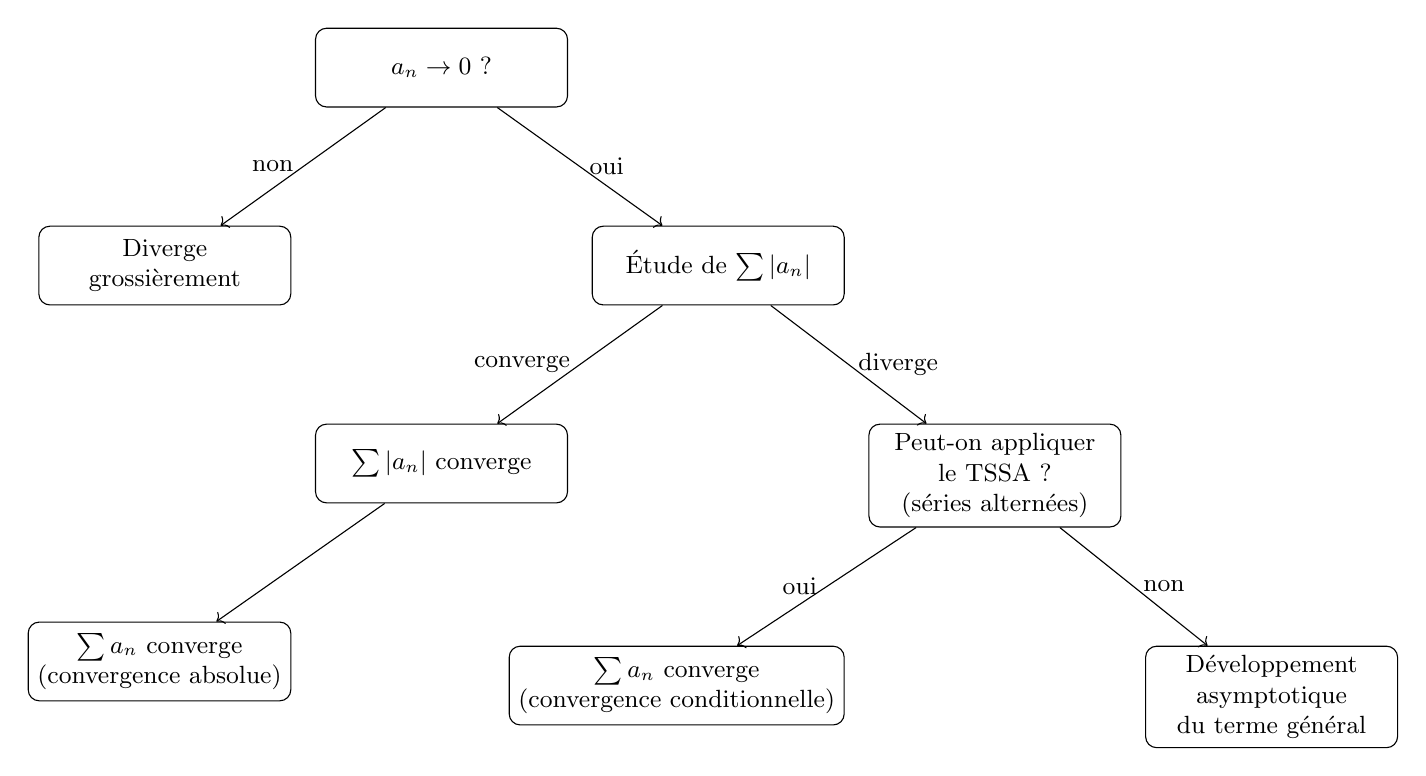
\begin{tikzpicture}[
    scale=0.85, % Réduction légère de l'échelle
    node distance=1.5cm and 0.3cm, % Espacement réduit
    every node/.style={align=center},
    box/.style={draw, rounded corners, minimum width=3.2cm, minimum height=1cm, font=\small} % Bulles un peu plus petites
]

% Structure en arbre vertical
% Niveau 1 : Point de départ
\node[box] (start) {$a_n \to 0$ ?};

% Niveau 2 : Première bifurcation
\node[box, below left=of start] (div) {Diverge\\grossièrement};
\node[box, below right=of start] (absstudy) {Étude de $\sum |a_n|$};

% Niveau 3 : Deuxième bifurcation depuis absstudy
\node[box, below left=of absstudy] (absconv) {$\sum |a_n|$ converge};
\node[box, below right=of absstudy] (applytssa) {Peut-on appliquer\\le TSSA ?\\(séries alternées)};

% Niveau 4 : Conclusions finales
\node[box, below left=of absconv] (seriecv1) {$\sum a_n$ converge\\(convergence absolue)};
\node[box, below left=of applytssa] (seriecv2) {$\sum a_n$ converge\\(convergence conditionnelle)};
\node[box, below right=of applytssa] (devtg) {Développement\\asymptotique\\du terme général};

% Flèches de l'arbre
\draw[->] (start) -- node[left, font=\small]{non} (div);
\draw[->] (start) -- node[right, font=\small]{oui} (absstudy);

\draw[->] (absstudy) -- node[left, font=\small]{converge} (absconv);
\draw[->] (absstudy) -- node[right, font=\small]{diverge} (applytssa);

\draw[->] (absconv) -- (seriecv1);
\draw[->] (applytssa) -- node[left, font=\small]{oui} (seriecv2);
\draw[->] (applytssa) -- node[right, font=\small]{non} (devtg);

\end{tikzpicture}
\end{center}

\vspace{1em}

\noindent
\textbf{Rappels de comparaison asymptotique :}

\begin{itemize}
  \item Si $a_n = b_n + O(w_n)$ où $\sum |w_n|$ converge, 
  alors $\displaystyle \sum_{n\ge0} a_n$ et $\displaystyle \sum_{n\ge0} b_n$ sont de même nature.

  \item Si $a_n = b_n + c_n + o(c_n)$ où $\sum b_n$ converge et $c_n > 0$, 
  alors $\displaystyle \sum_{n\ge0} a_n$ et $\displaystyle \sum_{n\ge0} c_n$ sont de même nature.
\end{itemize}



\begin{exemple}
    $\displaystyle a_n = \frac{(-1)^n}{n + (-1)^n\sqrt{n}}$ pour $n \geqslant 2$. 
    Etude de $\sum a_n$.

    $\abs{a_n} \sim \frac 1 n $ terme général série divergente donc pas de convergence absolue. 

    $\displaystyle \frac 1 {n + (-1)^n \sqrt n}$ n'est pas décroissante, on ne peut pas appliquer le TSSA. 

    \begin{align*}
        a_n & = \frac{(-1)^n} n \left[ \frac 1 {1 + \frac{(-1)^n} {\sqrt n}} \right] \\
            & = \frac{(-1)^n} n \left[ 1 - \frac{(-1)^n}{\sqrt n} + o\left( \frac 1 {\sqrt n} \right) \right] \\
            & = \underbrace{\frac{(-1)^n} n}_{\text{TGSCV par TSSA}} - \underbrace{\frac 1 {n^{3/2}} + o\left( \frac 1 {n^{3/2}} \right)}_{TGSCV}
    \end{align*}
    
    Donc $\sum a_n$ converge.

    \lvspace (exo 5) $u_n = \sin(n! \pi e)$ et $v_n = \sin(2 n! \pi e)$, $\displaystyle e = \sum_{k = 0 }^{ + \infty } \frac{1}{k!}$

    Donc :
    \begin{align*}
        n! e & = \sum_{k = 0 }^{+ \infty } \frac{n!}{k!} \\
              & = \underbrace{\sum_{k = 0}^{n - 2} \frac{n!}{k!}}_{\substack{P_n \text{ somme} \\ \text{d'entiers pairs}}} + n + 1 + \frac{1}{n + 1} + \frac{1}{(n + 1)(n + 2)} + \frac 1 {(n + 1)(n + 2)(n + 3)} + \sum_{k = n + 4 }^{\infty } \frac{n! }{k!} \\
    \end{align*}

    $\displaystyle \forall k \geqslant n + 4$, $\displaystyle \frac{n!}{k!} = \frac{1}{(n + 1)(n + 2) \cdots (k)} \leqslant \frac{1}{(n + 1)(n + 2)\ldots(k - 1)k}$

    \begin{align*}
        \sum_{k = n + 4 }^{+ \infty } \frac{n! }{k!} & \leqslant \sum_{k = n + 4 }^{\infty    }\frac 1 {(n + 1)(n + 2) (k-1)k} \\
                                                    & \leqslant \frac 1 {(n + 1)(n + 2)} \underbrace{\sum_{k = 2 }^{+ \infty } \frac 1 {(k - 1)k}}_C \\
    \end{align*}

    Donc $n ! e = qn + \frac 1 {n + 1} + O(\frac 1 {n^2})$ $a_n$ entier jsp quoi 

    \begin{align*}
        \sin(2 \pi n! e) & = \sin \left( 2 \pi \left( q_n + \frac 1 {n + 1} + O\left( \frac 1 {n^2} \right) \right) \right) \\
                                    & = \sin \left( 2 \pi \left( \frac 1 {n + 1} + O\left( \frac 1 {n^2} \right) \right) \right) \\
                                    & = \frac {2 \pi}{n + 1} + O\left( \frac 1 {n^2} \right) \\
    \end{align*}

    Donc $\sum v_n$ diverge. (La fin de la preuve est de copilot, pas eu la temps de noter, si qqun peut 
    vérifier que c'est bien ou m'envoyer le vrai truc, merci !) 
    
    \begin{align*}
        \sin(n! \pi e) & = \sin \left( \pi \left( q_n + \frac 1 {n + 1} + O\left( \frac 1 {n^2} \right) \right) \right) \\
                                    & = \sin \left( \pi \left( \frac 1 {n + 1} + O\left( \frac 1 {n^2} \right) \right) \right) \\
                                    & = (-1)^{q_n} \left( \frac{\pi}{n + 1} + O\left( \frac 1 {n^2} \right) \right) \\
    \end{align*}


\end{exemple}

\subsection{Sommation des relations de comparaison pour les séries divergentes}

Soient $\sum u_n$ et $\sum v_n$ deux séries réelles telles que $(v_n)$ est de signe constant à partir 
d'un certain rang. 

\begin{proposition}{Sommation des relations de comparaison}{}
\marginenote{Un peu d'histoire \!}{Les notations $o$ et $O$ viennent du mathématicien allemand Landau.}
    Si $\sum v_n$ diverge ($v_n$ de signe constant à partir d'un certain rang) et si $u_n = O(v_n)$ (resp $u_n = o(v_n)$, resp $u_n \sim v_n$),
    alors :
    
    $$\displaystyle \sum_{k = 1 }^{n }u_k = O\left( \sum_{k = 1}^{n} v_k \right)$$ 
    (resp $o$, resp $\sim$).
\end{proposition}

\begin{proof} $v_n > 0$ à partir d'un certain rang.
    
    \uline{Cas du O :}

    \svspace On suppose que $\exists M \in \R$, $\forall n \geqslant n_0, \, \abs{u_n} \leqslant M v_n$.
    Alors :
    \begin{align*}
        \abs{\sum_{k = 0 }^{n } u_k} & \leqslant \sum_{k=0 }^{n } \abs{u_k} \\
                                    & \leqslant \sum_{k = 0}^{n_0 - 1} \abs{u_k} + \sum_{k = n_0}^{n } M v_k \\
                                    & \leqslant \sum_{k = 0}^{n_0 - 1} \abs{u_k - M v_k} + M \sum_{k = 0}^{n } v_k \\
    \end{align*} 

    Or $\sum v_n$ diverge et $v_n > 0$ à partir d'un certain rang donc $\sum_{k = 0}^{n } v_k \longrightarrow + \infty$.

    \svspace Donc $\displaystyle \frac{\sum_{k = 0 }^{n_0 - 1} (\abs{u_k} - M v_k)}{ \sum_{k = 0}^n v_k} \longrightarrow 0 \leqslant 1$ pour $n > n_1$.

    \svspace Donc pour $\displaystyle n \leqslant \max(n_0, n_1)$, $\displaystyle \abs{\sum_{k = 0 }^{n } u_k} \leqslant \left( 1 + M \right) \sum_{k = 0}^{n } v_k$.

    Donc $\displaystyle \sum_{k = 0}^{n } u_k = O\left( \sum_{k = 0}^{n } v_k \right)$. \\

    \uline{Cas de $o$ :}

    \svspace On suppose que $\forall \varepsilon > 0, \exists n_0 \in \N, \, \forall n \geqslant n_0, \, \abs{u_n} \leqslant \varepsilon v_n$.
    Soit $\varepsilon > 0$. 

    Par le même calcul, $\exists n_0 \in \N, \, \exists n_1 \in \N$ tel que 

    $$\abs{\sum_{k = 0 }^{n } u_k} \leqslant \sum_{k = 0}^{n_0 - 1} (\abs{u_k} - \varepsilon v_k) + \varepsilon \sum_{k = 0}^{n } v_k$$

    et $\displaystyle \frac{\sum_{k = 0 }^{n_0 - 1} (\abs{u_k} - \varepsilon v_k)}{\sum_{k = 0}^{n } v_k} \leqslant \varepsilon$ 

    \svspace Donc pour $n \geqslant \max(n_0, n_1)$, $\displaystyle \abs{\sum_{k = 0 }^{n } u_k} \leqslant 2 \varepsilon \sum_{k = 0}^{n } v_k$.

    Donc $\displaystyle \sum_{k = 0}^{n } u_k = o\left( \sum_{k = 0}^{n } v_k \right)$. \\

    \uline{Cas de $\sim$ :}

    \svspace Supposons que $u_n \sim v_n$.

    Alors $\displaystyle u_n - v_n = o(v_n)$, donc $\displaystyle \sum_{k = 0}^{n } (u_k - v_k) = o\left( \sum_{k = 0}^{n } v_k \right)$.

    Donc $\displaystyle \sum_{k = 0}^{n } u_k = \sum_{k = 0}^{n } v_k + o\left( \sum_{k = 0}^{n } v_k \right) \sim \sum_{k = 0}^{n } v_k$.
\end{proof} 

\begin{proposition}{de Cesàro}{}
    Soit $(a_n)$ telle que $a_n \longrightarrow \ell \in \overline \R$. Alors :
    $$\frac 1 n \sum_{k = 1}^{n } a_k \longrightarrow \ell$$
    
\end{proposition}

\idee{Sommation des relations de comparaison.}

\begin{proof}
    \uline{Si $\ell \in \R^*$}, posons $v_n = \ell$, alors $\sum v_n$ diverge et $(v_n)$ est de signe constant.

    Or $\displaystyle a_n \sim v_n$ donc $\displaystyle \sum_{k = 1}^{n } a_k \sim \sum_{k = 1}^{n } v_k = n \ell$ (sommation des relations de comparaison). 

    Donc $\displaystyle \frac 1 n \sum_{k = 1}^{n } a_k \longrightarrow \ell$.

    \uline{Si $\ell = 0$}, alors $a_n = o(1)$, posons $v_n = 1$.
    De même, $\displaystyle \sum_{k = 1}^{n } a_k = o(n)$ donc $\displaystyle \frac 1 n \sum_{k = 1}^{n } a_k \longrightarrow 0$. \\

    \uline{Si $\ell = + \infty$ :} 

    \svspace Alors $a_n > 0 $ à partir d'un certain rang, et donc $1 = o(a_n)$.

    De même, $\displaystyle n = \sum_{k = 1}^{n } 1 = o\left( \sum_{k = 1}^{n } a_k \right)$ 

    Donc $\displaystyle 1 = o\left( \frac 1 n \sum_{k = 1}^{n } a_k \right)$ donc $\displaystyle \frac 1 n \sum_{k = 1}^{n } a_k \longrightarrow + \infty$.
\end{proof}



\begin{exemple}
    Pour obtenir un équivalent d'une somme partielle de série à termes positifs, 
    on peut espérer le trouver en utilisant la comparaison série intégrale.

    $\alpha > 0$, $\displaystyle S_n = \sum_{k = 0 }^{n } k^\alpha$. 

    Pour $\alpha = 1$, $\displaystyle S_n = \sum_{k = 0 }^{n } k = \frac{n(n + 1)}{2} \sim \frac{n^2}{2}$.

    Pour $\alpha = 2$, $\displaystyle S_n = \sum_{k = 0 }^{n } k^2 = \frac{n(n + 1)(2n + 1)}{6} \sim \frac{n^3}{3}$.

    Pour $\alpha = 3$, $\displaystyle S_n = \sum_{k = 0 }^{n } k^3 = \left( \frac{n(n + 1)}{2} \right)^2 \sim \frac{n^4}{4}$.

    Montrons qu'en général, $\displaystyle S_n \sim \frac{n^{\alpha + 1}}{\alpha + 1}$.

    Soit $k \geqslant 0$, $t \in [k, k + 1], \, k^\alpha \leqslant t^\alpha \leqslant (k + 1)^\alpha$.

    En intégrant sur $[k, k + 1]$, on trouve : $k^\alpha \leqslant \int_{k}^{k + 1} t^\alpha \text d t \leqslant (k + 1)^\alpha$

    Divisons par $k^\alpha$ : 
    $$ 1 \leqslant \frac 1 {k^\alpha} \int_{k}^{k + 1} t^\alpha \text d t \leqslant \left( \frac{k+1} k \right)^\alpha \longrightarrow 1$$

    Donc $k^\alpha \sim \int_{k }^{k + 1} t^\alpha \text d t$, or $\sum_{k \geqslant 0 } k^\alpha$ série à termes positifs divergente. 

    Donc par sommation des relation de comparaison, 

    $$S_n \sim \sum_{k = 0}^{n } \int_{k}^{k + 1} t^\alpha \text d t \sim \frac{n^{\alpha + 1}}{\alpha + 1}$$
\end{exemple}

\begin{remarque}
Pour généraliser cette idée il faut $f\in  \mathscr C^{pm}(\R^+, \R^+)$ monotone telle que $f(k+1) \sim f(k)$, on
montrerait de la même manière, dans le cas où $\int_0^n f(t) dt$ diverge, que $\sum_{k=1}^n f(k) \sim \int_0^n f(t) dt$.
\end{remarque}

\subsection{Sommation des relations de comparaison pour des séries convergentes}

\begin{theoreme}{Sommation des relations de comparaison}{}\\
    Soient $\sum u_n$ et $\sum v_n$ deux séries numériques telles que 
    $(v_n)$ est de signe constant à partir d'un certain rang et $\sum v_n$ converge.
    Supposons que $u_n = O(v_n)$ (resp $u_n = o(v_n)$, resp $u_n \sim v_n$).

    Alors $\sum u_n$ converge et on peut donc définir les restes des deux séries, et 
    $\displaystyle R_n(u) = O(R_n(v))$ (resp $o$, resp $\sim$).
\end{theoreme}

\begin{proof}
    La convergence de $\sum u_n$ est immédiate par comparaison. 

    \uline{Si $u_n =  O(v_n)$}, alors $\exists M > 0, \exists n_0 \in \N, \, \forall k \geqslant n_0, \, \abs{u_k} \leqslant M \abs{v_k}$.

    Donc $\displaystyle \forall n \geqslant n_0, \, \forall N > n, \, \abs{\sum_{k = n + 1 }^{N } u_k} \leqslant \sum_{k = n + 1 }^{N } \abs{u_k} \leqslant M \sum_{k = n + 1}^{N } \abs{v_k}$.

    Par passage à la limite, $\abs{R_n(u)} \leqslant M \abs{R_n(v)}$ car $v_k$ de signe constant. 
    Donc $R_n(u) = O(R_n(v))$. \\

    \uline{Si $u_n = o(v_n)$,} 
    on fait le même raisonnement avec $\forall \varepsilon$ à la place de $\exists M$. \\

    \uline{Si $u_n \sim v_n$}, alors $u_n - v_n = o(v_n)$. 

    Donc $R_n(u - v) = o(R_n(v))$ donc $R_n(u) = R_n(v) + o(R_n(v)) \sim R_n(v)$.
\end{proof}

\begin{exemple}
    Cherchons l'équivalent du reste d'une série de Riemann convergente. 

    Soit $\alpha > 1$, $\displaystyle \sum_{k = n + 1}^{+ \infty } \frac 1 {k^\alpha}$.

    Posons $\displaystyle v_k = \int_k^{k + 1} \frac 1 {t^\alpha} \text d t$. 

    $\displaystyle \forall t \in [k, k + 1], \, \frac 1 {(k + 1)^\alpha} \leqslant \frac 1 {t^\alpha} \leqslant \frac 1 {k^\alpha}$

    Donc $\displaystyle \left( \frac k {k +  1} \right)^\alpha \leqslant \frac {v_k}{u_k} \leqslant 1$.

    Donc $v_k \sim u_k$.
    Donc $R_n(u) \sim R_n(v)$, or 

    \begin{align*}
        \sum_{k = n + 1 }^{N } v_k & = \sum_{k = n + 1}^{N } \int_k^{k + 1} \frac 1 {t^\alpha} \text d t \\
                                            & = \int_{n + 1}^{N + 1} \frac 1 {t^\alpha} \text d t \\
                                            & = \left[ \frac{t^{1 - \alpha}}{1 - \alpha} \right]_{n + 1}^{N + 1} \\
                                            & = \frac 1 {\alpha - 1} \left( \frac 1 {(n + 1)^{\alpha - 1}} - \frac 1 {N + 1}^{\alpha - 1} \right) \\
                                            & \sim \frac 1 {\alpha - 1} \frac 1 {(n + 1)^{\alpha - 1}} 
    \end{align*}

    Donc $\displaystyle \sum_{k = n + 1}^{\infty} \frac 1 {k^\alpha} \sim \frac 1 {\alpha - 1} \frac 1 {(n + 1)^{\alpha - 1}}$. \\
\end{exemple}     

\begin{exemple}
    Trouvons maintenant l'équivalent de $\displaystyle \sum_{k = n + 1}^{\infty } \frac 1 {k^2} = R_n$.
    On a $\displaystyle \frac 1 {k^2} \sim \frac 1 {k(k + 1)}$.

    Or $\displaystyle \sum_{k = n + 1}^{N} \frac 1 {k(k + 1)} = \sum_{k = n + 1}^{N } \left( \frac 1 k - \frac 1 {k + 1} \right) = \frac 1 {n + 1} - \frac 1 {N + 1}$

    Donc $\displaystyle R_n \sim \frac 1 n$.
    Or par sommation des relations de comparaison, 
    
    \center{$\displaystyle \sum_{k = n + 1}^{\infty } \frac 1 {k^2} \sim \sum_{k = n + 1}^{\infty } \frac 1 {k(k + 1)} \sim \frac 1 {n + 1} \sim \frac 1 n$.}
\end{exemple}



\pagevide
\chapitreintegral{5}{Familles sommables}
\displaychapitrebanner
\section{Dénombrabilité}
\subsection{Définitions}

\begin{definition}{Dénombrable}{}
    Soit $I$ un ensemble. On dit que $I$ est \emph{dénombrable} 
    s'il existe une bijection entre $\N$ et $I$.
    On dira que $I$ est \emph{équipotent} à $\N$ (LHP).
\end{definition}

\begin{exemple}
    \begin{itemize}
        \item L'ensemble $\N$ est dénombrable (la bijection est l'identité).
        \item L'ensemble $\N^*$ est dénombrable (la bijection est $f : n \mapsto n+1$).
        \item $2 \N$ est dénombrable (la bijection est $f : n \mapsto 2n$).
        \item $\Z$ est dénombrable (la bijection est $f : n \mapsto p \text{ ou } -p-1$ selon la parité de $n$).
    \end{itemize}
\end{exemple}


\begin{definition}{Au plus dénombrable}{}
    Soit $I$ un ensemble. On dit que $I$ est \emph{au plus dénombrable} si $I$ est 
    fini ou dénombrable.
\end{definition}

\subsection{Cas des parties de \texorpdfstring{$\N$}{N}}

\begin{theoreme}{Nature des parties infinies de $\N$}{}
    Toute partie infinie de $\N$ est dénombrable.
\end{theoreme}

\idee{
    On numérote les éléments de $A$ par ordre croissant en construisant une 
    bijection et des récurrences.
}

\begin{proof}
    Soit $A \subset \N$ infinie. 

    Construisons par récurrence $\varphi : \N \to A$ en posant : $\varphi(0) = \min(A)$ car $A \neq \emptyset$.

    Et par récurrence, $\forall n \in \N, \, \varphi(n+1) = \min(\underbrace{A \setminus \underbrace{\{\varphi(0), \ldots, \varphi(n)\}}_{\text{est fini}}}_{\text{infini donc non vide}})$. \\

    \uline{Montrons que $\varphi$ est bijective :}

    \svspace On a $\varphi(n) = \min(\underbrace{A \setminus \{\varphi(0), \ldots, \varphi(n-1)\}}_{= B })$ 
    et $\varphi(n + 1) = \min(B \setminus \{ \varphi(n) \})$ 

    Donc $\forall k \in B, \, \varphi(n) \leqslant k$ et $\exists k_1 \in B \setminus \{\varphi(n)\}, \, \varphi(n + 1) = k_1$

    Donc $\varphi(n) \leqslant \varphi(n + 1)$ et $\varphi (n) \neq \varphi(n + 1)$ par construction.

    Donc $\varphi(n) < \varphi(n + 1)$, donc $\varphi$ est injective. \\

    Soit $a \in A$, alors $\{k \in A | k < a\}$ est fini et $(\varphi(n))_{n \in \N}$ est strictement croissante, donc
    $\exists n_0 \in \N, \, \varphi(n_0) \geqslant a$.

    Soit $n_0$ le plus petit entier tel que $\varphi(n_0) \geqslant a$.

    On a donc $\varphi(n_0 - 1) < a \leqslant \varphi(n_0)$.
  
    Donc $a = \varphi(n_0)$ par construction, donc $\varphi$ est surjective.
\end{proof}

\begin{proposition}{Nature des parties de $\N$}{}
    Dans $\N$, il y a deux types de parties : 
    \begin{itemize}
        \item Les parties majorées qui sont finies.
        \item Les parties non majorées qui sont infinies et dénombrables.
    \end{itemize}

    Toute partie de $\N$ est donc au plus dénombrable. 
\end{proposition}


\begin{proposition}{Caractérisation des ensembles au plus dénombrables}{}
    Soit $E$ un ensemble non vide. Alors $E$ est au plus dénombrable ssi il est en 
    bijection avec une partie de $\N$.
\end{proposition}


\begin{proof}
    $\Leftarrow$ Si $E$ est en bijection avec $I \subset \N$, alors si $I$ est finie, 
    $E$ l'est également, et si $I$ est infinie, alors $I$ est dénombrable donc $E$ aussi.

    $\Rightarrow$ Si $E$ est au plus dénombrable, alors si $E$ est fini, il est en bijection 
    avec $\ninter 1 {\text{Card}(E)} \subset \N$.
    S'il est dénombrable, par définition il est en bijection avec $\N$.
\end{proof}


\subsection{Opérations}

\begin{theoreme}{}{}
    $\N^2$ est dénombrable.
\end{theoreme}

\begin{proof} (non exigible)
    Considérons $\fonction \varphi {\N^2} \N {(p, q)}{2^p (2q + 1) - 1}$.

    $\varphi$ est bien définie, et si $a \in \N$, alors $a + 1 \in \N^*$, donc possède 
    une unique décomposition en facteurs premiers qui fournit $p$ et $q$ en isolant 
    la contribution de $2$ et le produit impair des autres premiers. 
\end{proof}

\begin{proposition}{Opérations conservant le caractère dénombrable}{}
    \begin{itemize}
        \item $\forall p \in \N, \, \N^p$ est dénombrable.
        \item Tout produit cartésien fini d'ensembles dénombrables est dénombrable.
    \end{itemize}

\end{proposition}

\idee{Par récurrence.}

\begin{proof}
    Par récurrence : 
    \begin{itemize}
        \item $\N^1$ est dénombrable 
        \item Supposons que $\N^p$ est dénombrable pour un certain $p$. Cela fournit $\varphi : \N \to \N^p$ bijective. 
    \end{itemize}

    Considérons $\psi : \N^2 \to \N$ bijective. Posons alors $\fonction f {\N^{p + 1}} \N {(n_1, \cdot, n_{p + 1})} {\psi(\varphi^{-1}(n_1, \ldots, n_p), n_{p + 1})}$.

    Alors $f$ est bijective. 

    \lvspace Soient $E_1, \ldots, E_n$ des ensembles dénombrables.

    Posons pour tout $i, \varphi_i : E_i \to \N$ bijective et $f : \N^p \to \N$ bijective.

    Alors $\fonction{}{E_1 \times \cdot \times E_p} \N {(e_1, \ldots, e_p)} {f(\varphi_1(e_1), \ldots, \varphi_p(e_p))}$ est bijective.
\end{proof}

\begin{theoreme}{}{}
    $\Z$ est dénombrable.
\end{theoreme}

\begin{proof}
Posons $\varphi : x \mapsto \frac n 2$ si $n \in 2 \N$ et $-(\frac {n+1} 2)$ sinon.

Alors $\varphi$ est injective et surjective dans $\Z$ donc elle est bijective.
Donc $\Z$ est équipotent à $\N$ donc $\Z$ est dénombrable.
\end{proof}

\begin{theoreme}{}{}
    $\Q$ est dénombrable. 
\end{theoreme}

\idee{
    Bijection qui associe à chaque rationnel le couple (numérateur, dénominateur)
    irréductible.
}

\begin{proof}
    Considérons $\fonction \varphi \Q {\Z \times \N^*}{\underbrace{ x = \frac p q}_{\text{irréductible}} } {(p, q)}$.

    $\varphi$ est bien définie et injective, car si $\varphi(x) = (p, q)$, alors $x = \frac p q$

    Mais $\Z \times \N^*$ est dénombrable, donc $\varphi(\Q) \subset \Z \times \N^*$ est 
    au plus dénombrable. 

    Or $\varphi(\Q)$ est en bijection avec $\Q$, donc $\Q$ est au plus dénombrable, or $\Q$ est 
    infini, donc $\Q$ est dénombrable.
\end{proof}

\begin{theorement}{Nature d'une union au plus dénombrable d'ensemble au plus dénombrables}{}
    Toute union \textbf{finie ou dénombrable} d'ensembles au plus dénombrables est au plus dénombrable. 
\end{theorement}

\begin{proof} (non exigible)\\
    Soit $I$ non vide au plus dénombrable.
    
    Pour $i \in I, \, I \subset \N$, il existe $P_i \subset \N$ non vide et $\fonction {\varphi_i} {P_i} {E_i} n {\varphi_i(n) }$ bijective. 

    Considérons $\fonction {\psi_i} {E_i} \N x {\varphi_i^{-1}(x)}$ alors $\psi_i$ n'est pas forcément 
    surjective mais elle est injective. 

    Considérons maitenant $\fonction {\psi} {\bigcup_{i \in I} E_i} {\N^2} x {(i, \psi_i(x))}$ où $i = \min \{ \alpha \in \N, \, x \in E_\alpha \}$.

    $\psi$ est bien définie, et $\psi$ est injective, car si $x = y = (i, j)$, 
    on a $x, y \in E_i$ et $j = \psi_i(x) = \psi_i(y)$, donc $x = y = \varphi_i(j)$.

    Donc $\displaystyle \bigcup_{i \in I} E_i$ est en bijection avec son image par $\psi$
    qui est une partie de $\N^2$, qui est donc au plus dénombrable.

\end{proof}

\subsection{Ensembles non dénombrables}

\begin{theoreme}{Nature de $\R$}{}
    $\R$ est non dénombrable.
\end{theoreme}

\begin{proof} (non exigible)
    Par l'absurde, supposons que $\varphi : \N \to \R$ est bijective. 

    Comme $\fonction{} \R {]0, 1[} x {\frac 1 {1 + e^{- x}}}$ est bijective, donc 
    il existe une bijection de $\N$ dans $]0, 1[$.

    Considérons pour $i \in \N^*$ la $i + 1^{\text{eme}}$ décimale du développement décimal 
    propre de $\varphi(i)$. Notons la $a_i$. 

    Posons $b_i = 4$ si $a_i \neq 4$ et $b_i = 5$ sinon, et posons $\displaystyle y = \sum_{i = 1}^{+ \infty} \frac{b_{i + 1}}{10^i} \in ]0, 1[$ 

    Posons $j = \psi^{-1}(y)$,
    la jème décimale de $y$ est $b_j$ par définition de $y$ sa $j$e décimale est 
    $a_j$, absurde. Donc $\psi \circ \varphi$ non bijective.
\end{proof}

\begin{theoreme}{Non équipotence de $E$ et $\mathscr P(E)$ - LHP}{}
    Soit $E$ un ensemble non vide. Alors il n'existe pas de bijection entre $E$ et $\mathscr P(E)$.
\end{theoreme}

\begin{proof}
    Par l'absurde, si $\fonction \psi E {\mathscr P(E)} x {\psi(x)}$ est bijective,

    Considérons $B = \{ x \in E | x \notin \psi(x) \} $ et $x_0 = \psi^{-1}(B)$.

    Si $x_0 \in B, \, x_0 \notin \psi(x_0) = B$ absurde.

    Si $x_0 \notin B, \, x_0 \in \psi(x_0)$ donc $x_0 \in B$ absurde. 
\end{proof}

\begin{remarque}
    On montrerait que $\mathscr P(\N)$ est en bijection avec $\R$.
\end{remarque}

\section{Familles sommables}
\subsection{Définition et premières propriétés}

\begin{definition}{Famille sommable}{}
    Soit $I$ un ensemble non vide et $(u_j)_{j \in I}$ une famille de complexes indexée par $I$. 
    On dit que cette famille est sommable ssi l'ensemble 
    $$\left\{\sum_{j \in J} |u_j|, \, J \subset I \text{ fini} \right\}$$
    est majoré. 
\end{definition}

\begin{proposition}{Stabilité par combinaison linéaire}{}
    Soit $(u_j)_{j \in I}$ une famille sommable de complexes et $I' \subset I$ non vide.
    \begin{itemize}
        \item Alors $(u_j)_{j \in I'}$ est sommable. 
        \item Si $(v_j)$ est une autre famille sommable, et $\alpha, \beta \in \C$, alors 
        $(\alpha u_j + \beta v_j)_{j \in I}$ est sommable.
    \end{itemize}
\end{proposition}

\idee{Majorer les sommes partielles.}

\begin{proof}
    Par hypothèse, $\exists M_1, M_2 > 0, \, \forall J \subset I$ fini, 

    $\displaystyle \sum_{j \in J} |u_j| \leqslant M_1$ et $\displaystyle \sum_{j \in J} |v_j| \leqslant M_2$.

    Soit $J \subset I'$ fini, alors $J \subset I$ donc $\sum_{j \in J } |u_j| \leqslant M_1$.

    Donc $(u_j)_{j \in I'}$ est sommable.

    Soit $J \subset I$ fini, alors
    $$\sum_{j \in J} |\alpha u_j + \beta v_j | \leqslant \sum_{j \in J} (|\alpha| |u_j| + |\beta| |v_j|) \leqslant |\alpha| M_1 + |\beta| M_2$$
\end{proof}

\subsection{Somme d'une famille sommable}

\begin{proposition}{Inégalité de comparaison}{}
    Soit $(u_j)_{j \in I}$ une famille sommable de complexes et $(v_j)_{j \in I}$
    une autre famille telle que $\forall j \in I, \, |v_j| \leqslant |u_j|$.

    Alors $(v_j)_{j \in I}$ est sommable.
\end{proposition}

\begin{proof}
    Soit $J \subset I$ fini, alors :
    $$\sum_{j \in J} |v_j| \leqslant \sum_{j \in J} |u_j| \leqslant M$$
\end{proof}


\begin{definition}{Somme d'une famille sommable}{}\\
    Soit $(u_i)_{i \in I}$ une famille sommable de réels positifs. 

    Alors $\displaystyle \left\{ \sum_{i \in J} u_i, \, J \subset I \text{ fini}  \right\}$ est une partie 
    de $\R$. 

    Sa borne supérieure est appellée \emph{somme} de la famille et notée $\displaystyle \sum_{i \in I} u_i$.
    Ainsi : $$\sum_{i \in I} u_i = \sup \left\{ \sum_{i \in J} u_i, \, J \subset I \text{ fini}  \right\}$$
\end{definition}

\begin{theoreme}{Somme d'une famille sommable de réels quelconques}{}
    Soit $(u_j)_{i \in I}$ une famille de réels. 
    Posons $\forall i \in I : $ 
    \begin{align*}
        u_i^+ = \frac 1 2 (|u_i| + u_i)\\
        u_i^- = \frac 1 2 (|u_i| - u_i)
    \end{align*}

    Alors $(u_j)_{j\in I}$ est sommable ssi $(u_j^+)_{j\in I}$ et $(u_j^-)_{j\in I}$ sont sommables.

    On définit la somme de la famille $(u_j)_{i \in I}$ par :
    $$\sum_{i \in I} u_i = \sum_{i \in I} u_i^+ - \sum_{i \in I} u_i^-$$
\end{theoreme}
\marginenote{Remarque}{Cette définition est bien compatible avec la def 5.17 dans le
cas où $\forall j\in\mathbb{B}, U_j\geqslant 0$.}
\begin{proof}{}{}

    $\Rightarrow$ On a $\left\{\begin{array}{cc}
        |u_j^+| \leqslant |u_j|\\
        |u_j^-| \leqslant |u_j|
    \end{array}\right.$, d'où l'implication par la proposition 5.16.\\

    $\Leftarrow$ Supposons que $(u_j^+)_{j\in I}$ et $(u_j^-)_{j\in I}$ sont sommables. Soit $J\subset I$ fini non vide

    $$\sum_{j\in J} |u_j|\leqslant\sum_{j\in J} U_j^+ + \sum_{j\in J} U_j^-\leqslant \sum_{j\in I} U_j^+ + \sum_{j\in I} U_j^- \leftarrow\text{constante indépendante de J}$$

    \end{proof}



\begin{theoreme}{Somme d'une famille sommable de complexes}{}

    Soit $(u_j)_{j \in I}$ une famille de complexes. Alors :
    
    $(u_j)_{j\in I}$ est sommable ssi $(\re(u_j))_{j\in I}$ et $(\im(u_j)_{j\in I}$ le sont.

    On définit la somme de la famille $(u_j)_{j \in I}$ par :
    $$\sum_{j \in I} u_j = \sum_{j \in I} \re(u_j) + i \sum_{j \in I} \im(u_j)$$

\end{theoreme}

\idee{Utiliser la proposition 5.16.}
\begin{proof}{}{}
    $\Rightarrow$
    $\begin{array}{cc}
    |\re(u_j)| \leqslant |u_j| \\
    |\im(u_j)| \leqslant |u_j|
    \end{array}$

    $\Leftarrow
    |u_j|\leqslant |\re(u_j)| + |\im(u_j)|$

\end{proof}

\begin{proposition}{Linéarité de la somme}{}
    Soit $(u_j)_{j \in I}, (v_j)_{j \in I}$ deux familles sommables de complexes et $\alpha, \beta \in \C$.

    Alors $(\alpha u_j + \beta v_j)_{j \in I}$ est sommable et :
    $$\sum_{j \in I} (\alpha u_j + \beta v_j) = \alpha \sum_{j \in I} u_j + \beta \sum_{j \in I} v_j$$
\end{proposition}

\begin{proof}
    Le faire d'abord pour des réels positifs, puis des réels quelconques, puis des complexes.
\end{proof}

\begin{theoreme}{Sommation par paquets}{}
    Soient $I$ et $K$ des ensembles non vides et $\displaystyle I = \bigsqcup_{k \in K} I_k$ union
    disjointe d'ensembles non vides.

    Soit $(u_j)_{j \in I}$ une famille de complexes. Alors $(u_j)_{j \in I}$ est sommable ssi
    
    $\forall k \in K, \, (u_j)_{j \in I_k}$ est sommable et $\displaystyle \left( \sum_{j \in I_k} |u_j| \right)_{k \in K}$ est sommable
    et en ce cas, 
    $$ \sum_{j \in I} u_j = \sum_{k \in K} \left( \sum_{j \in I_k} u_j \right)$$
\end{theoreme}

\subsection{Conséquence : permutation des termes}

\begin{theoreme}{Invariance par bijection}{}
    Soit $(u_j)_{j \in I}$ une famille sommable de complexes et $\sigma: I \to I$ une bijection 
    alors $(u_{\sigma(j)})_{j \in I}$ est sommable et $\displaystyle \sum_{j \in I} u_j = \sum_{j \in I} u_{\sigma(j)}$.
\end{theoreme}

\begin{proof}
    Posons $K = I$ et $\forall k \in K, \, I_k = \{\sigma(k)\}$.

    $\sigma$ étant une bijection, $\displaystyle I = \bigsqcup_{k \in K} I_k$.

    $(u_j)_{j \in I_k}$ étant sommable, par le théorème de sommation par paquets, 
    $\forall k \in K, \, (u_j)_{j \in I_k}$ est sommable 
    et comme $\displaystyle \sum_{j \in I_k} |u_j| = |u_{\sigma(k)}|$,
    on a que $(u_{\sigma(k)})_{k \in K}$ est sommable, et :
    $$\sum_{j \in I} u_j = \sum_{k \in K} \left( \sum_{j \in I_k} u_j \right) = \sum_{k \in K} u_{\sigma(k)} = \sum_{j \in I} u_{\sigma(j)}$$
\end{proof}

\subsection{Lien avec la dénombrabilité}

\begin{definition}{Support d'une famille}{}
    Soit $(u_j)_{j \in I}$ une famille de complexes. On appelle support de cette 
    famille l'ensemble $\{j \in I ~|~ u_j \neq 0 \}$.
\end{definition}

\begin{proposition}{Somme sur le support}{}
    Soit $(u_j)_{j \in I}$ une famille sommable de complexes de support $S$. Alors :
    $$\sum_{j \in I} u_j = \sum_{j \in S} u_j$$
\end{proposition}


\begin{proof}
    Posons $K = \{1, 2\}$, et $I_1 = S, \, I_2 = I \setminus S$.

    Par le théorème de sommation par paquets, $\displaystyle \sum_{j \in I} u_j = \sum_{j \in S} u_j + \sum_{j \in I \setminus S} u_j$.
\end{proof}

\begin{theoreme}{Nature du support d'une famille sommable}{}
    Le support d'une famille sommable est au plus dénombrable. 
\end{theoreme}

\begin{proof}
    Soit $(u_j)_{j \in I}$ une famille sommable de complexes. 

    Posons $I_0 = \{j \in I, \, 1 < |u_j| \}$, et pour $n \in \N^*$,
    $I_n = \{j \in I, \, \frac 1 {n + 1} < |u_j| \leqslant \frac 1 n \}$.

    Montrons que $\displaystyle S = \bigsqcup_{n \in \N} I_n$. 

    $\subset$ $\forall n \in \N, \, I_n \subset S$ car $\forall j \in I_n, \, u_j \neq 0$
    Si $n \neq n', \, I_n \cap I_{n'} = \emptyset$ donc $\displaystyle \bigsqcup_{n \in \N} I_n \subset S$.

    $\supset$ $j \in S$, alors $\mid u_j \mid > 0$, on a donc $\displaystyle j \in I_{\left\lfloor \frac 1 {|u_j|} \right\rfloor}$, 
    donc $S \subset \displaystyle \bigsqcup_{n \in \N} I_n$.

    Soit $k \in \N$, alors $\forall j \in I_k, \, \frac 1 {k + 1} < \underbrace{|u_j|}_{\text{sommable}}$

    Donc $\left( \frac 1 {k + 1} \right)_{j \in I_k}$ est sommable, or $\frac 1 {k + 1}$ est constant et positif, 

    donc $I_k$ est fini, donc $S$ est au plus dénombrable.
\end{proof}

\section{Familles indexées par \texorpdfstring{$\N$}{N}}
\subsection{Théorème}

\begin{theoreme}{Familles sommables indexées par $\N$}{}
    Soit $(u_n)_{n \in N}$ une famille de complexes. Alors
    cette famille est sommable ssi $\displaystyle \sum_{n \geqslant 0} u_n$ est 
    absolument convergente et alors :
    $$\sum_{n \in \N} u_n = \sum_{n = 0}^{+\infty} u_n$$    
\end{theoreme}

\begin{proof}
    $\Rightarrow$ Supposons que $(u_n)_{n \in \N}$ est sommable. 

    Ainsi $\forall J \subset \N$ fini, $\displaystyle \sum_{n \in J} |u_n| \leqslant M$.

    Soit $N \in \N$, alors $\displaystyle \sum_{j = 0 }^N |u_j|  = \sum_{n \in \{0, \ldots, N\}} |u_n| \leqslant M$.

    Donc $\sum_{j \geqslant 0} |u_j|$ converge et la série est absolument convergente. 

    \lvspace $\Leftarrow$ Supposons que $\sum_{n \geqslant 0} |u_n|$ converge. 

    Soit $J \subset \N$ fini, et soit $N \in \N$ un majorant de $J$. 

    $$\sum_{j \in J} |u_j| \leqslant \sum_{j = 0}^N |u_j| \leqslant \sum_{j = 0}^{+\infty} |u_j|$$

    Donc la famille est sommable. \\

    \uline{Si $\forall n, \, u_n \in \R^+$ :}
    Pour $J \subset \N$ fini, soit $N$ un majorant de $J$. 
    $$\sum_{j \in J} u_j \leqslant \sum_{j = 0}^N u_j \leqslant \sum_{j = 0}^{+\infty} u_j$$

    Par définition de la borne sup, 
    $$\sum_{n \in \N} u_n \leqslant \sum_{j = 0 }^{+\infty} u_j$$

    Par ailleurs $\forall k \in \N, \, \displaystyle \sum_{i = 0}^k u_i  = \sum_{i \in \ninter 0 n} u_i \leqslant \sum_{i \in \N} u_i$.

    Donc par passage à la limite, $\displaystyle \sum_{i = 0}^{+\infty} u_i \leqslant \sum_{i \in \N} u_i$ et on a donc l'égalité. \\

    \uline{Si $\forall n \in \N, \, u_n \in \R$ :}
    $a \leqslant u_n^+ \leqslant |u_n|$ et $0 \leqslant u_n^- \leqslant |u_n|$.

    Donc par ce qui précède, 
    $$\sum_{n = 0}^{+ \infty} u_n^+ = \sum_{n \in \N} u_n^+ \text{ et } \sum_{n = 0}^{+\infty} u_n^- = \sum_{n \in \N} u_n^-$$

    Et donc par défférence, $\displaystyle \sum_{n = 0}^{+\infty} u_n = \sum_{n \in \N} u_n$.

    Dans le cas complexe, on a l'égalité pour les parties réelles et imaginaires, d'où la conclusion 
    par combinaison linéaire. 
\end{proof}

\subsection{Conséquence}

\begin{proposition}{Sommation par paquets pairs et impairs - LHP}{}
    Soit $\sum_{n \geqslant 0} u_n$ une série absolument convergente, alors :
    $$\sum_{n  = 0 }^{+\infty} u_n = \sum_{p = 0 }^{+\infty} u_{2p} + \sum_{p = 0}^{+\infty} u_{2p + 1}$$
\end{proposition}

\begin{proof}
    La famille est sommable, et on applique le théorème de sommation par paquets. 
\end{proof}

\begin{exemple}
    Calcul de $\displaystyle S = \sum_{n = 0 }^{+\infty} \frac 1 {(2n + 1)^2}$, qui existe car le terme général est équivalent à $\frac 1 {n^2}$. 

    $\displaystyle \zeta(2) = \frac{\pi^2} 6 = \sum_{n = 1}^{+\infty} \frac 1 {n^2}$ famille sommable. 

    $\displaystyle \zeta(2) = \sum_{n = 0 }^{+\infty} \frac 1 {(2n)^2} + \sum_{n = 0 }^{+\infty} \frac 1 {(2n + 1)^2}$ par le th de sommation par paquets. 

    $\displaystyle \frac{\pi^2} 6 = S + \frac{\pi^2}{24}$

    Donc $S = \frac {\pi^2} 8$.
\end{exemple}

\subsection{Commutative convergence}

\begin{theoreme}{Invariance par bijection de $\N$}{}
    Soit $\displaystyle \sum_{n \geqslant 0} u_n$ une série absolument convergente et $\sigma : \N \to \N$ une bijection.
    Alors $\displaystyle \sum_{n =\geqslant 0} u_{\sigma(n)}$ est absolument convergente et :
    $$\sum_{n = 0}^{+\infty} u_n = \sum_{n = 0}^{+\infty} u_{\sigma(n)}$$
\end{theoreme}

\begin{proof}
    $(u_n)_{n \in \N}$ est sommable car la série converge absolument,
    on réutilise donc le résultat prouvé avant.
\end{proof}

\begin{remarque}
    Si la série est semi-convergente, c'est faux.
\end{remarque}


\section{Famillles indexées par \texorpdfstring{$\N^2$}{N²}}
\subsection{Cas des familles réelles positives}

\begin{theoreme}{}{}
    Soit $(u_{n, p})_{(n, p) \in \N^2}$ une famille de \textbf{réels positifs}.
    Alors les assertions suivantes sont équivalentes :
    \begin{enumerate}
        \item la famille $(u_{n, p})_{(n, p) \in \N^2}$ est sommable
        \item $\ds \forall n \in \N, \, \sum_{p \geqslant 0 } u_{n, p}$ converge et $\ds \sum_{n \geqslant 0} \left(\sum_{p = 0}^{+\infty} u_{n, p} \right)$ converge.
        \item $\ds \forall p \in \N, \, \sum_{n \geqslant 0 } u_{n, p}$ converge et $\ds \sum_{p \geqslant 0} \left(\sum_{n = 0}^{+\infty} u_{n, p} \right)$ converge.
        \item En posant $\ds \forall k \in \N, \, w_k = \sum_{n = 0 }^{k }u_{n, k - n} = \sum_{p = 0 }^{k } u_{k - p, p} = \sum_{\substack{(n, p) \in \N^2 \\ n + p = k}} u_{n, p}$, la série $\ds \sum_{k = 0}^{+\infty} w_k$ converge
            et en ce cas $\ds \sum_{(n, p) \in \N^2} u_{n,p} = \sum_{n = 0}^{+\infty} \sum_{p = 0}^{+\infty}u_{n, p} = \sum_{p = 0}^{+\infty} \sum_{n = 0}^{+\infty}u_{n, p} = \sum_{k = 0 }^{+\infty} w_k$ 
    \end{enumerate}
\end{theoreme}

\begin{proof}
    C'est le théorème de sommation par paquets appliqué aux partitions de
    $\N^2 = \bigsqcup_{n \in \N} I_n = \bigsqcup_{p \in \N} J_p = \bigsqcup_{k \in \N} E_k$
    où $I_n = \{ (n, p), \, p \in \N \}, \, J_p = \{ (n, p), \, n \in \N \}$ et
    $E_k = \{ (n, p), \, n + p = k \}$.
\end{proof}

\subsection{Théorème de Fubini positif}

\begin{theoreme}{Théorème de Fubini positif}{}
    Avec la convention qu'une somme infinie non convergente de réels positifs vaut 
    $+ \infty$ on a pour toute famille de \textbf{réels positifs} $(u_{n, p})_{(n, p) \in \N^2}$ :
    $$\sum_{n = 0}^{+\infty} \left(\sum_{p = 0}^{+\infty} u_{n, p} \right) = \sum_{p = 0}^{+\infty} \left( \sum_{n = 0}^{+\infty} u_{n, p} \right) $$
\end{theoreme}

\begin{proof}
    Conséquence du 1. de la proposition précédente.
\end{proof}

\subsection{Cas général}

\begin{theoreme}{}{}
    Soit $(u_{n, p})_{(n, p) \in \N^2}$ une famille sommable de complexes. Alors :

    \begin{enumerate}
        \item $\ds \forall n \in \N, \, \sum_{p \geqslant 0 } u_{n, p}$ converge et $\ds \sum_{n \geqslant 0} \left( \sum_{p = 0}^{+\infty} u_{n, p} \right)$ converge.
        \item $\ds \forall p \in \N, \, \sum_{n \geqslant 0 } u_{n, p}$ converge et $\ds \sum_{p \geqslant 0} \left( \sum_{n = 0}^{+\infty} u_{n, p} \right)$ converge.
        \item En posant $\ds \forall k \in \N, \, w_k = \sum_{n = 0 }^{k }u_{n, k - n} = \sum_{p = 0}^{k} u_{k - p, p} = \sum_{\substack{(n, p) \in \N^2 \\ n + p = k}} u_{n, p}$, la série $\ds \sum_{k = 0}^{+\infty} w_k$ converge
            et en ce cas $\ds \sum_{(n, p) \in \N^2} = \sum_{n = 0 }^{+\infty} \sum_{p = 0}^{+\infty}u_{n, p} = \sum_{p = 0}^{+\infty} \sum_{n = 0}^{+\infty}u_{n, p} = \sum_{k = 0}^{+\infty} w_k$ 
    \end{enumerate}
\end{theoreme}

\subsection{Produit de Cauchy}

\begin{theoreme}{Produit de Cauchy}{}
    Soient $ \sum_{n \geqslant 0} u_n$ et $ \sum_{n \geqslant 0} v_n$ deux séries 
    numériques \textbf{absolument convergentes}.
    
    On définit la suite $(w_n)_{n \in \N}$ appelée produit de convolution des suites 
    $(u_n)_{n \in \N}$ et $(v_n)_{n \in \N}$ par :
    $$\forall n \in \N, \, w_n = \sum_{\substack{(p, q) \in \N^2 \\ p + q = n}} u_p v_q = \sum_{k = 0}^n u_k v_{n - k}$$

    On définit le produit de Cauchy des séries $ \sum_{n \geqslant 0} u_n$ et $ \sum_{n \geqslant 0} v_n$ 
    comme étant la série $ \sum_{n \geqslant 0} w_n$. Alors cette série est
    absolument convergente, et :
    $$\sum_{n = 0 }^{+\infty} w_n = \left( \sum_{n = 0 }^{+\infty} u_n \right) \left( \sum_{n = 0 }^{+\infty} v_n \right)$$
\end{theoreme}

\idee{56 théorèmes de sommation par paquets.}

\begin{proof}
    Considérons le complexe 

    \begin{align*}
        P & = \sum_{n = 0 }^{+\infty} u_n \sum_{p = 0 }^{+\infty} v_p \\
            & = \sum_{p = 0 }^{+\infty} \left( \left( \sum_{n = 0}^{+\infty} u_n \right) v_p \right) \\
            & = \sum_{p = 0 }^{+\infty} \left( \sum_{n = 0}^{+\infty} (u_n v_p) \right) \\ 
    \end{align*}

    Posons $\forall n, p \in \N, \, a_{n, p} = u_n v_p$.

    Les séries étant absolument convergentes, on a l'existence de 
    $P' = \ds \sum_{n = 0 }^{+\infty} |u_n| \cdot \sum_{p = 0 }^{+\infty} |v_p|$.

    et donc de $P' = \ds \sum_{n = 0 }^{+\infty} \sum_{p = 0 }^{+\infty} |a_{n, p}|$.

    Donc, par le théorème de sommation par paquets, $(a_{n, p})_{(n, p) \in \N^2}$ est sommable. 

    Encore par le théorème de sommation par paquets, 
    $$P' = \sum_{(n, p) \in \N^2} |a_{n, p}| = \sum_{n = 0 }^{+\infty} z_n$$
    où $\ds z_n = \sum_{p = 0}^n |u_p| |v_{n - p}|$.

    Or $\forall n \in \N, \, |w_n| \leqslant z_n$, donc $\ds \sum_{n = 0 }^{+\infty} w_n < A$. 

    De plus, de nouveau par le théorème de sommation par paquets,
    $$P = \sum_{(n, p) \in \N^2} a_{n, p} = \sum_{n = 0 }^{+\infty} w_n$$
\end{proof}

\begin{exemple}
    Soient $z_1, z_2 \in \C$. Alors 
    $\displaystyle e^{z_1} = \sum_{n = 0 }^{+\infty} \frac{z_1^n}{n!}$ et
    $\displaystyle e^{z_2} = \sum_{n = 0 }^{+\infty} \frac{z_2^n}{n!}$ sont absolument convergentes.

    Et donc par produit de Cauchy, $\displaystyle e^{z_1} e^{z_2} = \sum_{n = 0 }^{+\infty} w_n$ 
    série absolument convergente où $\displaystyle w_n = \sum_{ p = 0}^n \frac{z_1^p}{p!} \frac{z_2^{n - p}}{(n - p)!}$.

    Donc $w_n = \displaystyle \sum_{p = 0 }^{n } \frac{1}{n!} \binom n p z_1^p z_2^{n - p} = \frac{(z_1 + z_2)^n}{n!}$ 
    par le binôme de Newton.

    Donc $\displaystyle e^{z_1} e^{z_2} = e^{z_1 + z_2}$.

\end{exemple}

\begin{corollaire}{Produit d'exponrntielles de matrices}{}
    Soient $A, B \in \mathscr M_p(\C)$ telles que $AB = BA$. 
    Alors :
    $$\displaystyle e^A e^B = e^{A + B}$$
\end{corollaire}

\begin{proof}
    Munissons $\mathscr M_k(\C)$ d'une norme d'algèbre $||\cdot||$. 

    Posons $\displaystyle \forall n \in \N, \, M_n = \sum_{k = 0 }^{n } \frac{A^k}{k!} \cdot \sum_{k = 0 }^{n } \frac{B^k}{k!} - \sum_{k = 0 }^{n }\frac{(A + B)^k}{k!}$.

    Alors $M_n \limit n {+ \infty} e^A \cdot e^B - e^{A + B}$ car le produit matriciel est continu
    car en dimension finie. 

    Montrons que $M_n \limit n {+ \infty} 0$ et on pourra conclure par unicité de la limite. 

    \begin{align*}
        ||M_n|| & = \left|\left| \sum_{k = 0 }^{n } \sum_{p = 0 }^{n } \frac{A^k B^p}{k! p!} - \sum_{q = 0}^n \sum_{i = 0 }^{q } \binom q i \frac{A^i B^{q - i}}{q!} \right|\right| \\
                & = \left|\left| \sum_{(k, p) \in \ninter 0 n^2} \frac{A^k B^p}{k! p!} - \sum_{q = 0}^n \sum_{k = 0}^q \frac{A^k B^{q - k}}{k! (q - k)!} \right|\right| \\
                & = \left|\left| \sum_{(k, p) \in \ninter 0 n^2} \frac{A^k B^p}{k! p!} - \sum_{\substack{(k, p) \in \ninter 0 n^2 \\ k + p \leqslant n}} \frac{A^k B^p}{k! p!} \right|\right| \\
    \end{align*}

    En effet,

    \begin{align*}
        \sum_{q = 0}^n \sum_{k = 0}^q \frac{A^k B^{q - k}}{k! (q - k)!} & = \sum_{q= 0}^n \sum_{k = 0}^n \mathbb 1_{k \leqslant q} \frac{A^k B^{q - k}}{k! (q - k)!} \\
         & = \sum_{k = 0}^n \sum_{q = 0}^n \mathbb 1_{k \leqslant q} \frac{A^k B^{q - k}}{k! (q - k)!} \\
    \end{align*}

    \begin{align*}
        \sum_{q = 0}^n \sum_{k = 0}^q \frac{A^k B^{q - k}}{k! (q - k)!} & = \sum_{ k = 0}^n \sum_{p = -k}^{n - k} \mathbb 1_{0 \leqslant p} \frac{A^k B^p}{k! p!} \\
         & = \sum_{ k = 0}^n \sum_{p = 0}^{n - k} \frac{A^k B^p}{k! p!} \\
         & = \sum_{\substack{(k, p) \in \ninter 0 n^2 \\ k + p \leqslant n}} \frac{A^k B^p}{k! p!} \\
    \end{align*}

    \begin{align*}
        ||M_n|| & = \left|\left| \sum_{\substack{(k, p) \in \ninter 0 n^2 \\ k + p > n}} \frac{A^k B^p}{k! p!} \right|\right| \\
                & \leqslant \sum_{\substack{(k, p) \in \ninter 0 n^2 \\ k + p > n}} \frac{||A||^k ||B||^p}{k! p!} \\
                & \leqslant \sum_{(k, p) \in \ninter 0 n^2} \frac{||A||^k ||B||^p}{k! p!} \text{ puis en inversant matrice et norme } \\
                & \leqslant \sum_{k = 0 }^{n} \frac{||A||^k}{k!} \cdot \sum_{p = 0 }^{n } \frac{||B||^p}{p!} - \sum_{q = 0}^n  \frac{(||A || + ||B||)^q}{q!} \\
                & \limit n {+ \infty} e^{||A||} e^{||B||} - e^{||A|| + ||B||} = 0
    \end{align*}
\end{proof}



\pagevide
\chapitreintegral{6}{Fonctions vectorielles}
\displaychapitrebanner
Dans tout le chapitre, on prend $I$ un intervalle réel tel que $\mathring{I} \neq \emptyset$.

On prendra aussi $\K = \R$ ou $\C$, et $(E,N)$ un $\K$-espace vectoriel normé
 de dimension finie.

\section{Dérivation}
\subsection{Dérivée en un point}

\begin{definition}{Dérivable en un point}{}
    Soit $a \in I$ et $f: I \to E$. On dit que $f$ est dérivable en $a$ ssi 
    \[\fonction{\Delta_a}{I \setminus \{a\}}{E}{t}{\frac{f(t) - f(a)}{t-a}}\]
    a une limite $\ell \in E$ en $a$. Cette limite est appelée dérivée (ou vecteur dérivé)
    de $f$ en $a$ et se note $f'(a)$. \\

    On a alors : $\displaystyle \frac{f(a + h ) - f(a)}{h} \xrightarrow[h \to 0]{N} f'(a)$.
\end{definition}

\begin{proposition}{Caractérisation de la dérivabilité}{}
    Soit $a \in I$ et $f: I \to E$. Alors $f$ est dérivable en $a$ ssi il existe $V \in E$
    et $\varepsilon : I \to E$, avec $\varepsilon(t) \xrightarrow[t \to a]{} 0$ telle que
    \[ \forall t \in I,~f(t) = f(a) + (t-a)V + (t-a)\varepsilon(t)\]

    appelé développement limité de $f$ en $a$ à l'ordre 1, et alors $V = f'(a)$.
\end{proposition}

\begin{proof}
    $\Rightarrow$ Si $f$ est dérivable en $a$, posons $V = f'(a)$ et $\varepsilon(t) = \frac{f(t) - f(a)}{t - a } - f'(a)$ si 
    $t \neq a$ et $\varepsilon(a) = 0$. 

    Alors $\varepsilon$ vérifie l'égalité et $\varepsilon$ continue en $a$ car 
    $\displaystyle \frac{f(t) - f(a)}{t-a} \xrightarrow[t \to a]{} f'(a)$, c'est à dire 
    $\varepsilon(t) \xrightarrow[t \to a]{} 0$.

    $\Leftarrow$ Si $\varepsilon$ et $V$ existent, $\displaystyle \frac{f(t) - f(a)}{t-a} = V + \varepsilon(t) \limit t a V$
    Donc $f$ dérivable en $a$ et $f'(a) = V$.
\end{proof}

\begin{remarque}
Avoir un DL2 n'implique pas d'être deux fois dérivable.
Par exemple :
\[\fonction{f}{\R}{\R}{x}{
    \begin{cases} x^3\sin\left(\frac 1 {x^2}\right)~\text{si}~x \not = 0 \\
    0~\text{sinon}
    \end{cases}}\]
a un DL2 mais n'est pas dérivable deux fois.
\end{remarque}
\begin{corollaire}{Dérivabilité implique continuité}{}
    Si $f$ est dérivable en $a$, alors $f$ est continue en $a$.
\end{corollaire}

\begin{proof}
    En ce cas $f(t) = f(a) + (t-a)f'(a) + (t-a)\varepsilon(t) \limit{t}{a} f(a)$.
\end{proof}


\begin{definition}{Interprétation cinématique}{}
    Soit $f : I \to E$ une courbe paramétrée. 

    \begin{itemize}
        \item Soit $t$ un instant et $f(t)$ la position d'un point matériel à l'instant 
        $t$, alors $f'(t)$ est le vecteur vitesse à l'instant $t$. 

        \item Si $f'(a) \neq 0$, $T = \{ f(a) + hf'(a), \, h \in \R\}$ est la tangeante à la courbe à l'instant 
        $a$. 

        \item $C = \{ f(t), \, t \in I\}$ est le support de la courbe paramétrée par $f$.  
    \end{itemize}
\end{definition}

\begin{proposition}{Lien avec une base}{}
    Soit $B = (e_1, \ldots, e_n)$ une base de $E$, et soit 
    \[\fonction{f}{I}{E}{t}{\sum_{i=1}^n f_i(t)e_i},~\text{où}~f_i : I \to \R\]

    Soit $a \in I$. $f$ est dérivable en $a$ ssi $\forall i \in \ninter{1}{n}~f_i$
    est dérivable en $a$, et alors :
    \[f'(a) = \sum_{i=1}^n f_i'(a)e_i\]
\end{proposition}

\begin{proof}
    $\Delta_a(t) = \displaystyle \frac{f(t) - f(a)}{t-a} = \sum_{i=1}^n \frac{f_i(t) - f_i(a)}{t-a}e_i$ a 
    une limite quand $t \to a $ ssi toutes ses coordonnées ont une limite.
\end{proof}

\begin{exemple}
    $\fonction f \R {\R^3} t {(\cos t, \sin t, t)}$ représente une hélice.

    $\fonction g \R {\R^2} t {(\ch t, \sh t)}$ est une hyperbole.

    La lemniscate de Bernoulli est aussi une courbe paramétrée, plus précisément par $\rho = \sqrt{\cos {2\theta}}$.
\end{exemple}

\begin{figure}[htbp]
    \centering
        \begin{minipage}[t]{0.32\textwidth}
        \centering
        \begin{tikzpicture}
            \begin{axis}[
                width=\linewidth,
                height=4.8cm,
                view={65}{30},
                axis lines=center,
                axis line style={-stealth, black!50, line width=0.4pt},
                ticks=none,
                xlabel={$x$}, ylabel={$y$}, zlabel={$z$},
                label style={font=\footnotesize},
                xmin=-1.3, xmax=1.3,
                ymin=-1.3, ymax=1.3,
                zmin=0,    zmax=14,
                enlargelimits=0.1
            ]
            \addplot3[
                domain=0:4*pi,
                samples=160,
                samples y=0,
                vorange,
                line width=1.2pt
            ] (
                {cos(deg(x))},
                {sin(deg(x))},
                {x}
            );
            \end{axis}
        \end{tikzpicture}
        \par\vspace{2pt}
        {\footnotesize\textbf{Hélice}\par}
        {\scriptsize $t \mapsto (\cos t, \sin t, t)$\par}
        \end{minipage}\hfill
        \begin{minipage}[t]{0.32\textwidth}
            \centering
            \begin{tikzpicture}
                \begin{axis}[
                    width=\linewidth,
                    height=4.8cm,
                    axis lines=middle,
                    axis line style={-stealth, black!50, line width=0.4pt},
                    ticks=none,
                    xlabel={$x$}, ylabel={$y$},
                    label style={font=\footnotesize},
                    xmin=-0.5, xmax=3.2,
                    ymin=-2.5, ymax=2.5,
                    axis equal image
                ]
                \addplot[densely dashed, black!35, line width=0.5pt, domain=0:2.5] {x};
                \addplot[densely dashed, black!35, line width=0.5pt, domain=0:2.5] {-x};
                \addplot[
                    domain=-1.5:1.5,
                    samples=80,
                    vorange,
                    line width=1.2pt
                ] (
                {cosh(x)},
                {sinh(x)}
                );
                \end{axis}
            \end{tikzpicture}
            \par\vspace{2pt}
            {\footnotesize\textbf{Hyperbole}\par}
            {\scriptsize $t \mapsto (\ch t, \sh t)$\par}
            \end{minipage}\hfill
            \begin{minipage}[t]{0.32\textwidth}
            \centering
            \begin{tikzpicture}
                \begin{axis}[
                    width=\linewidth,
                    height=4.8cm,
                    axis lines=middle,
                    axis line style={-stealth, black!50, line width=0.4pt},
                    ticks=none,
                    xlabel={$x$}, ylabel={$y$},
                    label style={font=\footnotesize},
                    xmin=-1.25, xmax=1.25,
                    ymin=-0.65, ymax=0.65,
                    axis equal image
                ]
                \addplot[
                    domain=0:360,
                    samples=160,
                    vorange,
                    line width=1.2pt
                ] (
                {cos(x) / (1 + sin(x)^2)},
                {sin(x) * cos(x) / (1 + sin(x)^2)}
                );
                \end{axis}
            \end{tikzpicture}
            \par\vspace{2pt}
            {\footnotesize\textbf{Lemniscate de Bernoulli}\par}
            {\scriptsize $\rho^2 = \cos(2\theta)$\par}
        \end{minipage}
\end{figure}

\begin{definition}{Dérivabilité à droite et à gauche}{}
    Soit $f : I \to E$ et $a \in \mathring I$. 

    \avspace On définit $\fonction{f_g}{I \cap ]-\infty, a]}{E}{t}{f(t)}$ et
    $\fonction{f_d}{I \cap [a, +\infty[}{E}{t}{f(t)}$ \\

    Comme $a \in \mathring I$, $I \cap ]-\infty, a]$ et $I \cap [a, +\infty[$ 
    sont d'intérieur non vide. \\

    On dit que $f$ est dérivable à gauche (resp. à droite) en $a$ ssi $f_g$ 
    (resp. $f_d$) est dérivable en $a$.
    On définit alors le vecteur dérivé à gauche (resp. à droite) de $f$ en $a$ par :
    \[f'_g(a) = \lim_{t \to a} \frac{f_g(t) - f_g(a)}{t-a} = \lim_{t \to a^-} \frac{f(t) - f(a)}{t-a}~\text{(resp. à droite par}~f'_d(a) = \lim_{t \to a^+} \frac{f(t) - f(a)}{t-a}\text{)}\]                                                    
\end{definition}

\begin{proposition}{Dérivabilité en un point avec dérivées à gauche et à droite}{}
    $f$ est dérivable en $a$ ssi elle est dérivable à gauche et à droite en $a$ et
    $f'_g(a) = f'_d(a)$. 
\end{proposition}

\begin{proof}
    Coordonnée par coordonnée.
\end{proof}

\begin{definition}{Point anguleux - LHP}{}
    Soit $f : I \to E$, et $a \in \mathring{I}$. 
    On suppose que $f$ est dérivable à gauche et à droite en $a$ et que 
    $f'_g(a) \neq f'_d(a)$.

    On dit alors que la courbe paramétrée par $f$ possède en $a$ un point anguleux.
\end{definition}

\cleanmarginenote{
  \begin{tikzpicture}[scale=0.9, >=stealth]
    \draw[->, black!35, line width=0.4pt] (-0.3, 0) -- (2.3, 0) node[right, font=\tiny] {$x$};
    \draw[->, black!35, line width=0.4pt] (0, -2.1) -- (0, 1.3) node[above, font=\tiny] {$y$};

    \draw[vorange, line width=1.3pt] (0, -1.8) -- (0, 0) -- (1.8, 0);

    \draw[->, dangerred, line width=1.1pt] (0, 0) -- (0, 1) 
      node[left=1pt, font=\scriptsize, text=dangerred] {$f'_g(0)$};
    \draw[->, forestgreen!85!black, line width=1.1pt] (0, 0) -- (1, 0) 
      node[above=1pt, font=\scriptsize, text=forestgreen!85!black] {$f'_d(0)$};

    \fill[black] (0, 0) circle (1.2pt) node[below left=1pt, font=\tiny] {$O$};
  \end{tikzpicture}%
}

\begin{exemple}
    $\fonction f \R {\R^2} t {\begin{cases} (t, 0)~\text{si}~x > 0\\(0,t)~\text{sinon}\end{cases}}$ admet un point anguleux en $0$.
\end{exemple}

\subsection{Dérivabilité sur un intervalle}

\begin{definition}{Dérivable sur un intervalle}{}
    Soit $f : I \to E$. On dit que $f$ est dérivable sur $I$ ssi elle l'est en tout $a \in I$. 
    On définit alors sa dérivée :
    \[\fonction{f'}{I}{E}{t}{f'(t)}\] 

    L'ensemble des fonctions dérivables de $I$ dans $E$ est noté $\mathscr D(I, E)$.
\end{definition}

\begin{definition}{Fonction de classe $\mathscr C^1$}{}
    On dit que $f : I \to E$ est de classe $\mathscr C^1$ sur $I$ ssi 
    elle y est dérivable et si $f'$ est continue.
    L'ensemble de ces fonctions est noté $\mathscr C^1(I, E)$.
\end{definition}

\begin{proposition}{Dérivabilité et classe $\mathscr C^1$ avec une base }{}
    Soit $B = (e_1, \ldots, e_n)$ une base de $E$, et soit
    $\displaystyle \fonction{f}{I}{E}{t}{\sum_{i=1}^n f_i(t)e_i}$, où $f_i : I \to \K$. \\

    Alors $f$ est dérivable (resp. de classe $\mathscr C^1$) sur $I$ ssi
    $\forall i \in \ninter{1}{n}$, $f_i$ est dérivable (resp. de classe $\mathscr C^1$).
\end{proposition}

\begin{exemple}
    $\fonction{f}{\R}{\R^2}{t}{(x(t), y(t))}$ avec $x(t) = 2 \cos(t)$ et $y(t) = \sin(t)$.

    Alors $f$ est $\mathscr C^1$ sur $\R$ car $x$ et $y$ le sont.
\end{exemple}

\marginenote{Un peu de Latin}{\emph{Nihil novi sub sole} - rien de nouveau pour le moment.}
\begin{proposition}{Structure fonctions dérivables et $\mathscr C^1$}{}
    $\mathscr D(I, E)$ et $\mathscr C^1(I, E)$ sont des $\K$-espaces vectoriels et :

    \[\fonction{\varphi}{\mathscr C^1(I, E)}{\mathscr C(I, E)}{f}{f'} \text{est linéaire.}\] 
\end{proposition}

\begin{proof}
    Coordonnée par coordonnée.
\end{proof}

\subsection{Composition}

\begin{proposition}{Composition à droite}{}
    Soit $f \in \mathscr C^1(I, E)$ et $\varphi \in \mathscr C^1(J, I)$, où $J$ est un intervalle de $\R$
    tel que $\mathring{J } \neq \emptyset$. 
    Considérons :
    \[\fonction{g = f \circ \varphi}{J}{E}{u}{f(\varphi(u))}\]

    Alors $g \in \mathscr C^1(J, E)$ et $g' = \varphi' f' \circ \varphi$
    
\end{proposition}

\begin{remarque}
    (hors programme)
    \begin{itemize}
        \item La composition par $\varphi$ s'appelle un changement de paramétrage.

        \item Si $\varphi$ est bijective et si $\varphi^{-1} \in \mathscr C^1(I, J)$, c'est à dire si 
        $\varphi '$ ne s'annule pas (on dit alors que $\varphi$ est un $\mathscr C^1$-difféomorphisme). 

        On dit alors que $\varphi$ est un changement de paramétrage admissible.
    \end{itemize}
\end{remarque}

\idee{Coordonnée par coordonnée.}
\begin{proof}
    Soit $B = (e_1, \ldots, e_n)$ une base de $E$. 

    Notons $\displaystyle \forall t \in I, \, f(t) = \sum_{i=1}^n f_i(t)e_i$. 

    Alors $\displaystyle \forall u \in J, \, g(u ) = \sum_{i=1}^n f_i(\varphi(u))e_i$. 

    Donc $g \in \mathscr C^1(J, E)$ et $\displaystyle g'(u) = \sum_{i=1}^n \varphi'(u)f_i'(\varphi(u))e_i = \varphi'(u)f'(\varphi(u))$.
\end{proof}

\begin{theoreme}{Composition à gauche par une application linéaire}{}

    Soit $(F, N)$ un espace vectoriel normé de dimension finie, $f$ dérivable en $a$
    (resp. sur $I$, resp. de classe $\mathscr C^1$ sur $I$) et $u \in \mathscr{L }(E, F)$. \\

    Alors $u \circ f$ est dérivable en $a$ (resp. sur $I$, resp. de classe $\mathscr C^1$ sur $I$) et :
    \[(u \circ f)'(a) = u \circ f'(a)~\text{(resp.} (u \circ f)' = u \circ f'\text{)}\]
\end{theoreme}

\idee{Passer par le DL de $f$, et composer par $u$.}

\begin{proof}
    \uline{En $a$ :}

    Par hypothèse, pour $t \in I$, $f(t) = f(a) + (t-a)f'(a) + (t-a)\varepsilon(t)$

    En composant par $u$, on obtient $u(f(t)) = u(f(a)) + (t-a)u(f'(a)) + (t-a)u(\varepsilon(t))$.

    Et on a bien $u(\varepsilon(t)) \xrightarrow[t \to a]{} 0$, donc $u \circ f$ dérivable en $a$ et $(u \circ f)'(a) = u(f'(a))$.

    Or ceci est vrai en tout point de $I$, donc $(u \circ f)' = u \circ f'$.

    Si $f \in \mathscr C^1(I, E)$, $u$ étant linéaire entre espaces de dimension finie, elle est continue donc $(u \circ f)'$ 
    est continue. 
\end{proof}

\begin{exemple}
    Résolvons le système 
    \[(S) = \begin{cases}
        x'(t) = 2x(t) + y(t) \\
        y'(t) = 4x(t) - y(t)
    \end{cases}\]

    Posons $X(t) = \begin{pmatrix} x(t) \\ y(t) \end{pmatrix}$ et $x, y$ sont $\mathscr C^1$ 
    de $\R$ dans $\R$. De même, $X$ est $\mathscr C^1$ de $\R$ dans $\R^2$. Donc : 

    $$(S) \Leftrightarrow \forall t \in \R, \, X'(t) = \begin{pmatrix} 2 & 1 \\ 4 & -1 \end{pmatrix} X(t)$$

    Posons $P = \begin{pmatrix} 1 & 1 \\ 1 & -4 \end{pmatrix}$, $P$ est inversible car $\det(P) = -5 \neq 0$.

    Posons $\forall t, \, Y(t) = P^{-1}X(t)$. Comme $\fonction u {\R^2}{\R^2}{M}{P^{-1}M}$ est linéaire, 
    $Y$ est $\mathscr C^1$ et $Y'(t) = P^{-1}X'(t)$ car $Y = u \circ X$ donc $Y' = u \circ X'$.

    Donc $(S) \Leftrightarrow \forall t \in \R, \, Y'(t) = P^{-1} \begin{pmatrix} 2 & 1 \\ 4 & -1 \end{pmatrix} P y(t)$

    Posons $Y(t) = \begin{pmatrix} \varphi(t) \\ \psi(t) \end{pmatrix}$ où 
    $\varphi, \psi$ sont $\mathscr C^1$ de $\R$ dans $\R$. Alors : 

    \begin{align*}
        (S) & \Leftrightarrow \forall t \in \R, \, \begin{pmatrix} \varphi'(t)  = 3\varphi(t) \\ \psi'(t) = -2\psi(t) \end{pmatrix}\\
    & \Leftrightarrow \alpha, \beta \in \R \quad \varphi(t) = \alpha e^{3t} \space \psi(t) = \beta e^{-2t}\\
    & \Leftrightarrow \alpha, \beta \forall t, \, X(t) = P \begin{pmatrix} \alpha e^{3t} \\ \beta e^{-2t} \end{pmatrix} = \begin{pmatrix} \alpha e^{3t} + \beta e^{-2t} \\ \alpha e^{3t} - 4\beta e^{-2t} \end{pmatrix}
    \end{align*}
    
\end{exemple}

\marginenote[0.5cm]{Tenseurs - HP}{En définissant $E\otimes F$ le produit \emph{tensoriel} de $E$ et $F$ on pourrait créer des applications linéaires à partir des bilinéaires.}
\begin{theoreme}{Composition à gauche par une application bilinéaire}{}

    Soient $f : I \to E$, $g : I \to F$ des applications et $B : E \times F \to G$ une application bilinéaire où 
    $(G, N'')$ est un espace vectoriel normé de dimension finie.
    Notons :
    \[\fonction{B(f, g)}{I}{G}{t}{B(f(t), g(t))}\]

    Soit $a \in I$. Si $f$ et $g$ sont dérivables en $a$ (resp. sur $I$, resp. de classe $\mathscr C^1$ sur $I$),
    alors $B(f, g)$ aussi et :
    \[(B(f, g))'(a) = B(f'(a), g(a)) + B(f(a), g'(a))~\text{(resp.}~(B(f, g))' = B(f', g) + B(f, g')\text{)}\]
\end{theoreme}

\idee{DL de $f$ et $g$, puis bilinéarité.}

\begin{proof}
    \uline{En $a$ :}

    Pour $t \in I$, $f(t) = f(a) + (t-a)f'(a) + (t-a)\varepsilon_1(t)$ et 
    $g(t) = g(a) + (t-a)g'(a) + (t-a)\varepsilon_2(t)$.

    Et alors par bilinéarité, 
     
    $B(f(t), g(t)) = B(f(a), g(a)) + (t-a)(B(f(a), g'(a)) + B(f'(a), g(a))) + (t-a)\varepsilon_3(t)$

    où $\varepsilon_3(t) = B(f(a), \varepsilon_2(t)) + (t - a)(B(f'(a), g'(a)) + B(f'(a), \varepsilon_2(t)) + B(\varepsilon_1(t), g'(a)) + B(\varepsilon_1(t), \varepsilon_2(t))) + B(\varepsilon_1(t), g(a))$.

    Or $B$ est continue car bilinéaire en dimention finie, donc 
    $\varepsilon_3(t) \xrightarrow[t \to a]{} B(f(a), 0) + B(f'(a), g'(a)) + B(0, g(a)) + 0 (B(f'(a), 0) + B(0, g'(a)) + B(0, 0)) = 0$

    Donc $B(f, g)$ dérivable en $a$ et $(B(f, g))'(a) = B(f'(a), g(a)) + B(f(a), g'(a))$.

    Sur $I$ : ceci est vrai en tout point de $I$, donc $(B(f, g))' = B(f', g) + B(f, g')$.

    Si $f, g \in \mathscr C^1(I, E)$, $B(f, g)'$ est continue car $B$ est bilinéaire entre espaces de dimension finie, donc continue. 
\end{proof}

\begin{proposition}{}{}
    \begin{itemize}
        \item Le produit scalaire de deux applications dérivables est dérivable.
        \item Le produit matriciel de deux applications dérivables est dérivable.
        \item Si $(E, \langle \cdot, \cdot \rangle)$ est préhilbertien (c'est-à-dire euclidien car de dimension finie), et $f \in \mathscr{C }^1(I, E)$, alors $||f||^2 \in \mathscr C^1(I, \R)$ et
        $(||f||^2)' = 2 \langle f, f' \rangle$.
    \end{itemize}
\end{proposition}

\idee{Bilinéarité.}

\begin{proof}
    Un produit scalaire est bilinéaire, et le produit matriciel également, et si 
    $||f||^2 = \langle f, f \rangle$, donc $(||f||^2)' = \langle f', f \rangle + \langle f, f' \rangle = 2 \langle f, f' \rangle$.
\end{proof}

\begin{exemple}
Soit $f: I \to E$ dérivable telle que $\forall t \in I, \|f(t)\| = K > 0$.

Alors $(\|f\|^2)' = 2 \langle f',f \rangle$. Donc $\mathscr C_f \perp C_{f'}$.
\end{exemple}

\begin{figure}[htbp]
\centering
\begin{tikzpicture}[scale=1.2, >= stealth]
    \draw[->, black!35, line width=0.4pt] (-1.2, 0) -- (1.2, 0) node[right, font=\tiny] {$x$};
    \draw[->, black!35, line width=0.4pt] (0, -1.2) -- (0, 1.2) node[above, font=\tiny] {$y$};

    \draw[thick, vorange] (0,0) circle (1);

    \draw[<->, thick, dangerred] (0,0) -- node[midway, above] {$K$} (1,0);

    \draw[->, forestgreen!85!black, line width=1.1pt] (1, 0) -- (1, 1) 
      node[above=1pt, font=\scriptsize, text=forestgreen!85!black] {$f'(0)$};

    \fill[black] (0, 0) circle (1.2pt) node[below left=1pt, font=\tiny] {$O$};
\end{tikzpicture}
\end{figure}

\begin{theoreme}{Généralisation à une application n-linéaire}{}

    Soient $(E_1, N_1), \ldots, (E_n, N_n), (F, N')$ des espaces vectoriels normés de dimension finie, et
    $f_i : I \to E_i$, $M : E_1 \times \cdots \times E_n \to F$ une application $n$-linéaire.
    Notons :
    \[\fonction{M(f_1, \ldots, f_n)}{I}{F}{t}{M(f_1(t), \ldots, f_n(t))}\]

    \avspace Si $f_1, \ldots, f_n$ sont dérivables en $a$ (resp. sur $I$, resp. de classe $\mathscr C^1$ sur $I$),
    alors $M(f_1, \ldots, f_n)$ aussi et :
    $$(M(f_1, \ldots, f_n))'(a) = \sum_{i=1}^n M(f_1(a), \ldots, f_{i-1}(a), f_i'(a), f_{i+1}(a), \ldots, f_n(a))$$
\end{theoreme}

\begin{proof}
    On généralise celle réalisée pour une application bilinéaire via une récurrence.
\end{proof}

\begin{corollaire}{}{}
    Si $f \in \mathscr C^1(I, \mathscr M_n(\K))$ alors $\det \circ f \in \mathscr C^1(I, \K)$.
\end{corollaire}

\begin{exemple}
    Soit $f: t \to \det(X_1(t), X_2(t))$ avec $X_1, X_2 \in \mathscr F(\R, \mathscr M_{2, 1}(\K))$. 

    Alors si $X_1, X_2$ sont dérivables, $f$ aussi et 
    $f' = \det(X_1', X_2) + \det(X_1, X_2')$.
\end{exemple}

\subsection{Application de classe \texorpdfstring{$\mathscr C^k$}{Ck}}

\begin{definition}{Fonction de classe $\mathscr C^k$}{}
    Soit $f : I \to E$ et $k \in \N, \, k \geqslant 2$. On dit que $f$ est de classe 
    $\mathscr C^k$ sur $I$ ssi $f, f', \ldots, f^{(k-1)}$ sont dérivables sur $I$ et $f^{(k)}$ est continue sur $I$. \\

    On dit que $f$ est de classe $\mathscr C^\infty$ sur I ssi $f$ est de classe 
    $\mathscr C^k$ pour tout $k \in \N$.
\end{definition}

\begin{remarque}
    Si $f \in \mathscr C^k(I,E)$ alors :
    $\ds \forall i,j \in \N$ tels que $i + j \leqslant k$,
    $\left(f^{(i)}\right)^{(j)} = \left(f^{(j)}\right)^{(i)} = f^{(i+j)}$.
\end{remarque}

\begin{proposition}{Classe $\mathscr C^k$ avec une base}{}
    Soit $B = (e_1, \ldots, e_n)$ une base de $E$, et :
    \[\fonction{f}{I}{E}{t}{\sum_{i=1}^n f_i(t)e_i},~\text{où}~f_i : I \to \K\]
    

    Alors $f$ est de classe $\mathscr C^k$ sur $I$ ssi $\forall i \in \ninter{1}{n}$, $f_i$ est de classe $\mathscr C^k$. 

    On a alors $\displaystyle \forall j \in \ninter{0}{k}, \, f^{(j)} = \sum_{i=1}^n f_i^{(j)}e_i$.
\end{proposition}

\idee{Récurrence sur $k$.}

\begin{proof}
    Par récurrence sur $k$. 

    \uline{Initialisation :} c'est vrai pour $k = 1$ (vu en sup).

    \uline{Hérédité :} supposons le pour toute fonction de classe $\mathscr C^{k - 1} $. Soit 
    $f \in \mathscr C^k$. Donc $f \in \mathscr C^{k-1}$ ssi $\forall i, \, f_i \in \mathscr C^{k-1}$ 
    et alors $\displaystyle \forall t \in I, \, f^{(k-1)}(t) = \sum_{i=1}^n f_i^{(k-1)}(t)e_i$.

    Et alors en appliquant le cas $k = 1$, on a $f \in \mathscr C^k$ ssi $f^{(k-1)} \in \mathscr C^1$, 
    ssi $\forall i, \, f_i^{(k-1)} \in \mathscr C^1$, ssi $\forall i, \, f_i \in \mathscr C^k$.
\end{proof}

\begin{proposition}{Structure de l'ensemble des fonctions de classe $\mathscr C^k$}{}

    $\mathscr C^k(I, E)$ est un $\K$-espace vectoriel et
    $\fonction{\varphi}{\mathscr C^k(I, E)}{\mathscr C^{k-1}(I, E)}{f}{f'}$ est linéaire.
\end{proposition}

\begin{proof}
    Immédiate en regardant coordonnée par coordonnée.
\end{proof}

\subsection{Rappels : prolongements}

\begin{theoreme}{Limite de la dérivée}{}
    Soit $f : [a, b] \to E$ continue sur $[a, b]$ et dérivable sur $]a, b]$. 

    Si $f'$ a une limite finie $\ell \R$ en $a$, alors $f$ est dérivable en $a$ et $f'(a) = \ell$.
\end{theoreme}

\begin{proof}
    Le faire dans $\R$ puis faire coordonnée par coordonnée.
\end{proof}

\begin{remarque}
    Si $f$ est définie sur $]a,b]$ on peut alors essayer de prolonger $f$ par continuité avant d'appliquer ce théorème.
\end{remarque}

\begin{theoreme}{Prolongement des fonctions de classe $\mathscr C^1$}{}
    Soit $f \in \mathscr C^1(]a, b], \R)$ avec $f$ et $f'$ qui ont des limites finies 
    $\ell_1$ et $\ell_2$ en $a$. 

    Alors on peut prolonger $f$ par continuité en $a$ en posant $f(a) = \ell_1$.

    Et alors $f$ est $\mathscr C^1$ sur $[a, b]$ et $f'(a) = \ell_2$.
\end{theoreme}

\begin{theoreme}{Prolongement des fonctions de classe $\mathscr C^k$ et $\mathscr C^{\infty}$}{}
    Soit $f \in \mathscr C^k(I, \R)$ avec $f,\dots,f^{(k)}$ qui ont des limites finies en $a \in \overline{I} \setminus I$. 

    Alors on peut prolonger $f$ par continuité en $a$.
    Et alors $f$ est $\mathscr C^k$ sur $I \cup \{a\}$ (de même pour $\mathscr C^{\infty}$).
\end{theoreme}

\begin{exemple}[Classique à retenir]
    Soit $\fonction f \R \R x {\begin{cases}
        0 & \text{si } x \leqslant 0\\
        e^{-\frac{1}{x^2}} & \text{sinon}
    \end{cases}}$

    Montrons que $f$ est $\mathscr C^{\infty}$ par prolongement.

    Montrons par récurrence que $\forall x \in \R_+^*, \, f^{(n)}(x) = \frac{P_n(x) }{x^{3n}} e^{-\frac{1}{x^2}}$ où $P_n \in \R [X]$. 

    $f$ est $\mathscr C^\infty$ sur $\R_+^*$. 

    Pour $x > 0$, $f^{(0)}(x) = \frac{P_0(x )}{x^0} e^{-\frac{1}{x^2}}$ avec $P_0 = 1$.

    \uline{Hérédité :} Supposons que $\displaystyle \exists P_n, \, \forall x > 0, \, f^{(n)}(x) = \frac{P_n(x)}{x^{3n}} e^{-\frac{1}{x^2}}$.

    Alors $\displaystyle f^{(n+1)}(x) = \frac{P'_n(x)}{x^{3n}} e^{-\frac{1}{x^2}}  - \frac{3n P_n(x)}{x^{3n + 1}}e^{-\frac{1}{x^2}} - \frac 2 {x^3} \frac{P_n(x)}{x^{3n}}e^{-\frac{1}{x^2}}$

    $f^{(n+1)}(x) = \frac{e^{\frac{-1}{x^2}}}{x^{3n + 3}} \underbrace{\left( x^3 P'_n(x) - 3nx^2 P_n(x) - 2P_n(x) \right)}_{P_{n+1}(x)}$

    On a bien $\forall n, \, f^{(n)}(x) \limit x {0^-} 0 $ et $f^{(n)}(x) \limit x {0^+} 0$ par croissance comparée. 

    Donc par le théorème de prolongement des fonctions de classe $\mathscr C^n$, $f$ est $\mathscr C^n$ sur $\R$ et $\forall n \in \N, \, f^{(n)}(0) = 0$.


    Soit $[a, b] \subset \R$, et $\fonction g \R \R t {f(t-a)f(b-t)}$.

    Alors $g$ est $\mathscr C^\infty$ sur $\R$, $g$ est strictement positive sur $]a, b[$ et nulle ailleurs.

\end{exemple}

\begin{remarque}
    (hors programme)
    
    On dira alors que $g$ est $\mathscr C^{\infty}$ à support compact (plus précisément à support inclus dans un compact).

    L'ensemble de ces fonctions est appelé \emph{espace de Schwartz}, est un espace vectoriel et est noté $S$.

    $\forall f \in \mathscr C^0(\R, \R)$ posons :
    \[\fonction {\varphi_f} S {\R} g {\int_{\R}} f(t)g(t) \dif t\]
    On montrerait que :
    \[\fonction {\psi} {\mathscr C^0(\R,\R)} {\mathscr L(S,\R)} f {\varphi_f}\]

    est injective.
    À chaque fonction continue on associe donc une forme linéaire.
    Ceci généralise la notion de fonctions et définit la notion de \emph{distributions}.
\end{remarque}

\subsection{Complément hors programme sur les courbes paramétrées}

\subsubsection{Vocabulaire}

Soit $f : I \to E$.
\begin{itemize}
    \item Si $E = \R^2$, $f$ est appelée courbe plane
    \item Si $E = \R^3$, $f$ est appelée courbe gauche
\end{itemize}

\subsubsection{Interprétation cinématique}

Soit $f \in \mathscr C^2(I, E)$. 
Pour $t \in I$, $f'(t)$ est appelé vecteur vitesse à l'instant $t$ et $f''(t)$ est appelé vecteur accélération à l'instant $t$.

\subsubsection{Étude locale}

Soit $f \in \mathscr C^k(I, E), \, k \geqslant 2$ et $a \in I$. 

On suppose qu'il existe $p \in \ninter 1 k$ minimal tel que $f^{(p)}(a) \neq 0$.

De plus, on suppose qu'il existe $q \in \ninter p k$ minimal tel que $\left( f^{(p)}(a), f^{(q)}(a) \right)$ 
est libre.

\begin{itemize}
    \item Si $p = 1$ on dit que le point $f(a)$ est régulier. 
    \item Si $p = 1$ et $q = 2$, on dit que le point $f(a)$ est birégulier. 
\end{itemize}

\idee[-0.25cm]{Tout cela se démontrerait "facilement" avec des DL.}

La droite tangeante à la courbe est dirigée par $f^{(p)}(a)$ et 
il existe quatre types de points : 
\begin{itemize}
    \item $p$ impair, $q$ pair : point ordinaire, toute droite passant par $f(a)$ traverse alors la courbe, sauf la tangeante.
    \item $p$ impair, $q$ impair : point d'inflexion, toute droite passant par $f(a)$ traverse alors la courbe. 
    \item $p$ pair, $q$ impair : point de rembroussement de première espèce. 
    \item $p$ pair, $q$ pair : point de rembroussement de seconde espèce, aucune droite ne traverse la courbe.
\end{itemize}

\begin{figure}[htbp]
    \centering
    \begin{minipage}{0.45\textwidth}
        \centering
        \begin{tikzpicture}
            \begin{axis}[
                width=\linewidth,
                height=4.8cm,
                axis lines=middle,
                axis line style={-stealth, black!50, line width=0.4pt},
                title={Point ordinaire},
                xlabel={$x$},
                ylabel={$y$},
                label style={font=\footnotesize},
                xmin = -1.0, xmax = 1.0,
                ymin = -1.0, ymax = 1.0,
                ticks=none,
                samples=100,
            ]
                \addplot[black!50, line width=0.5pt, thick] {1.2*x};
                \addplot[vorange, thick] {x^2};

                \draw[->, thick, forestgreen] (axis cs:0,0) -- (axis cs:0.6,0)
                    node[below, text=forestgreen] {$f^{(p)}(t_0)$};

                \draw[->, thick, dangerred] (axis cs:0,0) -- (axis cs:0.35,{1.2*0.35})
                    node[left, xshift=-6pt, text=dangerred] {$f^{(q)}(t_0)$};
            \end{axis}
        \end{tikzpicture}
    \end{minipage}
    \hfill
    \begin{minipage}{0.45\textwidth}
        \centering
        \begin{tikzpicture}
            \begin{axis}[
                width=\linewidth,
                height=4.8cm,
                axis lines=middle,
                axis line style={-stealth, black!50, line width=0.4pt},
                title={Point d'inflexion},
                xlabel={$x$},
                ylabel={$y$},
                label style={font=\footnotesize},
                xmin = -1.0, xmax = 1.0,
                ymin = -1.0, ymax = 1.0,
                ticks=none,
                samples=100,
            ]
                \addplot[black!50, line width=0.5pt, thick] {1.2*x};
                \addplot[vorange, thick] {x^3};

                \draw[->, thick, forestgreen] (axis cs:0,0) -- (axis cs:0.6,0)
                    node[below, text=forestgreen] {$f^{(p)}(t_0)$};

                \draw[->, thick, dangerred] (axis cs:0,0) -- (axis cs:0.35,{1.2*0.35})
                    node[left, xshift=-6pt, text=dangerred] {$f^{(q)}(t_0)$};
            \end{axis}
        \end{tikzpicture}
    \end{minipage}
    \vfill
    \begin{minipage}{0.45\textwidth}
        \centering
        \begin{tikzpicture}
            \begin{axis}[
                width=\linewidth,
                height=4.8cm,
                axis lines=middle,
                axis line style={-stealth, black!50, line width=0.4pt},
                title={Rebroussement 1ère espèce},
                xlabel={$x$},
                ylabel={$y$},
                label style={font=\footnotesize},
                xmin = -1.0, xmax = 1.0,
                ymin = -1.0, ymax = 1.0,
                ticks=none,
                samples=100,
            ]
                \addplot[black!50, line width=0.5pt, thick] {1.0*x};

                \addplot[
                    domain=-0.95:0.95,
                    vorange,
                    very thick,
                    variable=\t
                ] ({t^2}, {0.9*t^3});


                \draw[->, thick, forestgreen] (axis cs:0,0) -- (axis cs:0.6,0)
                    node[below, text=forestgreen] {$f^{(p)}(t_0)$};

                \draw[->, thick, dangerred] (axis cs:0,0) -- (axis cs:0.35,{1.0*0.35})
                    node[left, xshift=-6pt, text=dangerred] {$f^{(q)}(t_0)$};
            \end{axis}
        \end{tikzpicture}
    \end{minipage}
    \hfill
    \begin{minipage}{0.45\textwidth}
        \centering
        \begin{tikzpicture}
            \begin{axis}[
                width=\linewidth,
                height=4.8cm,
                axis lines=middle,
                axis line style={-stealth, black!50, line width=0.4pt},
                title={Rebroussement 2ème espèce},
                xlabel={$x$},
                ylabel={$y$},
                label style={font=\footnotesize},
                xmin = -1.0, xmax = 1.0,
                ymin = -1.0, ymax = 1.0,
                ticks=none,
                samples=100,
            ]
                \addplot[black!50, line width=0.5pt, thick] {1.3*x};

                \addplot[
                    domain=-0.95:0.95,
                    vorange,
                    very thick,
                    variable=\t
                ] ({t^2 + 0.15*(t^4 + 0.35*t^5)}, {1.15*(t^4 + 0.35*t^5)});

                \draw[->, thick, forestgreen] (axis cs:0,0) -- (axis cs:0.6,0)
                    node[below, text=forestgreen] {$f^{(p)}(t_0)$};

                \draw[->, thick, dangerred] (axis cs:0,0) -- (axis cs:0.35,{1.3*0.35})
                    node[left, xshift=-6pt, text=dangerred] {$f^{(q)}(t_0)$};
                
            \end{axis}
        \end{tikzpicture}
    \end{minipage}
\end{figure}

\subsubsection{Étude globale d'une courbe plane}

$E = \R^2$, $\fonction f I {\R^2} t {\begin{pmatrix} x(t) \\ y(t) \end{pmatrix}}$ $f$ de classe $\mathscr C^k, \, k \geqslant 1$.

On trace le tableau 

$$\begin{array}{c|c}
    t & \cdots \\
    \hline
    x'(t) & \cdots \\
    \hline
    y'(t) & \cdots \\
    \hline
    y(t) & \cdots \\    
\end{array}$$

\section{Intégration sur un segment}
\subsection{Théorème-définition}

\begin{theoreme}{Intégrale de $f \in \mathscr C^{pm}$ à valeurs dans un evn de dim finie}{}
    Soit $f : [a, b] \to E$ et $B = (e_1, \ldots, e_n)$ une base de $E$.

    Notons $\displaystyle \forall t \in [a, b], \, f(t) = \sum_{i=1}^n f_i(t)e_i$.

    On suppose que $\forall i \in \ninter{1}{n}$, $f_i$ est continue par morceaux sur $[a, b]$.

    Cela permet de définir pour $i \in \ninter{1}{n} $, $\displaystyle \int_a^b f_i(t) \dt \in \K$.

    Alors si $B' = (e'_1, \ldots, e'_n)$ est une autre base de $E$, et si 
    $\displaystyle \forall t \in [a, b]$,  
    
    $\displaystyle f(t) = \sum_{i=1}^n g_i(t)e'_i$ avec 
    $g_i$ également continues par morceaux, on a :
    $$\sum_{i=1}^n \left( \int_a^b f_i(t) \dt \right) e_i = \sum_{i=1}^n \left( \int_a^b g_i(t) \dt \right) e'_i$$

    Ce vecteur est noté $\displaystyle \int_a^b f(t) \dt$.

    On dit que $f$ est continue par morceaux sur $[a, b]$. Cette notion ne dépend donc pas 
    du choix de la base.
\end{theoreme}

\idee{"Tout bête" (Quibel)

Sinon exprimer une base dans l'autre.}

\begin{proof}
    Soit $i \in \ninter 1 n$. 

    Décomposons $e_i = \displaystyle \sum_{j=1}^n a_{i,j} e'_j$.

    On a donc $\forall t \in [a, b]$, 

    \begin{align*}
        f(t) & = \sum_{i=1}^n f_i(t) \sum_{j=1}^n a_{i,j} e'_j \\
        & = \sum_{j=1}^n \left( \sum_{i=1}^n a_{i,j} f_i(t) \right) e'_j
    \end{align*}

    Par unicité des coordonnée $\displaystyle g_j(t) = \sum_{i=1}^n a_{i,j} f_i(t)$.

    Donc $g_j$ est continue par morceaux et 

    \begin{align*}
        \sum_{i=1}^n \left( \int_a^b g_i(t) \dt \right) e'_i & = \sum_{j=1}^n \left( \int_a^b \sum_{i=1}^n a_{i,j} f_i(t) \dt \right) e'_j \\
            & = \sum_{j=1}^n \int_a^b \sum_{i=1}^n a_{i,j} f_i(t) \dt e'_j \\
            & = \sum_{j=1}^n \sum_{i=1}^n a_{i,j} \left( \int_a^b f_i(t) \dt \right) e'_j \\
            & = \sum_{i=1}^n \left( \int_a^b f_i(t) \dt \right) \underbrace{\sum_{j=1}^n a_{i,j} e'_j}_{e_i} \\ 
    \end{align*}
\end{proof}

\begin{remarque}
Soit $f$ continue par morceaux sur $[a, b]$. Alors on note indifféremment :
$$\int_a^b f(t) \dt = \int_a^b f = \int_{[a, b]} f \in E$$
\end{remarque}

\subsection{Propriétés}

\begin{proposition}{Linéarité de l'intégrale}{}
    L'ensemble $\mathscr C^{pm}([a, b], E)$ est un $\K$-espace vectoriel et 
    $$ \fonction{\varphi}{\mathscr C^{pm}([a, b], E)}{E}{f}{\int_a^b f(t) \dt}$$ 
    est linéaire. 
\end{proposition}

\idee{Coordonnée par coordonnée.}

\begin{proof}
    Soient $f,g \in \mathscr C^{pm}([a,b],E)$, $\alpha,\beta \in \K$ et $B = (e_1, \ldots, e_n)$ une base de $E$, notons :
    
    $\displaystyle \forall t \in [a, b], \, f(t) = \sum_{i=1}^n f_i(t)e_i$ et
    $\displaystyle g(t) = \sum_{i=1}^n g_i(t)e_i$
    
    Alors :
    $\displaystyle \forall t \in [a, b], \, (\alpha f + \beta g)(t) = \sum_{i=1}^n (\alpha f_i(t) + \beta g_i(t))e_i$.

    Donc $\alpha f + \beta g$ est continue par morceaux (car on a la proposition dans $\K$) et par définition,

    \begin{align*}
        \int_a^b (\alpha f + \beta g)(t) \dt & = \sum_{i=1}^n \left( \int_a^b (\alpha f_i(t) + \beta g_i(t)) \dt \right) e_i\\
        & = \sum_{i=1}^n \left( \alpha \int_a^b f_i(t) \dt + \beta \int_a^b g_i(t) \dt \right) e_i\\
        & = \alpha \sum_{i=1}^n \left( \int_a^b f_i(t) \dt \right) e_i + \beta \sum_{i=1}^n \left( \int_a^b g_i(t) \dt \right) e_i\\
        & = \alpha \int_a^b f(t) \dt + \beta \int_a^b g(t) \dt
    \end{align*}
\end{proof}

\begin{proposition}{Notations}{}
    Soit $f : i \to E$ continue par morceaux sur tout segment de $I$. Soient $a, b \in I$.
    \begin{itemize}
        \item Si $a < b$, alors $\displaystyle \int_a^b f(t) \dt = \int_{[a, b]} f$
        \item Si $a = b$, par convention $\displaystyle \int_a^b f(t) \dt = 0_E$
        \item Si $a > b$, alors $\displaystyle \int_a^b f(t) \dt = - \int_{[b, a]} f$
    \end{itemize}
\end{proposition}


\begin{proposition}{Relation de Chasles}{}
    Soit $f : I \to E$ continue par morceaux sur tout segment de $I$. Soient $a, b, c \in I$.

    Alors $\displaystyle \int_a^c f(t) \dt = \int_a^b f(t) \dt + \int_b^c f(t) \dt$.
    
\end{proposition}

\begin{proof}
    Coordonnée par coordonnée.
\end{proof}

\marginenote{Remarque}{$f$ est dite continue par morceaux sur $I$ si elle l'est sur tout segment de $I$.}

\begin{theoreme}{Composition de l'intégrale par une application linéaire}{}
    Soit $f \in \mathscr C^{pm}([a, b], E)$, et soit $F$ un $\K$-espace vectoriel normé de dim finie, et 
    $L \in \mathscr L(E, F)$.

    Alors $L \circ f \in \mathscr C^{pm}([a, b], F)$ et $\displaystyle \int_a^b L(f(t)) \dt = L\left( \int_a^b f(t) \dt \right)$.
\end{theoreme}

\idee{Coordonnée par coordonnée, \emph{as usual}.}

\begin{proof}
    Soit $(e_1, \ldots, e_n)$ une base de $E$, et $(b_1, \ldots, b_q)$ une base de $F$.

    Posons $\displaystyle \forall t \in [a, b], \, f(t) = \sum_{i=1}^n f_i(t)e_i$.

    Donc $\displaystyle (L \circ f)(t) = \sum_{i=1}^n f_i(t)L(e_i)$.

    Décomposons pour tout $i$, $\displaystyle L(e_i) = \sum_{j=1}^q a_{j, i} b_j$.
    On a alors :

    \begin{align*}
        (L \circ f) (t) & = \sum_{i=1}^n f_i(t) \sum_{j=1}^q a_{j, i} b_j \\
        & = \sum_{j=1}^q \underbrace{\left( \sum_{i=1}^n a_{j, i} f_i(t) \right)}_{g_j(t)} b_j
    \end{align*}

    Les $f_i$ sont continues par morceaux donc $g_k$ aussi, donc $L \circ f$ est continue par morceaux et par définition : 
    {\allowdisplaybreaks
    \begin{align*}
        \int_a^b L \circ f & = \sum_{j=1}^q \left( \int_a^b g_j(t) \dt \right) b_j \\
        & = \sum_{j=1}^q \left( \int_a^b \sum_{i=1}^n a_{j, i} f_i(t) \dt \right) b_j \\
        & = \sum_{i = 1}^n \sum_{k = 1 }^{q } \int_{a }^{b } a_{k, i} f_i(t) \dt b_k \\
        & = \sum_{i=1}^n \left( \int_a^b f_i(t) \dt \right) \sum_{k=1}^q a_{k, i} b_k \\
        & = L \left(\left(\sum_{i = 1 }^{n } \int_{a }^{b } f_i(t) \dt\right) e_i\right) \\
        & = L \left( \int_a^b f(t) dt \right)
    \end{align*}
    }
\end{proof}

\subsection{Sommes de Riemann}

\begin{definition}{Somme de Riemann}{}
    Soit $N \geqslant 2$ et $f \in \mathscr C^{pm}([a, b], E)$.

    On appelle somme de Riemann à gauche (resp. à droite) pour $f$ sur $[a, b]$ associée à la 
    subdivision régulière en $N$ segments le vecteur :
    $$R_{g, N, f, [a, b]} = \frac{b-a} N \sum_{k=0}^{N-1} f\left( a + k \frac{b-a}{N} \right)$$

    Resp. $\displaystyle R_{d, N, f, [a, b]} = \frac{b-a} N \sum_{k=1}^{N} f\left( a + k \frac{b-a}{N} \right)$
\end{definition}

\begin{remarque}
    La notation avec les indices n'est pas standard.
    
    On peut aussi définir ces sommes sur des subdivisions non régulières et prendre un point quelconque dans les intervalles mais ce n'est pas utile ici.
\end{remarque}

\begin{proposition}{}{}
    Soit $f \in \mathscr C^{pm}([a, b], E)$. Alors les sommes de Riemann pour $f$ convergent vers 
    $\displaystyle \int_a^b f(t) \dt$ quand $N \to +\infty$.

    On a donc :
    $$ \frac{b - a }{N } \sum_{k = 0 }^{N - 1 } f\left( a + k \frac{b - a } N \right) \limit{N}{+ \infty} \int_a^b f(t) \dt$$
    $$ \frac{b - a }{N } \sum_{k = 1 }^{N} f\left( a + k \frac{b - a } N \right) \limit{N}{+ \infty} \int_a^b f(t) \dt$$

\end{proposition}

\idee{Surprise surprise, coordonnée par coordonnée.}

\begin{proof}
Soit $B= (e_1,\dots,e_n)$ une base de $E$.
    \begin{align*}
        R_{g, N, f, [a, b]} & = \frac{b - a }{N } \sum_{k = 0 }^{N - 1 } \sum_{i = 1 }^{n } f_i\left( a + k \frac{b - a } N \right) e_i \\
        & = \sum_{i = 1 }^{n } \left( \frac{b - a }{N } \sum_{k = 0 }^{N - 1 } f_i\left( a + k \frac{b - a } N \right) \right) e_i \\
        & \limit{N}{+ \infty} \sum_{i = 1 }^{n } \left( \int_a^b f_i(t) \dt \right) e_i \\
        & = \int_a^b f(t) \dt
    \end{align*}
De même pour la somme à droite.
\end{proof}

\begin{theoreme}{Inégalité triangulaire pour l'intégrale}{}
    Munissons $E$ d'une norme $||\cdot||$. Soit $f \in \mathscr C^{pm}([a, b], E)$.
    Alors $||f|| \in \mathscr C^{pm}([a, b], \R)$ et :
    $$\left|\left| \int_a^b f(t) \dt \right|\right| \leqslant \int_a^b ||f(t)|| dt$$
\end{theoreme}

\idee{Sommes de Riemann et passage à la limite.}

\begin{proof}
    $||f||$ est continue par morceaux par composition car $||\cdot||$ est continue
    et $f$ est continue par morceaux (prendre une subdivision adaptée pour le prouver).

    Soit $N \geqslant 2$, alors,

    \begin{align*}
        \left|\left| R_{g, N, f, [a, b]} \right|\right| & = \left|\left| \frac{b-a}{N} \sum_{k=0}^{N-1} f\left( a + k \frac{b-a}{N} \right) \right|\right| \\
        & \leqslant \frac{b-a}{N} \sum_{k=0}^{N-1} \left|\left| f\left( a + k \frac{b-a}{N} \right) \right|\right| \\
        & \leqslant R_{g, N, ||f||, [a, b]}
    \end{align*}

    Et donc par passage à la limite, 
    $$\left|\left| \int_a^b f(t) \dt \right|\right| \leqslant \int_a^b ||f(t)|| \dt$$
\end{proof}


\subsection{Intégrale de la borne supérieure}

\begin{theoreme}{Primitive fonction vectorielle}{}
    Soit $f \in \mathscr C(I, E)$ et $a \in I$. 

    Alors $\fonction{F}{I}{E}{x}{\int_a^x f(t) \dt}$ est de classe $\mathscr C^1$ sur $I$ et 
    vérifie $F' = f$.

    $F$ est appelée la primitive de $f$ sur $I$ qui s'annule en $a$. 
\end{theoreme}

\idee{Coordonnée par coordonnée.}

\begin{proof}
    Notons $B = (e_1, \ldots, e_n)$ une base de $E$, et $\forall t \in I, \, f(t) \displaystyle = \sum_{i = 0 }^{ n } f_i(t) e_i$

    Donc $\displaystyle F(x) = \sum_{i = 0 }^{ n } \left( \int_a^x f_i(t) \dt \right) e_i$.

    Par le théorème fondamental pour les fonctions réelles, $F_i$ est de classe $\mathscr C^1$ et $F_i' = f_i$.
\end{proof}

\begin{corollaire}{Calcul d'intégrales}{}
    Soit $f \in \mathscr C(I, E)$ et $F \in \mathscr C^1(I, E)$ tel que 
    $F' = f$, alors $F$ est appelée une primitive de $f$. Alors $\forall a, b \in I$, 
    
    $$\displaystyle \int_a^b f(t) \dt = F(b) - F(a)$$
\end{corollaire}

\idee{Prendre deux primitives différentes.}

\begin{proof}
    Posons $\ds \forall x \in I, \, G(x) = \int_a^x f(t) dt$.

    Par le théorème, $G' = f = F'$ donc $(F - G)' = 0$ et donc $F - G$ est constante, 
    donc $\ds F(b) - F(a) = G(b) - G(a) = \int_a^b f(t) \dt$.
\end{proof}

\subsubsection{Recherche de primitives}

$$\renewcommand{\arraystretch}{1.6}
\begin{array}{|c|c|c|}
    \hline
    I & f(x) & \int_{a }^{x } f(t) \dt \\
    \hline
    \R & x^n & \frac{x^{n+1}}{n + 1} \\
    \hline
    \R^*_+ & x^\alpha, \alpha \neq -1 & \frac{x^{\alpha + 1}}{\alpha + 1} \\
    \hline
    \R^*_+ \text{ ou } \R_-^*& \frac 1 x & \ln |x| \\
    \hline
    \R & e^x & e^x \\
    \hline
    \R & \cos x & \sin x \\
    \hline
    \R & \sin x & -\cos x \\
    \hline
    \R & \cosh x & \sinh x \\
    \hline
    \R & \sinh x & \cosh x \\
    \hline
    \R & \frac 1 {1 + x^2} & \arctan x \\
    \hline
    ]-1, 1[ & \frac 1 {\sqrt{1 - x^2}} & \arcsin x\\
    \hline
\end{array}$$

\subsubsection{Intégration par parties}

Soient $u, v \in \mathscr C^1([a, b], \K)$.
Alors :
$$\int_{a }^{b } u'\cdot v = \left[ u \cdot v \right]_{a }^{b } - \int_{a }^{b } u \cdot v'$$

\subsubsection{Changement de variable}

Soit $\varphi \in \mathscr C^1(J, I)$ et $\alpha, \beta \in J$, 
$\varphi(\alpha) = a, \, \varphi(\beta) = b$.

Soit $f \in \mathscr C(I, E)$. Alors $$\int_\alpha^\beta f(\varphi(u)) \varphi'(u) \dif u = \int_a^b f(t) \dt$$
En posant $t = \varphi(u)$, donc $\dx = \varphi'(u) \dif u$.

Changements de variable usuels : 

$$\renewcommand{\arraystretch}{2.1}
{\everymath{\displaystyle}
\begin{array}{|c|c|}
    \hline 
    \text{\textbf{Intégrale}} & \text{\textbf{changement}} \\
    \hline
    \displaystyle \int_a^b f(t^2)t \dt & x = t^2 \; \dx = 2t \dt \\
    \hline
    \int_a^b f(\cos t) \sin t \dt & x = \cos t \; \dx = -\sin t \dt \\
    \hline
    \int_a^b F(e^t) \dt & \substack{x = e^t \; \dx = e^t \dt \\ t = \ln(x) \; \dt = \frac{\dx} x} \\
    \hline 
    \int_{a }^{b } F(\cos t, \sin t) \dt, \; F \in \K(X) & \substack{u = \tan \frac t 2, \; t = 2 \arctan u \; \dt = \frac{2 \dif u}{1 + u^2} \\ \cos t = \frac{1 - u^2}{1 + u^2} \; \sin t = \frac{2u}{1 + u^2}} \\
    \hline
    \int_{a }^{b } F(x, \sqrt{1 - x^2}) \dx & x = \sin t \\
    \hline
    \int_{a }^{b } F(x, \sqrt{x^2 - 1}) \dx & x = \cosh t \\
    \hline
    \int_{a }^{b } F(x, \sqrt{1 + x^2}) \dx & x = \sinh t \\
    \hline
\end{array}}$$

\subsubsection{Décomposition en éléments simples}

\begin{exemple}
    $\displaystyle I = \int_0^x \sqrt{\tan t} \text d t$, $x \in [0, \frac \pi 2[$.

    Posons $u = \sqrt{\tan t}$, donc $t = \arctan(u^2)$, $\dt = \frac{2u}{1 + u^4} \dif u$.

    Donc $\displaystyle I = \int_0^{\sqrt{\tan x}} \frac{2u^2}{1 + u^4} \dif u$.

    Décomposition en éléments simples : $\frac{2X^2}{X^4 + 1}$

    $1 + X^4 = (1 + X^2)^2 -2X^2 = (1 - \sqrt 2 X + X^2)(1 + \sqrt 2 X + X^2)$

    Donc $\displaystyle \frac{2X^2}{1 + X^4} = \frac{aX + b}{X^2 - \sqrt 2 X + 1} + \frac{cX + d}{X^2 + \sqrt 2 X + 1}$.

    En évaluant en 0 : $b + d = 0$.

    Limite en $+\infty : 0 = a + c$. 

    On a donc : $\displaystyle \frac{2X^2}{1 + X^4} = \frac{aX + b}{X^2 - \sqrt 2 X + 1} - \frac{aX + b}{X^2 + \sqrt 2 X + 1} = \frac{(aX + b)(2 \sqrt 2 X)}{X^4 + 1}$.

    Donc $b = 0$ et $a = \frac{\sqrt 2 }{2}$. Donc $\forall u, $

    \begin{align*}
        \frac{2 u^2}{1 + u^4} & = \frac 1 2 \left[\frac{\sqrt 2 u }{u^2 - \sqrt 2 u + 1} - \frac{\sqrt 2 u }{u^2 + \sqrt 2 u + 1}\right]\\
        & = \frac 1 2 \left[ \frac 1 {\sqrt 2} \frac{2u - \sqrt 2}{u^2 - \sqrt 2 u + 1} + \frac 1 {u^2 - \sqrt 2 u + 1} - \frac 1 {\sqrt 2} \frac{2u + \sqrt 2}{u^2 + \sqrt 2 u + 1} + \frac 1 {u^2 + \sqrt 2 u + 1} \right]\\
        & = \frac 1 {2 \sqrt 2} \left[ \frac{2u - \sqrt 2}{u^2 - \sqrt 2 u + 1} - \frac{2u + \sqrt 2}{u^2 + \sqrt 2 u + 1} \right] + \frac 1 2 \left[ \frac{1}{\left( u - \frac{\sqrt 2 }{2} \right)^2 + \frac 1 2} + \frac{1}{\left( u + \frac{\sqrt 2}{2} \right)^2 + \frac 1 2} \right]\\
        & = \frac 1 {2 \sqrt 2} \left[ \frac{2u - \sqrt 2}{u^2 - \sqrt 2 u + 1} + \frac 1 {(\sqrt 2 u - 1)^2 + 1} + \frac 1 {(\sqrt 2 u + 1)^2 + 1} \right]
    \end{align*}

    Donc $\displaystyle I = \left[ \frac{1 }{2 \sqrt 2 } \ln(u^2 - \sqrt 2 u + 1) - \ln(u^2 + \sqrt 2 u + 1) + \frac{\arctan(\sqrt 2 u - 1)}{\sqrt 2} + \frac{\arctan(\sqrt 2 u + 1)}{\sqrt 2} \right]_0^{\sqrt{\tan x}}$
\end{exemple}

\begin{theoreme}{Inégalité des accroissements finis}{}
    Soit $f \in \mathscr C^1(I, E)$, soient $\alpha,\beta \in I$. Soit $M > 0, \, \forall x \in [\alpha,\beta], \, ||f'(x)|| \leqslant M$.

    Alors $\forall a, b \in [\alpha,\beta]$, 

    $$||f(b) - f(a)|| \leqslant M |b - a|$$
\end{theoreme}

\idee{Inégalité triangulaire des intégrales.}

\begin{proof}

    $\ds f(b) - f(a) = \int_a^b f'(t) \dt$.

    Donc $\displaystyle ||f(b) - f(a)|| \leqslant \int_a^b ||f'(t)|| \dt \leqslant \int_a^b M \dt = M |b - a|$.
\end{proof}

\begin{remarque}
    À contrario, le théorème de Rolle et le théorème des accroissement finis ne sont pas valables pour les fonctions vectorielles.
\end{remarque}

\subsection{Formules de Taylor}

\marginenote{Histoire !}{À l'époque, Taylor notait les dérivées successives par des lettres $m,n,\dots$ car la notation $f^{(n)}$ n'existait pas.}

\begin{proposition}{Formule de Taylor-Young}{}
    Soit $f \in \mathscr C^n(I, E)$, alors pour $a \in I$, $h \in \R$ tel que $a + h \in I$, on a :
    $$f(a + h) = \sum_{k = 0 }^{n } \frac{h^k}{k!} f^{(k)}(a) + o(h^n)$$
\end{proposition}

\begin{proof}
    Composante par composante.
\end{proof}

\begin{proposition}{Formule de Taylor avec reste intégrale}{}
    Soit $f \in \mathscr C^{n + 1}(I, E)$ et $a, b \in I$. 

    $$f(b) = \sum_{k = 0 }^{n } \frac{(b - a)^k}{k!} f^{(k)}(a) + \int_a^b \frac{(b - t)^n}{n!} f^{(n+1)}(t) dt$$
\end{proposition}

\begin{proof}
    Composante par composante.
\end{proof}

\begin{proposition}{Inégalité de Taylor-Lagrange}{}
    Soit $f \in \mathscr C^{n + 1}(I, E)$, $a, b \in I$.  Soit $M > 0, \, \forall t \in [a, b], \, ||f^{(n + 1)}(t)|| \leqslant M$.
    Alors :
    $$\left|\left| f(b) - \sum_{k = 0 }^{n } \frac{(b - a)^k}{k!} f^{(k)}(a) \right|\right| \leqslant \frac{M |b - a|^{n + 1}}{(n + 1)!}$$
\end{proposition}

\begin{proof}
    On prend $a < b$.

    \begin{align*}
    \left|\left| f(b) - \sum_{k = 0}^n \frac{(b - a)^k}{k!} f^{(k)}(a) \right|\right|  & = \left|\left| \int_a^b \frac{f^{(n + 1)}(t)}{n!} (b - t)^n \dt \right|\right| \\
     & \leqslant \int_a^b \left| \frac{(b - t)^n}{n!} \right| M \dt \\
        & \leqslant M \int_{a }^{b } \frac{(b - t)^n}{n!} \dt \\
        & = M \frac{(b - a )^{n + 1}}{(n+ 1)!}
    \end{align*}
\end{proof}



\pagevide
\chapitreintegral{7}{Groupes}
\displaychapitrebanner
\section{Groupes, sous-groupes et morphismes}
\subsection{Groupe}

\marginenote{Histoire}{La notion a été inventée au XIXe siècle par Galois qui cherchait les solutions d'équations polynomiales de degré $> 4$.

C'est cependant Cayley en 1854 qui donnera la première définition abstraite de groupe fini.}
\begin{definition}{Groupe}{}
    \index{Groupe}
    Soit $G$ un ensemble muni d'une loi de composition interne $\ast$. 
    On dit que $(G, \ast)$ est un \emph{groupe} ssi 
    \begin{itemize}
        \item $\ast$ est associative
        \item $G$ possède un neutre $e_G \in G$ pour $\ast$, qui est alors unique.
        \item Tout élément de $G$ est symétrisable par $\ast$, c'est-à-dire que pour tout $x \in G$, 
        il existe un unique élément de $G$ appelé symétrique de $x$ noté $x^{-1}$ tel que $x \ast x^{-1} = e_G$.
    \end{itemize}

    Si de plus $\ast$ est commutative, c'est à dire si $\forall x, y \in G, x \ast y = y \ast x$, 
    on dit que $(G, \ast)$ est un \emph{groupe abélien}.
\end{definition}

\begin{remarque}
Notations, vocabulaire :
\begin{itemize}
    \item Dans le cas où la loi de $G$ est notée $+$, on dit que $(G, +)$ est un \emph{groupe additif},
    La loi $+$ est en général commutative, et son neutre noté $0_G$. Le symétrique de $x \in G$ 
    est appelé opposé de $x$ et noté $-x$.

    Pour $n \in \N$, l'élément du groupe obtenu en itérant $n$ fois la loi $+$ sur $x$ est noté
    $nx$. On a de plus $\forall n,p \in \Z,~(n+p) \cdot x = n\cdot x + p\cdot x$.

    Pour $n \in \Z, n < 0$, on pose $nx = (-n)(-x)$. $(G, +)$ est un $\Z$-module (HP).

    \marginenote{Musique !}{Le groupe multiplicatif le plus célèbre est $\symbb U_2$ (U2)!}
    \item Dans le cas où la loi de $G$ est notée $\cdot$, on dit que $(G, \cdot)$ est un \emph{groupe multiplicatif}.
    Son neutre est alors noté $1_G$. Le symétrique de $x \in G$ est appelé inverse de $x$ et noté $x^{-1}$.
    Pour $n \in \N^*$, l'élément du groupe obtenu en itérant $n$ fois la loi $\cdot$ sur $x$ est noté $x^n$. 
    Pour $n \in \Z, n < 0$, on pose $x^n = (x^{-1})^{-n}$.
    
    Si et uniquement si $(G, \cdot)$ est abélien, alors $\forall n \in \Z$, $\forall x, y \in G, (xy)^n = x^n y^n$.
    \item Dans le cas général la loi de $G$ est notée $\ast$, $\top$, $\bot$ ou $\cdot$. 

    \item Si $E \neq \emptyset$, $\mathscr P(E)$ est muni de la loi $\Delta$ (différence 
    symétrique) définie par $A \Delta B = (A \cup B) \setminus (A \cap B)$. 
    
    $(\mathscr P(E), \Delta)$ est un groupe abélien, dont le neutre est $\emptyset$ et
    le symétrique de $A$ est $A$ lui-même. De plus $\Delta$ est associative et commutative.

    \item Si $E \neq \emptyset$, l'ensemble $\mathfrak{S}(E)$ des bijections de $E$ dans $E$ est un groupe pour la composition $\circ$. 
    $\circ$ est bien une loi de composition interne associative, l'identité le neutre et l'inverse de $f \in \mathfrak{S}(E)$ est $f^{-1}$.

    \item Si $n \in \N^*$, l'ensemble $\mathfrak{S}_n$ des permutations de $\{1, \ldots, n\}$ est un groupe pour la composition.
\end{itemize}
\end{remarque}

\subsection{Sous-groupes}

\begin{definition}{Sous-groupe}{}
    \index{Sous-groupe}
    Soit $(G, \ast)$ un groupe et $H \subset G$. On dit que $H$ est un \emph{sous-groupe} de
    $(G, \ast)$ si $(H, \ast)$ est un groupe.
\end{definition}

\begin{proposition}{Caractérisations des sous-groupes}{}
    Soit $(G, \ast)$ un groupe et $H \subset G$. 
    Alors $H$ est un sous-groupe de $(G, \ast)$ ssi :
    \begin{itemize}
        \item $H \neq \emptyset$
        \item $\forall x, y \in H, x \ast y \in H$ 
        \item $\forall x \in H, x^{-1} \in H$
    \end{itemize}
    ou encore ssi :
    \begin{itemize}
        \item $H \neq \emptyset$
        \item $\forall x, y \in H, x \ast y^{-1} \in H$
    \end{itemize}

    De plus si $G$ est abélien, alors $H$ est abélien.
\end{proposition}

\begin{remarque}
    Si $(G, +)$ est un groupe additif et $H \subset G$, cette caractérisation devient : 
    \begin{itemize}
        \item $H \neq \emptyset$
        \item $\forall x, y \in H, x - y \in H$
    \end{itemize}
\end{remarque}

\begin{theoreme}{Intersection de sous-groupes}{}
    Soit $(G, \ast)$ un groupe. Soit $I \neq \emptyset$ et 
    $(H_i)_{i \in I}$ une famille de sous-groupes de $(G, \ast)$.
    Alors $\displaystyle \bigcap_{i \in I} H_i$ est un sous-groupe de $(G, \ast)$.
\end{theoreme}

\begin{proof}
    Notons $H = \bigcap_{i \in I} H_i$, alors $H \subset G$ 
    et $\forall i \in I, e \in G_i$, donc $e \in H$ et $H \neq \emptyset$.

    Soient $x, y \in H$, alors $\forall i \in I, x, y \in H_i$, or 
    $G_i$ est un sous-groupe de $(G, \ast)$, donc $x \ast y^{-1} \in H$
\end{proof}

\begin{proposition}{Réunion de deux sous-groupes - LHP}{}
    Soit $(G, \ast)$ un groupe et $G_1, G_2$ deux sous-groupes de $(G, \ast)$.

    Alors $G_1 \cup G_2$ est un sous-groupe de $(G, \ast)$ ssi $G_1 \subset G_2$ ou $G_2 \subset G_1$.
\end{proposition}

\begin{proof}
    Si $G_1 \subset G_2$, alors $G_1 \cup G_2 = G_2$ est un sous-groupe de $(G, \ast)$.
    Si $G_2 \subset G_1$, alors $G_1 \cup G_2 = G_1$ est un sous-groupe de $(G, \ast)$.

    \avspace Supposons maintenant que $G_1 \not \subset G_2$ et $G_2 \not \subset G_1$.

    Alors $\exists g_1 \in G_1, g_1 \not \in G_2$ et $\exists g_2 \in G_2, g_2 \not \in G_1$.

    On a $g_1 \in G_1 \cup G_2$ et $g_2 \in G_1 \cup G_2$, pourtant $g_1 g_2 \not \in G_1$, 
    sinon on aurait $g_2 = g_1^{-1} (g_1 g_2) \in G_1$, ce qui est absurde.

    De même, $g_1 g_2 \not \in G_2$, sinon on aurait $g_1 = (g_1 g_2) g_2^{-1} \in G_2$, ce qui est absurde.

    Donc $G_1 \cup G_2$ pas stable par $\ast$. 
\end{proof}

\begin{theoreme}{Sous-groupes de $(\Z, +)$}{}
    Les sous-groupes de $(\Z, +)$ sont les $n\Z$ où $n \in \N^*$.
    
\end{theoreme}

\idee{Utiliser la division euclidienne, et l'existence d'un min dans $\N^*$.}

\begin{proof}
    Soit $n \in \N$ et $H = n \Z$ : 
    \begin{itemize}
        \item $H \neq \emptyset$ car $0 \in H$
        \item Soient $x, y \in H$, alors $\exists a, b \in \Z$ tels que $x = na$ et $y = nb$.
        Donc $x - y = na - nb = n(a - b) \in H$.
    \end{itemize}

    Donc $H$ est un sous-groupe de $(\Z, +)$.

    Soit maintenant $H$ un sous-groupe de $(\Z, +)$. 
    
    Si $H = \{0\}$, alors $H = 0 \Z$.

    Sinon, $H \neq \{0\}$, donc $\exists h \in H, h \neq 0$.
    Si $h < 0$, alors $-h \in H \cap \N^*$, et si $h > 0$, alors $h \in H \cap \N^*$.

    Donc $H \cap \N^*$ est une partie non vide de $\N^*$. Notons $n$ son plus petit élément.

    Montrons que $H = n \Z$.
    
    Soit $x \in n \Z$, $x = nk$ avec $k \in \Z$.

    Donc $x \in H$ car $H$ est un sous-groupe de $(\Z, +)$.

    Donc $n \Z \subset H$.

    Soit $x \in H$. 

    Par division euclidienne par $n$, $\exists q, r \in \Z$ tels que $x = nq + r$ avec $0 \leq r < n$.
    Donc $r = x - nq \in H$ car $x \in H$ et $nq \in H$.

    Or $n$ est le plus petit élément de $H \cap \N^*$, donc $r = 0$ et $x = nq \in n \Z$.
\end{proof}

\subsection{Morphisme de groupes}

\begin{definition}{Morphisme de groupes}{}
    \index{Morphisme!de groupes}
    Soit $(G, \ast)$ et $(H, \top)$ deux groupes, et $\varphi : G \to H$ une application.
    On dit que $\varphi$ est un \emph{morphisme de groupes} de $(G, \ast)$ dans $(H, \top)$ ssi
    $$\forall x, y \in G, \varphi(x \ast y) = \varphi(x) \top \varphi(y)$$
\end{definition}

\begin{proposition}{Propriétés des morphismes de groupes}{}
    Soit $\varphi : (G, \ast) \to (H, \top)$ un morphisme de groupes.
    Alors :
    \begin{itemize}
        \item $\varphi(e_G) = e_H$
        \item $\forall x \in G, \varphi(x^{-1}) = (\varphi(x))^{-1}$
        \item $\forall x \in G, \forall n \in \Z, \varphi(x^n) = (\varphi(x))^n$
    \end{itemize}
\end{proposition}

\begin{exemple}
    $\fonction{}{(\R_+^*, \cdot)}{(\R, +)}{x}{\ln(x)}$ est un morphisme de groupes.
    
    $\fonction{}{(\R, +)}{(\mathbb U, \cdot)}{x}{e^{ix}}$ est un morphisme de groupes.

    La dernière propriété s'écrit $\forall x \in \R, \forall n \in \Z, e^{i(nx)} = (e^{ix})^n$, 
    la formule de Moivre.
\end{exemple}

\begin{theoreme}{Noyau d'un morphisme de groupes}{}
    Soit $\varphi : (G, \ast) \to (H, \top)$ un morphisme de groupes. 
    Alors $\varphi^{-1}(\{e_H\})$ est un sous-groupe de $(G, \ast)$ appelé noyau de 
    $\varphi$ et noté $\ker \varphi$.
\end{theoreme}

\begin{exemple}
    $$
    \begin{array}{c|c}
        \text{Morphisme} & \text{Noyau} \\ \hline
        \fonction{}{(\C^*, \cdot)}{(\R_+^*, \cdot)}{z}{|z|} & \mathbb U \\ \hline
        \fonction{}{(\C^*, \cdot)}{(\C^*, \cdot)}{z}{z^n} & \mathbb U_n \\ \hline
        \fonction{}{(\R, +)}{(\mathbb U, \cdot)}{\theta}{e^{i\theta}} & 2\pi \Z \\ \hline
        \fonction{}{(GL_n(\R), \cdot)}{(\R^*, \cdot)}{A}{\det(A)} & SL_n(\R) \\ \hline
    \end{array}$$
\end{exemple}

\begin{theoreme}{Injectivité d'un morphisme de groupes avec noyau}{}
    Soit $\varphi : (G, \ast) \to (H, \top)$ un morphisme de groupes.
    Alors $\varphi$ est injective ssi $\ker \varphi = \{e_G\}$.
\end{theoreme}

\begin{remarque}
    Comme $\varphi(e_G) = e_H$, on a toujours $e_G \in \ker \varphi$.
    Il n'y a donc qu'à montrer que $\ker \varphi \subset \{e_G\}$ pour prouver l'injectivité de $\varphi$.
\end{remarque}

\begin{proposition}{Image d'un morphisme de groupes}{}
    Soit $\varphi : (G, \ast) \to (H, \top)$ un morphisme de groupes. Alors l'image directe de 
    $G$ par $\varphi$, est appelée image de $\varphi$ et notée $\im \varphi$. C'est un sous-groupe de $H$.
    $$\im \varphi = \varphi(G) = \{\varphi(x), x \in G\}$$
    
\end{proposition}

\begin{definition}{Isomorphisme de groupes}{}
    \index{Isomorphisme!de groupes}
    Soit $\varphi : G \to H$ un morphisme de groupes. On dit que $\varphi$ est un isomorphisme 
    de groupes ssi $\varphi$ est une bijection. 
\end{definition}

\begin{theoreme}{Nature réciproque isomorphisme de groupes}{}
    Soit $\varphi : G \to H$ un isomorphisme de groupes. Alors $\varphi^{-1} : H \to G$ est aussi un isomorphisme de
    groupes.
\end{theoreme}

\idee{Calculer l'image réciproque d'un produit dans $H$.}

\begin{proof}
    Soit $\varphi : G \to H$ un isomorphisme de groupes. 

    Alors $\varphi^{-1} : H \to G$ est bijecive. 

    Soient $h_1, h_2 \in H$. Alors 
    \begin{align*}
        \varphi^{-1}(h_1 \top h_2) & = \varphi^{-1}(\varphi(\varphi^{-1}(h_1)) \top \varphi(\varphi^{-1}(h_2)))\\
        & = \varphi^{-1}(\varphi(\varphi^{-1}(h_1) \ast \varphi^{-1}(h_2))) \\
        & = \varphi^{-1}(h_1) \ast \varphi^{-1}(h_2)
    \end{align*}
\end{proof}

\section{Les groupes \texorpdfstring{$\Z / n \Z$}{Z/nZ}}
\subsection{Définitions}

Soit $n \in \N, \, n \geqslant 2$.

\begin{definition}{Congruence modulo n}{}
    \index{Congruence}
    On dit que $a$ est congru à $b$ modulo $n$ et on note $a \equiv b [n]$ ssi
    $\exists k \in \Z, b - a = kn$, c'est à dire $n \mid b - a$.    
\end{definition}

\begin{propositionnt}{type relation congruence}{}
    On définit ainsi une relation d'équivalence.
\end{propositionnt}

\begin{proof}
    \uline{Réflexivité : }
    Soit $a \in \Z$ alors $a - a = 0 = 0 \cdot n$, donc $a \equiv a [n]$.

    \uindent{Symétrie }
    Soient $a, b \in \Z$ tels que $a \equiv b [n]$.

    \svspace Alors $\exists k \in \Z, \, b - a = kn$, donc $a - b = -kn = (-k)n$, donc $b \equiv a [n]$.

    \uindent{Transitivité } Soient $a, b, c \in \Z$ tels que $a \equiv b [n]$ et $b \equiv c [n]$.

    \svspace Alors $\exists k_1, k_2 \in \Z, \, b - a = k_1 n$ et $c - b = k_2 n$.

    Donc $c - a = (k_1 + k_2)n$, donc $a \equiv c [n]$.

\end{proof}

\begin{proposition}{Reste division euclidienne avec congruences}{}
    Soit $k \in \Z$, alors $\exists ! x \in \ninter{0}{n-1}$ tel que $k \equiv x [n]$ 
    et $x$ est alors le reste de la division euclidienne de $k$ par $n$.
\end{proposition}

\idee{Pour la réciproque, partir du fait que $x \equiv k [n]$}

\begin{proof}
    Notons $r$ le reste de la division euclidienne de $k$ par $n$. 
    On a donc $k = nq + r$ avec $q \in \Z$ et $0 \leqslant r < n$.
    
    Donc $n \mid k - r$, donc $k \equiv r [n]$.

    \avspace Soit $x \in \ninter 0 {n-1}$ tel que $x \equiv k [n]$.
    Alors $x \equiv r [n]$, donc $n \mid x - r$.

    Or $0 \leqslant x < n$, donc $0 \leqslant r < n$
    et donc $-n < x - r < n$.

    Donc $x - r = 0$, donc $x = r$.
\end{proof}

\begin{definition}{Classe d'équivalence modulo n}{}
    Pour $k \in \Z$, sa classe d'équivalence pour la relation de congruence modulo $n$ 
    est notée $\operatorname{cl}_n(k) = \hat k$. 
    $$\hat k = \{x \in \Z, x \equiv k [n]\}$$
\end{definition}

\begin{definition}{Groupe Z/nZ}{}
    \index{Groupe!Z/nZ}
    L'ensemble des classes d'équivalence pour cette relation est noté $\Z/n\Z$.
    $$\Z/n\Z = \{\hat k, k \in \Z\}$$
\end{definition}

\begin{theorement}{nature applications entre Z et Z/nZ}{}
    On peut définir les applications suivantes : 
    \begin{itemize}
        \item $\fonction{\varphi}{\Z}{\Z/n\Z}{k}{\hat k}$ surjective
        \item \avspace $\fonction{\psi}{\ninter{0}{n-1}}{\Z/n\Z}{k}{\hat k}$ bijective
    \end{itemize}
\end{theorement}

\idee{Utiliser la proposition sur les restes de la division euclidienne (pas loin 
au dessus).}

\begin{proof}
    $\varphi$ est surjective par définition de $\Z/n\Z$.

    Soit $c \in \Z/n\Z$. Par def, $\exists x \in \Z, c = \hat x$. Or $\exists ! r \in \ninter{0}{n-1}$ 
    tel que $x \equiv r [n]$, c'est à dire tel que $c = \hat r = \psi(r)$
\end{proof}

\begin{corollaire}{contenu de $\Z/n\Z$}{}
    $\Z/n\Z = \{\hat 0, \hat 1, \ldots, \widehat{n-1}\}$ et ces éléments sont 
    deux à deux distincts.
\end{corollaire}

\begin{exemple}
    $n = 2$ : $\Z/2\Z = \{\hat 0, \hat 1\}$

    et $\hat 0 = \{k \in \Z, k \equiv 0 [2]\} = 2 \Z$ et $\hat 1 = \{k \in \Z, k \equiv 1 [2]\} = 1 + 2 \Z$.
\end{exemple}

\subsection{Structure }

\begin{proposition}{Loi de composition interne sur Z/nZ}{}
    Soient $c, d \in \Z/n\Z$, et soient $x \in c$ et $y \in d$. 

    Alors $e = \widehat{x + y} \in \Z/n \Z$ et la valeur de $e$ ne dépend pas du choix de $x$
    dans $c$ et de $y$ dans $d$.

    On notera alors $e = c + d$.
    $+$ définit donc une loi de composition interne sur $\Z/n\Z$.
\end{proposition}

\idee{Prendre des représentants et claculer.}

\begin{proof}
    Soient $x, x' \in c$ et $y, y' \in d$.
    Alors $x \equiv x' [n]$ et $y \equiv y' [n]$, donc
    $\exists k, k' \in \Z$ tels que $x = x' + kn$ et $y = y' + k'n$.

    Donc $x + y = x' + y' + (k + k')n$, donc $x + y \equiv x' + y' [n]$,
    donc $\widehat{x + y} = \widehat{x' + y'}$
\end{proof}

\begin{theoreme}{}{}
    $(\Z/n\Z, +)$ est un groupe abélien.

    De plus $\fonction{}{(\Z, +)}{(\Z/n\Z, +)}{k}{\hat k}$ est un morphisme de groupes surjectif.
\end{theoreme}

\begin{proof}
    $+$ est commutative et associative. 

    Soient $c_1, c_2, c_3 \in \Z/n\Z$ et soient $x_1 \in c_1, x_2 \in c_2, x_3 \in c_3$.

    Alors $c_1 + c_2 = \widehat{x_1 + x_2} = \widehat{x_2 + x_1} = c_2 + c_1$.

    $c_1 + (c_2 + c_3) = \widehat{x_1 + (x_2 + x_3)} = \widehat{(x_1 + x_2) + x_3} = (c_1 + c_2) + c_3$.

    \avspace Le neutre est $\hat 0$ car $\forall c \in \Z/n\Z$, si $x \in c$, alors
    $c + \hat 0 = \widehat{x + 0} = \hat x = c$.

    \avspace $c_1 + \hat{-x_1} = \widehat{x_1 + (-x_1)} = \hat 0$, donc le symétrique de $c_1$ est $\hat{-x_1}$.

    \avspace $\varphi(k_1 + k_2) = \widehat{k_1 + k_2} = \hat{k_1} + \hat{k_2} = \varphi(k_1) + \varphi(k_2)$.
\end{proof}

\subsection{Isomorphisme}

\begin{theoreme}{}{}
    L'application $\fonction{\varphi}{(\Z/n\Z, +)}{(\mathbb U, \cdot)}{c = \hat k}{e^{\frac{2i\pi k} n}}$
    est bien définie et est un isomorphisme de groupes.
\end{theoreme}

\begin{proof}
    Soit $c \in \Z /n \Z$, $k_1, k_2 \in c$. Alors $c = \hat{k_1} = \hat{k_2}$, donc
    $k_1 \equiv k_2 [n]$, donc $\exists p \in \Z$ tel que $k_2 = k_1 + pn$.

    Donc $\displaystyle e^{\frac{2i\pi k_1}n} = e^{\frac{2i\pi (k_2 - pn)} n} = e^{\frac{2i\pi k_2} n} e^{-2i\pi p} = e^{\frac{2i\pi k_2} n}$.

    Donc $\varphi$ est bien définie.

    \svspace Soient $c_1, c_2 \in \Z/n\Z$, $k_1 \in c_1, k_2 \in c_2$.

    Alors

     $$\begin{aligned}
        \varphi(c_1 + c_2) & = \varphi(\hat{k_1} + \hat{k_2}) \\
        & = \varphi(\widehat{k_1 + k_2}) \\
        & = e^{\frac{2i\pi (k_1 + k_2)} n} \\
        & = e^{\frac{2i\pi k_1} n} e^{\frac{2i\pi k_2} n} \\
        & = \varphi(c_1) \cdot \varphi(c_2)
    \end{aligned}$$

    Donc $\varphi$ est un morphisme de groupes.

    Soit $c \in \ker \varphi$, et soit $k \in c$.

    Alors $\varphi(c) = 1$, donc $e^{\frac{2i\pi k} n} = 1$, donc $\frac k n \in \Z$ donc 
    $c = \hat 0$, donc $\varphi$ est injective.

    \avspace $\Z / n \Z$ et $\mathbb U$ ont même cardinal $n$, donc $\varphi$ est bijecive.
\end{proof}

\begin{remarque}
    Deux groupes de même cardinal ne sont pas forcément isomorphes.
\end{remarque}

\begin{exemple}
    Les groupes $(\Z/4\Z, +)$ et $\Z / 2\Z \times \Z / 2\Z$ ont même cardinal 4,
    mais ne sont pas isomorphes car $\forall x \in \Z / 2\Z \times \Z / 2\Z, x + x = 0$,
    alors que dans $(\Z/4\Z, +)$, $\hat 1 + \hat 1 = \hat 2 \neq \hat 0$.
\end{exemple}

\section{Ordre d'un élément}

Soit $(G, \ast)$ un groupe et $a \in G$.

\subsection{Morphisme fondamental}

\begin{theoreme}{Puissances d'un élément et morphisme}{}
    L'application $\fonction{\varphi_a}{(\Z, +)}{(G, \ast)}{k}{a^k}$ est un morphisme de groupes.
\end{theoreme}

\begin{proof}
    Pour $p, n \in \Z$, $a^{p + n} = a^p \ast a^n$ déjà vu. 
\end{proof}

\begin{definition}{Sous-groupe engendré}{}
    \index{Sous-groupe!Engendre par un element@Engendré par un élément}
    Soit $a \in G$. 
    L'image du morphisme $\varphi_a$ est un sous-groupe de $(G, \ast)$ appelé
    sous-groupe engendré par $a$ et noté $\langle a \rangle$. 
    Ainsi, 
    $$\langle a \rangle = \{a^k, k \in \Z\}$$
\end{definition}

\begin{exemple}
    $G = \mathbb U$, $a = -1$. 
    Alors $\langle a \rangle = \{(-1)^k, k \in \Z\} = \{1, -1\}$.

    $\displaystyle a = j = e^{\frac{2i\pi}3}$.
    Alors $\langle a \rangle = \{1, j, j^2\} = \mathbb U_3$.
\end{exemple}

\begin{remarque}
    Si $(G, +)$ est un groupe additif et $a \in G$, alors 
    $\fonction {\varphi_a} \Z G k {ka}$ 
\end{remarque}

\begin{exemple}
    $G = (\Z, +)$, alors $\langle 0 \rangle = \{0\}$, $\langle -1 \rangle = \Z$
\end{exemple}

\begin{definition}{}{}
    Soit $a \in G$, alors $\ker \varphi_a$ est un sous-groupe de $(\Z, +)$. 

    $\ker \varphi_a = \{k \in \Z, a^k = e_G\}$, et donc 
    $\exists ! n \in \N$ tel que $\ker \varphi_a = n \Z$. 
\end{definition}

\begin{definition}{Ordre d'un élément}{}
    \index{Ordre!d'un element@d'un élément}
    Soit $n \in \N$, 
    $\ker \varphi_a = n\Z$. 

    Si $n = 0$, $\varphi_a$ est injective et on dit que $a$ est d'ordre infini.

    Si $n \geq 1$, $\varphi_a$ n'est pas injective et $\ker \varphi_a = n \Z$.
    On dit que $a$ est d'ordre $n$. Ainsi, $n = \min \{k \in \N^*, a^k = e_G\}$.
\end{definition}

\begin{exemple}
    $G = \C^*$ pour $\cdot$, $\langle 2 \rangle = \{2^k, k \in \Z\}$ et
    $2^k = 1$ ssi $k = 0$, donc $2$ est d'ordre infini.

    Dans $(\Z, +)$, $\langle 1 \rangle = \Z$ et $1$ est d'ordre infini.

    \avspace Dans $(\C^*, \cdot)$, $\langle 1 \rangle = \{1\}$ et
    $1^k = 1$ pour tout $k \in \Z$, donc $1$ est d'ordre $1$ et 
    $\ker \varphi_1 = \Z$.
\end{exemple}

\subsection{Éléments d'ordre infini}

\begin{proposition}{}{}
    \index{Ordre!infini}
    Soit $a \in G$ d'ordre infini et $\fonction {\varphi_a} \Z G k {a^k}$ 
    alors $\ker \varphi_a = \{0\}$ et $\varphi_a$ est injective.

    Ainsi, $\fonction{\tilde \varphi_a} \Z {\langle a \rangle} k {a^k}$  est un 
    isomorphisme de groupes.

    En particulier, $\langle a \rangle$ est infini.
\end{proposition}

\begin{exemple}
    $\fonction{\tilde \varphi_2}{\Z}{\langle 2 \rangle \subset \C^*}{k}{2^k}$ est un isomorphisme de groupes.

\end{exemple}

\subsection{Éléments d'ordre fini}

Soit $a \in G$ d'ordre fini $n$.

\begin{proposition}{}{}
    Soit $a \in G$ d'ordre fini $n$.
    Soit $k \in \Z$, alors
    $a^k = e_G$ ssi $n \mid k$.
\end{proposition}

\begin{proof}
    $a^k = e_G$ ssi $k \in \ker \varphi_a$ ssi $k \in n \Z$ ssi $n \mid k$.
\end{proof}

\begin{proposition}{}{}
    Soit $a \in G$ d'ordre fini $n$.
    $\langle a \rangle$ est un groupe fini de cardinal $n$ et 
    $$\langle a \rangle = \{e_G, a, a^2, \ldots, a^{n-1}\}$$
\end{proposition}

\idee{Division euclidienne puis cardinal.}

\begin{proof}
    Notons $B = \{e_G, a, a^2, \ldots, a^{n-1}\}$.

    Montrons que $\langle a \rangle = B$. 
    
    On a clairement $B \subset \langle a \rangle$.

    Soit maintenant $b \in \langle a \rangle$, alors $\exists k \in \Z$ tel que $b = a^k$.

    Par division euclidienne, $\exists q, r \in \Z$ tels que $k = nq + r$ avec $0 \leq r < n$.

    Donc $b = a^{nq + r} = (a^n)^q a^r = e_G^q a^r = a^r \in B$.

    \avspace Montrons que Card $B = n$.

    Soient $k_1, k_2 \in \ninter{0}{n-1}$ tels que $a^{k_1} = a^{k_2}$.

    Alors $a^{k_1 - k_2} = e_G$, donc $n \mid k_1 - k_2$.
    Or $-(n-1) < k_1 - k_2 < n-1$, donc $k_1 - k_2 = 0$ et $k_1 = k_2$.

    Donc les éléments de $B$ sont deux à deux distincts, et Card $B = n$.
\end{proof}

\begin{corollaire}{}{}
    $a \in G$ est d'ordre fini ssi $\langle a \rangle$ est fini, et alors l'ordre de 
    $a$ est $\operatorname{Card} \langle a \rangle$.
\end{corollaire}

\begin{exemple}
    $i \in (\C^*, \cdot)$ est d'ordre $4$ car
    $\langle i \rangle = \{1, i, -1, -i\}$
\end{exemple}

\begin{theoreme}{}{}
    Soit $(G, \ast)$ un groupe fini et $a \in G$, 
    alors $a$ est d'ordre fini. 

    De plus, l'ordre de $a$ divise le cardinal de $G$.
\end{theoreme}

\idee{Cas commutatif uniquement. Poser le produit de tous les éléments, et 
bijection par multiplication à gauche.}

\begin{proof}
    Dans le cas où $G$ est commutatif. 

    Remarquons que $\fonction{f} G G x {a \ast x}$ est une bijection de $G$ dans $G$
    et considérons $\displaystyle b = \prod_{x \in G} x$ (possible car $G$ est commutatif).

    Par bijectivité de $f$, on a aussi $\displaystyle b = \prod_{x \in G} (a \ast x)$.

    Et alors $\displaystyle b = a^{\operatorname{Card} G} \ast \prod_{x \in G} x = a^{\operatorname{Card} G} \ast b$.

    Donc $a^{\operatorname{Card} G} = e_G$, donc $a$ est d'ordre fini.

    Donc l'ordre de $a$ divise $\operatorname{Card} G$.
\end{proof}

Le théorème de Lagrange généralise ce résultat.

\begin{theoreme}{Hors programme, théorème de Lagrange}{}
    \index{Lagrange}
    Soit $(G, \ast)$ un groupe fini et $H$ un sous-groupe de $(G, \ast)$.
    Alors le cardinal de $H$ divise le cardinal de $G$.
\end{theoreme}

Preuve du théorème précédent en utilisant Lagrange :
\begin{proof}
    Si on adment ce théorème, soit $a \in G$.

    Posons $H = \langle a \rangle$, alors l'ordre de $a$ est le cardinal de $H$.
    Par le théorème de Lagrange, le cardinal de $H$ divise le cardinal de $G$.
\end{proof}


\avspace \idee{Poser une relation d'équivalence, dont les classes sont 
de même cardinal que $H$.}

\uindent{Preuve du théorème de Lagrange (hors programme) }

\svspace \begin{proof}
    Considérons la relation $R$ sur $G$ définie par :
    $$\forall (x, y) \in G^2, x R y \Leftrightarrow x^{-1} \ast y \in H$$

    Montrons que $R$ est une relation d'équivalence.

    \uindent{Réflexivité } 
    
    \svspace Soit $x \in G$, alors $x^{-1} \ast x = e_G \in H$, donc $x R x$.
    
    \uindent{Symétrie }

    \svspace Si $x R y$, alors $\exists h \in H$, $x = hy$ donc $y = h^{-1} x$ 
    et $h^{-1} \in H$, car $H$ est un sous-groupe donc $y R x$.

    \uindent{Transitivité }

    \svspace Soit $x, y, z \in G$ tels que $x R y$ et $y R z$.

    Alors $\exists h_1, h_2 \in H$ tels que $x = h_1 y$ et $y = h_2 z$.

    Donc $x = h_1 h_2 z$ et $h_1 h_2 \in H$, donc $x R z$.

    
    \lvspace Soit $c$ une classe d'équivalence telle que $x \in c$. 

    Considérons $\fonction \varphi {\hat e_G = H}c h {h x}$. 
    $\varphi$ est bien définie car $hx R x$ donc $hx \in c$. 

    Considérons $\fonction{\psi} c H {y} {yx^{-1}}$.

    $\psi$ est bien définie car $y \in c$ donc $\exists h \in H$, $y = hx$ donc $yx^{-1} = h \in H$.

    $\varphi \circ \psi = \id_c$ et $\psi \circ \varphi = \id_H$, donc $\varphi$ est bijective. 

    Donc $\operatorname{Card} c = \operatorname{Card} H$, or $G$ est l'union disjointe de ses classes d'équivalences.

    Donc $\operatorname{Card} G = \sum_{i \in I} \operatorname{Card} c_i = \sum_{i \in I} \operatorname{Card} H = \operatorname{Card} I \cdot \operatorname{Card} H$.
\end{proof}

\section{Groupes monogènes et cycliques}

\begin{definition}{Groupe monogène et cyclique}{}
    \index{Groupe!monogène}
    \index{Groupe!cyclique}
    Soit $(G, \ast)$ un groupe. On dit que $G$ est monogène ssi il existe $a \in G$ tel que 
    $G = \langle a \rangle$. 

    $a$ est alors appelé un générateur de $G$.

    Si de plus $G$ est fini, on dit que $G$ est cyclique.
\end{definition}

\begin{exemple}
    $\Z = \langle 1 \rangle$ est un groupe monogène d'ordre infini.

    $\U_n = \langle e^{\frac{2i\pi} n} \rangle$ est un groupe cyclique d'ordre $n$.

    $(\Z/n\Z, +) = \langle \hat 1 \rangle$ est un groupe cyclique d'ordre $n$.

    $(Z / 10 \Z) = \langle \hat 3 \rangle$ est un groupe cyclique d'ordre $10$.
    
    $(\Z / 2 \Z) \times (\Z / 2 \Z)$ n'est pas monogène car tous ses éléments sont d'ordre $2$. 
\end{exemple}

\begin{theoreme}{Isomorphisme des groupes monogènes}{}
    Tout groupe monogène infini est isomorphe à $(\Z, +)$.
\end{theoreme}

\idee{Utiliser $\varphi_a$.}

\begin{proof}
    Soit $(G, \ast)$ un groupe monogène infini, et soit $a \in G$ tel que $G = \langle a \rangle$.

    Puisque $G$ est infini, $a$ est d'ordre infini.

    Considérons $\fonction{\varphi_a}{(\Z, +)}{(G, \ast)}{k}{a^k}$.

    Comme $G = \langle a \rangle$, $\varphi_a$ est surjective.

    Comme $a$ est d'ordre infini, $\ker \varphi_a = \{0\}$, donc $\varphi_a$ est injective.

    Donc $\varphi_a$ est un isomorphisme de groupes.
\end{proof}

\begin{theoreme}{Isomorphisme des groupes cycliques}{}
    Tout groupe cyclique de cardinal $n$ est isomorphe à $(\Z/n\Z, +)$.
\end{theoreme}

\idee{Utiliser $\varphi_a$.}

\begin{proof}
    Soit $(G, \ast)$ un groupe cyclique de cardinal $n$, et soit $a \in G$ tel que $G = \langle a \rangle$.

    Donc $a$ est d'ordre fini $n$.

    Considérons $\fonction{\varphi}{(\Z/n\Z, +)}{(G, \ast)}{c = \hat k}{a^k}$.

    \uindent{Montrons que $\varphi$ est bien définie }

    \svspace Soient $k_1, k_2 \in c$. Alors $k_1 \equiv k_2 [n]$, donc $\exists b \in \Z, k_2 = k_1 + bn$.
    
    Donc $a^{k_2} = a^{k_1 + bn} = a^{k_1} (a^n)^b = a^{k_1} e_G^b = a^{k_1}$.

    Donc $\varphi_a$ est bien définie.

    \uindent{Montrons que $\varphi$ est un morphisme de groupes }

    \svspace Soient $c_1, c_2 \in \Z/n\Z$, $k_1 \in c_1, k_2 \in c_2$.

    $$ \begin{aligned}
        \varphi(c_1 + c_2) & = \varphi(\hat{k_1} + \hat{k_2}) \\
        & = \varphi(\widehat{k_1 + k_2}) \\
        & = a^{k_1 + k_2} \\
        & = a^{k_1} \ast a^{k_2} \\
        & = \varphi(c_1) \ast \varphi(c_2)
    \end{aligned}$$

    Donc $\varphi$ est un morphisme de groupes.

    Soit $b \in G, $ alors $\exists k \in \Z$ tel que $b = a^k$, donc $b = \varphi(\hat k)$, donc $\varphi$ est surjective.

    Or $\operatorname{Card} \Z/n\Z = n = \operatorname{Card} G$, donc $\varphi$ est bijective.
\end{proof}

\subsection{Generateurs de \texorpdfstring{$\Z / n \Z$}{Z/nZ} et \texorpdfstring{$\mathbb U$}{U}}

\begin{theoreme}{Générateurs de $\Z / n \Z$}{}
    Les générateurs de $(\Z/n\Z, +)$ sont les éléments $\hat k$ tels que 
    $k \in \ninter{1}{n-1}$ et $\pgcd(k, n) = 1$.
\end{theoreme}

\idee{Bézout.}

\begin{proof}
    Soit $k \in \ninter{1}{n-1}$ tel que $\pgcd(k, n) = 1$.

    Montrons que $\langle \hat k \rangle = \Z / n \Z$.

    On a clairement $\langle \hat k \rangle \subset \Z / n \Z$.

    Soit $c \in \Z / n \Z$ et $b \in c$.

    $k \wedge n = 1$ donc $\exists u, v \in \Z$ tels que $uk + vn = 1$.

    Donc $u\hat k = \hat 1$, donc $ub \hat k = b \hat 1 = \hat b = c$. Donc $c \in \langle \hat k \rangle$, 
    donc $\hat k$ est un générateur de $\Z / n \Z$.

    \avspace Soit maintenant $c \in \Z / n \Z$ tel que $\langle c \rangle = \Z / n \Z$.

    Soit $k \in \ninter {0}{n-1}$ tel que $c = \hat k$.

    On a $\langle 0 \rangle = \{\hat 0\} \neq \Z / n \Z$, donc $k \neq 0$.

    $\hat 1 \in \Z / n \Z$ donc $\exists u \in \Z$ tel que $\hat 1 = u c$. 

    Donc $\hat 1 = \widehat{uk}$, donc $1 \equiv uk [n]$, donc $\exists v \in \Z$ tel que $uk - 1 = vn$.

    Donc (par Bézout) $\pgcd(k, n) = 1$.
\end{proof}

\begin{corollaire}{Générateurs de $U_n$}{}
    Les générateurs de $(\mathbb U_n, \cdot)$ sont les $e^{\frac{2i\pi k} n}$ tels que 
    $k \in \ninter{1}{n-1}$ et $\pgcd(k, n) = 1$ que l'on appelle les racines primitives $n$-ièmes de l'unité.
\end{corollaire}

\begin{proof}
    Isomorphisme entre $(\Z / n \Z, +)$ et $(\mathbb U_n, \cdot)$.
\end{proof}

\begin{exemple}
    $n = 2$ : $X^2 - 1 = (X - 1)(X + 1) = (X - e^{\frac{2 \cdot 0 \pi} 2})(X - e^{\frac{2 \cdot 1 \pi}2})$
    Donc une racine primitive $2$-ième de l'unité : $-1$.
    
    \avspace $n = 3$ : $X^3 - 1 = (X - 1)(X - j)(X - j^2)$ avec $j = e^{\frac{2i\pi}3}$.
    $1 \wedge 3 = 1 = 2 \wedge 3$ donc 2 racines $3$-ième de l'unité.

    \avspace $n = 4$ : $X^4 - 1 = (X - 1)(X + 1)(X - i)(X + i) = (X - 1)(X + 1)(X^2 + 1)$
    Donc $1 \wedge 4 = 1 = 3 \wedge 4$ donc 2 racines primitives $4$-ième de l'unité : $i$ et $-i$.
    
    \avspace $n = 5$ : $X^5 - 1 = (X - 1)(X - e^{\frac{2i\pi}5})(X - e^{\frac{4i\pi}5})(X - e^{\frac{6i\pi}5})(X - e^{\frac{8i\pi}5})$
    Donc $1 \wedge 5 = 1 = 2 \wedge 5 = 3 \wedge 5 = 4 \wedge 5$ donc 4 racines primitives $5$-ième de l'unité.
\end{exemple}

\section{Sous-groupe engendré par une partie}

\begin{definition}{Sous-groupe engendré par une partie}{}
    \index{Sous-groupe!Engendre par une partie@Engendré par une partie}
    Soit $(G, \ast)$ un groupe et $E \subset G$.

    On appelle sous-groupe engendré par $E$ et on note $\langle E \rangle$
    l'intersection de tous les sous-groupes de $(G, \ast)$ contenant $E$.
\end{definition}

\begin{remarque}
    Une intersection de sous-groupes étant un sous-groupe, $\langle E \rangle$ est bien un sous-groupe de $(G, \ast)$
    qui contient $E$, qui est le plus petit pour l'inclusion.
\end{remarque}

\begin{exemple}
    $\langle \emptyset \rangle = \{e_G\}$ et $\langle G \rangle = G$.
\end{exemple}

\begin{proposition}{Sous-groupe engendré par un singleton}{}
    Soit $a \in G, \langle \{a\} \rangle = \langle a \rangle$.
\end{proposition}

\begin{proof}
    $\langle a \rangle$ est un sous-groupe de $(G, \ast)$ contenant $\{a\}$ donc $\langle \{a\} \rangle \subset \langle a \rangle$.

    Soit $b \in \langle a \rangle$, alors $\exists k \in \Z$ tel que $b = a^k$.

    Or $\{a\} \subset \langle \{a\} \rangle$ donc $a \in \langle \{a\} \rangle$.

    Mais $\langle \{a\} \rangle$ est un sous-groupe donc $a^k \in \langle \{a\} \rangle$.

    Donc $b \in \langle \{a\} \rangle$, donc $\langle a \rangle \subset \langle \{a\} \rangle$.
\end{proof}

\begin{definition}{Partie génératrice d'un groupe}{}
    On dit qu'une partie $A$ est génératrice de $(G, \ast)$ ssi $\langle A \rangle = G$.
\end{definition}

\begin{theoreme}{}{}
    Soit $A \subset G$ non vide. Alors 
    
    $\langle A \rangle = \{y \in G, \, \exists n \in \N^*, \exists a_1, \ldots, a_n \in A, \exists k_1, \ldots, k_n \in \Z, y = a_1^{k_1} \ast \cdots \ast a_n^{k_n}\}$.
\end{theoreme}

\idee{Caractérisation des sous-groupes.}

\begin{proof}
    Posons $B$ l'horreur dans le théorème précédent. 

    Soit $x \in A$, alors $x = x^1 \in B$, donc $A \subset B$.

    Montrons que $B$ est un sous-groupe de $(G, \ast)$.

    $A \neq \emptyset$ donc $B \neq \emptyset$.

    Soient $y, z \in B$. Alors 
    $\exists n, m \in \N^*, \exists a_1, \ldots, a_n \in A, \exists k_1, \ldots, k_n \in \Z, y = a_1^{k_1} \ast \cdots \ast a_n^{k_n}$
    et $\exists a'_1, \ldots, a'_m \in A, \exists k'_1, \ldots, k'_m \in \Z, z = a_1^{', k'_1} \ast \cdots \ast a_m^{', k'_m}$.

    alors $y \ast z^{-1} = a_1^{k_1} \ast \cdots \ast a_n^{k_n} \ast a_1^{' -k'_1} \ast \cdots \ast a_m^{' -k'_m} \in B$.
    Donc $B$ est un sous-groupe de $(G, \ast)$ contenant $A$, donc $\langle A \rangle \subset B$.

    Soit $y \in B$. 
    $y = a_1^{k_1} \ast \cdots \ast a_n^{k_n}$ avec $a_1, \ldots, a_n \in A$, donc $a_1, \ldots, a_n \in \langle A \rangle$.
    Donc $y \in \langle A \rangle$, donc $B \subset \langle A \rangle$.
\end{proof}

\begin{exemple}
    $G = \Z$ et $k_1, k_2 \in \Z$, $A = \{k_1, k_2\}$. 
    Alors $\langle A \rangle = k_3 \Z$, avec $k_3 = \pgcd(k_1, k_2)$.

    Posons $k_3 = \pgcd(k_1, k_2)$. et montrons que $\langle A \rangle = k_3 \Z$.

    Par théorème, $\langle A \rangle = \{y \in \Z | \exists \alpha, \beta \in \Z, y = \alpha k_1 + \beta k_2\}$.
    car $+$ est commutative, donc une somme de $n$ éléments égaux à des multiples de $k_1$ et $k_2$
    se transforme en une somme de deux éléments égaux à des multiples de $k_1$ et $k_2$.

    Soit $y \in B, \, \exists \alpha, \beta \in \Z, y = \alpha k_1 + \beta k_2$. 
    Or $k_3 \mid k_1$ et $k_3 \mid k_2$, donc $k_3 \mid y$, donc $y \in k_3 \Z$ et 
    $B \subset k_3 \Z$.

    Soit maintenant $y \in k_3 \Z$, alors $\exists p \in \Z, y = p k_3$.

    Notons $k_1 = k_3 b$ et $k_2 = k_3 c$. Alors $b \wedge c = 1$.

    $\exists u, v \in \Z$ tels que $ub + vc = 1$.

    Donc $ubk_3 + vck_3 = k_3$, donc $uk_1 + vk_2 = k_3$.

    Donc $k_3 \in B$, donc $B = k_3 \Z$

    \uindent{Exemple 2 (énoncé) }

    $G = \R$, $k_1 \neq k_2 \in \R^*$, $A = \{k_1, k_2\}$. Alors : 

    Si $\frac{k_1}{k_2} \in \Q$ ($k_1$ et $k_2$ sont dits commensurables), alors il existe 
    $k_3 \in \R$ tel que $\langle A \rangle = k_3 \Z$.

    Si $\frac{k_1}{k_2} \notin \Q$, alors $\not exists k_3 \in \R, \, \langle A \rangle = k_3 \Z$, 
    c'est à dire que $\langle A \rangle$ est monogène et donc (par exo 12 du TD), 
    $\langle A \rangle$ est dense dans $\R$.

    \uindent{Preuve de l'exemple 2 }

    \svspace Supposons que $\frac{k_1}{k_2} = \frac p q \in \Q$ avec $p, q \in \Z^*$, $p \wedge q = 1$.

    Soit $y \in \langle A \rangle$, alors $\exists \alpha, \beta \in \Z, y = \alpha k_1 + \beta k_2$.

    Donc $\displaystyle y = \alpha \frac p q k_2 + \beta k_2 = \frac{\alpha p + \beta q} q k_2$.

    Donc $y \in \frac{k_2} q \Z$, et il existe $c \in \Z$ tel que $\displaystyle y = c \frac{k_2} q$.

    Alors par le théorème de Bézout, $\exists u, v \in \Z$ tels que $up + vq = 1$.

    Donc $\displaystyle y = c \frac{k_2} q (pu + qv) = \frac{c k_2 p u}{q} + cv k_2 = c u k_1 + cv k_2 \in \langle A \rangle$.

    Donc $k_3 = \frac{k_2} q$ et $\langle A \rangle = k_3 \Z$.

    \svspace Supposons maintenant que $\frac{k_1}{k_2} \notin \Q$ et montrons 
    que $\langle A \rangle$ n'est pas monogène.

    Par l'absurde, s'il était monogène, il existerait $k_3 \in \R$ tel que
    $\langle A \rangle = \langle k_3 \rangle$. 

    $k_1 \in \langle A \rangle$ donc $\exists u \in \Z$ tel que $k_1 = u k_3$, 

    $k_2 \in \langle A \rangle$ donc $\exists v \in \Z$ tel que $k_2 = v k_3$, $v \neq 0$ car $k_2 \neq 0$.

    Donc $\frac{k_1}{k_2} = \frac u v \in \Q$, ce qui est absurde.

    \uindent{Exemple 3 }

    $\alpha < \beta \in \R$, et $\langle ]\alpha, \beta[ \rangle = \R$.

    Posons $B = \langle ]\alpha, \beta[ \rangle$, et $\kappa = \beta - \alpha > 0$.

    Montrons que $\forall \varepsilon \in [0, \frac{\kappa} 2], \, \varepsilon \in B$.

    Soit $x \in ]\alpha, \frac{\alpha + \beta} 2[$, alors $x + \varepsilon \in ]\alpha, \beta[$.

    $x \in ]\alpha, \beta[$ et $x + \varepsilon \in ]\alpha, \beta[$ donc $\varepsilon = \left(x + \frac{\kappa}{2}\right) - x \in B$

    $z = y - \lceil \frac {2y} \kappa \rceil \frac \kappa 2 \in [0, \frac \kappa 2]$. 

    En effet, $\frac{2y} \kappa - 1 < \lceil \frac {2y} \kappa \rceil \leq \frac {2y} \kappa$.

    $y - \frac{\kappa }{2 } \leqslant \lceil \frac {2y} \kappa \rceil \frac \kappa 2 \leqslant y$

    $0 \leqslant y - \lceil \frac {2y} \kappa \rceil \frac \kappa 2 \leqslant \frac \kappa 2$.

    Donc $z \in [0, \frac \kappa 2]$, donc $z \in B$, or $\frac \kappa 2 \in B$, donc $y = z + \lceil \frac {2y} \kappa \rceil \frac \kappa 2 \in B$.

    Donc $\R \subset B$, donc $B = \R$.

    \uindent{Exemple 4 }

    $G = SL_2(\Z) = \left\{ M = \begin{pmatrix}
    a & b \\
    c & d
    \end{pmatrix} \in \mathcal M_2(\R), a, b, c, d \in \Z \text{ et } ad - bc = 1 \right\}$ 

    $G$ est un sous-groupe de $GL_2(\R)$ avec $S = \begin{pmatrix}
    0 & 1 \\
    -1 & 0
    \end{pmatrix}$ et $T = \begin{pmatrix}
    1 & 1 \\
    0 & 1
    \end{pmatrix}$.
    Alors $\langle \{S, T\} \rangle = G$
\end{exemple}



\pagevide
\chapitreintegral{8}{Anneaux}
\displaychapitrebanner
\input{../chapitre8/cours/contenu.tex}


\pagevide
\chapitreintegral{9}{Suites et séries de fonctions}
\displaychapitrebanner
Soient $(E, N)$ et $(E', N')$ deux espaces vectoriels normés, avec 
$A \subset E$.

\section{Différents types de convergence}
\subsection{Convergence simple }

\begin{definition}{Convergence simple}{}
    Soit $(f_n)$ une suite de fonctions de $A$ dans $E'$ et $g$ fonction de $A$ dans $E'$. 
    On dit que $(f_n)$ converge simplement vers $g$ et on note 
    \[
        f_n \xrightarrow[CS]{N'} g 
    \]
    ssi $\forall x \in A, \, f_n(x) \xrightarrow[n\to +\infty]{N'} g(x)$.
\end{definition}

\begin{exemple}
    Pour $x \in \R$, $f_n(x) = \left( 1 + \frac x n \right)^n$.
    Alors $f_n(x) \xrightarrow[n\to +\infty]{} g : x \mapsto e^x$.
\end{exemple}

\begin{definition}{Série de fonctions, convergence simple}{}
    Soit $(u_n)_{n \in \N}$ suite de fonctions de $A$ dans $E'$.

    On dit que la série de fonctions $\displaystyle \sum_{n \geqslant 0} u_n$ converge simplement 
    ssi pour tout $x \in A$, la série $\displaystyle \sum_{n \geqslant 0} u_n(x)$ converge.

    On définit alors la fonction 
    \[
        \fonction{\sum_{n = 0 }^{ + \infty } u_n }{A}{E'}{x}{\sum_{n = 0}^{ + \infty } u_n(x)}
    \]
    et on a alors en notant $\forall N \in \N$, $$\fonction{S_N}{A}{E'}{x}{\sum_{n = 0}^N u_n(x)}$$

    $\displaystyle \sum_{n \geqslant 0} u_n$ converge simplement ssi $(S_n)_{n \in \N}$ converge simplement.

\end{definition}

\begin{exemple}
    $\displaystyle \fonction{u_n}{]-1; 1[}{\R}{x}{x^n}$.

    Alors $\displaystyle \sum_{n \geqslant 0} u_n(x)$ converge simplement et $\displaystyle \sum_{n = 0}^{ + \infty } u_n(x) = \frac{1}{1-x}$.
\end{exemple}


\subsection{Convergence uniforme}

\begin{definition}{Convergence uniforme}{}
    Soit $(f_n)$ une suite de fonctions de $A$ dans $E'$ et $g$ une fonction de $A$ dans $E'$.

    On dit que $(f_n)$ converge uniformément vers $g$ sur $A$ ssi 
    
    $$\forall \varepsilon >0, \, \exists n_0 \in \N, \, \forall n \geqslant n_0, \, \forall x \in A, \, N'(f_n(x) - g(x) ) \leqslant \varepsilon$$

    On note alors $f_n \xrightarrow[CU]{} g$.
\end{definition}

\begin{proposition}{Caractérisation de la convergence uniforme}{}
    Avec les mêmes notations, $f_n \xrightarrow[CU]{} g$ ssi 
    
    \begin{itemize}
        \item pour $n$ assez grand $f_n - g$ est bornée 
        \item $\displaystyle || f_n - g ||_{\infty} \xrightarrow[n\to +\infty]{} 0$
    \end{itemize}

    où $\displaystyle || f_n - g ||_{\infty} = \sup\{ N'(f_n(x) - g(x)), \, x \in A \}$
    
    ssi il existe une suite $(a_n)$ réelle telle que pour $n$ assez grand, 
    $\forall x \in A, N'(f_n(x) - g(x)) \leqslant a_n$ et $a_n \xrightarrow[n\to +\infty]{} 0$.
     
\end{proposition}

\idee{
    $1 \Rightarrow 2$ : utiliser la def 

    $2 \Rightarrow 3$ : poser $a_n = || f_n - g ||_{\infty}$

    $3 \Rightarrow 1$ : Suffit d'écrire
}

\begin{proof}
    Supposons $f_n \xrightarrow[CU]{} g$.

    Posons $\varepsilon = 38$. Alors il existe $n_0 \in \N$ tel que $\forall n \geqslant n_0, \, \forall x \in A$ 
    
    $N'(f_n(x) - g(x)) \leqslant 38$.

    Donc pour $n \geqslant n_0$, $f_n - g$ est bornée.

    De plus pour tout $\varepsilon >0$, $\exists n_0 \in \N$ tel que $\forall n \geqslant n_0, \, \forall x \in A, \, N'(f_n(x) - g(x)) \leqslant \varepsilon$.

    Donc $\forall n \geqslant n_0, \, || f_n - g ||_{\infty} \leqslant \varepsilon$.

    Donc $\displaystyle || f_n - g ||_{\infty} \xrightarrow[n\to +\infty]{} 0$.

    \lvspace Supposons maintenant que pour $n$ assez grand, $f_n - g$ est bornée et que 
    
    $\displaystyle || f_n - g ||_{\infty} \xrightarrow[n\to +\infty]{} 0$.

    Il existe donc $n_1 \in \N$ tel que pour $n \geqslant n_1$, $f_n - g$ est bornée. 
    
    Posons 
    $a_n = \left\{ \begin{array}{cc}
        72 & \text{ si } n < n_1  - 1\\
        || f_n - g ||_{\infty} & \text{ sinon }\\
    \end{array} \right. $

    Donc $a_n$ convient. 

    \lvspace Supposons maintenant qu'il existe une suite $(a_n)$ réelle telle que pour $n$ assez grand, 
    $\forall x \in A, N'(f_n(x) - g(x)) \leqslant a_n$ et $a_n \xrightarrow[n\to +\infty]{} 0$.

    Soit $\varepsilon > 0$, et soit $n_1$ tel que $\forall n \geqslant n_1, \, \forall x, \, N'(f_n(x) - g(x)) \leqslant a_n$.

    Soit $n_2$ tel que $\forall n \geqslant n_2, \, a_n \leqslant \varepsilon$.

    Posons $n_0 = \max(n_1, n_2)$. On a bien $\forall n \geqslant n_0, \, \forall x \in A, \, N'(f_n(x) - g(x)) \leqslant \varepsilon$.

    Donc $f_n \xrightarrow[CU]{} g$.
\end{proof}

\begin{proposition}{Lien convergence uniforme et convergence simple}{}
    La convergence uniforme implique la convergence simple.
\end{proposition}

\idee{
    Prop précédente
}

\begin{proof}
    Supposons que $f_n \xrightarrow[CU]{} g$.

    Soit $x \in E$. Par la proposition précédente, pour $n$ assez grand,

    $N'(f_n(x) - g(x)) \leqslant a_n$, or $a_n \xrightarrow[n\to +\infty]{} 0$.

    Donc $f_n(x) \xrightarrow[n\to +\infty]{} g(x)$ et donc $f_n \xrightarrow[CS]{} g$.
\end{proof}

\begin{proposition}{Equivalence convergence uniforme et norme infinie}{}
    Soient $(f_n)_{n \in \N}$ et $g$ des fonctions bornées de $A$ dans $E'$.
    Alors $f_n \xrightarrow[CU]{n \to + \infty} g$ ssi $\displaystyle f_n \xrightarrow[n \to + \infty]{||\cdot ||_{\infty}} g$.
\end{proposition}

\begin{proof}
    C'est l'une des propositions précédentes.
\end{proof}

\begin{exemple}
    Pour $0 < a < 1$, posons $\displaystyle \fonction{f_n}{[0, a]}{\R}{x}{x^n}$.

    \uindent{Fixons $x \in [0, a]$}

    \avspace On a $0 \leqslant x \leqslant a < 1$ donc $x^n \xrightarrow[n\to +\infty]{} 0$, donc 
    $f_n(x) \xrightarrow[n\to +\infty]{} 0$.

    Posons $\forall x \in [0, a], \, g(x) = 0$. On a donc $f_n \xrightarrow[CS]{} g$.

    \uindent{Fixons $n \in \N$} 

    \avspace Soit $x \in [0, a]$. On a $\displaystyle |f_n(x) - g(x)| \leqslant x^n \leqslant a^n$.

    Donc $f_n \xrightarrow[CU]{} g$.
\end{exemple}


\begin{definition}{Séries de fonctions, convergence uniforme}{}
    Soit $ \sum_{n \geqslant 0} u_n$ une série de fonctions de $A$ dans $E'$. 

    Posons $\displaystyle \forall n \in \N, \, f_n = \sum_{k = 0}^n u_k$. On dit que la série de fonctions converge 
    uniformément ssi la suite de fonctions $(f_n)_{n \in \N}$ converge uniformément.
\end{definition}

\begin{propositionnt}{Caractérisation convergence uniforme des séries de fonctions}
    Soit $\displaystyle \sum_{n \geqslant 0} u_n$ une série de fonctions. Alors 
    cette série de fonctions converge uniformément ssi elle converge simplement et
    la suite des restes converge uniformément vers $0$. 
\end{propositionnt}

\idee{
    $\Rightarrow$ : écrire la définition des restes 

    $\Leftarrow$ : écrire la définition de la convergence uniforme avec les restes
}

\begin{proof}
    $\Rightarrow$ Si la série de fonctions converge uniformément, la suite des sommes partielles converge 
    uniformément donc simplement. 

    On peut ainsi considérer $\forall x \in A$, $\forall n \in \N, \, f_n(x) = \displaystyle \sum_{k = 0}^n u_k(x)$, 
    $\displaystyle S(x) = \sum_{k = 0}^{ + \infty } u_k(x)$, et $\displaystyle R_n(x) = S(x) - f_n(x) = \sum_{k = n + 1}^{ + \infty } u_k(x)$.

    Or on sait par hypothèse que $f_n \xrightarrow[CU]{} S$, donc $||f_n - S||_{\infty} \xrightarrow[n\to +\infty]{} 0$.

    Donc $\displaystyle || R_n ||_{\infty} \xrightarrow[n\to +\infty]{} 0$, donc la suite des restes converge uniformément vers $0$.


    \lvspace   $\Leftarrow$ Si $\displaystyle \sum u_n$ converge simplement et $R_n \xrightarrow[CU]{} 0$, alors avec les notations
    précédents, $||R_n - 0 ||_{\infty} \xrightarrow[n\to +\infty]{} 0$. Or $R_n = S - f_n$, donc $|| S - f_n ||_{\infty} \xrightarrow[n\to +\infty]{} 0$.

    Donc $f_n \xrightarrow[CU]{} S$ et la série converge uniformément.
\end{proof}

\begin{exemple}
    $\forall n \in \N^*$, $\fonction{u_n}{[0, 1]}{\R}{x}{\frac{(-1)^n x^n}{n}}$.

    \uindent{Fixons $x \in [0, 1]$ } 
    
    \avspace $\displaystyle \frac{x^n }{n } \xrightarrow[n\to +\infty]{} 0$ et décroit, 
    donc par le critère de Leibniz, la série $\displaystyle \sum_{n = 1}^{ + \infty } u_n(x)$ converge.

    Donc $\displaystyle \sum_{n \geqslant 0} u_n$ converge simplement et on peut considérer sa somme 

    $$S = \sum_{n = 0}^{ + \infty } u_n \fonction{}{[0, 1]}{\R}{x}{\sum_{n = 0}^{ + \infty } \frac{(-1)^n x^n}{n}}$$

    \uindent{Fixons $n \geqslant 1$} 

    \avspace Pour $x \in [0, 1], \, \displaystyle |R_n(x)| = \left| \sum_{k = n + 1}^{ + \infty } \frac{(-1)^k x^k}{k} \right| \leqslant \frac{x^{n + 1}}{n + 1} \leqslant \frac 1 {n + 1}$ 
    (suite de limite nulle indépendante de $x$)

    Donc $\displaystyle R_n \xrightarrow[CU]{} 0$.

    Donc $\displaystyle \sum_{n \geqslant 0} u_n$ converge uniformément sur $[0, 1]$.
\end{exemple}


\subsection{Convergence normale}

\begin{definition}{Convergence normale}{}
    Soit $\displaystyle \sum_{n \geqslant 0} u_n$ une série de fonctions bornées de $A$ dans $E'$.

    On dit que cette série de fonctions converge normalement sur $A$ ssi la série numérique 
    à termes positifs $\displaystyle \sum_{n \geqslant 0} || u_n ||_{\infty}$ converge où 

    $$||u_n||_{\infty} = \sup\{ N'(u_n(x)), \, x \in A \}$$
\end{definition}

\begin{theoreme}{Convergence normale implique convergence uniforme}{}
    La convergence normale d'une série de fonctions implique sa convergence uniforme et la convergence 
    absolue en tout $x \in A$. 
\end{theoreme}

\idee{
    absolue et simple : $N'(u_n(x)) \leqslant || u_n ||_{\infty}$

    Uniforme : majorer les restes avec la norme infinie 
}

\begin{proof}
    Supposons que $\displaystyle \sum_{n \geqslant 0} u_n$ converge normalement.

    Soit $x \in A$ fixé. Pour $n \in \N, \, N'(u_n(x)) \leqslant || u_n ||_{\infty}$ terme général 
    d'une série convergente car converge normalement. 

    Donc $\sum_{n \geqslant 0} N'(u_n(x))$ converge. Donc $\sum_{n \geqslant 0} u_n(x)$
    converge absolument donc converge (car $E'$ est de dimension finie (ou complet mais HP)). 

    Donc $\displaystyle \sum_{n \geqslant 0} u_n$ converge simplement.

    On peut ainsi définir pour $n \in \N$ et $x \in A$, $\displaystyle R_n(x) = \sum_{k = n + 1}^{ + \infty } u_k(x)$.

    \uindent{Fixons $n \in \N$}

    Soit $N_0 \geqslant n + 1$. Alors 

    \begin{align}
        N'\left( \sum_{k = n + 1}^{N_0} u_k(x) \right) & \leqslant \sum_{k = n + 1}^{N_0} N'(u_k(x)) \\
        & \leqslant \sum_{k = n + 1}^{N_0} || u_k ||_{\infty} \\
        & \leqslant \sum_{k = n + 1}^{ + \infty } || u_k ||_{\infty}
    \end{align}

    Avec $N_0 \to + \infty$, par continuité de $N'$ on a : 
    \[
        N'(R_n(x)) \leqslant \sum_{k = n + 1}^{ + \infty } || u_k ||_{\infty}
    \]

    Donc $\displaystyle R_n \xrightarrow[CU]{} 0$ et donc $\displaystyle \sum_{n \geqslant 0} u_n$ converge uniformément.
\end{proof}

\begin{proposition}{}{}
    Soit $\sum_{n \geqslant 0} u_n$ une série de fonctions. S'il existe
    $\sum_{n \geqslant 0} \alpha_n$ série à termes positifs convergente telle que 
    pour $n$ assez grand, $\forall x \in A, \, N'(u_n(x)) \leqslant \alpha_n$, alors 
    $\sum_{n \geqslant 0} u_n$ converge normalement.
\end{proposition}

\idee{comparaison}

\begin{proof}
    Avec l'hypothèse, on a $||u_n||_\infty \leqslant \alpha_n$ pour $n$ assez grand. 

    Donc par comparaison, $\displaystyle \sum_{n \geqslant 0} || u_n ||_{\infty}$ converge.
\end{proof}

\begin{exemple}
    $\displaystyle \sum_{n \geqslant 0 } \frac{x^n }{n!}$ pour $x \in [-a, a]$. 

    Soit $n \in \N, \, x \in [-a, a]$, on a $\left| \frac{x^n }{n !} \right| \leqslant \frac{a^n }{n!}$ 
    terme général d'une série convergente indépendante de $x$.

    Donc la série converge normalement sur $[-a, a]$.

    \lvspace $u_n(x) = \frac{x^n }{n^2}, \, x \in [-1, 1]$. $\forall n, \, \forall x \in [-1, 1], \, |u_n(x)| \leqslant \frac{1 }{n^2}$
    terme général d'une série convergente indépendante de $x$.

    Donc $\displaystyle \sum_{n \geqslant 0} u_n$ converge normalement donc converge uniformément sur $[-1, 1]$.

    \lvspace $\displaystyle x \in [0, 1], \, n \geqslant 1, \, u_n(x) = \frac{(-1)^n x^n} n$. On sait que 
    $\displaystyle \sum_{n \geqslant 1} u_n$ converge uniformément. 

    Par contre  $u_n$ bornée, $||u_n||_{\infty} = \frac 1 n$, terme général d'une série divergente. Donc il 
    n'y a pas convergence normale.
\end{exemple}


\section{Continuité et double limite}
\subsection{Théorème de la double limite} 

\begin{theoreme}{Théorème de la double limite}{}
    Soit $(f_n)_{n \in \N}$ suite de fonctions de $A$ dans $E'$ et $g$ fonction de $A$ dans $E'$.

    Soit $a \in \bar A$. On suppose que : 
    \begin{itemize}
        \item $f_n \xrightarrow[CU]{N'} g$ 
        \item $\forall n \in \N, \, f_n \xrightarrow[x \to a]{N'} l_n \in E'$
    \end{itemize}

    Alors : 
    \begin{itemize}
        \item $g$ a une limite en $a$
        \item $(l_n)_{n \in \N}$ converge dans $E'$
        \item $\displaystyle \lim_{x \to a} g(x) = \lim_{n \to +\infty} l_n$
    \end{itemize}

    Donc $$\lim_{x \to a} \lim_{n \to +\infty} f_n(x) = \lim_{n \to +\infty} \lim_{x \to a} f_n(x)$$
\end{theoreme}

Si $E = \R$ et $a = \pm \infty$, le théorème s'applique aussi.

\idee{
    Principalement du découpage d'$\varepsilon$
}

\begin{proof}
    Hors programme 

    \uindent{Lemme } Avec ces hypothèses, $(l_n)_{n \in \N}$ est de Cauchy.

    \begin{proof}
        Soit $\varepsilon > 0$. On a $f_n \xrightarrow[CU]{} g$, donc $||f_n - g||_{\infty} \xrightarrow[n\to +\infty]{} 0$.

        Donc $\exists n_0 \in \N$ tel que $\forall n \geqslant n_0, \, || f_n - g ||_{\infty} \leqslant \varepsilon$.

        $\forall x \in A, \forall n \geqslant n_0, \, N'(f_n(x) - g(x)) \leqslant \varepsilon$.

        Soient $n, p \geqslant n_0$. Alors $\exists \eta > 0, \, \forall x \in A, \, N(x - a) \leqslant \eta \Rightarrow N'(f_n(x) - l_n) \leqslant \frac \varepsilon 4$

        $\exists \eta ', \, \forall x \in A, \, N(x - a) \leqslant \eta ' \Rightarrow N'(f_p(x) - l_p) \leqslant \frac \varepsilon 4$
    
        Donc pour $x \in A$ tel que $N(x - a) \leqslant \min(\eta, \eta ')$ (possible car $a \in \bar A$), on a :
        $$ N'(l_n - l_p) \leqslant N'(l_n - f_n(x)) + N'(f_n(x) - g(x)) + N'(g(x) - f_p(x)) + N'(f_p(x) - l_p) \leqslant \varepsilon$$

        Donc on a une suite de Cauchy. 

        Comme $E'$ est de dimension finie, $(l_n)_{n \in \N}$ converge vers $L \in E'$.

        
    \end{proof}

    Montrons que $g(x) \xrightarrow[x \to a]{} L$.

        Soit $\varepsilon > 0$. 

        $\exists n_0 \in \N, \, \forall n \geqslant n_0, \forall x \in A, \, N'(f_n(x) - g(x)) \leqslant \frac \varepsilon 3$. 

        $\exists n_1 \in \N, \, \forall n \geqslant n_1, \, N'(l_n - L) \leqslant \frac \varepsilon 3$.

        Soit $n_2 \geqslant \max(n_0, n_1)$. 

        On a $f_{n_2}(x) \xrightarrow[x \to a]{} l_{n_2}$.

        Donc $\exists \eta > 0, \, \forall x \in A, \, N(x - a) \leqslant \eta \Rightarrow N'(f_{n_2}(x) - l_{n_2}) \leqslant \frac \varepsilon 3$.

        Soit $x \in A$ tel que $N(x - a) \leqslant \eta$. On a : 
        $$N'(g(x) - L) \leqslant N'(g(x) - f_{n_2}(x)) + N'(f_{n_2}(x) - l_{n_2}) + N'(l_{n_2} - L) \leqslant \varepsilon$$

        Donc $g(x) \xrightarrow[x \to a]{} L$.
\end{proof}


\begin{theoreme}{Théorème d'échange limite et somme}{}
    Soit $\sum_{n \geqslant 0 } u_n$ une série de fonctions de $A$ dans $E'$. Soit $a \in \bar A$. 

    Supposons que :
    \begin{itemize}
        \item $\forall n \in \N, \, u_n(x) \xrightarrow[x \to a]{} \alpha_n$
        \item $\sum_{n \geqslant 0} u_n$ converge uniformément sur $A$
    \end{itemize}
    Alors : 
    \begin{itemize}
        \item $\displaystyle \sum_{n \geqslant 0} \alpha_n$ converge
        \item $ \displaystyle \sum_{n = 0 }^{+ \infty    } u_n(x) \xrightarrow[x \to a]{} \sum_{n = 0}^{+ \infty} \alpha_n$
    \end{itemize} 

    C'est à dire que :
    $$\lim_{x \to a} \sum_{n = 0}^{+ \infty} u_n(x) = \sum_{n = 0}^{+ \infty} \lim_{x \to a} u_n(x)$$
\end{theoreme}

\idee{théorème de la double limite}

\begin{proof}
    Posons $\forall n \in \N, \forall x \in A$, $\displaystyle f_n(x) = \sum_{k = 0}^n u_k(x)$ et par hypothèse 
    $(f_n)_{n \in \N}$ converge uniformément sur $A$ vers $\displaystyle g : x \mapsto \sum_{n = 0}^{+ \infty} u_n(x)$.

    De plus $\displaystyle \forall n \in \N$, $\displaystyle f_n(x) \xrightarrow[x \to a]{} \sum_{k = 0}^n \alpha_k$ par théorème d'opérations. 

    Donc par le théorème de la double limite, $(l_n)_{n \in \N}$ converge donc $\displaystyle \sum_{n \geqslant 0} \alpha_n$ converge et 
    $\displaystyle g(x) \xrightarrow[x \to a]{} \sum_{n = 0}^{+ \infty} \alpha_n$.
\end{proof}

\begin{exemple}
    $\fonction \zeta{]1; +\infty[}{\R}{x}{\sum_{n = 1}^{+ \infty} \frac 1 {n^x}}$.

    Posons $\forall n \geqslant 1, \, \forall x > 1, \, u_n(x) = \frac 1 {n^x}$.

    Avec $a = + \infty$, on a $\forall n \geqslant 1, \, u_n(x) \xrightarrow[x \to +\infty]{} \alpha_n = \left\{\begin{array}{cc} 1 & \text{ si } n = 1 \\ 0 & \text{ sinon } \end{array} \right.$.
        
    Posons $A = [23, + \infty[$

    On a $A$ voisinage de $+ \infty$ et $\forall x \in A, \, \forall n \in \N, \, \left| \frac{1}{n^x} \right| \leqslant \frac 1 {n^{23}}$ 
    terme général d'une série convergente indépendante de $x$.

    Donc $\displaystyle \sum_{n \geqslant 1} u_n$ converge normalement sur $A$. 

    Donc $\displaystyle \sum_{n \geqslant 1} \alpha_n$ converge et donc $\zeta$ a une limite en $+ \infty$ et 
    $\zeta(x) \xrightarrow[x \to +\infty]{} \sum_{n = 1 }^{+ \infty } \alpha_n = 1$.

\end{exemple}

\subsection{Continuité en un point }

\begin{proposition}{Continuité de la limite d'une suite de fonctions}{}
    Soit $a \in A$, $(f_n)_{n \in \N}$ suite de fonctions de $A$ dans $E'$. Supposons que : 
    \begin{itemize}
        \item Les $f_n$ sont continues en $a$
        \item $(f_n)_{n \in \N}$ converge uniformément vers $g$ sur $A$
    \end{itemize}
    Alors $g$ est continue en $a$.
\end{proposition}

\idee{
    Découpage d'$\varepsilon$, issus de la continuité et CU puis astuce 
    du topin
}

\begin{proof}
    Par hypothèse, $\forall \varepsilon > 0, \, \exists n_0 \in \N, \, \forall n \geqslant n_0, \, \forall x \in A, \, N'(f_n(x) - g(x)) \leqslant \frac \varepsilon 3$.

    et $f_{n_0}$ est continue en $a$. Donc $\exists \eta > 0, \forall x \in A, \, N(x - a) \leqslant \eta \Rightarrow N'(f_{n_0}(x) - f_{n_0}(a)) \leqslant \frac \varepsilon 3$

    Soit $x \in A$ tel que $N(x - a) \leqslant \eta$. On a :
    \begin{align}
        N'(g(x) - g(a)) & \leqslant N'(g(x) - f_{n_0}(x)) + N'(f_{n_0}(x) - f_{n_0}(a)) + N'(f_{n_0}(a) - g(a)) \\
        & \leqslant \frac \varepsilon 3 + \frac \varepsilon 3 + \frac \varepsilon 3 = \varepsilon
    \end{align}
\end{proof}

\begin{theoreme}{Continuité série en un point}{}
    Soit $a \in A$, et $\displaystyle \sum_{n \geqslant 0} u_n$ une série de fonctions. Supposons que : 
    \begin{itemize}
        \item $\forall n \in \N, \, u_n$ est continue en $a$
        \item $\displaystyle \sum_{n \geqslant 0} u_n$ converge uniformément sur $A$ 
    \end{itemize}
    Alors $\displaystyle \sum_{n = 0}^{+ \infty} u_n$ est continue en $a$.
\end{theoreme}

\begin{proof}
    On applique le théorème précédent à la suite des sommes partielles.
\end{proof}

\subsection{Continuité sur une partie }

\begin{theoreme}{}{}
    Soit $(f_n)_{n \in \N}$ suite de fonctions de $A$ dans $E'$ continues sur $A$. 
    
    1) On suppose que $(f_n)$ converge uniformément sur $A$ vers $g$. Alors $g$ est continue sur $A$.

    \uindent{Variante locale }

    2) On suppose que $(f_n)$ converge simplement sur $A$ vers $g$ et que pour tout $a \in A$,
    il existe $A'$ ouvert tel que $a \in A', \, A' \subset A$ tel que $(f_n)$ converge uniformément sur $A'$ vers $g$.
    Alors $g$ est continue sur $A$.

    \uindent{Variante sur $\R$ }

    3) Soit $(f_n)$ une suite de fonctions continues de $\R$ dans $E'$ qui converge simplement vers $g$. 
    On suppose que pour tout $\alpha > 0, \, f_n$ converge uniformément sur $[-\alpha, \alpha]$ vers $g$.
    Alors $g$ est continue sur $\R$.

    \avspace 4) Soit $(f_n)$ suite de fonctions continues de $\R_+^*$ dans $E'$ qui converge simplement vers $g$. 
    On suppose que pour tout $0<a<b, \, f_n$ converge uniformément sur $[a, b]$ vers $g$.
    Alors $g$ est continue sur $\R_+^*$.
\end{theoreme}

\begin{theoreme}{}{}
    Soit $\sum_{n \geqslant 0 } u_n$ série de fonctions continues sur $A$ qui converge 
    simplement. 

    \begin{enumerate}
        \item Si la convergence est uniforme sur $A$, alors $\displaystyle \sum_{n = 0}^{+ \infty} u_n$ est continue sur $A$.
        \item Si pour tout $a \in A$, il existe un ouvert relatif $A'$ tel que $a \in A', \, A' \subset A$ et
        si la convergence est uniforme sur $A'$, alors $\displaystyle \sum_{n = 0}^{+ \infty} u_n$ est continue sur $A$.
        \item Si $A = \R$ et si $\forall \alpha > 0$, la convergence est uniforme sur $[-\alpha, \alpha]$, 
        alors $\displaystyle \sum_{n = 0}^{+ \infty} u_n$ est continue sur $\R$.
        \item Si $A = \R_+^*$ et si $\forall 0 < a < b$, la convergence est uniforme sur $[a, b]$,
        alors $\displaystyle \sum_{n = 0}^{+ \infty} u_n$ est continue sur $\R_+^*$.
    \end{enumerate}
\end{theoreme}

\begin{exemple}
    $\displaystyle \fonction \zeta{]1; +\infty[}{\R}{x}{\sum_{n = 1}^{+ \infty} \frac 1 {n^x}}$, et 
    $\forall n \geqslant 1, \, \fonction{u_n}{]1; +\infty[}{\R}{x}{\frac 1 {n^x} = e^{-x \ln(x)}}$. 

    On a $\forall n \geqslant 1, \, u_n$ est continue sur $]1; +\infty[$. L'utilisation du 1) échoue, car 
    s'il y avait convergence uniforme sur $]1; +\infty[$, comme $\forall n, \, u_n(x) \xrightarrow[x \to 1^+]{} \ell_n = \frac 1 n$,
    on aurait par le théorème de la double limite en $a = 1$, $\sum_{n \geqslant 1 } \frac 1 n $ converge ce qui est faux. 

    \svspace Soit $x > 1$, $x \in \mathring A$ avec $A = \left[ \underbrace{\frac{x + 1}{2}}_{ a }, \underbrace{x + 1}_{ b} \right]$.

    Soit $x \in [a, b]$, alors $\forall n \geqslant 1, \, \left| u_n(x) \right| = \frac 1 {n^x} \leqslant \frac 1 {n^a}$, terme 
    général d'une série convergente indépendante de $x$, donc $\sum u_n$ converge normalement sur $[a, b]$ 
    donc $\zeta$ continue en $x_0$ donc $\zeta$ est continue sur $]1; +\infty[$.
\end{exemple}


\begin{exemple}
    $\fonction{f}{\U}{\C}{z}{\sum_{n = 0}^{+ \infty} \frac{z^n }{n^2}}$. 

    Pour $z \in \U$, $\forall n \geqslant 1, \, \left| \frac{z^n }{n^2} \right| \leqslant \frac 1 {n^2}$ terme général
    d'une série convergente indépendante de $z$. Donc $\sum_{n \geqslant 0} \frac{z^n }{n^2}$ converge simplement (normalement aussi mais on fait comme si 
    on avait pas vu) sur $\U$ et $f$ existe. 

    $\forall n \in \N, \, u_n : z \mapsto \frac{z^n }{n^2}$ est continue. De plus 
    $\frac 1 {n^2}$ terme général d'une série convergente indépendante de $z$, donc convergence 
    normale sur $\U$, donc $f$ continue sur $\U$.
\end{exemple}

\section{Intégration et dérivation}
Dans cette partie, $E = \R$
\subsection{Cas des suites de fonctions}

\begin{theoreme}{Intégration}{}
    Soit $(f_n)_{n \in \N}$ suite de fonctions de $\mathscr C (I, E')$ avec
    $\mathring I \neq \emptyset$.

    Soit $a \in I$, et posons $\fonction{F_n}{I}{E'}{x}{\int_a^x f_n(t) dt}$

    On suppose que $(f_n)_{n \in \N}$ converge uniformément vers $g$ 
    sur tout segment inclus dans $I$.

    Alors : 
    \begin{itemize}
        \item $g$ est continue sur $I$
        \item On peut définir $\fonction{G}{I}{E'}{x}{\int_a^x g(t) dt}$
        \item $(F_n)_{n \in \N}$ converge uniformément vers $G$ sur tout segment inclus dans $I$
    \end{itemize}
\end{theoreme}

\begin{corollaire}{Conséquence du théorème d'intégration}{}
    Soit $(f_n)_{n \in \N}$ suite de fonctions continues sur 
    $[a, b]$ qui converge uniformément vers $g$ sur $[a, b]$. 
    
    Alors $g$ est continue, et
    $\displaystyle \int_a^b f_n(t) dt \xrightarrow[n\to +\infty]{} \int_a^b g(t) dt$, c'est à dire 
    que $$\lim_{n \to +\infty} \int_a^b f_n(t) dt = \int_a^b \lim_{n \to +\infty} f_n(t) dt$$ 
\end{corollaire}

\idee{
    1) Continuité de $g$ : voisinage de $\alpha$, convergence uniforme sur $S$ voisinage 

    2) Inégalité triangulaire des intégrales, puis convergence uniforme sur $S'$

    3) Conséquence : $g$ continue par le théorème, puis convergence uniforme 
}

\begin{proof}
    Soit $\alpha \in I$, il existe $S$ segment inclus dans $I$ tel que $S$ soit un voisinage de $\alpha$. Or 
    $(f_n)_{n \in \N}$ converge uniformément sur $S$ et est continue, donc $g$ continue en $\alpha$. 

    Donc $g$ continue sur $I$.

    \lvspace Soit $S = [c, d] \subset I$ et $a \in I$. 
    
    Posons $S' = [\min(a, c), \max(a, d)]$.

    Soit $x \in S'$. On a :
    \begin{align}
        N'(F_n(x) - G(x)) & = N'\left( \int_a^x (f_n(t) - g(t)) dt \right) \\
        & \leqslant \left| \int_{a}^x N'(f_n(t) - g(t)) dt \right|
    \end{align}

    Soit $t \in [a, x], \, t \in S'$ car $S'$ intervalle donc convexe et $a, x \in S'$. 

    Or il y a convergence uniforme sur $S'$, donc $||f_n - g||_{\infty, S'} \xrightarrow[n\to +\infty]{} 0$.
    et donc 

    \begin{equation*}
    \begin{aligned}
        N'(F_n(x) - G(x)) & \leqslant \left| \int_{a}^{x} ||f_n - g||_{\infty, S'} \,\mathrm{d}t \right| \\
        & \leqslant |x - a| \, ||f_n - g||_{\infty, S'} \\
        & \leqslant (\max(a, d) - \min(a, c)) \, ||f_n - g||_{\infty, S'}
    \end{aligned}
    \end{equation*}

    qui est une suite de limite nulle indépendante de $x$ donc $F_n \xrightarrow[CU]{} G$ sur tout segment. 

    \uindent{Preuve de la conséquence }

    \avspace Avec $I = [a, b]$, le théorème donne $g$ continue et $F_n \xrightarrow[CU]{} G$ sur $I$. 

    En particuier il a convergence simple et $F_n(b) \to G(b)$.
\end{proof}

\begin{theoreme}{Dérivation}{th:derivation}
    Soit $(f_n)_{n \in \N}$ suite de fonctions de classe $\mathscr{C}^1$ de $I$ dans $E'$.
    On suppose que : 
    \begin{itemize}
        \item $(f_n)$ converge simplement vers $g$ sur $I$
        \item $(f_n')$ converge uniformément sur tout segment vers $h : I \to E'$
    \end{itemize}

    alors $(f_n)$ converge uniformément sur tout segment vers $g$ et $g$ est de classe $\mathscr{C}^1$, 
    avec $g' = h$.
\end{theoreme}

\idee{
    1) Théorème précédent avec $f_n'$ et intégration

    2) Inégalité triangulaire intégrale et unicité de la limite 
}

\begin{proof}
    Fixons $a \in I$, et posons $\forall n \in \N, F_n(x) = \int_{a}^{x } f_n'(t) dt$.

    $f'_n$ est continue, leur suite converge uniformément sur tout segment vers $h$. 

    Donc $(F_n)$ converge uniformément sur tout segment vers $H : x \mapsto \int_a^x h(t) dt$.

    \avspace Soit $S$ segment inclus dans $I$ et $x \in S$. 
    
    On a 
    $f_n(x) - H(x) = F_n(x) + f_n(a) - H(x)$ et donc 

    \begin{align}
        N'(f_n(x) - \int_{a }^{x } h(t) dt - f_n(a)) & \leqslant N'(F_n(x) - H(x)) \\
        & \leqslant ||F_n - H||_{\infty, S} \\
        & \to 0 \text{ et indépendant de } x
    \end{align}

    Posons alors $J(x) = H(x) + f_n(a)$. On a $f_n$ converge uniformément sur tout segment vers 
    $J$ car  
    
    \begin{align}
        N'(f_n(x) - J(x)) & \leqslant N'(f_n(x) - H(x) - f_n(a)) + N'(f_n(a) - g(a)) \\
        & \leqslant ||F_n - H||_{\infty, S} + N'(f_n(a) - g(a)) \\
        & \to 0 \text{ et indépendant de } x
    \end{align}

    Donc convergence simple, donc $J = g$ par unicité de la limite. 

    $H$ est $\mathscr {C}^1$ donc $g$ aussi et $g' = h = H'$.
\end{proof}

\begin{theoreme}{Généralisation à la classe $\mathscr{C}^k$}{}
    Soit $(f_n)_{n \in \N}$ suite de fonctions de classe $\mathscr{C}^k$ sur $I$. 

    On suppose que  $\forall i \in \ninter{0}{k - 1}$, 
    \begin{itemize}
        \item $f_n^{(i)}$ converge simplement vers $g_i$ sur $I$
        \item $f_n^{(k)}$ converge uniformément sur tout segment vers $g_k$
    \end{itemize}

    Alors $\forall i \in \ninter{0}{k - 1}, \, f_n^{(i)}$ converge uniformément sur tout segment vers $g_i$,
    $g_0$ est de classe $\mathscr{C}^k$ et $\forall i \in \ninter{0}{k}, \, g_0^{(i)} = g_i$.
\end{theoreme}

\idee{Récurrence sur $k$}

\begin{proof}
    Par récurrence sur $k$, le cas $k = 1$ est le théorème précédent.

    Hypothèse de récurrence : supposons cela vrai pour un certain $k \geqslant 1$, et toute 
    suite de fonctions $\mathscr C^k$. 

    Soit $(f_n)_{n \in \N}$ suite de fonctions de classe $\mathscr{C}^{k + 1}$ vérifiant les hypothèses du théorème pour $k + 1$.

    Alors on peut appliquer l'hypothèse de récurrence à la suite $(f_n')_{n \in \N}$ qui est de classe $\mathscr{C}^k$.

    Donc les convergences des $f_n^{(i)}$ pour $i \geqslant 1$ sont uniformes, donc 
    par le théorème précédent, $(f_n)$ converge uniformément sur tout segment et 
    $g_0$ est de classe $\mathscr{C}^1$ avec $g_0' = g_1$. 

    Or par l'hypothèse, $g_1$ est de classe $\mathscr{C}^k$ et donc $g_0$ est de classe $\mathscr{C}^{k + 1}$ avec
    $g_1^{(j)} = g_{j + 1}$ et $g_0^{(j)} = g_j$ 
\end{proof}

\subsection{Cas des séries de fonctions }

Tous les théorèmes précédents s'appliquent en posant $\displaystyle f_n = \sum_{k = 0}^n u_k$ somme partielle des 
séries de fonctions.

\begin{theoreme}{Intégration séries}{}
    Soit $\sum_{n \geqslant 0} u_n$ une série de fonctions. Supposons que : 
    \begin{itemize}
        \item $\forall n \in \N, \, u_n$ est continue sur $I$
        \item $\sum_{n \geqslant 0} u_n$ converge uniformément 
    sur tout segment inclus dans $I$
    \end{itemize}
    Soit $a \in I$. Posons $\forall n \in \N, \, \fonction{U_n} I {E'}{x}{\int_a^x u_n(t) dt}$.

    Alors $\sum_{n \geqslant 0} U_n$ converge uniformément sur tout segment inclus dans $I$, 
    
    et 
    $\forall x \in I$, 
    $$\sum_{n = 0 }^{+ \infty } \int_{a }^{x } u_n(t) dt = \int_{a}^{x } \sum_{n = 0}^{+ \infty} u_n(t) dt$$
\end{theoreme}

\begin{corollaire}{}{}
    Soit $\sum_{n \geqslant 0} u_n$ une série de fonctions continues qui converge uniformément sur 
    $[a, b]$, alors 
    $$\sum_{n = 0}^{+ \infty} \int_{a}^{b} u_n(t) dt = \int_{a}^{b} \sum_{n = 0}^{+ \infty} u_n(t) dt$$
\end{corollaire}

\begin{proof}
    On pose $\displaystyle f_n = \sum_{k = 0}^n u_k$, alors $\displaystyle F_n = \sum_{k = 0 }^{n } U_k$ et on applique le 
    théorème sur les suites. 
\end{proof}

\begin{theoreme}{Dérivation série}{}
    Soit $\sum_{n \geqslant 0} u_n$ une série de fonctions de classe $\mathscr{C}^1$ sur $I$ telle que
    \begin{itemize}
        \item $\sum_{n \geqslant 0} u_n$ converge simplement
        \item $\sum_{n \geqslant 0} u'_n$ converge uniformément sur tout segment
    \end{itemize}
    Alors : 
    \begin{itemize}
        \item $\sum_{n \geqslant 0} u_n$ converge uniformément sur tout segment
        \item $\displaystyle \sum_{n = 0 }^{+ \infty } u_n$ est de classe $\mathscr C^1$
    \end{itemize}
    Donc : 
    $$\left(\sum_{n = 0}^{+ \infty} u_n\right)' = \sum_{n = 0 }^{+ \infty } u_n'$$
\end{theoreme}

\begin{theoreme}{Généralisation}{}
    Soit $\sum_{n \geqslant 0} u_n$ une série de fonctions de classe $\mathscr{C}^k$ sur $I$ tel que 
    \begin{itemize}
        \item $\forall i \in \ninter{0}{k - 1}, \, \sum_{n \geqslant 0} u_n^{(i)}$ converge simplement sur $I$ 
        \item $\sum_{n \geqslant 0} u_n^{(k)}$ converge uniformément sur tout segment inclus dans $I$   
    \end{itemize}

    Alors $\forall i \in \ninter{0}{k - 1}, \, \sum_{n \geqslant 0} u_n^{(i)}$ converge uniformément sur tout segment
    et $\displaystyle \sum_{n = 0}^{+ \infty} u_n$ est de classe $\mathscr{C}^k$ et 
    $\forall i \geqslant k$, $\displaystyle \left( \sum_{n = 0}^{+ \infty} u_n \right)^{(i)} = \sum_{n = 0}^{+ \infty} u_n^{(i)}$.
\end{theoreme}

\begin{exemple}
    $\fonction \zeta {]1, + \infty[}{\R} x {\sum_{n = 1}^{+ \infty} \frac 1 {n^x}}$.

    Pososn $\forall n \geqslant 1, \, u_n(x) = \frac 1 {n^x} = e^{-x \ln(n)}$.

    $u_n$ est de classe $\mathscr {C}^{\infty}$ et $\forall k \geqslant 1, \, u_n^{(k)}(x) = \frac{(- \ln(n))^k}{n^x}$. 

    Soit $[a, b] \subset ]1, +\infty[$.
    $$\left| u_n^{(k)}(x) \right| \leqslant \frac{(\ln n )^k}{n^a}$$

    De plus, $\displaystyle \frac{(\ln n)^k}{n^a} = \circ \left( \frac 1 {n^{\frac{a + 1}{2}}} \right)$, terme 
    général d'une série convergente, donc la série converge normalement. 

    Donc $\zeta$ est de classe $\mathscr{C}^{k}$ pour tout $k$ donc $\mathscr{C}^{\infty}$ est 
    $$\zeta^{(k)}(x) = \sum_{n = 0}^{+ \infty} \frac{(- \ln(n))^k}{n^x}$$
\end{exemple}

\subsection{Etude de fonctions définies comme somme de série }


On considère $f : \displaystyle x \mapsto \sum_{n = 0}^{+ \infty} u_n(x)$. 

\begin{enumerate}
    \item On cherche les $x$ tels que la série converge. Cela donne $I$ un ensemble de définition 
    de $f$ sur lequel la série converge simplement.
    \item On étudie la convergence uniforme sur tout segment inclus dans $I$ de $\sum u_n$, on vérifie 
    les $u_n$ continues, et on déduit $f$ continue sur $I$.
    \item Si les $u_n$ sont $\mathscr C^k$ on étudie la convergence uniforme sur tout segment des 
    $\sum u_n^{(k)}$ pour montrer que $f$ est de classe $\mathscr{C}^k$ 
    \item On utilise le théorème de la double limite pour trouver les limites de $f$ aux bornes 
    de $I$. 
    \item Si cela échoue, on utilise une comparaison série intégrale. 
\end{enumerate}

\begin{exemple}
    Limite de $\zeta$ en $1$.

    $n \geqslant 1, \, t \in [n, n+ 1], \, \ln(n) \leqslant \ln t \leqslant \ln (n+ 1)$
    
    et $-\ln(n + 1) \leqslant - \ln t \leqslant - \ln n$.

    $x > 0$ donne $- x \ln(n + 1) \leqslant \frac 1 {t^x} \leqslant \frac 1 {n^x}$.

    \begin{align}
        \int_n^{n + 1} \frac 1 {t^x} \,\mathrm{d}t & \leqslant \int_n^{n + 1} \frac 1 {n^x} \,\mathrm{d}t = \frac 1 {n^x} \\
        \int_1^{n + 1} \frac 1 {t^x} \, \mathrm{d}t & \leqslant \sum_{k = 1 }^{n } \frac 1 {k^x} 
    \end{align}

    \begin{align}
        \int_{1 }^{n + 1 } \frac 1 {t^x} \, \mathrm{d}t &  = \left[ \frac{t^{- x + 1}}{- x + 1} \right]_{1}^{n + 1} \\
        & = \frac{1 }{x - 1} \left( 1 - \frac 1 {(n + 1)^{x - 1}} \right)\\
        & \xrightarrow[n \to + \infty]{} \frac 1 {x - 1}
    \end{align} 

    Donc $\frac 1 {x - 1} \leqslant \zeta(x)$. et donc $\zeta(x) \xrightarrow[x \to 1^+]{} + \infty$.
\end{exemple}

\subsection{Complément pour montrer la non convergence uniforme}

\begin{proposition}{}{}
    Soit $(f_n)$ suite de fonctions de $I$ dans $E'$ tel que $f_n \xrightarrow{CS} g$. 

    S'il existe $(x_n)_{n \in \N}$ suite de $I$ telle que 
    $f_n(x_n) - g(x_n) \nrightarrow 0$, alors il n'y a pas convergence uniforme de $(f_n)$ vers $g$.

    En effet, $$||f_n - g||_{\infty, I} \geqslant N'(f_n(x_n) - g(x_n))$$
\end{proposition}

\begin{exemple}
    $\fonction{f_n}{[0, 1]}{\R} x {x^n}$ on a $f_n \xrightarrow{CS} 0$
    car à $x$ fixé, $x^n \to 0$.

    Posons $x_n = \sqrt[n]{\frac 1 2}$, on a $x_n \in [0, 1[$ et 
    $x_n^n = \frac 1 2 \nrightarrow 0$. 

    Donc il n'y a pas convergence uniforme sur $[0, 1[$. 
\end{exemple}


\begin{proposition}{}{}
    Soit $\sum_{n \geqslant 0} u_n$ définie sur $I$ qui converge simplement. 

    Si on exhibe une suite $(x_n)$ telle que $\displaystyle \sum_{k = n + 1 }^{+ \infty  } u_n(x_n) \nrightarrow 0$,
    il n'y a pas de convergence uniforme. En particulier, si $u_k$ est à valeurs dans $\R^+$ il suffit 
    d'exhiber $x_n$ telle que $\displaystyle \sum_{k = n + 1}^{2n} u_k(x_n) \nrightarrow 0$.
\end{proposition}

% fin anki 

\section{Approximation uniforme }
\subsection{Fonctions continues par morceaux }

\begin{theorement}{Approximation uniforme par des fonctions en escalier}{}
    Toute fonction continue par morceaux sur un segment est limite uniforme d'une suite 
    de fonctions en escalier. 
\end{theorement}

\begin{proof}
    Soit $f \in \mathscr C^{pm}([a, b], \R)$. 

    On sait que $\forall \varepsilon > 0, \, \exists \varphi_\varepsilon, \psi_\varepsilon$ fonctions en escaliers 
    de $[a, b]$ dans $\R$ telle que $\varphi_\varepsilon \leqslant f \leqslant \psi_\varepsilon$ et
    $||\psi_\varepsilon - \varphi_\varepsilon||_{\infty, [a, b]} \leqslant \varepsilon$.

    En particulier, pour $\varepsilon = \frac 1 n$, cela fournit $(\varphi_n)_{n \in \N}$ suite de 
    fonctions en escaliers telle que $\forall x \in [a, b], \, | f(x) - \varphi_n(x) | \leqslant \frac 1 n$.

    Donc $||f - \varphi_n||_\infty \leqslant \frac 1 n $ donc $\varphi_n \xrightarrow[CU]{} f$ sur $[a, b]$.
\end{proof}


\begin{proposition}{Lemme de Lebesgue, LHP}{}
    Soit $f \in \mathscr C^{pm}([a, b], \R)$ alors 
    $$\int_a^b f(t) \sin(nt) \mathrm d t \xrightarrow[n \to + \infty ]{} 0$$
\end{proposition}

\idee{
    1) Étude pour $f$ fonction en escalier

    2) Approximation uniforme par des fonctions en escalier 

    3) Inégalité triangulaire des intégrales 
}

\begin{proof}
    Soit $f$ fonction en escalier sur $[a, b]$ et soit $(c_i)_{0 \leqslant i \leqslant n}$ 
    subdivision adaptée et $\lambda_i$ sa valeur sur $]c_i, c_{i + 1}[$ alors 
    \begin{align}
        \int_{a }^{b } f(t) \sin(nt) \,\mathrm{d}t & = \sum_{i = 0}^{p - 1} \int_{c_i}^{c_{i + 1}} f(t) \sin(nt) \,\mathrm{d}t \\
        & = \sum_{i = 0}^{p - 1} \lambda_i \int_{c_i}^{c_{i + 1}} \sin(nt) \,\mathrm{d}t \\
        & = \sum_{i = 0}^{p - 1} \lambda_i \left[ - \frac{\cos(nc_{i + 1}) + \cos(nc_i)}{n} \right] \\
        \left| \int_{a }^{b } f(t) \sin(nt) \mathrm d t  \right| & \leqslant \sum_{i = 0 }^{p - 1} \frac{2 |\lambda_i|}{n} \\
        & \xrightarrow[n \to + \infty ]{} 0
    \end{align}

    Soit $f \in \mathscr C^{pm}([a, b], \R)$ et $\varepsilon > 0$.

    Par le théorème précédent, il existe $\varphi$ fonction en escalier telle que 
    
    $||f - \varphi||_{\infty, [a, b]} \leqslant \frac \varepsilon {2 (b - a)}$.

    Par l'étude au dessus, $\int_{a }^{b } \varphi(t) \sin(nt) \,\mathrm{d}t \xrightarrow[n \to + \infty ]{} 0$.

    Donc $\exists n_0 \in \N, \, \forall n \geqslant n_0, \, \left| \int_{a }^{b } \varphi(t) \sin(nt) \,\mathrm{d}t \right| \leqslant \frac \varepsilon 2$.

    Soit $n \geqslant n_0$, on a :
    \begin{align}
        \left| \int_a^b f(t) \sin(nt) \mathrm d t  \right| & = \left| \int_a^b (f(t) - \varphi(t)) \sin(nt) \,\mathrm{d}t + \int_a^b \varphi(t) \sin(nt) \,\mathrm{d}t \right| \\
        & \leqslant \left| \int_a^b \varphi(t) \sin(nt) \,\mathrm{d}t \right| + \left| \int_a^b ||f - \varphi||_{\infty, [a, b]} \,\mathrm{d}t \right| \\
        & \leqslant \frac \varepsilon 2 + (b - a) \frac \varepsilon {2 (b - a)} = \varepsilon
    \end{align}

\end{proof}

\begin{theoreme}{Théorème de Weierstrass}{}
    Toute fonction continue \textbf{d'un segment} à valeurs dans $\K$ est limite uniforme sur ce segment 
    d'une suite de fonctions polynomiales à coefficients dans $\K$.
\end{theoreme}

\begin{proof}
    Non exigible 

    Idée : Soit $f \in \mathscr C([a, b], \K)$. En posant $x = a + t (b - a)$, on a 
    $x \in [a, b]$ ssi $t \in [0, 1]$ et posons $g(t) = f(a + t (b - a))$. 
    Alors $g \in \mathscr C([0, 1], \K)$, si on obtient $P_n \xrightarrow[CU]{} g$ sur $[0, 1]$
    en posant $Q_n(X) = P_n \left( \frac{X - a}{b - a} \right)$ on a $Q_n \xrightarrow[CU]{} f$ sur $[a, b]$.

    On pourrait construire la suite $P_n$ de polynômes d'interpolation de Lagrange pour 
    $g$ sur $[0, 1]$ et la subdivision à $2^{n} + 1$ points. Mais dans certains cas, on obtient 
    le phénomène d'oscillation de Runge.

    La suite de Bernstein permet d'éviter ce phénomène.

    $$B_n(X) = \sum_{k = 0}^{n} \binom{n}{k} X^k (1 - X)^{n - k} f\left( \frac k n \right)$$

    En remarquant que $\displaystyle f(x) = 1 \times f(x) = (x + 1 - x)^n f(x) = \sum_{k = 0}^{n} \binom{n}{k} x^k (1 - x)^{n - k} f(x)$,

    $\displaystyle f(x) - B_n(x) = \sum_{k = 0}^{n} \binom{n}{k} x^k (1 - x)^{n - k} \left( f(x) - f\left( \frac k n \right) \right)$.

    Puis utilisation de l'uniforme continuité de $f$ sur $[0, 1]$.
\end{proof}





\pagevide
\chapitreintegral{10}{Séries entières}
\displaychapitrebanner
\section{Définitions et opérations }
\subsection{Série entière }

\begin{definition}{Série entière complexe}{}
    Soit $(a_n)_{n\in\N}$ une suite complexe. On définit la \textbf{série entière} de variable 
    complexe notée $\displaystyle \sum_{n \geqslant 0} a_n z^n$ comme étant la série de fonctions 
    $\displaystyle \sum_{n \geqslant 0} u_n$ où 
    
    $$\forall n, \, \fonction{u_n}{\C}{\C}{z}{a_n z^n}$$
\end{definition}

\begin{definition}{Série entière réelle}{}
    On définit la série entière de variable réelle $\displaystyle \sum_{n \geqslant 0} a_n x^n$ comme étant la série de fonctions
    $\displaystyle \sum_{n \geqslant 0} v_n$ où $\forall n \in \N, \, \fonction{v_n}{\R}{\C}{x}{a_n x^n}$.
\end{definition}

\subsection{Lemme d'Abel}

\begin{proposition}{Lemme d'Abel}{}
    Soit $\sum_{n \geqslant 0 } a_n z^n $ une série entière. Supposons qu'il existe 
    $z_0 \in \C$ tel que la suite $(a_n z_0^n)_{n \in \N}$ est bornée, alors 
    pour tout $z \in \C$ tel que $|z| < |z_0|$, la série $\sum_{n \geqslant 0} a_n z^n$ converge absolument.
\end{proposition}

\idee{
    Se ramener à une suite géométrique convergente. 
}

\begin{proof}
    Soit $|z| < |z_0|$ et $M$ tel que $\forall n, \, |a_n z_0^n| \leqslant M$. On a alors :
    \[
        |a_n z^n| = \left| a_n z_0^n \left( \frac{z}{z_0} \right)^n \right| \leqslant M \left| \frac{z}{z_0} \right|^n.
    \]
    Terme général d'une série géométrique de raison $|z/z_0| < 1$. La série converge donc absolument.
\end{proof}

\subsection{Rayon de convergence }

\begin{theoreme}{Rayon de convergence}{}
    Soit $\sum_{n \geqslant 0} a_n z^n$ une série entière. Notons $E_a = \{\rho \in \R^+, \, (|a_n|\rho^n)_{n \in \N} \text{ est bornée }\}$,
    et remarquons que $0 \in E_a$.

    \svspace Si $E_a$ est majorée, on définit le rayon de convergence de la série entière par $R_a = \sup(E_a) \in \bar{\R}$.

    On a donc $E_a = [0, R_a]$ ou $E_a = [0, R_a[$ 
\end{theoreme}

\begin{remarque}
    La notation $E_a$ n'est pas standard.
\end{remarque}


\begin{proof}
    Il suffit de montrer que $E_a$ est un intervalle. Soit $\rho_1, \rho_2 \in E_a$ et 
    $\rho \in ]\rho_1, \rho_2[$. $\forall n \in \N, \, |a_n \rho^n| \leqslant |a_n \rho_2^n|$ bornée donc $\rho \in E_a$.


\end{proof}



\begin{exemple}
    $a_n = 1, \sum z^n$ est de rayon 1 car $|a_n \rho^n| = \rho^n$ bornée si et seulement si $0 \leqslant \rho < 1$.
    Donc $E_a = [0, 1]$. 

    \lvspace $a_n = n, \, \sum n z^n$ est de rayon 1 car pour $\rho \geqslant 0$, $|a_n \rho^n| = n \rho^n$ bornée
    pour $\rho < 1$ par croissance comparée, donc $E_a = [0, 1[$ et $R_a = 1$.

    \lvspace $a_n = \frac 1 n, \, \sum \frac{z^n}{n}$ est de rayon 1 car 
    $|a_n \rho^n| = \frac{1^n} n $ bornée pour $\rho \leqslant 1$ donc $E_a = [0, 1]$ et $R_a = 1$.

    \lvspace $a_n = \frac 1 {n!}, \, \sum \frac{z^n}{n!}$ est de rayon $+\infty$ car
    si $\rho > 0$, $|\frac{\rho^n} {n!}| \to 0$ donc est bornée donc 
    $E_a = \R^+$ et $R_a = +\infty$.
    
    \lvspace $a_n = n!, \, \sum n! z^n$ est de rayon 0 car pour $\rho > 0$,
    $|a_n \rho^n| = n! \rho^n \to +\infty$ donc non bornée. Donc $E_a = \{0\}$ et $R_a = 0$.

    \lvspace $a_n = $ $n^{\text{ème}}$ décimale de $\pi$, $\sum a_n z^n$ est de rayon 1 car
    pour $\rho \geqslant 0$ tel que $\rho \leqslant 1$, $|a_n \rho^n| \leqslant 9$ est bornée 
    donc $[0, 1] \subset E_a$, donc $R_a \geqslant 1$.

    Si $\rho > 1$, puisque $\pi \notin \Q$, il existe une infinité de décimales non nulles, 
    donc la suite $(a_n \rho^n)_{n \in \N} > \rho^n \to + \infty $ non bornée, 
    donc $E_a = [0, 1]$ et $R_a = 1$. 
\end{exemple}

\begin{proposition}{Convergence selon le rayon de convergence}{}
    Soit $\sum a_n z^n$ une série de rayon de convergence $R_a$. Alors : 
    \begin{itemize}
        \item Si $|z| < R_a$ la série $\sum a_n z^n$ converge absolument.
        \item Si $|z| > R_a$ la série $\sum a_n z^n$ diverge grossièrement.
    \end{itemize}
\end{proposition}

\idee{
    Construire un $z < z_0 < R_a$ et lemme d'Abel. 
}

\begin{proof} \uline{Si $R_a < +\infty$ :}

    Soit $z$ tel que $|z| < R_a$. 
    Posons $z_0 = \frac{|z| + R_a}{2} \in \R_+^*$, on a $|z| < |z_0| < R_a$ donc 
    $(a_n z^n)$ bornée donc (Lemme d'Abel) $\sum a_n z^n$ converge absolument.

    \uindent{Si $|z| > R_0$} $z \notin E_a$ 

    \svspace Donc $(a_n z^n)$ non bornée donc $\sum a_n z^n$ diverge grossièrement.

    \uindent{Si $R_a = +\infty$ } 

    \svspace Soit $z \in \C$. Posons $z_0 = |z| + 1$, on a $|z| < |z_0|$ et $(a_nz_0^n)$ bornée car $R_a = + \infty$. 

    Doc (lemme d'Abel) $\sum a_n z^n$ converge absolument.
\end{proof}

\begin{remarque}
    La contraposée de cette proposition permet parfois de trouver $R_a$ : 
    si $\sum a_n z_0^n$ diverge alors $|z_0| \geqslant R_a$ et si $\sum a_n z_0^n$ converge 
    alors $|z_0| \leqslant R_a$.
\end{remarque}

\begin{exemple}
    $\sum \frac{z^n} n$ en $z = 1$ la série diverge donc $R \leqslant 1$, en $z = - 1$ la série 
    converge donc $R \geqslant 1$, ainsi $R = 1$.
\end{exemple}


\begin{definition}{Disque de convergence}{}
    Soit $\sum_{n \geqslant 0} a_n z^n$ une série entière de variable complexe, et $R_a$ 
    son rayon de convergence. On appelle \textbf{disque ouvert de convergence} de la série entière 
    l'ensemble 
    $$D_a = \{z \in \C, \, |z| < R_a \}$$

    L'ensemble $A$ de définition de la somme de la série entière vérifie $D_a \subset A \subset \bar{D_a}$.
\end{definition}

\begin{exemple}
    $\sum_{n \geqslant 0} z^n$ est de rayon de convergence 1, et $A = D_a$

    \lvspace $\sum_{n \geqslant 1} \frac{z^n }{n^2 }$ et alors $R_a = 1$, et $A = \bar{D_a}$ car la série converge en tout point du bord

    \lvspace $\sum_{n \geqslant 1} \frac{z^n }{n }$ et alors $R_a = 1$, et on montre que pour 
    $\theta \in ]0, 2 \pi[, \, \sum_{n \geqslant 1} \frac{e^{i n \theta}}{n}$ converge par une transformation d'Abel.

    En effet, en posant $\forall n \in \N^*, \, v_n = \displaystyle \sum_{k = 0 }^{n } e^{i k \theta} = \frac{1 - e^{i (n + 1) \theta}}{1 - e^{i \theta}}$
    car $c = e^{i \theta} \neq 1$. 
    
    Donc $\displaystyle \left| v_n \right| \leqslant \frac 2 {\left| 1 - e ^{i \theta} \right|}$ bornée.

    \begin{align}
        S_n & = \sum_{k = 1}^n \frac{e^{i k \theta}}{k} \\
        & = \sum_{k = 1}^n \left( v_k - v_{k - 1} \right) \frac 1 k \\
        & = \sum_{k = 1}^{n} \frac{v_k} k - \sum_{k = 1}^{n - 1} \frac{v_k}{k(k + 1)}\\
        & = \frac{v_n} n - v_0 + \sum_{k = 1}^{n - 1} \frac{v_k}{k(k + 1)} 
    \end{align}

    Et $v_n$ bornée, donc $(S_n)$ converge donc la série converge. 
\end{exemple}

\begin{definition}{Intervalle de convergence}{}
    On appelle intervalle ouvert de convergence de la série entière de variable 
    réelle $\sum_{n \geqslant 1} a_n x^n$ l'intervalle $I_a = ]-R_a, R_a[$.

    Le domaine $A$ de définition de la somme de la série entière vérifie 
    
    $] - R_a, R_a [ \subset A \subset [ - R_a, R_a ]$.
\end{definition}

\begin{exemple}
    Pour $\displaystyle \sum x^n$ $R_a = 1$ et $A = ]-1, 1[$.

    \lvspace Pour $\displaystyle \sum \frac{x^n}{n^2}$ $R_a = 1$ et $A = [ -1, 1 ]$.

    \lvspace Pour $\displaystyle \sum \frac{x^n}{n}$ $R_a = 1$ et $A = [ -1, 1 [ $.
\end{exemple}

\begin{propositionnt}{rayon de convergence série classique}{}
    Pour $\alpha \in \R$, le rayon de convergence de $\sum_{n \geqslant 1} n^\alpha z^n$ est $1$.
\end{propositionnt}

\idee{
    Distinction sur la valeur de $\rho$.
}

\begin{proof}
    Soit $\rho > 0$. 

    \uindent{Si $\rho < 1$} on a $n^\alpha \rho^n \xrightarrow[n \to + \infty ]{} 0$ par croissance comparée. 

    \avspace Donc la suite est bornée, et donc $R_a \geqslant 1$.

    \uindent{Si $\rho > 1$} on a $n^\alpha \rho^n \xrightarrow[n \to + \infty ]{} +\infty$ par croissance comparée.

    \avspace Donc $R_a \leqslant 1$.
\end{proof}

\subsubsection{Calcul du rayon de convergence}

\uindent{1) Par la définition }

\avspace Pour $\rho > 0$, on étudie le caractère borné de la suite $(|a_n| \rho^n)_{n \in \N}$.

\uindent{2) Par la proposition 10.3 }

\avspace Si pour $z_0 \in \C, \, \displaystyle \sum a_n z_0^n$ converge, alors $R_a \geqslant |z_0|$.

Si $\sum a_n z_0^n$ diverge, alors $R_a \leqslant |z_0|$.

\uindent{3) Par comparaison des termes généraux } 

\begin{proposition}{Comparaison des rayons de convergence}{}
    Soit $\sum_{n \geqslant 0} a_n z^n$ et $\sum_{n \geqslant 0} b_n z^n$ deux séries entières
    de rayons respectifs $R_a$ et $R_b$. Si l'une des conditions suivantes est vérifiée :
    \begin{itemize}
        \item $|a_n| \leqslant |b_n|$
        \item $a_n = O(b_n)$
        \item $a_n = o(b_n)$
    \end{itemize}
    Alors $R_a \geqslant R_b$.
\end{proposition}

\idee{
    Montrer que $E_b \subset E_a$.
}

\begin{proof}
    Supposons que $a_n = O(b_n)$. 

    Alors $\exists n_0, \, \forall n \geqslant n_0, \, |a_n| \leqslant M |b_n|$.

    $\exists M > 0$, et soit $\rho < R_b$. 

    Pour $n \geqslant n_0$, on a $|a_n| \rho^n \leqslant M |b_n| \rho^n$.

    Donc $(a_n \rho^n)$ bornée, et donc $\rho \in E_a$.

    Donc $[0, R_b[ \subset E_a$ et donc $R_a \geqslant R_b$.
\end{proof}


\uindent{4) Règle de d'Alembert }

\begin{theoreme}{Règle de d'Alembert pour les séries entières}{}
    Soit $\sum_{n \geqslant 0} a_n z^n$ une série entière. On suppose que : 
    \begin{itemize}
        \item $a_n \neq 0$ à partir d'un certain rang
        \item $\displaystyle \left| \frac{a_{n + 1 }}{a_n } \right| \xrightarrow[n \to + \infty   ]{} L \in \bar{\R}$ 
    \end{itemize}

    Alors 
    \begin{itemize}
        \item Si $L \in \R^*, \, R_a = \frac 1 L$
        \item Si $L = 0, \, R_a = +\infty$
        \item Si $L = +\infty, \, R_a = 0$
    \end{itemize}
\end{theoreme}

\idee{
    Utiliser d'Alembert classique. 
}

\begin{proof}
    Soit $L \in \R$, et soit $\rho > 0$, $u_n = a_n \rho^n$ qui vérifie :
    \[
        \left| \frac{u_{n + 1}}{u_n} \right| = \left| \frac{a_{n + 1}}{a_n} \right| \rho \xrightarrow[n \to + \infty ]{} L \rho.
    \]

    \uindent{Si $L = 0$} alors la règle de d'Alembert s'applique, et la série converge toujours 
    donc $R_a = +\infty$.

    \uindent{Si $L \in \R^*$} 
    
    \avspace Si $L \rho < 1$ c'est à dire $\rho < \frac 1 L$, la série converge donc $R_a \geqslant \frac 1 L$.

    Si $L \rho > 1$ c'est à dire $\rho > \frac 1 L$, la série diverge donc $R_a \leqslant \frac 1 L$.

    Donc $R_a = \frac 1 L$.

    \uindent{Si $L = +\infty$} 

    \avspace $\displaystyle \left| \frac{u_{n + 1}}{u_n } \right| \to + \infty$ donc la série diverge 
    pour tout $\rho > 0$ donc $R_a = 0$.
\end{proof}

\begin{remarque}
    Si $\left| \frac{a_{n + 1 }}{a_n } \right|$ n'a pas de limite, on ne peut pas appliquer le théorème.

    Par exemple, prenons $\sum_{n \geqslant 0 } n^{((-1)^n)}z_n$ avec donc $a_n = n^{((-1)^n)} > 0$.

    En posant $b_n =\frac{a_{n + 1 }}{a_n }$, on a $b_{2n} = \frac {a_{2n + 1}} {a_{2n}} = \frac{\frac{1 }{2n + 1}}{2n} \to 0$

    $b_{2n + 1} = \frac{a_{2n + 2}}{a_{2n + 1}} = \frac{2n + 2}{\frac 1 {2n + 1}} \to +\infty$

    Donc $b_n$ n'a pas de limite, donc la règle ne s'applique pas.

    Pour $n \geqslant 1$, on a $\frac 1 n \leqslant a_n \leqslant n$, or 
    $\sum \frac{z^n }{n }$ a pour rayon 1 donc $R_a \geqslant 1$. 

    $\sum n z^n$ a pour rayon 1 donc $R_a \leqslant 1$ et donc $R_a = 1$.
\end{remarque}

\begin{exemple}
    $a_n = \left\{ \begin{matrix} 2^n & \text{si n pair} \\ 3^n & \text{si n impair} \end{matrix}\right.$

    Posons $b_n = \left| \frac{a_{n + 1}}{a_n} \right|$, on a $b_{2n} = \frac{3^{2n + 1}}{2^{2n}} = 3 \left( \frac 3 2  \right)^{2n} \to + \infty$ et

    $b_{2n + 1} = \frac{2^{2n + 2}}{3^{2n + 1}} = \frac 4 3 \left( \frac 2 3 \right)^{2n} \to 0$.

    Donc $b_n$ n'a pas de limite, donc la règle de d'Alembert ne s'applique pas.

    Soit $\rho >0$. Considérons la suite $v_n = a_n \rho^n$.

    Alors $v_{2n} = 2^{2n} \rho^{2n} = (2 \rho)^{2n}$ donc $(v_{2n})$ est bornée si et seulement si $2 \rho \leqslant 1$.
    
    et $v_{2n + 1} = 3^{2n + 1} \rho^{2n + 1} = (3 \rho)^{2n + 1}$ donc $(v_{2n + 1})$ est bornée si et seulement si $3 \rho \leqslant 1$.

    Donc $(v_n)$ est bornée si et seulement si $\rho \leqslant \frac 1 3$ donc $R_a = \frac 1 3$.

\end{exemple}

\begin{exemple}
    $\sum_{n \geqslant 0 } a_n z^n$ série entière lacunaire. 

    La règle échoue car un sur 2 de la série entière est nul. On cherche alors à appliquer la règle 
    de d'Alembert à la série numérique $\sum_{n \geqslant 0} a_n \rho^{2n}$ où $\rho > 0$.

    Si $\left| \frac{a_{n + 1}}{a_n} \right| \to l$ on a alors 
    $\displaystyle \left| \frac{a_{n + 1} \rho^{2(n + 1)}}{a_n \rho^{2n}} \right| \to L \rho^2$. 

    Si $\rho < \frac 1 {\sqrt L}$, $L \rho^2 < 1$ donc la série converge donc $R_a \geqslant \frac 1 {\sqrt L}$.

    Si $\rho > \frac 1 {\sqrt L}$, $L \rho^2 > 1$ donc la série diverge donc $R_a \leqslant \frac 1 {\sqrt L}$.

    Donc $R_a = \frac 1 {\sqrt L}$.
\end{exemple}

\begin{exemple}
    $ \sum_{n \geqslant 0 } \frac 1 {n + 1} \binom{2n }{n } z^n$, alors $a_n = \frac 1 {n + 1} \binom{2n }{ n } = \frac{1 }{n + 1 } \frac{(2n)!}{(n!)^2} > 0$.

    \begin{align}
        \left| \frac{a_{n + 1 }}{a_n } \right| & = \frac 1 {n + 2} \frac{(2n + 2)!}{ ((n + 1)!)^2} \times \frac{(n + 1)((n!)^2)}{(2n)!} \\
        & = \frac{(2n + 2)(2n + 1)(n + 1)}{(n + 2)(n + 1)^2} \\
        & = \frac{2(2n + 1)}{n + 2} \xrightarrow[n \to + \infty ]{} 4
    \end{align}

    Donc par la règle de d'Alembert, $R_a = \frac 1 4$.
\end{exemple}

\subsection{Opérations sur les séries entières }

\begin{proposition}{Rayon de convergence somme de séries entières}{}
    Soit $\sum_{n \geqslant 0} a_n z^n$ et $\sum_{n \geqslant 0} b_n z^n$ deux séries entières 
    de rayons de convergence respectifs $R_a$ et $R_b$. On définit leur somme comme étant la série 
    entière 
    $$\sum_{n \geqslant 0} (a_n + b_n) z^n$$

    Son rayon de convergence $R_c$ vérifie $R_c \geqslant \min(R_a, R_b)$.

    Si de plus $R_a \neq R_b$ alors $R_c = \min(R_a, R_b)$ et dans tous les cas, 
    $\forall z \in \C$ tel que $|z| < \min(R_a, R_b)$, on a
    $$\sum_{n = 0}^{+\infty} (a_n + b_n) z^n = \sum_{n = 0}^{+\infty} a_n z^n + \sum_{n = 0}^{+\infty} b_n z^n$$
\end{proposition}

\begin{proof}
    Soit $z \in \C$ tel que $|z| < \min(R_a, R_b)$, les 2 séries $\sum a_n z^n$ et $\sum b_n z^n$ 
    convergent donc leur somme aussi, on a la formule et donc $R_c \geqslant \min(R_a, R_b)$.

    Si de plus $R_a \neq R_b$, supposons par exemple que $R_a < R_b$. Montrons que $R_c = R_a$.

    Soit $z $ tel que $R_a < |z| < R_b$, alors $\sum a_n z^n$ diverge et $\sum b_n z^n$ converge.

    Donc $\sum (a_n + b_n) z^n$ diverge aussi, donc $R_c \leqslant R_a$.
\end{proof}

\begin{proposition}{Produit d'une série entière par un scalaire}{}
    Soit $\sum_{n \geqslant 0} a_n z^n$ une série entière de rayon de convergence $R_a$ et
    $\lambda \in \C$. Alors la série entière $\sum_{n \geqslant 0} \lambda a_n z^n$ a même 
    rayon de convergence $R_a$.
\end{proposition}

\begin{proof}
    Les deux séries convergent pour les mêmes valeurs de $z$ donc même rayon de convergence.
\end{proof}

\begin{theoreme}{Produit de Cauchy de séries entières}{}
    Soit $\sum_{n \geqslant 0} a_n z^n$ et $\sum_{n \geqslant 0} b_n z^n$ deux séries entières 
    de rayons de convergence respectifs $R_a$ et $R_b$. On définit la série entière produit de Cauchy 
    de ces séries par 
    $$\sum_{n \geqslant 0} c_n z^n$$ 
    où $\displaystyle \forall n \in \N, \, c_n = \sum_{k = 0}^n a_k b_{n - k}$.

    Alors $R_c \geqslant \min(R_a, R_b)$ et $\forall z \in \C$ tel que $|z| < \min(R_a, R_b)$, 
    $$\sum_{n = 0}^{+\infty} c_n z^n = \left( \sum_{n = 0}^{+\infty} a_n z^n \right) \left( \sum_{n = 0}^{+\infty} b_n z^n \right)$$
\end{theoreme}

\begin{proof}
    Soit $z$ tel que $|z| < \min(R_a, R_b)$, les séries numériques $\sum_{n \geqslant 0} a_n z^n$ 
    et $\sum_{n \geqslant 0} b_n z^n$ sont absolument convergentes donc leur produit de Cauchy 
    aussi. 

    Or son terme général est 
    \begin{align}
        U_n & = \sum_{k = 0}^n a_k z^k b_{n - k} z^{n - k} \\
        & = c_n z^n
    \end{align}

    Donc la série entière $\sum c_n z^n$ converge et donc $R_c \geqslant \min(R_a, R_b)$ et 
    on a la formule par le produit de Cauchy des séries numériques.
\end{proof}

\begin{remarque}
    Attention, même si $R_a \neq R_b$ on peut avoir $R_c > \min(R_a, R_b)$.
\end{remarque}

\begin{exemple}
    $\sum_{n \geqslant 0 } z^n$ avec $a_n = 1$ et $R_a = 1$

    $1 - z = \sum_{n \geqslant 0} b_n z^n$ avec $b_0 = 1, \, b_1 = -1, \, b_n = 0$ pour $n \geqslant 2$ et $R_b = +\infty$.

    $1 = \sum_{n \geqslant 0 } c_n z^n$ avec $c_0 = 1, \, c_n = 0$ pour $n \geqslant 1$ et $R_c = +\infty$.

    On a bien $c_0 = a_0 b_0$ et pour $n \geqslant 1$, 
    \[
        c_n = \sum_{k = 0}^n a_k b_{n - k} = a_n - a_{n - 1} = 0.
    \]

    On a bien pour $|z| < 1$,
    \[
        \sum_{n = 0}^{+\infty} a_n z^n \times \sum_{n = 0 }^{+ \infty } b_n z^n= \frac 1 {z - 1} \times (1 - z) = 1 = \sum_{n = 0}^{+\infty} c_n z^n.
    \]
\end{exemple}


\begin{proposition}{}{}
    Soit $\sum_{n \geqslant 0} a_n z^n$ une série entière de rayon de convergence $R_a > 0$.
    Alors la série entière $\sum_{n \geqslant 0} n a_n z^n$ a le même rayon de convergence $R_a$.
\end{proposition}

\begin{proof}
    Notons $R_b$ le rayon de convergence de $\sum_{n \geqslant 0} n a_n z^n$.

    On a $\forall n \geqslant 1, \, |a_n| \leqslant |n a_n|$ donc $R_a \geqslant R_b$.

    \uindent{Soit $\rho > 0$ tel que $\rho < R_a$} 

    Considérons $r \in ]\rho, R_a[$ on a alors $n a_n \rho^n = a_n r^n \times n \left( \frac \rho r \right)^n$.

    car $r < R_n$ et le machin de droite tend vers 0 par croissance comparée, donc la suite est bornée. 

    Donc $\rho \in E_b$ donc $[0, R_a [ \subset E_b  \subset [0, R_b[$ donc $R_b \geqslant R_a$.
\end{proof}

\begin{definition}{Série entière dérivée}{}
    Soit $\sum_{n \geqslant 0 } a_n z^n$ une série entière de rayon de convergence $R_a > 0$.

    On définit la série entière dérivée comme étant la série entière
    $$\sum_{n \geqslant 1} n a_n z^{ n - 1 }$$

    c'est à dire la série entière $\sum_{n \geqslant 0} (n + 1) a_{n + 1} z^n$. Son rayon de 
    convergence est alors le même : $R_a$. 
\end{definition}

\section{Continuité de la somme }
\subsection{Série entière de variable complexe }

\danger{Le topin prendra évidemment soin de ne pas contrarier Hulk en confondant les 
disques ouverts et fermés ...}ko

\lvspace 
\lvspace 
\begin{theoreme}{Convergence d'une série entière}{}
    Une série entière de variable complexe converge normalement donc uniformément sur tout disque 
    fermé de centre $0$ inclus dans le dique ouvert de convergence. 
\end{theoreme}

\begin{remarque}
    Attention, il n'y a pas toujours convergence sur le disque ouvert de convergence. 
\end{remarque}

\begin{proof}
    Soit $\sum_{n \geqslant 0} a_n z^n$ une série entière de rayon de convergence $R_a > 0$.

    Soit $0 \leqslant R < R_a$, soit $z$ tel que $|z| \leqslant R$. Alors 
    $|a_n z^n| \leqslant |a_n| R^n$ terme général d'une série convergente indépendante de $z$ 
    car $R < R_a$.
\end{proof}

\begin{corollaire}{Continuité de la somme d'une série entière}{}
    Une somme de série entière est continue sur le disque ouvert de convergence.
\end{corollaire}

\idee{
    Théorème précédent en posant le bon rayon. 
}

\begin{proof}
    Soit $\sum_{n \geqslant 0} a_n z^n$ une série entière de rayon de convergence $R_a > 0$.

    Soit $z_0 \in \C$ tel que $|z_0| < R_a$.

    Posons $\displaystyle R = \frac{|z_0| + R_a }{2 }$, on a alors $|z_0| < R < R_a$.

    Alors par le théorème la série entière converge normalement sur $B'(0, R)$ 
    or $\forall n \in \N, \, z \mapsto a_n z^n$ est continue sur ce disque donc 
    $\displaystyle f : z \mapsto \sum_{n = 0}^{+\infty} a_n z^n$ est limite uniforme de fonctions continues 
    donc continue sur $B'(0, R)$ en particulier en $z_0$.


\end{proof}



\subsection{Séries entières de variables réelle }

\begin{theoreme}{}{}
    Une série entière converge normalement sur tout segment inclus dans l'intervalle ouvert de 
    convergence. 
\end{theoreme}

\begin{proof}
    $\sum_{n \geqslant 0 } a_n x^n$ série entière de rayon de convergence $R_a > 0$.

    Soit $[\alpha, \beta] \subset ]-R_a, R_a[$. Posons $R = \frac{\max(|\alpha|, |\beta|) + R_a}{2}$.
    Ainsi $0 \leqslant R < R_a$ et $[\alpha, \beta] \subset [-R, R]$. 

    Soit $x \in [\alpha, \beta]$ et alors 
    $|a_n x^n| \leqslant |a_n| R^n$ terme général d'une série convergente car 
    $R \in ]- R_a, R_a[$ d'où la convergence normale. 
\end{proof}

\begin{corollaire}{}{}
    La somme d'une série entière de variable réelle est continue sur son intervalle 
    ouvert de convergence.
\end{corollaire}

\begin{proof}
    Soit $\sum a_n x^n$ série entière de rayon $R_a > 0$. Soit $x_0 \in ]-R_a, R_a[$, et posons 
    $R = \frac{|x_0| + R_a}{2}$. 

    La série converge normalement sur $[-R, R]$ donc $\forall n \in \N, \, x \mapsto a_n x^n$ 
    est continue sur $[-R, R]$. 

    Donc la somme de la série aussi, $x_0 \in ]-R, R[$.

    Donc la somme de la série est continue en $x_0$, or c'est vrai pour tout 
    $x_0$ donc la somme est continue sur $]-R_a, R_a[$.
\end{proof}

\begin{theoreme}{Théorème radial d'Abel}{}
    Soit $\sum_{n \geqslant 0} a_n x^n$ série entière de variable réelle de rayon de convergence $R_a > 0$.
    On suppose que $\sum_{n \geqslant 0} a_n R_a^n$ converge. 
    On peut donc définir la somme de la série 
    $$\fonction{f_a}{]-R_a, R_a]}{\C}{x}{\sum_{n = 0}^{+\infty} a_n x^n}$$
    Alors $f_a$ est continue en $R_a$. Donc sur $]-R_a, R_a]$.
\end{theoreme}

\begin{proof}
    Hors programme. 

    On va montrer que la convergence est uniforme sur $[0, R_a]$. Posons pour $x \in [0, R_a]$, 
    $\displaystyle R_n(x) = \sum_{k = n + 1}^{+\infty} a_k x^k$. La série converge en $R_a$. 

    Notons $\displaystyle r_n = \sum_{k = n + 1}^{+\infty} a_k R_a^k$. 

    Remarquons que $a_n R_a^n = r_{n - 1} - r_n$. 

    Donc $\displaystyle \forall x, \, R_n(x) = \sum_{k = n + 1}^{+\infty} \frac{(r_{k - 1} - r_k)}{R_a^k } x^k$. 
    
    Pour $N \geqslant n + 1$, on a

    \begin{align}
        S_N & = \sum_{k = n + 1 }^{N } (r_{k - 1} - r_k) \left( \frac x {R_a} \right)^k \\
        & = \sum_{k = n }^{ N - 1 } r_k \left(\frac x {R_a} \right)^{k + 1} - \sum_{k = n + 1}^N r_k \left( \frac x {R_a} \right)^k \\
        & = r_n \left( \frac{x }{R_a} \right)^{n + 1} - r_N \left( \frac x {R_a} \right)^N + \sum_{k = n + 1}^{N - 1} r_k \left( \left( \frac x {R_a} \right)^{k + 1} - \left( \frac x {R_a} \right)^k \right)
    \end{align}

    Soit $\varepsilon > 0$, comme $r_n \to 0$, $\exists n_0 \in \N$ tel que $\forall n \geqslant n_0, \, |r_n| < \frac{\varepsilon }{2 }$.

    Soit $n \geqslant n_0$, et soit $x \in [0, R_a]$.
    Alors 

    \begin{align}
        |S_N| & \leqslant \varepsilon + \varepsilon + \sum_{k = n + 1}^{N - 1}  \varepsilon \left| \left( \frac x {R_a} \right)^{k +1} - \left( \frac{x}{R_a } \right)^{k} \right| \\
        & \leqslant 2 \varepsilon + \varepsilon \sum_{k = n + 1}^{N - 1} \left( \left( \frac x {R_a} \right)^k - \left( \frac x {R_a} \right)^{k + 1} \right) \\ 
        & 2 \varepsilon + \varepsilon \left( \left( \frac x {R_a} \right)^{n + 1} - \left( \frac x {R_a} \right)^{N - 1}\right) \\
        & \leqslant 3 \varepsilon
    \end{align}

    Donc $|R_n(x)| \leqslant 3 \varepsilon$ et donc convergence uniforme. 
\end{proof}

\section{Dérivabilité d'une série entière de variable réelle }

\danger{Ceci ne s'applique qu'aux séries entières de variable \textbf{réelle} !!}

\lvspace \avspace \begin{theoreme}{}{}
    Soit $\sum_{n \geqslant 0} a_n x^n$ une série entière de rayon de convergence $R_a > 0$.
    Notons $$\fonction{f_a}{]-R_a, R_a[}{\C}{x}{\sum_{n = 0}^{+\infty} a_n x^n}$$ alors 
    $f_a$ est de classe $\mathscr {C}^\infty$ sur $]-R_a, R_a[$ et 
    $\forall k \in \N$, $\forall x \in ]-R_a, R_a[$,
    $$f^{(k)}_a(x) = \sum_{n = k}^{+\infty} n (n - 1) \cdots (n - k + 1) a_n x^{n - k}$$
\end{theoreme}


\begin{remarque}
    Attention, si la puissance sur le $x$ est par exemple $2n$, alors il ne faut pas forcément 
    faire $+1$ sur l'indice du premier terme de la somme à chaque fois. 
\end{remarque}

\begin{proof}
    Posons $\forall n \in \N, \, \forall x \in ]-R_a, R_a[, \, u_n(x) = a_n x^n$.

    Soit $0 < R < R_a$. 

    $u_n $ est de classe $\mathscr {C}^\infty$ et $\forall x \in \N, \, u_n^{(k)}(x) = \left\{ \begin{matrix}
        0 & \text{ si } k > n \\
        n(n- 1) \cdots (n - k + 1) a_n x^{n - k} & \text{ sinon }
    \end{matrix} \right.$ 

    Donc convergence normale sur $[-R, R]$, donc $f_a$ est de classe $\mathscr {C}^\infty$ 
    sur $[-R, R]$ donc sur $]-R_a, R_a[$ et la dérivation se calcule terme à terme.
\end{proof}

\begin{corollaire}{}{}
    Soit $\sum_{n \geqslant 0} a_n x^n$ une série entière de rayon de convergence $R_a > 0$ 
    et $$\fonction{f_a}{]-R_a, R_a[}{\C}{x}{\sum_{n = 0}^{+\infty} a_n x^n}$$ sa somme. 

    Alors $\forall n \in \N, \, a_n = \frac{f_a^{(n)}(0)}{n!}$ donc 
    $\forall x \in ]-R_a, R_a[$, 
    $$f_a(x) = \sum_{n = 0}^{+\infty} \frac{f_a^{(n)}(0)}{n!} x^n$$
\end{corollaire}

\begin{proof}
    On évalue la formule en $x = 0$. 
\end{proof}

\begin{corollaire}{}{}
    Soient $\sum_{n \geqslant 0} a_n x^n$ et $\sum_{n \geqslant 0} b_n x^n$ deux séries entières
    de rayon de convergence respectifs $R_a$ et $R_b$ non nuls. S'il existe $\alpha > 0$ tel que 
    $\alpha \leqslant \min(R_a, R_b)$ et 
    $$\forall x \in ]0, \alpha[, \, \sum_{n = 0}^{+\infty} a_n x^n = \sum_{n = 0}^{+\infty} b_n x^n$$
    alors $\forall n \in \N, \, a_n = b_n$.
\end{corollaire}

\begin{proof}
    Posons $\displaystyle \forall x \in ]0, \alpha[, \, f(x) = \sum_{n = 0}^{+\infty} a_n x^n = \sum_{n = 0}^{+\infty} b_n x^n$. 

    Ce sont des sommes de séries entières donc continues en $0$, donc l'égalité est vraie en 
    $x = 0$. Par ailleurs, ce sont des sommes de séries entières de rayon de convergence 
    strictement positifs donc en dérivant $n$ fois en $0$, 
    $$f^{(n)}(0) = n ! a_n = n! b_n$$
    Donc $a_n = b_n$.
\end{proof}

\subsection{Application à la recherche de solutions d'équations différentielles}

\begin{exemple}
    On cherche une solution à l'équa diff $x y'' + 3 y' + x^3 y = 0$ équa diff linéaire homogène 
    du second ordre à coefs non constants polynomiaux. 

    On cherche une solution somme d'une série entière $\displaystyle y(x) = \sum_{n = 0}^{+\infty} a_n x^n$
    de rayon de convergence $R > 0$.

    Soit $y $ une telle série entière. Sa somme est de classe $\mathscr {C}^\infty$ et 
    $\displaystyle \forall x \in ]-R, R[$, 
    
    $\displaystyle y'(x) = \sum_{n = 1}^{+\infty} n a_n x^{n - 1}$ et
    $\displaystyle y''(x) = \sum_{n = 2}^{+\infty} n (n - 1) a_n x^{n - 2}$.
    Donc 
    \begin{align}
        G(x) & = xy''(x) + 3y'(x) + x^3y(x) \\
        & = \sum_{n = 2 }^{+ \infty   } n (n - 1) a_n x^{n - 1} + 3 \sum_{n = 1}^{+\infty} n a_n x^{n - 1} + \sum_{n = 0}^{+\infty} a_n x^{n + 3} 
    \end{align}

    Changement d'indices pour avoir partout $x^n$ :
    \begin{align}
        G(x) & = \sum_{p = 1}^{+\infty} (p + 1) p a_{p + 1} x^p + 3 \sum_{p = 0}^{+\infty} (p + 1) a_{p + 1} x^p + \sum_{p = 3}^{+\infty} a_{p - 3} x^p \\
        & = 2 a_2 x + 6 a_3 x^2 + 3 a_1 + 6 a_2 x + 9 a_3 x^2 + \sum_{p = 3}^{+\infty} \left( (p + 1) p a_{p + 1} + 3 (p + 1) a_{p + 1} + a_{p - 3} \right) x^p \\
        & = 3 a_1 + 8 a_2 x + 15 a_3 x^2 + \sum_{p = 3}^{+\infty} \left( (p + 1)(p + 3) a_{p + 1} + a_{p - 3} \right) x^p
    \end{align}

    $y$ est solution de l'équa diff si et seulement si $\forall x \in ]-R, R[, \, G(x) = 0$ 
    ssi $\left\{ \begin{matrix}
        a_1 = a_2 = a_3 = 0 \\
        \forall n \geqslant 3, \, (n + 1) (n + 3) a_{n + 1} + a_{n - 3} = 0
    \end{matrix}\right.$ ssi $\left\{ 
       \begin{matrix}
        a_1 = a_2 = a_3 = 0 \\
        \forall p \geqslant 0, \, a_{p + 4} = - \frac{a_p}{(p + 4)(p + 6)}
       \end{matrix} 
    \right.$

    Posons $\forall n \in \N, \left\{ 
        \begin{matrix}
            b_n & = a_{4 n } \\
            c_n & = a_{ 1 + 4n} \\
            d_n & = a_{2 + 4n} \\
            e_n & = a_{3 + 4n}
        \end{matrix}
    \right.$ (obtenus par récurrence) et donc 
    $\forall n \in \N, c_n = d_n = e_n = 0$ et donc $y$ est solution ssi 
    $\forall n \in \N \left\{
        \begin{matrix}
            b_{n + 1} & = - \frac{b_n }{(4n + 4)(4n + 6)} \\
            & = - \frac{b_n }{4(2n + 2)(2n + 3)} \\
            b_0 & = a_0
        \end{matrix}
    \right.$

    et donc par récurrence $ b_n = \frac{(-1)^n a_0}{4^n(2n + 1)!}$
    
    Donc $y$ est solution ssi $\forall x \in ]-R, R[, \, y(x) = \sum_{n = 0}^{+\infty} \frac{(-1)^n a_0}{4^n (2n + 1)!} x^{4n}$
    avec $a_0 \in \R$. 

    Vérifions que cette série entière est de rayon strictement supérieur à 0.

    Soit $\varphi > 0$ et $u_n = \frac{(-1)^n \rho^n}{4^n (2n + 1)!}$.

    \begin{align}
        \left| \frac{u_{n + 1}}{u_n} \right| & = \left| \frac{\rho^{4n + 4}}{4^{n + 1} (2n + 3)!} \times \frac{4^n (2n + 1)!}{\rho^{4n} } \right| \\
        & = \frac{\rho^4 }{4 (2n + 2)(2n + 3)} \xrightarrow[n \to + \infty]{} 0
    \end{align}

    Donc la série converge donc $R_a = + \infty$.

    On a donc trouvé des solutions sommes de séries entières valables sur $\R$.
\end{exemple}

\section{Fonctions développables en série entière}

\begin{definitionnt}{Fonction de variable complexe développable en série entière}{}
    Soit $A \subset \C$ et $\fonction{f}{A}{\C}{z}{f(z)}$ et $R > 0$. On dit que $f$ est développable
    en série entière sur le disque ouvert $B(0, R)$ ssi $B(0, R) \subset A$ et il 
    existe $\sum_{n \geqslant 0 } a_n z^n$ série entière de rayon de convergence au moins $R$ telle que
    $$\forall z \in B(0, R), \, f(z) = \sum_{n = 0}^{+\infty} a_n z^n$$
\end{definitionnt}

\begin{exemple}
    La fonction exponentielle est développable en série entière sur $\C$ car 
    $$\forall z \in \C, \, e^z = \sum_{n = 0}^{+\infty} \frac{z^n}{n!}$$

    \lvspace $\forall z \in \C$ tel que $|z| < 1$,
    $$\frac 1 {1 - z} = \sum_{n = 0}^{+\infty} z^n$$
\end{exemple}

\begin{definitionnt}{Fonction de variable réelle développable en série entière}{}
    Soit $A \subset \R$ et $\fonction{f}{A}{\R}{x}{f(x)}$ et $R > 0$. On dit que $f$ est développable
    en série entière sur l'intervalle ouvert $]-R, R[$ ssi $]-R, R[ \subset A$ et il 
    existe $\sum_{n \geqslant 0 } a_n x^n$ série entière de rayon de convergence au moins $R$ telle que
    $$\forall x \in ]-R, R[, \, f(x) = \sum_{n = 0}^{+\infty} a_n x^n$$
\end{definitionnt}

\begin{proposition}{}{}
    Soit $f$ développable en série entière sur $] - R, R[$ alors $f$ est de classe
    $\mathscr {C}^\infty$ sur $]-R, R[$ et 
    $$\forall x \in ]-R, R[, 
    f(x) = \sum_{n = 0}^{+\infty} \frac{f^{(n)}(0)}{n!} x^n$$
\end{proposition}

\begin{proof}
    III 1)
\end{proof}

\begin{remarque}
    Attention, il existe des fonctions de classe $\mathscr {C}^\infty$ qui ne sont pas
    développables en série entière.
\end{remarque}

\begin{exemple}
    $\fonction{f}{\R}{\R}{x}{\left\{ \begin{matrix}
        e^{- \frac 1 {x^2}} & \text{ si } x \neq 0 \\
        0 & \text{ si } x = 0
    \end{matrix} \right.}$ est de classe $\mathscr {C}^\infty$ sur $\R$ mais 
    $\forall n \in \N, f^{(n)}(0) = 0$ donc son développement en série entière en $0$ est
    la série nulle qui ne coïncide pas avec $f$ sur un intervalle ouvert contenant $0$.
\end{exemple}

\subsection{Opérations}

\begin{proposition}{Stabilité des fonctions développables en série entière}{}
    Soient $f, g$ développables en série entière sur $]-R, R[$, $\alpha \in \C$, alors 
    $f + g$, $\alpha f$, $fg$, $f'$ et $x \mapsto \int_0^x f(t) dt$ le sont aussi. 

\end{proposition}

On a alors, en notant $\displaystyle \forall x \in ]-R, R[, \, f(x) = \sum_{n = 0}^{+\infty} a_n x^n$ et
    $\displaystyle \forall x \in ]-R, R[, \, g(x) = \sum_{n = 0}^{+\infty} b_n x^n$ alors 
    
    \begin{itemize}
        \item $\displaystyle (f + g)(x) = \sum_{n = 0}^{+\infty} (a_n + b_n) x^n$, 
        \item $\displaystyle (\alpha f)(x) = \sum_{n = 0}^{+\infty} \alpha a_n x^n$,
        \item $\displaystyle (fg)(x) = \sum_{n = 0}^{+\infty} c_n x^n$ où $\displaystyle c_n = \sum_{k = 0}^n a_k b_{n - k}$,
        \item $\displaystyle f'(x) = \sum_{n = 1}^{+\infty} n a_n x^{n - 1}$
        \item $\displaystyle \int_0^x f(t) dt = \sum_{n = 0}^{+\infty} \frac{a_n}{n + 1} x^{n + 1}$
    \end{itemize}

\begin{proof}
    Par opérations sur les séries entières, dérivation et convergence uniforme sur le segment 
    $[0, x]$ pour l'intégration.
\end{proof}


\subsection{Développements classiques sur \texorpdfstring{$\R$}{R} }

\begin{proposition}{}{}
    Pour $\alpha \in \C, \forall x \in \R$ : 
    \begin{itemize}
        \item $\displaystyle e^{\alpha x} = \sum_{n = 0}^{+\infty} \frac{(\alpha x)^n}{n!}$,
        \item $\displaystyle \cos(x) = \sum_{n = 0}^{+\infty} (-1)^n \frac{x^{2n}}{(2n)!}$,
        \item $\displaystyle \sin(x) = \sum_{n = 0}^{+\infty} (-1)^n \frac{x^{2n + 1}}{(2n + 1)!}$,
        \item $\displaystyle \operatorname{ch } (x) = \sum_{n = 0}^{+\infty} \frac{x^{2n}}{(2n)!}$,
        \item $\displaystyle \operatorname{sh } (x) = \sum_{n = 0}^{+\infty} \frac{x^{2n + 1}}{(2n + 1)!}$
    \end{itemize}
    et donc de rayon $R = + \infty$.
\end{proposition}


\begin{proposition}{}{}
    $\forall x \in ]-1, 1[$ : 
    \begin{itemize}
        \item $\displaystyle \frac 1 {1 - x} = \sum_{n = 0}^{+\infty} x^n$,
        \item $\displaystyle \frac 1 { 1 + x} = \sum_{n = 0}^{+\infty} (-1)^n x^n$,
        \item $\displaystyle \ln(1 - x) = - \sum_{n = 1}^{+\infty} \frac{x^n}{n}$,
        \item $\displaystyle \ln(1 + x) = \sum_{n = 1}^{+\infty} (-1)^{n - 1} \frac{x^n}{n}$,
        \item $\displaystyle \arctan(x) = \sum_{n = 0}^{+\infty} (-1)^n \frac{x^{2n + 1}}{2n + 1}$
        \item Soit $\alpha \in \R \setminus \N, $
        $\displaystyle (1 + x)^\alpha =  1 + \sum_{n = 1}^{+\infty} \frac{\alpha (\alpha - 1) \cdots (\alpha - n + 1)}{n! } x^n$
    \end{itemize}
    et donc de rayon de convergence $R = 1$.
\end{proposition}

\begin{proof}
    Avec $z = \alpha x$ on obtient exponentielle et pour $\alpha \in \{i, -i, 1, -1\}$ et des combinaisons linéaires on obtient 
    $\cos$, $\sin$, $\operatorname{ch}$ et $\operatorname{sh}$.

    Les sommes géométriques sont connues. 

    $\ln$ et $\arctan$ s'obtiennent par intégration. 

    Posons pour $n \geqslant 1$, $a_n = \frac{\alpha (\alpha - 1) \cdots (\alpha - n + 1)}{n!} \neq 0$ 
    car $\alpha \notin \N$.  

    \begin{align}
        \left| \frac{a_{n + 1}}{a_n} \right| & = \left| \frac{\alpha (\alpha - 1) \cdots (\alpha - n)}{(n + 1)!} \times \frac{n!}{\alpha (\alpha - 1) \cdots (\alpha - n + 1)} \right| \\
        & = \left| \frac{\alpha - n }{n + 1} \right| \xrightarrow[n \to + \infty]{} 1
    \end{align}
    Donc la série $\sum a_n x^n$ a pour rayon de convergence $R = 1$.

    Posons $\displaystyle \forall x \in ]-1, 1[, \, g(x) = 1 + \sum_{n = 1}^{+\infty} a_n x^n$. 
    $g(0) = 1 = (1 + 0)^\alpha = f(0)$ où $f(x) = (1 + x)^\alpha$. 

    De plus, $f$ est $\mathscr C^1$ et $\forall x \in ]-1, 1[, \, f'(x) = \alpha (1 + x)^{\alpha - 1} = \frac \alpha {1 + x} f(x)$.
    Donc $(1 + x) f'(x) = \alpha f(x)$. 

    Or $\forall x \in ]-1, 1[, \, g$ est aussi $\mathscr C^1$ et
    $$ g'(x) = \sum_{n = 1 }^{+ \infty  } \frac{\alpha (\alpha - 1) \cdots (\alpha - n + 1) x^{n - 1}}{(n - 1 )! }$$ car série entière 
    Donc 
    \begin{align}
        (1 + x) g'(x) & = \displaystyle \sum_{n = 1 }^{+ \infty   } \frac{\alpha (\alpha - 1) \cdots (\alpha - n + 1) x^{n - 1}}{(n - 1)!} + \sum_{n = 1 }^{+ \infty   } \frac{\alpha (\alpha - 1) \cdots (\alpha - n + 1) }{(n + 1)!} x^n \\
        & = \sum_{p = 0 }^{+ \infty    } \frac{\alpha (\alpha - 1) \cdots (\alpha - p)}{p!} x^p + \sum_{n = 1 }^{+ \infty   } \frac{\alpha (\alpha - 1) \cdots (\alpha - n + 1)}{(n - 1)!} x^n \\
        & = \alpha + \sum_{n = 1 }^{+ \infty   } \frac{\alpha (\alpha - 1) \cdots (\alpha - n + 1)}{n! } (\alpha - n + n) x^n \\
        & = \alpha g(x)
    \end{align}

    Donc $g$ satisfait au même problème de Cauchy que $f$ donc $g = f$ 
\end{proof}



\pagevide
\chapitreintegral{11}{Algèbre linéaire}
\displaychapitrebanner
\input{../chapitre11/cours/contenu.tex}


\pagevide
\chapitreintegral{12}{Réduction des endomorphismes et des matrices carrées}
\displaychapitrebanner
\input{../chapitre12/cours/contenu.tex}


\pagevide
\chapitreintegral{13}{Probabilités}
\displaychapitrebanner
Motivation : modéliser des phénomènes aléatoires a l'aide de 3 outils : 

\uindent{Univers $\Omega$ }

Ensemble de tous les résultats possibles d'une expérience aléatoire.

\uindent{Tribu $\mathcal A \subset \mathscr P(\Omega)$ }

Ensemble de toutes les propriétés "raisonnables" que peut posséder 
$\omega \in \Omega$. 

Un élément de $\mathcal A$ est un évènement. 

$A \in \mathcal A$ est un évènement tel que $A = \{ \omega \in \Omega, \omega \text{ satisfait à l'évènement } \}$


\uindent{Probabilité $P$ }

$\fonction P {\mathcal A}{\ninter 0 1} A {P(A)}$

$P(A)$ évalue la vraisemblance de l'évènement $A$. 

\section{Espaces probabilisé}

Soit $\Omega$ un ensemble non vide appelé univers. 

\subsection{Tribu }

\begin{definition}{Tribu}{}
    Soit $\mathcal A \subset \mathscr P(\Omega)$. On dit que $\mathcal A$ est une tribu (ou une $\sigma$-algèbre)
    ssi 
    \begin{enumerate}
        \item $\emptyset \in \mathcal A$
        \item $\forall A \in \mathcal A$, $\Omega \setminus A = \bar A \in \mathcal A$ et $\mathcal A$ est stable 
        par complémentaire ($\bar A = \{ \omega \in \Omega \mid \omega \notin A \}$).
        \item $\mathcal A$ est stable par union dénombrable, c'est-à-dire si $(A_i)_{i \in \N}$ est une suite 
        de $\mathcal A$, alors $\displaystyle \bigcup_{i \in \N} A_i = \{\omega \in \Omega \mid \exists i \in \N, \, \omega \in A_i\} \in \mathcal A$ 
    \end{enumerate}
    On a alors : 
    \begin{enumerate}
        \item $\Omega \in \mathcal A$
        \item Si $(A_i)_{i \in \N} $ suite de $\mathcal A$ alors $\bigcap_{i \in \N} A_i = \{\omega \in \Omega \mid \forall i \in \N, \, \omega \in A_i\} \in \mathcal A$
        \item $\mathcal A$ est stable par union et intersection finie. 
    \end{enumerate}
\end{definition}

\begin{proof}
    Par (1), $\emptyset \in \mathcal A$ donc par (2) $\bar \emptyset = \Omega \in A$

    \avspace Soit $(A_i)_{i \in \N}$ dans $\displaystyle \mathcal A$, on a $\bigcap_{i \in \N} A_i = \overline{\bigcup_{i \in \N} \bar A_i}$

    Or par (2), $\forall i, \, \bar A_i \in \mathcal A$, par (3) $\displaystyle \bigcup_{i \in \N} \bar A_i \in \mathcal A$
    et par (2), $\displaystyle \bigcap_{i \in \N} A_i \in \mathcal A$

    \avspace Soit $\displaystyle (A_i)_{1 \leqslant i \leqslant N}$ famille finie de $\mathcal A$ en posant 
    $\forall i \geqslant N+ 1 $, $A_i = \emptyset \in \mathcal A$ et donc $\displaystyle \bigcup_{i \in \N} A_i \in \mathcal A$
    donc $\displaystyle \bigcup_{i = 1}^N A_i \in \mathcal A$

    \avspace Idem avec l'intersection en posant $A_i = \Omega$
\end{proof}


\begin{exemple}
    $\mathcal A = \{\emptyset, \Omega\}$ est une tribu. 

    \avspace Si $A_0 \in \mathscr P(\Omega)$ telle que $A_0 \neq \emptyset$ et $A_0 \neq \Omega$

    \avspace $\mathcal A = \{\emptyset, A_0, \bar A_0, \Omega\}$ est une tribu, on l'appelle tribu 
    engendrée par $A_0$. 

    \avspace $\mathcal A = \mathscr P(\Omega)$ est une tribu. 

    Si $\Omega$ est fini ou dénombrable c'est celle que l'on choisira. 

    Si $\Omega$ est infini non dénombrable, $\mathscr P(\Omega)$ n'est pas une tribu intéressante. 

    Si $\Omega = \R$ on utilise en général la tribu des boréliens qui est engendrée par les intervalles ouverts. 
\end{exemple}

\begin{definition}{}{}
    Soit $\mathcal A$ une tribu de $\Omega$. 
    \begin{itemize}
        \item $(\Omega, \mathcal A)$ est appelé espace probabilisable. 
        \item Un élément $A$ de $\mathcal A$ est appelé un évènement. 
        \begin{itemize}
            \item $A \subset \Omega$
            \item $A = \{ \omega \in \Omega, \, \omega \in A\}$
        \end{itemize}
        \item $\bar A$ est appelé évènement contraire de $\mathcal A$
        \item $\Omega$ est appelé évènement certain
        \item $\emptyset$ est appelé évènement impossible
    \end{itemize}
\end{definition}

Attention, il y a un problème dans cette définition, $A = \{ \omega \in \Omega, \, \omega \in A\}$ 
n'a aucun sens (à montrer à Quibel un jour).

\subsection{Probabilité}

\begin{definition}{Espace probabilisé}{}
    Soit $(\Omega, \mathcal A)$ un espace probabilisable. On appelle probabilité 
    sur cet espace toute application $\fonction{P}{\mathcal A}{[0, 1]}{A}{P(A)}$
    vérifiant :
    \begin{itemize}
        \item $P(\Omega) = 1$
        \item Pour toute suite $(A_n)$ d'évènements 2 à 2 disjoints, 
        $\displaystyle P\left( \bigcup_{n \in \N} A_n \right) = \sum_{n = 0 }^{+\infty    } P(A_n ) = \sum_{n \in \N    } P(A_n)$
        appelé $\sigma$-additivité.
    \end{itemize}

    On dit alors que $(\Omega, \mathcal A, P)$ est un espace probabilisé. 
\end{definition}

\begin{proposition}{Propriétés des probabilités}{}
    \begin{itemize}
        \item $P(\emptyset) = 0$
        \item Si $A, B \in \mathcal A$, $P(\bar A) = 1 - P(A)$
        \item Si $A \cap B = \emptyset$, $P(A \cup B) = P(A) + P(B)$
        \item Si $A \subset B$, $P(A) \leqslant P(B)$
        \item Pour tous $A, B \in \mathcal A$, $P(A \cup B) = P(A) + P(B) - P(A \cap B)$
    \end{itemize}
\end{proposition}

\begin{proof}
    Posons $P(\emptyset) = a \in [0, 1]$.

    $\forall n \in \N$, $A_n = \emptyset$ donc $\bigcup_{n \in \N} A_n = \emptyset$

    Donc par $\sigma$-additivité, $P(\emptyset) = P\left( \bigcup_{n \in \N} A_n \right) = \sum_{n \in \N} P(A_n) = \sum_{n \in \N} a$
    Donc $a = 0$.

    $A \in \mathcal A$, $A_0 = A$, $A_1 = \bar A$, $A_n = \emptyset$ pour $n \geqslant 2$.

    Par $\sigma$-additivité, $1 = P(\Omega) = P(A \cup \bar A) = P(A) + P(\bar A) $

    Si $A \cap B = \emptyset$, on pose $A_0 = A$, $A_1 = B$, $A_n = \emptyset$ pour $n \geqslant 2$.

    Donc $P(A \cup B) = P(A) + P(B)$ par $\sigma$-additivité.

    Si $A \subset B$, $B = A \cup (B \setminus A)$ et donc $P(B) = P(A) + P(B \setminus A) \geqslant P(A)$.

    $A \cup B = A \cup (B \setminus A\cap B)$ et $B = (A \cap B) \cup (B \setminus A \cap B)$

    Donc $P(A \cup B) = P(A) + P(B) + P(A \cap B)$ et $P(B) = P(A \cap B) + P(B \setminus A \cap B)$
\end{proof}


\subsubsection{Exemple fondamental : espaces probabilisés discrets }

\begin{definition}{Espace probabilisé discret}{}
    Soit $\Omega$ un ensemble non vide. On appelle distribution de probabilités 
    discrète sur $\Omega$ toute famille de $\R^+$ indexée par $\Omega$, sommable 
    et de somme égale à 1.     

    Une distribution de probabilités discrète sur $\Omega$ est donc une famille 
    $(p_\omega)_{\omega \in \Omega}$ telle que : 
    $$ \sum_{\omega \in \Omega } p_\omega = 1$$
\end{definition}

\begin{proposition}{Support d'une distribution de probas discrète}{}
    Une distribution de probas discrète $(p_\omega)_{\omega \in \Omega}$
    est de support au plus dénombrable, c'est-à-dire que 
    $\{\omega \in \Omega \mid p_\omega \neq 0 \}$ est au plus dénombrable.
\end{proposition}

\begin{proof}
    Le support d'une famille sommable est au plus dénombrable.
\end{proof}

\begin{theoreme}{Espace probabilisé discret}{}
    Soit $\Omega \neq \emptyset$ et $(p_\omega)_{\omega \in \Omega}$ une distribution de probabilités discrète
    sur $\Omega$. En posant $\mathcal A = \mathscr P(\Omega)$ et
    $\fonction{P}{\mathscr P(\Omega)}{[0, 1]}{A}{P(A) = \sum_{\omega \in A} p_\omega }$
    Alors $(\Omega, \mathcal A, P)$ est un espace probabilisé.

    $P$ est appelée probabilité associée à cette distribution. 
\end{theoreme}

\begin{remarque}
    On a en particulier, $\forall \omega \in \Omega, \, P(\{\omega\}) = p_\omega$
\end{remarque}

\begin{proof}
    $\mathcal A = \mathscr P(\Omega)$ est une tribu.

    $P$ est une proba : 

    Si $A \subset \Omega$, $P(A) = \sum_{\omega \in A} p_\omega \leqslant \sum_{\omega \in \Omega} p_\omega = 1$

    Donc $P(A) \in [0, 1]$.

    $\displaystyle P(\Omega) = \sum_{\omega \in \Omega} p_\omega = 1$

    Soit $(A_n)_{n \in \N}$ famille disjointe de parties de $\Omega$ et $A = \bigsqcup_{n \in \N} A_n$.

    Montrons la $\sigma$-additivité :
    $$ P(A) = \sum_{\omega \in A} p_\omega = \sum_{n \in \N} \sum_{\omega \in A_n} p_\omega = \sum_{n \in \N} P(A_n) $$
    par le théorème de sommation par paquets.

    Donc $P$ est une probabilité.
\end{proof}

\begin{theorement}{espace probabilisé discret}{}
    Soit $\Omega$ un ensemble non vide au plus dénombrable,
    $\mathcal A = \mathscr P(\Omega)$ et $P$ une probabilité sur $(\Omega, \mathcal A)$.

    Alors en posant $\forall \omega \in \Omega, \, p_\omega = P(\{\omega\})$,
    $(p_\omega)_{\omega \in \Omega}$ est une distribution de probabilités discrète 
    et $P$ est la probabilité associée à cette distribution.
\end{theorement}

\begin{proof}
    $\forall \omega, \, p_\omega \geqslant 0$ et $\displaystyle \Omega = \bigsqcup_{\omega \in \Omega} \{\omega\}$
    et on a $\displaystyle P(\Omega) = 1 = \sum_{\omega \in \Omega}  p_\omega$ donc 
    on a bien une distribution de probabilités discrète.

    De plus $\forall A \in \mathscr P(\Omega)$, 
    $\displaystyle A = \bigsqcup_{\omega \in A} \{\omega\}$ et donc $\displaystyle P(A) = \sum_{\omega \in A} P(\{\omega\}) = \sum_{\omega \in A} p_\omega$.

    Donc $P$ est bien la proba associée à la distribution. 
\end{proof}

\begin{remarque}
    Dans cette situation, pour $\omega \in \Omega, \, \{\omega\}$ est appelé un évènement élémentaire.
\end{remarque}

\begin{exemple}
    Soit $\Omega$ un ensemble fini non vide de cardinal $N$. Alors la famille 
    $(p_\omega)_{\omega \in \Omega}$ définie par
    $\forall \omega \in \Omega, \, p_\omega = \frac 1 N$
    est une distribution de probabilités discrète car 
    $0 \leqslant \frac 1 N $ et $\displaystyle \sum_{\omega \in \Omega} p_\omega = \sum_{\omega \in \Omega} \frac 1 N = N \cdot \frac 1 N = 1$.

    La proba $P$ associée est appelée probabilité uniforme sur $\Omega$ et vérifie 
    $$\forall A \in \mathscr P(\Omega), \, P(A) = \frac{\text{card}(A)}{N}$$
\end{exemple}

\begin{exemple}
    Jeu de pile ou face équilibré :
    $$ \Omega = \{0, 1\}$$
    $$ \mathcal A = \mathscr P(\Omega) = \{\emptyset, \{0\}, \{1\}, \{0, 1\}\}$$

    $P(\{0\}) = P(\{1\}) = \frac 1 2$

    Lancer de dé à 6 faces équilibré : 
    $ \Omega = \{1, 2, 3, 4, 5, 6\}$, $\mathcal A = \mathscr P(\Omega)$ et
    $\forall k \in \ninter 1 6, \, P(\{k\}) = \frac 1 6$. 
\end{exemple}

\subsection{Limites et continuités}

Soit $(\Omega, \mathcal A, P)$ un espace probabilisé.

\begin{theoreme}{Continuité croissante}{}
    Soit $(A_n)_{n \in \N}$ une suite croissante d'évènements, c'est à dire telle que $\forall n \in \N$, 
    $A_n \subset A_{n+1}$. Alors $$P(A_n) \xrightarrow[n \to + \infty]{} P\left( \bigcup_{n \in \N} A_n \right)$$
\end{theoreme}

\idee{
    Poser des évènements pour avoir une union disjointe. 
}

\begin{proof}
    Posons $A = \bigcup_{n \in \N} A_n$. $A$ est bien un évènement car $\mathcal A$ est une tribu.

    Posons $\forall k \in \N^*$, $B_k = A_k \setminus A_{k-1} = A_k \cap \bar A_{k-1} \in \mathcal A$
    on a $A_k = B_k \sqcup A_{k - 1}$. 

    Posons $B_0 = A_0$, donc $\forall n \in \N$, $\displaystyle A_n = \bigsqcup_{k = 0}^n B_k$ 
    et $A = \displaystyle \bigcup_{n \in \N} A_n = \bigsqcup_{k \in \N} B_k$.

    Or par $\sigma$-additivité, $\displaystyle P(A_n) = \sum_{k = 0}^n P(B_k)$ et 
    $\displaystyle P(A) = \sum_{k \in \N} P(B_k)$.

    Donc $P(A_n) \xrightarrow[n \to + \infty]{} P(A)$ par définition de la somme infinie.
\end{proof}

\begin{proposition}{}{}
    Soit $(c_n)_{n \in \N}$ une suite quelconque d'évènement. Alors 
    $$P\left( \bigcup_{k = 0}^n c_k \right) \xrightarrow[n \to + \infty]{} P\left( \bigcup_{k \in \N} c_k \right)$$
\end{proposition}

\idee{
    Utiliser la continuité croissante.
}

\begin{proof}
    On pose $\forall n \in \N, \, \displaystyle A_n = \bigcup_{k = 0}^n c_k$. 

    Alors $(A_n)_{n \in \N}$ est croissante, c'est à dire que $A_n \subset A_{n + 1}$. 

    Donc par continuité croissante, $P(A_n) \xrightarrow[n \to + \infty]{} P(A)$
    avec $\displaystyle A = \bigcup_{k \in \N} A_k = \bigcup_{k \in \N} c_k$.
\end{proof}

\begin{theoreme}{Continuité décroissante}{}
    Soit $(B_n)_{n \in \N}$ une suite décroissante d'évènements c'est à dire telle que $\forall n \in \N, \, B_{n + 1} \subset B_n$.
    Alors $$\displaystyle P(B_n) \xrightarrow[n \to + \infty]{} P\left( \bigcap_{n \in \N} B_n \right)$$
\end{theoreme}

\begin{proof}
    On pose $\forall n, \, A_n = \bar B_n = C_\omega B_n$ alors 
    $P(B_n) = 1 - P(A_n)$, or $A_n \subset A_{n + 1}$ donc par continuité croissante, 
    $\displaystyle P(A_n) \xrightarrow[n \to + \infty]{} P\left( \bigcup_{n \in \N} A_n \right) = P\left( \overline{ \bigcap_{n \in \N} B_n } \right)$.
\end{proof}

\begin{proposition}{}{}
    Soit $(C_n)_{n \in \N}$ une suite quelconque d'évènements. Alors
    $$P\left( \bigcap_{k = 0}^n C_k \right) \xrightarrow[n \to + \infty]{} P\left( \bigcap_{k \in \N} C_k \right)$$
\end{proposition}

\begin{proof}
    On applique la conséquence de la continuité croissante à $D_k = \bar C_k$.

    $\displaystyle P\left( \bigcup_{k = 0}^n D_k \right) \xrightarrow[n \to + \infty]{} P\left( \bigcup_{k \in \N} D_k \right)$

    Donc $\displaystyle 1 - P\left( \bigcap_{k = 0}^n C_k \right) \xrightarrow[n \to + \infty]{} 1 - P\left( \bigcap_{k \in \N} C_k \right)$
\end{proof}

\begin{theoreme}{Inégalité de Boole}{}
    Soit $(c_n)_{n \in \N}$ une suite quelconque  d'évènements. Alors 
    $$ P\left( \bigcup_{n \in \N} c_n \right) \leqslant \sum_{n \in \N} P(c_n) $$
    cette somme étant éventuellement égale à $+ \infty$.
\end{theoreme}

\begin{proof}
    Si les $c_k$ sont 2 à 2 disjoints, il y a égalité par $\sigma$-additivité.

    \uindent{Cas 1} 

    \svspace Si la série $(P(c_n))_{n \in \N}$ diverge, alors 
    $\displaystyle \sum_{k \in \N} P(c_k) = + \infty$ et l'inégalité est vérifiée.

    \uindent{Cas 2}
    
    \svspace Sinon, pour $n \in \N$, montrons par récurrence que 
    $$ P\left( \bigcup_{k = 0}^n c_k \right) \leqslant \sum_{k = 0}^n P(c_k) $$

    Hérédité : supposont que pour un certain $n \in \N$, $$P \underbrace{\left( \bigcup_{k = 0}^n c_k \right) }_{D_n} \leqslant \sum_{k = 0}^n P(c_k) $$

    Alors 
    \begin{align}
        P(D_{n + 1}) & = P(D_n \cup c_{n + 1}) \\
        & = P(D_n) + P(c_{n + 1}) - P(D_n \cap c_{n + 1}) \\
        & \leqslant P(D_n) + P(c_{n + 1}) \\
        & \leqslant \sum_{k = 0}^{n + 1} P(c_k)
    \end{align}

    En faisant tendre $n$ vers $+ \infty$ et en utilisant la continuité croissante, on obtient l'inégalité voulue.
\end{proof}

\subsection{Evènements négligeables et presque sûrs }

\begin{definition}{Évènements presque sûrs et négligeables}{}
    Soit $A \in \mathcal A$. On dit que $A$ est un évènement négligeable ssi $P(A) = 0$.

    On dit que $A$ est un évènement presque sûr ssi $P(A) = 1$.
\end{definition}

\begin{proposition}{}{stabilité des évènements négligeables et presque sûrs}{}
    Une réunion finie ou dénombrable d'évènements négligeables est négligeable. 

    Une intersection finie ou dénombrable d'évènements presque sûrs est presque sûre.
\end{proposition}

\idee{
    Utiliser l'inégalité de Boole.
}

\begin{proof}
    Soit $(A_n)_{n \in I}$ évènements négligeables avec $I$ fini ou dénombrable.

    Alors $\displaystyle P\left( \bigcup_{n \in I} A_n \right) \leqslant \sum_{n \in I} P(A_n) \leqslant 0$
    par inégalité de Boole.

    Donc $\displaystyle P\left( \bigcup_{n \in I} A_n \right) = 0$. 

    Soit $(B_n)_{n \in I}$ évènements presque sûrs. 
    \begin{align}
        P\left( \bigcap_{n \in I} B_n \right) & = 1 - P\left( \overline{ \bigcap_{n \in I} B_n } \right) \\
        & = 1 - P\left( \bigcup_{n \in I} \bar B_n \right) \\
        & \geqslant 1 - \sum_{n \in I} P(\bar B_n) \\
        & = 1 - 0 = 1
    \end{align}

\end{proof}

\begin{definition}{Système quasi-complet d'évènements}{}
    Soit $(A_n)_{n \in I}$ une famille d'évènements avec $I$ au plus dénombrable. On dit que cette famille
    finie est un système quasi-complet d'évènements ssi 
    \begin{itemize}
        \item Pour $i \neq j$, $A_i \cap A_j = \emptyset$
        \item $\displaystyle P\left( \bigcup_{n \in I} A_n \right) = 1$
    \end{itemize}

    c'est-à-dire que $\displaystyle \bigcup_{n \in I} A_n$ est un évènement presque sûr.
\end{definition}

\section{Probabilités conditionnelles et indépendance }

Soit $(\Omega, \mathcal A , P)$ un espace probabilisé.

\begin{theoreme}{Probabilité conditionnelle}{}
    Soit $B \in \mathcal A$ tel que $P(B) \neq 0$. Pour $A \in \mathcal A$, on pose 
    $$P_B(A) = P(A \mid B) = \frac{P(A \cap B)}{P(B)}$$

    alors $P_B$ est une probabilité sur $(\Omega, \mathcal A)$ appelée probabilité conditionnelle
    sachant $B$.
\end{theoreme}

\begin{proof}
    $P(B) \neq 0$ donc $P_B$ bien définie. 

    Soit $A \in \mathcal A$, $A \cap B \subset B$ donc $0 \leqslant P(A \cap B) \leqslant P(B)$

    Donc $0 \leqslant P_B(A) \leqslant 1$, donc $P_B$ est à valeurs dans $[0, 1]$.

    $P_B(\Omega) = \frac{P(\Omega \cap B)}{P(B)} = 1$ 

    $\sigma$-additivité : Soit $(A_n)_{n \in \N}$ suite d'évènements 2 à 2 disjoints.

    \begin{align}
        P_B\left( \bigsqcup_{n \in \N} A_n \right) & = \frac{P\left( \left( \bigsqcup_{n \in \N} A_n \right) \cap B \right)}{P(B)} \\
        & = \frac{P\left( \bigsqcup_{n \in \N} (A_n \cap B) \right)}{P(B)} \\
        & = \sum_{n = 0 }^{+ \infty } \frac{P(A_n \cap B)}{P(B)} \\
        & = \sum_{n = 0}^{+ \infty} P_B(A_n)
    \end{align}
\end{proof}

\subsection{Formule des probabilités somposées }

\begin{theoreme}{Formule des probabilités composées}{}
    Soient $A_1, \dots, A_n \in \mathcal A$ tel que $P(A_1 \cap \dots \cap A_{n - 1}) \neq 0$,
    alors $$P(A_1 \cap \dots A_n) = P(A_1) \cdot P(A_2 \mid A_1) \cdot P(A_3 \mid A_1 \cap A_2) \cdots P(A_n \mid A_1 \cap \dots \cap A_{n - 1})$$
\end{theoreme}

\begin{proof}
    $P(A_n \mid A_1 \cap \dots \cap A_{n - 1}) = \frac{P(A_1 \cap \dots \cap A_n)}{P(A_1 \cap \dots \cap A_{n - 1})} \times \cdots \times \frac{P(A_1 \cap A_2)}{P(A_1)} \times P(A_1) = P(A_1 \cap \dots \cap A_n)$
\end{proof}

\subsection{Formules des probabilités totales }

\begin{theoreme}{Formule des probabilités totales}{}
    Soit $I$ un ensemble au plus dénombrable et $(A_n)_{n \in I}$ un système quasi-complet d'évènements.
    Soit $B \in \mathcal A$, alors 
    $$P(B) = \sum_{n \in I} P(B \cap A_n)$$

    De plus, si $\forall n \in I, \, P(A_n) \neq 0$, alors
    $$P(B) = \sum_{n \in I} P(A_n) \cdot P(B \mid A_n)$$
\end{theoreme}

\begin{proof}
    Notons $\displaystyle C = \overline{ \bigsqcup_{n \in I} A_n }$

    A cause du système quasi-complet d'évènements, $P(C) = 0$ et 
    $\displaystyle \Omega = C \sqcup \left( \bigsqcup_{n \in I} A_n \right)$
    donc par $\sigma$-additivité,
    $$ P(B) = P(B \cap C) + \sum_{n \in I} P(B \cap A_n) $$
    or $B \cap C \subset C$ donc $P(B \cap C) = 0$, 
    donc $$ P(B) = \sum_{n \in I} P(B \cap A_n) $$

    Si de plus $P(A_n) \neq 0$, on a 
    $$ P(B \mid A_n) = \frac{P(B \cap A_n)}{P(A_n)} $$

    Donc $ P(B \cap A_n) = P(A_n) \cdot P(B \mid A_n) $
\end{proof}

\subsection{Formule de Bayes}

\begin{theoreme}{Formule de Bayes}{}
    Soient $A, B \in \mathcal A$ tels que $P(A) \neq 0$ et $P(B) \neq 0$.
    Alors 
    $$ P(A \mid B) = \frac{P(A) \cdot P(B \mid A)}{P(B)} $$
\end{theoreme}

\begin{proof}
    $P(A \cap B) = P(A \mid B) \cdot P(B) = P(B \mid A) \cdot P(A)$
\end{proof}

\begin{corollaire}{formule de Bayes généralisée}{}
    Soit $I$ au plus dénombrable, et soit $(A_i)_{i \in I}$ système quasi-complet d'évènements 
    de proba non nulles, et $B$ tel que $P(B) \neq 0$. Alors 
    $$ P(A_n \mid B) = \frac{P(A_n) \cdot P(B \mid A_n)}{\sum_{i \in I} P(A_i) \cdot P(B \mid A_i)} $$
\end{corollaire}

\subsection{Evènements indépendants}
\begin{definition}{Indépendance}{}
    Soient $A, B \in \mathcal A$. On dit que $A$ et $B$ sont indépendants ssi 
    $$ P(A \cap B) = P(A) \cdot P(B) $$
\end{definition}

\begin{proposition}{Caractérisation de l'indépendance}{}
    Soient $A, B \in \mathcal A$ tels que $P(B) \neq 0$. 

    Alors $A$ et $B$ sont indépendants ssi $P(A \mid B) = P(A)$.
\end{proposition}

\begin{proof}
    Si $A$ et $B$ sont indépendants, alors 
    $$ P(A \mid B) = \frac{P(A \cap B)}{P(B)} = \frac{P(A) \cdot P(B)}{P(B)} = P(A) $$

    Si $P(A \mid B) = P(A)$, alors
    $ \frac{P(A \cap B)  }{P(B) } = P(A) $ donc $P(A \cap B) = P(A) \cdot P(B)$
\end{proof}

\begin{proposition}{Indépendance avec le contraire}{}
    Si $A$ et $B$ sont indépendants, alors $A$ et $\overline B$ sont indépendants. 
\end{proposition}

\idee{
    Utiliser système complet d'évènements $\{B, \bar B\}$.
}

\begin{proof}
    Si $A$ et $B$ sont indépendants, alors 
    $P(A \cap \bar B) + P(A \cap B) = P(A)$
    donc $P(A \cap \bar B) = P(A) - P(A \cap B) = P(A) - P(A) \cdot P(B) = P(A) \cdot (1 - P(B)) = P(A) \cdot P(\bar B)$
\end{proof}

\begin{definition}{Indépendance mutuelle}{}
    Soit $I$ un ensemble non vide, et soit $(A_i)_{i \in I}$ une famille d'évènements.

    On dit que ces évènements sont mutuellement indépendants ssi pour tout
    ensemble fini $J \subset I$ non vide, on a 
    $$ P\left( \bigcap_{j \in J} A_j \right) = \prod_{j \in J} P(A_j) $$

    en particulier, si $j_1 \neq j_2 \in I$, alors 
    $P(A_{j_1} \cap A_{j_2}) = P(A_{j_1}) \cdot P(A_{j_2})$, donc 
    $A_{j_1}$ et $A_{j_2}$ sont indépendants. Les évènements sont donc deux à deux indépendants.
\end{definition}

\begin{proposition}{Lien indépendance mutuelle et deux à deux}{}
    L'indépendance d'évènements deux à deux n'implique pas l'indépendance mutuelle.
\end{proposition}

\begin{proof}
    On lance 2 dés équilibrés.

    A : le résultat du premier dé est pair.

    B : le résultat du second dé est pair.

    C : la somme des résultats est paire.

    $\Omega = \ninter 1 6 ^2$, $P(A) = P(B) = \frac 1 2$

    $P(A \cap B) = \frac 1 4 = P(A) \cdot P(B)$ car évènements indépendants.

    \begin{align}
        P(C) & = P(C \mid A) P(A) + P(C \mid \bar A) P(\bar A) \\
        & = P(B) \cdot P(A) + P(\bar B) \cdot P(\bar A) \\
        & = \frac 1 4 + \frac 1 4 = \frac 1 2 
    \end{align} 

    Donc $P(C \cap A) = P(B \cap A) = \frac 1 4 = P(C) \cdot P(A)$, donc 
    $A$ et $C$ sont indépendants.

    De même, $B$ et $C$ sont indépendants.

    $P(A \cap B \cap C) = P(A \cap B) = \frac 1 4 \neq P(A) \cdot P(B) \cdot P(C) = \frac 1 8$

    Donc $A, B, C$ sont deux à deux indépendants mais pas mutuellement indépendants.
\end{proof}

\section{Variables aléatoires }

Soit $(\Omega, \mathcal A, P)$ un espace probabilisé et $E \neq \emptyset$. 

\begin{definition}{Variable aléatoire discrète}{}
    On appelle variable aléatoire discrète sur $(\Omega, \mathcal A, P)$ à valeurs dans $E$
    toute application $\fonction{X}{\Omega}{E}{\omega}{X(\omega)}$ telle que 
    \begin{itemize}
        \item $X(\Omega)$ est au plus dénombrable
        \item $\forall x \in X(\Omega), \, X^{-1}(\{x\}) = \{\omega \in \Omega \mid X(\omega) = x\} \in \mathcal A$
    \end{itemize}

    On note alors l'évènement $\{X = x\} = X^{-1}(\{x\})$.
    
    Si $E = \R$, on dit que $X$ est une variable aléatoire réelle discrète.
\end{definition}

\begin{remarque}
    Si $\Omega$ est au plus dénombrable, et $\mathcal A = \mathscr P(\Omega)$, toute application 
    de $\Omega$ dans $E$ est une variable aléatoire discrète.
\end{remarque}

\subsection{Notations}

Ce paragraphe avant la def est potentiellement un peu bizare.

Soit $\fonction{X}{\Omega}{E}{\omega}{X(\omega)}$ une variable aléatoire discrète.

Soit $A \subset E$, alors $A \cap X(\Omega)$ est au plus dénombrable. 

Considérons $(x_i)_{i \in I}$ avec $I$ au plus dénombrable la famille des éléments 
de $A \cap X(\Omega)$, $A \cap X(\Omega) = \{x_i, \, i \in I\}$.

Ainsi $A \cap X(\Omega) = \bigsqcup_{i \in I} \{x_i\}$, or 
$X^{-1}({x_i}) = \{\omega \in \Omega, X(\omega) = x_i\} \in \mathcal A$, or $\mathcal A$
est une tribu, donc $\displaystyle \bigsqcup_{i \in I} X^{-1}(\{x_i\}) \in \mathcal A$.

Or $\bigsqcup_{i \in I} X^{-1}(\{x_i\}) = \{\omega \in \Omega, \exists i \in I, X(\omega = x_i)\} = \{\omega \in \Omega, X(\omega) \in A\}$


\begin{definition}{Évènements associés à une variable aléatoire}{}
    On notera alors $(X \in A) = X^{-1}(A) = \{\omega \in \Omega, X(\omega) \in A\}$ et donc 

    $$\displaystyle (X \in A) = \bigsqcup_{i \in I} (X = x_i)$$
    
\end{definition}

\begin{definition}{Notations pour les variables aléatoires réelles}{}
    Soit $\fonction{X}{\Omega}{\R}{\omega}{X(\omega)}$ une variable aléatoire réelle discrète.

    Alors pour tout $a \in \R$, on utilise les notations suivantes : 

    \begin{itemize}
        \item $(X \in [a, + \infty[) = (X \geqslant a)$
        \item $(X \in ]a, + \infty[) = (X > a)$
        \item $(X \in ]-\infty, a]) = (X \leqslant a)$
        \item $(X \in ]-\infty, a[) = (X < a)$
    \end{itemize}

    et par exemple, en notant $(x_i)_{i \in I}$ la famille des valeurs prises par $X$, 
    $\displaystyle (X \geqslant a) = \bigsqcup_{\substack{i \in I \\ x_i \geqslant a}} (X = x_i)$.
\end{definition}

\subsection{Loi d'une variable aléatoire discrète }

\begin{theoreme}{Loi d'une variable aléatoire discrète}{}
    Soit $X : \Omega \to E$ une variable aléatoire discrète. On considère l'espace probabilisable 
    $(X(\Omega), \mathscr P(X(\Omega)))$, et la fonction 
    $$\fonction{P_X}{\mathscr P(X(\Omega))}{[0, 1]}{A}{P(X^{-1}(A)) = P(X \in A)}$$

    Alors $P_X$ est une probabilité appelée loi de $X$. Cette loi est donc caractérisée par la donnée de : 
    \begin{itemize}
        \item L'ensemble $X(\Omega)$
        \item Pour tout $x \in X(\Omega)$, $P_X(\{x\}) = P(X = x)$
    \end{itemize}
    et on aura $\sum_{x \in X(\Omega)} P(X = x) = 1$

    De plus pour tout $A \subset E$, $\ds P(X \in A) = \sum_{x \in (X(\Omega) \cap A)} P(X = x)$
\end{theoreme}

\begin{proof}
    Si $A \in \mathscr P(X(\Omega))$, $X^{-1}(A) \in \mathcal A$ car $X$ est une variable aléatoire
    donc $P(X^{-1}(A))$ est bien définie et dans $[0, 1]$.

    \begin{align}
        P_X(X(\Omega)) & = P(X^{-1}(X(\Omega))) \\
        & = P(\Omega) = 1
    \end{align}

    \uindent{$\sigma$-additivité}

    \svspace Soit $(A_n)_{n \in \N}$ une suite de parties de $X(\Omega)$ 2 à 2 disjointes.

    \begin{align}
        P_X \left( \bigsqcup_{n \in \N} A_n \right) & = P\left( X^{-1}\left( \bigsqcup_{n \in \N} A_n \right) \right) \\
        & = P\left( \bigsqcup_{n \in \N} X^{-1}(A_n) \right) 
    \end{align}

    Soit $n_1 \neq n_2 \in \N$, montrons que $X^{-1}(A_{n_1}) \cap X^{-1}(A_{n_2}) = \emptyset$.

    Si $\omega \in X^{-1}(A_{n_1}) \cap X^{-1}(A_{n_2})$, alors $X(\omega) \in A_{n_1}$ et $X(\omega) \in A_{n_2}$,
    ce qui est impossible car $A_{n_1} \cap A_{n_2} = \emptyset$.

    Donc l'union est disjointe. 

    Donc $P_X(\bigsqcup_{n \in \N} A_n) = \sum_{n \in \N} P(X^{-1}(A_n)) = \sum_{n \in \N} P_X(A_n)$, 
    d'où la $\sigma$-additivité.

\end{proof}

\begin{definition}{Égalité de lois}{}
    Soit $X$ variable aléatoire discrète définie sur $(\Omega, \mathcal A, P)$, $Y$ variable aléatoire discrète définie 
    sur $(\Omega', \mathcal A', P')$ à valeurs dans $E$.

    On suppose que $X(\Omega) = Y(\Omega')$ et que $\forall x \in X(\Omega), \, P(X = x) = P'(Y = x)$.

    On dira alors que $X$ et $Y$ suivent la même loi, et on notera $X \sim Y$.
\end{definition}

\subsection{Composition}

\begin{theoreme}{Composition de variables aléatoires discrètes}{}
    Soit $F$ un ensemble non vide, $f : E \to F$ et $X : \Omega \to E$ une variable aléatoire discrète, 
    alors la composée $f \circ X : \Omega \to F$ est une variable aléatoire discrète notée $f(X)$.
\end{theoreme}

\begin{proof}
    $X(\Omega)$ est au plus dénombrable, donc $f(X(\Omega))$ est au plus dénombrable.

    Soit $y \in f(X(\Omega))$, 

    \begin{align}
        (f(X))^{-1}(\{y\}) & = \{\omega \in \Omega \mid f(X(\omega)) = y\} \\
        & = \{\omega \in \Omega \mid X(\omega) \in f^{-1}(\{y\})\} \\
        & \in \mathcal A
    \end{align}

    Donc $f(X)$ est une variable aléatoire discrète.
\end{proof}

\begin{theoreme}{}{}
    Soient $X, Y$ deux variables aléatoires discrètes telles que $X \sim Y$. 

    Soit $f : X(\Omega) \to F$, alors $f(X) \sim f(Y)$.
\end{theoreme}

\begin{proof}
    $X$ sur $(\Omega, \mathcal A, P)$, $Y$ sur $(\Omega', \mathcal A', P')$.

    On a $X \sim Y$, donc $X(\Omega) = Y(\Omega')$, donc $f(X(\Omega)) = f(Y(\Omega'))$.

    Soit $z \in f(X(\Omega))$, $P(f(X) = z) = P(X \in f^{-1}(\{z\})) = P'(Y \in f^{-1}(\{z\})) = P'(f(Y) = z)$.

    Donc $f(X) \sim f(Y)$.
\end{proof}

\subsection{Variables aléatoires indépendantes }

\begin{definition}{Indépendance de variables aléatoires discrètes}{}
    Soit $I \neq \emptyset$, et soit $(X_n)_{n \in I}$ des variables aléatoires discrètes. 

    On dit que ces variables aléatoires discrètes sont mutuellement indépendantes
    (ou indépendantes) ssi pour tout ensemble fini $J \subset I$, pour tous 
    $(x_j)_{j \in J}$ où $\forall n \in J, x_n \in X_n(\Omega)$, 
    $\displaystyle P\left( \bigcap_{j \in J} (X_j = x_j) \right) = \prod_{j \in J} P(X_j = x_j)$

    c'est à dire que les évènements $(X_j = x_j)$ sont mutuellement indépendants.
\end{definition}


\begin{proposition}{Indépendance des évènements associés}{}
    Soient $(X_n)_{n \in I}$ des variables aléatoires discrètes mutuellement indépendantes et 
    $(A_n)_{n \in I}$ une famille de parties des $X_n(\Omega)$. 

    Alors les évènements $(X_n \in A_n)_{n \in I}$ sont mutuellement indépendants, c'est à dire que pour 
    $J \subset I$ fini, $$ P\left( \bigcap_{j \in J} (X_j \in A_j) \right) = \prod_{j \in J} P(X_j \in A_j) $$
\end{proposition}

Preuve inutile 
 
\begin{proof}
    Pour $n \in J = \ninter 1 N$, notons 
    $(x_{i_n, n})_{i_n \in I_n}$ les éléments de $A_n$ famille au plus dénombrable, alors 
    $P(X_n \in A_n) = \sum_{i_n \in I_n} P(X_n = x_{i_n, n})$.

    Donc 
    \begin{align}
        \prod_{n \in J} P(X_n \in A_n) & = \sum_{i_1 \in I_1} \sum_{i_2 \in I_2} \cdots \sum_{i_N \in I_N} \prod_{n \in J} P(X_n = x_{i_n, n}) \\
        & = \sum \dots \sum P(\bigcap_{n \in J} (X_n = x_{i_n, n})) \\
        & = P(X_1 \in A_1 \cap \dots \cap X_n \in A_n)
    \end{align}
\end{proof}

\begin{theoreme}{Existence de suites de variables aléatoires indépendantes}{}
    Soit $(L_i)_{i \in \N}$ une suite de lois de variables aléatoires discrètes. Alors il existe 
    $(\Omega, \mathcal A, P)$ un espace probabilisé et $(X_i)_{i \in \N}$ une suite de variables aléatoires discrètes mutuellement indépendantes
    sur $\Omega$ telles que $\forall i \in \N, \, X_i \sim L_i$. 
\end{theoreme}

\begin{corollaire}{suite iid}{}
    Soit $L$ une loi de variables aléatoires discrètes. Il existe une suite 
    $(X_n)_{n \in \N}$ de variables aléatoires discrètes mutuellement indépendantes
    sur un espace probabilisé $(\Omega, \mathcal A, P)$ telles que $\forall n \in \N, \, X_n \sim L$.

    On dira alors que la suite de variables aléatoires discrètes $(X_n)_{n \in \N}$ 
    est iid, c'est à dire indépendante et identiquement distribuée.
\end{corollaire}

\subsection{Lois usuelles}

\begin{definition}{Loi uniforme}{}
    Soit $n \geqslant 1$ et $E$ un ensemble fini de cardinal $n$. Une variable aléatoire $X$ suit la 
    loi uniforme sur $E$ ssi 
    \begin{itemize}
        \item $X(\Omega) = E$
        \item $\forall x \in E, \, P(X = x) = \frac 1 n$
    \end{itemize}

    On notera alors $X \sim \mathcal U(E)$.
\end{definition}


\begin{definition}{Loi de Bernoulli}{}
    Soit $p \in ]0, 1[$. Une variable aléatoire discrète suit la loi de Bernoulli de paramètre 
    $p$ ssi 
    \begin{itemize}
        \item $X(\Omega) = \{0, 1\}$
        \item $P(X = 1) = p$ 
        \item $P(X = 0) = 1 - p$
    \end{itemize}
    On note alors $X \sim \mathcal B(p)$.
\end{definition}

\begin{definition}{Loi binomiale}{}
    Soit $p \in ]0, 1[$ et $n \geqslant 1$. Une variable aléatoire suit la loi binomiale de 
    paramètres $n$ et $p$ ssi 
    \begin{itemize}
        \item $X(\Omega) = \ninter 0 n$
        \item $\displaystyle \forall k \in \ninter 0 n, \, P(X = k) = \binom n k p^k (1 - p)^{n - k}$
    \end{itemize}
    On note alors $X \sim \mathcal B(n, p)$.
\end{definition}

\begin{remarque}
    Soient $X_1, \dots, X_n$ suite de variables aléatoires discrètes iid suivant $\mathcal B(p)$, 
    alors $\displaystyle X = \sum_{i = 1 }^{ n } X_i$ suit la loi $\mathcal B(n, p)$.
\end{remarque}

\begin{definition}{Loi géométrique}{}
    Soit $p \in ]0, 1[$. Une variable aléatoire $X$ suit la loi géométrique de paramètre $p$ ssi 
    \begin{itemize}
        \item $X(\Omega) = \N^*$
        \item $\forall k \in \N^*, \, P(X = k) = p(1 - p)^{k - 1} $
    \end{itemize}

    Cela définit bien une loi de variable aléatoire car $\displaystyle \sum_{k = 1}^{+ \infty} p(1 - p)^{k - 1} = 1$
    (formule somme géométrique).

    On notera alors $X \sim \mathcal G(p)$.
\end{definition}

\uindent{Interprétation }

\svspace Soit $(X_n)_{n \in \N^*}$ suite de variables aléatoires discrètes iid telles que $\forall n \in \N^*, \, X_n \sim \mathcal B(p)$.

Pour $\omega \in \Omega$, on note $X(\omega) = \begin{cases}
    + \infty & \text{ ssi } \forall n \in \N^*, X_n(\omega) = 0 \\
    k & \text{ ssi } X_k(\omega) = 1 \text{ et } \forall n < k, \, X_n(\omega) = 0
\end{cases}$

\begin{align}
    \displaystyle P(X = + \infty) & = P\left( \cap_{n \in \N} X_n = 0 \right) \\
    & = \lim_{N \to + \infty} P\left( \cap_{n = 1}^N X_n = 0 \right) \\
    & = \lim_{N \to + \infty} \prod_{n = 1 }^{N } P(X_n = 0) \\
    & = \lim_{N \to + \infty} (1 - p)^N = 0
\end{align}

$P(X = 1) = P(X_1 = 1) = p$

Si $k \geqslant 1$, 

\begin{align}
    P(X = k) & = P\left( X_1 = 0, \dots, X_{k - 1} = 0, X_k = 1 \right) \\
    & = p (1 - p)^{k - 1}
\end{align}

Donc $X \sim \mathcal G(p)$.

La loi géométrique est appelée loi du premier succès car elle modélise le nombre d'essais nécessaires pour obtenir le premier succès
dans une suite d'expériences de Bernoulli indépendantes.

\begin{definition}{Loi de poisson }{}
    Soit $\lambda > 0$. On dit qu'une variable aléatoire discrète $X$ suit la loi de 
    Poisson de paramètre $\lambda$ ssi 
    \begin{itemize}
        \item $X(\Omega) = \N$
        \item $\displaystyle \forall k \in \N, \, P(X = k) = \frac{e^{- \lambda} \lambda^k}{k!}$
    \end{itemize}

    On a bien $\displaystyle \sum_{k = 0}^{+ \infty} \frac{e^{- \lambda} \lambda^k}{k!} = e^{- \lambda} e^{\lambda} = 1$.

    On note alors $X \sim \mathcal P(\lambda)$.
\end{definition}

\uindent{Interprétation }

La loi de Poisson est la loi des évènements rares. Un évènement est dit rare lorsqu'il ne peut pas se produire 
plus d'une fois dans un laps de temps assez court. 

Soit $T > 0$ et $n \in \N^*$ assez grand pour que dans un intervalle de temps de durée 
$\frac T n$ l'évènement se produise au plus une fois. 

Donc dans chaque intervalle $\left[ \frac{kT} n, \frac{(k + 1)T}{n} \right[$ l'évènement se produit au plus
une fois, avec une proba $p = \alpha \frac T n$. 

Le nombre d'évènements dans l'intervalle $[0, T]$ suit donc une loi 
binomiale $\mathcal B\left( n, \alpha \frac T n \right)$.

Donc $\displaystyle \forall k \in \ninter 0 n$, $P(X = k) = \binom n k \left( \alpha \frac T n \right)^k \left( 1 - \alpha \frac T n \right)^{n - k}$.

Fixons $k$ et faisons tendre $n$ vers l'infini.

\begin{align}
    P(X = k ) & = \frac{n!}{k! (n - k)!} \frac{\alpha^k T^k}{n^k} e^{(n - k) \ln \left( 1 - \alpha \frac T n \right)} \\
    & \sim \frac{n^k}{k!} \frac{\alpha^k T^k}{n^k} e^{- \alpha T} \\
    & \xrightarrow[n \to + \infty]{} \frac{(\alpha T)^k}{k!} e^{- \alpha T}
\end{align}

Donc $X \sim \mathcal P(\alpha T)$. 

\section{Indépendance de variables aléatoires }

Soit $(\Omega, \mathcal A, P)$ un espace probabilisé.

\subsection{Loi conditionnelle}

\begin{definition}{Loi conditionnelle}{}
    Soit $X$ une variable aléatoire discrète et $A \in \mathcal A$ un évènement tel que $P(A) \neq 0$.

    On définit la loi conditionnelle de $X$ sachant $A$ par $\forall x \in X(\Omega)$,
    $$ P(X = x \mid A) = \frac{P(X = x \cap A)}{P(A)}$$
\end{definition}

\subsection{Couples de variables aléatoires discrètes }

\begin{theoreme}{Couple de variables aléatoires discrètes}{}
    Soient $X$ et $Y$ deux variables aléatoires discrètes sur $(\Omega, \mathcal A, P)$, on définit 
    leur couple $(X, Y)$ par l'application 
    $$\fonction{(X, Y)}{\Omega}{X(\Omega) \times Y(\Omega)}{\omega}{(X(\omega), Y(\omega))}$$
    alors c'est une variable aléatoire discrète.
\end{theoreme}

\begin{proof}
    $(X, Y)(\Omega) = \{(X(\omega), Y(\omega)), \omega \in \Omega \} \subset X(\Omega \times Y(\Omega))$ au plus dénombrable 
    donc $(X, Y)(\Omega)$ aussi. 

    Soit $(x, y) \in (X, Y)(\Omega)$. Alors 
    \begin{align}
        (X, Y)^{-1}(\{(x, y)\}) & = \{\omega \in \Omega, (X, Y)(\omega) = (x, y)\} \\
        & = \{\omega \in \Omega, X(\omega) = x \text{ et } Y(\omega) = y\} \\
        & = \{\omega \in \Omega, X(\omega) = x\} \cap \{\omega \in \Omega, Y(\omega) = y\} \\
        & = X^{-1}(\{x\}) \cap Y^{-1}(\{y\}) \in \mathcal A
    \end{align} 

    Donc $(X, Y)$ est une variable aléatoire discrète et $((X, y) = (x, y)) = (X = x) \cap (Y = y) = (X = x, Y = y)$.
\end{proof}

\begin{corollaire}{somme de variables aléatoires discrètes}{}
    Soient $X, Y$ deux variables aléatoires discrètes réelles sur $\Omega$, alors 
    $\fonction{X + Y}{\Omega}{\R}{\omega}{X(\omega) + Y(\omega)}$ est une variable aléatoire discrète 
    réelle. En effet, en posant $\fonction{f}{\R^2}{\R}{(x, y)}{x + y}$, on a $X + Y = f(X, Y)$ qui est 
    la composée de deux variables aléatoires discrètes, et donc en est une. 
\end{corollaire}

\begin{definition}{Lois conjointes et lois marginales}{}
    Soient $X, Y$ deux variables aléatoires discrètes sur $(\Omega, \mathcal A, P)$.
    La loi de la variable aléatoire discrète $(X, Y)$ est appelée loi conjointe. 

    Les lois de $X$ et $Y$ sont appelées lois marginales.
\end{definition}

\begin{proposition}{Lois marginales à partir de la loi conjointe}{}
    On peut calculer les lois marginales à partir de la loi conjointe : en effet, si 
    $x \in X(\Omega)$, 
    \begin{align}
        (X = x) & = \bigsqcup_{y \in Y(\Omega)} (X = x \cap Y = y) \\
        & = \bigsqcup_{y \in Y(\Omega)} ((X, Y) = (x, y))
    \end{align}

    Donc $\displaystyle P(X = x) = \sum_{y \in Y(\Omega)} P((X, Y) = (x, y))$.
    De même pour $Y$. 
\end{proposition}

\begin{exemple}
    Marche de l'ivrogne. 

    $X$ : déplacement horizontal.

    $Y$ : déplacement vertical.

    \uindent{Loi conjointe } 

    \svspace 
    
    \begin{itemize}
        \item $P((X, Y) = (1, 0)) 1 \frac 1 4$
        \item $P((X, Y) = (-1, 0)) 1 \frac 1 4$
        \item $P((X, Y) = (0, 1)) 1 \frac 1 4$
        \item $P((X, Y) = (0, -1)) 1 \frac 1 4$
    \end{itemize}

    Lois marginales : 
    \begin{itemize}
        \item $P(X = 1) = P((X, Y) = (1, 0)) = \frac 1 4$
        \item $P(X = -1) = P((X, Y) = (-1, 0)) = \frac 1 4$
        \item $P(X = 0) = P((X, Y) = (0, 1)) + P((X, Y) = (0, -1)) = \frac 1 2$
    \end{itemize}

    On peut représenter cela sous forme d'un tableau : 
    \begin{center}
        \begin{tabular}{c|c|c|c|c|c}
            $X \backslash Y$ & -1 & 0 & 1 & Total \\
            \hline
            -1 & 0 & $\frac 1 4$ & 0 & $\frac 1 4$ \\
            \hline
            0 & $\frac 1 4$ & 0 & $\frac 1 4$ & $\frac 1 2$ \\
            \hline
            1 & 0 & $\frac 1 4$ & 0 & $\frac 1 4$ \\
            \hline
            Total & $\frac 1 4$ & $\frac 1 2$ & $\frac 1 4$ & 1 
        \end{tabular}
    \end{center}


\end{exemple}

\begin{definition}{Indépendance de variables aléatoires discrètes}{}
    Deux variables aléatoires discrètes $(X, Y)$ sont indépendantes ssi 
    $\forall (x, y) \in X(\Omega) \times Y(\Omega), \, P((X, Y) = (x, y)) = P(X = x) \cdot P(Y = y)$.

    On notera alors $X \sqcup Y$.
\end{definition}

\begin{corollaire}{}{}
    En ce cas pour $A \subset X(\Omega)$, et $B \subset Y(\Omega)$,
    $P((X \in A) \cap (Y \in B)) = P(X \in A) \cdot P(Y \in B)$.
\end{corollaire}

\begin{proposition}{Indépendance par composition}{}
    Soit $X$ une variable aléatoire discrète à valeurs dans $E$, et 
    $Y$ une variable aléatoire discrète à valeurs dans $F$. 

    Soient $f : E \to E'$ et $g : F \to F'$. Alors si $X$ et $Y$ sont indépendantes,
    $f(X)$ et $g(Y)$ le sont également.
\end{proposition}

\begin{proof}
    Soient $a \in f(X(\Omega))$, et $b \in g(Y(\Omega))$. Donc $a \in E'$ et $b \in F'$.

    \begin{align}
        P(f(X) = a, g(Y) = b) & = P(X \in f^{-1}(\{a\}), Y \in g^{-1}(\{b\})) \\
        & = P(X \in f^{-1}(\{a\})) \cdot P(Y \in g^{-1}(\{b\})) \\
        & = P(f(X) = a) \cdot P(g(Y) = b)
    \end{align}

    Donc $f(X)$ et $g(Y)$ sont indépendantes.
\end{proof}

\subsection{Extension aux familles de n variables }

\begin{proposition}{N-uplet de variables aléatoires discrètes}{}
    Soient $(X_1, \dots, X_n)$ des variables aléatoires discrètes sur 
    $(\Omega, \mathcal A, P)$. On définit leur $n$-uplet 
    $\fonction{(X_1, \dots, X_n)}{\Omega}{X_1(\Omega) \times \cdots \times X_n(\Omega)}{\omega}{(X_1(\omega), \dots, X_n(\omega))}$.

    Il s'agit d'une variable aléatoire discrète. On dit que ces variables sont indépendantes 
    ssi $\forall k \leqslant n, \forall i_1, \dots, i_k \in \ninter 1 n, \forall (x_{i_1}, \dots, x_{i_k}) \in X_{i_1}(\Omega) \times \cdots \times X_{i_k}(\Omega)$,
    $$ P((X_{i_1}, \dots, X_{i_k}) = (x_{i_1}, \dots, x_{i_k})) = \prod_{j = 1}^k P(X_{i_j} = x_{i_j})$$
\end{proposition}

Les résultats du 2) se généralisent à ce cas. 

\subsection{Lemme des coalitions} 

\begin{theoreme}{Lemme des coalitions}{}
    Soient $X_1, \dots, X_n$ des variables aléatoires discrètes indépendantes. 
    Soit $m \in \ninter{1}{n - 1}$, et $f : X_1(\Omega) \times \cdots \times X_m(\Omega) \to E$,
    $g : X_{m + 1}(\Omega) \times \cdots \times X_n(\Omega) \to F$.

    Alors les variables aléatoires discrètes $f(X_1, \dots, X_m)$ et $g(X_{m + 1}, \dots, X_n)$ sont indépendantes.
\end{theoreme}

\begin{proof}
    Posons $Y = (X_1, \dots, X_m)$ et $Z = (X_{m + 1}, \dots, X_n)$.

    Les $(X_i)$ étant indépendants, $Y$ et $Z$ sont indépendants, donc par composition $f(Y)$ et $g(Z)$ sont indépendantes,
    c'est à dire $f(X_1, \dots, X_m)$ et $g(X_{m + 1}, \dots, X_n)$ sont indépendantes.
\end{proof}

\begin{proposition}{}{}
    Le lemme des coalitions reste vrai si $n$ considère plus de 2 coalitions. 
\end{proposition}

\section{Espérance}
Soit $(\Omega, \mathcal A, P)$ un espace probabilisé. 

\subsection{Variables aléatoires à valeurs positives}

\begin{definition}{Espérance d'une variable aléatoire positive}{}
    Soit $X$ une variable aléatoire discrète à valeurs dans $\R^+ \cup \{+\infty\}$.

    L'espérance de $X$ est définie comme étant la somme dans $[0, + \infty]$ 
    de la famille des $(x P(X = x) )_{x \in X(\Omega)}$. On la note $E(X)$.

    \uindent{Cas 1 } $P(X = + \infty) > 0$, alors $E(X) = + \infty$.

    \uindent{Cas 2 } $P(X = + \infty) = 0$, alors on a une famille de réels positifs. 
    Il y a alors deux cas : 
    \begin{itemize}
        \item Cette famille n'est pas sommable. Alors $E(X) = + \infty$.
        \item Cette famille est sommable. On dit que $X$ est d'espérance finie, et 
        $$ E(X) = \sum_{x \in X(\Omega)} x P(X = x) $$
    \end{itemize}
\end{definition}

\begin{remarque}
    Cette somme a bien un sens, car la famille est composée de réels positifs.
\end{remarque}

\begin{proposition}{Espérance vad sur N }{}
    Soit $X$ une variable aléatoire discrète à valeurs dans $\N \cup \{+\infty\}$. Alors
    $$ E(X) = \sum_{n = 1}^{+ \infty} P(X \geqslant n) $$
\end{proposition}

\begin{proof}
    Si $P(X = + \infty) >0$, $E(X) = + \infty$ et

    $\forall n \geqslant 1, \, P(X \geqslant n) \geqslant P(X = + \infty) > 0$, donc
    $\displaystyle \sum_{n = 1}^{+ \infty} P(X \geqslant n) \geqslant \sum_{n = 1}^{+ \infty} P(X = + \infty) = + \infty$.

    \avspace Sinon $\sum_{n \geqslant 1} P(X \geqslant n)$ est la somme d'une série à termes positifs
    convergente ou divergente.

    Donc 
    \begin{align}
        \sum_{n = 1}^{+ \infty} P(X \geqslant n) & = \sum_{n = 1}^{+ \infty} \sum_{k = n}^{+ \infty} P(X = k) \\
        & = \sum_{n = 1}^{+ \infty} \sum_{p = 0}^{+ \infty} \mathbb 1_{p \geqslant n} P(X = p) \\
        & = \sum_{p = 0}^{+ \infty} \sum_{n = 1}^{+ \infty} \mathbb 1_{p \geqslant n} P(X = p) \\
        & = \sum_{p = 0}^{+ \infty} p P(X = p) = E(X)
    \end{align}

    En utilisant le théorème de Fubini positif. 

\end{proof}

\begin{proposition}{Espérance loi uniforme}{}
    Soient $a, b \in \N$ et $X \sim \mathcal U(\ninter{a}{b})$. Alors
    $$ E(X) = \frac{a + b}{2} $$
\end{proposition}

\begin{proof}
    Variable aléatoire discrète à valeurs dans $\ninter{a}{b}$, donc l'espérance existe. 
    \begin{align}
        E(X) & = \sum_{n = a}^b n P(X = n) \\
        & = \sum_{n = a}^b \frac n {b - a + 1} \\
        & = \sum_{n = a }^{b } \frac 1 2 \frac{((n + 1)^2 - n^2 - 1)}{b - a + 1} \\
        & = \sum_{n = a }^{b } \left( \frac {(n + 1)^2 - n^2}{b - a + 1} \right) - \frac {b - a + 1} {2 (b - a + 1)} \\
        & = \frac{(b + 1)^2 - a^2}{2 (b - a + 1)} - \frac{b - a + 1}{2 (b - a + 1)} \\
        & = \frac{b^2 + 2b + 1 - a^2 - b + a - 1}{2 (b - a + 1)} \\
        & = \frac{b^2 - a^2 + b + a}{2 (b - a + 1)} \\
        & = \frac{(b - a)(b + a) + (b + a)}{2 ( b - a + 1)} \\
        & = \frac{(b - a + 1)(b + a)}{2 (b - a + 1)} \\
        & = \frac{a + b}{2}
    \end{align}

\end{proof}

\begin{proposition}{Espérance loi de Bernoulli}{}
    Soit $p \in ]0, 1[$ et $X \sim \mathcal B(p)$. Alors 
    $$ E(X) = p $$
\end{proposition}

\begin{proof}
    Si $X \sim \mathcal B(p)$, alors $X(\Omega) = \{0, 1\}$.
    Donc $E(X) = 0 \cdot P(X = 0) + 1 \cdot P(X = 1) = p$.
\end{proof}

\begin{proposition}{Espérance loi binomiale}{}
    Soit $n \geqslant 1$ et $p \in ]0, 1[$, et $X \sim \mathcal B(n, p)$. Alors 
    $$ E(X) = n p $$
\end{proposition}

\begin{proof}
    Si $X \sim \mathcal B(n, p)$, alors
       $$ E(X) = \sum_{k = 0}^n k \binom n k p^k (1 - p)^{n - k} $$
    
    or
    \begin{align}
        k \binom n k & = k \frac{n!}{k!(n - k)!} \\
        & = n \frac{n!}{(k - 1)! (n - 1 - (k - 1))!} \\
        & = n \frac{(n - 1)!}{(k - 1)!(n - 1 - (k - 1)!)} \\
        & = n \binom{n - 1}{k - 1}
    \end{align}

    Et donc 
    \begin{align}
        E(X) & = \sum_{k = 1}^n n \binom{n - 1}{k - 1} p^k (1 - p)^{n - k} \\
        & = n \sum_{k = 0 }^{n - 1} \binom{n - 1}{k} p^{k + 1} (1 - p)^{n - 1 - k} \\
        & = n p \sum_{k = 0}^{n - 1} \binom{n - 1}{k} p^k (1 - p)^{n - 1 - k} \\
        & = n p
    \end{align}
        
\end{proof}

\begin{proposition}{Espérance loi géométrique}{}
    Soit $p \in ]0, 1[$ et $X \sim \mathcal G(p)$. Alors 
    $$ E(X) = \frac 1 p $$
\end{proposition}

\begin{proof}
    Si $X \sim \mathcal G(p)$, alors 
    $$E(X) = \sum_{n = 1}^{+ \infty} n p (1 - p)^{n - 1}$$

    Pour $x \in ]-1, 1[$, posons $\displaystyle f(x) = \sum_{n = 0}^{+ \infty} x^n = \frac 1 {1 - x}$.

    Alors $f$ est somme de série entière de rayon de convergence $R = 1$, donc 
    $f$ est $\mathscr C^{1}$ sur $]-1, 1[$, et
    $\displaystyle f'(x) = \sum_{n = 1}^{+ \infty} n x^{n - 1} = \frac 1 {(1 - x)^2}$.

    $E(X) = p f'\left( 1 - p \right) = p \frac 1 {p^2} = \frac 1 p$.

\end{proof}

\begin{proposition}{Espérance loi de Poisson}{}
    Soit $\lambda > 0$ et $X \sim \mathcal P(\lambda)$. Alors 
    $$ E(X) = \lambda $$
\end{proposition}

\begin{proof}
    Si $X \sim \mathcal P(\lambda)$, alors 
    \begin{align}
        E(X) & = \sum_{k = 0}^{+ \infty} k \frac{e^{- \lambda} \lambda^k}{k!} \\
        & = e^{- \lambda} \sum_{k = 1}^{+ \infty} \frac{\lambda^k}{(k - 1)!} \\
        & = e^{- \lambda} \lambda \sum_{k = 0}^{+ \infty} \frac{\lambda^k}{k!} \\
        & = e^{- \lambda} \lambda e^{\lambda} = \lambda
    \end{align}
\end{proof}

\subsection{Variables aléatoires discrètes à valeurs complexes}

\begin{definition}{Espérance d'une variable aléatoire discrète complexe}{}
    Une variable aléatoire discrète dans $\C$ est dite d'espérance finie ssi 
    $(x(P(X = x)))_{x \in X(\Omega)}$ est sommable dans $\C$. On définit alors 
    son espérance par 
    $$ E(X) = \sum_{x \in X(\Omega)} x P(X = x) $$

    L'ensemble des variables aléatoires complexes d'espérance finie est notée $L^1$.
    Ainsi, $X \in L^1$ signifie que $E(X)$ existe dans $\C$, c'est à dire que 
    $(x P(X = x))_{x \in X(\Omega)}$ est sommable, c'est à dire que 
    $\displaystyle \sum_{x \in X(\Omega)} |x| P(X = x) < + \infty   $.
\end{definition}

\begin{definition}{Variables centrées}{}
    Soit $X \in L^1$. On dit que $X$ est centrée ssi 
    $$ E(X) = 0 $$    
\end{definition}

\subsection{Formule de transfert}

\begin{theoreme}{Formule de transfert}{}
    Soit $X$ une variable aléatoire discrète, et soit $f : X(\Omega) \to \C$.
    Alors $f \circ X$ que l'on note $f(X)$ est une variable aléatoire discrète complexe. 

    Alors $f(X)$ est d'espérance finie ssi la famille $(f(x) P(X = x))_{x \in X(\Omega)}$ 
    est d'espérance finie, et en ce cas
    $$ E(f(X)) = \sum_{x \in X(\Omega)} f(x) P(X = x) $$
\end{theoreme}

\begin{proof}
    Notons $X(\Omega) = \{x_i, i \in I\}$ ensemble au plus dénombrable. Alors 
    $f(X)(\Omega) = \{f(y_j), j \in J\}$ aussi.

    On a $X(\Omega) = \bigsqcup_{j \in J} \underbrace{f^{-1}(\{y_j\})}_{X_j}$.

    Considérons la famille $(f(x) P(X = x))_{x \in X(\Omega)}$ par le théorème de sommation 
    par paquets, elle est sommable ssi : 
    \begin{itemize}
        \item $\forall j \in J, \, (f(x) P(X = x))_{x \in X_j}$ est sommable
        \item La famille $\displaystyle \left(\sum_{x \in X_j} f(x) P(X = x)\right)_{j \in J}$ est sommable
    \end{itemize}

    Or si $x \in X_j$, $|f(x)| P(X = x) = |y_j| P(X = x)$ famille sommable 
    de somme $\displaystyle \sum_{x \in X_j} |f(x)| P(X = x) = |y_j| P(X \in X_j) = |y_j| P(f(X) = y_j)$.

    Donc la famille $(f(x) P(X = x))_{x \in X_j}$ est sommable ssi 

    $(|y| P(f(X) = y))_{y \in f(X(\Omega))}$ l'est 

    ssi $f(X)$ est d'espérance finie
    et en ce cas par théorème de sommation par paquets,
    \begin{align}
        \sum_{x \in X(\Omega)} f(x) P(X = x) & = \sum_{j \in J} y_j P(f(X) = y_j) \\
        & = \sum_{y \in f(X(\Omega))} y P(f(X) = y) \\
        & = E(f(X))
    \end{align}
\end{proof}

\subsection{Propriétés de l'espérance}

\begin{proposition}{Espace vectoriel et linéarité}{}
    $L^1$ est un $\C$-espace vectoriel, et l'espérance est linéaire, c'est à dire si 
    $X, Y \in L^1$, et $\alpha, \beta \in \C$, alors
    $$ E(\alpha X + \beta Y) = \alpha E(X) + \beta E(Y) $$
\end{proposition}

\idee{
    Commencer par majorer, puis calculer une fois l'existence établie.
}

\begin{proof}
    $L^1 \subset \mathscr F(\Omega, \C)$

    $o \in L^1$

    Soit $X \in L^1, \alpha \in \C^*$. 

    Considérons $\fonction{f}{X(\Omega)}{\C}{x}{\alpha x}$.
    Alors $f(X) \in L^1$ ssi $(\alpha x P(X = x))_{x \in X(\Omega)}$ est sommable,
    ssi $(x P(X = x))_{x \in X(\Omega)}$ est sommable, ssi $X \in L^1$.

    De plus par le théorème de transfert, 
    $E(f(X)) = E(\alpha X) = \sum_{x \in X(\Omega)} \alpha x P(X = x) = \alpha E(X)$.

    \lvspace Soient $X, Y \in L^1$.

    Considérons $Z = (X, Y)$ et $\fonction{f}{X(\Omega) \times Y(\Omega)}{\C}{(x, y)}{x + y}$.

    Alors par le théorème de transfert, $f(Z) = X + Y$ est d'espérance finie ssi

    $(f(x, y) p(Z = (x, y)))_{(x, y) \in X(\Omega) \times Y(\Omega)}$ est sommable.

    Et alors $\displaystyle E(X + Y) = \sum_{z \in f(X(\Omega) \times Y(\Omega))} f(z) P(Z = z)$.

    Considérons dans $\R \cup \{+ \infty \}$ 
    \begin{align}
        \sum_{(x, y) \in X(\Omega) \times Y(\Omega)} |f(x, y)| P(Z = (x, y)) & = \sum_{x \in X(\Omega)} \sum_{y \in Y(\Omega)} |x + y| P(X = x, Y = y) \\
        & \leqslant \sum_{x \in X(\Omega)} \sum_{y \in Y(\Omega)} (|x| + |y|) P(X = x, Y = y) \\
        & \leqslant \sum_{x \in X(\Omega)} |x| \sum_{y \in Y(\Omega)} P(X = x, Y = y) + \sum_{y \in Y(\Omega)} |y| \sum_{x \in X(\Omega)} P(X = x, Y = y) \\
        & \leqslant \sum_{x \in X(\Omega)} |x| P(X = x) + \sum_{y \in Y(\Omega)} |y| P(Y = y) \\
        & \leqslant E(|X|) + E(|Y|) < + \infty
    \end{align}

    car $X, Y \in L^1$.

    Et donc $X + Y$ est d'espérance finie, donc par le théorème de transfert, 
    \begin{align}
        E(X + Y) & = \sum_{(x, y) \in X(\Omega) \times Y(\Omega)} f(x, y) P(Z = (x, y)) \\
        & = E(X) + E(Y)
    \end{align}
    par le même calcul que précédemment.
\end{proof}



\begin{proposition}{Positivité de l'espérance}{}
    Soit $X \in L^1$ telle que $X \geqslant 0$, alors $E(X) \geqslant 0$.    
\end{proposition}

\begin{proof}
    Par définition, $E(X) = \sum_{x \in X(\Omega)} x P(X = x)$, 
    or $X \geqslant 0$ et donc $\forall x \in X(\Omega), \, x \geqslant 0$.
    Donc $E(X)$ est somme de réels positifs, donc $E(X) \geqslant 0$.
\end{proof}

\begin{proposition}{Croissance de l'espérance}{}
    Soient $X, Y \in L^1$ telles que $X \leqslant Y$, alors 
    $$ E(X) \leqslant E(Y) $$
    
\end{proposition}

\idee{
    Linéarité et positivité.
}

\begin{proof}
    $Y - X \in L^1$ par linéarité, et $Y - X \geqslant 0$.

    Donc par positivité de l'espérance, $E(Y - X) \geqslant 0$, donc 
    $E(Y) - E(X) \geqslant 0$, donc $E(X) \leqslant E(Y)$.
\end{proof}

\begin{proposition}{Inégalité triangulaire de l'espérance}{}
    Soit $X \in L^1$, alors $|X| \in L^1$ et
    $$ |E(X)| \leqslant E(|X|) $$
    
\end{proposition}

\idee{
    Formule de transfert et inégalité triangulaire classique.
}

\begin{proof}
    $X \in L^1$ ssi $(x P(X = x))_{x \in X(\Omega)}$ est sommable

    ssi $(|x| P(X = x))_{x \in X(\Omega)}$ est sommable

    ssi $|X| \in L^1$ par formule de transfert.

    Alors 
    \begin{align}
        |E(X)| & = \left| \sum_{x \in X(\Omega)} x P(X = x) \right| \\
        & \leqslant \sum_{x \in X(\Omega)} |x| P(X = x) \\
        & = E(|X|)
    \end{align} 
\end{proof}

\begin{proposition}{Critère de nullité espérance}{}
    Soit $X \in L^1$ telle que $X \geqslant 0$. Alors 
    $$ E(X) = 0 \iff P(X = 0) = 1 $$
    
\end{proposition}

\begin{proof}
    \begin{align}
        E(X) & = \sum_{x \in X(\Omega)} x P(X = x) \\
        & = 0
    \end{align}

    famille sommable de réels positifs, donc $\forall x \in X(\Omega), \, x P(X = x) = 0$, 

    donc $\forall x \in X(\Omega) \setminus \{0\}, \, P(X = x) = 0$.

    Or $\displaystyle 1 = \sum_{x \in X(\Omega)} P(X = x)$ donc $P(X = 0) = 1$.
\end{proof}

\begin{proposition}{Majoration et vad dans $L^1$}{}
    Soit $X, Y$ deux variables aléatoires discrètes complexes. Si 
    $|X| \leqslant Y$ et $Y \in L^1$, alors $X \in L^1$.
\end{proposition}


\begin{proof}
    $Y - |X| \geqslant 0$ variable aléatoire à valeurs dans $\R^+$ 
    
    donc $E(Y - |X|) \geqslant 0$ dans $\bar{\R}$, par linéarité $E(Y) - E(|X|) \geqslant 0$

    donc $E(|X|) \leqslant E(Y) < + \infty$.

    Donc $X \in L^1$.
\end{proof}

\subsection{Cas des variables aléatoires indépendantes }

\begin{theoreme}{Espérance du produit de variables indépendantes}{}
    Soient $X, Y \in L^1$ telles que $X \sqcup Y$. Alors 
    $XY \in L^1$ et $E(XY) = E(X) E(Y)$.
\end{theoreme}

\idee{
    Théorème de transfert et TGSCV.
}

\begin{proof}
    Posons $Z = (X, Y)$ et $\fonction{f}{X(\Omega) \times Y(\Omega)}{\C}{(x, y)}{xy}$.

    Donc $XY = f(Z)$.

    Par le théorème de transfert, $XY$ est d'espérance finie ssi $(f(x, y)P((X, Y) = (x, y)))_{(x, y) \in X(\Omega) \times Y(\Omega)}$ est sommable, 
    or pour $(x, y) \in X(\Omega) \times Y(\Omega)$, 
    \begin{align}
        f(x, y) P((X, Y) = (x, y)) & = x y P(X = x, Y = y) \\
        & = x P(X = x) \cdot y P(Y = y)
    \end{align}
    termes généraux de deux familles sommables, 
    
    donc $XY \in L^1$ et 
    $E(XY) = \displaystyle \sum_{x \in X(\Omega)} x P(X = x) \sum_{y \in Y(\Omega)} y P(Y = y) = E(X) E(Y)$.
\end{proof}

\begin{proposition}{}{}
    Soient $(X_1, \dots, X_p)$ dans $L^1$ mutuellement indépendantes, alors 
    $\displaystyle \prod_{j = 1}^p X_j \in L^1$ et 
    $$E\left( \prod_{j = 1}^{p } X_j \right) = \prod_{j = 1 }^{ p } E(X_j)$$
\end{proposition}

\idee{
    Récurrence et lemme des coalitions. 
}

\begin{proof}
    Par récurrence sur $p$. 

    Supposons le résultat vrai au rang $p$, et montrons le au rang $p + 1$.

    Soient $(X_1, \dots, X_{p + 1})$ dans $L^1$ mutuellement indépendantes.

    Posons $\displaystyle Z = \prod_{j = 1 }^{ p } X_j$, alors on a par HR 
    $Z \in L^1$ et $E(Z) = \prod_{j = 1 }^{ p } E(X_j)$.

    Par le lemme des coalitions, $Z$ et $X_{p + 1}$ sont indépendantes.

    Donc par le théorème précédent, 
    $\displaystyle \prod_{j = 1 }^{p + 1} X_j = Z X_{p + 1} \in L^1$ et
    $E(Z X_{p + 1}) = E(Z) E(X_{p + 1}) = \prod_{j = 1}^{p + 1} E(X_j)$.
\end{proof}

\section{Variance, covariance et écart-type }

Soit $(\Omega, \mathcal A, P)$ un espace probabilisé. Toutes les variables aléatoires 
considérées dans ce paragraphe sont réelles. 

\subsection{Variables aléatoires possédant un moment d'ordre 2 }

\begin{definition}{Moment d'ordre 2}{}
    Soit $X$ une variable aléatoire discrète réelle. 

    On dit que $X$ possède un moment d'ordre 2 ssi $X^2 \in L^1$, c'est à dire que
    $X^2$ est d'espérance finie.

    L'ensemble des variables aléatoires discrètes réelles possédant un moment d'ordre 2 
    est noté $L^2$.
\end{definition}



\begin{proposition}{Relation entre L2 et L1}{}
    Soit $X$ une variable aléatoire discrète réelle possédant un moment d'ordre $2$, 
    alors $X$ est d'espérance finie, c'est à dire $L^2 \subset L^1$.
\end{proposition}

\begin{proof}
    Soit $X \in L^2$. 

    On a $1 \in L^1$, or $(|X| -1 )^2 \geqslant 0$, donc 
    $X^2 - 2 |X| + 1 \leqslant 0$. 

    Donc $|X| \leqslant \frac 1 2[1 + X^2]$. 

    Donc $X \in L^1$. 
\end{proof}

\begin{proposition}{Nature de L2}{}
    $L^2$ est un $\R$-espace vectoriel. 
\end{proposition}

\uindent{Lemme } Si $X, Y \in L^2$, alors $XY \in L^1$.

\idee{
    Majorer $|XY|$ puis utiliser le fait que $L^2 \subset L^1$.
}

\begin{proof}
    $(|X| - |Y|)^2 \geqslant 0$, donc $|XY| \leqslant \frac 1 2 (X^2 + Y^2)$.

    Donc par majoration, $XY \in L^1$.

    $L^2 \subset L^1$ qui est un $\mathbb R$ espace vectoriel. 

    Soient $\alpha, \beta \in \R$ et $X, Y \in L^2$. Alors 

    \begin{align}
        (\alpha X + \beta Y)^2 & = \alpha^2 X^2 + \beta^2 Y^2 + 2 \alpha \beta XY \\
        & \leqslant \alpha^2 X^2 + \beta^2 Y^2 + 2 \alpha \beta XY
    \end{align}

    Donc par majoration, $(\alpha X + \beta Y)^2 \in L^1$, donc $\alpha X + \beta Y \in L^2$.
\end{proof}

\subsection{Inégalité de Cauchy-Schwarz }

\begin{theoreme}{Inégalité de Cauchy-Schwarz}{}
    Soient $X, Y \in L^2$, alors $XY \in L^1$ et
    $$ (E(XY))^2 \leqslant E(X^2) E(Y^2) $$
\end{theoreme}

\begin{proof}
    Pour tout réel $t \in \mathbb{R}$, considérons la variable aléatoire positive 
    
    $(tX + Y)^2$.
    Son espérance est donc positive ou nulle :
    $$ \forall t \in \mathbb{R}, \quad E\left( (tX + Y)^2 \right) \geqslant 0 $$
    
    En développant l'expression et en utilisant la linéarité de l'espérance, nous obtenons :
    $$ t^2 E(X^2) + 2t E(XY) + E(Y^2) \geqslant 0 $$
    
    Considérons cette expression comme un polynôme $P$ en la variable $t$, de la forme $P(t) = A t^2 + Bt + C$ avec :
    $$ A = E(X^2), \quad B = 2E(XY), \quad C = E(Y^2) $$
    
    Distinguons deux cas :
    
    \textbf{1. Cas principal :} Si $E(X^2) > 0$.
    $P(t)$ est un polynôme du second degré. Puisqu'il est positif ou nul pour tout $t$ (sa parabole est au-dessus de l'axe des abscisses), son discriminant $\Delta$ doit être négatif ou nul :
    $$ \Delta = B^2 - 4AC \leqslant 0 $$
    
    En remplaçant $A, B, C$ par leurs valeurs :
    $$ (2E(XY))^2 - 4 E(X^2) E(Y^2) \leqslant 0 $$
    $$ 4 (E(XY))^2 \leqslant 4 E(X^2) E(Y^2) $$
    
    En simplifiant par 4, nous obtenons l'inégalité de Cauchy-Schwarz :
    $$ (E(XY))^2 \leqslant E(X^2) E(Y^2) $$
    
    \textbf{2. Cas dégénéré :} Si $E(X^2) = 0$.
    Alors $X = 0$ presque sûrement, ce qui implique que le produit $XY = 0$ presque sûrement. 
    L'inégalité devient $0 \leqslant 0$, ce qui est toujours vérifié.
\end{proof}

\begin{proposition}{Cas d'égalité de Cauchy-Schwarz}{}
    Soient $X, Y \in L^2$, alors $E(XY)^2 = E(X^2) E(Y^2)$ ssi 
    $\begin{cases}
        P(X = 0) = 1 \\
        \text{ou} \\
        \exists \alpha \in \R, \, P(Y = \alpha X) = 1
    \end{cases}$
\end{proposition}

\begin{proof}
    Cas 1 : $E(X^2) = 0$ alors $E(XY) =0$ et égalité. En ce cas $P(X^2 = 0) = 1$ donc 
    $P(X = 0) = 1$.

    \uindent{Cas 2 } $E(X^2) \neq 0$ en ce cas égalité ssi $\Delta = 0$, c'est à dire
    
    ssi $\exists \alpha \in \R, \, E((\alpha X + Y)^2) = 0$

    ssi $\exists \alpha \in \R, \, P(\alpha X + Y = 0) = 1$
\end{proof}

\subsection{Variance et écart type }

\begin{definition}{Variance et écart type}{}
    Soit $X \in L^2$. On définit la variance de $X$ par : 
    $$V(X) = E\left( (X - E(X))^2 \right) $$

    Son écart type : 
    $$ \sigma(X) = \sqrt{V(X)} $$

    On dit que $X$ est réduite ssi $\sigma(X) = 1$. 
\end{definition}

\begin{proposition}{Critère de nullité de la variance}{}
    Soit $X \in L^2$, alors $V(X) = 0$ ssi 
    $\exists a \in \R$, $P(X = a) = 1$.
\end{proposition}

\begin{proof}
    Si $P(X = a) = 1$, alors $E(X) = a$.

    Donc $P((X - a)^2 = 0) = 1$, donc $E((X - a)^2) = 0$ donc $V(X) = 0$.

    \uindent{Réciproquement } Si $V(X) = 0$, posons $a = E(X)$.

    $E((X - a)^2) = 0$ or $(X - a)^2 \geqslant 0$, donc $P((X - a)^2 = 0) = 1$.
\end{proof}

\begin{proposition}{Affine de la variance}{}
    Soit $X \in L^2$, $a, b \in \R$. Alors $V(a X + b) = a^2 V(X)$ et 
    $\sigma(a X + b) = |a| \sigma(X)$.
\end{proposition}

\begin{proof}
    \begin{align}
        V(a X + b) & = E\left( (a X + b - E(a X + b))^2 \right) \\
        & = E\left( (a X - a E(X))^2 \right) \\
        & = a^2 E\left( (X - E(X))^2 \right) \\
        & = a^2 V(X)        
    \end{align}
\end{proof}

\begin{corollaire}{variable centrée réduite}{}
    Soit $X \in L^2$, tel que $\sigma \neq 0$. Alors 
    $Y = \frac{X - E(X)}{\sigma(X)}$ est une variable aléatoire centrée réduite.
\end{corollaire}

\begin{proof}
    $E(Y) = \frac{E(X) - E(X)}{\sigma(X)} = 0$ et 
    $\sigma(Y) = \frac{\sigma(X)}{\sigma(X)} = 1$.
\end{proof}

\begin{proposition}{Formule de König - Huygens}{}
    Soit $X \in L^2$, alors
    $$ V(X) = E(X^2) - (E(X))^2 $$
\end{proposition}

\begin{proof}
    \begin{align}
        V(X) & = E\left( (X - E(X))^2 \right) \\
        & = E(X^2 - 2 X E(X) + (E(X))^2) \\
        & = E(X^2) - 2 E(X) E(X) + (E(X))^2 \\
        & = E(X^2) - (E(X))^2
    \end{align}
\end{proof}

\subsubsection{Variance des lois classiques }

\begin{proposition}{Variance loi de Bernoulli}{}
    Soit $p \in ]0, 1[$ et $X \sim \mathcal B(p)$. Alors 
    $$ V(X) = p(1 - p) $$
\end{proposition}

\begin{proof}
    $X \sim \mathcal B(p)$ 

    $E(X^2) = 0^2 (1 - p) + 1^2 p = p$

    Donc $V(X) = E(X^2) - (E(X))^2 = p - p^2 = p(1 - p)$.
\end{proof}


\begin{proposition}{Variance loi binomiale}{}
    Soit $n \geqslant 1$ et $p \in ]0, 1[$, et $X \sim \mathcal B(n, p)$. Alors 
    $$ V(X) = n p (1 - p) $$
\end{proposition}

\idee{
    Utiliser la relation $E(X^2) = E(X(X - 1)) + E(X)$.
}

\begin{proof}
    $X \sim \mathcal B(n, p)$

    Pour $k \geqslant 1$, $\displaystyle k \binom n k = n \binom{n - 1}{k - 1}$

    $E(X^2) = E(X(X - 1) + X) = E(X(X - 1)) + E(X)$

    \begin{align}
        E(X(X - 1)) & = \sum_{k = 0}^n k (k - 1) \binom n k p^k (1 - p)^{n - k} \\
        & = \sum_{k = 2}^n n (k - 1) \binom {n - 1}{k - 1} p^k (1 - p)^{n - k} \\
        & = n \sum_{k = 2 }^{n } (n - 1) \binom{n - 2}{k - 2} p^k (1 - p)^{n - k} \\
        & = n (n - 1) p^2 \sum_{j = 0}^{n - 2} \binom{n - 2}{j} p^j (1 - p)^{n - 2 - j} \\
        & = n (n - 1) p^2
    \end{align}

    \begin{align}
        V(X) & = n(n - 1) p^2 + np - n^2 p^2 \\
        & = n p [(n - 1) p + 1 - n p] \\
        & = n p (1 - p)
    \end{align}
\end{proof}

\begin{proposition}{Variance loi géométrique}{}
    Soit $p \in ]0, 1[$ et $X \sim \mathcal G(p)$. Alors 
    $$ V(X) = \frac{1 - p}{p^2} $$
\end{proposition}

\begin{proof}
    Si $X \sim \mathcal G(p)$, alors
    $E(X(X - 1)) = \displaystyle \sum_{k = 2}^{+ \infty} k (k - 1) p (1 - p)^{k - 1}$ (transfert).

    Posons $\displaystyle f(x) = \sum_{k = 0}^{+ \infty} x^k = \frac 1 {1 - x}$.

    $x \in ]-1, 1[$, $f'(x) = \displaystyle \sum_{k = 1}^{+ \infty} k x^{k - 1} = \frac 1 {(1 - x)^2}$.

    $f''(x) = \displaystyle \sum_{k = 2}^{+ \infty} k (k - 1) x^{k - 2} = \frac 2 {(1 - x)^3}$.

    \begin{align}
        E(X(X - 1)) & = (1 - p) p f''(1 - p) \\
        & = (1 - p) p \frac 2 {p^3} \\
        & = \frac{2 (1 - p)}{p^2}
    \end{align}

    \begin{align}
        V(X) & = E(X(X - 1)) + E(X) - (E(X))^2 \\
        & = \frac{2 (1 - p)}{p^2} + \frac 1 p - \frac 1 {p^2} \\
        & = \frac{1 - p}{p^2}
    \end{align}
\end{proof}

\begin{proposition}{Variance et espérance loi de Poisson}{}
    Soit $\lambda > 0$ et $X \sim \mathcal P(\lambda)$. Alors 
    $$ V(X) = \lambda $$
\end{proposition}

\begin{proof}
    Si $X \sim \mathcal P(\lambda)$, alors 
    \begin{align}
        E(X(X - 1)) & = \sum_{k = 0}^{+ \infty} k (k - 1) \frac{e^{- \lambda} \lambda^k}{k!} \\
        & = e^{- \lambda} \sum_{k = 2}^{+ \infty} \frac{\lambda^k}{(k - 2)!} \\
        & = e^{- \lambda} \lambda^2 \sum_{k = 0}^{+ \infty} \frac{\lambda^k}{k!} \\
        & = e^{- \lambda} \lambda^2 e^{\lambda} = \lambda^2
    \end{align}

    \begin{align}
        V(X) & = E(X(X - 1)) + E(X) - (E(X))^2 \\
        & = \lambda^2 + \lambda - \lambda^2 = \lambda
    \end{align}
\end{proof}

\subsection{Covariance }

\begin{definition}{Covariance}{}
    Soient $X, Y \in L^2$. On définit leur covariance par : 
    $$ \cov(X, Y) = E\left( (X - E(X))(Y - E(Y)) \right) $$

    En particulier, $\cov(X, X) = V(X)$.
\end{definition}

\begin{proposition}{Formule de la covariance}{}
    Soient $X, Y \in L^2$. Alors 
    $$ \cov(X, Y) = E(XY) - E(X) E(Y) $$
\end{proposition}

\begin{proof}
    \begin{align}
        \cov(X, Y) & = E\left( (X - E(X))(Y - E(Y)) \right) \\
        & = E(XY - X E(Y) - Y E(X) + E(X) E(Y)) \\
        & = E(XY) - E(X) E(Y) - E(Y) E(X) + E(X) E(Y) \\
        & = E(XY) - E(X) E(Y)
    \end{align}
\end{proof}

\begin{definition}{Décorrélation}{}
    Soient $X, Y \in L^2$. On dit que $X$ et $Y$ sont \textbf{décorellées} ssi 
    $$ \cov(X, Y) = 0 $$
    c'est à dire ssi $E(XY) = E(X) E(Y)$.
\end{definition}

\begin{proposition}{Indépendance et décorellation}{}
    Si $X$ et $Y$ sont indépendantes, alors elles sont décorellées, donc $\cov(X, Y) = 0$.
\end{proposition}

\begin{remarque}
    La réciproque est fausse. 
\end{remarque}

\begin{theoreme}{Variance de la somme de variables}{}
    Soient $(X_i)_{1 \leqslant i \leqslant n}$ suite de $L^2$. Alors 
    $$ V\left( \sum_{i = 1}^n X_i \right) = \sum_{i = 1}^n V(X_i) + 2 \sum_{1 \leqslant i < j \leqslant n} \cov(X_i, X_j) $$
\end{theoreme}

\begin{corollaire}{variance de la somme de variables décorellées}{}
    Si les $X_i$ sont 2 à 2 décorellées, alors
    $$ V\left( \sum_{i = 1}^n X_i \right) = \sum_{i = 1}^n V(X_i) $$
\end{corollaire}

\begin{proof}
    \begin{align}
        V \left( \sum_{i = 1}^n X_i \right) & = E \left( \sum_{i = 1}^n X_i \right)^2 - \left( E \left( \sum_{i = 1}^n X_i \right) \right)^2 \\
        & = E \left( \sum_{i = 1}^n X_i^2 + 2 \sum_{1 \leqslant i < j \leqslant n} X_i X_j \right) - \left( \sum_{i = 1}^n E(X_i) \right)^2 \\
        & = \sum_{i = 1}^n E(X_i^2) + 2 \sum_{1 \leqslant i < j \leqslant n} E(X_i X_j) - \left( \sum_{i = 1}^n E(X_i)^2 + 2 \sum_{1 \leqslant i < j \leqslant n} E(X_i) E(X_j) \right) \\
    \end{align}
\end{proof}

\section{Inégalités probabilistes }
\subsection{Inégalité de Markov}

\begin{proposition}{Inégalité de Markov}{}
    Soit $X \in L^1$ et $a > 0$, alors 
    $$ P(|X| \geqslant a) \leqslant \frac{E(|X|)}{a} $$
\end{proposition}

\begin{proof}
    \begin{align}
        E(|X|) & = \sum_{x \in X(\Omega)} |x| P(X = x) \\
        & \geqslant \sum_{\substack{x \in X(\Omega) \\ |x| \geqslant a}} |x| P(X = x) \\
        & \geqslant \sum_{\substack{x \in X(\Omega) \\ |x| \geqslant a}} a P(X = x) \\
        & = a P(|X| \geqslant a)
    \end{align}
\end{proof}

\subsection{Inégalité de Bienaymé Tchebychev}

\begin{theoreme}{Inégalité de Bienaymé Tchebychev}{}
    Soit $X \in L^2$. Notons $m = E(X)$ et $\sigma = \sigma(X)$.
    Alors $$\forall \varepsilon > 0, P(|X - m| \geqslant \varepsilon) \leqslant \frac{\sigma^2}{\varepsilon^2}$$
\end{theoreme}

\begin{proof}
    Posons $Y = (X - m)^2$, $a = \varepsilon^2$.

    Par Markov, $P(|Y| \geqslant a) \leqslant \frac{E(|Y|)}{a}$.

    Donc $P(|X - m| \geqslant \varepsilon) \leqslant \frac{\sigma^2}{\varepsilon^2}$.
\end{proof}

\subsection{Loi faible des grands nombres }

\begin{proposition}{Une inégalité de concentration}{}
    Soit $(X_n)_{n \in \N}$ suite de variables aléatoires iid de $L^2$. 

    Notons $\displaystyle S_n = \sum_{k = 1 }^{n } X_k$ et $\forall n \in \N, \, m = E(X_n)$ et $\sigma = \sigma(X_n)$.
    Alors $$P\left( \left| \frac{S_n}{n} - m \right| \geqslant \varepsilon \right) \leqslant \frac{\sigma^2}{n \varepsilon^2}$$
\end{proposition}

\begin{proof}
    On pose $X = \frac{S_n}{n}$ et $\displaystyle E(X) = \frac{\sum_{i = 1 }^{n } E(X_i)} n$. 

    $\displaystyle V(X) = V\left( \frac 1 n \sum_{i = 1 }^{ n } X_i \right) = \frac 1 {n^2} \sum_{i = 1 }^{ n } V(X_i) = \frac{\sigma^2}{n}$.

    Par Bienaymé Tchebychev,
    $\displaystyle P\left( \left| \frac{S_n}{n} - m \right| \geqslant \varepsilon \right) = P(|X - E(X)| \geqslant \varepsilon) \leqslant \frac{\sigma^2}{n \varepsilon^2}$.
\end{proof}

\begin{proposition}{Loi faible des grands nombres}{}
    Soit $(X_n)_{n \in \N}$ suite iid de $L^2$. 
    $\displaystyle S_n = \sum_{k = 1 }^{ n } X_k$ et $m = E(X_n)$. Alors 
    $\forall \varepsilon > 0,$  $$P\left( \left| \frac{S_n}{n} - m \right| \geqslant \varepsilon \right) \xrightarrow[n \to + \infty]{} 0$$
\end{proposition}

\section{Fonctions génératrices }

Soit $(\Omega, \mathcal A, P)$ un espace probabilisé. 

\begin{definition}{Fonction génératrice}{}
    Soit $X$ une variable aléatoire à valeurs dans $\N$.

    On définit pour tout $t \in \R$, lorsque cette série converge, 
    $$ G_X(t) = \sum_{k = 0 }^{+\infty } P(X = k) t^k $$
    appelée fonction génératrice de $X$.

    Lorsque $G_X(t)$ converge on a, par la formule de transfert,
    $$ G_X(t) = E(t^X) $$
\end{definition}

\begin{theoreme}{Rayon de convergence et continuité fonction génératrice}{}
    Soit $X$ une variable aléatoire à valeurs dans $\N$. La série entière 
    $G_X$ a un rayon de convergence supérieur ou égal à 1. 

    La convergence est normale sur $[-1, 1]$, donc $G_X$ est continue sur $[-1, 1]$.
\end{theoreme}

\begin{proof}
    En $t = 1$ la série converge donc le rayon de convergence $R \geqslant 1$.

    Soit $t $ tel que $|t| \leqslant 1$, alors 
    $|P(X = k) t^k| \leqslant P(X = k)$ terme général d'une série convergente d'où la 
    convergence normale, et la continuité sur $[-1, 1]$.
\end{proof}

\subsection{Cas des lois usuelles }

\begin{proposition}{Fonction génératrice loi de Bernoulli}{}
    Soit $p \in ]0, 1[$ et $X \sim \mathcal B(p)$. Alors 
    $$ G_X(t) = q + p t $$
    pour tout $t \in \R$, donc $R = + \infty$.
\end{proposition}

\begin{proof}
    Si $X \sim \mathcal B(p)$, $t \in [-1, 1]$, alors
    \begin{align}
        G_X(t) & = \sum_{k = 0}^1 P(X = k) t^k \\
        & = (1 - p) t^0 + p t^1 \\
        & = 1 - p + p t
    \end{align}
\end{proof}

\begin{proposition}{Fonction génératrice loi binomiale}{}
    Soit $n \geqslant 1$ et $p \in ]0, 1[$, et $X \sim \mathcal B(n, p)$. Alors 
    $$ G_X(t) = (1 - p + p t)^n $$
    pour tout $t \in \R$, donc $R = + \infty$.
\end{proposition}

\begin{proof}
    Si $X \sim \mathcal B(n, p)$, $t \in [-1, 1]$ et $n \in \N^*$, alors
    \begin{align}
        G_X(t) & = \sum_{k = 0}^n \binom n k p^k (1 - p)^{n - k} t^k \\
        & = \sum_{k = 0}^n \binom n k (p t)^k (1 - p)^{n - k} \\
        & = (1 - p + p t)^n
    \end{align}
\end{proof}

\begin{proposition}{Fonction génératrice loi géométrique}{}
    Soit $p \in ]0, 1[$ et $X \sim \mathcal G(p)$. Alors 
    $$ G_X(t) = \frac{pt}{1 - q t} $$
    pour tout $t \in \left]-\frac 1 q, \frac 1 q \right[$, donc 
    $R = \frac 1 q $.
\end{proposition}

\begin{proof}
    Si $X \sim \mathcal G(p)$, $t \in [-1, 1]$, alors
    \begin{align}
        G_X(t) & = \sum_{k = 1}^{+\infty} p (1 - p)^{k - 1} t^k \\
        & = \frac{pt}{1 - (1 - p) t} \\
        & = \frac{pt}{1 - qt}
    \end{align}
\end{proof}

\begin{proposition}{Fonction génératrice loi de Poisson}{}
    Soit $\lambda > 0$ et $X \sim \mathcal P(\lambda)$. Alors 
    $$ G_X(t) = e^{\lambda (t - 1)} $$
    pour tout $t \in \R$, donc $R = + \infty$.
\end{proposition}

\begin{proof}
    Si $X \sim \mathcal P(\lambda)$, $t \in \R$, alors
    \begin{align}
        G_X(t) & = \sum_{k = 0}^{+\infty} \frac{e^{- \lambda} \lambda^k}{k!} t^k \\
        & = e^{- \lambda} \sum_{k = 0}^{+\infty} \frac{(\lambda t)^k}{k!} \\
        & = e^{- \lambda} e^{\lambda t} \\
        & = e^{\lambda (t - 1)}
    \end{align}
\end{proof}

\begin{theoreme}{Récupération de la loi à partir de la fonction génératrice}{}
    Soit $X$ une variable aléatoire à valeurs dans $\N$ de fonction génératrice $G_X$.
    Alors $$\forall k \in \N, \, P(X = k) = \frac{G_X^{(k)}(0)}{k!}$$
\end{theoreme}

\begin{corollaire}{égalité des lois à partir de la fonction génératrice}{}
    Soient $X, Y$ variables aléatoires discrètes à valeurs dans $\N$.
    Si $G_X = G_Y$, alors $X$ et $Y$ ont la même loi.
\end{corollaire}

\begin{proof}
    $G_X$ est un série entière de rayon de convergence non nul. 
\end{proof}

\subsection{Lien avec les moments}

\begin{theoreme}{}{}
    Soit $X$ une variable aléatoire à valeurs dans $\N$. Alors $X$ est 
    d'espérance finie ssi $G_X$ est dérivable en $1$ et dans ce cas
    $$ E(X) = G_X'(1) $$
\end{theoreme}

\begin{proof}
    $\Leftarrow$ : non exigible 

    $\Rightarrow$ : Supposons que $X$ est d'espérance finie.
    
    \uindent{Si $R = 1$ }

    Alors 
    $(k P(X = k))_{k \in \N}$ est sommable. 

    Or $\forall t \in [-1, 1]$, $G_X(t) = \sum_{k = 0}^{+\infty} \underbrace{P(X = k) t^k}_{U_k(t)}$.

    $U_k$ est $\mathscr C^1$ et $u'_k(t) = k P(X = k) t^{k - 1}$.

    Donc $\forall t \in [-1, 1]$, $|u'_k(t)| \leqslant k P(X = k)$ terme général d'une série convergente 
    indépendante de $t$. 

    Donc $\sum u'_k$ converge normalement sur $[-1, 1]$.

    Donc $G_X$ dérivable en $1$ et $\displaystyle G'_X(1) = \sum_{k = 0}^{+\infty} k P(X = k) 1^{k - 1} = E(X)$.

    \uindent{Si $R > 1$ }

    $G_X$ est dérivable en $1$ car $1$ est à l'intérieur de $]-R, R[$
    et $\forall t \in ]-R, R[$, $\displaystyle G'_X(t) = \sum_{k = 0}^{+\infty} k P(X = k) t^{k - 1}$.
\end{proof}

\begin{corollaire}{variance avec fonction génératrice}{}
    Soit $X$ une variable aléatoire discrète à  valeurs dans $\N$ possédant un moment 
    d'ordre $2$, c'est à dire $X \in L^2$. Alors 
    $G_X$ est dérivable deux fois en $1$ et
    $$ G''_X(1) = E(X(X - 1)) $$

    Donc $$ V(X) = G''_X(1) + G'_X(1) - (G'_X(1))^2 $$
\end{corollaire}

\begin{proof}
    Si $X \in L^2$, si $R = 1$ alors 
    $\forall t \in [-1, 1]$ et 
    \begin{align}
        |u''_k(t)| & \leqslant k(k - 1) P(X = k) \\
        & \leqslant k^2 P(X = k)
    \end{align}
    terme général d'une série convergente indépendante de $t$.

    Donc $\sum_{k \geqslant 0} u''_k$ converge normalement sur $[-1, 1]$ et 
    $$G''_X(1) = \sum_{k = 0}^{+\infty} k (k - 1) P(X = k) = E(X(X - 1))$$

    Si $R > 1$, $G_X$ est $\mathscr C^2$ sur $]-R, R[$ donc en dérivant 2 fois en 1 on obtient 
    la même chose.

    Donc \begin{align}
        V(X) & = E(X^2) - (E(X))^2 \\
        & = E(X(X - 1)) + E(X) - (E(X))^2 \\
        & = G''_X(1) + G'_X(1) - (G'_X(1))^2
    \end{align}
    car $X \in L^2$ donc $X \in L^1$.
\end{proof}

\subsection{Fonction génératrice d'une somme }

\begin{theoreme}{}{}
    Soient $X_1, \dots, X_n$ des variables aléatoires discrètes à valeurs dans $\N$ mutuellement 
    indépendantes. Alors $\forall t \in [-1, 1]$,
    $$ G_{X_1 + \cdots + X_n}(t) = \prod_{i = 1}^n G_{X_i}(t) $$
\end{theoreme}

\begin{proof}
    Soit $t \in [-1, 1]$.

    $G_{X_1 + \cdots + X_n}(t) = E\left( t^{X_1 + \cdots + X_n} \right)$

    Donc $G_{X_1 + \cdots + X_n}(t) = E\left( \prod_{i = 1 }^{n } t^{X_i} \right)$
    Or les $X_i$ sont mutuellement indépendantes, donc par le lemme des coalitions, 
    $(t^{X_i})_{1 \leqslant i \leqslant n}$ sont mutuellement indépendantes.

    Donc 
    \begin{align}
        G_{X_1 + \cdots + X_n}(t) & = \prod_{i = 1 }^{ n } E\left( t^{X_i} \right) \\
        & = \prod_{i = 1 }^{ n } G_{X_i}(t)
    \end{align}
\end{proof}



\pagevide
\chapitreintegral{14}{Calcul différentiel et optimisation}
\displaychapitrebanner
\input{../chapitre14/cours/contenu.tex}

\pagevide
\chapitreintegral{15}{Intégration sur un intervalle quelconque}
\displaychapitrebanner
Soit $\K = \R$ ou $\C$. 

\section*{Préambule}

\begin{definition}{}{}
    Soit $I$ un intervalle réel tel que $\mathring I \neq \emptyset$ et $f : I \to \C$. 
    On dit que $f$ est \textit{continue par morceaux} sur $I$ et on note $f \in \mc{pm}(I, \C)$ si pour tout segment 
    $[a, b] \subset I$, $f$ est continue par morceaux sur $[a, b]$, c'est à dire qu'il existe 
    $(c_i)_{0 \leq i \leq n}$ une subdivision de $[a, b]$ telle que pour tout $i \in \{0, \ldots, n-1\}$,
    $f_{|]c_i, c_{i+1}[}$ est continue et prolongeable par continuité en $c_i$ et $c_{i+1}$.
\end{definition}


\section{Intégrale sur \texorpdfstring{$[a, + \infty[$}{x >= a}}

Soit $a \in \R$ et $f \in \mc{pm} ([a, + \infty[, \K)$

\subsection{Intégrale généralisée }

\begin{definition}{Intégrale généralisée}{}
    On dit que \textit{l'intégrale généralisée} $\ds \int_a^{+ \infty} f(t) \dt$ converge ssi 
    la fonction $\fonction{}{[a, + \infty[}{\K}{x}{\int_a^x f(t) \dt}$ a une limite finie quand 
    $x$ tend vers $+ \infty$. Cette limite est notée 
    $$\int_a^{+ \infty} f(t) \dt = \int_{a }^{+ \infty   } f = \lim_{x \to + \infty} \int_{a }^{x } f$$
\end{definition}

\begin{proposition}{Chasles}{}
    Soit $a \leqslant b $. Alors $\ds \int_b^{+ \infty} f $ converge ssi 
    $\ds \int_a^{+ \infty} f $ converge et on a 
    $$\int_a^{+ \infty} f = \int_a^b f + \int_b^{+ \infty} f$$

    On dit que l'intégrale de $f$ est convergente en $+\infty$.
\end{proposition}

\begin{proof}
    Pour $x \geqslant a$, on a 
    $$\int_a^x f(t) dt = \int_a^b f(t) dt + \int_b^x f(t) dt$$
\end{proof}

\subsubsection{Exemples fondamentaux }

\begin{proposition}{}{}
    Soit $\alpha \in \R$, alors $\ds \int_{1 }^{+ \infty   } \frac{1}{t^\alpha} dt$ converge
    ssi $\alpha > 1$. 
\end{proposition}

\begin{proof}
    La fonction est continue donc continue par morceaux sur $[1, + \infty[$.

    Soit $x > 1$. Si $\alpha \neq 1$, on a $\ds \int_{1 }^{x } \frac \dt {t^\alpha} = \frac{1}{1 - \alpha} \left[ - \frac{1}{t^{\alpha - 1}} \right]^x_1$


    \avspace Si $\alpha > 1$, alors $= \frac{1}{\alpha - 1} \left( 1 - \frac{1}{x^{\alpha - 1}} \right) \xrightarrow[x \to + \infty   ]{} 0$
    donc l'intégrale converge. 
    
    \avspace Si $\alpha < 1$, alors $= \ds \frac{1 }{ 1 - \alpha } \left( \frac{1}{x^{\alpha - 1}} - 1 \right) \xrightarrow[x \to + \infty   ]{} + \infty$
    donc l'intégrale diverge.

    \avspace Si $\alpha = 1$, alors $\ds \int_{1 }^{x } \frac \dt t = [\ln t]^x_1 = \ln x \xrightarrow[x \to + \infty   ]{} + \infty$
\end{proof}

\begin{proposition}{}{}
    Soit $a \in \R$, alors $\ds \int_{0 }^{ + \infty   } e^{-at} \dt$ converge ssi $a > 0$.
\end{proposition}

\begin{proof}
    La fonction est continue donc continue par morceaux sur $[0, + \infty[$.

    Si $a = 0$, l'intégrale diverge clairement.

    Si $a \neq 0$, $\ds \int_a^x e^{-at} dt = \frac 1 a \left[ 1 - e^{-at} \right] \to \frac 1 a$ si $a > 0$ et diverge sinon.
\end{proof}



\begin{definition}{}{}
    Soit $f \in \mc 0 ([a, + \infty[, \K)$ tel que $\ds \int_a^{+ \infty} f(t) dt$ converge.
    Alors $\fonction G {[a, + \infty[}{\K}{x}{\int_x^{+ \infty} f(t) dt}$ est bien définie, de 
    classe $\mc 1$ et $G' = -f$. 
\end{definition}

\begin{proof}
    $G$ est bien définie. 

    Si $x \in [a, + \infty[$, $G(x) = \ds \underbrace{\int_{a}^{+ \infty } f(t) \dt}_{\text{constante}} - \underbrace{\int_a^x f(t) \dt}_{\mc 1 \text{ de dérivée } f}$
\end{proof}

\subsection{Cas des fonctions positives}

\begin{proposition}{}{}
    Soit $f \in \mc{pm}([a, + \infty[, \R^+)$ et $\fonction{F}{[a, + \infty[}{\R^+}{x}{\int_a^x f(t) dt}$.
    Alors $F$ est croissante et $\ds \int_a^{+ \infty} f(t) dt$ converge ssi $F$ est majorée.
\end{proposition}

\begin{proof}
    Soit $x \leqslant y \in [a, +\infty[$ et $F(y) - F(x) = \ds \int_a^y f - \int_a^x f = \int_x^y f \geqslant 0$ donc $F$ est croissante.

    Par le théorème de la limite monotone, $F$ a une limite dans $\bar{\R}$ en $+\infty$.

    Donc $\ds \int_{a }^{+\infty   } f$ converge ssi cette limite est finie, ssi $F$ est majorée.
\end{proof}

\begin{remarque}
    Dans le cas où $f$ est positive et où $\ds \int_{a }^{+ \infty   } f(t) \dt$ diverge, on a 
    donc $\ds \lim_{x \to + \infty   } \int_{a }^{x } f(t) \dt = + \infty$.
    On notera alors 
    $$\int_{a }^{+ \infty   } f(t) \dt = + \infty$$
\end{remarque}



\begin{proposition}{}{}
    Soit $f \in \mc{pm}([a, + \infty[, \R^+)$. On peut avoir $\ds \int_a^{+ \infty} f(t) dt$ 
    qui converge sans que $f(x) \xrightarrow[x \to + \infty   ]{} 0$.
\end{proposition}

\begin{proof}
    On pose $f(x) = \begin{cases}
        n^4\left( x - n + \frac 1 {n^3} \right) & \text{si } x \in \left[ n - \frac 1 {n^3}, n \right] \text{ pour } n \geqslant 2 \\
        -n^4\left( x - n - \frac 1 {n^3} \right) & \text{si } x \in \left[ n, n + \frac 1 {n^3} \right] \text{ pour } n \geqslant 2 \\
        0 & \text{sinon}
    \end{cases}$

    Pour $n \geqslant 2$, $f(n) = n \xrightarrow[n \to + \infty   ]{} + \infty$ donc 
    $f(x) \nrightarrow 0$ quand $x \to + \infty$.

    Pour $x \geqslant 3$ et 
    \begin{align}
        \int_1^x f(t) dt &= \int_{1}^{\lfloor x \rfloor} f(t) \dt \\
        & \leqslant \sum_{n=2}^{\lfloor x \rfloor + 1} \int_{n - \frac 1 {n^3}}^{n + \frac 1 {n^3}} f(t) dt \\
        & \leqslant \frac{\pi^2}{6}
    \end{align}

    Donc $\ds \int_1^{+ \infty} f(t) dt$ converge.
\end{proof}

\begin{theoreme}{}{}
    Soient $f, g \in \mc{pm}([a, + \infty[, \R^+)$ telles que $f \leqslant g$ et 
    $\ds \int_a^{+ \infty} g(t) \dt$ converge. Alors $\ds \int_a^{+ \infty} f(t) \dt$ converge.
\end{theoreme}

\begin{proof}
    Soit $x \geqslant a$, $\ds \int_a^x f \leqslant \int_a^x g \leqslant \int_a^{+ \infty} g$ donc
    $\ds \int_a^x f$ est majorée. Par positivité, elle est croissante donc
    elle converge quand $x \to + \infty$.
\end{proof}

\subsection{Convergence absolue et intégrabilité}

\begin{definition}{}{}
    Soit $f \in \mc{pm}([a, + \infty[, \K)$. On dit que $f$ est intégrable sur $[a, + \infty[$
    ou que $\ds \int_a^{+ \infty} f(t) \dt$ converge abolument ssi $\ds \int_a^{+ \infty} |f(t)| \dt$ converge.
\end{definition}

\begin{proposition}{Relation entre convergence et convergence absolue}{}
    Soit $f \in \mc{pm}([a, + \infty[, \R)$ de signe constant. Alors 
    $\ds \int_a^{+ \infty} f$ converge absolument ssi elle converge. 
\end{proposition}

\begin{proof}
    Si $f \geqslant 0$, $|f| = f$ par def. 

    Si $f \leqslant 0$, pour $x \geqslant a$, $\int_a^x |f(t)| dt = - \int_a^x f$ a donc une 
    limite en $+ \infty$ ssi $\int_a^x f$ en a une.
\end{proof}

\begin{proposition}{Indépendance du point de départ}{}
    Soit $b \geqslant a$ et $f \in \mc{pm}([a, + \infty[, \K)$. 
    $f$ est intégrable sur $[b, + \infty[$ ssi elle est intégrable sur $[a, + \infty[$.
    On dira alors que $f$ est intégrable en $+ \infty$.
\end{proposition}

\begin{proof}
    $f$ intégrable sur $[b, + \infty[$ ssi $\ds \int_b^{+ \infty} |f(t)| dt$ converge
    ssi $\ds \int_a^{+ \infty} |f(t)| dt $ converge ssi $f$ est intégrable sur $[a, + \infty[$.
\end{proof}

\begin{theoreme}{Inégalité triangulaire intégrale généralisée}{}
    Si $f$ est intégrable sur $[a, + \infty[$, alors $\ds \int_a^{+ \infty} f$ converge et 
    $$\left| \int_{a }^{+\infty} f \right| \leqslant \int_{a }^{+\infty} |f(t)| dt $$
\end{theoreme}

\idee{
    Découper en partie réelle et imaginaire, puis en parties positives et négatives.
}

\begin{proof}
    Supposons que $\int_a^{+ \infty} |f(t)| dt$ converge.

    Soit $x \geqslant a$,
    $$\int_a^x f(t) \dt = \int_a^x (\re f)^+(t) \dt - \int_a^x (\re f)^-(t) \dt + i \left( \int_a^x (\im f)^+(t) \dt - \int_a^x (\im f)^-(t) \dt \right)$$
    par linéarité de l'intégrale sur un segment.

    Or $\forall t$, $0 \leqslant (\re f^+) \leqslant \left| \re f(t) \right| \leqslant |f(t)|$ or 
    $\ds \int_{a }^{+ \infty   } |f| $ converge donc $\int_0^{+ \infty} (\re f^+)(t) \dt$ converge. 

    De même pour les trois autres intégrales.

    Donc $\int_a^x f(t) \dt$ a une limite. 
\end{proof}

\begin{exemple}
    $\ds \int_1^{+ \infty} \frac{\cos t}{t^2} dt$. 

    Posons $\fonction f {[1, + \infty[}{\R}{t}{\frac{\cos t}{t^2}}$ est continue donc continue par 
    morceaux par théorème d'opérations. 

    $ \ds \left| \frac{\cos t}{t^2} \right| \leqslant \frac{1}{t^2}$, or $\ds \int_1^{+ \infty} \frac{1}{t^2} dt$ converge donc
    $\ds \int_1^{+ \infty} \left| \frac{\cos t}{t^2} \right| dt$ converge
    
    donc $\ds \int_1^{+ \infty} \frac{\cos t}{t^2} dt$ converge abolument donc converge. 
\end{exemple}

\begin{exemple}
    Etude de la convergence de $\ds \int_1^{+ \infty} \frac{\cos(t)}{t} dt$

    Posons $\fonction f {[1, + \infty[}{\R}{t}{\frac{\cos t}{t}}$ qui est continue par théorème d'opérations.

    Pas possible de montrer la convergence avec la convergence absolue car $\ds \int_1^{+ \infty} \frac{1}{t} \dt$ diverge.

    On remarque que si on avait un $\ds \frac 1 {t^2}$, on aurait la convergence. On va donc 
    réaliser une intégration par parties.

    Posons $u(t) = \frac 1 t$ et donc $u'(t) = - \frac 1 {t^2}$ 

    $v(t) = \sin t$ et donc $v'(t) = \cos t$.

    Donc par intégration par parties, 

    \begin{align}
        \int_1^x \frac{\cos t}{t} \dt &= \left[ \frac{\sin t}{t} \right]_1^x + \int_1^x \frac{\sin t}{t^2} \dt \\
        &= \underbrace{\frac{\sin x}{x}}_{\xrightarrow[x \to + \infty   ]{} 0} - \sin 1 + \int_1^x \underbrace{\frac{\sin t}{t^2}}_{\leqslant \frac 1 {t^2}} \dt
    \end{align}

    Or $\ds \int_1^{+ \infty} \frac{1}{t^2} \dt$ converge donc $\ds \int_1^{+ \infty} \frac{\sin t}{t^2} dt$ converge absolument donc converge.

    Donc $\ds \int_1^{+ \infty} \frac{\cos t}{t} \dt$ converge.
\end{exemple}

\begin{exemple}
    Etudions $\ds \int_{1}^{+ \infty } \sin(t^2) \dt$.

    Posons $\fonction f {[1, + \infty[}{\R}{t}{\sin(t^2)}$ qui est continue par théorème d'opérations.

    Considérons pour $x \geqslant 1$, $\ds \int_{1 }^{x } \sin(t^2) \dt$.

    On va commencer par réaliser un changement de variable.

    Posons $u(t) = t^2$, et donc $t = \sqrt u$, $dt = \frac{1}{2 \sqrt u} du$.

    On a donc $\ds \int_{1 }^{x } \sin(t^2) \dt = \int_{1}^{x^2} \sin(u) \frac{1}{2 \sqrt u} du$.

    \avspace Réalisons maintenant une intégration par parties, en posant : 

    $g(u) = \frac{1}{2 \sqrt u}$, donc $g'(u) = - \frac{1}{4 u^{3/2}}$.

    $h(u) = - \cos u$, donc $h'(u) = \sin u$.
    On a donc :

    $$ \int_{1 }^{x } \sin(t^2) \dt = \left[ - \frac{\cos u}{2 \sqrt u} \right]_{1}^{x^2} + \int_{1}^{x^2} \frac{\cos u}{4 u^{3/2}} du $$

    Or $\left| \frac{\cos u  }{u^{3/2}} \right| \leqslant \frac{1}{u^{3/2}}$ et $\ds \int_{1}^{+ \infty} \frac{1}{u^{3/2}} du$ converge donc
    $\ds \int_{1}^{+ \infty} \frac{\cos u}{4 u^{3/2}} du$ converge absolument donc converge.

    Donc $\ds \int_{1}^{+ \infty} \sin(t^2) dt$ converge.

    \uindent{Variante } 

    En remarquant que $\sin t^2 = 2t \cdot \frac{\sin t^2}{2t}$, on peut alors réaliser l'intégration par parties 
    sans passer par le changement de variable.
\end{exemple}


\begin{definition}{Semi-convergence}{}
    On dit que l'intégrale $\ds \int_a^{+ \infty} f(t) dt$ est semi-convergente ssi elle 
    est convergente mais pas absolument convergente.

    On pourra donc considérer $\ds \int_{a }^{+ \infty}  f(t) \dt \in \R$ alors 
    que $f$ n'est pas intégrable sur $[a, + \infty[$.
\end{definition}


\begin{exemple}
    Montrons que $\ds \int_{1 }^{+ \infty   } \frac{\sin t }{t } \dt$ est semi-convergente (exemple fondamental à savoir refaire). 

    \uindent{Convergence }

    Posons $\fonction f {[1, + \infty[}{\R}{t}{\frac{\sin t}{t}}$ qui est continue par théorème d'opérations.

    Pour $x \geqslant 1$, $\ds \int_{1 }^{x } \frac{\sin t}{t} \dt = \left[ - \frac{\cos t}{t} \right]_1^x + \int_1^x \frac{\cos t}{t^2} \dt$
    par intégration par parties.

    Or $\ds \left| -\frac{\cos t}{t} \right| \leqslant \frac{1}{t} \to 0$ 
    et $\ds \left| \frac{\cos t}{t^2} \right| \leqslant \frac{1}{t^2}$, intégrable sur $[1, + \infty[$.

    Donc $\ds \int_1^{+\infty} \frac{\cos(t)}{t^2} dt$ converge absolument donc converge.

    Donc $\ds \int_{1 }^{+ \infty   } \frac{\sin t }{t } \dt$ converge.

    \uindent{Divergence de l'intégrale absolue }

    Montrons que $\ds \int_{1 }^{+ \infty   } \left| \frac{\sin t }{t } \right| \dt$ diverge.

    Remarquons que $\forall t \geqslant 1$, $\ds \left| \frac{\sin t}{t} \right| \geqslant \frac{\sin^2 t}{t} = \frac{1 - \cos(2t)}{2t}$.

    $\ds \int_{1}^{x } \frac 1 {2t} \dt = \frac{\ln(x)}{2} \xrightarrow[x \to + \infty   ]{} + \infty$.

    Or $\ds \int_{1}^{x } \frac{\cos(2t)}{2t} \dt$ converge (par un raisonnement similaire à celui de l'exemple précédent).

    Donc $\ds \int_{1 }^{+ \infty   } \left| \frac{\sin t }{t } \right| \dt$ diverge.
\end{exemple}



\begin{theoreme}{}{}
    Soient $f, g \in \mc{pm}([a, + \infty[, \K)$. 

    \begin{itemize}
        \item Si $g$ est intégrable sur $[a, + \infty[$ et si $|f(t)| = O(|g(t)|)$ alors $f$ est 
        intégrable sur $[a, + \infty[$.
        \item Si $|f(t)| \sim |g(t)|$ alors $f$ est intégrable sur $[a, + \infty[$ ssi $g$ est intégrable sur $[a, + \infty[$.
    \end{itemize}
\end{theoreme}

\begin{proof}
    Supposons que $\ds \int_{a }^{+ \infty } |g(t)| \dt$ converge et que 
    $|f(t)| = O(|g(t)|)$. Donc $\exists b \geqslant a, \, \exists K > 0$ tels que 
    $\forall t \in [b, + \infty[, \, |f(t)| \leqslant K |g(t)|$.

    Or $\ds \int_{b }^{+ \infty   } |g(t)| \dt$ converge donc par positivité,
    $\ds \int_{b }^{+ \infty   } |f(t)| \dt$ converge donc $f$ est intégrable sur $[a, + \infty[$.


    \lvspace Supposons que $|f| \sim |g|$. 

    Si $\int_{a }^{+ \infty   } |g(t)| \dt$ converge, puisqu'on a $|f(t)| = O(|g(t)|)$,
    $f$ est intégrable sur $[a, + \infty[$. De même pour la réciproque.
\end{proof}

\begin{exemple}
    Cherchons pour quels $\alpha \in \R$, $\ds \int_1^{+ \infty} \frac{\arctan t}{\sqrt{t^{2 \alpha} + |\cos t|}} \dt$ est intégrable.

    \uindent{Etude pour $\alpha > 0$ }

    On pose $\fonction f {[1, + \infty[}{\R}{t}{\frac{\arctan t}{\sqrt{t^{2 \alpha} + |\cos t|}}}$ qui est continue par théorème d'opérations.

    $t^{2 \alpha} + | \cos t | \sim t^{2 \alpha}$ donc $|f(t)| \sim \frac{\pi}{2 t^\alpha}$ et donc 
    intégrable ssi $\alpha > 1$.
\end{exemple}

\section{Cas d'un intervalle quelconque }
\subsection{Intégrale généralisée convergente }

\begin{definition}{Intégrale généralisée d'un intervalle quelconque}{}
    Soit $I$ intervalle réel tel que $\mathring I \neq \emptyset$. 
    Notons $a = \inf I$ et $b = \sup I$, et soit ${f \in \mc{pm}(I, \K)}$.

    Posons $c \in I$ et $\fonction{F_c}{I}{\K}{x}{\int_c^x f(t) \dt}$, continue sur $I$. 
    On dit que $\ds \int_{a }^{b } f(t) \dt$ converge ssi $F_c$ a des limites finies 
    en $a$ et $b$. Dans ce cas, on définit : 
    $$\int_a^b f(t) \dt = \lim_{x \to b} F_c(x) - \lim_{x \to a} F_c(x)$$

    Ces notions ne dépendent pas du choix de $c$.
\end{definition}

\begin{proof}
    $\blacktriangleright$ Soit $c' \in I$ et $F_{c'} : x \mapsto \int_{c' }^{x } f(t) \dt$ alors 
    $\forall x \in I$, $F_{c'}(x) = F_c(x) + \int_{c'}^{c} f(t) \dt$ 

    Donc $F_{c'}$ a des limites finies en $a$ et $b$ ssi $F_c$ en a. 

    De plus, $\lim_{x \to b} F_{c'}(x) = \lim_{x \to b} F_c(x)  + z$ et 
    $\lim_{x \to a} F_{c'}(x) = \lim_{x \to a} F_c(x) + z$. 

    Donc $\lim_{x \to b} F_{c'}(x) - \lim_{x \to a} F_{c'}(x) = \lim_{x \to b} F_c(x) - \lim_{x \to a} F_c(x)$
    d'où l'indépendance de ces notions et du choix de $c$. 

    \lvspace $\blacktriangleright$ Cette notion est compatible avec celle du $I$. 

    Si $I =[a, + \infty[$ et $\fonction {F_a}{I}{\K}{x}{\int_a^x f(t) dt}$, alors on a 
    $F_a$ continue en $a$ et $F_a(a) = 0 $.
    
    Donc $\lim_{x \to a} F_a$ existe toujours. 

    Donc $\int_{0}^{+ \infty   } f$ converge ssi $\lim_{+\infty   } F_a$ existe ssi 
    $\ds \int_{a }^{+ \infty   } f$ converge.

    De plus, $\int_{a }^{+ \infty   } f = \lim_{x \to + \infty   } F_a(x) - \lim_{a } F_a = \lim_{x \to + \infty  } F_a(x) = \int_{a }^{+ \infty   } f$.


    \lvspace $\blacktriangleright$ Cette notion est compatible avec la def de l'intégrale sur un segment. 
    Si $I = [a, b]$ avec $a < b \in \R$, et $\fonction{F_a}{I}{\K}{x}{\int_a^x f(t) \dt}$, 
    est continue sur $I$.

    Donc $\ds \int_{a }^{b } f(t) \dt = F_a(b) - F_a(a) = \lim_{x \to b} F_a(x) - \lim_{x \to a} F_a(x)$.
\end{proof}

\begin{exemple}
    Étudions la convergence de $\ds \int_0^{+ \infty} \frac 1 {\sqrt t (1 + t)} \dt$.

    Posons $\fonction f {[0, + \infty[}{\R}{t}{\frac 1 {\sqrt t (1 + t)}}$ qui est continue par théorème d'opérations.

    Posons $\fonction{F}{]0, + \infty[}{\R}{t}{2 \arctan(\sqrt t)}$.

    Donc l'intégrale converge ssi $F$ a des limites finies en $0$ et $+\infty$.

    Or $F(t) \xrightarrow[t \to 0   ]{} 0$ et $F(t) \xrightarrow[t \to + \infty   ]{} \pi$.

    Donc l'intégrale converge, et $\ds \int_{0}^{+ \infty   } \frac 1 {\sqrt t (1 + t)} \dt = \pi - 0 = \pi$.
\end{exemple}


\begin{theoreme}{Intégrales classiques}{}
    
    \begin{itemize}
        \item $\ds \int_0^1 \frac{1}{t^\alpha} \dt$ converge ssi $\alpha < 1$
        \item $a < b \in \R$, $\ds \int_{a }^{b } \frac 1 {(t - a)^\alpha} \dt$ converge ssi $\alpha < 1$
        \item $a < b \in \R$, $\ds \int_{a }^{b } \frac 1 {(b - t)^\alpha} \dt$ converge ssi $\alpha < 1$
        \item $a < 0$, $\ds \int_{- \infty}^a \frac 1 {t^\alpha} \dt$ converge ssi $\alpha > 1$
    \end{itemize}
\end{theoreme}

\begin{proof}
    $\fonction f {]0, 1]}{\R}{t}{\frac{1}{t^\alpha}}$ 

    Si $\alpha \neq 1$, $F : t \mapsto \frac 1 {(1 - \alpha)} \frac{1}{t^{\alpha - 1}}$ a 
    une limite finie en $0$ ssi $\alpha < 1$. 

    Si $\alpha = 1$, $F : t \mapsto \ln t$ n'a pas de limite finie en $0$.

    Les autres cas se traitent de manière similaire. 
\end{proof}


\begin{proposition}{Cas des fonctions positives}{}
    Si $f \in \mc{pm}(I, \R^+)$, alors pour $c \in I$, $\fonction{F}{I}{\R}{x}{\int_c^x f(t) \dt}$ est croissante
    et donc $F$ admet des limites dans $\bar{\R}$ en $a$ et $b$.

    \begin{itemize}
        \item Si les deux limites sont finies, alors $\ds \int_a^b f(t) \dt$ converge.
        \item Si l'une des deux limites est infinie, alors $\ds \int_a^b f(t) \dt$ diverge et on convient 
        que $\ds \int_a^b f(t) \dt = + \infty$.
    \end{itemize}
\end{proposition}


\subsection{Fonctions intégrables }

\begin{definition}{Fonction intégrable}{}
    Soit $f \in \mc{pm}(I, \K)$. On dit que $f$ est intégrable sur $I$ ou que 
    $\ds \int_a^b f(t) dt$ converge absolument ssi $\ds \int_a^b |f(t)| \dt$ converge.
\end{definition}

\begin{proposition}{}{}
    Soient $f, g \in \mc{pm}(I, \R^+)$. Si $f \leqslant g$ et si
    $\ds \int_{a }^{b } g(t) \dt$ converge, alors $\ds \int_{a }^{b } f(t) \dt$ converge.
\end{proposition}

\idee{
    Croissance des primitives. 
}

\begin{proof}
    Soit $c \in I$ et $\fonction F I \R x {\int_c^x f(t) \dt}$ et $\fonction G I \R x {\int_c^x g(t) \dt}$.

    Or $f$ et $g$ sont positives donc $F$ et $G$ sont croissantes.

    Or $\forall t \in I, \, f(t) \leqslant g(t)$. 

    \uline{Pour $x > c$}, $\ds \int_{c }^{x } f(t) \dt \leqslant \int_{c }^{x } g(t) \dt \leqslant \int_{c }^{b } g(t) \dt$ qui converge 
    donc $F$ est majorée, et donc par le théorème de la limite monotone, $F$ a une limite finie en $b$ dans $\R$.

    \avspace \uline{Pour $x \leqslant c$ }, $\ds \int_{c }^{x } f(t) \dt \geqslant \int_{c }^{x } g(t) \dt \geqslant \int_{a }^{c } g(t) \dt$ qui converge
    donc $F$ est minorée, et donc par le théorème de la limite monotone, $F$ a une limite finie en $a$ dans $\R$.
\end{proof}


\begin{theoreme}{Convergence absolue implique convergence}{}
    Soit $f \in \mc{pm}(I, \K)$. Si $\ds \int_{a }^{b } |f(t)| \dt$ converge, alors 
    $\ds \int_{a }^{b } f(t) \dt$ converge. Ainsi, la convergence absolue 
    implique la convergence.
\end{theoreme}

\idee{
    Découper en partie réelle et imaginaire, puis en parties positives et négatives.
}

\begin{proof}
    Soit $f$ telle que $\ds \int_{a}^b |f|$ converge. 
    
    On a donc 
    $f = \re f^+ - \re f^- + i (\im f^+ - \im f^-)$.

    Soit $c \in I$. 

    $F(x) = F_1(x) - F_2(x) + i (F_3(x) - F_4(x))$ avec
    \begin{itemize}
        \item $F_1(x) = \ds \int_c^x (\re f)^+(t) \dt$
        \item $F_2(x) = \ds \int_c^x (\re f)^-(t) \dt$
        \item $F_3(x) = \ds \int_c^x (\im f)^+(t) \dt$
        \item $F_4(x) = \ds \int_c^x (\im f)^-(t) \dt$
    \end{itemize}

    $\forall t \in I$, $0 \leqslant (\re f)^+(t) \leqslant |\re f(t)| \leqslant |f(t)|$, or 
    $\ds \int_{a }^{b } |f(t)| \dt$ converge donc \\ 
    $\ds \int_{a }^{b } (\re f)^+(t) \dt$ converge, 
    et donc $F_1$ a des limites finies en $a$ et $b$.

    De même pour $F_2$, $F_3$ et $F_4$, et donc $\ds \int_{a }^{b } f(t) \dt$ converge. 
\end{proof}


\begin{proposition}{}{}
    Soit $f \in \mc {pm} (I, \K)$, avec $a = \inf I$ et $b = \sup I$. On suppose que $a, b \in \R$. 

    On pose $J = \{t - a, t \in I\}$ et $\fonction{g}{J}{\K}{u}{f(a + u)}$. 

    On a donc $\inf J = 0$ et $\sup J = b - a$. Alors 
    
    $$ \int_{a }^{b } f(t) \dt \text{ converge ssi } \int_{0 }^{b - a }f(a + u) \mathrm d u$$

    De même, $\int_a^b f(t) \dt$ converge ssi $\int_0^{b - a} f(b - u) \mathrm d u$. 
\end{proposition}


\begin{proof}
    Fixons $c \in I$ et $\forall x \in I$, $F(x) = \int_c^x f(t) \dt$.

    $\forall y \in J$, $G(y) = \int_{c - a}^{y} f(a + u) \mathrm d u$ par changement de variable 
    $F(a + y) = G(y)$.

    $\int_a^b f$ converge ssi $F$ a des limites finies en $a$ et $b$ 

    ssi $G$ a des limites finies en $0$ et $b - a$

    ssi $\ds \int_{0}^{b - a} f(a + u) \mathrm d u$ converge.
\end{proof}


\begin{theoreme}{De comparaison à gauche}{}
    Soient $f, g \in \mc {pm}(]a, b], \K)$. 
    
    \begin{itemize}
        \item Si $g$ est intégrable sur $]a, b]$ et si $|f(t)| \underset{t \to a   }{= } O(|g(t)|)$
    alors $f$ est intégrable sur $]a, b]$.
        \item Si $|f(t)| \underset{t \to a   }{\sim } |g(t)|$ alors $f$ est intégrable sur $]a, b]$ ssi $g$ est intégrable sur $]a, b]$.
    \end{itemize}
\end{theoreme}

\begin{theoreme}{Comparaison à droite}{}
    Soit $f, g \in \mc{pm}([a, b[, \K)$. 
    
    \begin{itemize}
        \item Si $g$ est intégrable sur $[a, b[$ et si $|f(t)| \underset{t \to b   }{= } O(|g(t)|)$
    alors $f$ est intégrable sur $[a, b[$.
        \item Si $|f(t)| \underset{t \to b   }{\sim } |g(t)|$ alors $f$ est intégrable sur $[a, b[$ ssi $g$ est intégrable sur $[a, b[$.
    \end{itemize}
\end{theoreme}

\begin{proof}
    Similaire au I
\end{proof}

\begin{exemple}
    Etudions $\ds \int_{0}^{+ \infty   } \frac{\ln (t)}{1 + t^2} \dt$. 

    Posons $\fonction f {]0, + \infty[}{\R}{t}{\frac{\ln (t)}{1 + t^2}}$ qui est continue par théorème d'opérations.

    \uindent{Comportement en $0$ }

    \svspace $\ds |f(t)| \underset{t \to 0   }{\sim } |\ln t| = o \left( \frac 1 {\sqrt t} \right)$
    car $\sqrt t \ln t \xrightarrow[t \to 0 ]{} 0$ par croissance comparée. 

    Or $\ds \int_{0}^{1 } \frac 1 {\sqrt t} \dt$ converge car $\frac 1 2 < 1$. 

    Donc $\int_0^1 |ln(t) | \dt$ converge par comparaison, et donc 
    $\ds \int_{0}^{1 } |f(t)| \dt$ converge, c'est à dire que $f$ est intégrable en $0$.

    \uindent{Comportement en $+ \infty$ }

    \svspace $\ds |f(t)| \underset{t \to + \infty   }{\sim } \frac{\ln t}{t^2} = o \left( \frac 1 {t^{3/2}} \right)$
    or $\ds \int_{1 }^{+ \infty   } \frac 1 {t^{3/2}} \dt$ converge car $\frac 3 2 > 1$.

    Donc $\ds \int_{1 }^{+ \infty   } |f(t)| \dt$ converge, c'est à dire que $f$ est intégrable en $+ \infty$.

    Donc $\int_0^{+ \infty} | f(t) | \dt$ converge, donc $\ds \int_{0}^{+ \infty   } f(t) \dt$ converge absolument donc converge.
\end{exemple}

\begin{remarque}
    Généralement, on compare à $\frac 1 {\sqrt t}$ en $0$ et à $\frac 1 {t^2}$ en $+ \infty$.
\end{remarque}

\begin{exemple}
    Etudions $\ds \int_{1 }^{+\infty} \frac 1 { \sqrt{t - t^2}}$. 

    Posons $\fonction f {]0, 1]}{\R}{t}{\frac{1}{\sqrt{t - t^2}}}$ qui est continue par théorème d'opérations.

    \uindent{Comportement en $0$ }

    \svspace $f(t) \underset{t \to 0 }{ \sim } \frac 1 {\sqrt t}$ intégrable en $0$, donc $f$ l'est également. 
    
    \uindent{Comportement en $1$ }

    \svspace $f(t) \underset{t \to 1 }{ \sim } \frac 1 {\sqrt{1 - t}}$ intégrable en $1$, donc $f$ l'est également.

    \avspace Donc $f$ est intégrable sur $]0, 1]$, donc $\ds \int_{0}^{1 } \frac{1}{\sqrt{t - t^2}} \dt$ converge.
\end{exemple}

\subsection{Propriétés de l'intégrale généralisée }

\begin{proposition}{Propriétés de l'intégrale généralisée}{}
    L'intégrale généralisée est linéaire, positive, croissante et vérifie la relation 
    de Chasles. 
\end{proposition}

\begin{proof}
    Soit $c \in ]a, b[$ et $\fonction F I \K x {\int_c^x f (t) \dt}$ et $\fonction G I \K x {\int_c^x g(t) \dt}$.

    Supposons que $\int_{a }^{b } f$ et $\int_{a }^{b } g$ convergents. Posons 
    $H = \ds \int_{a }^{x } \alpha f + \beta g$. Alors $H = \alpha F + \beta G$ par 
    linéarité de l'intégrale sur un segment. 

    Or $F$ et $G$ ont des limites finies en $a$ et $b$ donc $H$ aussi, donc
    $\ds \int_{a }^{b } \alpha f + \beta g$ converge.
    De plus 

    \begin{align}
        \int_{a }^{b } \alpha f + \beta g &= \lim_{x \to b} H(x) - \lim_{x \to a} H(x) \\
        &= \alpha \left( \lim_{x \to b} F(x) - \lim_{x \to a} F(x) \right) + \beta \left( \lim_{x \to b} G(x) - \lim_{x \to a} G(x) \right) \\
        &= \alpha \int_{a }^{b } f + \beta \int_{a }^{b } g
    \end{align}

    \lvspace Si $f \geqslant 0$ et $\ds \int_{a }^{b } f$ converge, alors 
    $F$ est croissante et donc $\int_{a}^b f = \lim_{x \to b} F(x) - \lim_{x \to a} F(x) \geqslant 0$.

    \lvspace Si $f \leqslant g$ et $\ds \int_{a }^{b } f$ et $\ds \int_{a }^{b } g$ convergent, alors 
    $g - f \geqslant 0$ et donc $\ds \int_{a }^{b } g - f$ converge et est positive, donc
    $\ds \int_{a }^{b } g - \int_{a }^{b } f \geqslant 0$ d'où le résultat.

    \lvspace Pour la relation de Chasles, soit $c \in ]a, b[$.

    Si $\ds \int_{a }^{b } f$ converge, alors $F$ a des limites finies en $a$ et $b$. Or elle 
    est continue en $c$. 

    Donc $\ds \int_{a }^{c }f$ et $\ds \int_{c }^{b } f$ convergent et
    $$ \int_{a }^{b } f = \lim_{x \to b} F(x) - \lim_{x \to a} F(x) = \left( \lim_{x \to b} F(x) - F(c) \right) + \left( F(c) - \lim_{x \to a} F(x) \right) = \int_{c }^{b } f + \int_{a }^{c } f $$
\end{proof}

\begin{theoreme}{Intégration par parties}{}
    Soient $u, v : I \to \K $. On suppose que :
    \begin{itemize}
        \item $u, v \in  \mc 1 (I, \K)$
        \item $\ds \int_{a }^{b } u'(t) v(t) \dt$ converge
        \item $t \mapsto u(t) v(t)$ admet des limites finies en $a$ et $b$.
    \end{itemize} 

    Alors $\ds \int_a^b u(t) v'(t) \dt$ converge et on a :
    $$ \int_a^b u'(t) v(t) \dt = \left[ u(t) v(t) \right]_a^b - \int_a^b u(t) v'(t) \dt $$
\end{theoreme}


\begin{proof}
    Soit $c \in I$ et $\forall x \in I$, $F(x) = \ds \int_c^x u'(t) v(t) \dt$ et 
    $G(x) = \int_c^x u(t) v'(t) \dt$.

    On a par intégration par parties sur le segment $[c, x]$ :
    $$ G(x) = u(x) v(x) - u(c) v(c) - F(x) $$

    Par hypothèse, $F$ a des limites finies en $a$ et $b$, et $uv$ aussi, donc $G$ également, et donc 
    $\int_{a }^{b } uv'$ converge et par passage à la limite, $\ds \int_{a }^{b } uv' = \lim_b F - \lim_a F = [uv]_a^b - \int_a^b u'v$.
\end{proof}

\begin{exemple}
    Etudions $\ds \int_{0}^{1 } \ln(t) \dt$ (par intégration par parties).

    Posons $\fonction f {]0, 1]}{\R}{t}{\ln t}$ qui est continue. 

    $|\ln t | \underset{t \to 0}{=} o \left( \frac 1 {\sqrt t} \right)$ donc $f$ est intégrable en $0$.
    L'intégrale converge absolument donc converge. 

    Posons $u(t) = \ln t$, donc $u'(t) = \frac 1 t$.

    $v(t) = t$ et $v'(t) = 1$.

    On a donc $u(t) v(t) = t \ln (t) \xrightarrow[t \to 0]{t \to 1} 0$ par croissance comparée.

    Donc on peut réaliser une intégration par parties, et on a donc 
    $$\ds \int_{0}^{1} \ln(t) \dt = \left[ t \ln (t) \right]_0^1 - \int_0^1 t \cdot \frac 1 t \dt = - \left[ t \right]_0^1 = -1$$
\end{exemple}

\begin{theoreme}{Changement de variable}{}
    Soit $f \in \mc {pm} (]a, b[, \K)$ et $\varphi : ]\alpha, \beta[ \to ]a, b[$. 
    On suppose que : 
    \begin{itemize}
        \item $\varphi$ est de classe $\mc 1$ 
        \item $\varphi$ est bijective
        \item $\varphi$ est strictement croissante
    \end{itemize}

    Alors $\ds \int_{a }^{b } f(t) \dt$ et $\ds \int_{\alpha }^{\beta } f \circ \varphi(u) \cdot \varphi'(u) \mathrm d u$ 
    sont de même nature et, en cas de convergence on a :
    
    $$\ds \int_{a }^{b } f(t) \dt = \ds \int_{\alpha }^{\beta } f \circ \varphi(u) \cdot \varphi'(u) \mathrm d u$$

    Dans le cas où $\varphi$ est strictement décroissante, on a alors : 
    $$\ds \int_{a }^{b } f(t) \dt = - \ds \int_{\alpha }^{\beta } f \circ \varphi(u) \cdot \varphi'(u) \mathrm d u$$
\end{theoreme}

\begin{remarque}
    $\blacktriangleright$ On pourrait prendre des intervalles $I$ et $J$ quelconques, 
    avec $a, b, \alpha$ et $\beta$ leurs sup et inf. Ce sont donc des éléments de $\bar{\R^4}$.
    Ce choix de notation dans la propositon vise seulement à faciliter la lecture et la compréhension de l'énoncé.

    \avspace $\blacktriangleright$ On a donc $\varphi$ de la forme :  
    \begin{center}
        \begin{tabular}{c|c c c c}
            $u$ & $\alpha$ &  & $\beta$ \\
            \hline
            $\varphi(u)$ & $a$ & $\nearrow$ &$b$ \\
        \end{tabular}
    \end{center}

    et pour $\psi$ :
    \begin{center}
        \begin{tabular}{c|c c c c}
            $u$ & $\gamma$ &  & $\delta$ \\
            \hline
            $\psi(u)$ & $b$ & $\searrow$ &$a$ \\
        \end{tabular}
    \end{center}
\end{remarque}


\begin{proof}
    Soit $c \in ]a, b[$ et $\forall x \in ]a, b[, \, F(x) = \int_c^x f(t) \dt$.

    Soit $c' = \varphi \inv (c) \in ]\alpha, \beta[$ et 
    $\forall y \in ] \alpha, \beta[, \, G(y) = \int_{c'}^y f \circ \varphi(u) \cdot \varphi'(u) \mathrm d u$.

    Par changement de variable, $G(y) = \ds \int_c^{\varphi(y)} f(t) \dt$. 

    Si $\ds \int_{a }^{b } f(t) \dt$ converge, alors $F$ a des limites finies en $a$ et $b$.

    $G(y) = F(\varphi(y))$ donc $G$ a des limites finies en $\alpha$ et $\beta$, et donc 
    $\ds \lim_\alpha G = \lim_a F$ et idem en $b$, donc 
    $\ds \int_{a }^{b } f = \int_\alpha^\beta (f \circ \varphi) \cdot \varphi'$.

    Si $\ds \int_{\alpha }^{\beta } f \circ \varphi(u) \cdot \varphi'(u) \mathrm d u$ converge,
    $G$ a des limites finies en $\alpha$ et $\beta$. Or $\forall x, \, F(x) = G(\varphi \inv (x))$ donc $F$ a des limites finies en $a$ et $b$, et
    donc la réciproque. 
\end{proof}


\begin{exemple}
    Existence et calcul de $\ds \int_0^{\frac \pi 2} \sqrt{\tan t} \dt$.

    Posons $\fonction f {]0, \frac \pi 2[}{\R}{t}{\sqrt{\tan t}}$ qui est continue par théorème d'opérations.

    $f(x) \underset{t \to 0 }{ = } o(1)$ et $1$ est intégrable sur $]0, 1]$, donc $f$ l'est également. 

    \begin{align}
        \mid f(x) \mid & \underset{x \to \frac \pi 2 }{ = } \sqrt{\frac {\sin(x)}{\cos(x)}} \\ 
        & = \sqrt{\frac{\sin(\frac \pi 2 - x)}{\cos(\frac \pi 2 - x)}} \\
        & = \sqrt{\frac{\cos x}{\sin x}} \\
        & \underset{x \to 0 }{ \sim } \frac 1 {\sqrt {\frac \pi 2 - x}}
    \end{align}

    intégrable sur $]0, \frac \pi 2]$, donc $\ds \int_0^{\frac \pi 2}$ converge. 

    Posons $u = \sqrt{\tan t}$, donc $t = \arctan (u^2)$ avec 
    $\fonction \varphi {]0, + \infty[}{]0, \frac \pi 2[}{u}{\arctan (u^2) = x}$ bijection 
    $\mc 1$ strictement croissante.

    $\dx = \frac {2u}{1 + u^4} \mathrm d u$.

    Donc par changement de variable, on a :

    $$\int_0^{\frac \pi 2} \sqrt{\tan t} \dt = \int_0^{+ \infty} u \cdot \frac{2u}{1 + u^4} \mathrm d u = 2 \int_0^{+ \infty} \frac{u^2}{1 + u^4} \mathrm d u$$

    Cheat code utile : 
    \begin{align}
        u^4 + 1 & = (u^2 + 1)^2 - 2 u^2 \\
        & = (u^2 + \sqrt 2 u + 1)(u^2 - \sqrt 2 u + 1)
    \end{align}

    On effectue une décomposition en éléments simples :

    $\ds \frac{2u^2 + 1}{u^4 + 1} = \frac 1 {u^2 - \sqrt 2 u + 1} + \frac 1 {u^2 + \sqrt 2 u + 1}$.

    Par ailleurs, en posant $u = \frac 1 t$, on a $\mathrm d u = - \frac \dt {t^2}$ et donc 
    $$A = \int_{+ \infty  }^{0 } \frac{\frac{2 }{t^2 }}{1 + \frac{1 }{t^4 }} \cdot\left( - \frac \dt {t^2} \right) = \int_0^{+ \infty  } \frac{2 }{t^4 + 1 } \dt$$
    Donc 

    \begin{align}
        2A & = \ds \int_{0}^{+ \infty} \frac{2t^2 + 2}{t^4 + 1} \dt  \\
        & = \int_{0 }^{+ \infty   } \frac 1 {t^2 - \sqrt 2 t + 1} + \frac{ 1 }{ t^2 + \sqrt 2 t + 1 } \dt \\
        & = \int_{0}^{+ \infty   } \frac 1 {\frac 1 2 + \left( t - \frac{\sqrt 2 }{2} \right)^2} + \frac 1 {1 + (\sqrt 2 t - 1)^2} \dt \\
        & = 2 \left[ \frac{\arctan \sqrt 2 t + 1}{\sqrt 2  } + \frac{\arctan (\sqrt 2 t - 1)}{ \sqrt 2  } \right]_0^{+ \infty} \\
        & = 2 \left( \frac \pi {2 \sqrt 2} + \frac \pi {2 \sqrt 2} - \left( \frac \pi {4 \sqrt 2} - \frac \pi {4 \sqrt 2} \right) \right) \\
        & = \frac{2 \pi }{ \sqrt 2 }
    \end{align}
\end{exemple}


\begin{exemple}
    $A = \ds \int_{0}^{+ \infty   } \frac{\ln (x) }{1 + x^2} \dx$. Alors $A$ converge (vu précédemment). 

    Attention, on ne peut pas faire d'intégration par parties ici !! (uv n'a pas de limite finie)

    $A = \ds \int_{+ \infty }^{0 } \frac{\ln \left( \frac 1 t \right) }{1 + \frac 1 {t^2} } \cdot \left( - \frac \dt {t^2} \right) = \int_0^{+ \infty   } \frac{- \ln t }{1 + t^2} \dt = - A$

    Donc $A = 0$. 
\end{exemple}



\subsection{Propriétés des fonctions intégrables }

\begin{proposition}{Structure ensemble des fonctions intégrables}{}
    L'ensemble des fonctions continues par morceaux intégrables sur $I$ est un 
    $\K$-espace vectoriel noté $\mathscr L^1(I, \K)$.

    Si $f \in \mathscr L^1(I, \K)$, on notera $\ds \int_{a}^{b } f(t) \dt = \int_{I } f$.
\end{proposition}

\begin{proof}
    $\blacktriangleright \mathscr L^1(I, \K) \subset \mc {pm}(I, \K)$ qui est un espace vectoriel. 

    $\blacktriangleright 0 \in \mathscr L^1(I, \K)$ 

    $\blacktriangleright$ Soient $f, g \in \mathscr L^1(I, \K)$ et $\alpha, \beta \in \K$. Alors 
    $\mid \alpha f + \beta g \mid \leqslant |\alpha| |f| + |\beta| |g|$.

    Or $\ds \int_{a }^{b } |f|$ et $\ds \int_{a }^{b } |g|$ convergent par hypothèse, 
    donc $\ds \int_{a }^{b } |\alpha f + \beta g|$ converge par comparaison, 
    et donc $\alpha f + \beta g \in \mathscr L^1(I, \K)$.
\end{proof}

\begin{remarque}
    On note parfois $\mathscr L^1_c(I, \K) = \mathscr L^1(I, \K) \cap \mc {} (I, \K)$, 
    qui est un $\K$-espace vectoriel.
\end{remarque}

\begin{definition}{Fonction de carré intégrable}{}
    On définit $\mathscr L^2(I, \K)$ ensemble des fonctions continues par morceaux de carré 
    intégrable $\mathscr L^2(I, \K) = \{f \in \mc {pm}(I, \K), \, \int_a^b |f(t)|^2 \dt < + \infty\}$.

    Il s'agit d'un $\K$-espace vectoriel.
\end{definition}

\begin{proof}
    Soient $f, g \in \mathscr L^2(I, \K)$ et $\alpha, \beta \in \K$. Alors

    $$|\alpha f + \beta g|^2 \leqslant \mid \alpha \mid \mid f \mid ^2 + \mid \beta \mid \mid g \mid^2 + 2 |\alpha| |\beta| |f| |g| $$

    Or $|fg| \leqslant \frac 1 2 (|f|^2 + |g|^2)$, donc $\alpha f + \beta g \in \mathscr L^2(I, \K)$.
\end{proof}

\begin{definition}{Intégrable en un point}{}
    Soit $f \in \mc {pm}(I, \K)$, et posons $a = \inf I$. On dit que $f$ est intégrable en 
    $a$ ssi $\ds \int_a^b f(t) \dt$ converge en $a$ ssi pour $c \in ]a, b[$, $\ds \int_a^c |f|$ converge.
\end{definition}

\begin{theoreme}{Inégalité triangulaire pour les intégrales généralisées}{}
    Soit $f \in \mathscr L^1(I, \K)$. Alors 
    $$\left| \int_I f(t) \dt \right| \leqslant \int_I |f(t)| \dt$$
\end{theoreme}

\begin{proof}
    $\ds \int_{a }^{b } f$ absolument convergente, donc convergente, donc 
    $\ds \int_I f$ et $\int_I |f|$ sont bien définies.

    \avspace Soient $x < y \in I$. On a 
    $$\left| \int_x^y f(t) \dt \right| \leqslant \int_x^y |f(t)| \dt$$

    et en faisant tendre $x$ vers $a$ et $y$ vers $b$, on a
    $$\left| \int_I f(t) \dt \right| \leqslant \int_I |f(t)| \dt$$
\end{proof}


\begin{proposition}{}{}
    Soit $f \in \mathscr L^1_c (I, \R^+)$ continue, positive et intégrable sur $I$. 
    Alors $\int_I f(t) \dt =0$ ssi $\forall x \in I, \, f(x) = 0$.
\end{proposition}

\begin{proof}
    Si $f = 0$, $\int_I f = 0$.

    Si $\int_{I } f = 0$, soit $c \in I$ et $\fonction F I \R x {\int_c^x f(t) \dt}$.

    Comme $f$ est positive, $F$ est croissante. Or $\int_{a }^{b } f = \lim_b F - \lim_a F = 0$. 

    Donc $F$ est constante, or $f$ continue donc $F$ est $\mathscr C^1$ et $F' = f$. Donc 
    $f = 0$.
\end{proof}


\subsection{Intégration des relations de comparaison}

\begin{theoreme}{Intégration des relations de comparaison}{}
    Soit $I = [a,b[$, avec $a \in \R$ et $b \in \R \cup \{+\infty\}$. 
    Soient $f \in \mc {pm} (I, \K)$ et $\varphi \in \mc {pm}(I, \R^+)$.

    \uindent{Si $\varphi$ est intégrable sur $I$ }
    
    \svspace Si $f(t) \underset{t \to b }{=} O(\varphi(t))$ (resp $o$, $\sim$) alors $f$ est intégrable sur $I$ 
    et $\int_x^b f(t) \dt \underset{x \to b }{=} O\left( \int_x^b \varphi(t) \dt \right)$ (resp $o$, $\sim$).

    \uindent{Si $\varphi$ n'est pas intégrable sur $I$ }

    \svspace Si $f(t) = O(\varphi(t))$ (resp $o$, $\sim$) alors 
    $\ds \int_{a }^{x } f(t) \dt \underset{x \to b }{=} O\left( \int_{a }^{x } \varphi(t) \dt \right)$ (resp $o$, $\sim$).
\end{theoreme}

\begin{remarque}
    On a un théorème analogue si $I = ]a, b]$. 
\end{remarque}

\begin{proof}
    $\blacktriangleright$ Supposons que $f(t) \underset{t \to b }{=} O(\varphi(t))$ et que $\varphi$ est intégrable sur $I$. 
    Alors $f$ est aussi intégrable. 

    De plus, $\exists c \in ]a, b[, \exists M >0$ et $\forall t \in [c, b[, \, |f(t)| \leqslant M \varphi(t)$.

    Soit $x \geqslant c, \, \forall t \in [x, b[$, $|f(t)| \leqslant M \varphi(t)$, donc
    par croissance de l'intégrale généralisée, $ \ds \int_{x }^{b } \mid f(t) \mid \dt \leqslant M \int_{x }^{b } \varphi(t) \dt$, et donc
    $\ds \int_{x }^{b } f(t) \dt \underset{x \to b }{=} O\left( \int_{x }^{b } \varphi(t) \dt \right)$.

    $\blacktriangleright$ Supposons que $f(t) = o(\varphi(t))$. 
    Alors $\forall \varepsilon > 0, \, \exists c \in ]a, b[, \, \forall t \in [c, b[, \, |f(t)| \leqslant \varepsilon \varphi(t)$.

    Donc pour $x \geqslant c$ et par le même calcul, $\ds \left| \int_{x }^{b } f \right| \leqslant \int_{x }^{b } |f| \leqslant \varepsilon \int_{x }^{b } \varphi$, 
    et donc $\ds \int_{x }^{b } f(t) \dt \underset{x \to b }{=} o\left( \int_{x }^{b } \varphi(t) \dt \right)$.

    $\blacktriangleright$ Supposons maintenant que $f(t) \underset{t \to b }{\sim    } \varphi(t)$. 
    Alors $f \varphi = o(\varphi)$ et donc 
    $\ds \int_{x }^{b } f(t) \dt  - \int_{x }^{b } \varphi = o \left( \int_{x }^{b } \varphi \right)$

    Donc $\ds \int_{x }^{b } f(t) \dt \underset{x \to b }{\sim    } \int_{x }^{b } \varphi(t) \dt$.


    \uindent{Si $\varphi$ n'est pas intégrable sur $I$ }

    \svspace On a donc $\ds \lim_{x \to b   } \int_a^x \varphi = + \infty$. 

    $\blacktriangleright$ Supposons que $f(t) \underset{t \to b }{=} O(\varphi(t))$.
    Alors $\exists M > 0, \exists c \in ]a, b[, \, \forall t \in [c, b[, \, |f(t)| \leqslant M \varphi(t)$.

    Soit $x > c$. 

    \begin{align}
        \left| \int_a^x f(t) \dt \right| & = \left| \int_a^c f(t) \dt + \int_c^x f(t) \dt \right| \\
        & \leqslant \int_a^c |f| + \int_c^x |f| \\
        & \leqslant \int_a^c |f| + M \int_c^x \varphi(t) \dt \\
        & \leqslant \underbrace{\int_a^c |f|}_{ = M_1 \text{ cte }} + M \int_a^x \varphi(t) \dt
    \end{align}

    Or $\int_{a }^{x } \varphi \tend x b + \infty$

    Donc $\exists c_1 \in ]a, b[$ tel que $\forall x \geqslant c_1$ et $\ds \int_{a }^{x } \varphi \geqslant 1$. 

    Donc pour $x > \max (c, c_1)$, 

    \begin{align}
        \left| \int_{a }^{x } f \right| & \leqslant M_1 + M \int_{a }^{x } \varphi \\
        & \leqslant (M_1 + M) \int_{a }^{x } \varphi
    \end{align}

    Donc $\int_{a }^{x } f \underset{x \to b }{=} O\left( \int_{a }^{x } \varphi \right)$.

    $\blacktriangleright$ Supposons que $f(t) \underset{t \to b }{= } o(\varphi(t))$. 

    Alors $\forall \varepsilon > 0, \exists c \in ]a, b[$, 
    $$\forall t \in [c, b[, \, |f(t)| \leqslant \varepsilon \varphi(t)$$

    Donc pour $x \geqslant c$, par le même calcul, 
    $$\left| \int_{a }^{x } f(t) \dt \right| \leqslant \int_a^c | f| + \varepsilon \int_a^x \varphi$$

    Or $\ds \int_a^x \varphi \tend  b + \infty$ donc $\exists c \in ]a, b[$ tel que 
    $\forall x \geqslant c_1, \, \int_a^x \varphi \geqslant \frac 1 \varepsilon$.

    Donc pour $x \geqslant \max (c, c_1)$,
    $$\left| \int_a^x f \right| \leqslant \varepsilon \left[ \int_a^c |f| + 1 \right] \int_a^x \varphi$$

    Donc $\int_a f = o\left( \int_a^x \varphi \right)$.

    $\blacktriangleright$ Equivalence : même démo. 
\end{proof}


\section{Passage à la limite sous l'intégrale}
\subsection{Théorème de convergence dominée }

\begin{theoreme}{Théorème de convergence dominée}{}
    Soit $(f_n)_{n \in \N}$ une suite de fonctions de $\mc {pm}(I, \K)$. On suppose que :
    \begin{itemize}
        \item $(f_n)_{n \in \N}$ converge simplement sur $I$ vers une fonction $f \in \mc {pm}(I, \K)$
        \item $\exists \varphi \in \mathscr L^1(I, \K)$ telle que 
        $\forall n \in \N, \, \forall t \in I, \, |f_n(t)| \leqslant \varphi(t)$
    \end{itemize}
    Alors 
    $\forall n \in \N$, $f_n$ est intégrable sur $I$ et 
    $$\int_I f_n(t) \dt \xrightarrow[n \to + \infty]{} \int_I f(t) \dt$$
\end{theoreme}

\begin{proof}
    Non exigible. 
\end{proof}

\begin{exemple}
    $\forall n \in \N^*$, on pose $\fonction {f_n}{[0, 1]}{\R}{t}{t^n}$. 
    Alors $f_n$ converge simplement vers la fonction $\fonction f {[0, 1]}{\R}{t}{\begin{cases}
        0 & \text{si } t \in [0, 1[ \\
        1 & \text{si } t = 1
    \end{cases}}$.

    \svspace $f_n$ et $f$ sont continues par morceaux. 

    $\forall n \in \N$ et $\forall x \in [0, 1], \, |f_n(x)| \leqslant 1$, donc on pose 
    $\varphi(x) = 1$ qui est intégrable sur $[0, 1]$. Donc par le théorème de convergence 
    dominée, $$\int_0^1 f_n(t) \dt \xrightarrow[n \to + \infty]{} \int_0^1 f(t) \dt = 0$$
\end{exemple}

\begin{exemple}
    On cherche la limite de $\ds a_n = \int_{0 }^{ + \infty } \frac{t^n(2 + \cos (nt)) e^{-t}}{1 + t^{2n}} \dt$.

    \svspace Posons $\forall n \in \N, \, \fonction {f_n}{[0, + \infty[}{\R}{t}{\frac{t^n(2 + \cos (nt)) e^{-t}}{1 + t^{2n}}}$ qui
    est continue par théorème d'opérations.

    \uindent{Si $t < 1 $ } 

    \avspace $f_n(t) \xrightarrow[n \to + \infty]{} 0$.

    \uindent{Si $t > 1$ }

    \avspace $\ds f_n(t) \sim \frac{t^n(2 + \cos(nt))e^{-t}}{t^{2n}} = \frac{(2 + \cos(nt))e^{-t}}{t^n} \xrightarrow[n \to + \infty]{} 0$.

    $f_n(1) = \frac{2 + \cos(n)}{2}e^{-1}$ qui n'a pas de limite en $+\infty$. 

    Considérons $b_n = \int_0^1 f_n(t) \dt$ et $c_n = \int_1^{+ \infty} f_n(t) \dt$.

    On sait que $f_n$ converge simplement vers $0$ sur $]0, 1[$ et $]1, + \infty[$.

    Donc $\forall t \in \R^+$, $\forall n \in \N$, on a $|f_n(t)| \leqslant 3 \frac{t^n e^{-t}}{1 + t^{2n}} \leqslant \frac 3 2 e^{-t} = \varphi(t)$

    $\varphi$ est continue sur $\R^+$ et $\varphi(t) = o\left( \frac 1 {t^2} \right)$ donc $\varphi$ 
    intégrable sur $[0, + \infty[$.

    Donc par le théorème de convergence dominée, $$a_n = b_n + c_n \xrightarrow[n \to + \infty]{} \int_{0}^{1} f + \int_1^{+ \infty} f = 0$$
\end{exemple}

\begin{exemple}
    Limite de $\ds a_n = \int_{0}^{\frac n 2 } \left( 1 - \frac{2x} n \right)^n e^x \dx$.

    Posons $\fonction {f_n}{\R^+}{\R}{x}{\begin{cases}
        \left( 1 - \frac{2x} n \right)^n e^x & \text{si } x \in [0, \frac n 2] \\
        0 & \text{si } x > \frac n 2
    \end{cases}}$ qui est continue par morceaux sur $\R^+$ et 
    $a_n = \int_0^{+ \infty} f_n(x) \dx$.

    \avspace Soit $x \geqslant 0$ et pour $n \geqslant 2x$, 
    $\ds f_n(x) = \left( 1 - \frac{2x} n \right)^n e^x = e^{n \ln \left( 1 - \frac{2x} n \right)} e^x$

    et $\ln \left( 1 - \frac{2x} n \right) \sim - \frac{2x} n$ donc $f_n(x) \underset{n \to + \infty}{\sim} e^{-2x} e^x = e^{-x} = f(x)$ 
    qui est continue sur $\R^+$.

    Soit $x \geqslant 0$ et $n \in \N$. Si $x \leqslant \frac n 2$ alors
    $f_n(x) = \left( 1 - \frac{2x} n \right)^n e^x = e^{n \ln \left( 1 - \frac{2x} n \right)} e^x$.
    
    Or $\ln \left( 1 - \frac{2x} n \right) \leqslant - \frac{2x} n$  
    et donc $f_n(x) \leqslant e^{-2x} e^x = e^{-x}$.

    Posons $\forall x \geqslant 0$, $\varphi(x) = e^{-x}$ 

    $\varphi$ est continue par morceaux sur $\R^+$ car $\ds e^{-x} = o\left( \frac 1 {x^2} \right)$, 
    donc par le théorème de convergence dominée, 
    $$a_n \xrightarrow[n \to + \infty]{} 1$$
\end{exemple}

\begin{theoreme}{Convergence dominée pour les séries de fonctions}{}
    Soit $\sum_{n \geqslant 0} u_n$ une série de fonctions continues par morceaux de $I$ dans $\K$. 
    On suppose que : 
    \begin{itemize}
        \item Cette série converge simplement
        \item $\ds \sum_{n = 0}^{+ \infty} u_n$ est continue par morceaux sur $I$
        \item Il existe $\varphi \in \mathscr L^1(I, \K)$ telle que $\forall n \in \N$ 
        et $\forall x \in I$, $\ds \left| \sum_{k = 0}^{n } u_k(x) \right| \leqslant \varphi(x)$.

    \end{itemize}

    Alors on a : 
    $$\sum_{n = 0}^{+\infty} \int_I u_n(t) \dt = \int_I \sum_{n = 0}^{+ \infty} u_n(t) \dt$$
\end{theoreme}

\begin{proof}
    Par le théorème, pour tout $n$ on a $\ds f_n(x) = \sum_{k = 0}^{n } u_k(x)$ qui est intégrable
    donc $u_n = f_n - f_{n - 1}$ aussi (pour $n \geqslant 1$) et 
    $$\lim_{n \to + \infty} \int_I \sum_{k = 0}^{n } u_k(t) \dt = \int_I \lim_{n \to + \infty} \sum_{k = 0}^{n } u_k(t) \dt$$

    Donc $$\sum_{n = 0}^{+ \infty} \int_I u_n(t) \dt = \int_I \sum_{n = 0}^{+ \infty} u_n(t) \dt$$
\end{proof}

\begin{remarque}
    Ce théorème s'applique facilement lorsque l'on sait expliciter $\ds \sum_{k = 0}^{n } u_k$ ou lorsque 
    $u_k \geqslant 0$ auquel cas on choisit $\ds \varphi = \sum_{n = 0}^{+ \infty} u_n$. 
\end{remarque}

\begin{exemple}
    Calcul de $A = \ds \int_0^1 \frac{\ln x}{1 + x} \dx$.

    Posons $\fonction f{]0, 1[}{\R}{x}{\frac{\ln x}{1 + x}}$ 
    qui est continue par morceaux sur $]0, 1[$. $f$ est continue en $1$ donc intégrable en $1$
    et $|f(x)| = o\left(\frac 1 {\sqrt x} \right)$ par croissance comparée, donc $f$ inégrable en $0$. 

    $A$ converge absolument donc converge. On a $\ds A = \int_{0}^{1 } \sum_{n = 0}^{+ \infty} (-1)^n \ln x \cdot x^n \dx$
    car $\forall x \in ]0, 1[, \, \frac 1 {1 + x} = \ds \sum_{n = 0}^{+ \infty} (-1)^n x^n$.

    Posons $\forall n \in \N$, $\fonction {u_n}{]0, 1[}{\R}{x}{(-1)^n \ln x \cdot x^n}$ qui est continue par morceaux sur $]0, 1[$.

    $\sum_{n \geqslant 0} u_n$ converge simplement sur $]0, 1[$ et $\ds \sum_{n = 0}^{+ \infty} u_n = f$ qui est continue par morceaux sur $]0, 1[$.

    \avspace $\blacktriangleright$ Hypothèse de domination : $\forall n \in \N$ et $\forall 
    x \in ]0, 1[$\begin{align}
        \left| \sum_{k = 0 }^{n } u_k(x) \right| & = \left| \sum_{k = 0}^{n } (-1)^k \ln x \cdot x^k \right| \\
        & == \left| \ln x \cdot \frac{1 - (-x)^{n + 1}}{1 + x} \right| \\
        & \leqslant 2 \frac{|\ln x|}{1+x} \\
        & \leqslant 2 |f|
    \end{align}

    Posons $\varphi = 2 |f|$ qui est intégrable sur $]0, 1[$. Donc par le théorème de convergence dominée 
    appliqué à la suite des sommes partielles, on a 
    $$A = \sum_{n=0}^{+ \infty} \underbrace{\int_{0}^{1} (-1)^n \ln x \cdot x^n \dx}_{I_n}$$

    Posons $u(x) = \ln x$ et $u'(x) = \frac 1 x$ 

    $v(x) = \frac{x^{n + 1}}{n + 1}$ et $v'(x) = x^n$.

    $uv$ a des limites finies en $0$ et $1$, donc 
    
    \begin{align}
    I_n & = \int_0^1 u(x) v'(x) \dx \\
    & = \left[ \frac{\ln x \cdot x^{n+1}}{n + 1} \right]_0^1 - \int_0^1 \frac{(-1)^nx^n}{n+1} \dx \\
    & = \frac{(-1)^{n+1}}{n + 1} \int_0^1 x^n \dx \\
    & = \frac{(-1)^{n+1}}{(n + 1)^2}
    \end{align}

    Donc $A = \ds \sum_{n = 0 }^{+ \infty} \frac{(-1)^{n+1}}{(n + 1)^2} = - \frac{\pi^2}{12}$.

\end{exemple}

\subsubsection{Conséquence pour les limites d'intégrales à paramètre}

\begin{proposition}{Convergence dominée pour les intégrales à paramètre}{}
    On considère $J$ intervalle réel et pour $x \in J$, $\fonction {f_x}{I}{\K}{t}{f_x(t)}$
    et on posera souvent $\fonction {f} {J \times I}{\K}{(x, t)}{f(x, t) = f_x(t)}$.

    On suppose que : 
    \begin{itemize}
        \item $\forall x \in J$, $f_x$ est continue par morceaux sur $I$
        \item $f_x(t) \xrightarrow[x \to a]{} g(t)$
        \item $g$ est continue par morceaux sur $I$
        \item Il existe $\varphi$ continue par morceaux et intégrable sur $I$ telle que 
        $\forall x \in J$ et $\forall t \in I$, $|f_x(t)| \leqslant \varphi(t)$
    \end{itemize}

    Alors pour tout $x \in J$, $f_x$ est intégrable sur $I$, $g$ est intégrable sur $I$ et 
    $$\int_I f_x(t) \dt \xrightarrow[x \to a]{} \int_I g(t) \dt$$
\end{proposition}

\idee{
    Caractérisation séquentielle.
}

\begin{proof}
    $\forall t \in I$, $\forall x \in J$, $|f_x(t)| \leqslant \varphi(t)$ donc en faisant tendre 
    $x$ vers $a$, on a $|g(t)| \leqslant \varphi(t)$, et $\varphi$ étant intégrable sur 
    $I$, $g$ et les $f_x$ le sont aussi. 

    Soit $(x_n)_{n \in \N}$ suite de $J$ qui converge vers $a$. 

    Posons $\fonction {h_n}{I}{\K}{t}{f_{x_n}(t)}$ qui est continue par morceaux sur $I$ pour 
    tout $t$, et $h_n(t) = f_{x_n}(t) \xrightarrow[n \to + \infty]{} g(t)$.

    Donc $h_n$ converge simplement vers $g$ et $\forall n \in \N$, $|h_n(t)| \leqslant |f_{x_n}(t)| \leqslant \varphi(t)$.

    Donc par le théorème de convergence dominée, on a $\int_I h_n(t) \dt \xrightarrow[n \to + \infty]{} \int_I g(t) \dt$.

    Donc $\int_I f_{x_n}(t) \dt \xrightarrow[n \to + \infty]{} \int_I g(t) \dt$.

    et donc par caractérisation séquentielle de la limite, $\int_I f_x(t) \dt \xrightarrow[x \to a]{} \int_I g(t) \dt$.
\end{proof}

\begin{exemple}
    $\ds F(x) = \int_0^{+ \infty} \frac{e^{-t}}{1 + t^x} \dt$.

    Soit $x \geqslant 0$ et $\fonction {f_x}{\R^+}{\R}{t}{\frac{e^{-t}}{1 + t^x}}$ qui est continue par morceaux sur $\R^+$.

    De plus $|f_x(t)| \leqslant e^{-t} = o\left( \frac 1 {t^2} \right)$, donc $f_x$ est intégrable sur $\R^+$.

    Donc $F$ est bien définie sur $\R^+$.

    Fixons $t \in [0, + \infty[ $ et alors 
    $$f_x(t) = \frac{e^{-t}}{1 + t^x} \xrightarrow[x \to + \infty]{} \begin{cases}
        e^{-t} & \text{si } t < 1 \\
        \frac{e^{-t}}{2} & \text{si } t = 1 \\
        0 & \text{si } t > 1
    \end{cases} = g(t)$$

    $g$ est continue par morceaux sur $\R^+$. 

    $\blacktriangleright$ Hypothèse de domination : $\forall x \in \R^+$ et $\forall t \in \R^+$, $|f_x(t)| \leqslant e^{-t}$ qui est intégrable sur $\R^+$.

    Donc par extension du théorème de convergence dominée, $F(x) \xrightarrow[x \to + \infty]{} 1 - \frac 1 e$
\end{exemple}

\subsection{Théorème d'intégration terme à terme}

\begin{theoreme}{Intégration terme à terme pour les fonctions positives}{}
    Soit $(f_n)_{n \in \N}$ une suite de fonctions. On suppose que : 
    \begin{itemize}
        \item Les $f_n$ sont dans $\mathscr L^1(I, \R^+)$
        \item $\sum_{n \geqslant 0} f_n$ converge simplement sur $I$
        \item $\ds \sum_{n = 0}^{+ \infty} f_n$ est continue par morceaux sur $I$
    \end{itemize}
    Alors on a dans $\bar{\R}$ : 
    $$\sum_{n = 0}^{+ \infty} \int_I f_n(t) \dt = \int_I \sum_{n = 0}^{+ \infty} f_n(t) \dt$$
\end{theoreme}

Il y a donc deux cas possibles : 

$\blacktriangleright$ Si $\sum_{n \geqslant 0} \int_I f_n(t) \dt$ converge alors $\ds \sum_{n = 0}^{+ \infty} f_n$ est intégrable 
et on a l'égalité entre la somme de la série des intégrales et l'intégrale de la somme de la série.

\avspace $\blacktriangleright$ Si $\sum_{n \geqslant 0} \int_I f_n(t) \dt$ diverge alors $\ds \sum_{n = 0}^{+ \infty} f_n$ n'est pas intégrable.

\begin{proof}
    Hors programme. 
\end{proof}

\begin{exemple}
    Montrons l'existence et calculons la valeur de
    $$ A = \int_{0}^{+ \infty} \frac{x^2}{e^x - 1} \dx$$ 

    Posons $\fonction f {]0, + \infty[}{\R}{x}{\frac{x^2}{e^x - 1}}$ qui est continue et positive sur $[0, + \infty[$.

    $f(x) \underset{x \to + \infty}{\sim} x^2 e^{-x} = o\left( \frac 1 {x^2} \right)$ 
    
    et $f(x) \underset{x \to 0 }{\sim} x$ par croissance comparée donc $f$ intégrable et $A$ converge. 

    \avspace Pour $x \in ]0, + \infty[$, 
    
    \begin{align}
        \frac{x^2}{e^x - 1 } & = \frac{x^2 e^{-x}}{1 - e^{-x}} \\
        & = x^2 e^{-x} \sum_{n = 0}^{+ \infty} e^{-nx} \\
        & = \sum_{n = 0}^{+ \infty} \underbrace{x^2 e^{-(n + 1)x}}_{f_n(x)}
    \end{align}

    Et $f_n$ est continue par morceaux, donc intégrable sur $]0, + \infty[$ car \\
    $\ds f_n(x) \underset{x \to + \infty}{=} o\left( \frac 1 {x^2} \right)$ et $f_n \geqslant 0$.

    Donc $\sum f_n$ converge simplement et a pour somme $f$ qui est continue par morceaux.
    Par le théorème d'intégration terme à terme pour les fonctions positives, on a
    $$A = \sum_{n = 0}^{+ \infty} \underbrace{\int_0^{+ \infty} x^2 e^{-(n + 1)x} \dx}_{u_n}$$

    Cherchons une primitive de la forme $x \mapsto (ax^2 + bx + c)e^{-(n + 1)x}$.

    Alors $\forall x \in \R^+$,

    $-(n+1)ax^2 + (-(n + 1)b + 2a)x + (-(n + 1)c + b) = x^2$.

    Donc $\ds a = - \frac 1 {n + 1}$, $\ds b = - \frac 2 {(n + 1)^2}$ et $\ds c = - \frac 2 {(n + 1)^3}$.

    Donc 
    $$u_n = \left[ \left( - \frac{x^2}{n + 1} - \frac{2x}{(n + 1)^2} - \frac{2}{(n + 1)^3} \right) e^{-(n + 1)x} \right]_0^{+ \infty} = \frac{2}{(n + 1)^3}$$

    Donc $\ds A = 2 \zeta(3)$ où $\zeta$ est la fonction de Riemann.
\end{exemple}

\begin{theoreme}{Intégration terme à terme, cas général}{}
    Soit $(f_n)_{n \in \N}$ suite de fonctions de $\mathscr L^1(I, \K)$. Supposons que :
    \begin{itemize}
        \item La série de fonctions $\sum_{n \geqslant 0} f_n$ converge simplement sur $I$
        \item $\ds \sum_{n = 0}^{+ \infty} f_n$ est continue par morceaux sur $I$
        \item La série $\ds \sum_{n \geqslant 0 } \int_I \mid f_n(t) \mid \dt$ converge
    \end{itemize}
    Alors $\ds \sum_{n = 0 }^{+ \infty} f_n$ est intégrable sur $I$ et 
    $$\sum_{n = 0}^{+ \infty} \int_I f_n(t) \dt = \int_I \sum_{n = 0}^{+ \infty} f_n(t) \dt$$
\end{theoreme}

\begin{proof}
    Hors programme. 
\end{proof}

Pour échanger $\ds \sum_{n = 0}^{+ \infty}$ et $\ds \int_a^b$, on dispose donc de 4 théorèmes : 
\begin{enumerate}
    \item Le théorème de convergence uniforme sur un segment 
    \item Le théorème de convergence dominée appliqué à la suite des sommes partielles
    \item Le théorème d'intégration terme à terme pour les fonctions positives
    \item Le théorème d'intégration terme à terme dans le cas général
\end{enumerate}

Si la fonction est positive on privilégie le 3, si on est sur un segment le 1, et sinon 
on essaie le 4. En cas d'échec on essaie le 2. 

\begin{exemple}
    Calcul de $\ds \sum_{n = 1}^{+ \infty} \frac{(-1)^{n + 1}}{n} = A$. 

    $A = \ds \sum_{n = 1}^{+\infty} \int_{0}^{1} (-1)^{n + 1} x^{n - 1} \dx$. 

    Les méthodes 1, 3, et 4 échouent (laissé au plaisir du lecteur).

    Utilisons la méthode 2 : 
    $$ \left| \sum_{n = 1}^{N } (-t)^{n - 1} \right| = \left| \frac{1 - (-t)^N}{1 + t} \right| \leqslant \frac{2}{1 + t}$$
    continue par morceaux et intégrable. 

    Donc par théorème de convergence dominée appliqué à la suite des sommes partielles, 

    \begin{align}
        A & = \int_{0}^{1} \sum_{n = 1}^{+\infty} (-t)^{n - 1} \dt \\
        & = \int_0^1 \frac{1}{1 + t} \dt \\
        & = \ln 2
    \end{align}

    Ce résultat peut également se retrouver avec le dse de $\ln$ beaucoup plus rapidement...
\end{exemple}

\section{Intégrales à paramètre}
\subsection{Notations }

Soit $A$ partie de $E$ un espace vectoriel normé de dimension finie et $I$ un 
intervalle de $\R$ tel que $\mathring I \neq \emptyset$ et 
$\fonction f {A \times I} \K {(x, t)}{f(x, t)}$. Le but est d'établir sous 
certaines hypothèses des propriétés de $\fonction F A \K x {\int_I f(x, t) \dt}$.

On utilisera les notations suivantes pour les applications partielles : 
pour $x \in A$ fixé, $\fonction {f(x, \cdot)}{I}{\K}{t}{f(x, t)}$ et pour $t \in I$ fixé, $\fonction {f(\cdot, t)}{A}{\K}{x}{f(x, t)}$.

\subsection{Continuité }

\begin{theoreme}{Continuité de l'intégrale à paramètre}{}
    Soit $A \subset E$ espace vectoriel normé de dimension finie, $I$ intervalle réel tel que 
    $\mathring I \neq \emptyset$, et $f : A \times I \to E$. 

    On suppose que : 
    \begin{itemize}
        \item $\forall t \in I$, $f(\cdot, t)$ est continue sur $A$
        \item $\forall x \in A$, $f(x, \cdot)$ est continue par morceaux sur $I$ 
        \item $\exists \varphi \in \mathscr L^1(I, \R^+)$ vérifiant $\forall (x, t) \in A \times I$, $|f(x, t)| \leqslant \varphi(t)$
    \end{itemize}

    Alors $\forall x \in A$, $f(x, \cdot)$ est intégrable sur $I$ et $\fonction{F}{A}{K}{x}{\int_I f(x, t) \dt}$ est 
    bien définie et continue sur $A$.
\end{theoreme}

\begin{proof}
    Par la domination, $F$ est bien définie. Soit $a \in A$ et $(x_n)_{n \in \N}$ une suite de $A$ qui converge 
    vers $a$. Considérons 

    $$F(x_n) = \int_I \underbrace{f(x_n, t)}_{g_n(t)} \dt$$
    
    à $t$ fixé, $g_n(t) = f(x_n, t) \xrightarrow[n \to + \infty]{} f(a, t)$ car 
    $f(\cdot, t)$ est continue.

    Donc $g_n$ converge simplement vers $f(a, \cdot)$ qui est bien continue par morceaux. 

    $\forall n \in \N$ et $\forall t \in I$, 
    \begin{align}
        |g_n(y)| & = |f(x_n, t)| \\
        & \leqslant \varphi(t)
    \end{align}

    et $\varphi$ est continue par morceaux et intégrable sur $I$.

    Donc on a l'hypothèse de domination. 

    Donc par le théorème de convergence dominée, on a 
    $$F(x_n) \xrightarrow[n \to + \infty]{} \int_I f(a, t) \dt = F(a)$$

    Donc $F$ est continue en $a$, donc sur $A$. 
\end{proof}

\begin{theoreme}{Cas local}{}
    Dans le théorème précédent, on peut se contenter d'une hypothèse de domination locale qui 
    peut être : 
    \begin{itemize}
        \item $\forall a \in A$, il existe $V_a$ voisinage relatif de $a$ dans $A$ et $\varphi_a$
        intégrable sur $I$ tel que $\forall (x, t) \in V_a \times I$, $|f(x, t)| \leqslant \varphi_a(t)$
        \item Si $A = \R$, il suffit de vérifier que pour tout segment $S = [-b, b]$ avec $b > 0$ il existe 
        $\varphi_b$ continue par morceaux intégrable sur $I$ telle que 
        $\forall x \in [-b, b]$ et $\forall t \in I$, $|f(x, t)| \leqslant \varphi_b(t)$
        \item Si $A = ]\alpha, + \infty[$ avec $\alpha \in \R$, il suffit de vérifier que pour tout 
        $S = [a, b]$ avec $\alpha <a$ il existe $\varphi_S$ telle que $\forall x \in [a, b]$ et $\forall t \in I$, $|f(x, t)| \leqslant \varphi_S(t)$
    \end{itemize}
\end{theoreme}

\begin{exemple}
    $f \in \mc{pm}(\R^+, \R)$ telle que $\exists n \in \N^*$, $f(t) \underset{t \to + \infty}{=} o(t^n)$.

    On définit alors pour $p > 0$, $\hat f(p) \ds = \int_0^{+ \infty} f(t) e^{-pt} \dt$.

    $\hat f$ s'appelle la transformée de Laplace de $f$. Elle est continue sur $\R^{+*}$.

    Posons $\fonction h {\R^{+*} \times \R^+}\R{(p, t)}{f(t) e^{-pt}}$ et 
    $\forall p, \, h(p, \cdot)$ est continue par morceaux et $\forall t, \, h(\cdot, t)$ est continue. 

    De plus (hyp de domination locale), soit $[a, b] \subset \R^*_+$. 

    $\forall p \in [a, b], \, \forall t \in \R^+$, on a $|f(t) e^{-pt}| \leqslant |f(t)|e^{-at} = \varphi(t)$. 

    $\varphi$ est continue par morceaux sur $\R^+$ et intégrable car 
    $\varphi(t) \underset{t \to + \infty}{=} o\left( \frac 1 {t^2} \right)$.
\end{exemple}

\subsection{Dérivation }

\begin{theoreme}{Formule de Leibniz}{}
    Soient $I$ et $A$ des intervalles réels d'intérieurs non vides, et $f : A \times I \to K$. 
    On suppose que :
    \begin{itemize}
        \item $\forall t \in I$, $f(\cdot, t)$ est de classe $\mathscr C^1$ sur $A$
        \item $\forall x \in A$, $f(x, \cdot)$ est continue par morceaux et intégrable sur $I$
        \item $\forall x \in A$, $\ds \pp {f}{x} (x, \cdot)$ est continue par morceaux sur $I$
        \item $\exists \varphi \in \mathscr L^1(I, \R^+)$ telle que $\forall x \in A$ et $\forall t \in I$, $\ds \left|\pp{f}{x} (x, t) \right| \leqslant \varphi(t)$
    \end{itemize}

    Alors $F \in \mc 1 (A, K)$ et $\forall x \in A$, $F'(x) = \ds \int_I \pp{f}{x} (x, t) \dt$, parfois appelée 
    formule de Leibniz.
\end{theoreme}

\begin{proof}
    $F$ est bien définie car $\forall x \in A$, $f(x, \cdot)$ est intégrable sur $I$.

    Soit $x \in A$, $x \neq a$ et $\Delta x = \frac{F(x) - f(a)}{x - a }$.

    Soit $(x_n)_{n \in \N}$ une suite de $A$ qui converge vers $a$. 
    $\Delta(x_n) = \ds \int_I \underbrace{\frac{f(x_n, t) - f(a, t)}{x_n - a }}_{g_n(t)} \dt$
    et $g_n$ est bien continue par morceaux sur $I$. 

    A $t$ fixé, on a $g_n(t) = \frac{f(x_n, t) - f(a, t)}{x_n - a } \xrightarrow[n \to + \infty]{} \pp f x (a, t)$
    car $f(\cdot, t)$ dérivable en $a$ et $\pp f x (a, \cdot)$ est bien continue par morceaux, et $ \ds g_n \xrightarrow[n \to + \infty]{CS} \pp f x (a, \cdot)$


    \avspace $\blacktriangleright$ Hypothèse de domination : $\forall n \in \N$ et $\forall t \in I$, 
    $\ds |g_n(t)| = \left| \frac{f(x_n, t) - f(a, t)}{x_n - a } \right| \leqslant \varphi(t)$ et 
    donc par l'inégalité des accroissements finis pour $f(\cdot, t)$, car $\forall x, t$ on a $\ds \left| \pp f x (x, t) \right| \leqslant \varphi(t)$, 
    et $\varphi$ étant continue par morceaux et intégrable sur $I$, par le théorème de convergence dominée, on a
    $$\Delta(x_n) \xrightarrow[n \to + \infty]{} \int_I \pp f x (a, t) \dt$$

    Donc par caractérisation séquentielle, 
    $$\Delta(x) \xrightarrow[x \to a]{} \int_I \pp f x (a, t) \dt$$

    Donc $F$ dérivable en $a$ et $\ds F'(a) = \int_I \pp f x (a, t) \dt$.

    De plus $\ds \pp f x (\cdot, t)$ est continue et $\forall x, t$, 
    $$\left| \pp f x (x, t) \right| \leqslant \varphi(t)$$

    donc $F'$ continue. 
\end{proof}

\begin{theoreme}{Formule de Leibniz, cas local}{}
    On peut remplacer l'hypothèse de domination par une hypothèse locale qui est pour tout segment 
    $S \subset A$ il existe $\varphi_S$ continue par morceaux intégrable telle que 
    $\forall x \in S, \forall t \in I$,
    $$\left| \pp{f}{x} (x, t) \right| \leqslant \varphi_S(t)$$
    en particulier si $A = \R$, il suffit de le vérifier pour tout segment du type $[-b, b]$ avec $b > 0$.
\end{theoreme}

\begin{theoreme}{Formule de Leibniz, cas général}{}
    Soient $I, A$ intervalles réels d'intérieurs non vides et $\fonction {f}{A \times I}{K}{(x, t)}{f(x, t)}$ 

    Soit $k \geqslant 1$. On suppose que : 
    \begin{itemize}
        \item $\forall t \in I$, $f(\cdot, t)$ est de classe $\mathscr C^k$ sur $A$
        \item $\forall x \in A$, $f(x, \cdot)$ est continue par morceaux et intégrable sur $I$
        \item $\forall j \in \ninter{1}{k - 1}, \, \forall x \in A$, $\ds \frac{\partial^j f}{\partial x^j}(x, \cdot)$ est continue 
        par morceaux et intégrable sur $I$
        \item $\forall x \in A$, $\ds \frac{\partial^k f }{\partial x^k}(x, \cdot)$ est continue par morceaux 
        sur $I$ et pour tout segment $S \subset A$, il existe $\varphi_S$ continue par morceaux intégrable sur 
        $I$ telle que $\forall x \in S, \forall t \in I$, $\ds \left| \frac{\partial^k f }{\partial x^k}(x, t) \right| \leqslant \varphi_S(t)$
    \end{itemize}

    \svspace alors $F \in \mc k (A, \K)$ et $\forall j \in \ninter{1}{k}$, $\forall x \in A$, 
    $$F^{(j)}(x) = \int_I \frac{\partial^j f}{\partial x^j}(x, t) \dt$$
\end{theoreme}

\subsection{Exemples }

\begin{exemple}
    Calcul de $\ds \int_{0}^{+ \infty} \frac{\sin t}{t} \dt$.

    \uindent{Lemme } $\ds \int_{0}^{+ \infty} \frac{\sin t }{t } \dt = \int_{0}^{+\infty} \frac{\sin^2(t)}{t^2} \dt$

    \avspace $\blacktriangleright$ Preuve du lemme : $\ds \int_{0}^{+\infty} \frac{\sin^2(t)}{t^2} \dt $ est 
    absolument convergente  et prolongeable par continuité en $0$. 
    
    De plus $\left| \frac{\sin^2}{t^2} \right| \leqslant \frac 1 {t^2}$

    Posons $u(t) = - \frac 1 t$, $u'(t) = \frac 1 {t^2}$, 

    $v(t) = \sin^2(t)$ et $v'(t) = 2 \sin t \cos t = \sin(2t)$.

    Puisque $u(t)v(t) = - \frac{\sin^2(t)}{t}$ a des limites finies en $0$ et $+\infty$, on peut faire une intégration par partie. Donc : 
    \begin{align}
        \int_0^{+ \infty} \frac{\sin^2(t)}{t^2} \dt & = \left[ -\frac{\sin^2(t)}{t} \right]_0^{+ \infty} + \int_0^{+ \infty} \frac{\sin(2t)}{t} \dt \\
        & = \int_0^{+ \infty} \frac{\sin(u)}{u} \mathrm d u
    \end{align}

    Posons $\fonction f {\R^+ \times \R^*_+} \R {(x, t)}{\frac{\sin^2(t)}{t^2}e^{-xt}}$ et pour $x \geqslant 0$, 
    $$F(x) = \int_0^{+ \infty} \frac{\sin^2(t)}{t^2} e^{-xt} \dt$$

    $F$ est bien définie car à $x$ fixé, $t \mapsto \frac{\sin^2(t)}{t^2} e^{-xt}$ est continue par morceaux et intégrable.

    $\forall x \geqslant 0$, $f(x, \cdot)$ est continue par morceaux et $\forall t \in \R_+^*$, $f(\cdot, t)$ est continue et 
    $\ds \forall x, t$, $\ds |f(x, t)| \leqslant \frac{\sin^2(t)}{t^2}$ qui est continue par morceaux et intégrable. 

    Donc $F$ continue sur $\R^+$. 

    $\forall t \in \R^*_+$, $f(\cdot, t)$ est de classe $\mc 2$ et 
    $\ds \pp f x (x, t) = - \frac{\sin^2(t)}{t}e^{-xt}$ continue par morceaux vis à vis de $t$ et 
    $\ds \ppn 2 f x(x, t) = \sin^2(t) e^{-xt}$ continue par morceaux vis à vis de $t$.

    \avspace $\blacktriangleright$ A $x$ fixé, $x > 0$ : 

    $\ds \pp f x (x, t) \xrightarrow[t \to 0 ]{} 0$ prolongeable par continuité. 

    $\ds \pp f x (x, t) \underset{t \to + \infty}{=} o\left( \frac 1 {t^2} \right)$ par croissance comparée.
    Donc $\ds \pp f x (x, \cdot)$ intégrable. 
    Soit $[a, b] \subset \R_+^*$, et pour $x \in [a, b]$, $\ds \left| \ppn 2 f x (x, t) \right| \leqslant e^{-at}$ continue par morceaux et intégrable.

    Donc $F$ est de classe $\mc 2$ sur $\R_+^*$ et $\forall x > 0$, $F''(x) = \int_0^{+ \infty} \sin^2(t) e^{-xt} \dt$.

    et $\ds \sin^2(t) = \frac{1 - \cos (2t)}{2} = \frac 1 2 \left[ 1 - \frac{e^{2it}}{2} - \frac{e^{-2it}}{2} \right]$

    $\ds \sin^2(t) e^{-xt} = \frac 1 2 e^{-xt} - \frac 1 4 e^{(2i - x)t} - \frac 1 4e^{(-2i - x)t}$

    \begin{align}
        F''(x) & = \left[ - \frac 1 {2x} e^{-xt} + \frac 1 {4(x - 2i)} e^{(2i - x)t} + \frac 1 {4(x + 2i)} e^{(-2i - x)t} \right]_0^{+ \infty} \\
        & = \frac{1}{2x} - \frac 1 {4(x - 2i)} - \frac 1 {4(x + 2i)} \\
        & = \frac{1}{2} \left( \frac{1}{x} - \frac{x}{x^2 + 4} \right) 
    \end{align}

    Donc $\exists c \in \R$ tel que $\forall x > 0$, $F'(x) = \frac 1 2 \ln x - \frac 1 4 \ln(x^2 + 4) + c$ 

    Or $\forall x > 0 $, $F'(x) = \ds \int_{0}^{+ \infty} - \frac{\sin^2(t)}{t} e^{-xt} \dt$

    a $t$ fixé, avec $t > 0$, $- \frac{\sin^2(t)}{t} e^{-xt} \xrightarrow[x \to + \infty]{} 0$ qui est donc continue par morceaux. 

    \avspace $\blacktriangleright$ Hypothèse de domination, pour $x \geqslant 1$ et $t > 0$, 
    on a $\ds \left| \frac{\sin^2(t)}{t} e^{-xt} \right| \leqslant \frac{\sin^2(t)}{t} e^{-t}$ qui est continue par morceaux et intégrable.

    Donc par extension du théorème de convergence dominée, $F'(x) \xrightarrow[x \to + \infty]{} 0$, 
    or $\ds F'(x) = \frac 1 2 \ln \left( \frac x {\sqrt{x^2 + 4}} \right) + c \xrightarrow[x \to + \infty]{} c$.

    Donc $c = 0$ et donc $\forall x > 0$, $F'(x) = \frac 1 2 \ln x - \frac 1 4 \ln(x^2 + 4)$. 

    \avspace $\blacktriangleright$ Pour $x > 0$ : $G(x) = \ds \int_{1}^{x} \ln(t^2 + 4) \dt $ et posons 
    $u(t) = \ln(t^2 + 4)$ donc $u'(t) = \frac{2t}{t^2 + 4} $

    $v(t) = t$ et $v'(t) = 1$.

    \begin{align}
        G(x) & = \left[ t \ln(t^2 + 4) \right]_1^x - \int_1^x \frac{2t^2}{t^2 + 4} \dt \\
        & = x \ln(x^2 + 4) - \ln 5 - 2 \int_1^x \left( 1 - \frac 1 {\frac{t^2}{4} + 1} \right) \dt \\
        & = x \ln(x^2 + 4) - \ln 5 - 2x + 2  + 4 \left[ \arctan \left( \frac t 2 \right) \right]_1^x \\
        & = x \ln(x^2 + 4) - 2x + 4 \arctan \left( \frac x 2 \right) + k
    \end{align}

    Donc $\forall x > 0$, 
    \begin{align}
        F(x) & = \frac 1 2 x \ln(x) - \frac 1 2 x - \frac 1 4 \left[ x \ln(x^2 + 4) - 2x + 4 \arctan \left( \frac x 2 \right) \right] + c' \\
        & = \frac 1 2 x \ln(x) - \frac 1 4 x \ln(x^2 + 4) -  \arctan \frac x 2 + c'
    \end{align}

    Or $\ds F(x) \int_{0}^{+ \infty} \frac{\sin^2(t)}{t^2} e^{-xt} \dt$ 
    et donc à $t$ fixé, $T > 0$, $\ds \frac{\sin^2(t)}{t^2} e^{-xt} \xrightarrow[x \to + \infty]{} 0$ qui est continue par morceaux.

    \avspace $\blacktriangleright$ Hypothèse de domination

    $\forall t > 0$ et $\forall x$, $$\ds \left| \frac{\sin^2(t)}{t^2}e^{-xt} \right| \leqslant \frac{\sin^2(t)}{t^2}$$ qui est continue par morceaux et intégrable.

    Donc $F(x) \xrightarrow[x \to + \infty]{} 0$ or $F(x) = \frac 1 2x \ln\left( \frac{x}{\sqrt{x^2 + 4}}\right) - \arctan \frac x 2 + c'$
    et 
    \begin{align}
        \ln \left( \frac x {\sqrt{x^2 + 4}} \right) & = - \frac 1 2 \ln\left( \frac{x^2 + 4}{x^2} \right) \\
        & = - \frac 1 2 \ln\left( 1 + \frac 4 {x^2} \right) \\
        & \underset{x \to + \infty}{\sim} - \frac 2 {x^2}
    \end{align}

    $$F(x) \xrightarrow[x \to + \infty]{} - \frac \pi 2 + c'$$ donc $\ds c' = \frac \pi 2$ 
    or $F$ continue en $0$ donc 
    \begin{align}
        F(0) & = \ds \lim_{x \to 0} \frac 1 2 x \ln x - \frac 1 4 x \ln (x^2 + 4) - \arctan \frac x 2 + \frac \pi 2 \\
        & = \frac \pi 2
    \end{align}

    Donc 
    $$\int_0^{+ \infty} \frac{\sin(t)}{t} \dt = \frac \pi 2$$
\end{exemple}

\subsection{\texorpdfstring{Fonction $\Gamma$ d'Euler (HP)}{Fonction Gamma d'Euler (HP)}}

\begin{definitionnt}{}{}
    Pour $x > 0$, on pose :
    \[ \Gamma(x) = \int_0^{+\infty} e^{-t} t^{x-1} \dt \]
\end{definitionnt}


\begin{theorement}{}{}
    La fonction $\Gamma$ est de classe $\mc{\infty}$ sur $\R^{+*}$. De plus :
    \begin{itemize}
        \item $\forall x \in \R^{+*}, \, \forall n \in \N, \quad \Gamma^{(n)}(x) = \ds\int_0^{+\infty} (\ln(t))^n e^{-t} t^{x-1} \dt$
        \item $\forall x > 0, \quad \Gamma(x+1) = x \Gamma(x)$
        \item $\forall n \in \N^*, \quad \Gamma(n) = (n-1)!$
        \item $\Gamma\paren{\frac{1}{2}} = \sqrt{\pi}$
    \end{itemize}
\end{theorement}

\begin{proof}
    \uindent{Classe $\mc{\infty}$ de $\Gamma$ et dérivées successives}
    
    \svspace Posons $\fonction{f}{\R^{+*} \times \R^{+*}}{\R}{(x,t)}{e^{-t}t^{x-1}}$.
    \begin{itemize}
        \item Pour tout $x \in \R^{+*}$, la fonction $t \mapsto f(x,t)$ est continue par morceaux sur $\R^{+*}$.
        \item Pour tout $t \in \R^{+*}$, la fonction $x \mapsto f(x,t)$ est de classe $\mc{\infty}$ sur $\R^{+*}$, et pour tout $n \in \N$ :
        \[ \ppn{n}{f}{x}(x,t) = e^{-t}(\ln(t))^n t^{x-1} \]
        \item Les fonctions $t \mapsto \ppn{n}{f}{x}(x,t)$ sont continues par morceaux sur $\R^{+*}$.
        \item \textbf{Hypothèse de domination sur tout segment :} Soit $[a,b] \subset \R^{+*}$. Pour tout $x \in [a,b]$ et $t \in \R^{+*}$ :
        \[ \abs{\ppn{n}{f}{x}(x,t)} = e^{-t}\abs{\ln(t)}^n t^{x-1} \leqslant e^{-t}\abs{\ln(t)}^n \paren{t^{a-1} + t^{b-1}} \]
        Notons $\varphi(t) = e^{-t}\abs{\ln(t)}^n \paren{t^{a-1} + t^{b-1}}$. La fonction $\varphi$ est continue.
        En $+\infty$, $\varphi(t) = o\paren{\frac{1}{t^2}}$ par le théorème des croissances comparées, donc elle est intégrable sur $\interco{1}{+\infty}$.
        En $0$, $\varphi(t) \sim \abs{\ln(t)}^n t^{a-1} = \frac{\abs{\ln(t)}^n}{t^{1-a}} = o\paren{\frac{1}{t^{1-\frac{a}{2}}}}$.
        Puisque $1 - \frac{a}{2} < 1$, $\varphi$ est intégrable sur $\interoc{0}{1}$.
        La fonction $\varphi$ est donc intégrable sur $\R^{+*}$.
    \end{itemize}
    D'après le théorème de dérivation sous le signe intégral (théorème de Leibniz), $\Gamma$ est de classe $\mc{\infty}$ sur $\R^{+*}$ et la formule des dérivées successives est vérifiée.

    \uindent{Équation fonctionnelle $\Gamma(x+1) = x\Gamma(x)$}
    
    \svspace Soit $x > 0$. On a $\Gamma(x+1) = \ds\int_0^{+\infty} e^{-t} t^x \dt$.
    Effectuons une intégration par parties :
    \begin{itemize}
        \item $u(t) = t^x \implies u'(t) = x t^{x-1}$
        \item $v'(t) = e^{-t} \implies v(t) = -e^{-t}$
    \end{itemize}
    Les fonctions $u$ et $v$ sont de classe $\mc{1}$ sur $\R^{+*}$, et le produit $uv$ admet des limites finies en $0$ et en $+\infty$ ($\lim_{t\to 0} -t^x e^{-t} = 0$ et $\lim_{t\to+\infty} -t^x e^{-t} = 0$). L'intégration par parties est donc licite :
    \[ \Gamma(x+1) = \bracket{-t^x e^{-t}}_0^{+\infty} + \int_0^{+\infty} x e^{-t} t^{x-1} \dt = 0 + x \Gamma(x) = x \Gamma(x) \]

    \uindent{Calcul de $\Gamma(n)$ pour $n \in \N^*$}
    
    \svspace Calculons d'abord $\Gamma(1)$ :
    \[ \Gamma(1) = \int_0^{+\infty} e^{-t} \dt = \bracket{-e^{-t}}_0^{+\infty} = 1 \]
    Par une récurrence immédiate, en utilisant la relation $\Gamma(n+1) = n\Gamma(n)$ pour $n \geqslant 1$, on obtient directement que $\Gamma(n) = (n-1)!$.

    \uindent{Calcul de $\Gamma(1/2)$}
    
    \lvspace 
    \avspace 
    \idee{Pour calculer l'intégrale de Gauss $\int e^{-u^2}du$, on introduit une fonction auxiliaire $h$ combinant une intégrale sur un segment fini et une intégrale paramétrique. On montre que $h$ est constante sur $\R^+$ pour en déduire la valeur voulue en passant à la limite.}
    \svspace On a $\Gamma\paren{\frac{1}{2}} = \ds\int_0^{+\infty} \frac{e^{-t}}{\sqrt{t}} \dt$.
    Effectuons le changement de variable $t = u^2$ (donc $\dt = 2u\,\mathrm{d}u$) qui est un $\mc{1}$-difféomorphisme strictement croissant de $\R^{+*}$ sur $\R^{+*}$ :
    \[ \Gamma\paren{\frac{1}{2}} = \int_0^{+\infty} \frac{e^{-u^2}}{u} 2u\,\mathrm{d}u = 2 \int_0^{+\infty} e^{-u^2} \mathrm{d}u = \int_{-\infty}^{+\infty} e^{-u^2} \mathrm{d}u \]
    Pour calculer cette intégrale de Gauss, posons pour $x \geqslant 0$ :
    \[ f(x) = \int_0^x e^{-t^2} \dt \quad \text{et} \quad g(x) = \int_0^1 \frac{e^{-x^2(1+t^2)}}{1+t^2} \dt \]
    Soit la fonction $h$ définie sur $\R^+$ par $h(x) = (f(x))^2 + g(x)$.

    La fonction $f$ est de classe $\mc{1}$ sur $\R^+$ (en tant que primitive d'une fonction continue) et $f'(x) = e^{-x^2}$.
    Pour dériver $g$, posons $\fonction{j}{\R^+ \times [0,1]}{\R}{(x,t)}{\frac{e^{-x^2(1+t^2)}}{1+t^2}}$.
    \begin{itemize}
        \item Pour tout $x \in \R^+$, la fonction $t \mapsto j(x,t)$ est continue sur le segment $[0,1]$ donc y est intégrable.
        \item Pour tout $t \in [0,1]$, la fonction $x \mapsto j(x,t)$ est de classe $\mc{1}$ sur $\R^+$ et $\pp{j}{x}(x,t) = -2x e^{-x^2(1+t^2)}$.
        \item La dérivée partielle $\pp{j}{x}$ est continue par rapport à $x$ et continue par morceaux par rapport à $t$.
        \item \textbf{Domination :} Soit $[a,b] \subset \R^+$. Pour tout $x \in [a,b]$ et $t \in [0,1]$ :
        \[ \abs{\pp{j}{x}(x,t)} = 2x e^{-x^2(1+t^2)} \leqslant 2b \]
        La fonction constante égale à $2b$ est intégrable sur le segment $[0,1]$.
    \end{itemize}
    D'après le théorème de dérivation sous le signe intégral, $g$ est de classe $\mc{1}$ sur $\R^+$ et :
    \[ g'(x) = \int_0^1 -2x e^{-x^2(1+t^2)} \dt = -2x e^{-x^2} \int_0^1 e^{-x^2 t^2} \dt \]
    Pour $x > 0$, effectuons le changement de variable $u = xt$ ($\mathrm{d}u = x\dt$) dans cette intégrale :
    \[ g'(x) = -2 e^{-x^2} \int_0^x e^{-u^2} \mathrm{d}u = -2 f'(x) f(x) \]
    Par continuité en $0$, cette relation reste vraie sur $\R^+$.
    Ainsi, $h$ est dérivable sur $\R^+$ et :
    \[ h'(x) = 2 f(x) f'(x) + g'(x) = 2 f(x) f'(x) - 2 f'(x) f(x) = 0 \]
    On en déduit que la fonction $h$ est constante sur $\R^+$. Déterminons sa valeur en $x=0$ :
    \[ h(0) = (f(0))^2 + g(0) = 0 + \int_0^1 \frac{\dt}{1+t^2} = \bracket{\arctan(t)}_0^1 = \frac{\pi}{4} \]

    Déterminons maintenant la limite de $g(x)$ quand $x \to +\infty$ en utilisant le théorème de convergence dominée :
    \begin{itemize}
        \item Pour tout $t \in [0,1]$, $\ds\lim_{x \to +\infty} \frac{e^{-x^2(1+t^2)}}{1+t^2} = 0$.
        \item \textbf{Domination :} Pour tout $x \geqslant 0$ et $t \in [0,1]$ :
        \[ \abs{\frac{e^{-x^2(1+t^2)}}{1+t^2}} \leqslant \frac{1}{1+t^2} \]
        La fonction $t \mapsto \frac{1}{1+t^2}$ est continue et intégrable sur le segment $[0,1]$.
    \end{itemize}
    Par conséquent, via le théorème de convergence dominée, $\ds\lim_{x \to +\infty} g(x) = \int_0^1 0 \dt = 0$.

    En passant à la limite quand $x \to +\infty$ dans l'égalité $h(x) = \frac{\pi}{4}$, on obtient :
    \[ \paren{\int_0^{+\infty} e^{-t^2} \dt}^2 + 0 = \frac{\pi}{4} \]
    Comme la fonction intégrée est strictement positive sur $\R^+$, l'intégrale l'est également. On en déduit :
    \[ \int_0^{+\infty} e^{-t^2} \dt = \frac{\sqrt{\pi}}{2} \]
    Finalement, $\Gamma\paren{\frac{1}{2}} = 2 \paren{\frac{\sqrt{\pi}}{2}} = \sqrt{\pi}$.
\end{proof}


\pagevide
\chapitreintegral{16}{Espaces préhilbertiens réels}
\displaychapitrebanner
\input{../chapitre16/cours/contenu.tex}

\pagevide
\chapitreintegral{17}{Espaces euclidiens}
\displaychapitrebanner
\input{../chapitre17/cours/contenu.tex}

\pagevide
\chapitreintegral{18}{Equations différentielles linéaires}
\displaychapitrebanner
Soit $E$ un $\K$-espace vectoriel de dimension finie $n$.

\section{Définitions et notations}

\marginenote{Vigilance !}{$a$ est une application continue ayant pour valeur un endomorphisme, donc 
$a(t) \in \mathscr L(E)$ !}

\lvspace \begin{definition}{Équation différentielle linéaire}{}
    \index{Equation differentielle@\'Equation différentielle!Lineaire@Linéaire}
    On appelle équation différentielle linéaire toute équation $(E)$ du type 
    $$\forall t \in I, x'(t) = a(t)(x(t)) + b(t)$$ parfois notée 
    $x' = a(t) \cdot x + b(t)$ où : 
    \begin{itemize}
        \item $b \in \mathscr C(I, E)$
        \item $a \in \mathscr C(I, \mathscr L(E))$
        \item $x \in \mathscr C^1(I, E)$ inconnue
    \end{itemize}
\end{definition}

\subsection{Forme matricielle}

\begin{proposition}{Forme matricielle d'une équation différentielle linéaire}{}
    \index{Equation differentielle@\'Equation différentielle!Forme matricielle}
    Soit $B_0$ une base de $E$. Notons 
    
    \begin{itemize}
        \item $\fonction{X}{I}{\K^n}{t}{X(t) = M_{B_0}(x(t))}$
        \item \avspace $\fonction{B}{I}{\K^n}{t}{B(t) = M_{B_0}(b(t))}$ 
        \item \avspace $\fonction{A}{I}{\mathcal M_n(\K)}{t}{A(t) = M_{B_0}(a(t))}$
    \end{itemize}

    Alors (E) est équivalente à sa forme matricielle. 

    $$\forall t \in I, X'(t) = A(t)X(t) + B(t)$$

    avec 
    \begin{itemize}
        \item $A \in \mathscr C(I, \mathscr M_n(\K))$
        \item $B \in \mathscr C(I, \mathscr M_{n,1}(\K))$
        \item $X \in \mathscr C^1(I, \mathscr M_{n,1}(\K))$ inconnue
    \end{itemize}
\end{proposition}

\subsection{Système différentiel équivalent}

\begin{propositionnt}{Système différentiel équivalent à une équation différentielle linéaire}{}
    \index{Equation differentielle@\'Equation différentielle!Systeme differentiel@Système différentiel}
    Soient $b_1, \dots, b_n \in \mathscr C(I, \K)$, 
    $\forall i, j \in \ninter{1}{n}, a_{i,j} \in \mathscr C(I, \K)$
    et $x_1, \dots, x_n \in \mathscr C^1(I, \K)$ inconnues. Alors (E) est équivalente au système différentiel suivant :
    
    $$\forall i \in \ninter{1}{n}, x_i'(t) = \sum_{j=1}^n a_{i,j}(t)x_j(t) + b_i(t)$$

    En posant $\forall t \in I$, $X(t) = \begin{pmatrix}
        x_1(t) \\ \vdots \\ x_n(t)
    \end{pmatrix}$, $A(t) = (a_{i, j}(t))_{1 \leq i, j \leq n}$ et $B(t) = \begin{pmatrix}
        b_1(t) \\ \vdots \\ b_n(t)
    \end{pmatrix}$
\end{propositionnt}

\begin{exemple}
    $(S) \begin{cases}
        x'(t) & = t^3 x(t) - 3y(t) + t^2 \\
        y'(t) & = \cos(t) x(t) + t y(t) - \sin t 
    \end{cases}$

    $(S) \Leftrightarrow X'(t) = \begin{pmatrix}
        t^3 & -3 \\
        \cos t & t 
     \end{pmatrix} X(t) + \begin{pmatrix}
        t^2 \\ -\sin t
     \end{pmatrix}$
     en notant $X(t) = \begin{pmatrix}
        x(t) \\ y(t)
    \end{pmatrix}$
\end{exemple}

\subsection{\'Equations différentielles linéaires scalaires d'ordre n}

\begin{definition}{\'Equations différentielles linéaires scalaires d'ordre n}{}
    \index{Equation differentielle@\'Equation différentielle!Lineaire scalaire d'ordre n@Linéaire scalaire d'ordre n}
    Soient $\alpha_0, \dots, \alpha_{n-1}, \beta \in \mathscr C(I, \K)$ et 
    $x \in \mc{n} (I, \K)$ inconnue. 

    L'équation $(E) : \forall t \in I, \, x^n(t) = \ds \sum_{i = 0}^{n - 1} \alpha_i(t) x^{(i)}(t) + \beta(t)$ est 
    appelée équation différentielle linéaire scalaire d'ordre $n$.
\end{definition}

\begin{proposition}{}{}
    Avec les notations précédentes, en posant $\forall t \in I$, 
    $X(t) = \begin{pmatrix}
        x(t) \\ x'(t) \\ \vdots \\ x^{(n-1)}(t)
    \end{pmatrix}$, on a 

    $(E) \Leftrightarrow \left\{ \begin{array}{lccccc}
        x'(t) & = & x'(t) & & & + 0 \\
        x''(t) & = & & x''(t) & & + 0 \\
        \vdots & & & & & \\
        x^{(n-1)}(t) & = &  & & x^{(n-1)}(t) & + 0 \\
        x^{(n)}(t) & = & \ds \sum_{i = 0}^{n - 1} \alpha_i(t) x^{(i)}(t) & & & + \beta(t) 
    \end{array} \right.$

    $\Leftrightarrow X'(t) = \begin{pmatrix}
        0 & 1 & 0 & \cdots & 0 \\
        0 & 0 & 1 & \cdots & 0 \\
        \vdots & \vdots & \vdots & \ddots & \vdots \\
        0 & 0 & 0 & \cdots & 1 \\
        \alpha_0(t) & \alpha_1(t) & \alpha_2(t) & \cdots & \alpha_{n-1}(t)
     \end{pmatrix} X(t) + \begin{pmatrix}
        0 \\ 0 \\ \vdots \\ 0 \\ \beta(t)
    \end{pmatrix}$

    \svspace Donc toute équation différentielle linéaire scalaire d'ordre $n$ équivaut à une équation différentielle 
    linéaire d'ordre 1 à valeurs dans $\K^n$.
\end{proposition}

\begin{exemple}
    $(E) : x''(t) = t^3 x'(t) + \cos t x(t) - \sin t$
    est une équation différentielle linéaire scalaire d'ordre 2. 

    En posant $X(t) = \begin{pmatrix}
        x(t) \\ x'(t)
     \end{pmatrix}$, on a 

     $(E) \Leftrightarrow \begin{cases}
        x'(t) & = x'(t) \\
        x''(t) & = t^3 x'(t) + \cos t x(t) - \sin t
     \end{cases}$

     $\Leftrightarrow X'(t) = \begin{pmatrix}
        0 & 1 \\
        \cos t & t^3
        \end{pmatrix} X(t) + \begin{pmatrix}
        0 \\ -\sin t
     \end{pmatrix}$

    Et donc $X(t) = \begin{pmatrix}
        x(t) \\ x'(t)
     \end{pmatrix}$ 

     et $(E) \Leftrightarrow X'(t) = \begin{pmatrix}
        0 & 1 \\
        1 & 0 \end{pmatrix} X(t) $
\end{exemple}

\subsection{Problème de Cauchy}

\begin{definition}{Problème de Cauchy}{}
    \index{Probleme de Cauchy@Problème de Cauchy}
    On appelle problème de Cauchy la donnée d'une équation différentielle linéaire d'ordre $n$ et 
    d'une condition initiale à un instant $t_0 \in I$. 
\end{definition}

\uindent{Problème de Cauchy sous forme vectorielle}

\svspace $$\begin{cases}
    \forall t \in I, x'(t) = a(t)(x(t)) + b(t) \\
    x(t_0) = x_0
\end{cases}$$
où $a \in \mathscr C(I, \mathscr L(E))$, $b \in \mathscr C(I, E)$, $x_0 \in E$
et $t_0 \in I$ sont donnés. $x \in \mc 1 (I, E)$ est inconnue.

\uindent{Problème de Cauchy sous forme matricielle}

\svspace $$\begin{cases}
    \forall t \in I, X'(t) = A(t) X(t) + B(t) \\
    X(t_0) = X_0
\end{cases}$$

où $A \in \mathscr C(I, \mathscr M_n(\K))$, $B \in \mathscr C(I, \mathscr M_{n,1}(\K))$,
$X_0 \in \mathscr M_{n,1}(\K)$ et $t_0 \in I$ sont donnés. $X \in \mathscr C^1(I, \mathscr M_{n,1}(\K))$ est inconnue.

\uindent{Sous forme de système différentiel}

\svspace $\forall t \in I, \left\{ \begin{array}{lccccc}
    x_1'(t) & = & a_{1,1}(t)x_1(t) & + & \cdots & + a_{1,n}(t)x_n(t) + b_1(t) \\
    x_2'(t) & = & a_{2,1}(t)x_1(t) & + & \cdots & + a_{2,n}(t)x_n(t) + b_2(t) \\
    \vdots & & \vdots & & & \vdots \\
    x_n'(t) & = & a_{n,1}(t)x_1(t) & + & \cdots & + a_{n,n}(t)x_n(t) + b_n(t)
\end{array} \right.$

$\begin{cases}
    x_1(t_0) = y_1 \\
    x_2(t_0) = y_2 \\
    \vdots \\
    x_n(t_0) = y_n
\end{cases}$

où $\forall i, j \in \ninter{1}{n}, a_{i,j} \in \mathscr C(I, \K)$, $\forall i \in \ninter{1}{n}, b_i \in \mathscr C(I, \K)$,
$t_0 \in I$ et $y_1, \dots, y_n \in \K$ sont donnés. $x_1, \dots, x_n \in \mathscr C^1(I, \K)$ sont inconnues.

\uindent{Pour une équation différentielle scalaire d'ordre n}

\svspace $\forall t \in I$, 
$\ds x^{(n)}(t) = \sum_{i = 0}^{n - 1} \alpha_i(t) x^{(i)}(t) + \beta(t)$

et $\forall i \in \ninter {0}{n - 1}, x^{(i)}(t_0) = y_i$ avec 
$\alpha_0, \dots, \alpha_{n-1}, \beta \in \mathscr C(I, \K)$, $t_0 \in I$ et $y_0, \dots, y_{n-1} \in \K$ sont donnés. $x \in \mc n (I, \K)$ est inconnue.

\begin{exemple}
    $\begin{cases}
        x''(t) = x'(t) + t^2 x(t) + t^3\\
        x(0) = 1 \\
        x'(0) = 12
    \end{cases}$ est un problème de Cauchy. 

    En posant $X(t) = \begin{pmatrix}
        x(t) \\ x'(t)
    \end{pmatrix}$, on a $(E) \Leftrightarrow \begin{cases} 
        X'(t) = \begin{pmatrix}
            0 & 1 \\ 
            t^2 & 1
        \end{pmatrix} X(t) + \begin{pmatrix}
            0 \\ t^3
        \end{pmatrix} \\ 
        X(0) = \begin{pmatrix}
            1 \\ 12
        \end{pmatrix}
    \end{cases}$
\end{exemple}

\subsubsection{Mise sous forme intégrale}

\begin{proposition}{Forme intégrale d'un problème de Cauchy}{}
    \index{Probleme de Cauchy@Problème de Cauchy!Forme integrale@Forme intégrale}
    Considérons le problème de Cauchy suivant :
    $$(E) \begin{cases}
        \forall t \in I, x'(t) = a(t)(x(t)) + b(t) \\
        x(t_0) = x_0
    \end{cases}$$

    où 
    \begin{itemize}
        \item $a \in \mathscr C(I, \mathscr L(E))$
        \item $b \in \mathscr C(I, E)$
        \item $t_0 \in I$ et $x_0 \in E$
        \item $x \in \mathscr C^1(I, E)$ est inconnue
    \end{itemize}

    Alors, 
    $$(E) \Leftrightarrow \forall t \in I, \, x(t) = x_0 + \int_{t_0}^{t} a(u)(x(u)) + b(u) \, \mathrm d u$$
\end{proposition}

\begin{proof}
    Si $x$ satisfait au problème de Cauchy, $\forall u \in I$, 
    $x'(u) = a(u)(x(u)) + b(u)$ fonction continue de $u$. 

    Donc $\ds \int_{t_0}^{t } x'(u) \, \mathrm d u = \int_{t_0}^{t} a(u)x(u) + b(u) \, \mathrm d u$.

    Donc $\ds x(t) - x(t_0) = \int_{t_0}^{t} a(u)(x(u)) + b(u) \, \mathrm d u$.

    Donc $\ds x(t) = x_0 + \int_{t_0}^{t} a(u)(x(u)) + b(u) \, \mathrm d u$.

    \avspace $\blacktriangleright$ Réciproquement, supposons que $x$ est solution de l'équation intégrale.

    Les deux membres sont $\mathscr C^1$ et en dérivant on obtient l'équa diff, puis en 
    calculant en $t_0$, $x(t_0) = x_0$.
\end{proof}

\subsection{\'Equation homogène}

\begin{definition}{\'Equation différentielle linéaire homogène}{}
    \index{Equation differentielle@\'Equation différentielle!Lineaire homogene@Linéaire homogène}
    On dit qu'une équation différentielle linéaire du premier ordre est homogène (ou sans second membre)
    ssi elle s'écrit $\forall t \in I, x'(t) = a(t)(x(t))$ avec 

    \begin{itemize}
        \item $a \in \mathscr C(I, \mathscr L(E))$
        \item $x \in \mathscr C^1(I, E)$ inconnue
    \end{itemize}

    c'est à dire que $b = 0$. 
\end{definition}


\begin{definition}{\'Equation différentielle linéaire associée}{}
    Soit $x'(t) = a(t)(x(t)) + b(t)$ une équation différentielle linéaire d'ordre 1. 

    On appelle équation homogène associée l'équation 
    $(E_0) : x'(t) = a(t)(x(t))$ et on l'appelle aussi équation associée sans second membre.
\end{definition}

\begin{exemple}
    L'ESSM associée à 
    $X'(t) = \begin{pmatrix}
        t^2 & 1 \\
        t^3 & t
     \end{pmatrix} X(t) + \begin{pmatrix}
        \cos t \\ t
    \end{pmatrix}$ est $X'(t) = \begin{pmatrix}
        t^2 & 1 \\
        t^3 & t
     \end{pmatrix} X(t)$ l'ESSM 
     associée à $x''(t) = \cos t x'(t) - t^3 x(t) + t^4$ est 
     $x''(t) = \cos t x'(t) - t^3 x(t)$ avec $x \in \mc 2 (\R, \R)$. 
\end{exemple}

\begin{proposition}{Prinicipe de superposition}{}
    \index{Principe de!superposition}
    Soit $(E_0)$ une équation différentielle linéaire homogène telle que 
    $\forall t \in I$, $x'(t) = a(t)(x(t))$ et on considère 
    $b_1, b_2 \in \mathscr C(I, E)$. 

    Si : 
    \begin{itemize}
        \item $x_1$ est solution de $x'(t) = a(t)(x(t)) + b_1(t)$
        \item $x_2$ est solution de $x'(t) = a(t)(x(t)) + b_2(t)$
    \end{itemize}
    Alors $x_1 + x_2$ est solution de $x'(t) = a(t)(x(t)) + b_1(t) + b_2(t)$
\end{proposition}

\begin{proof}
    Par hypothèse, on a 
    $\forall t \in I, 
\begin{cases}
    x_1'(t) & = a(t)(x_1(t)) + b_1(t) \\
    x_2'(t) & = a(t)(x_2(t)) + b_2(t)
\end{cases}$

    Posons $x_3(t) = x_1(t) + x_2(t)$, alors $\forall t \in I$, 

    \begin{align}
        x'_3(t) & = x_1'(t) + x_2'(t) \\
        & = a(t)(x_1(t)) + b_1(t) + a(t)(x_2(t)) + b_2(t) \\
        & = a(t)(x_1(t) + x_2(t)) + b_1(t) + b_2(t) 
    \end{align}

    car $a(t)$ est linéaire.
\end{proof}

\section{Structure de l'ensemble des solutions}

\begin{theoreme}{Théorème de Cauchy linéaire}{}
    Soit $I$ un intervalle d'intérieur non vide et : 
    \begin{itemize}
        \item $a \in \mathscr C(I, \mathscr L(E))$
        \item $b \in \mathscr C(I, E)$
        \item $t_0 \in I$
        \item $x_0 \in E$
    \end{itemize}

    Alors $\exists ! x \in \mathscr C^1(I, E)$ telle que 
    $$\begin{cases}
        \forall t \in I, \, x'(t) = a(t)(x(t)) + b(t) \\
        x(t_0) = x_0
    \end{cases}$$

    Ainsi, tout problème de Cauchy admet une unique solution. 
\end{theoreme}

\idee{
    Existence : forme intégrale, somme infinie de fonctions continues, convergence uniforme.
}

\begin{proof} Non exigible 

    \uindent{Existence d'une solution}

    Le problème de Cauchy est équivalent à l'équation intégrale suivante :
    $$\forall t \in I, \, x(t) = x_0 + \int_{t_0}^{t} a(u)(x(u)) + b(u) \, \mathrm d u$$

    Posons
    \begin{itemize}
        \item $\forall t \in I, \, \varphi_0(t) = x_0 + \int_{t_0}^{t} b(u) \mathrm d u$
        \item Puis $\varphi_1(t) = \int_{t_0}^{t} a(u)(\varphi_0(u)) \mathrm d u$ pour compléter la construction de la solution.
        \item De même, on ajoute alors $\varphi_2(t) = \int_{t_0}^{t} a(u)(\varphi_1(u)) \mathrm d u$
        \item Et ainsi de suite, on répète le procédé pour construire une suite de fonctions continues $\varphi_n$.
    \end{itemize} 
    Posons donc $\forall n \in \N$, $$\varphi_{n + 1}(t) = \int_{t_0}^{t} a(u)(\varphi_n(u)) \mathrm d u$$

    Soit $[\alpha, \beta]$ un segment inclus dans $I$, $\| \cdot \|$ une norme sur $E$, et 
    $||| \cdot |||$ la norme subordonnée de $\mathscr L(E)$.

    Soit $t \in [\alpha, \beta]$ et $u \in [t_0, t]$. 

    \begin{align}
        \| a(u)(\varphi_n(u)) \| & \leqslant ||| a(u) ||| \cdot \| \varphi_n(u) \| \\
        & \leqslant M \| \varphi_n(u) \|
    \end{align}

    $a$ est continue sur $[\alpha, \beta]$ donc $\exists M \in \R$, $\forall u \in [\alpha, \beta]$, 
    $||| a(u) ||| \leqslant M$.

    Montrons pas récurrence que $\forall t \in [\alpha, \beta]$ et $\forall n \in \N$, 

    $$\ds \| \varphi_n(t) \| \leqslant \frac{(t - t_0)^n}{n!} K M^n$$
    où $K = \| \varphi_0 \|_{\infty, [\alpha, \beta]} = \max \{ \| \varphi_0(t) \|, t \in [\alpha, \beta] \}$ qui
    est bien défini car $\varphi_0$ est continue sur $[\alpha, \beta]$.

    Supposons le résultat vrai pour un certain $n \in \N$. Alors 
    $\forall u \in [t_0, t]$, 

    \begin{align}
        \| a(u)(\varphi_n(u)) \| & \leqslant M \| \varphi_n(u) \| \\
        & \leqslant \frac{M^{n + 1} K}{n!}(u - t_0)^n
    \end{align}

    Donc 
    \begin{align}
        \| \varphi_{n + 1}(t) \| & \leqslant \int_{t_0}^{t} \| a(u)(\varphi_n(u)) \| \mathrm d u \\
        & \leqslant \left| \int_{t_0}^{t} \frac{M^{n + 1}K}{n!} (u - t_0)^n \mathrm d u \right| \\
        & \leqslant \left| \frac{M^{n + 1} K }{n!} \left[ \frac{(u - t_0)^{n + 1}}{n + 1} \right]_{t_0}^{t} \right| \\
        & \leqslant \frac{(t - t_0)^{n + 1}}{(n + 1)!} K M^{n + 1}
    \end{align}

    d'où la récurrence. 

    Donc en notant $P = \max (|\beta - t_0|, |t_0 - \alpha|)$ 
    $\forall t \in [\alpha, \beta]$ donne 
    $$\| \varphi_n(t) \| \leqslant \frac{(PM)^n K }{n!}$$

    terme général d'une série convergente indépendante de $t$. 

    Donc $\sum \varphi_n$ converge normalement sur $[\alpha, \beta]$, or 
    les $\varphi_n$ sont continues, donc on peut définir 
    $\forall t \in [\alpha, \beta]$, $\ds x(t) = \sum_{n = 0}^{+ \infty} \varphi_n(t)$ et 
    $x$ est continue sur $[\alpha, \beta]$.

    Or c'est vrai pour tout $[\alpha, \beta]$ donc $x$ est bien définie et continue sur $I$. 

    Pour $u \in I$, $a(u)(x(u)) + b(u) = \ds a(u) \left( \sum_{n = 0}^{+ \infty} \varphi_n(u) \right) + b(u) = \sum_{n = 0}^{+ \infty} a(u)(\varphi_n(u)) + b(u)$

    car $a(u)$ est continue car $E$ de dimension finie. 

    Soit $t \in I$, on a donc 
    \begin{align}
        \int_{t_0}^{t} a(u)(x(u)) + b(u) \mathrm d u & = \int_{t_0}^{t} \sum_{n = 0}^{+ \infty} a(u)(\varphi_n(u)) + b(u) \mathrm d u \\
        & = \int_{t_0}^{t} \sum_{n = 0}^{+ \infty} a(u)(\varphi_n(u)) \mathrm d u + \int_{t_0}^{t} b(u) \mathrm d u \\
    \end{align}

    Or pour $u \in [t_0, t]$, $\| a(u)(\varphi_n(u)) \| \leqslant M \frac{(PM)^nK}{n}$ terme général d'une 
    série convergente, d'où la convergence normale. 

    Donc 
    \begin{align}
        \int_{t_0}^{t} a(u)(x(u)) + b(u) \mathrm d u & = \sum_{n = 0}^{+ \infty} \int_{t_0}^{t} a(u)(\varphi_n(u)) \mathrm d u + \int_{t_0}^{t} b(u) \mathrm d u \\
        & = \sum_{n = 0}^{+ \infty} \varphi_{n + 1}(t) + \varphi_0(t) - x_0 \\
        & = x(t) - x_0
    \end{align}

    Donc $x(t) = x_0 + \int_{t_0}^{t} a(u)(x(u)) + b(u) \mathrm d u$ donc $x$ est continue et donc 
    solution. 

    \idee{
        Poser $z = x - y$ et réutiliser les majorations précédentes. 
    }

    \lvspace \uindent{Unicité de la solution}

    \svspace Supposons que $x$ et $y$ sont deux solutions $\mc 1$ du problème de Cauchy.

    Alors en posant $z = x - y$, on a $\forall t \in I$, $z(t) = \ds \int_{t_0}^{t} a(u)(z(u)) \mathrm d u$.

    Par linéartié de l'intégrale et de $a(u)$. 

    On a la même relation entre $\varphi_{n + 1}(t)$ et $\varphi_n(t)$ donc pour tout 
    segment $[\alpha, \beta] \subset I$ et 
    $\forall t \in [\alpha, \beta]$ on a 
    
    $$\| z(t) \| \leqslant \frac{(t - t_0)^n}{n!}M^nK \xrightarrow[n \to + \infty]{} 0$$

    Donc $z = 0$ et l'unicité. 
\end{proof}

\begin{remarque}
    Une démonstration analogue permet de démontrer le théorème de Cauchy-Lipschitz (HP), dont voici l'énoncé :

    Soit $U$ ouvert de $E \times \R$ et $f : U \to E$ de classe $\mc 1$. On cherche 
    $I$ intervalle réel, $x \in \mc 1 (I, E)$ tel que $\forall t \in I$, 
    $x'(t) = f(x(t), t)$ et $x(t_0) = x_0$ où $t_0 \in \R$. 

    Alors le théorème de Cauchy-Lipschitz affirme qu'il existe un intervalle $I$ contenant 
    $t_0$ maximal 
    et $x \in \mc 1 (I, E)$ unique solution du problème de Cauchy.
\end{remarque}

\begin{corollairent}{Existence et unicité d'une solution à un problème de Cauchy sous forme matricielle}{}
    Soit 
    \begin{itemize}
        \item $A \in \mathscr C(I, \mathscr M_n(\K))$
        \item $B \in \mathscr C(I, \mathscr M_{n,1}(\K))$
        \item $X_0 \in \mathscr M_{n,1}(\K)$ et $t_0 \in I$
    \end{itemize}

    Alors le théorème de Cauchy linéaire montre que :  
    $\exists ! X \in \mc 1(I, \mathscr M_{n,1}(\K))$ tel que 
    $$\begin{cases}
        \forall t \in I, \, X'(t) = A(t) X(t) + B(t) \\
        X(t_0) = X_0
    \end{cases}$$
\end{corollairent}

\begin{theorement}{Existence et unicité d'une solution à un problème de Cauchy pour une équation différentielle linéaire scalaire d'ordre n}{}
    Soient $\alpha_0, \dots, \alpha_{n-1}, \beta \in \mathscr C(I, \K)$, $t_0 \in I$ et $y_0, \dots, y_{n-1} \in \K$.

    Alors le théorème de Cauchy linéaire montre que $\exists ! x \in \mc n (I, \K)$ 
    tel que 
    
    \begin{itemize}
        \item $\forall t \in I$, $x^{(n)}(t) = \ds \sum_{i = 0}^{n - 1} \alpha_i(t) x^{(i)}(t) + \beta(t)$
        \item $\forall i \in \ninter{0}{n - 1}, x^{(i)}(t_0) = y_i$
    \end{itemize} 
\end{theorement}

\subsection{Cas des équations homogènes}

\marginenote{Vigilance !}{Ce sont ici des fonctions $x$ différentes, que l'on évalue en un même $t_0$. }    

\lvspace \avspace \begin{theorement}{Structure de l'ensemble des solutions d'une équation différentielle linéaire homogène}{}
    Soit $a \in \mathscr C(I, \mathscr L(E))$ et $\mathscr S = \{ x \in \mathscr C^1(I, E), \forall t \in I, x'(t) = a(t)(x(t)) \}$ 
    l'ensemble des solutions de l'équation différentielle linéaire homogène.

    Alors $\mathscr S$ est un $\K$-espace vectoriel de dimension $n$ avec $n = \dim E$. 

    De plus si on fixe $t_0 \in I$, $\fonction{\varphi_{t_0}}{\mathscr S}{E}{x}{x(t_0)}$ est un isomorphisme. 
\end{theorement}

\begin{proof}
    $\mathscr S$ est un $\K$ espace vectoriel car $\mathscr S \subset \mc 1(I, E)$ 
    qui est un espace vectoriel, $0 \in \mathscr S$ car l'équation est homogène, et $a(t)(0) = 0$ car 
    $a(t)$ linéaire. 

    Si $x_1, x_2 \in \mathscr S$, $\lambda \in \K$ alors pour $t \in I$ on a 
    \begin{align}
        (\lambda x_1 + x_2)'(t) & = \lambda a(t)(x_1(t)) + a(t)(x_2(t)) \\
        & = a(t)(\lambda x_1(t) + x_2(t))
    \end{align}

    Donc $\lambda x_1 + x_2 \in \mathscr S$.

    $\varphi_{t_0}$ est linéaire car si $x_1, x_2 \in \mathscr S$ et $\lambda \in \K$, on a 
    \begin{align}
        \varphi_{t_0}(\lambda x_1 + x_2) & = (\lambda x_1 + x_2)(t_0) \\
        & = \lambda x_1(t_0) + x_2(t_0) \\
        & = \lambda \varphi_{t_0}(x_1) + \varphi_{t_0}(x_2)
    \end{align}

    $\varphi_{t_0}$ est bijective grâce au théorème de Cauchy linéaire, et donc tout $x_0 \in E$
    possède un unique antécédent pour $\varphi_{t_0}$. Donc $\varphi_{t_0}$ est un isomorphisme, or 
    $E$ est de dimension $n$, donc $\mathscr S$ est de dimension $n$.
\end{proof}

\subsubsection{Complément LHP}

\begin{definitionnt}{Système fondamental de solutions d'une équation différentielle linéaire homogène}{}
    Soit $a \in \mathscr C(I, \mathscr L(E))$ et 
    $(E_0) : x'(t) = a(t)(x(t))$ une équation différentielle linéaire homogène.

    Soit $\mathscr S_0$ l'ensemble des solutions de $(E_0)$. Une base de 
    $(y_1, \dots, y_n)$ de $\mathscr S_0$ est appelée système fondamental de solutions de $\mathscr S_0$.
\end{definitionnt}

\begin{exemple}
    $(E_0) : X'(t) = \begin{pmatrix}
        1 & 2 \\ 
        3 & 0
    \end{pmatrix} X(t)$ équation différentielle d'ordre 1 à coefficients à valeurs dans $\R^2$. 

    Posons $X(t) = \begin{pmatrix}
        x_1(t) \\ x_2(t)
    \end{pmatrix}$ et alors 

    $(E_0) \Leftrightarrow \begin{cases}
        x_1'(t) & = x_1(t) + 2x_2(t) \\
        x_2'(t) & = 3x_1(t)
    \end{cases}$

    $\Leftrightarrow \begin{cases}
        (x'_1 - x'_2)(t) = -2 (x_1 - x_2)(t) \\
        x'_2(t) = 3 x_1(t)
    \end{cases}$

    \svspace $\Leftrightarrow \begin{cases}
        (x_1 - x_2)(t) = \lambda e^{-2t} \\
        x'_2(t) = 3x_2(t) + 3 \lambda e^{-2t}
    \end{cases}$

    \svspace $\Leftrightarrow \begin{cases}
        x_1(t) = \frac 2 5 \lambda e^{-2t} + \mu e^{3t} \\
        x_2(t) = -\frac 3 5 \lambda e^{-2t} + \mu e^{3t}
    \end{cases}$

    \svspace $X(t) = \lambda \underbrace{\begin{pmatrix}
        \frac 2 5 e^{-2t} \\ -\frac 3 5 e^{-2t}
    \end{pmatrix}}_{Y_1(t)} + \mu \underbrace{\begin{pmatrix}
        e^{3t} \\ e^{3t}
    \end{pmatrix}}_{Y_2(t)}$

    $\mathscr S_0 = \Vect (Y_1, Y_2)$ et $(Y_1, Y_2)$ est un système fondamental de solutions.
\end{exemple}

\begin{definitionnt}{Wronskien d'une famille de solutions d'une équation différentielle linéaire homogène}{}
    \index{Wronskien}
    Soit $B$ une base de $E$ et $y_1, \dots, y_n$ des solutions de $(E_0)$. 
    On définit $$\fonction{w_B} I \K t {\det_B (y_1(t), \dots, y_n(t))}$$
    le wronskien de $y_1, \dots, y_n$ dans la base $B$.

    En général, on écrit $(E_0)$ sous forme matricielle et $\forall t \in I$, 
    $X'(t) = A(t) X(t)$ et 
    $y_1, \dots, y_n$ sont à valeurs dans $\mathscr M_{n, 1}(\K)$, et $B$ est la base canonique. 
\end{definitionnt}

\begin{exemple}
    Posons $y_1(t) = \begin{pmatrix}
        2/5 e^{-2t} \\ -3/5 e^{-2t}
    \end{pmatrix}$ et $y_2(t) = \begin{pmatrix}
        e^{3t} \\ e^{3t}
    \end{pmatrix}$, alors 
    $$w_B(t) = \det \begin{pmatrix}
        2/5 e^{-2t} & e^{3t} \\
        -3/5 e^{-2t} & e^{3t}
    \end{pmatrix} = e^{t} \neq 0$$
\end{exemple}

\begin{theoreme}{Nullité du wronskien}{}
    Soient $y_1, \dots, y_n \in \mathscr S_0$ et $w_B$ leur wronskien dans la base $B$. Alors 
    $w_B$ est constant nul ou ne s'annule jamais. 

    Plus précisément : 
    \begin{itemize}
        \item Si $(y_1, \dots, y_n)$ système fondamental de solution, $w_B$ ne s'annule jamais. 
        \item Sinon $w_B = 0$
    \end{itemize}
\end{theoreme}

\idee{Cauchy linéaire, def de famille liée}

\begin{proof}
    Supposons que $(y_1, \dots, y_n)$ système fondamental de solutions. Soit $t \in I$, 
    et $w_B(t) = \det_B (y_1(t), \dots, y_n(t))$.

    Supposons que $\exists t_0, w_B(t_0) = 0$ alors la famille est liée. 

    Donc $\exists \lambda_1, \dots, \lambda_n \in \K$ non tous nuls tels que
    $\ds\underbrace{ \left( \sum_{i = 1}^{n} \lambda_i y_i \right)}_{y \in \mathscr S_0} (t_0) = 0$

    Or par le théorème de Cauchy linéaire, $0$ est l'unique solution au problème de Cauchy
    qui vaut $0$ en $t_0$. 

    Donc $y = 0$ et donc $(y_1, \dots, y_n)$ liée. Donc $w_B$ ne s'annule jamais.

    Sinon, $(y_1, \dots, y_n)$ est liée et donc $w_B = 0$.
\end{proof}


\subsubsection{Cas des équas diffs scalaires linéaires d'ordre n}

\begin{proposition}{}{}
    Soient $\alpha_0, \dots, \alpha_{n - 1} \in \mathscr C(I, \K)$ et l'équation homogène
    $(E_0) : \, \forall t \in I, \, \ds x^{(n)}(t) = \sum_{i = 0}^{n - 1} \alpha_i(t) x^{(i)}(t)$
    d'inconnue $x \in \mc n (I, \K)$.

    \marginenote{Vigilance !}{On a de nouveau des fonctions $x$ différentes que l'on évalue en un même $t_0$.}
    
    \lvspace \avspace Notons $\mathscr S_0$ l'ensemble de ses solutions. Alors pour $t_0 \in I$ 
    $$\fonction{\varphi_{t_0}}{\mathscr S_0}{\K^n}{x}{(x(t_0), x'(t_0), \dots, x^{(n - 1)}(t_0))}$$ est un isomorphisme. 
    En particulier, $\mathscr S_0$ est un $\K$-espace vectoriel de dimension $n$.
\end{proposition}

\begin{proof}
    $\varphi_{t_0}$ est une bijection grâce au théorème de Cauchy linéaire, et est 
    bien linéaire. 
\end{proof}

\begin{exemple}
    $x'' + x = 0$ alors l'ensemble des solutions de $\R$ dans $\R$ est un 
    $\R$-espace vectoriel de dimension $2$, et 
    $\fonction{\varphi_0}{\mathscr S_0}{\R^2}{x}{(x(0), x'(0))}$ est un isomorphisme.

    $\varphi\inv \begin{pmatrix}
    1 \\ 0
    \end{pmatrix} = \cos$ et $\varphi\inv \begin{pmatrix}
    0 \\ 1
    \end{pmatrix} = \sin$ et donc $\left( \begin{pmatrix}
        1 \\ 0
    \end{pmatrix}, 
    \begin{pmatrix}
        0 \\ 1
    \end{pmatrix} \right)$ est une base de $\R^2$ et $\varphi$ est un isomorphisme. 

    Donc $(\cos, \sin)$ est une base de $\mathscr S_0$. 
\end{exemple}

\marginenote{Remarque}{Ici $a$ est une fonction à valeurs dans $\K$ et pas dans $\mathscr L(E)$, d'où la dimension 1.}

\begin{theoreme}{Equa diff linéaire scalaire homogène d'ordre 1}{}
    Soit $a \in \mathscr C (I, \K)$, alors l'ensemble $\mathscr S_0$ des solutions de l'équation différentielle  
    ${x'(t) = a(t) \cdot x(t)}$ est un $\K$-espace vectoriel de dimension 1 et de 
    base $x_0 \ds : t \mapsto e^{\int_{t_0}^{t} a(u) \mathrm d u}$ où 
    $t_0 \in I$ est fixé. Donc $\mathscr S_0 = \{ \lambda x_0, \lambda \in \K \}$.
\end{theoreme}

\begin{proof}
    On sait par le théorème général que $\mathscr S_0$ est un $\K$-espace vectoriel de dimension 1. 

    Par simple calcul, $x_0 \in \mathscr S_0$.
\end{proof}

\subsubsection{\'Equa diff linéaire scalaire homogène d'ordre 2 à coefs constants}

\index{Equation differentielle@\'Equation différentielle!Lineaire homogene d'ordre 2 a coefficients constants@Linéaire homogène d'ordre 2 à coefs constants}
Rappels de première année. 

Soient $a, b \in \K$, alors l'ensemble des solutions de $x''(t) + ax'(t) +bx(t) = 0$ est 
un $\K$-espace vectoriel de dimension 2. De plus en notant son polynôme 
caractéristique $r^2 + ar + b$ d'inconnue $r \in \K$, on a : 

\uindent{Si $\K = \C$ }

\svspace $\blacktriangleright$ Si $\Delta = a^2 - 4b \neq 0$ alors en notant $r_1$ et $r_2$ les racines 
du polynôme caractéristique, $(e^{r_1 t}, e^{r_2 t})$ forme une base de $\mathscr S_0$.

$\blacktriangleright$ Si $\Delta = 0$ alors $r_0$ est la racine double du polynôme caractéristique et $(e^{r_0 t}, te^{r_0 t})$ forme une base de $\mathscr S_0$.

\uindent{Si $\K = \R$ }

\svspace $\blacktriangleright$ Si $\Delta > 0$ alors en notant $r_1$ et $r_2$ les racines du polynôme caractéristique, $(e^{r_1 t}, e^{r_2 t})$ forme une base de $\mathscr S_0$.

$\blacktriangleright$ Si $\Delta = 0$ alors $r_0$ est la racine double du polynôme caractéristique et $(e^{r_0 t}, te^{r_0 t})$ forme une base de $\mathscr S_0$.

$\blacktriangleright$ Si $\Delta < 0$ alors en notant $r_1 = \alpha + i \beta$ et $r_2 = \alpha - i \beta$ les racines du polynôme caractéristique, $(e^{\alpha t} \cos (\beta t), e^{\alpha t} \sin (\beta t))$ forme une base de $\mathscr S_0$.


\begin{proof}
    Dans tous les cas $\mathscr S_0$ est un $\K$-espace vectoriel de dimension 2. 
    Par simple calcul, les solutions proposées sont dans $\mathscr S_0$. 

    Considérons dans les différents cas $\fonction{\varphi_0}{\mathscr S_0}{\K}{x}{(x(0), x'(0))}$ 
    
    $\blacktriangleright$ Si $\K = \C$ et $\Delta \neq 0$, alors $\varphi_0(e^{r_1 t}) = \begin{pmatrix}
        1 \\ r_1
    \end{pmatrix}$ et $\varphi_0(e^{r_2 t}) = \begin{pmatrix}
        1 \\ r_2
    \end{pmatrix}$ qui sont linéairement indépendants, donc $(e^{r_1 t}, e^{r_2 t})$ est une base de $\mathscr S_0$.

    \avspace $\blacktriangleright$ Si $\Delta = 0$ alors $\varphi_0(e^{r_0 t}) = \begin{pmatrix}
        1 \\ r_0
    \end{pmatrix}$ et $\varphi_0(te^{r_0 t}) = \begin{pmatrix}
        0 \\ 1
    \end{pmatrix}$ qui sont linéairement indépendants, donc $(e^{r_0 t}, te^{r_0 t})$ est une base de $\mathscr S_0$.

    \avspace $\blacktriangleright$ Si $\K = \R$ et $\Delta < 0$ alors $\varphi_0(e^{\alpha t} \cos (\beta t)) = \begin{pmatrix}
        1 \\ \alpha
    \end{pmatrix}$ et $\varphi_0(e^{\alpha t} \sin (\beta t)) = \begin{pmatrix}
        0 \\ \beta
    \end{pmatrix}$ qui sont linéairement indépendants, donc $(e^{\alpha t} \cos (\beta t), e^{\alpha t} \sin (\beta t))$ est une base de $\mathscr S_0$.
\end{proof}

Pour dire que les machins sont linéairement indépendants, on calcul le déterminant 
de la matrice 2*2 formée par les vecteurs $\varphi_0(x_0)$ et $\varphi_0(x_1)$.


\subsection{Cas des équations avec second membre}

\begin{theoreme}{Structure de l'ensemble des solutions}{}
    Soit $a \in \mathscr C(I, \mathscr L(E))$, $b \in \mathscr C(I, E)$, et l'équa diff 
    $\forall t \in I, x'(t) = a(t)(x(t)) + b(t)$. Alors l'ensemble $\mathscr S$ de solutions 
    de $(E)$ est un espace affine de dimension $n$ dirigé par $\mathscr S_0$ espace 
    vectoriel des solutions de $(E_0)$. 

    Donc avec $x_p$ une solution particulière, on a 
    $$\mathscr S = x_p + \mathscr S_0$$
\end{theoreme}

\begin{proof}
    Par Cauchy linéaire, $\mathscr S \neq \emptyset$ donc on peut 
    choisir $x_p$. 
    
    De plus, pour $y \in \mathscr C^1(I, E)$, 
    $y \in \mathscr S$ si et seulement si $\forall t \in I$, $y'(t) = a(t)(y(t)) + b(t)$. 

    Or on sait que $x_p$ est solution de $(E)$, donc $\forall t \in I$, $x_p'(t) = a(t)(x_p(t)) + b(t)$
    et donc $y \in \mathscr S$ si et seulement si $\forall t \in I$, 
    $(y - x_p)'(t) = a(t)(y(t) - x_p(t))$ 

    ssi $\forall t \in I$, $y(t) - x_p(t) \in \mathscr S_0$ 

    ssi $y \in x_p + \mathscr S_0$.
\end{proof}

\subsection{Extension aux équations différentielles linéaires scalaires non résolues}

\danger{Les résultats précédents tels que Cauchy linéaire ne sont plus valables dans ce cas.}

\lvspace \avspace \begin{definitionnt}{\'Equations différentielles linéaires scalaires d'ordre n non résolues}{}
    \index{Equation differentielle@\'Equation différentielle!Lineaire scalaire d'ordre n non resolue@Linéaire scalaire d'ordre n non résolue}
    On appelle équation différentielle linéaire scalaire d'ordre $n$ non résolue toute
    équation de la forme
    $$\sum_{i=0}^{n} \alpha_i(t) x^{(i)}(t) = \beta(t)$$
    où 
    \begin{itemize}
        \item $n \in \N$
        \item $\alpha_0, \dots, \alpha_n, \beta \in \mathscr C(I, \K)$
        \item $x \in \mathscr C^n(I, \K)$ est l'inconnue
    \end{itemize}

    On dira aussi que cette équation est non normalisée. 

    On définit l'équation homogène associée $(E_0) : \sum_{i = 0}^{n} \alpha_i(t) x^{(i)}(t) = 0$.
    Donc il est clair que l'ensemble des solutions de $(E_0)$ est un $\K$-espace vectoriel.
\end{definitionnt}

Méthode : on résout cette équation sur les intervalles où $\alpha_n(t)$ ne s'annule pas, car 
Cauchy linéaire s'y applique. 

Pour trouver des solutions sur $I$, il faut choisir le ou les prolongements de ces solutions 
en les points où $\alpha_n$ s'annule de manière à ce que $x$ soit de classe $\mc n$.

\begin{exemple}
    $(t^2 + t) x''(t) - (t + 3) x'(t) - 3x(t) = 0$ où $x$ est de classe 
    $\mc 2$ sur un intervalle réel, à valeurs dans $\R$.

    On dit que c'est une équation linéaire scalaire homogène d'ordre 2 non normalisée. 

    Sur tout intervalle $I$ qui ne contient ni $0$ ni $-1$, celle-ci peut se mettre sous 
    la forme normalisée, et donc l'ensemble des solutions est un $\R$-espace vectoriel
    de dimension 2.

    Sur un intervalle réel autre, l'ensemble des solutions est un $\R$ espace vectoriel, mais 
    on ne sait rien d'autre. 

    \avspace $\blacktriangleright$ Commençons par chercher des solutions sous forme de 
    développement en série entière. 

    \uindent{Analyse }

    \svspace Supposons que $x(t) = \ds \sum_{n = 0}^{+ \infty} a_n t^n$ série entière de rayon 
    $R > 0$ solution de l'équation différentielle sur $]-R, R[$.

    Alors $x'(t) = \ds \sum_{n = 1}^{+ \infty} n a_n t^{n - 1}$ et $x''(t) = \ds \sum_{n = 2}^{+ \infty} n (n - 1) a_n t^{n - 2}$.

    On a alors : 
    $$\sum_{n = 2}^{+ \infty} n(n - 1) a_n t^n + \sum_{n = 2}^{+ \infty} n(n - 1) a_n t^{n - 1} - \sum_{n = 1}^{+ \infty} n a_n t^n - 3 \sum_{n = 1}^{+ \infty} n a_n t^{n - 1} - 3 \sum_{n = 0}^{+ \infty} a_n t^n = 0$$

    On fait un changement d'indice pour faire apparaître des puissances de $t$ identiques :

    $$\sum_{p = 0}^{+ \infty} p(p - 1) a_p t^p + \sum_{p = 0}^{+ \infty} (p + 1) p a_{p + 1} t^p - \sum_{p = 0}^{+ \infty} p a_p t^p - 3 \sum_{p = 0}^{+ \infty} (p + 1) a_{p + 1} t^p - 3 \sum_{p = 0}^{+ \infty} a_p t^p = 0$$

    Ce qui donne donc en regroupant : 
    $$\sum_{p = 0}^{+ \infty} \left( p(p - 1) a_p + (p + 1) p a_{p + 1} - p a_p - 3 (p + 1) a_{p + 1} - 3 a_p \right) t^p = 0$$

    Or $R > 0$, et égalité de deux séries entières, donc $\forall p \in \N$, 
    $$p(p - 1) a_p + (p + 1) p a_{p + 1} - p a_p - 3 (p + 1) a_{p + 1} - 3 a_p = 0$$

    Et donc en factorisant : 

    $(p + 1)(p - 3) a_{p + 1} + (p^2 -2p - 3) a_p = 0$ puis 
    $(p + 1)(p - 3) a_{p + 1} + (p + 1)(p - 3) a_p = 0$

    $\forall p \in \N$, on a donc $(p - 3)(a_{p + 1} + a_p) = 0$.

    Donc $\forall p \in \N \setminus \{ 3 \}$, $a_{p + 1} = - a_p$. 

    Or on a : 
    \begin{itemize}
        \item $a_1 = -a_0$
        \item $a_2 = a_0$
        \item $a_3 = -a_0$
        \item $a_5 = -a_4$
    \end{itemize}

    $\forall p \leqslant 4$, $a_p = (-1)^p a_4$. 

    Donc $x(t) = a_0 (1 -t + t^2 - t^3) + a_4 \ds \sum_{p = 4}^{+ \infty} (-1)^p t^p$.

    Et donc $x(t) = \ds (a_0 - a_4)(1 - t + t^2 - t^3) + a_4 \sum_{p = 0}^{+ \infty} (-1)^p t^p$

    $x(t) = \alpha (1 - t + t^2 - t^3) + \frac \beta {1 + t}$

    Soit $I = ] - \infty, -1[$ ou $ ]-1, 0[$ ou $] 0, + \infty[$, et posons 
    $\forall t \in I$, $x_1(t) = 1 - t + t^2 - t^3$ et $x_2(t) = \frac 1 {1 + t}$. 

    Par calcul évident, en réinjectant dans l'équa diff, $x_1$ et $x_2$ sont solutions
    sur $I$.

    \avspace $\blacktriangleright$ Calculons maintenant le wronskien de $x_1$ et $x_2$ :

    $$w = \begin{vmatrix}
        x_1(t) & x_2(t) \\
        x_1'(t) & x_2'(t)
    \end{vmatrix} = \begin{vmatrix}
        1 - t + t^2 - t^3 & \frac 1 {1 + t} \\
        -1 + 2t - 3t^2 & -\frac 1 {(1 + t)^2}
    \end{vmatrix} = \frac {4t^3} {(1 + t)^2} \neq 0$$

    Et donc le wronskien ne s'annule jamais sur $I$. 

    Donc $(x_1, x_2)$ est un système fondamental de solutions de l'équation différentielle sur $I$.

    \lvspace \avspace \idee{On utilise l'unicité des coefficients du DL pour faire du recollement}

    \lvspace $\blacktriangleright$ Résolution sur $]-1, +\infty[ = J_1$

    Si $x$ est nul sur $J$, alors $x_{|\,]-1, 0[}$ et $x_{|\,]0, +\infty[}$ sont solutions. 

    Donc $\exists \alpha_1, \beta_1, \alpha_2, \beta_2 \in \R$ tels que

    $\forall t \in ]-1, 0[$, $x(t) = \alpha_1 x_1(t) + \beta_1 x_2(t)$ et
    $\forall t \in ]0, +\infty[$, $x(t) = \alpha_2 x_1(t) + \beta_2 x_2(t)$.

    $x$ est solution sur $J_1$ ssi $x$ est $\mc 2$ en $0$.

    Or pour $t \in ] -1, 0[$, $x(t) = (\alpha_1 + \beta_1)(1 - t + t^2 - t^3) + o(t^3)$ 

    et pour $t \in ]0, +\infty[$, $x(t) = (\alpha_2 + \beta_2)(1 - t + t^2 - t^3) + o(t^3)$.

    $x$ est continue en $0$ ssi $\alpha_1 + \beta_1 = \alpha_2 + \beta_2$, et alors 
    $x(0) = \alpha_1 + \beta_1$.

    Mais en ce cas, $x$ est aussi de classe $\mc 2$ en $0$ avec $x'(0) = -(\alpha_1 + \beta_1)$ et \\
    $x''(0) = -2(\alpha_2 + \beta_2)$.

    L'ensemble des solutions de classe $\mc 2$ sur $J_1$ est donc

    $$x(t) = \begin{cases}
        \alpha_1 (1 - t + t^2 - t^3) + \frac{\gamma - \alpha_1} {1 + t} & \text{si } t \in ]-1, 0[ \\
        \alpha_2 (1 - t + t^2 - t^3) + \frac{\gamma - \alpha_2} {1 + t} & \text{si } t \in ]0, +\infty[
    \end{cases}$$ avec 
    $\alpha_1, \alpha_2, \gamma \in \R$.

    En posant $y_1(t) = \begin{cases}
        1 - t + t^2 - t^3 - \frac 1 {1 + t} & \text{si } t \in ]-1, 0[ \\
        0 & \text{si } t \in ]0, +\infty[
    \end{cases}$, $y_2(t) = \frac 1 {1 + t}$ si $t \in J_1$ et 
    $y_3 = \begin{cases}
        0 & \text{si } t \in ]-1, 0[ \\
        1 - t + t^2 - t^3 - \frac 1 {1 + t} & \text{si } t \in ]0, +\infty[
    \end{cases}$

    Et donc $(y_1, y_2, y_3)$ est une base de l'espace des solutions sur 
    $J_1$.

    \lvspace $\blacktriangleright$ Résolution sur $\R$. 

    $x \in \mc 2 (\R, \R)$ est solution ssi 
    $\begin{cases}
        x_{|\,]-\infty, -1[} \text{ est solution sur } ]-\infty, -1[ \\
        x_{|\,]-1, + \infty[} \text{ est solution sur } ]-1, +\infty[ \\
        x \in \mc 2 \text{ en } -1
    \end{cases}$

    On a alors sur les différents intervalles :
    \begin{itemize}
        \item $\forall t \in ]-\infty, -1[$, $\ds x(t) = \alpha_3 (1 - t + t^2 - t^3) + \frac{\beta_3} {1 + t}$
        \item $\forall t \in ]-1, 0[$, $\ds x(t) = \alpha_1 (1 - t + t^2 - t^3) + \frac{\gamma - \alpha_1} {1 + t}$
        \item $\forall t \in [0, + \infty[$, $\ds x(t) = \alpha_2 (1 - t + t^2 - t^3) + \frac{\gamma - \alpha_2} {1 + t}$
    \end{itemize}
    
    La condition en $-1$ impose que $\beta_3 = \gamma - \alpha_1 = 0$ et 
    $\alpha_3 = \alpha_1$.

    Donc 
    \begin{itemize}
        \item $\forall t \in ] - \infty, -1[$, \, $\ds x(t) = \alpha_3 ( 1 - t + t^2 - t^3)$
        \item $\forall t \in ]-1, 0[$, \, $\ds x(t) = \alpha_3 (1 - t + t^2 - t^3)$
        \item $\forall t \in [0, +\infty[$, \, $\ds x(t) = \alpha_2 (1 - t + t^2 - t^3) + \frac{\alpha_3 - \alpha_2} {1 + t}$
        qui est $\mc 2$ en -1 et 0. 
    \end{itemize}

    Donc l'ensemble des solutions sur $\R$ est $$x : t \mapsto \begin{cases}
        \alpha_3 (1 - t + t^2 - t^3) & \text{si } t \leqslant 0 \\
        \alpha_2 (1 - t + t^2 - t^3) + \frac{\alpha_3 - \alpha_2} {1 + t} & \text{si } t > 0
    \end{cases}$$

    Donc il s'agit d'un $\R$-espace vectoriel de dimension 2. 
\end{exemple}

\section{Résolution d'un système différentiel linéaire homogène à coefficients constants}
\subsection{Notations}

On s'intéresse à l'équations différentielle : $\forall t \in I$, $x'(t) = a(x(t))$
où $a$ est désormais un endomorphisme fixé, donc $a \in \mathscr L(E)$.

En choisissant $B$ une base de $E$ et en notant $A = M_B(a)$, 
alors $X(t) = M_B(x(t))$ est solution de $X'(t) = A X(t)$.

En notant $\forall t \in I$, $X(t) = \begin{pmatrix}
    x_1(t) \\ \vdots \\ x_n(t)
\end{pmatrix}$ et $A = (a_{i, j})_{1 \leqslant i, j \leqslant n}$, alors elle est équivalente 
à $\forall t \in I$, $\forall i \in \ninter 1 n$, $\ds x'_i(t) = \sum_{j = 1}^{n} a_{i, j} x_j(t)$.

\begin{remarque}
    Une équation linéaire homogène scalaire d'ordre $n$, 

    $\forall t \in \R$, $x^{(n)}(t) = \sum_{i = 0}^{n - 1} \alpha_i x^{(i)}(t)$ 
    où $\alpha_0, \dots, \alpha_{n - 1} \in \K$ pourra s'écrire 
    $X'(t) = AX(t)$ avec 
    
    $X(t) = \begin{pmatrix}
    x(t) \\ x'(t) \\ \vdots \\ x^{(n - 1)}(t)
    \end{pmatrix}$ et $A = \begin{pmatrix}
    0 & 1 & 0 & \dots & 0 \\
    0 & 0 & 1 & \dots & 0 \\
    \vdots & \vdots & \vdots & \ddots & \vdots \\
    0 & 0 & 0 & \dots & 1 \\
    \alpha_0 & \alpha_1 & \alpha_2 & \dots & \alpha_{n - 1}
    \end{pmatrix}$.
\end{remarque}

\begin{remarque}
    Une condition initiale pour l'équation différentielle $X'(t) = A X(t)$ est 
    la donnée pour $t_0 \in \R$ de $X(t_0) = X_0$. 

    Comme $I = \R$, en général on imposera la condition initiale en $t_0 = 0$
\end{remarque}

\subsection{Rappels et compléments sur l'exponentielle}

\begin{definition}{Exponentielle d'un endomorphisme ou d'une matrice}{}
    \index{Exponentielle!d'un endomorphisme}
    \index{Exponentielle!d'une matrice}
    Pour $u \in \mathscr L(E)$, on définit $\ds e^u = \sum_{n = 0}^{+ \infty} \frac{u^n}{n!}$

    Pour $U \in \mathscr M_n(\K)$, on définit de même $\ds e^U = \sum_{n = 0}^{+ \infty} \frac{U^n}{n!}$
    
    Ces séries sont absolument convergentes. 
\end{definition}

\begin{propositionnt}{Propriétés de l'exponentielle d'une matrice ou d'un endomorphisme}{}
    \begin{itemize}
        \item  Si $A = \Diag (\lambda_1, \dots, \lambda_n)$, alors $e^A = \Diag (e^{\lambda_1}, \dots, e^{\lambda_n})$.
        \item Si $A, B \in \mathscr M_n(\K)$ vérifient $A = PBP\inv$ avec $P \in GL_n(\K)$, alors $e^A = P e^B P\inv$.
        \item Si $A \in \mathscr M_n(\K)$ telle que $\chi_A$ est scindé, alors 
        $\Sp(e^A) = \{e^\lambda, \lambda \in \Sp(A)\}$. 
    \end{itemize}
\end{propositionnt}

\begin{proof}
    Soit $A = \Diag(\lambda_1, \dots, \lambda_n)$, alors $A^n = \Diag (\lambda_1^n, \dots, \lambda_n^n)$ et donc

    \begin{align}
        e^A & = \lim_{N \to + \infty} \sum_{p = 0}^{N} \frac{A^p}{p!} \\
        & = \lim_{N \to + \infty} \sum_{p = 0}^{N} \frac{1}{p!} \Diag (\lambda_1^p, \dots, \lambda_n^p) \\
        & = \Diag \left( \lim_{N \to + \infty} \sum_{p = 0}^{N} \frac{\lambda_1^p}{p!}, \dots, \lim_{N \to + \infty} \sum_{p = 0}^{N} \frac{\lambda_n^p}{p!} \right) \\
        & = \Diag (e^{\lambda_1}, \dots, e^{\lambda_n})
    \end{align}

    \lvspace $\blacktriangleright$ Supposons que $A = PBP\inv$, alors par récurrence, 
    $\forall k \in \N$, $A^k = P B^k P\inv$ et donc
    \begin{align}
        \sum_{k = 0}^N \frac{A^k}{k!} & = \sum_{k = 0}^{N} \frac{PB^KP\inv}{k!} \\
        & = P \left( \sum_{k = 0}^{N} \frac{B^k}{k!} \right) P\inv
    \end{align}

    Et par passage à la limite et continuité de $M \mapsto PMP\inv$ (car linéaire en 
    dimension finie), $e^A = P e^B P\inv$.

    \lvspace $\blacktriangleright$ Supposons que $\chi_A$ est scindé, alors 
    $A$ est trigonalisable, et donc $A = PTP\inv$ avec $T$ triangulaire supérieure et $P \in GL_n(\K)$.

    Par récurrence, $\forall p \in \N$, $T^p = \begin{pmatrix}
    \lambda_1^p & * & \dots & * \\
    0 & \lambda_2^p & \dots & * \\
    \vdots & \vdots & \ddots & \vdots \\
    0 & 0 & \dots & \lambda_n^p
    \end{pmatrix}$ et donc $e^T = \begin{pmatrix}
    e^{\lambda_1} & * & \dots & * \\
    0 & e^{\lambda_2} & \dots & * \\
    \vdots & \vdots & \ddots & \vdots \\
    0 & 0 & \dots & e^{\lambda_n}
    \end{pmatrix}$.

    Donc $\Sp(e^A) = \Sp(e^T) = \{e^{\lambda_1}, \dots, e^{\lambda_n}\}$.
\end{proof}

\danger{Si $\chi_A$ n'est pas scindé, cela peut être faux}

\begin{exemple}
    Plaçons nous sur $\K = \R$ et $A = \begin{pmatrix}
    0 & -\pi \\
    \pi & 0
    \end{pmatrix}$, alors $\chi_A(X) = X^2 + \pi^2$ qui n'a pas de racines réelles. 

    $\chi_A$ annule $A$ et donc $A^2 = -\pi^2 I$. 

    Donc par récurrence, $\forall n \in \N$, $A^{2n} = (-1)^n \pi^{2n} I$ et $A^{2n + 1} = (-1)^n \pi^{2n} A$.

    Donc $\ds \sum_{k = 0}^{2n + 1} \frac{A^k}{k!} \to e^A = \begin{pmatrix}
    \cos \pi & -\sin \pi \\
    \sin \pi & \cos \pi
    \end{pmatrix} = -I$.

    Donc $\Sp(e^A) = \{-1\}$. 
\end{exemple}


\begin{theorement}{Exponentielle d'une somme de matrices ou d'endomorphismes qui commutent}{}
    Soient $A, B \in \mathscr M_n(\K)$ qui commutent. Alors $e^{A + B} = e^A e^B$ = $e^B e^A$.
    
    Soient $a, b \in \mathscr L(E)$ qui commutent. Alors $e^{a + b} = e^a e^b$ = $e^b e^a$.
\end{theorement}

\danger{On ne peut pas utiliser le produit de Cauchy avec les matrices !!}

\begin{proof}
    Choisissons $\| \cdot \|$ une norme matricielle sur $\mathscr M_n(\K)$. 

    Posons $\ds c_n = \sum_{k = 0}^{n} \frac{A^k}{k!} \sum_{i = 0}^{n } \frac{B^i}{i!} - \sum_{p = 0}^{n} \frac{(A + B)^p}{p!}$

    par théorème d'opérations, $c_n \to e^A e^B - e^{A + B}$.

    Montrons que $c_n \to 0$.  

    \begin{align}
        \| c_n \| & = \left\| \sum_{k = 0}^{n} \sum_{i = 0}^{n} \frac{A^k B^i}{k! i!} - \sum_{p = 0}^{n} \sum_{k = 0}^{n } \binom p k \frac{A^k B^{p - k}}{p!} \right\| \\
        & = \left\| \sum_{k = 0}^n \sum_{i = 0}^{n} \frac{A^k B^i}{k! i!} - \sum_{p = 0}^{n} \sum_{k = 0}^{n} \mathbb 1_{k \leqslant p} \frac{A^k}{k!} \frac{B^{p - k}}{(p - k)!} \right\| \\
        & = \left\| \sum_{k = 0}^{n} \sum_{i = 0}^{n} \frac{A^k B^i}{k! i!} - \sum_{k = 0}^{n} \sum_{p = k}^n \frac{A^k}{k!} \frac{B^{p - k}}{(p - k)!} \right\| \\
        & = \left\| \sum_{k = 0}^{n} \sum_{i = 0}^{n} \frac{A^k B^i}{k! i!} - \sum_{k = 0}^{n} \sum_{i = 0}^{n - k} \frac{A^k}{k!} \frac{B^{i}}{i!} \right\| \\
        & = \left\| \sum_{k = 1}^n \sum_{i = n - k + 1}^{n} \frac{A^k B^i}{k! i!} \right\| \\
        & \leqslant \sum_{k = 1}^{n } \sum_{i = n - k + 1}^{n} \frac{\| A \|^k \| B \|^i}{k! i!} \\
        & \leqslant \sum_{k = 0}^{n} \frac{\| A \|^k}{k!} \sum_{i = 0}^n \frac{\| B \|^i}{i!} - \sum_{p = 0}^{n} \frac{(\| A \| + \| B \|)^p}{p!} \\
        & \to e^{\| A \|} e^{\| B \|} - e^{\| A \| + \| B \|} = 0
    \end{align}
\end{proof}

\begin{corollairent}{Invertibilité de l'exponentielle d'une matrice ou d'un endomorphisme}{}
    Pour $A \in \mathscr M_n(\K)$, $e^A \in GL_n(\K)$ et $(e^A)\inv = e^{-A}$.

    Pour $a \in \mathscr L(E)$, $e^a \in GL(E)$ et $(e^a)\inv = e^{-a}$.
\end{corollairent}

\begin{proof}
    $A(-A) = (-A)A$, donc : 

    \begin{align}
        e^A e^{-A} & = e^{A - A} \\
        & = e^0 \\
        & = I
    \end{align}
\end{proof}

\begin{proposition}{Continuité exponentielle matrices et endos}{}
    $\exp : \mathscr M_n(\R) \to \mathscr M_n(\R)$ et 
    $\exp : \mathscr L(E) \to \mathscr L(E)$ sont continues. 
\end{proposition}

\idee{
    Convergence normale de la série.
}

\begin{proof}
    Pour $k \in \N$, on a 
    $\fonction{}{\mathscr M_n(\K)}{\mathscr M_n(\K)}{A}{\frac{A^k}{k!}}$ est continue par 
    théorème d'opérations. 

    La série de fonctions $\sum_{k \geqslant 0} u_k$ converge simplement 
    vers $\exp$. 

    Fixons $R > 0$, et munisson $\mathscr M_n(\K)$ de $\| \cdot \|$ norme matricielle. 

    Si $A \in B(0, R)$, pour $k \geqslant 1$, $\left\| \frac{A^k}{k!} \right\| \leqslant \frac{\|A\|^k}{k!} \leqslant \frac{R^k}{k!}$

    Donc $\|u_k\|_{\infty, B'(0, R)} \leqslant \frac{R^k}{k!}$ terme général d'une série convergente. 

    Donc $\sum u_k$ converge normalement sur $B'(0, R)$. 

    Donc $\exp$ qui est sa somme est continue sur $B'(0, R)$, or ceci est vrai pour tout $R$
    donc $\exp$ est continue sur $\mathscr M_n(\K)$.
\end{proof}


\begin{proposition}{}{}
    Soit $A \in \mathscr M_n(\K)$, alors $\fonction{f_A}{\R}{\mathscr M_n(\K)}{t}{e^{tA}}$ est de classe $\mc 1$ 
    et $f_A'(t) = A e^{tA}$.
\end{proposition}

\begin{proof}
    Posons $\forall k \in \N$, $u_k: t \mapsto \frac{t^k A^k}{k!}$, alors 
    $\sum u_k$ converge simplement et a pour somme $f_A : t \mapsto e^{tA}$.

    Pour tout $k$, $u_k$ est $\mc 1$ de dérivée $u_k'(t) = \frac{t^{k - 1} A^k}{(k - 1)!}$.

    Soit $a > 0$, et soit $t \in [-a, a]$ et $k \geqslant 1$. 

    \begin{align}
        \| u'_k(t) \| & = \left\| \frac{t^{k - 1} A^k}{(k - 1)!} \right\| \\
        & \leqslant \frac{a^{k - 1} \| A \|^k}{(k - 1)!}
    \end{align}
    terme général d'une série convergente indépendante de $t$. 

    Donc $\sum u'_k$ converge normalement sur $[-a, a]$.

    Donc $f_A$ est de classe $\mc 1$ sur $[-a, a]$ et $\forall t \in [-a, a]$, $f_A'(t) = \sum_{k = 1}^{+ \infty} \frac{t^{k - 1} A^k}{(k - 1)!}$

    Ceci est vrai pour tout $a$ donc $f_A$ est de classe $\mc 1$ sur $\R$ et $\forall t \in \R$, 
    $f_A'(t) = A e^{tA}$ car le produit matriciel est linéaire en dimension finie donc continu. 

    De même, $e^{tA} A = A e^{tA}$, donc $f_A'(t) = e^{tA} A$.
\end{proof}

\begin{theoreme}{}{}
    La solution au problème de Cauchy $\begin{cases}
    X'(t) = A X(t) \\
    X(t_0) = X_0
    \end{cases}$ où $A \in \mathscr M_n(\K)$, $t_0 \in \R$ et $X_0 \in \K^n$ avec $X \in \mc 1 (\R, \mathscr M_{n, 1}(\K))$ inconnue
    est $$\fonction{X}{\R}{\mathscr M_{n, 1}(\K)}{t}{e^{(t - t_0) A} X_0}$$
\end{theoreme}

\begin{proof}
    Par Cauchy linéaire, la solution existe et est unique. 

    Vérifions que ce $X$ convient. 

    On a bien $X(t_0) = e^0 X_0 = X_0$.

    $X$ est $\mc 1$ car $X(t) = f_A(t - t_0) X_0$ et $X'(t) = f_A'(t - t_0) X_0 = A e^{(t - t_0) A} X_0 = A X(t)$.
\end{proof}

\begin{theoreme}{Base de solutions}{}
    Soit $(E_1, \dots, E_n)$ base de $\mathscr M_{n, 1}(\K)$.
    L'espace des solutions de $X'(t) = A X(t)$ a pour base 
    $(X_1, \dots, X_n)$ où $\forall i \in \ninter{1}{n}$, $$\fonction{X_i}{\R}{\mathscr M_{n, 1}(\K)}{t}{e^{tA} E_i}$$
\end{theoreme}

\idee{Isomorphisme associé à Cauchy linéaire.}

\begin{proof}
    Fixons $t_0 = 0$, alors on sait que $\fonction{\varphi_0}{\mathscr S}{\mathscr M_{n, 1}(\K)}{X}{X(0)}$ 
    est un isomorphisme. De plus, $(E_1, \dots, E_n)$ est une base de $\mathscr M_{n, 1}(\K)$. 

    Remarquons que les $(e^{tA} E_1, \dots, e^{tA}E_n) = (X_1, \dots, X_n)$ sont solutions de l'équation différentielle.

    De plus, $\forall i \in \ninter 1 n$, $\varphi_0(X_i) = E_i$.

    Donc $(\varphi_0\inv(E_1), \dots, \varphi_0\inv(E_n))$ est une base de $\mathscr S$ car 
    $\varphi_0$ est un isomorphisme.
\end{proof}

\begin{corollaire}{}{}
    Soit $A \in \mathscr M_n(\K)$ diagonalisable, et $E_1, \dots, E_n$ base de $\mathscr M_{n, 1}(\K)$
    composée de vecteurs propres de $A$,
    associés à $\lambda_1, \dots, \lambda_n$. Alors $X_1, \dots, X_n$ définis par 
    $$\fonction{X_i}{\R}{\mathscr M_{n, 1}(\K)}{t}{e^{\lambda_i t} X_i}$$ forment une base 
    de $\mathscr S$ espace propre des solutions de $X'(t) = A X(t)$.
\end{corollaire}

\idee{Théorème précédent.}

\begin{proof}
    On applique le théorème précédent à la base de vecteurs propres $E_1, \dots, E_n$, en 
    remarquant que $\forall k \in \N^*$, $A^k E_i = \lambda_i^k E_i$.

    Pour $i \in \ninter 1 n$, $t \in \R$, on a : 

    \begin{align}
        X_i(t) & = e^{tA} E_i \\
        & = \sum_{k = 0}^{+ \infty} \frac{t^k A^k}{k!} E_i \\
        & = \sum_{k = 0}^{+ \infty} \frac{t^k \lambda_i^k}{k!} E_i \\
        & = e^{\lambda_i t} E_i
    \end{align}
\end{proof}


\begin{exemple}
    Résoudre $\begin{cases}
        x' = 3x + y - z \\
        y' = x + y + z \\
        z' = 5x + y - 3z
    \end{cases}$ avec $x, y, z \in \mc 1 (\R, \R)$ inconnues. 

    Posons $X(t) = \begin{pmatrix}
    x(t) \\ y(t) \\ z(t)
    \end{pmatrix}$

    Alors $(S) \Leftrightarrow X' = AX$ avec $A = \begin{pmatrix}
    3 & 1 & -1 \\
    1 & 1 & 1 \\
    5 & 1 & -3
    \end{pmatrix}$.

    On a $A \begin{pmatrix}
    1 \\ 1 \\ 1
    \end{pmatrix} = \begin{pmatrix}
    3 \\ 3 \\ 3
    \end{pmatrix} = 3 \begin{pmatrix}
    1 \\ 1 \\ 1
    \end{pmatrix}$, donc $3$ est valeur propre de $A$ de vecteur propre associé $E_1 = \begin{pmatrix}
    1 \\ 1 \\ 1
    \end{pmatrix}$.

    $0$ est également valeur propre et $X (X - 3) \mid \chi_A$ donc 
    $\chi_A$ est scindé, et $\chi_A = X (X - 3)(X - \lambda)$

    Or $0 + 3 + \lambda = \tr A$ et donc $\lambda = -2$. 

    $\begin{pmatrix}
        x \\ y \\ z
    \end{pmatrix} \in \Ker A$ ssi $\begin{cases}
        3x + y - z = 0 \\
        x + y + z = 0 \\
        5x + y - 3z = 0
    \end{cases}$

    ssi $\begin{cases}
        y = -2x \\
        z = x 
    \end{cases}$

    Donc $E_2 = \begin{pmatrix}
    1 \\ -2 \\ 1
    \end{pmatrix}$ est un vecteur propre associé à $0$.

    $\begin{pmatrix}
        x \\ y \\ z
        \end{pmatrix} \in E_{-2}(A)$ ssi $\begin{cases}
        5x + y - z = 0 \\
        3x + 3y + z = 0 \\
        5x + y - z = 0
    \end{cases}$

    ssi $\begin{cases}
        3x + 2y = 0 \\
        z = 5x + y 
    \end{cases}$

    Donc $E_3 = \begin{pmatrix}
        -2 \\ 3 \\ -7
    \end{pmatrix}$ est un vecteur propre associé à $-2$.

    Donc $A$ est diagonalisable, et $(E_1, E_2, E_3)$ est une base de vecteurs propres de $A$.

    Donc $X_1 : t \mapsto e^{3t} E_1$, $X_2 : t \mapsto E_2$ et $X_3 : t \mapsto e^{-2t} E_3$ forment une base de l'espace des solutions de $X' = AX$.

    Donc $\begin{cases}
        x(t) = \alpha e^{3t} - 2 \beta - 2 \gamma e^{-2t} \\
        y(t) = \alpha e^{3t} - 2 \beta + 3 \gamma e^{-2t} \\
        z(t) = \alpha e^{3t} + \beta - 7 \gamma e^{-2t}
    \end{cases}$
\end{exemple}


\begin{exemple}
    Résolvons $\begin{cases}
        x' = 2x +y + z \\
        y' = y + 3z \\
        z' = -x - y + 6z
    \end{cases}$

    Alors $X' = AX$ et $X = \begin{pmatrix}
    x \\ y \\ z
    \end{pmatrix}$ avec $A = \begin{pmatrix}
    2 & 1 & 1 \\
    0 & 1 & 3 \\
    -1 & -1 & 6
    \end{pmatrix}$.

    Après calcul, on trouve que $\chi_A(X) = (X - 1)(X - 4)^2$ donc 1 valeur propre 
    simple et 4 valeur propre double. 

    Or $\rg (A - 4I) = 2$ et donc $\dim E_4(A) = 1$ (th du rang). 

    Donc $A$ n'est pas diagonalisable. 

    Donc $\mu_A = (X - 1)(X - 4)^2$.

    Reste de la division euclidienne de $X^n$ par $\mu_A$ : 

    $X^n = (X - 1)(X - 4)^2 Q_n + a_n(X - 1)(X - 4) + b_n(X - 1) + c_n(X - 4)$
    car $(X - 1)(X - 4)$, $(X - 1)$ et $(X - 4)$ forment une base de $\R_{2}[X]$.

    On a donc  $\begin{cases}
        1 = -3c_n \\
        4^n = 3 b_n
    \end{cases}$

    Pour trouver la dernière équation, dérivons et évaluons en 4 qui est racine double.
    On a donc $n 4^{n - 1} = 3 a_n + b_n + c_n$.

    On en déduit donc $\ds a_n = \frac{n 4^{n - 1}}{3} - \frac{4^n}{3} - \frac 1 3$, 
    $\ds b_n = \frac{4^n}{3}$ et $\ds c_n = -\frac 1 3$.

    Evaluons en $A$. 

    $\ds A^n = \frac 1 3 \left[ (n 4^{n - 1} - 4^n - 1)(A - I)(A - 4I) + 4^n (A - I) - (A - 4I) \right]$

    Pour $B = \frac{(A - I)(A - 4I)}{3}$, $C = \frac{A - I} 3$ et $D = -\frac{A - 4I}{3}$, alors
    $A^n = (n 4^{n - 1} - 4^n - 1) B + 4^n C + D$.

    \begin{align}
        \exp (tA) & = \sum_{n = 0}^{+ \infty} \frac{t^n A^n}{n!} \\
        & = \sum_{n = 0}^{+ \infty} \frac{n (4t)^n}{n!} \frac{B}{4} - \sum_{n = 0}^{+ \infty} \frac{(4t)^n}{n!} B - \sum_{n = 0}^{+ \infty} \frac{t^n}{n!} B + \sum_{n = 0}^{+ \infty} \frac{(4t)^n}{n!} C + \sum_{n = 0}^{+ \infty} \frac{t^n}{n!} D \\
        & = t e^{4t} B + e^{4t} (C - B) + e^t (D - B)
    \end{align}

    Donc $\left( \exp (tA) \begin{pmatrix}
    1 \\ 0 \\ 0
    \end{pmatrix}, \exp (tA) \begin{pmatrix}
    0 \\ 1 \\ 0
    \end{pmatrix}, \exp (tA) \begin{pmatrix}
    0 \\ 0 \\ 1
    \end{pmatrix} \right)$ est une base de l'espace des solutions de $X' = AX$.

    Ce sont donc les 3 colonnes de $\exp (tA)$. 
\end{exemple}

\begin{exemple}
    $\begin{cases}
        x' = x + y + z \\
        y' = -2x + 4y + z \\
        z' = -2x + y + 4z
    \end{cases}$

    $X' = AX$ et $X = \begin{pmatrix}
        x \\ y \\ z 
    \end{pmatrix}$ avec $A = \begin{pmatrix}
    1 & 1 & 1 \\
    -2 & 4 & 1 \\
    -2 & 1 & 4
    \end{pmatrix}$ et on a donc $\chi_A = (X - 3)^3$

    Donc 3 valeur propre triple. 

    $A \neq 3I$ donc non diagonalisable. 

    \begin{align}
        \exp(tA) & = \exp(3t I + t(A - 3I)) \\
        & = \exp(3t I) \cdot \exp(t(A - 3I)) \\
        & = e^{3t} (I + t(A - 3I) + \frac{t^2}{2} (A - 3I)^2)
    \end{align}

    car $\chi_A(A) = 0$ donc pour $n \geqslant 3$, $(A - 3I)^n = 0$.

    On calcule $(A - 3I)^2 = 0$ donc $\exp(tA) = e^{3t} (I + t(A - 3I))$ et les 3 colonnes 
    forment une base de $\mathscr S$. 
\end{exemple}

\begin{exemple}
    Soit $x \in \mc 3 (\R, \R)$ tel que $x^{(3)}(t) = 4x''(t) - 5x'(t) + 2x(t)$.

    Donc $X(t) = \begin{pmatrix}
    x(t) \\ x'(t) \\ x''(t)
    \end{pmatrix}$ et 
    $(E) \Leftrightarrow \begin{cases}
    x'(t) = x'(t) \\
    x''(t) = x''(t) \\
    x^{(3)}(t) = 2x(t) - 5x'(t) + 4x''(t)
    \end{cases}$

    $\Leftrightarrow X'(t) = AX(t)$ avec $A = \begin{pmatrix}
    0 & 1 & 0 \\
    0 & 0 & 1 \\
    2 & -5 & 4
    \end{pmatrix}$.

    Donc $\chi_A = (X - 1)^2 (X - 2)$. On sait que l'ensemble des solutions de E est un $\R$
    espace vectoriel de dimension 3. 

    Remarquons que $x_1 : t \mapsto e^t$, $x_2 : t \mapsto e^{2t}$, $x_3 : t \mapsto t e^t$ sont des solutions de E, 
    et que $(x_1, x_2, x_3)$ est une famille libre de solutions de E.  
\end{exemple}

\section{Résolution d'une équation avec second membre}
\subsection{Cas général}

On s'intéresse à l'équation différentielle 
$x'(t) = a(x(t)) + b(t)$ équivalente à $X'(t) = A X(t) + B(t)$ 
avec 
\begin{itemize}
    \item $a \in \mathscr C (I, \mathscr L(E))$
    \item $b \in \mathscr C (I, \mathscr M_{n, 1}(\K))$
    \item $x \in \mc 1 (I, \mathscr M_{n, 1}(\K))$ inconnue
    \item $A, B, X$ matrices associées dans une base $B$
\end{itemize}

\begin{remarque}
    Pour trouver une solution particulière de $(E)$, une bonne idée est de la rechercher sous 
    une forme analogue à $b$. 
\end{remarque}

\begin{exemple}
    Dans une équation scalaire, si $b(t) = P(t)e^{\alpha t}$ on cherche une solution 
    particulière de la forme $x(t) = Q(t)e^{\alpha t}$ avec : 
    \begin{itemize}
        \item $\deg Q = \deg P$ si $t \mapsto e^{\alpha t}$ n'est pas solution de l'équation homogène associée
        \item $\deg Q = \deg P + 1$ ou $\deg Q = \deg P + 2$ sinon
    \end{itemize}

    Si $b(t) = P(t) \cos (\alpha t)$, on peut chercher $x(t)$ de la forme 
    $x(t) = Q(t) \cos (\alpha t) + R(t) \sin (\alpha t)$
\end{exemple}

\begin{theoreme}{HP, variation des constantes}{}
    Soit $X_1, \dots, X_n$ base de $\mathscr S$ espace vectoriel des solutions de 
    l'équation sans second membre $X' = AX$.

    Alors il existe $\lambda_1, \dots, \lambda_n \in \mc 1(I, \K)$ tels que 
    $\fonction{X}{I}{\mathscr M_{n, 1}(\K)}{t}{\sum_{i = 1}^n \lambda_i(t) X_i(t)}$ est une solution 
    particulière de l'équation $X' = AX + B$. Cette méthode s'apelle la variation des constantes. 
\end{theoreme}

\idee{Calcul et wronskien.}

\begin{proof}
    Soient $\lambda_1, \dots, \lambda_n \in \mc 1$ et $X(t) = \ds \sum_{i = 1}^{n} \lambda_i(t) X_i(t)$, alors
    $\ds X'(t) = \sum_{i = 1}^{n} \lambda_i'(t) X_i(t) + \lambda_i(t) X_i'(t)$

    Et donc $X'(t) - A(t) X(t) = \ds \sum_{i = 1}^{n} \lambda_i'(t) X_i(t) + \sum_{i = 1}^{n} \lambda_i(t) \underbrace{(X_i'(t) - A(t) X_i(t))}_{ = 0 \text{ car sol de l'ESSM}}$

    Donc $X$ solution ssi $\ds \sum_{i = 1}^{n} \lambda_i'(t) X_i(t) = B(t)$.

    Posons $\omega(t) = \begin{pmatrix}
    X_1(t) & X_2(t) & \dots & X_n(t)
    \end{pmatrix}$

    Donc $X$ solution ssi $\omega(t) \begin{pmatrix}
    \lambda_1'(t) \\ \lambda_2'(t) \\ \vdots \\ \lambda_n'(t)
    \end{pmatrix} = B(t)$

    Or $X_1, \dots, X_n$ forment une base et donc $w(t) = \det \omega(t) \neq 0$.

    Donc $\omega(t)$ inversible donc $X$ solution ssi $\begin{pmatrix}
    \lambda_1'(t) \\ \lambda_2'(t) \\ \vdots \\ \lambda_n'(t)
    \end{pmatrix} = \omega(t)\inv B(t)$ fonction continue. 

    Donc on peut trouver $\lambda_1, \dots, \lambda_n$ qui conviennent. 
\end{proof}


\subsection{Cas de l'équation linéaire scalaire d'ordre 1}

\begin{theoreme}{Variation de la constante}{}
    Soit $x'(t) = a(t) x(t) + b(t)$ équation différentielle scalaire d'ordre 1 avec 
    $a, b \in \mathscr C (I, \K)$ et $x \in \mc 1(I, \K)$ inconnue. 

    Notons $x_H$ une solution non nulle de l'équation homogène, 
    $$\fonction{x_H}{I}{\K}{t}{e^{\int_{t_0}^t a(s) ds}}$$ où $t_0 \in I$ est fixé.

    Alors il existe $\lambda \in \mc 1(I, \K)$ telle que 
    $x_p : t \mapsto \lambda(t) x_H(t)$ est une solution particulière de $(E)$. 

    C'est la méthode de variation de la constante. 
\end{theoreme}

\begin{proof}
    Posons $x_p(t) = \lambda(t) x_H(t)$, alors $x_p'(t) = \lambda'(t) x_H(t) + \lambda(t) x_H'(t)$

    Donc $x'_p - ax_p = \lambda'(t) x_H(t) + \underbrace{\lambda(t) x_H'(t) - a(t) \lambda(t) x_H(t)}_{ = 0 \text{ car } c_H \text{ sol de l'ESSM}}$

    Donc $x_p$ solution ssi 
    $\forall t \in I$, $\lambda'(t) = \frac{b(t)}{x_H(t)}$ fonction continue qui possède 
    donc des primitives. 
\end{proof}

\subsection{Cas de l'équation différentielle linéaire scalaire d'ordre 2}

\begin{definition}{}{}
    Soit $x''(t) = p(t) x(t) + q(t) x'(t)$ équation différentielle linéaire scalaire homogène
    d'ordre 2 avec $p, q \in \mathscr C(I, \K)$ et $x \in \mc 1 (I, \K)$ inconnue. 

    Une base $(x_1, x_2)$ de $\mathscr S_0$ est appelée système fondamental de solutions. 

    Si $x_1$ et $x_2$ sont 2 solutions de l'équations on définit leur wronskien 
    $$\fonction{w}{I}{\K}{t}{\begin{vmatrix}
        x_1(t) & x_2(t) \\
        x_1'(t) & x_2'(t)
    \end{vmatrix}}$$
\end{definition}

\begin{remarque}
    On sait de plus par le théorème de Cauchy linéaire que $\mathscr S_0$ l'ensemble des solutions est 
    un $\K$-espace vectoriel de dimension 2.
\end{remarque}

\begin{remarque}
    En posant $X(t) = \begin{pmatrix}
    x(t) \\ x'(t)
    \end{pmatrix}$ et $A(t) = \begin{pmatrix}
    0 & 1 \\
    p(t) & q(t)
    \end{pmatrix}$, on a $(E) \Leftrightarrow \forall t \in I, \, X'(t) = A(t) X(t)$

    De plus $x_1$ et $x_2$ sont solutions de $(E)$ ssi $X_1 : t \mapsto \begin{pmatrix}
    x_1(t) \\ x_1'(t)
    \end{pmatrix}$ et $X_2 : t \mapsto \begin{pmatrix}
    x_2(t) \\ x_2'(t)
    \end{pmatrix}$ sont solutions de $X' = AX$.

    Le wronskien $w$ est bien égal au wronskien de $X_1$ et $X_2$ HP définit précédemment. 
\end{remarque}

\begin{theoreme}{}{}
    Soient $x_1$ et $x_2$ deux solutions de $(E)$ et $w$ leur wronskien. Alors $w$ est constant nul 
    et $(x_1, x_2)$ est liée ou $w$ ne s'annule jamais et en ce cas $(x_1, x_2)$ est un système fondamental de solutions de $(E)$.
\end{theoreme}

\idee{
    Cauchy linéaire.
}

\begin{proof}
    Supposons que $(x_1, x_2)$ base de l'espace des solutions et q'il existe $t_0 \in I$
    tel que $w(t_0) = 0$ alors 
    $(X_1(t_0), X_2(t_0))$ est liée. Alors il existe $\alpha_1, \alpha_2$ non tous nuls 
    tels que $\alpha_1 X_1(t_0) + \alpha_2 X_2(t_0) = 0$.

    Donc $\alpha_1 X_1 + \alpha_2 X_2$ est solution du problème de Cauchy avec la condition 
    initiale $X(t_0) = 0$, or $0$ est également une telle solution, et donc par 
    Cauchy linéaire, $\alpha_1 X_1 + \alpha_2 X_2 = 0$ et 
    donc $\alpha_1 x_1 + \alpha_2 x_2 = 0$, or c'est absurde car $x_1$ et $x_2$ sont supposés linéairement indépendants.

    Donc $w$ ne s'annule jamais. 

    \lvspace $\blacktriangleright$ Si $(x_1, x_2)$ est liée. 

    Alors $\exists \alpha, \beta $ non tous nuls tels que $\alpha x_1 + \beta x_2 = 0$
    et donc $\alpha x'_1 + \beta x'_2 = 0$ et donc $w = 0$.
\end{proof}

\begin{exemple}
    $x''(t) + x = 0$ et 
    $\begin{cases}
        x_(t) = \cos (t) \\
        x_2(t) = \sin (t)
    \end{cases}$ sont 2 solutions. 

    On a donc $w(t) = \begin{vmatrix}
    \cos (t) & \sin (t) \\
    -\sin (t) & \cos (t)
    \end{vmatrix} = 1$ 

    Le wronskien ne s'annule jamais donc $(x_1, x_2)$ base de l'espace des solutions. 
\end{exemple}

\begin{theorement}{Méthode de variation des constantes pour l'équation différentielle linéaire scalaire d'ordre 2}{}
    On considère $(E) : x''(t) = p(t) x(t) + q(t) x'(t) + b(t)$ avec $p, q, b \in \mathscr C(I, \K)$ et $x \in \mc 2(I, \K)$ inconnue.

    \svspace
    
    Soit $(x_1, x_2)$ base de $\mathscr S_0$. Alors il existe 
    $\lambda_1, \lambda_2 \in \mc 1(I, \K)$ telles que :
    \begin{itemize}
        \item $x : t \mapsto \lambda_1(t) x_1(t) + \lambda_2(t) x_2(t)$ est une solution particulière de $(E)$
        \item Qui vérifie de plus $\forall t \in I$, $\lambda_1'(t) x_1(t) + \lambda_2'(t) x_2(t) = 0$
    \end{itemize}

    \svspace

    On a alors $\lambda_1'$ et $\lambda_2'$ solutions du système 
    $\begin{cases}
    \lambda_1'(t) x_1(t) + \lambda_2'(t) x_2(t) = 0 \\
    \lambda_1'(t) x_1'(t) + \lambda_2'(t) x_2'(t) = b(t)
    \end{cases}$
\end{theorement}

\begin{remarque}
    Le système a toujours des solutions car son déterminant est le wronskien de $x_1$ et $x_2$ qui ne s'annule jamais.
\end{remarque}

\marginenote{Nul ?}{Pour retenir que la combinaison en $\lambda_1'$ et $\lambda_2'$ est nulle, on peut se souvenir que les $\lambda_i$ sont $\mc 1$ alors que $x$ est $\mc 2$}

\begin{proof}
    Soient $\lambda_1, \lambda_2 \in \mc 1(I, \K)$ et supposons que 
    $\lambda_1' x_1 + \lambda_2' x_2 = 0$. 

    Posons $x = \lambda_1 x_1 + \lambda_2 x_2$, alors $x$ est de classe $\mc 1$ et 
    $$x' = \underbrace{\lambda_1' x_1 + \lambda_2' x_2}_{ = 0} + \lambda_1 x_1' + \lambda_2 x_2' = \lambda_1 x_1' + \lambda_2 x_2'$$

    Donc $x$ est de classe $\mc 2$ et $x'' = \lambda_1' x_1' + \lambda_2' x_2' + \lambda_1 x_1'' + \lambda_2 x_2''$

    Donc $x'' - px - qx' = \lambda_1' x_1' + \lambda_2' x_2' + \lambda_1 [x''_1 - px_1 - qx'_1] + \lambda_2[x''_2 - px_2 - qx'_2] = \lambda_1' x_1' + \lambda_2' x_2' $

    Donc $x$ est solution ssi $(S) \leftrightarrow \begin{cases}
        \lambda_1' x_1 + \lambda_2' x_2 = 0 \\
        \lambda_1' x_1' + \lambda_2' x_2' = b
    \end{cases}$

    Pour $t \in I$, le det de $(S)$ est $w(t) \neq 0$, et donc $(S)$ a une solution unique 
    $\lambda_1'(t)$, $\lambda_2'(t)$ qui s'expriment comme fonction continue de $t$. 

    Donc on peut trouver $\lambda_1$ et $\lambda_2$ $\mc 1$ qui convienent.
\end{proof}

\begin{exemple}
    Résolution de $x''(t) - 4x(t) = t$

    \uindent{\'Equation homogène } $x''(t) - 4x = 0$

    \svspace \'Equation caractéristique $r^2 - 4 = 0$ de racines $r_1 = 2$ et $r_2 = -2$.

    Donc $w(t) = \begin{vmatrix}
    e^{2t} & e^{-2t} \\
    2e^{2t} & -2e^{-2t}
    \end{vmatrix} = -4$ et $(e^{2t}, e^{-2t})$ est une base de l'espace des solutions de l'équation homogène.

    \uindent{Recherche d'une solution particulière } 

    \svspace $\blacktriangleright$ Méthode 1 (à privilégier) : 

    On cherche une solution particulière analogue au second membre, et on remarque que $t \mapsto - \frac t 4$ convient. 

    Donc les solutions générales sont de la forme $\fonction{}\R \R t {\lambda_1 e^{2t} + \lambda_2 e^{-2t} - \frac t 4}$ avec $\lambda_1, \lambda_2 \in \R$.

    \lvspace $\blacktriangleright$ Méthode 2 (variation des constantes) :

    On cherche une solution particulière de la forme $x : t \mapsto \lambda_1(t) e^{2t} + \lambda_2(t) e^{-2t}$ 
    avec $\lambda_1, \lambda_2 \in \mc 1(\R, \R)$ et $\lambda_1' e^{2t} + \lambda_2' e^{-2t} = 0$.

    Donc $(\lambda_1, \lambda_2)$ conviennent ssi 
    $\begin{cases}
        \lambda_1' e^{2t} + \lambda_2' e^{-2t} = 0 \\
        2 \lambda_1' e^{2t} - 2 \lambda_2' e^{-2t} = t
    \end{cases}$ 

    $\Leftrightarrow \begin{cases}
    \lambda_1' e^{2t} + \lambda_2' e^{-2t} = 0 \\
    \lambda_1' e^{2t} - \lambda_2' e^{-2t} = \frac t 2
    \end{cases}$

    $\Leftrightarrow \begin{cases}
    \lambda_1'(t) = \frac t 4 e^{-2t} \\
    \lambda_2'(t) = -\frac t 4 e^{2t}
    \end{cases}$

    Posons $\lambda_1(t) = (at + b) e^{-2t}$, alors $\lambda_1'(t) = (-2a t + a - 2b) e^{-2t}$,
    on veut $-2a = \frac 1 4$ et $a - 2b = 0$.

    Posons $\lambda_1(t) = \ds \left( - \frac t 8 - \frac 1 {16} \right) e^{-2t}$
    et $\lambda_2(t) = \ds \left( - \frac t 8 + \frac 1 {16} \right) e^{2t}$. 

    Par la méthode de variation des constantes, on trouve $x_p(t) = - \frac t 4$. 
\end{exemple}

\subsection{Complément LHP sur l'équation différentielle linéaire scalaire homogène d'ordre 2}

\begin{propositionnt}{méthode LHP de variation de la constante pour la recherche d'une 2eme solution de l'équation homogène}{}
    On considère $x''(t) = p(t) x(t) + q(t) x'(t)$ avec $p, q \in \mathscr C(I, \K)$ et $x \in \mc 2(I, \K)$ inconnue.
    
    On suppose que l'on connait $x_1$ solution de l'équation et que $x_1$ ne s'annule pas sur $I$. 

    Alors il existe $\lambda \in \mc 1(I, \K)$ telle que en posant $x_2(t) = \lambda(t) x_1(t)$
    alors $(x_1, x_2)$ est un système fondamental de solutions. 
\end{propositionnt}

\begin{proof}
    Avec cette définition on a $x_2' = \lambda' x_1 + \lambda x_1'$ et 
    $x_2'' = \lambda'' x_1 + 2 \lambda' x_1' + \lambda x_1''$.

    On a donc 
    \begin{align}
        x_2'' - qx_2' - px_2 & = \lambda'' x_1 + 2 \lambda' x_1' + \lambda x_1'' - q (\lambda' x_1 + \lambda x_1') - p \lambda x_1 \\
        & = \lambda'' x_1 + \lambda'(2 x_1' - q x_1) + \lambda (x_1'' - q x_1' - p x_1) 
    \end{align}

    et $x_2$ est solution ssi $\lambda'' + \lambda' \left( \frac{2x'_1 - qx_1}{x_1} \right) = 0$
    équation différentielle linéaire d'ordre 1 que l'on sait résoudre pour obtenir $\lambda'$ puis 
    $\lambda$ que l'on choisit non constante alors $(x_1, x_2)$ libre donc base de l'espace des solutions. 
\end{proof}

\begin{proposition}{Méthode du wronskien, LHP}{}
    On considère l'équation $x''(t) = p(t) x(t) + q(t) x'(t)$  et on suppose que 
    l'on connait $x_1$ solution de l'équation qui ne s'annule pas. On sait qu'il existe $x_2$
    tel que $(x_1, x_2)$ est un système fondamental de solutions de l'équation.

    Posons $w(t) = \begin{vmatrix}
    x_1(t) & x_2(t) \\
    x_1'(t) & x_2'(t)
    \end{vmatrix} = x_1(t) x_2'(t) - x_1'(t) x_2(t)$ le wronskien de $x_1$ et $x_2$.

    Alors $w' = q w$ et donc $\exists \lambda \in \K$ tel que $\forall t \in I$, 
    on ait $w(t) = \lambda e^{\int_{t_0}^t q(s) ds}$ où $t_0 \in I$ est fixé.

    De plus, $\left( \frac{x_2}{x_1} \right)' = \frac{w}{x_1^2}$ et puisque 
    $W$ et $x_1$ sont connus, on en déduit $x_2$. 
\end{proposition}

\pagevide
\printindex

\end{document}
